% ******************************* PhD Thesis Template **************************
% Please have a look at the README.md file for info on how to use the template
\errorcontextlines=100
%\documentclass[a4paper,12pt,times,numbered,print,index]{PhDThesisPSnPDF}  % default
%\documentclass[a4paper,11pt,times,index,custombib,chapter]{PhDThesisPSnPDF}
\documentclass[a4paper,11pt,times,index,custombib,lineno]{PhDThesisPSnPDF}

% ******************************************************************************
% ******************************* Class Options ********************************
% *********************** See README for more details **************************
% ******************************************************************************

% `a4paper'(The University of Cambridge PhD thesis guidelines recommends a page
% size a4 - default option) or `a5paper': A5 Paper size is also allowed as per
% the Cambridge University Engineering Deparment guidelines for PhD thesis
%
% `11pt' or `12pt'(default): Font Size 10pt is NOT recommended by the University
% guidelines
%
% `oneside' or `twoside'(default): Printing double side (twoside) or single
% side.
%
% `print': Use `print' for print version with appropriate margins and page
% layout. Leaving the options field blank will activate Online version.
%
% `authoryear' or 'numbered'(default): For author-year citation eg., Krishna (2013)
%  or numbered and sorted citation e.g., [1,5,2]
%
% `index': For index at the end of the thesis
%
% `draftclassic': For draft mode without loading any images (same as draft in book)
%
% `draft': Special draft mode with line numbers, images, and water mark with
% timestamp and custom text. Position of the text can also be modified.
%
% `abstract': To generate only the title page and abstract page with
% dissertation title and name, to submit to the Student Registry
%
% `chapter`: This option enables only the specified chapter and its references
%  Useful for review and corrections.
%
% ************************* Custom Page Margins ********************************
%
% `custommargin`: Use `custommargin' in options to activate custom page margins,
% which can be defined in the preamble.tex. Custom margin will override
% print/online margin setup.
%
% *********************** Choosing the Fonts in Class Options ******************
%
% `times' : Times font with math support. (The Cambridge University guidelines
% recommend using times)
%
% `fourier': Utopia Font with Fourier Math font (Font has to be installed)
%            It's a free font.
%
% `customfont': Use `customfont' option in the document class and load the
% package in the preamble.tex
%
% default or leave empty: `Latin Modern' font will be loaded.
%
% ********************** Choosing the Bibliography style ***********************
%
% `authoryear': For author-year citation eg., Krishna (2013)
%
% `numbered': (Default Option) For numbered and sorted citation e.g., [1,5,2]
%
% `custombib': Define your own bibliography style in the `preamble.tex' file.
%              `\RequirePackage[square, sort, numbers, authoryear]{natbib}'.
%              This can be also used to load biblatex instead of natbib
%              (See Preamble)
%
% **************************** Choosing the Page Style *************************
%
% `default (leave empty)': For Page Numbers in Header (Left Even, Right Odd) and
% Chapter Name in Header (Right Even) and Section Name (Left Odd). Blank Footer.
%
% `PageStyleI': Chapter Name next & Page Number on Even Side (Left Even).
% Section Name & Page Number in Header on Odd Side (Right Odd). Footer is empty.
%
% `PageStyleII': Chapter Name on Even Side (Left Even) in Header. Section Number
% and Section Name in Header on Odd Side (Right Odd). Page numbering in footer

% Uncomment to change page style
%\pagestyle{PageStyleII}

% ********************************** Preamble **********************************
% Preamble: Contains packages and user-defined commands and settings
\usepackage[T1]{fontenc}  % claire

% ******************************************************************************
% ****************************** Custom Margin *********************************

% Add `custommargin' in the document class options to use this section
% Set {innerside margin / outerside margin / topmargin / bottom margin}  and
% other page dimensions
\ifsetCustomMargin
  \RequirePackage[left=37mm,right=30mm,top=35mm,bottom=30mm]{geometry}
  \setFancyHdr % To apply fancy header after geometry package is loaded
\fi

% Add spaces between paragraphs
%\setlength{\parskip}{0.5em}
% Ragged bottom avoids extra whitespaces between paragraphs
\raggedbottom
% To remove the excess top spacing for enumeration, list and description
%\usepackage{enumitem}
%\setlist[enumerate,itemize,description]{topsep=0em}

% *****************************************************************************
% ******************* Fonts (like different typewriter fonts etc.)*************

% Add `customfont' in the document class option to use this section

\ifsetCustomFont
  % Set your custom font here and use `customfont' in options. Leave empty to
  % load computer modern font (default LaTeX font).
  %\RequirePackage{helvet}

  % For use with XeLaTeX
  %  \setmainfont[
  %    Path              = ./libertine/opentype/,
  %    Extension         = .otf,
  %    UprightFont = LinLibertine_R,
  %    BoldFont = LinLibertine_RZ, % Linux Libertine O Regular Semibold
  %    ItalicFont = LinLibertine_RI,
  %    BoldItalicFont = LinLibertine_RZI, % Linux Libertine O Regular Semibold Italic
  %  ]
  %  {libertine}
  %  % load font from system font
  %  \newfontfamily\libertinesystemfont{Linux Libertine O}
\fi


% *****************************************************************************
% *************************** Section title formatting ************************

\RequirePackage{titlesec}
%\titleformat{〈command 〉}[〈shape〉]{〈format〉}{〈label 〉}{〈sep〉}{〈before-code〉}[〈after-code〉]
%\titlespacing*{〈command 〉}{〈left〉}{〈before-sep〉}{〈after-sep〉}[〈right-sep〉]

%\newcommand{\PreContentTitleFormat}{\titleformat{\chapter}[display]{\scshape\Large}
%	{\Large\filleft{\chaptertitlename} \Huge\thechapter}
%	{1ex}{}
%	[\vspace{1ex}\titlerule]}
%\newcommand{\ContentTitleFormat}{\titleformat{\chapter}[display]{\scshape\huge}
%	{\Large\filleft{\chaptertitlename} \Huge\thechapter}{1ex}
%	{\titlerule\vspace{1ex}\filright}
%	[\vspace{1ex}\titlerule]}
%\newcommand{\PostContentTitleFormat}{\PreContentTitleFormat}
%\PreContentTitleFormat

% claire paragraph subsection formatting:
\newcommand{\twoemdash}{\rule[0.5ex]{2em}{0.55pt}}
\titleformat{\paragraph}[runin]{\itshape}{\theparagraph}{0pt}{}[\twoemdash]  % \hspace{\parindent}
\titlespacing{\paragraph}{\parindent}{\medskipamount}{*0}


% *****************************************************************************
% **************************** Custom Packages ********************************

% ************************* Algorithms and Pseudocode **************************

%\usepackage{algpseudocode}


% ********************Captions and Hyperreferencing / URL **********************

% Captions: This makes captions of figures use a boldfaced small font.
%\RequirePackage[small,bf]{caption}
\RequirePackage[footnotesize]{caption}  % claire - change font size here

\RequirePackage[labelsep=space,tableposition=top]{caption}
\renewcommand{\figurename}{Fig.} %to support older versions of captions.sty

%\DeclareCaptionLabelFormat{Sfignum}{#1~S#2}  % claire
\captionsetup[figure]{
  labelfont=it,
%  labelformat=Sfignum,
  labelsep=period,
  name=Fig.
}  % claire
\captionsetup[table]{
  labelfont=it,
%  labelformat=Sfignum,
  labelsep=period,
  name=Table
}  % claire

% *************************** Graphics and figures *****************************

\usepackage{graphicx} % claire
\usepackage{color} % claire
\usepackage{xcolor} % claire

%\usepackage{rotating}
%\usepackage{wrapfig}

% Uncomment the following two lines to force Latex to place the figure.
% Use [H] when including graphics. Note 'H' instead of 'h'
%\usepackage{float}
%\restylefloat{figure}

% Subcaption package is also available in the sty folder you can use that by
% uncommenting the following line
% This is for people stuck with older versions of texlive
%\usepackage{sty/caption/subcaption}
\usepackage{subcaption}
\usepackage{capt-of}  % claire

\usepackage{tikz} % claire
\usetikzlibrary{shapes, arrows.meta, positioning} % claire

% ********************************** Tables ************************************
\usepackage{booktabs} % For professional looking tables
\usepackage{multirow}

%\usepackage{multicol}
%\usepackage{longtable}
%\usepackage{tabularx}


% *********************************** SI Units and Maths *********************************
\usepackage{siunitx} % use this package module for SI units
\usepackage{amssymb} % claire
\usepackage{gensymb} % claire
\usepackage{amsmath} % claire
\usepackage{bm} % claire (bold symbols in math mode)
\usepackage{chemformula}  % claire
\usepackage{mhchem}  % claire
\usepackage{bbding}  % claire



% ******************************* Line Spacing *********************************

% Choose linespacing as appropriate. Default is one-half line spacing as per the
% University guidelines

% \doublespacing
% \onehalfspacing
% \singlespacing


% ************************ Formatting / Footnote *******************************

% Don't break enumeration (etc.) across pages in an ugly manner (default 10000)
%\clubpenalty=500
%\widowpenalty=500

%\usepackage[perpage]{footmisc} %Range of footnote options
\usepackage{pdflscape}  % claire
\usepackage{array}  % claire
\usepackage{adjustbox}  % claire
\usepackage{afterpage}  % claire
\usepackage{enumitem}  % claire

% claire quotations:
\usepackage{quoting,xparse}  % claire
\NewDocumentCommand{\bywhom}{m}{% the Bourbaki trick
  {\nobreak\hfill\penalty50\hskip1em\null\nobreak
   \hfill\mbox{\normalfont(#1)}%
   \parfillskip=0pt \finalhyphendemerits=0 \par}%
}
\NewDocumentEnvironment{pquotation}{m}
  {\begin{quoting}[
%     indentfirst=true,
     indentfirst=false,
     leftmargin=\parindent,
     rightmargin=\parindent]\itshape}
  {\bywhom{#1}\end{quoting}}


% *****************************************************************************
% *************************** Bibliography and References ********************

%\usepackage{cleveref} %Referencing without need to explicitly state fig /table

% Add `custombib' in the document class option to use this section
\ifuseCustomBib
%   \RequirePackage[square, sort, numbers, authoryear]{natbib} % CustomBib
   \RequirePackage[round, compress, authoryear]{natbib} % claire

% If you would like to use biblatex for your reference management, as opposed to the default `natbibpackage` pass the option `custombib` in the document class. Comment out the previous line to make sure you don't load the natbib package. Uncomment the following lines and specify the location of references.bib file

%\RequirePackage[backend=biber, style=numeric-comp, citestyle=numeric, sorting=nty, natbib=true]{biblatex}
%\addbibresource{References/references} %Location of references.bib only for biblatex, Do not omit the .bib extension from the filename.

\fi

% changes the default name `Bibliography` -> `References'
\renewcommand{\bibname}{References}


% ******************************************************************************
% ************************* User Defined Commands ******************************
% ******************************************************************************

% ************************** Custom symbols ************************************

\newcommand{\fancybreak}{\begin{center}{\tiny \EightStarTaper \hspace{3em}\EightStarTaper \hspace{3em}\EightStarTaper}\end{center}}  % claire
%  $\ast$~$\ast$~$\ast$

\newcommand{\Raieff}{Ra$_{i, {\rm eff}}$~} % claire
\newcommand{\hrms}{$h_{\rm rms}$~} % claire
\newcommand{\Earth}{\oplus} % claire

\newcommand{\sun}{\odot}  % claire
\newcommand{\coreeff}{$f^{\rm Fe}_{\rm mantle}$}  % claire

\newcommand{\fo}{$f_{\ce{O2}}$} % claire
\newcommand{\ferric}{\ce{Fe^{3+}}} % claire
\newcommand{\ferrous}{\ce{Fe^{2+}}} % claire
\newcommand{\xfer}{Fe$^{3+}/\Sigma$Fe} % claire
\newcommand{\xcore}{Fe$_{\rm mantle}$/(Fe$_{\rm core}$ + Fe$_{\rm mantle}$)} % claire



% *********** To change the name of Table of Contents / LOF and LOT ************

%\renewcommand{\contentsname}{My Table of Contents}
%\renewcommand{\listfigurename}{My List of Figures}
%\renewcommand{\listtablename}{My List of Tables}


% ********************** TOC depth and numbering depth *************************

\setcounter{secnumdepth}{3}
\setcounter{tocdepth}{2}


% ******************************* Nomenclature *********************************

% To change the name of the Nomenclature section, uncomment the following line

%\renewcommand{\nomname}{Symbols}


% ********************************* Appendix ***********************************

% The default value of both \appendixtocname and \appendixpagename is `Appendices'. These names can all be changed via:

%\renewcommand{\appendixtocname}{List of appendices}
%\renewcommand{\appendixname}{Appndx}

% *********************** Configure Draft Mode **********************************

% Uncomment to disable figures in `draft'
%\setkeys{Gin}{draft=true}  % set draft to false to enable figures in `draft'

% These options are active only during the draft mode
% Default text is "Draft"
%\SetDraftText{DRAFT}

% Default Watermark location is top. Location (top/bottom)
%\SetDraftWMPosition{bottom}

% Draft Version - default is v1.0
%\SetDraftVersion{v1.1}

% Draft Text grayscale value (should be between 0-black and 1-white)
% Default value is 0.75
%\SetDraftGrayScale{0.8}


% ******************************** Todo Notes **********************************
%% Uncomment the following lines to have todonotes.

\ifsetDraft
	\usepackage[colorinlistoftodos]{todonotes}
	\newcommand{\note}[1]{\note[author=cmg,size=\small,inline,color=green!40]{#1}}
\else
	\newcommand{\note}[1]{}
	\newcommand{\listoftodos}{}
\fi

% Example todo: \mynote{Hey! I have a note}

% ******************************** Highlighting Changes **********************************
%% Uncomment the following lines to be able to highlight text/modifications.
%\ifsetDraft
%  \usepackage{color, soul}
%  \newcommand{\hlc}[2][yellow]{{\sethlcolor{#1} \hl{#2}}}
%  \newcommand{\hlfix}[2]{\texthl{#1}\todo{#2}}
%\else
%  \newcommand{\hlc}[2]{}
%  \newcommand{\hlfix}[2]{}
%\fi

% Example highlight 1: \hlc{Text to be highlighted}
% Example highlight 2: \hlc[green]{Text to be highlighted in green colour}
% Example highlight 3: \hlfix{Original Text}{Fixed Text}

% *****************************************************************************
% ******************* Better enumeration my MB*************
\usepackage{enumitem}


% ************************ Thesis Information & Meta-data **********************
% Thesis title and author information, reference file for biblatex
% ************************ Thesis Information & Meta-data **********************
%% The title of the thesis
\title{Inside-out diversity of rocky planets}
%\texorpdfstring is used for PDF metadata. Usage:
%\texorpdfstring{LaTeX_Version}{PDF Version (non-latex)} eg.,
%\texorpdfstring{$sigma$}{sigma}

%% Subtitle (Optional)
%\subtitle{Using the CUED template}

%% The full name of the author
\author{Claire Marie Guimond}

%% Department (eg. Department of Engineering, Maths, Physics)
\dept{Department of Earth Sciences}

%% University and Crest
\university{University of Cambridge}
% Crest minimum should be 30mm.
\crest{
\includegraphics[width=0.2\textwidth]{University_Crest}}
%% Use this crest, if you are using the college crest
%% Crest long miminum should be 65mm
%\crest{
\includegraphics[width=0.45\textwidth]{University_Crest_Long}}

%% College shield [optional] 
% Crest minimum should be 30mm.
%\collegeshield{
\includegraphics[width=0.2\textwidth]{CollegeShields/Kings}}


%% Supervisor (optional)
%% for multiple supervisors, append each supervisor with the \newline command
%\supervisor{Prof. A.B. Supervisor\newline
%Prof. C.D. Supervisor}

%% Supervisor Role (optional) - Supervisor (default) or advisor
% \supervisorrole{\textbf{Supervisors: }}
%% if no title is desired:
% \supervisorrole{}

%% Supervisor line width: required to align supervisors
%\supervisorlinewidth{0.35\textwidth}

%% Advisor (optional)
%% for multiple advisors, append each advisor with the \newline command
%\advisor{Dr. A. Advisor\newline
%Dr. B. Advisor}
     
%% Advisor Role (optional) - Advisor (default) or leave empty
% \advisorrole{Advisors: }
%% if no title is required
% \advisorrole{}

%% Advisor line width: required to align supervisors
%\advisorlinewidth{0.25\textwidth}


%% You can redefine the submission text:
% Default as per the University guidelines:
% ``This dissertation is submitted for the degree of''
%\renewcommand{\submissiontext}{change the default text here if needed}

%% Full title of the Degree
\degreetitle{Doctor of Philosophy}

%% College affiliation (optional)
\college{St. Catharine's College}

%% Submission date
% Default is set as {\monthname[\the\month]\space\the\year}
%\degreedate{September 2014} 

%% Meta information
\subject{LaTeX} \keywords{{LaTeX} {PhD Thesis} {Engineering} {University of
Cambridge}}


% ***************************** Abstract Separate ******************************
% To printout only the titlepage and the abstract with the PhD title and the
% author name for submission to the Student Registry, use the `abstract' option in
% the document class.

\ifdefineAbstract
 \pagestyle{empty}
 \includeonly{Declaration/declaration, Abstract/abstract}
\fi

% ***************************** Chapter Mode ***********************************
% The chapter mode allows user to only print particular chapters with references
% Title, Contents, Frontmatter are disabled by default
% Useful option to review a particular chapter or to send it to supervisior.
% To use choose `chapter' option in the document class

\ifdefineChapter
% \includeonly{Introduction/introduction}
 \includeonly{Chapter1/chapter1}
% \includeonly{Conclusion/conclusion}
\fi

% ******************************** Front Matter ********************************
\begin{document}

\frontmatter

\maketitle

% ******************************* Thesis Dedidcation ********************************

\begin{dedication} 

This thesis is dedicated to my parents, who found each other to make me! Then this happened.

\end{dedication}


% ******************************* Thesis Declaration ***************************

\begin{declaration}

I hereby declare that except where specific reference is made to the work of others, the
contents of this thesis are original and have not been submitted in whole or in part for
consideration for any other degree or qualification in this, or any other university. This thesis
is my own work and contains nothing which is the outcome of work done in collaboration
with others, except as specified in the text and Acknowledgements. This thesis does not
exceed the length limits prescribed by the Degree Committee for the Faculty of Earth
Sciences and Geography.

% Author and date will be inserted automatically from thesis.tex \author \degreedate

\end{declaration}


% ************************** Thesis Acknowledgements **************************

\begin{acknowledgements}      


%Thanks to my supervisors Oli and John for making me feel like a scientist. Thanks Oli for delaying his true madness stage for long enough to write this. Thanks John for huge math brain, and being incredibly patient and kind when I don't know what's going on. Thanks to the whole planetary chemistry group: Craig, Jonny, Clay, Sean, Hannah, Andy, Paul, Alex Weiran, Auriol, Tereza, Skyla, Aprajit, and Oli, for genuinely making everything more fun than it was supposed to be. Thanks as well to Andy and Laura for showing me the magical polluted white dwarfs, sharing data for Chapter 1, and generally being really cool. Thanks to Craig especially for always saying the right thing. Thanks to Lena Noack, Nick Cowan, and Boz Wing for mentoring me from an annoying undergrad to someone who was able to start a PhD at all. Shoutout to the goodest corner of McGill EPS, Bill Minarik and Olivia Jensen. God save the one true king Benjamin Gwinneth. Honourable mention to Dr. Dave Purnell. Thanks Jyotsana for being Carla Sagan. Thanks Rob for being as dumb as me. Thanks Josh, MA, Peter, Eric for years of friendship at Cambridge, which has been the most important thing. Thanks Carmen for showing me integrity and confidence. Thanks to my parents, who are perfect, and to whom this is dedicated. I owe everything to my taller and smarter siblings, Grace and Laura. Love you. Kudos to the next generation of exogeoscientists, RJ, Rob S, Josh KT, Yoshi, JJ, Maxime, Philipp, and more I forgot or don't know yet, even if we haven't worked together, or just spoken once, you inspire me and I am really glad we are not alone.

Thanks to my supervisors Oli and John for making me feel like a scientist. Thanks Oli for delaying his true madness stage for long enough to write this. Thanks John for huge math brain, and being incredibly patient and kind when I don't know what's going on. Thanks to the whole planetary chemistry group: Craig, Jonny, Clay, Sean, Hannah, Andy, Paul, Alex Weiran, Auriol, Tereza, Skyla, Aprajit, and Oli, for genuinely making everything more fun than it was supposed to be. Thanks to Andy and Laura for sharing their polluted white dwarf data for Chapter 1, and generally being ultracool stars. Thanks to Craig especially for always saying the right thing. Thanks to Lena Noack, Nick Cowan, and Boz Wing for mentoring me from an annoying undergrad to someone who was able to start a PhD at all. Speaking of McGill EPS, the professorial legends Bill Minarik and Olivia Jensen deserve a thank you. God save the one true king Benjamin Gwinneth. Honourable mention to Dr. Dave Purnell. Thanks Jyotsana for being Carla Sagan. Thanks Rob for making me happy forever. Thanks Josh, MA, Peter, Eric for years of friendship at Cambridge, which has been the most important thing. Thanks Carmen for showing me integrity and confidence. Thanks to my parents, who are perfect, and to whom this is dedicated. I owe everything to my taller and smarter siblings, Grace and Kieran. Love you. Kudos to the next generation of exogeoscientists, RJ, Rob S, Josh KT, Yoshi, JJ, Maxime, Philipp, and more I forgot or don't know yet, even if we haven't worked together, or just spoken once, you inspire me and I am really glad we are not alone.



\end{acknowledgements}

% ************************** Thesis Abstract *****************************
% Use `abstract' as an option in the document class to print only the titlepage and the abstract.
\begin{abstract}

Exoplanets orbiting distant stars have revealed to us that no one could have predicted Earth. Many stars host planets which appear to be made of rock and iron like Earth, but sit at several times its mass---we have no visible analogues nearby to show us what these massive rocky planets look like, and how differ from our own. Further, measurements of stellar photospheres show a certain variability in their rock-forming element abundances, which implies a similar spread in the rocky building blocks of planets. Consequences of a planetary mass variability and compositional variability comprise the contents of this thesis. Because the surfaces of exoplanets are not directly detectable with present technology---their nature cannot be told by astronomy alone---questions about rocky planet diversity require a theoretical approach. Drawing on the wealth of geoscientific knowledge originally developed to understand Earth, I construct physical models of other possible worlds to see how ours fits in. The first consequence of variability I model is topography. Topography sets the size of the largest ocean that planets could contain below their highest point---the capacity of the continental bathtub. I calculate the bare-minimum, dynamic topography due directly to mantle convection, by finding scaling laws of dynamic topography with convective parameters. For increasingly massive planets, topography almost disappears. Smaller ocean basins might suggest flooded worlds, all else equal. Yet large portions of a planet's water can be buried in their mantles, predictable insofar as known mantle minerals have characteristic maximum water contents. Thus for a second consequence of variability, I leverage stellar abundances to constrain the mineral phase equilibria of exoplanet mantles. I assess whether various exoplanets would plausibly sequester water in their mantles, providing a key initial condition for planetary evolution. In another chapter, I then link these surface and interior reservoirs explicitly, employing a coupled 2D mantle convection and melting model to estimate rates of volcanic outgassing on the early Earth, before modern plate tectonics---early Earth provides an elucidative case study to ground our understanding of planet diversity. These estimates focus on the possible range of mantle oxygen fugacities, a measure of how oxidising the mantle is. I show how most scenarios produce significantly lower outgassing rates in the Archean, compared to what classical thermal history models would suggest. The last consequence of variability then turns to oxygen fugacity itself. I invoke a subtle but powerful phenomenon from the petrological modelling toolbox, and predict the minimum amount by which mantle oxygen fugacity should vary across rocky exoplanets, constrained again by host star element abundances and inferred mantle mineralogy. By the end of the thesis it should become clear that there is no good prototype for a ``terrestrial planet''. Nevertheless, through the late union of exoplanet astronomers and Earth scientists, we start to appreciate how understanding planets holistically is an obligate and confrontable challenge.

\end{abstract}


% *********************** xAdding TOC and List of Figures ***********************

\tableofcontents

%\begingroup
%%  \makeatletter
%%  \setlength{\chapter@bottom@space}{15pt}
%%  \makeatother
%\titleformat{\chapter}[display]
%    {\normalfont\huge\bfseries}{\chaptertitlename\ \thechapter}{0pt}{\Huge}
%\titlespacing*{\chapter}{0pt}{0pt}{20pt}  % left, upper, lower
%%\let\LaTeXStandardClearpage\clearpage
%\let\clearpage\relax
%
%\listoffigures
%\clearpage
%\listoftables
%
%\endgroup

\listoffigures

\listoftables

\printnomenclature[5em]



\newpage

\vspace*{\fill}
\begin{center}
\textit{{\footnotesize This page intentionally left blank.}}
\end{center}
\vspace*{\fill}

\newpage

\vspace*{\fill}
\begin{pquotation}{\textsc{Robbie Basho, \textit{Visions of the Country}, 1978}}
Follow the Milky Way... \\ \\ \\ \\ \\ \\ \\ \\ \\ 
Home
\end{pquotation}
\vspace*{\fill}



% ******************************** Main Matter *********************************
\mainmatter

%!TEX root = ../thesis.tex

\newcommand{\todo}[1]{\textit{\textcolor{violet}{{#1}}}}

\chapter{Background} 
\label{chapter:intro}

\ifpdf
    \graphicspath{{Introduction/Figs/Raster/}{Introduction/Figs/PDF/}{Introduction/Figs/}}
\else
    \graphicspath{{Introduction/Figs/Vector/}{Introduction/Figs/}}
\fi

%\nomenclature[a-massx]{$M_\oplus$}{mass of Earth [kg]} 
%\nomenclature[a-radiusx]{$R_\oplus$}{radius of Earth [km]}  
\nomenclature[s-aaaaearth]{$\oplus$}{value for Earth}  
\nomenclature[a-temp]{$T$}{temperature [K]}
\nomenclature[a-pressure]{$P$}{pressure [Pa]}
\nomenclature[a-fzo]{$f_{{\rm O}_2}$}{oxygen fugacity}
\nomenclature[z-iw]{IW}{iron-w\"ustite mineral redox buffer}
\nomenclature[z-fmq]{FMQ}{fayalite-magnetite-quartz mineral redox buffer}
\nomenclature[a-log]{log}{always the base-10 logarithm}


%Welcome to my thesis. Nothing to see here---turn the page for science.




The interior of a terrestrial planet shapes its outer character. The surface \textit{-spheres}\footnote{The atmosphere, hydrosphere, cryosphere, biosphere...} known to Earth system scientists owe their existence to motions in the mantle and core. An easy illustration comes with the Moon, which is ``dead", geodynamically, and bare, surficially---it certainly has no atmosphere or hydrosphere, in this case because it is too small and cold to maintain either. The processes that transport energy and matter \textit{through} rocky planets are continuously modulating the qualities of surfaces that emerge from them. These processes determine, to formulaically name some examples, %the core-to-mantle ratio or so-called ``interior structure" \citep[metal core differentiation and redox chemistry; e.g.,][]{li_geochemistry_1996, wade_core_2005, Wood2006, schaefer_metal-silicate_2017, lichtenberg_redox_2021}, 
the lithology of the early crust \citep[the productivity and composition of mantle melting; e.g.,][]{mckenzie_volume_1988, fraeman_influence_2010, HERZBERG2010, wade_divergent_2017, tosi_mercury_2019, dyck_effect_2021, reynard_primordial_2022}, the global tectonic regime \citep[the mysteries of subduction initiation; e.g.,][]{valencia_inevitability_2007, valencia_convection_2009, korenaga_likelihood_2010, foley_conditions_2012, orourke_terrestrial_2012, noack2014can, noack_plate_2014}, the persistence of a shielding magnetic field \citep[outer core convection inducing a geodynamo; e.g.,][]{sharpe_thermal_1978, nimmo_why_2002, gaidos_thermodynamic_2010, boujibar_superearth_2020, zhang_thermal_2022}, and the scope for volcanic greenhouse gas build-up \citep[feasibility of and redox conditions during magmatism; e.g.,][]{kite2009geodynamics, noack_coupling_2012, vilella_fully_2017, ortenzi_mantle_2020, krissansen-totton_was_2021, honing_early_2021, baumeister_redox_2023}. We expect these and numerous other processes to vary, deterministically and stochastically, across the many billions of small planets in our galaxy \citep{cassan_one_2012}, which will, through often-complex, chaotic, interlocking pathways, ultimately manifest as diversity in surface conditions and in the corresponding parameter space of prebiotic environments \citep{walton_can_2022}.


Understanding the cosmic breadth of rocky worlds therefore hinges on understanding their interiors. Yet this reasoning has, for practical reasons, not always directed the planetary astronomer's literature. Telescope observers would struggle to see inside these distant rocks, hence the focus on their atmospheres.\footnote{Telescope imaging cannot directly spatially resolve small planets' surfaces either, due to the fundamentally diffraction-limited angular resolution of optical systems.\label{foot:diffraction-limit}} Nonetheless, the study of planets and moons has historically belonged to astronomy, given the monumental work in that field needed to merely observe these objects' existence in the first place. From modern astronomy's very inception, observers could not help but speculate on how what they saw expanded their conceptions of Earth as a geological entity,\footnote{``Now, is it not the case on the Earth before sunrise, that while the level plain is still in shadow, the peaks of the most lofty mountains are illuminated by the Sun's rays? \ldots The grandeur, however, of such prominences and depressions in the Moon seems to surpass both in magnitude and extent the ruggedness of the Earth's surface, as I shall hereafter show \ldots '' {\sc Galileo Galilei, \textit{The Sidereal Messenger}, 1610 (trans. Edward Stafford Carlos).} Galileo reveals himself as a proto-comparative planetologist with this analysis of lunar topography.} 
%\footnote{``If any one wishes to revive the old opinion of the Pythagoreans, that the Moon is another Earth, so to say, the brighter portion [of the Moon] may very fitly represent the surface of the land, and the darker the expanse of water. Indeed, I have never doubted that if the sphere of the Earth were seen from a distance, when flooded with the Sun's rays, that part of the surface which is land would present itself to view as brighter, and that which is water as darker in comparison.' ' Galileo Galilei, \textit{The Sidereal Messenger}, 1610 (trans. Edward Stafford Carlos).}
 and it is arguable that the question of whether exoplanets exist ``like Earth'' (here usually meaning temperate, wet-but-not-too-wet, maybe inhabited) around other stars is, either implicitly or explicitly, the overarching guideline of contemporary exoplanet astronomy \citep[e.g.,][]{decadalsurveyonastronomyandastrophysics2020astro2020_pathways_2021}. Detailed inquiry into the nature of Earth (``geoscience'' in today's terms) has therefore always been part of the exoplanet project: planets are not stars \citep{taylor_why_2004}.
%\bigskip
%\medskip


% possibly separate this paragraph into one about general modelling philosophy and one outlining thermal history model? probably fine as long as you segue next bit better so it blends in and is not just a. model 1 b. model 2
So long as the surfaces of small planets are probably not, with any reliability, directly detectable for the near future \citep[see also footnote \ref{foot:diffraction-limit}]{teinturier_mapping_2022}, major questions about why---and what fraction of---these planets may or may not develop self-regulating climates, continents with their geochemical niches, surface water, \textit{etc.}, must be attacked first from the theoretical side. That is, we need models which go beyond ``variations on a theme of Earth'' \citep{unterborn_exogeoscience_2020} to probe the potential diversity of planets which are not yet detected. %, in terms of aspects which may never be detectable
The task of physically modelling a planet from scratch may seem ridiculous and impossible. Yet with limitations attended to and uncertainties acknowledged \citep[e.g.,][]{seales_assessing_2019}, the right question/method combination can yield enormously informative results. It is important for the reader to recognise that the worthwhile modelling efforts in this field are often querying the broad senses of change, %(of some unobservable attribute with an observeable input parameter, e.g.)
more so than aiming for small-picture precision. Two classes of planetary interior models form the backbone of this thesis. Both were developed to study the planet Earth, but the methods can be generalised to any planet in principle.

\paragraph{Thermal history models} 

For those interested in a planet's dynamic evolution, modelling the underlying energy balance of the mantle is ubiquitous practice. Accordingly called ``thermal history" models, these calculate large-scale changes in the thermal state of the planet-system over time. Indeed, silicate mantles are both the most massive and the most sluggish ``box'' in such systems \citep{bercovici_mantle_2011}. Thermal history experiments pepper the exoplanet literature with various bespoke complexities layered on, depending on the research question at hand: magmatism, for example, or the transport of water, or the solidification of the liquid-Fe outer core. Yet choosing the proper complexities is an art in itself, as each part of a real planet clearly cannot be coupled to the last detail. Many planetary processes are also still not understood well enough to incorporate into deterministic models directly, or they are nondeterministically path-dependent \citep[no model is expected to predict the tectonic mode of a mature exoplanet \textit{a priori}, e.g.;][]{lenardic_notion_2012, lenardic_solar_2016, weller_evolution_2018}. %Nevertheless, planet evolution models certainly do not have to be complex to be useful. The maximum level of complexity needed for a given problem is that it suffices to remember that the very simplest and earliest thermal history models have probably shown some important stuff about Earth's evolution.} 
Thermal history models are introduced in more detail in section \ref{sec:background-thermalhistory}; Chapters \ref{chapter:topography} and \ref{chapter:outgassing} will rely on them heavily, embodying their multifarious complexity of implementation.%\todo{, which address \textit{how} two different dynamic processes operate on early Earth and exoplanets}.


\paragraph{Phase equilibria models}

% this paragraph brings up something we can do with real astronomical observations - thermal history is maybe stuck in that most of the current work is on arguing about its limitations? (seales and lenardic would disagree tho) an example of a new (~5 yrs) and innovative use of things developed for earth that fit very well into astronomical stuff. lots of exciting new things to do in the near future.  
Another key modelling tool from the planet theory repertoire has origins in petrology. Algorithms to compute petrologic phase diagrams, showing which mineral (and fluid) phases in a system are stable with temperature and pressure, were developed for broad application to Earth's igneous and metamorphic systems \citep[e.g.,][]{thompson_reaction_1982, connolly_algorithm_1987, connolly_geodynamic_2009, asimow_algorithmic_1998, ghiorso_pmelts_2002, stixrude_thermodynamics_2011}. More recently, resourceful exoplaneteers \citep[e.g.,][]{dorn_can_2015, dorn_bayesian_2017, dorn_generalized_2017, dorn_new_2019, unterborn_effects_2017, hinkel_star_2018, putirka_composition_2019, wang_enhanced_2019, wang_detailed_2022, otegi_impact_2020, spaargaren_influence_2020, spaargaren_plausible_2022} have started applying the same models to probe phase proportions in exoplanets. The derived constraints on exoplanet mantle mineralogy, and their cascade of implications, are only just entering the discourse (section \ref{sec:background-composition}). Chapters \ref{chapter:rockywater} and \ref{chapter:fo2} detail my own explorations into phase equilibria modelling. %\todo{This has opened a big door for understanding relatively concrete aspects of planet diversity given that what the thing is made of is such a low order factor, also a good basis for directing experimental petrology.} 


\fancybreak

% what observations tell us about Earth

I have asserted why Earth science illuminates exoplanets. The converse is true as well. Understanding exoplanets is good for Earth science---if nothing else, exoplanets are large-number statistics. Exoplanet data-breadth complements Earth data-depth, such that we might ultimately compare planet evolution outcomes in a passive cosmic clinical trial \citep{shorttle_why_2021, lenardic_habitability_2021}. %The middling first few confirmed exoplanet detections already revealed planetary systems unlike the one we know, demographically-speaking \todo{[REFS]}.
An interesting example of using exoplanet statistics to test a prominent Earth science concept is to look for a pattern between incident stellar luminosity and atmospheric \ce{CO2} abundance \citep{bean_statistical_2017, checlair_statistical_2019, lehmer_carbonatesilicate_2020}---it may tell us that a carbonate-silicate weathering feedback \citep{walker_negative_1981} really does buffer planet surface temperatures \citep[see][]{graham_thermodynamic_2020, penman_silicate_2020}.


Astronomy statistics have already re-framed Earth. With thousands of catalogue rows and counting, rigorous effort has been spent obtaining the underlying occurrence rate of planets, as a function of their radius\footnote{Radius, more often than mass, because so many of these planets were found by transit (i.e., photometric stellar occultation), which measures this. Only a small subset of confirmed planets have both their radius and mass measured thus far.} \citep[e.g.,][]{foreman-mackey_exoplanet_2014, rogers_most_2015, herman_revisiting_2019, bryson_probabilistic_2020, kunimoto_searching_2020, kunimoto_combining_2021, bryson_occurrence_2021, jin_relative_2021}. Among other things, the first statistical exoplanet revolution showed not only that \textit{(i)} smaller planets are more common than giant ones, despite being harder to find (promising if we are looking for empirical Earth ``match pairs''); but more strangely, \textit{(ii)}, %roughly one in five spectrally Sun-like stars have a 
there is a significant population of planets with mysteriously intermediate radius between Earth's and roughly double it. This second point in particular prompted a synchronous foray into how mantle dynamics behave at higher planet mass \citep[e.g.,][]{kite2009geodynamics, valencia_convection_2009, gaidos_thermodynamic_2010, karato_rheological_2011, foley_conditions_2012, stamenkovic_influence_2012, kameyama_stability_2013, tackley_mantle_2013}. Obvious questions of planet (size) diversity still hang: are we just finding big terrestrial planets---or something categorically different? Do they have land surfaces, topography, warm little ponds \citep{darwin_ponds}?
%\footnote{``But if (and oh what a big if) we could conceive in some warm little pond with all sorts of ammonia and phosphoric salts,—light, heat, electricity \& c. present, that a protein compound was chemically formed, ready to undergo still more complex changes...'' \textsc{Charles Darwin}, }?

Stepping back, however, the observational data\footnote{One can infer these low-order compositional classifications---e.g., rocky, icy, gaseous---by comparing precise measurements of a planet's bulk density (from mass and radius) to theoretical mass-radius relationships of different reference compositions, which are calculated from equations of state \citep[in practice, more sophisticated chemical constraints can be leveraged via Markov chain Monte Carlo methods; cf.][]{dorn_bayesian_2017}. However, the meeting of at least three compositional layer possibilities with two measured constraints make this problem fundamentally degenerate, as I discuss in section \ref{sec:background-composition}.} do not support all, or even most, of the known, roughly-Earth-sized planets having Earth-like (or Venus-like, or Mars-like) compositions  \citep{luque_density_2022, rogers_conclusive_2023}. Rather, some intermediate planets have disproportionately small measured masses, implying bulk densities that would make them lighter than a pure compressible sphere of \ce{MgSiO3} \citep[e.g.,][section \ref{sec:background-redox}]{dorn_bayesian_2017, dorn_assessing_2018, schulze_probability_2020}. Therefore, even if they somehow never formed a metal core \citep[see][]{elkins-tanton_coreless_2008}, these planets would still require a low-density component, such as a water layer, of sufficient proportion to match the density constraint. % (The presence of a dense metal core would require even more of this low-density component for the same constraint.) 
Ongoing analysis remains inconclusive about the nature of these light layers, how they are acquired or lost, whether the rocky and volatile-rich populations are linked, and whether this explains the observed distribution of small planet radii \citep[and references therein]{neil_evaluating_2022, rogers_conclusive_2023}. The point being that exoplanet observations continue to surprise us. Our theories are constantly revised, in other words. It is not clear whether our pursuit of this theory has an endgame: if there are universal principles that can explain why all, or most, rocky planets evolve as they do. Relatedly, as I refer to a ``prototypical" planet, I am not pointing to a real object. 
%So whilst I will talk about general trends throughout this thesis, 
It is important to remember that most of the planets in this thesis are abstrations controlled by me.

%silly abstractions controlled by me, not things in the sky.  %\todo{all the planets in this thesis are fake!} 



%Determining an exoplanet's low-order, interior layered structure is notoriously degenerate because mass and radius (bulk density) measurements provide two constraints, but in most cases there are at least three unknowns: the core mass fraction, the rocky mantle mass fraction, and also the possible contribution of a thick gaseous or icy enveloper.











%\todo{Advances brought on by the characterisation era of exoplanet science (i.e., atmospheric spectroscopy) do actually enable some level of statistical inference about planets' interiors, through refined measurements of their radii, masses, and host star chemistry. The lowest-order composition parameter of a planet is its core mass fraction, but small planets could also have a thick layer of gas or ice}
% interior characterisation through measurements of a planet's bulk density, the host star chemistry, and the detection of atmospheric species \citep{santos_constraining_2017, dorn_generalized_2017, dorn_bayesian_2017, dorn_interior_2018, bower_linking_2019, madhusudhan_interior_2020, adibekyan_compositional_2021, wilson_characterising_2022}. 



%In the interim, before more detailed observational constraints on massive potentially-rocky planets can be made, there grows a theoretical literature on how geophysical matters scale with mass: internal structure \citep{valencia_internal_2006, zeng_simple_2017}, tidal response \citep{tobie_tidal_2019}, outgassing \citep{kite_geodynamics_2009, noack_volcanism_2017,dorn_outgassing_2018}, geodynamos \citep{gaidos_thermodynamic_2010}, tectonics \citep{oneill_geological_2007, korenaga_likelihood_2010}, and so on. Here we are interested in the planet mass-scaling of a particular expression of interior dynamics not typically considered in the exoplanet context: the occurence of topography. Topography is tightly linked to temperatures and mantle flows inside the planet. Therefore the problem is one of understanding a planet's thermal history.




\section{Terrestrial planet interiors through time}
\label{sec:background-thermalhistory}
\nomenclature[a-ur]{Ur}{Urey ratio}  
\nomenclature[a-nu]{Nu}{Nusselt number}  
\nomenclature[a-radiusp]{$R_p$}{planet radius [m]}  

% peter: unsolved problems in the field - what are the limits of convection models, what aspects can we justify and what aspects can we not predict?
% because we don't fully understand certain influences on convection, we will be limited in being able to predict ...

%The aims of this section are to introduce mantle thermal evolution via convection as a ``central theory for how the Earth\footnote{and rocky planets by extension!} works'' \citep{bercovici_mantle_2011}, and to discuss how meaningful convection models can be in the context of comparative planetary evolution. 

Planets are born hot with the energy of accretion, produce more heat internally as radioisotopes decay, and over time lose this heat to space \citep{schubert_whole_1980, davies_thermal_1980, moore_heatpipe_2017, lourenco_efficient_2018}. Heat moves through a planet's mantle by convection; mantle convection is what governs the energy available to drive the geologic movements within a planet which fundamentally alter its surface \citep{breuer_dynamics_2015}. Models of mantle convection are therefore the foremost tool we have to predict the variation in these energy flows for different rocky planets, and the different energy-driven evolutions that result: from volcanism and volatile cycling to topography. 

This approach is obviously limited. We have tried for many decades to extrapolate convection models backwards in time from Earth's present-day state, and we have not agreed upon a thermal history that meets all geophysical and geochemical constraints \citep[and references therein]{korenaga_urey_2008}. It is therefore reasonable to ask why we should use these models to predict anything about distant exoplanets. However, those working on Earths' thermal history have also inadvertently started with the hardest problem. Earth is bizarre, geodynamically-speaking, because its surface has developed tectonic plates---at least among the extremely small sample of terrestrial planets whose surface tectonic mobility is to some degree observeable \citep{stern_stagnant_2018}---how these plates interact with the convecting mantle below is complicated and largely unsolved \citep[see][]{lenardic_internal_2022}. Meanwhile,  models of a simpler prototype, a ``stagnant lid'' planet with a thick immobile lithosphere %, can at least consistently explain scaled-down analogues of mantle convection in the laboratory 
(\citealt{davaille_transient_1993, moresi_numerical_1995}; see section \ref{sec:intro-tectonicmode}), have been applied to other solar system bodies with good agreement between models, rooted in the empirically- and numerically-established physics of fluid dynamics \citep[e.g.,][]{plesa_thermal_2015, thiriet_scaling_2019}. Using stagnant lid convection models, we can investigate the thermal evolution of hypothetical exoplanets as we vary, for example, planet size. These kinds of computational experiments can identify large-scale trends \textit{within defined, prototypical convection regimes}---this is currently the depth of analysis we can reach with exoplanets. The converse is that one should be cautious extrapolating models tuned to, for example, Earth's current surface heat flux \citep[e.g.,][]{schubert_whole_1980}, probably a specific feature of its unique geodynamic history.
% here could also mention that specific models developed for rectangular convection or bottom-only won't necessarily extrapolate to differeng geometries and heating modes.


When investigating the thermal evolution of planets in more detail, we may find ourselves blocked by our own currently-limited understanding of certain complex phenomena related to mantle convection. Attempts at incoporating these phenomena into 1D, 2D, or 3D mantle convection models have had varying degrees of success---remembering that models will also necessarily trade off between complexity and utility. Four inseparable problems are: 
\begin{enumerate}[label=(\roman*),font=\itshape]

\item how to realistically parameterise mantle viscosity---what deformation mechanism(s) best describes mantle rheology (e.g., diffusion creep, dislocation creep), viscosity's dependence on temperature, pressure, and water content, plus the rheological influence of factors like mantle mineralogy which might have been safely overlooked until the exoplanet era;

\item whether deep-mantle mineral phase transitions lead to stratified convection---either by endothermcally releasing latent heat or stabilising a negatively-buoyant phase---and how these multiple convecting layers would influence planet cooling rates;

\item how partial melting in the shallow mantle, the migration of this melt via two-phase flow, and the resulting crusts cooled from this melt affect mantle convection; and

\item how tectonic plates interact energetically with the convecting mantle, also in a way that our parameterisations could capture.

\end{enumerate}
Intertwined with all these phenomena is the idea that a planet might change between emergent regimes of mantle convection---effectively shifting from one stable state to another---which would make its cooling path non-monotonic \citep{sleep_evolution_2000, lenardic_notion_2012, weller_effects_2015, lenardic_solar_2016, lenardic_diversity_2018, weller_evolution_2018, weller_physics_2020, oneill_planetary_2020, seales_deep_2020}. Indeed, recognising that Earth's plate tectonics may not have always operated in its current style seems like a satisfying way to resolve certain conflicts in Earth's thermal history \citep[e.g.,][]{korenaga_urey_2008, korenaga_crustal_2018, hoink_earth_2013}. Much dedicated work has gone into understanding these processes in the context of cooling planets; reviews on these topics can be found in \citet{korenaga_urey_2008} and \citet{lenardic_internal_2022}. 
%\citep[e.g.,][]{mcgovern_thermal_1989, korenaga_energetics_2003, nakagawa_water_2015, lenardic_boot_2019, seales_deepwater_2021} \todo{(MORE REFS)}. \todo{Reviews on these topics can be found in XX.} 
In this thesis I am more concerned about when we can justify using thermal history models to make predictions about unknown exoplanets, and the limits we should note when doing so.


% that is, the aim of this section and the role of convection modelling in this thesis isn't to answer the historic questions like earth's thermal evolution and the nature of plate tectonics, but to use it cleverly...



 %How efficiently planets lose their heat is tied to their style of tectonics (section \ref{sec:intro-tectonicmode}), but it also can depend on how vigorously the mantle is convecting, as in the classic models, though surface heat flux could also be decoupled from convective vigour \citep{korenaga_urey_2008}.
%As mentioned above, the cooling path tracked by a planet seems inseparable from, and indeed maybe stabilised by, mantle melting, deep water cycling, and tectonic style \citep{mcgovern_thermal_1989, smrekar_tectonic_2013, seales_buffering_2022, lenardic_internal_2022}. However, simple energy balances have \todo{been used to gather general insight into scaling relationships} \citep{stevenson_styles_2003a}.









































%%%
%%%
%%%%%%%%%%%%%%%%%%%%%%%%%%%%%%%%%%%%%%%%%%%%%%%%%%%%%%%%%%%%%%%%%%%%%%%%
%%%%%%%%%%%%%%%%%%%%%%%%%%%%%%%%%%%%%%%%%%%%%%%%%%%%%%%%%%%%%%%%%%%%%%%
%%%% SHIT DRAFT
%%%%%%%%%%%%%%%%%%%%
%%%
%%%
%%%% thoughts I will leave here for a bit - really need to stop because this sucks!! the urey ratio thing is a rabbit hole and doesn't really help explain anything. you're not figuring out what to say because it's just a constraint for Earth that hasn't been solved. It doesn't say anything fundamental because can still be regulating at low Ur, and I don't think it means cooling. try not to talk about steady state because we know it's not steady state if radiogenic heating drops. this is what ppl argued about and too confusing. 
%%%% Ur is roughly independent of planet size because q_sfc is? (stevenson 2003)
%%%
%%%
%%%
%%%
%%%% thermal history models were originally developed trying to explain earth's cooling history by matching these models to the few constraints, i.e., current heat flux estimates, radiogenic BSE composition, evolving back in time, and not accidentally melting the whole mantle in 10 Ma. meanwhile exoplanet cases would want to evolve them forward and obviously not trying to match same kinds of constraints ... but still for the same reasons it seems like radiogenic budget similar to earth, you can't have both b=1/3 constant and low Ur (Lenardic continent work maybe finding a sneaky way around this). what this could mean is that low Ur is a specific weird thing about earth or PT. we will believe b=1/3 because it comes out of the stagnant lid numerical models too. although it's possible that steady state numerial model setup isn't perfectly suited (who said this?)
%%%
%%%% from fluid dynamics, we get scalings of convective vigour and heat flux, which parameterised convection is based on. knowing Ra-Nu and temperature dependent viscosity is enough to explain what happens at different planet mass: deeper mantle --> higher Ra --> heat flux q increase --> need higher T_m to meet this flux
%%%
%%%
%%%
%%%% better to talk about how to be careful about models. e.g. how classic models with Ur = 0.7 and b = 1/3 are still standard. stagnant lid models have reduced heat flow for the same T however. they predict transient rapid cooling phase and then quasi-steady state. say you don't really get to steady state because secular cooling continuously happening. some features are hotter mantles but roughly parallel cooling. this still happens if you include some melting (kite 2009, papuc_internal_2008). korenana_can talks about how stagnant lid/classical models are always able to self regulate. problem is when you get plate tectonics because no one really knows the best way to parameterise its energetics, there isn't an obvous beta. uncertainty on beta actually pointed out since the beginning (christensen 1985 etc)
%%%
%%%
%%%Heat fluxes through a planet are the driver of mantle solid-state convection and the reason for virtually all geodynamic activity \citep{davies_thermal_2007, bercovici_mantle_2011}. As a general expectation, planets are born hot with the energy of accretion and short-lived radioisotopes--enough to be partly or fully molten \citep{elkins-tanton_magma_2012}---produce madditional heat internally as longer-lived radioisotopes decay, and over time lose this heat to space \citep{schubert_whole_1980, lourenco_efficient_2018}. %How efficiently planets lose their heat is tied to their style of tectonics (section \ref{sec:intro-tectonicmode}), but it also can depend on how vigorously the mantle is convecting, as in the classic models, though surface heat flux could also be decoupled from convective vigour \citep{korenaga_urey_2008}.
%%%In detail, the cooling path tracked by a planet seems inseparable from, and indeed maybe stabilised by, mantle melting, deep water cycling, and tectonic style \citep{mcgovern_thermal_1989, smrekar_tectonic_2013, seales_buffering_2022, lenardic_internal_2022}. However, simple energy balances have \todo{been used to gather general insight into scaling relationships} \citep{stevenson_styles_2003a}. This section introduces mantle thermal evolution via convection as a ``central theory for how the Earth\footnote{and rocky planets by extension!} works'' \citep{bercovici_mantle_2011}. 
%%%% This subsection sets up how well we can write generalised parameterised models,  thermal histories try to explain tectonics and stuff. relatively simple 1D models, if we believe them, can be tuned to petrologic constraints from deep earth time to say what is plausible (seales paper 2022). they are neat because a lot of the physics is hard to argue with if set up properlywithout
%%%% two things: talk about mass scaling (and other things like radiogenic), and then discuss feedbacks/memory
%%%
%%%%Heat is produced internally in planet mantles through radiogenic isotope decay, and is conducted across these mantles' upper boundaries. The ratio of internal heating to surface heat loss in TW describes the degree of thermal self-regulation \citep{korenaga_can_2016, lenardic_internal_2022}. A ratio near unity implies that the surface heat flux is continuously down-regulating to match the exponentially-shrinking requirements of radiogenic isotope heating. However, high thermal inertias plus the gradual decay of internal heating means that planets never reach bona fide steady-state, but should continue to cool convectively until geodynamic death (no energy for mantle convection), \todo{unless their host star eats them first.}
%%%
%%%What may be of particular interest to exoplanet researchers is whether self-regulation is ubiquitous in planetary thermal evolution. If so, mantles will lose the memory of their initial state, and---from a modelling standpoint---much of the stochasticity inherent in forming planets can be removed. Understanding these feedbacks might help us judge whether certain phenomena of Earth are likely a fluke of its unique thermal history \citep[e.g., the fact that its mantle temperature is very close to the melting temperature;][]{seales_buffering_2022}, or if they are common on other planets. 
%%%
%%%For example, \citep{urey_cosmic_1955} shows how mantle viscosity could have a stabilizing feedback on temperature---the concept of this feedback therefore predates plate tectonics theory. Increasing temperature decreases viscosity, which leads to more vigorous convection, and more heat flow out of the mantle, which in turn cools the mantle and raises its viscosity. This feedback would buffer the interior at a near-constant viscosity, a corollary of which is a narrow range for the mantle viscosities of terrestrial exoplanets. The feedback has not been proven to occur on Earth, and is not guaranteed; its efficiency depends the heat flux out of the mantle being able to adjust quickly to a change in temperature, with respect to the time scale of radiogenic decay. Theory suggests that planets without plate tectonics should always meet this thermal response \citep{korenaga_can_2016}. \todo{plate tectonics planets more unknown because we don't know the energetics of how surface heat flux responds to a change in mantle temperature (section \ref{sec:intro-tectonicmode}). }
%%%
%%%In any case, the high thermal inertias of mantles means that with the natural decay of their internal heat source, they never reach bona fide thermal steady state \citep[cf.][]{tozer_present_1972}, and planets will cool until geodynamic death (no energy for mantle convection)---if they are not first swallowed by their star. Therefore the size and radiogenic isotope composition with which a planet is born will foretell a natural limit to its activity \citep{unterborn_mantle_2022}.
%%%
%%%
%%%%The gradual decay of internal heating means that planets should continue to cool convectively until geodynamic death (no energy for mantle convection)---then they cool conductively until star death.\footnote{Mercury's relatively enormous core seems to still be convecting, even if its mantle is likely not \citep{guerrero_did_2021}.} Therefore the size and radiogenic isotope composition with which a planet is born will foretell a natural limit to its activity, distinct from its star's main-sequence lifetime \citep[appreciable mantle melting and outgassing could cease even earlier;][]{unterborn_mantle_2022}. After this point the planet stops being interesting to me.  % probably takes more than 10 gyr to cool this much unless very small? can mention that they might not get this cold but unterborn predicts degassing lifetimes 4-6 Gyr ish

%%%%%%%%%%%%%%%%%%%%%%%%%%%%%%%%%%%%%%%%%%%%%%%%%%%%%%%%%%%%%%%%%%%%%%%%%%%%%%%%%%%%%%%%%5
%%%%%%%%%%%%%%%%%%%%%%%%%%%%%%%%%%%%%%%%%%%%%%%%%%%%%%%%%%%%%%%%%%%%%%%%%%%%%%%%%%%%%%%%%


\subsection{Parameterised models}

Decades of fluid dynamics research have provided us with scaling laws that relate the vigour of convection in a system to its surface heat flux:
\begin{equation}
\label{eq:Ra-Nu}
{\rm Ra} \propto {\rm Nu}^\beta.
\end{equation}
Ra, the Rayleigh number, and Nu, the Nusselt number, are common dimensionless parameters that respectively describe this convective vigour and the contribution of convection to the heat flux out of the planet's surface. $\beta$ can be found empirically or semi-analytically for different geometries, heating modes (internally, at the base, or a mixture), \textit{etc.} \citep[e.g.,][]{turcotte_boundarylayer_1967, fowler_fast_1985, solomatov_scaling_1995, thiriet_scaling_2019, ferrick_generalizing_2023}. We define Ra by the relative timescales $\tau$ of conduction to convection:
\begin{equation}\label{eq:Ra-background}
\mathrm{Ra} = \frac{\tau_{\rm conduction}}{\tau_{\rm convection}}= \frac{\alpha \rho g \Delta T d^3 }{ \kappa \eta(T)},
\end{equation}
where $\alpha$ is thermal expansivity in K$^{-1}$, $\rho$ is density in ${\rm kg\,m}^{-3}$, $g$ is surface gravity in ${\rm m\,s^{-2}}$, $\Delta T$ is the temperature difference across the convecting layer in K, $d$ is the thickness of the convecting layer in m, $\kappa$ is the thermal diffusivity in ${\rm m^{2}\,s^{-1}}$, and $\eta$ is the dynamic viscosity in ${\rm Pa\,s}$. Classical models---Rayleigh-B\' enard convection, heated from below, in a plane layer---use $\beta = 1/3$ \citep{turcotte_geodynamics_2002}. This particular value follows from a stability criterion for the convecting cell's upper thermal boundary layer (its typically-thin skin where a steep thermal gradient conducts heat out through the surface; Chapter \ref{chapter:topography} will give a more detailed explanation of parameterised convection models). %More specifically, the critical Rayleigh number for initiating convection (destablising a thermal boundary layer) depends on the thickness cubed of this boundary layer \eqref{eq:Ra-background}, and the thermal boundary layer thickness controls the surface heat flux in turn because it is a conductive flux. 
As $\beta$ decreases below 1/3, the surface heat flux becomes increasingly decoupled from the convective vigour. 

%beta in principle captures tectonic mode information (sectrion \ref{sec:intro-tectonicmode})}

We can use \eqref{eq:Ra-Nu} and \eqref{eq:Ra-background} to find simple scalings of Ra, mantle temperature, and heat flux with planet size under the (unrealistic) assumption of thermal steady-state, after \citet{stevenson_styles_2003} and \citet{kite2009geodynamics}. At steady-state, the planet is shedding any heat it generates internally; the total internal heating balances the total cooling in W. Internal heating is volumetric and scales with $R_p^3$, where $R_p$ is the planet radius in m, whilst surface heat flux scales in the same way as surface area, $\propto R_p^2$. Because volume increases faster than surface area as a sphere grows in radius, larger planets generate disproportionately more internal heat. They must therefore have a greater surface heat flux per unit area to remove this heat. Greater surface heat flux means more vigorous convection \eqref{eq:Ra-Nu}, which is facilitated by a lower viscosity at a hotter mantle temperature \eqref{eq:Ra-background}. Assuming a simplistic, constant-density (incompressible) planet with $R_p \propto M_p^{\frac{1}{3}}$, where $M_p$ is the planet mass in kg, \citet{kite2009geodynamics} show $\eta(T) \propto M_p^{-\frac{8}{9}}$ (\textit{n.b.} the inverse relationship of $\eta$ with $T$ means $T$ increases with $M_p$ here). Time-dependent models, even complex ones incorporating melting, all find that larger planets run hotter---a key fact I explore in Chapter \ref{chapter:topography}. %\todo{[TODO: a simple figure of mantle temperature vs. mass could be useful here---but also a bit boring.]}
% also cooling rate dT/dt is indepedent of mass, but probably too much detail

%\todo{No we can't really constrain these models because no data for other planets (except mars, to an extent). Thermal history models were originally developed to explain the cooling of the earth, and have been controversial since their inception to this very day because they can't match earth constraints either. however, because they can't match both beta and the geochemical constraints on present rad heat to heat flux, which is smaller than classical models (itself suggesting mcuh of the heat leaving earth is actually still primordial heat). As such they have inadvertently started with the hardest problem seeing as proposed reconciliations involve changes in beta i.e. tectonic mode. (see section stagnant lid but these seem simpler overall?) }



 
 
 
 
 
 
 
 
 
 
 
 

%A planet's interior thermal state can be described by the ratio of internal heat production to surface heat loss, which is the Urey ratio \citep{christensen_thermal_1985}:
%\begin{align}\label{eq:Ur}
%{\rm Ur} = \frac{Q_{\rm radiogenic}}{Q_{\rm surface}},
%\end{align}
%where $Q_{\rm radiogenic}$ and $Q_{\rm surface}$ are the total fluxes, normally on the scale of TW \citep{jaupart_temperatures_2015}, of internal heating by radiogenic isotope decay and heat loss across the surface, respectively.\footnote{Other internal heating mechanisms could operate on short-period exoplanets, namely tidal dissipation \citep{dobos_tidal_2019} and induction heating by the stellar magnetic field \citep{kislyakova_electromagnetic_2020}, but I do not consider these here.} As a planet ages, its interior abundances of \ce{^{40}K}, \ce{^{235}U}, \ce{^{238}U} and \ce{^{232}Th} naturally decline. If ${\rm Ur} \sim 1$, $Q_{\rm surface}$ must also down-regulate sufficiently rapidly to match the new $Q_{\rm radiogenic}$. In this way ${\rm Ur} \sim 1$ can characterise a thermal state that is regulated by internal feedback mechanisms. 



%$Q_{\rm radiogenic}$ is volumetric and so scales with $R_p^3$, where $R_p$ is the planet radius. Meanwhile $Q_{\rm surface}$ integrates the surface area, but how it scales with $R_p$ is not necessarily obvious because there is no single relationship between this total heat flux and the internal thermal state that should describe all planets. For example, subduction of plates would cool the mantle efficiently by injecting it with cold material, but plate motion does not need to be faster for a hotter mantle \citep{korenaga_energetics_2003, korenaga_can_2016, seales_uncertainty_2020}. In a modelling context, this issue is represented in the parameterisation
%\begin{equation}\label{eq:Nu}
%{\rm Nu} = {\rm Ra}^\beta
%\end{equation}
%where Nu (the Nusselt number) and Ra (the Rayleigh number) are two dimensionless parameters respectively describing the heat flux and the vigour of convection. The exponent $\beta$ implicitly contains assumptions about the mechanisms involved in mantle heat loss---which might shift over the course of a single planet's evolution. Therefore, one should be careful to not use $\beta$ irresponsibly. When ``classic'' thermal history models extrapolated Earth's thermal state back in time, a thermal catastrophe was declared, but this can be resolved with geochemical constraints on Earth's $Q_{\rm radiogenic}$ just by permitting a different $\beta$ in the Archean \citep{christensen_thermal_1985, korenaga_archean_2006, korenaga_urey_2008}.








%$If {\rm Ur} < 1$, say, $\sim$0.3 \citep[a geochemically-constrained value for Earth;][]{korenaga_urey_2008}, the planet is losing much more heat than it is generating internally. Actually, 70\% of its surface heat flux cannot be explained by $Q_{\rm radiogenic}$, which must be fossil heat that was produced earlier in its history

% low Ur actually means that a lot of the heat flux at the surface is from fossil heat, as opposed to heat that has been generated internally since. this means that extrapolating backwards you would need even more secular cooling since it is always decreasing

% high Ur means that most of the heat escaping is that which has been generated radiogenically. heat flux has adjusted to be just the right amount . as H rad decreases, less heat will come out (not so mcuh secular cooling therefore)

% releasing only enough heat that is generated internally
% thermal catastrophe because for the same Ur, more rad heat in the past means super large cooling. this would have had to come from somewhere therefore T was really high


%Can we use \eqref{eq:Ur} to probe planet diversity? It has certainly caused a lot of controversy on Earth.

% classic / JFR idea is that Q scales with R_p^1 (at steady state, this is in Stevenson)

% Ur is useful because if it is close to 1 then if internal heating dies a bit, the flux out will also decrease a bit. if Ur is low then if internal heating dies down, flux out is still high

%Therefore, one might be acting irresponsibly by extrapolating \eqref{eq:Nu} back in time, or 

%conductive heat fluxes adjust to temperatures. %Actually, several internal thermostats will take effect once the system is allowed to dynamically evolve \citep{[these are captured by even the simplest thermal history models]}. 

%$Q_{\rm radiogenic}$ is volumetric and so scales with $R_p^3$, where $R_p$ is the planet radius, whilst $Q_{\rm surface}$ scales with the surface area, $R_p^2$. Therefore, on larger planets, heat generation is high with respect to heat flow. Larger planets indeed run hotter \citep{valencia_internal_2006, kite_geodynamics_2009}---a key fact I explore in Chapter \ref{chapter:topography}. 

% I think for stagnant lid it's not really a question about will they be self regulating if there's less scope for changing B. 
% why am I even spending so much time on urey ratio when it's not important at all
% my SL planets are fucked i think the code broke.should be Ur 0.6 - 0.7 ish, which implies moderately self regulating. 

%Despite spectacular complexity in a single whole planet, basic energy balances, combined with the notion that the viscosity of mantle rock decreases with temperature \citep{tozer_present_1972}, have provided textbook constraints on ...
%\todo{?? I don't know if early models have said anything conclusive for earth other than question the geochemical constraints. Thermal catastrophe concerns rule out some situations, like it has been used to identify the regions of parameter space that would mean earth was impossibly molten a few Ma ago. } 

%\todo{Simple convection models, if set up with a suitable parameterisation, place plausible bounds on surface heat fluxes and the phenomena that scale with it. Hence one major application of these models has been to map out which parts of unknown parameter space do not violate existing constraints. For example, ...............


%$If {\rm Ur} < 1$, say, $\sim$0.3 \citep[a geochemically-constrained value for Earth;][]{korenaga_urey_2008}, the planet is losing much more heat than it is generating internally. Actually, 70\% of its surface heat flux cannot be explained by $Q_{\rm radiogenic}$, which must be fossil heat that was produced earlier in its history

% low Ur actually means that a lot of the heat flux at the surface is from fossil heat, as opposed to heat that has been generated internally since. this means that extrapolating backwards you would need even more secular cooling since it is always decreasing

% high Ur means that most of the heat escaping is that which has been generated radiogenically. heat flux has adjusted to be just the right amount . as H rad decreases, less heat will come out (not so mcuh secular cooling therefore)

% releasing only enough heat that is generated internally
% thermal catastrophe because for the same Ur, more rad heat in the past means super large cooling. this would have had to come from somewhere therefore T was really high


%Can we use \eqref{eq:Ur} to probe planet diversity? It has certainly caused a lot of controversy on Earth.

%Most of the time Ur \textless 1 (cooling). A young planet can have so much radiogenic heating power from short-lived isotopes like \ce{^{26}Al} that Ur \textgreater 1. As a planet ages, its interior abundances of \ce{^{40}K}, \ce{^{235}U}, \ce{^{238}U} and \ce{^{232}Th} naturally decline, and \todo{Ur decreases towards a quasi-steady-state value (?).} 

% classic / JFR idea is that Q scales with R_p^1 (at steady state, this is in Stevenson)

%Convection models with more complex couplings can also be used to this end, but without more constraints available, they will not necessarily be more informative. \citet{krissansen-totton_was_2021} applied a sophisticatedly-coupled themo-chemical convection model to Venus, finding that a liquid water ocean is reconcilable in the past, but not required either.}
% \todo{Reviewing the history of thermal history models of Earth, the most useful results that emerge are actually what they seem to rule out, in terms of parameter space. The defining feature of the classic models is arguably that they contradict geochemical constraints on the bulk silicate earth composition, Particularly, the canonical Bulk Silicate Earth budget of heat-producing elements would lead, in classical models, to impossibly high mantle temperatures in the Archean (i.e., completely molten, but komatiites in the rock record at the very least tell us this is not plausible actual heating from such a budget. This discrepancy has famously led to the idea of a missing chemical reservoir and/or missing heat reservoir. Others have seen this as an opportunity, however...\citet{korenaga_archean_2006, korenaga_urey_2008} reasoned that the discrepancy between geochemical and geophysical constraints could require there to have been a change in tectonic mode in the Archean.}



%\subsection{Modelling mantle convection}
%
%The temperature contrast between the core-mantle boundary and the top of the mantle drives convection, a process which has been modelled to varying degrees of complexity \citep[e.g.,][]{turcotte_boundary-layer_1967, sharpe_thermal_1979, schubert_whole_1980, moresi_numerical_1995, reese_stagnant_1999}. 
%
%3D models include more subtleties than lower-dimensional models, running them is computationally expensive. Cheaper 1D parameterized convection models are more reasonable for certain reasearch questions. %\citep{Sharpe1979, Schubert1980, Davies1980}. 
%Where we have little-to-no constraints on the model parameters, computational inexpensiveness allows us to explore a much larger parameter space. Conversely, numerical convection models are better used when accuracy is the aim; for example, to predict the exact shape and distribution of surface topography on Earth or Venus \citep[e.g.,][]{moresi_interpreting_1995, vezolainen_uplift_2004}. Both types of models have previously been applied to planets larger than Earth \citep{valencia_convection_2009, stamenkovic_influence_2012}.
%
%\subsubsection{Parameterised models}
%
%Parameterised models can be successful in capturing convection's effect on planetary heat budgets because most of the key behaviour of a convecting cell is controlled by relatively thin thermal boundary layers at the top and bottom of the cell---boundary layers are where the cell's thermal history is effectively determined. Parameterized models will be therefore be valid as long as dynamic processes in the thermal boundary layers occur faster than the planet loses heat \citep{sharpe_thermal_1979, korenaga_urey_2008}. 
%
%
%
%This thermal evolution is described via the energy balances,
%\begin{align}\label{eq:T_ODE}
%\begin{split}
%M_m c_{m} \frac{{\rm d}T_m}{{\rm d}t} &= -Q_{\rm u} + Q_{\rm rad} + Q_c, \\
%M_c c_{c} \frac{{\rm d}T_c}{{\rm d}t} &= -Q_c,
%\end{split}
%\end{align}
%where $M_m$ is the mantle mass in kg, $c_{m}$ is the mantle specific heat capacity in J kg$^{-1}$ K$^{-1}$, $Q_{\rm rad}$ is the mass-integrated radiogenic heat flux in W, $Q_{u}$ is the magnitude of the surface-integrated heat flux out of the top of the mantle in W (the subscript $u$ denotes the upper boundary layer). The analagous notation with subscript $c$ applies to the core. Although (\ref{eq:T_ODE}) oversimplifies the problem by omitting other heat fluxes like volcanism, it will suffice in capturing the basic behaviour \citep{jaupart_temperatures_2015}.
%
%
%
%
%
%
%
%
%As detailed in the appendix to this report, one can write scaling laws for the heat fluxes across the thermal boundary layers. The heat fluxes ultimately depend on the Rayleigh number, Ra. Ra is a nondimensional parameter which quantifies the ``vigour" of convection, and is equal to the ratio of time scales for heat transport by conduction to heat transport by convection:
%\begin{equation}\label{eq:Ra}
%\mathrm{Ra} = \frac{\tau_{\rm conduction}}{\tau_{\rm convection}}= \frac{\alpha \rho g \Delta T d^3 }{ \kappa \eta(T)},
%\end{equation}
%where $\alpha$ is thermal expansivity in K$^{-1}$, $\rho$ is density in kg m$^{-3}$, $g$ is surface gravity in m s$^{-2}$, $\Delta T$ is the temperature contrast across the layer in K, $d$ is the thickness of the layer in m, $\kapmodespa$ is the thermal diffusivity in m$^{2}$ s$^{-1}$, and $\eta$ is the dynamic viscosity in Pa s. For a non-isoviscous convecting cell in 2D or 3D, there are many values of viscosity to choose from when defining Ra, so the location this viscosity corresponds to must be specified. Different types of Rayleigh numbers exist, which make different assumptions about what quantity is fixed in the model (the ``thermal" Ra in (\ref{eq:Ra}) fixes $\Delta T$), so we must be cautious when comparing between them.
%
%Below a critical Rayleigh number, Ra$_{\rm crit}$, convection is so weak it halts altogether. The value of Ra$_{\rm crit}$ depends on the wavelength of the disturbance that initiates convection, but often a constant value is assumed for a planetary mantle. The Ra number controls the thermal boundary layer in that the thickness of this layer, $\delta_u$, is approximately the value of $d$ at which convection is inefficient, Ra = Ra$_{\rm crit}$ locally. Therefore $\delta_u \propto {\rm Ra}^{-3}$.
%
%The flux across the upper thermal boundary layer, $q_u$, scales with Ra via $\delta_u$:
%\begin{equation}\label{eq:q_Ra}
%q_{u} = -k_m \frac{a_{rh} \Delta T_{rh}}{\delta_{u}},
%\end{equation}
%where $k_m$ is the thermal conductivity in W m$^{-1}$ K$^{-1}$, $\Delta T_{rh}$ is the rheological temperature scale in K, set by the rate of change of viscosity with temperature (see Appendix \ref{sec:methods}), $a_{rh}$ is a constant of order unity, and $q_u$ is in W m$^{-2}$.
%
%\subsubsection{Numerical models}
%% don't say much here, boring rabbit hole
%
%
%\subsubsection{The chemical dimension: Crust formation in convection models}
%% do not write this section if running long, probably doesn't add much to the point


\begin{figure}
  \centering
  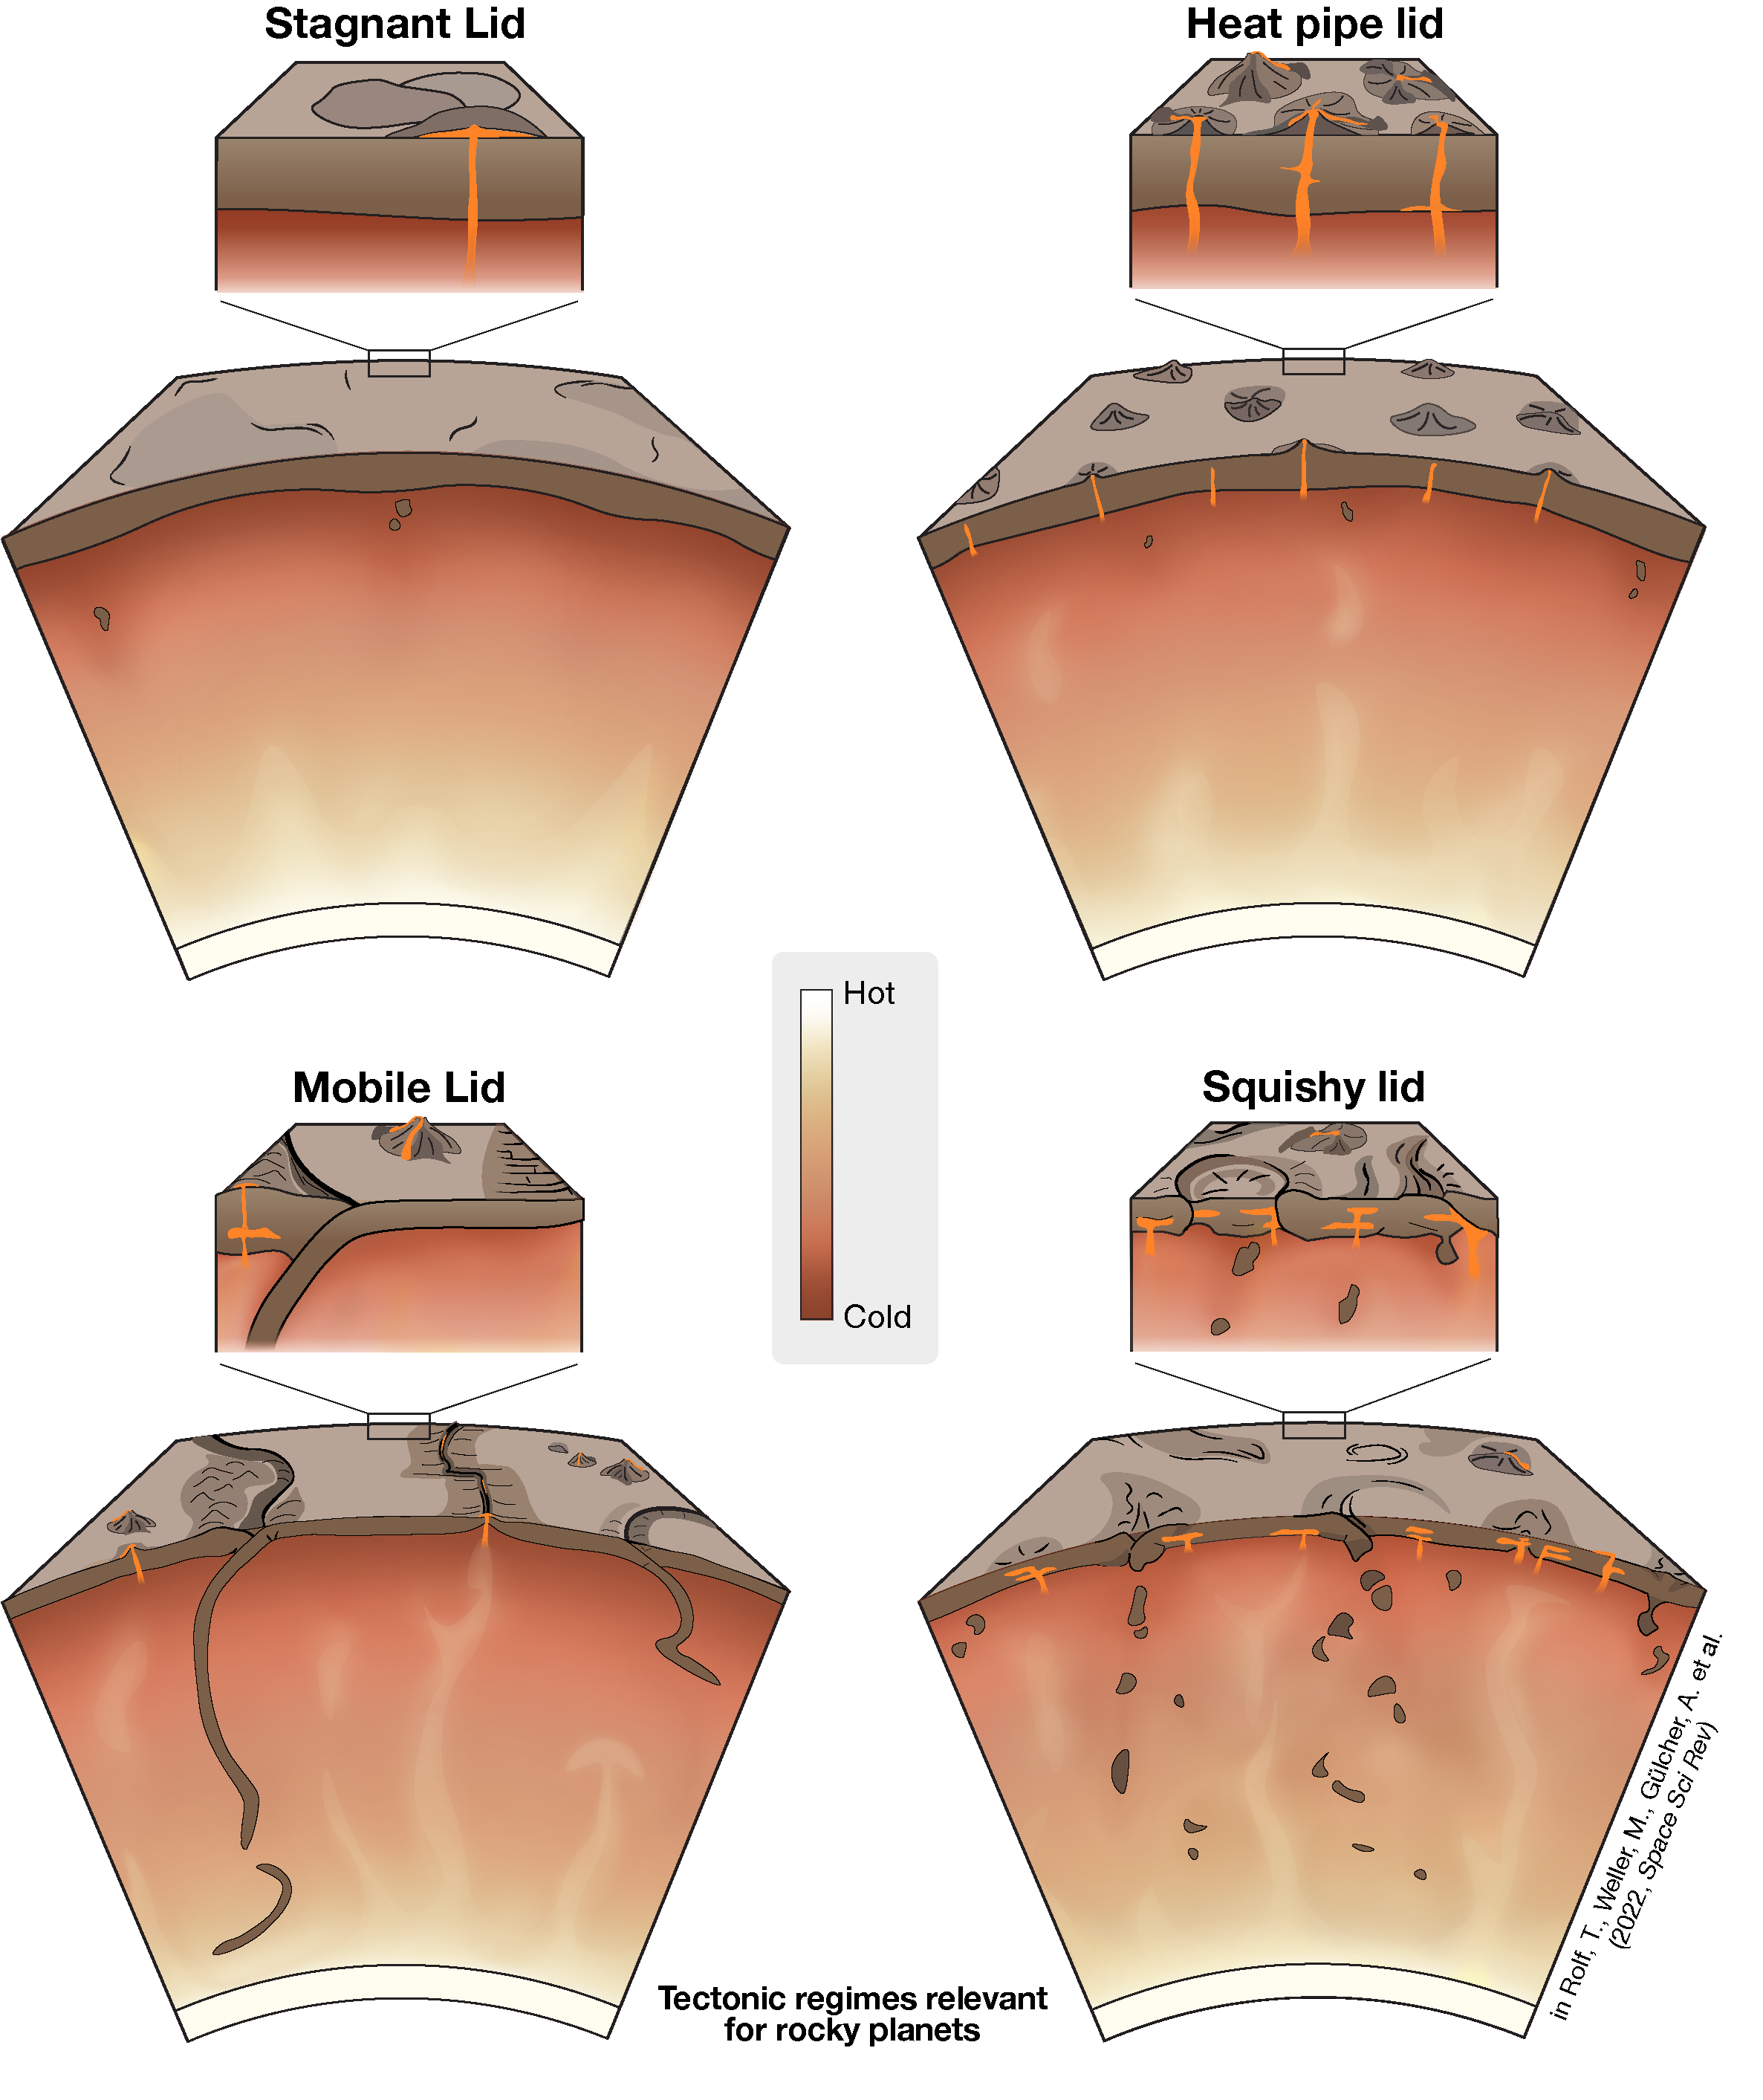
\includegraphics[width=\linewidth]{tectonic_regimes_AG}
\caption[Schematic of the four modalities of planetary tectonic style.]{Schematic of the four modalities of planetary tectonic style. See text for explanation. These graphics by Anna G\"ulcher from \citet{rolf_dynamics_2022} are available via the open-access s-Ink.org repository.}
\label{fig:tectonic_regimes}
\end{figure}



\subsection{Surface heat flow and tectonic mode}
\label{sec:intro-tectonicmode}

Tectonic ``mode'' or ``regime'' refers to the style of mechanical interaction between the outer, rigid layer of a planet and its convecting mantle. Where I have mentioned how the same parameterised model structure cannot arbitrarily be extrapolated to all geodynamic regimes \citep{seales_assessing_2019}, tectonic mode diversity is one of the most tangible reasons why rocky planets would be described by such different regimes. Four distinct tectonic modes are illustrated in Fig. \ref{fig:tectonic_regimes}. Stagnant lids are distinguished from mobile lids\footnote{Plate tectonics are a special case of mobile lids with highly localised deformation.} by how easily the lithosphere yields to plastic deformation---and hence can fail and subduct---whilst extreme cases of intrusive magmatism or extrusive volcanism can also alter  heat fluxes so much as to effect separate tectonic modes:
\begin{enumerate}
\item \textit{The stagnant lid mode} is associated with thick, insulating lithospheres that do not particpate in convection at all (Fig. \ref{fig:tectonic_regimes}, upper left).
\item Surfaces of planets in \textit{the mobile lid mode} move about as quickly as the mantle convects on average. The lithosphere participates in convection and is recycled into the mantle (Fig. \ref{fig:tectonic_regimes}, lower left). 
\item High rates of extrusive volcanism characterise \textit{the heat pipe mode}, with magma thought to pass through the lithosphere in narrow pipes, bringing down mantle temperatures (Fig. \ref{fig:tectonic_regimes}, upper right). This mode is thought to represent the extremely volcanic moon Io, and possibly many terrestrial planets whilst they are young \citep{moore_heatpipe_2013, moore_heatpipe_2017}.
\item \textit{The plutonic squishy-lid mode} also sees high rates of melting, although most of this melt does not extrude at the surface, instead remaining as warm, weak regions in the lithosphere. Denser mineral phases can then drip into the mantle (Fig. \ref{fig:tectonic_regimes}, lower right). This mode has been proposed for modern-day Venus, and could explain some of its observed surface deformation in absence of plate subduction \citep{lourenco_plutonicsquishy_2017, lourenco_efficient_2018, lourenco_plutonicsquishy_2020}.
\end{enumerate} 

A major effect of tectonic mode with regards to (parameterised models of) thermal convection is that it will modify the relationship between convective vigour and surface heat flux (the parameter $\beta$ in \eqref{eq:Ra-Nu}). This has consequences for internal cooling feedbacks, which I discuss in section \ref{sec:background-feedbacks}. Subduction of cold lithosphere is an efficient way to cool the mantle \citep{breuer_dynamics_2015}; so is volcanism, which is expected to be limited on stagnant lid planets with thick lithospheres  \citep{oneill_geological_2007, kite2009geodynamics, noack2014can, noack_volcanism_2017}. Hence stagnant lid planets will trap heat and run hotter, compared to those with mobile lids, for the same $R_p$. A related consequence is that the cores of stagnant lid planets might also cool inefficiently, weakening outer core convection and therefore the possibility of a geodynamo \citep{nimmo_why_2002, driscoll_thermal_2014}. 


Beyond heat transfer explicitly, tectonic mode is also an extremely important control on the chemical cycling between planetary surface and interior. Limited volcanism presents problems for the supply of fresh, weatherable surface rock, or atmospheric gases---a phenomenon explored in Chapter \ref{chapter:outgassing} of this thesis. Plate tectonics on Earth, meanwhile, with its dynamic outgassing of mantle water and subduction of hydrated crust, has helped stabilise the area of exposed continents for about half of Earth history \citep{kasting_what_1992, korenaga_global_2017, honing_longterm_2018}. Whereas subducting plates then carry surface material to the mantle, whether or not other regimes can close the circuit is unclear. We do not know how effectively planets without plate tectonics bury crustal carbonate to help regulate their atmospheric \ce{CO2}, for example \citep[e.g.,][]{elkins-tanton_volcanism_2007, foley_carbon_2018, honing_longterm_2018, honing_carbon_2019, honing_early_2021, rolf_dynamics_2022}. %The surface of stagnant-lid Mars appears to be billions of years old, implying that material has been stuck there for as long \todo{(REF)}. 




I highlight tectonic modes here because they are certainly something we will have to assume, at the moment, whenever we build a thermal evolution model. It is not currently possible to predict what mode a planet is in \textit{a priori} \citep{korenaga_plate_2012, lenardic_notion_2012, lenardic_solar_2016, weller_evolution_2018, ballmer_diversity_2021}; the case of Venus illustrates how this is difficult even having observations of the planetary surface in hand \citep[e.g.,][]{davaille_experimental_2017, rolf_dynamics_2022}. The literature is split between the stagnant lid or plate tectonics mode as the popular choice in model design. One reason to assume Earth-like plate tectonics in our models is that we already know this mode is able to sustain the geochemical cycles thought to stabilise the climate and support life as we know it. Yet because the physics of plate tectonics is also more complicated, the model implementation is less straightforward in practice (for example, one might need to assume the total length of subduction zones). Further, we have not settled on an explanation for why plate tectonics develops on certain planets (including on Earth!), whilst stagnant lids are widely reproduced in analogue laborarory settings and in numerical models, as discussed in the next section. In this thesis, I opt for the stagnant lid regime when I model planetary thermal evolution in Chapters \ref{chapter:topography} and \ref{chapter:outgassing}.


%relevant for thermal history because plate tectonics would somewhat decouple q_sfc from T_m --- because the mantle is ingesting cold lithosphere --- whilst stagnant lid lowers q_sfc for the same T_m - less efficient heat flux - compared to ``classic" Ra-Nu scaling thermal history model 






\subsubsection{The stagnant lid planet as a ``default'' mode}


Stagnant lids (Fig. \ref{fig:tectonic_regimes}, upper left) appear to be a natural consequence of temperature-dependent convection. Laboratory experiments observing scaled-down cells of convecting syrup show that if the viscosity increases sufficiently with decreasing temperature, the cold surface of the convecting cell will be so viscous as to not flow with the convection at all, forming a ``lid'' \citep{davaille_transient_1993, giannandrea_variable_1993}. Numerical experiments have replicated this behaviour at larger scales  \citep{solomatov_scaling_1995, moresi_numerical_1995, solomatov_can_1996}. Heat flows through the lid via conduction, while convection occurs only below the lid, where conditions are hotter and less viscous \citep{morris_boundarylayer_1984, christensen_convection_1984, hansen_high_1993, solomatov_scaling_1995}. Here, the stable stagnant lid is distinct from the upper thermal boundary layer, which is convectively unstable.

Silicate rock has a strongly temperature-dependent rheology \citep{karato_rheology_1993}. %, and indeed the Moon and Mars seem to behave as if they have a stagnant lid \todo{in what sense?}. 
In our own solar system, rocky planets are more frequently found in a non-plate tectonics regime than in a plate tectonic regime \citep{stern_stagnant_2018}. %This fact inspires many questions about whether stagnant lid planets can form ``continents" and other topographic complexities. The character of certain tesserae on Venus imply tectonic origin, questioning whether this world always had a purely stagnant lid \citep{Bindschadler1991, Lenardic1991}. 
The small-number statistics of the solar system bodies do not help much to answer how common plate tectonics is in the universe. Nevertheless, accepting the hypothesis, ``stagnant lids represent the default state of a planet'', might be more justified than applying Earth's plate tectonics to other planets, before we can explain why it began on our world in the first place. %In contrast, our theory of how stagnant lids develop is supported numerically and empirically.
%in justifying that until we know any better we can assume SL is at least plausible, which is perhaps more justifiable than assuming PT because Earth has it, since we can't explain why Earth has it but we can explain why other planets would have SL.}





%Maps of convective regimes in viscosity contrast-Rayleigh number space can be found in \citet{solomatov_can_1996} and more recently in \citet{huttig_regime_2011} and \citet{miyagoshi_thermal_2015}, with stagnant lids favoured by higher Rayleigh numbers \textgreater~$10^{6}$--10$^{7}$ and viscosity contrasts \textgreater~$10^4$ between the interior mantle and the surface.


%For practical reasons, this thesis considers a stagnant lid regime under the premise that it represents a ``default" rocky planet \citep{stern_stagnant_2018}. With the assumption of a stagnant lid we avoid some unknown complexities that mobile plates introduce. %Namely, plate margin-dominated heat loss on Earth works differently \citep[and more efficiently---stagnant lid planets will run hotter for the same rheology and surface heat flow;][]{stevenson_styles_2003} than in a stagnant lid regime, where heat loss is simply determined by boundary layer scaling laws like those we have discussed.


%\begin{figure}
%  \centering
%  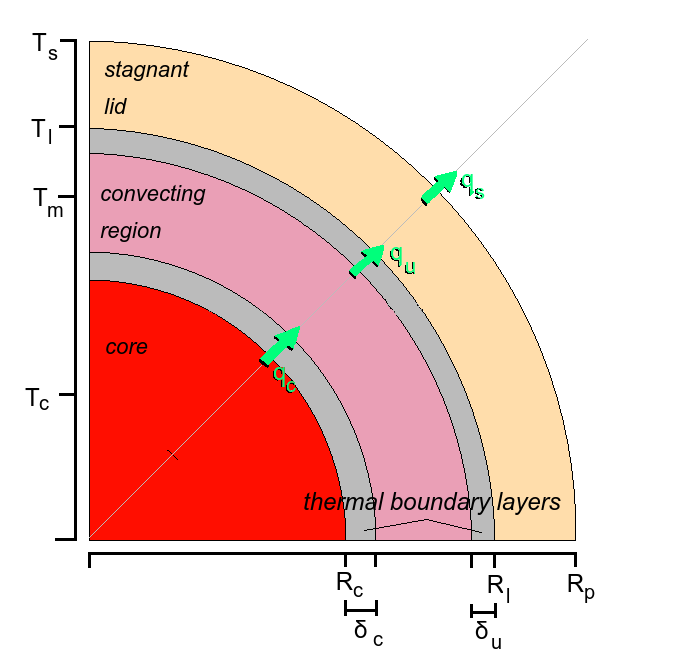
\includegraphics[width=0.5\linewidth]{stagnantlid}
%\caption{Structural model of a stagnant lid planet, not to scale. $R_p$ is the radius of the planet, $R_l$ is the radius at the base of the lid, $R_c$ is the radius of the core, $T_s$ is the surface temperature, $T_l$ is the temperature at $R_l$, $T_m$ is the isothermal convecting cell temperature, $T_c$ is the isothermal core temperature, and $\delta_u$ and $\delta_c$ are the upper and lower thermal boundary layer thicknesses respectively. The boundary layer heat fluxes $q_c$ and $q_u$ and the surface heat flux $q_s$ are defined in equations (\ref{eq:q_Ra}) and (\ref{eq:q_s}), respectively}. 
%\label{fig:stagnant_lid}
%\end{figure}




%
%\subsubsection{The solar system's tectonic garden}
%
%Stagnant lids are differentiated from mobile lids\footnote{Plate tectonics are a special case of mobile lids with highly localised deformation}) by how easily the lithosphere yields to plastic deformation \citep{rolf_dynamics_2022}. I have mentioned that stagnant lid planets cool inefficienlt because
%in the stagnant lid regime, heat conducts ineffiecinetly through the lid because it is so thick. However, planets can also lose heat by magmatism, and even planets with low-velocity lids can have magmatic styles that are different enough to put them into another tectonic regime. The heat pipe regime is characterised by high rates of extrusive volcanism, with magma thought to pass through the lithosphere in narrow pipes.}
%
%
%
%\todo{Other regimes ... heat pipe and squishy lid... newer. kind of cool in between that does involve some chemical interaction via plutonism. believed for venus. they avoid one of the possible issues of true stagnant lids in nature which is that they would be really hot maybe too hot because inefficient heat loss. stuff probably wants to melt!}
%





\subsection{Planetary self-regulation and determinism}
\label{sec:background-feedbacks}
% if this section is here then tie to beta in Ra-Nu relationship. positive beta implies feedback, convective vigour and heat loss are coupled. smaller beta imples more decoupled, negative beta has been suggested for PT..

Inherent to the thermal history of planets, and indeed recognised since the first convection models, are the dynamic feedbacks that regulate mantle temperatures over geologic time. The presence of these feedbacks will be implicit to the results of Chapters \ref{chapter:topography} and \ref{chapter:outgassing}. %\todo{in such a way that makes predicting them a lot more viable.} 
\citet{lenardic_internal_2022} argue that feedback loops in mantle convection deserve just as paradigm-shifting a status as the Daisyworld of climate homeostasis \citep{lovelock_atmospheric_1974, watson_biological_1983}, or of course \citeauthor{walker_negative_1981}'s (\citeyear{walker_negative_1981}) silicate weathering thermostat. That is, in much the same way as feedbacks which stabilise surface temperatures prolong the ``habitable lifetime'' of a planet, feedbacks which stabilise mantle temperatures will also prolong the geodynamic lifetime of a planet. The possibility of mantle self-regulation should also be of strong practical interest to exoplanet researchers because it entails that mantles will lose the memory of their initial state, such that---from a modelling standpoint---much of the stochasticity inherent in forming planets can be removed. Understanding these feedbacks might help us judge whether certain phenomena of Earth are likely a fluke of thermal history \citep[e.g., the fact that the temperature near the top of the mantle is very close to the melting temperature of peridotite;][]{seales_buffering_2022}, or if these phenomena are also representative of other planets. At the same time, feedback loops can be a double-edged sword if they lead to multiple stable solutions for a planet's evolution---perhaps Earth and Venus followed diverging paths from simiar initial conditions \citep{lenardic_solar_2016}.

The most fundamental feedback regulating thermal evolution follows from the temperature-dependence of mantle viscosity \citep{tozer_present_1972}. Decreasing temperature raises viscosity, which leads to less vigorous convection, and less heat flow out of the mantle, which in turn heats the mantle and lowers its viscosity. This feedback would buffer the interior at a near-constant viscosity, even as its internal heating rate decreases with exponential radionuclide decay, a corollary of which is a narrow range of mantle viscosities for rocky exoplanets. This \citeauthor{tozer_present_1972} feedback has not been proven to occur on Earth, hence it is not guaranteed to occur on other planets either \citep{korenaga_can_2016}; its efficiency depends on whether the heat flux out of the mantle can adjust quickly enough to a change in temperature. Parameterised models capture response time via the $\beta$ parameter in \eqref{eq:Ra-Nu}, for which the classic value of 1/3 corresponds to quick response time and self-regulation \citep{seales_assessing_2019}.

Theory suggests that stagnant lid convection ($\beta \approx 1/3$) should always meet this short thermal response requirement, at least on an Earth-mass planet \citep{korenaga_can_2016}. Less is understood about the rheological behaviour of rock at the several-hundred-GPa pressures found in planets more massive than Earth, but we would at least expect viscosity to increase with pressure \citep{christensen_convection_1984}---the strength of the pressure-dependence may preclude viscosity self-reguation \citep{stamenkovic_influence_2012}, or may not \citep{tackley_mantle_2013}. As for planets with plate tectonics, $\beta$ depends on the extent to which plate motions are governed by mantle convection \citep[as opposed to, e.g., the plates' own strength;][]{conrad_effects_1999, crowley_analytic_2012}; $\beta$ here could be 0 or even negative \citep{korenaga_energetics_2003}. The parameterised convection model I use in Chapter \ref{chapter:topography} considers stagnant lid convection heated from below with $\beta \approx 1/3$.
%other feedbacks exist and are reviewed in lenardic & seales. 



%\todo{In any case the Earth controversies are useful to us now because they emphasise how low Ur (non thermally self-regulated ) systems can't exist  with  classical or stagnant lid style heat loss}

%\todo{The above argument also points out that classical models which are tuned to earth are actually wrong in that they don't even meet earth's constraints. so would be careful to do this. is there an example? like turcotte 2002 etc. better to use stagnant lid model with semi-empirical scalings?}


In any case, the generally-high thermal inertias of mantles means that with the natural decay of an internal heat source, they never do reach true thermal steady state \citep[cf.][]{tozer_present_1972}. Rather, planets cool down, perhaps in a series of quasi-steady states, until geodynamic death (no energy for mantle convection)---if they are not first swallowed in their star's asymptotic giant branch stage, that is. All planets therefore have a natural end to their convective, tectonic, and volcanic activity, possibly foretold by the size and heat-producing element budget with which they are born \citep{stevenson_styles_2003, frank_radiogenic_2014, unterborn_mantle_2022}. Luckily, these two parameters could be amenable to observation \citep{nimmo_radiogenic_2020, wang_europium_2020}. In this way it should be sensible to estimate the thermal histories of generic stagnant-lid planets.


























%
%\subsection{Two consequences of heat transport}
%
%\todo{In this thesis are two direct explorations of mantle thermal convection controlling surface properties}
%
%\subsubsection{The shapes of planets}
%
%\subsubsection{Volcanism and volcanic outgassing}












\section{Geology in the cosmos}
\label{sec:background-composition}
Section \ref{sec:background-thermalhistory} has presented the tools used to assess how planets evolve thermally over billions of years. Here I discuss what sets planets' material properties---properties which, in a pragmatic sense, will go into these thermal history models, but should also, in a broader ontological sense, influence the \textit{geologic} evolution of planets in complex ways we are just beginning to formalise. Namely, planets' interior compositions add another axis to their potential diversity. By ``composition'', exoplanet researchers can be referring to the first-order concentric structure of a planetary interior---the relative sizes of metallic, silicate, and volatile layers---as well as to higher-order concerns, such as abundances of specific elements or minerals in the mantle. The bulk element composition a planet inherits from its formation, in terms of the major rock-forming refractories but also volatiles like H and C, sets up its subsequent thermal evoluton via composition-dependent properties (e.g., viscosity parameters, solidus temperatures, oxidation state) and boundary conditions. Planetary differentiation---the segregation of iron and siderophile elements as a metal core to a planet, and the partial melting of a mantle forming a crust enriched in incompatible elements---means that these inherited elements become heterogeneously distributed within a single planet. Nevertheless, as I introduce throughout this section, inter-planet compositional diversity need not be infinite in every way despite the high entropy of the universe.

To the first order, the interior composition of a planet is linked to its bulk density: metal is denser than silicate, which is denser than ice or gas. When observers try to piece out the interior structure of a given exoplanet, however, they are blocked by a certain degeneracy: density provides two data in the planet mass and radius, but there are at least three possible compositional layers in a metal core, silicate mantle, and volatile envelope. A larger core, thinner mantle, and thicker volatile envelope would produce the same density as a smaller core, thicker mantle, and thinner volatile envelope. There is additional degeneracy from the possibility of a planet's silicate portion to be molten, if hot enough \citep[inducing $\sim$10\% density variations;][]{bower_linking_2019}, and less so, from the fact that the iron core could contain an unknown proportion of light elements such as Si and O \citep{unterborn_scaling_2016}. This degeneracy is the famous major problem of exoplanet interiors in the observational community. Such degeneracies prohibit a clean identification of water-poor, rocky planets (note Earth is water-poor, with its surface oceans contributing just $\sim$200~ppm of its mass). For example, four of the roughly Earth-mass planets orbiting the TRAPPIST-1 star, which appear to be $\sim$10\% less dense than Earth, could consequently have water mass fractions between $\sim$0--10\% depending on their unknown core sizes \citep{unterborn_inward_2018, agol_refining_2021}---enough water to preclude any dry land, as I show in Chapter \ref{chapter:topography}. 

I am mentioning this astrophysical barrier first because \textit{(i)} it is a good example of the limits to current knowledge from specific exoplanet observations alone, and \textit{(ii)} the reader should understand what this thesis is not aiming to resolve. Precise predictions for individual planets need not be our focus---although contributions from Earth science will certainly be needed to gather other constraints on planets' metal core sizes (section \ref{sec:background-redox}). For example, I am not interested in exoplanet chemical compositions for the sake of \textit{identifying} known planets as ``Earth-like'' or not, since I believe that such categories, which necessarily rely on a few state variables, are only ever going to mislead. To that end, higher-order mantle mineralogy, which in general does not lead to serious bulk density differences \citep{dorn_can_2015, unterborn_scaling_2016}, would not seem as important for interpreting the astrophysical mass-radius observations;\footnote{\citet{dorn_new_2019} present an exception: planets that are hypothetically rich in high-temperature condensates Ca and Al, for example because they form \textit{in situ} very close to their star, would be noticeably (10--20\%) less dense than Earth or Venus.} many astronomers are happy to consider mantles as pure \ce{MgSiO3} as such. The converse is that because mineralogical diversity is largely unrelated to bulk densities---and indeed, this diversity is best inferred by other observational means (the next section)---studies of exoplanet mineralogy are freed from the above degeneracy.


The fairly recent illumination of the rocky exoplanet composition axis is unforaged ground for researchers. That is, it opens new ways to approach the Big Question,\footnote{Are we alone?} and new needs for experimental work. Mantle mineralogy must surely be a consequential %\textit{and constrainable} 
state variable in the comparative thermochemical evolution of planets. The minerals stable through a mantle will affect, for example, its rheology \citep[e.g.,][]{spaargaren_influence_2020}---but in contentious directions \citep[ferropericlase may be stronger or weaker than bridgmanite; cf.][]{yamazaki_mineral_2001, cordier_periclase_2023}---its melting temperatures \citep[alkalis, Fe, and higher Ca/Al ratios depress the solidus;][]{hirschmann_mantle_2000, kiefer_effects_2015, brugman_experimental_2021}, and its volatile budget (Chapter \ref{chapter:rockywater}, this thesis). For a given geotherm, they will determine crust compositions \citep[e.g.,][]{fortin_volcanic_2022}: pyroxenes and quartz melt at lower temperatures, suggesting thicker crusts \citep{lambart_role_2016}, as do FeO-rich compositions in general \citep{dyck_effect_2021, wade_divergent_2017}. Crusts, being the result of extra processing, have much more geochemical complexity (i.e., less modelling tractability) than mantles, but are worth some more elaboration here. Their variable thickness brings still more complexity to the previous section's thermal history concepts: \textit{(i)} U, Th, and K are incompatible such that thicker crusts remove more heat-producing elements from the mantle; and \textit{(ii)} crusts can reduce conductive heat loss \citep{lenardic_continental_2005, lenardic_note_2011}. Less understood but very important is how crust composition could affect the tectonic regime, given that some lithologies will be more deformable \citep[lower yield stress to plate formation; e.g.,][]{karato_remarks_2014, weller_evolution_2018, ballmer_diversity_2021}. %, whilst thick basaltic crusts could also self-destabilise if they reach eclogite transition pressures \citep{orourke_terrestrial_2012}---there is a complex relationship between mantle mineralogy, crust composition and thickness, and lithosphere strength. 
Dimensions like these are worth pursuing not only for curiosity reasons  \textit{(what kinds of planets could be out there?)}, but also because understanding what planets are capable of without life is necessary for attributing biologic origin to any signal \citep{wordsworth_redox_2018, lisse_geologically_2020, krissansen-totton_oxygen_2021, krissansen-totton_understanding_2022, butkus_note_2023}.



One community which has shown itself as incredibly well-poised to help understand exoplanet geology is that of the theoretical mineral physicists. The existence of a large population of massive rocky planets implies the existence of mantle rocks at extremely high-pressures: up to $\sim$630~GPa at the core-mantle boundary, versus 136~GPa on Earth \citep{unterborn_pressure_2019}. As such, research into Earth's deep mantle naturally extends to exoplanets. Density functional theory, \textit{ab initio} molecular dynamics, and machine learning have been vital in predicting the high-pressure material propreties---particularly, rheological and melting properties---of known lower mantle phases like postperovskite and ferropericlase \citep[e.g.,][]{tackley_mantle_2013, stixrude_melting_2014, millot_shock_2015, sakai_experimental_2016, ritterbex_vacancies_2018}, but also the alien mineral phase transitions that occur beyond postperovskite \citep[e.g.,][]{umemoto_twostage_2011, umemoto_phase_2017, coppari_implications_2021}. Theoretical equations of state of postperovskite agree very well with experimental data up to $\sim$300~GPa, for example \citep{sakai_experimental_2016}. These high-pressure mineral properties and phase diagrams are currently a source of uncertainty in comparative planetary evolution research---but with this discipline's enthusiastic pace, we might soon approach the limit of what is technologically possible to constrain.




\subsection{The chemical diversity of stars (and their planets)}
\label{sec:background-starchem}
% in this section should actually say what some of these are... maybe with ternary diagram?

The crux of rocky planet composition insight is that planets are chemically linked to their host stars. A star and its planets grow from the same nebular cloud; stars contain \textgreater 99\% of the mass, so their elemental compositions---which are spectroscopically observable---are a good proxy for those of the nebula. Most atoms in stars may be hydrogen or helium, but if we remove these and consider only the major rock-forming, refractory elements (Mg, Si, Fe, Ca, and Al), then is it not likely the condensing building blocks of planets inherit the same relative inventory of these elements? This behaviour exactly has been replicated in planet formation simulations \citep{bond_compositional_2010, thiabaud_elemental_2015} and is consistent with an observational pilot study \citep[discussed below;][]{bonsor_hoststar_2021}. If true, then the measureable compositional diversity of stars---the variability in their refractory element ratios---may therefore inform the compositional diversity of planets. 

Namely, main sequence stars have different element abundances because they form in different parts of the galaxy with their own local chemical evolution \citep{hinkel_stellar_2014}, but not \textit{too} different because they still obey the same rules of nucleosynthesis \citep{burbidge_synthesis_1957}: they will always contain greater abundances of Si, Mg, and Fe, for example, than Ti and Cr (being other, minor rock-forming elements). The releative proportions of refractory elements determine which mineral phases are stable as a function of temperature and pressure in the mantle. Simple stoichiometry tells us that increasing Mg with respect to Si favours forsterite (the olivine endmember \ce{Mg2SiO4}) over enstatite (the orthopyroxene endmember \ce{MgSiO3}) because the former takes two Mg atoms per Si atom. I use this example because Mg/Si has the largest effect on modal mantle mineralogy---and hence is quoted sometimes as a proxy---because Mg and Si are the most common elements is silicate rocks apart from oxygen. In the Hypatia Catalog of nearby FGKM stars, 68\% of measurements show Mg/Si between 0.91 and 1.35 \citep{hinkel_stellar_2014}; i.e., most rocky planets are pyrolitic. That planet-hosting stars have minor variations in their element abundances is a major premise of the second half of this thesis. 



When stellar element abundances are used to estimate exoplanet mantle mineralogies, wholly foreign compositions (with respect to the solar system) do not appear \citep{hinkel_star_2018, putirka_composition_2019, wang_enhanced_2019, wang_detailed_2022, spaargaren_plausible_2022}. Given the broad consistency between stellar abundance patterns, phase equilibria modelling produces only a handful of mineral phases stable at mantle conditions: olivine polymorphs, pyroxenes, spinel, and garnet in the upper mantle, and (post)perovskites and ferropericlase (also known as magnesiow\"ustite) in the lower mantle, with possible silica phases (quartz, coesite, stishovite) stable in the most Si-rich cases. The exception is in the deep lower mantles of $\sim$4-Earth-mass planets and up, where \ce{MgSiO3} postperovskite has been predicted to recombine into new phases above $\sim$0.5 TPa \citep{umemoto_phase_2017}. Robust predictions of these high-pressure mineral phase equilibria are only as good as the thermodynamic (theoretical and experimental) data. Yet our datasets are always expanding, such as the thorough, probably painstaking compilation of \citet{stixrude_thermal_2022}, which accounts even further for the realistic thermodynamics of solid solutions.\footnote{For example, in the \citet{stixrude_thermal_2022} dataset, the ``perovskite'' phase is a solid solution of \ce{Al2O3}, \ce{FeSiO3}, and \ce{MgSiO3}.} Chapter \ref{chapter:rockywater} demonstrates how to predict self-consistent phase proportions, adiabatic profiles, and mass-radius relationships for arbitrary (but plausible) refractory compositions of planets up to about 4 Earth masses, before the phase equilibria uncertainties might start to challenge our trust.
%In absense of very extreme partitioning scenarios, these nucleosynthesis patterns mean that we do not expect graphite/diamond planets, aluminium planets, \textit{etc.} to exist \todo{(REF?)}.
% cf. madhu 2012 ApJL, born
% can't find formation model precluding carbon planets... wilson+ 2016 find no evidence  for C-rich planetary material from PWD C/O measurements, also jura & young review says this, but haven't introduced WDs yet at this point


%Out of the various element ratios, Mg/Si has the biggest effect on modal mineralogy---hence it is quoted sometimes as a proxy---because Mg and Si are the most common elements is silicate rocks apart from oxygen. Simple stoichiometry tells us that increasing Mg/Si favours forsterite (the olivine endmember \ce{Mg2SiO4}) over enstatite (the orthopyroxene endmember \ce{MgSiO3}) because the former takes two Mg atoms per Si atom. %If Mg/Si $\gtrsim$ 1.5 then no orthopyroxene stabilises; whilst if Mg/Si $\lesssim$ 0.7, there is no stable olivine, and the excess Si will form silica phases. Compositions richer in Al will stabilise more spinel and garnet, although aluminous phases are not expected to make up more than half the mass in the olivine stability field. 


% [What stoichiometry is Si-limited to make olivine and where does that Mg go?],

% therefore broadly get the same minerals as in earth, which thermodynamic phase diagrams (plus simple stoichiometry) show us are the stable phases:  




% Mars Mg/Si=0.88 (Yoshizaki & McDonough 2020)
As I write this, the preservation of refractory ratios between planet and star remains a \textit{fundamental assumption} and a \textit{working hypothesis}. The solar photosphere's measured Mg/Si ratio (1.05), whilst virtually exactly the same as CI chondrites within error, notably underestimates the value of 1.27 canonical for Earth's upper mantle \citep{ringwood_significance_1989, palme_solar_2014}. A robust explanation of this misfit would close a conspicuous knowledge gap in exoplanet research. It is conceivable that our models of the Bulk Silicate Earth composition are simply not sampling the entire mantle, insofar as they are based on upper mantle xenoliths \citep{matas_bulk_2007, javoy_chemical_2010}, though some analyses have argued against this \citep{lyubetskaya_chemical_2007a}. However, Mg and Si also could have relatively fractionated through a dynamic process as the Earth and other planets accreted, despite the 30-K difference in their 50\% condensation temperatures \citep{ringwood_significance_1989, miyazaki_dynamic_2020}. Even more likely is that some Si enters the metal core and is trapped there \citep{ringwood_chemical_1959, javoy_integral_1995, Wood2006, schaefer_metalsilicate_2017}; some estimates of Earth's core Si content are up to $\lesssim$10 wt.\% \citep{wade_core_2005, ricolleau_oxygen_2011, fischer_high_2015}.  

%how Si partitions into cores and if we can estimate this, which not only affects core densitt as above but also mantle composition, and other processes that partition si with respect to major refractory elements like Mg in the protoplanetary disc (e.g. miyazaki), and how volatiles are delivered to planets?.


As to be expected, the volatile element abundances of planets are much more removed from those of their host stars. Rather than condensing at high temperatures near the centre of the protoplanetary disc, these elements will be transported to the disc's outer regions \citep{ringwood_significance_1989, cassen_models_1996, ciesla_radial_2008}. However, volatiles can then be scattered inwards from gravitational perturbations, and whole planets can also migrate \citep[e.g.,][]{unterborn_inward_2018, raymond_migrationdriven_2018}. Oxygen is a particular nuisance because it can be dually refractory (bound up as oxide components of rocky material; e.g., as \ce{SiO2}) or volatile (e.g., as \ce{H2O}), and Earth's total oxygen budget has not yet been explained unamimously in terms of its stochastic accretion \citep[e.g.,][]{raymond_making_2004, morbidelli_building_2012, rubie_accretion_2015, obrien_delivery_2018, sossi_stochastic_2022}. Further, moderately-volatile alkalis such as Na and K, whilst relatively unimportant for a mantle's mineral proportions, can be quite consequential for its melting behaviour \citep{hirschmann_mantle_2000}. \citet{wang_detailed_2022} make a good start using empirical star-planet depletion trends, based on our solar system, to estimate rocky exoplanet mantle compositions; in Chapter \ref{chapter:fo2} I will take a similar approach when estimating planets' Na compositions. Nevertheless, we do not have the data to evaluate whether this solar system trend is the best model for planetary systems in general. Major theoretical questions linger over the degree to which the ingredients of extrasolar rocky material deviate from stars; an answer begs a good understanding of high-pressure metal-silicate partitioning behaviour and the dynamic chemical evolution of protoplanetary discs.

% Hinkel & Unterborn 2018:
% In general, the error reported for stellar abundances of [Mg/H], [Al/H], [Si/H], and [Ca/H] are 0.07 dex, 0.06 dex, 0.05 dex, and 0.06 dex, respectively (Hinkel et al. 2014). 
%Nissen (2015) reported errors of 0.009 dex, 0.005 dex, 0.005 dex, and 0.006 dex, while Spina et al. (2016) had errors of 0.014 dex, 0.012 dex, 0.007 dex, and 0.013 dex. 

Errors in both planet bulk densities and host star abundances limit predictions about the interior composition of a given planet. In particular, the typical measurement error on individual host star abundances \citet{hinkel_star_2018} propagates to an error on Mg/Si of $\sim$0.2: nearly consuming the Sun-Earth Mg/Si discrepancy. The more problematic type of uncertainty, however, is the spread in reported values between the various techniques used to retrieve abundances from the raw stellar spectra \citep{hinkel_comparison_2016}. A thorough discussion of error propagation from stellar abundances to exoplanet mineralogy can be found in \citet{hinkel_star_2018}. As per the theme of this chapter, what remains tractable is the \textit{range} of stellar refractory ratios, which should inform the minimum \textit{range} of planet refractory ratios, so long as their fractionation processes are minor and roughly universal across protoplanetary discs \citep{bond_compositional_2010, thiabaud_elemental_2015}. (It is already interesting to note that the Sun is very close to the median in terms of Mg/Si/Fe.) From here, the field looks wide open for us to explore and eventually formalise the many ways mineralogy, inherited at birth, determines planet evolution. % very new. lots of experimental petrology work to be done such as the solubility of volatiles (water and carbon) in different mantle rock types (e.g. sossi). 
\citet{spaargaren_influence_2020} have bravely started incorporating mantle mineralogy into thermal evolution models; we are no longer confined to canonical Bulk Silicate Earth as representative of all exoplanet mantle compositions. To model these evolutions most effectively, however, we need more experimental and \textit{ab initio} data on rock viscosities and melting temperatures across the diversity of mantle mineralogies we now expect.  




\subsubsection{More clues from stellar remnants}
\label{sec:background-pwd}



\begin{figure}
  \centering
  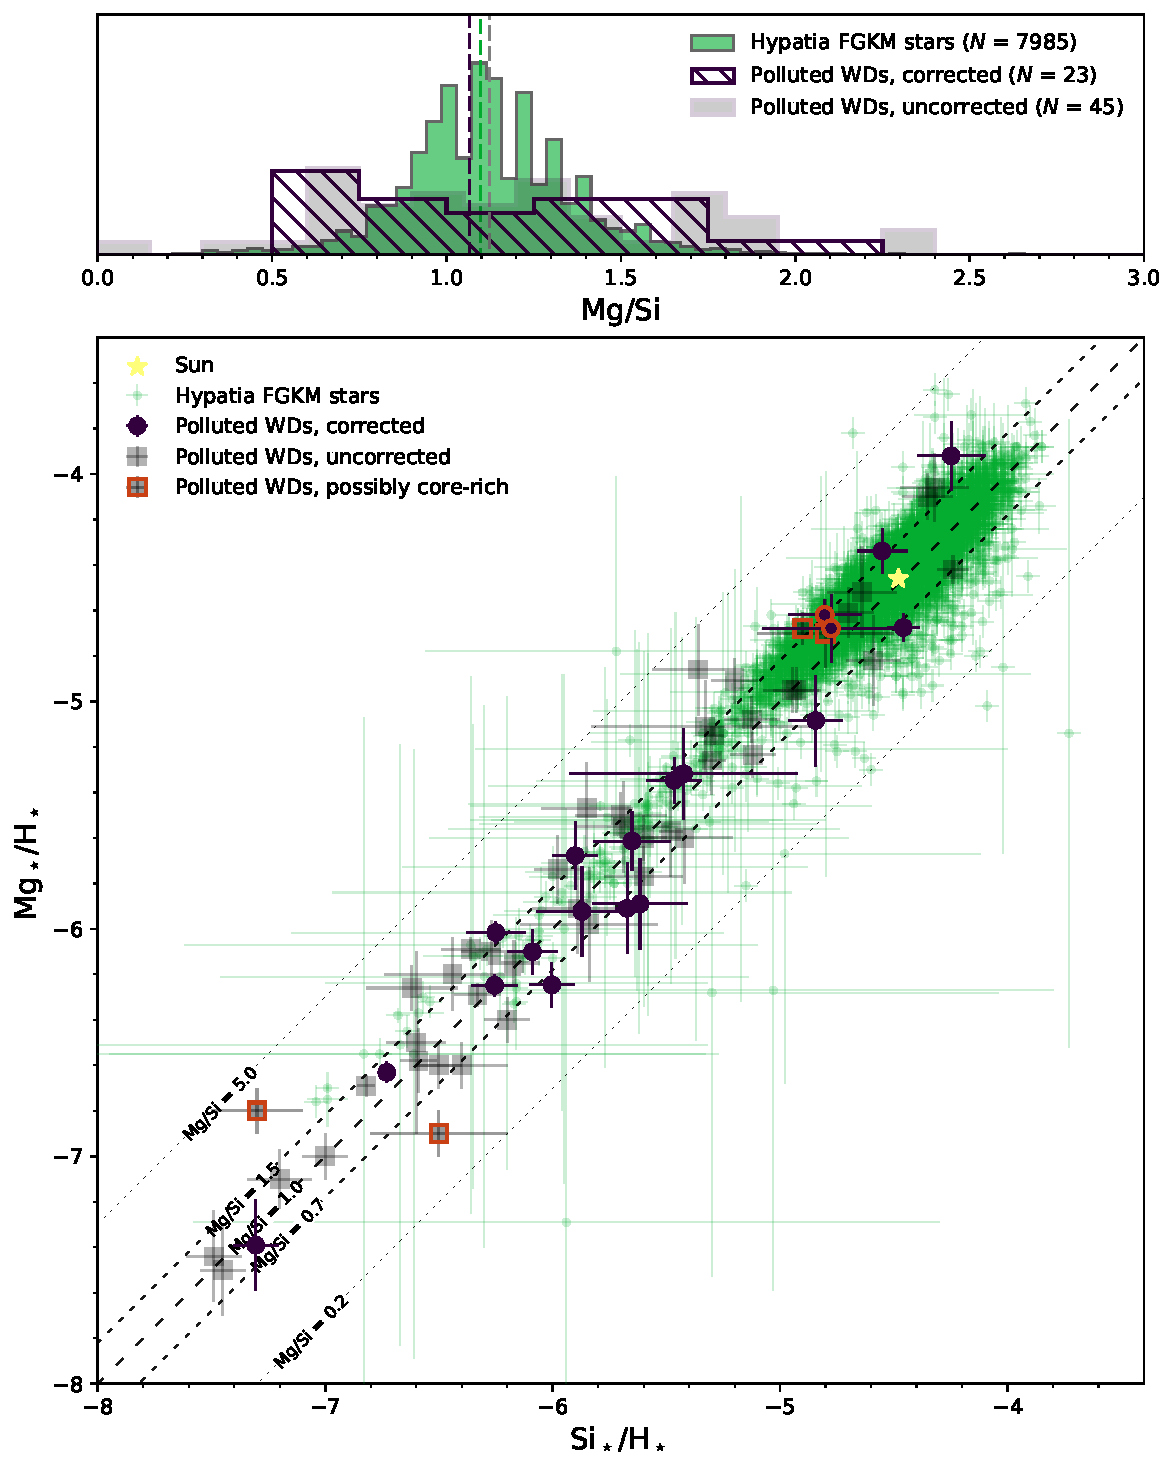
\includegraphics[width=0.95\linewidth]{wd_hypatia_mgsi.pdf}
\caption[Comparing Mg/Si ratios between FGKM stars and polluted white dwarfs, which provide independent constraints on rocky exoplanet bulk compositions.]{Comparing Mg/Si abundances between FGKM stars and polluted white dwarfs (WDs), which provide independent constraints on rocky exoplanet bulk compositions. \textit{(Bottom:)} Observed stellar abundances with respect to H, where the number ratio ${\rm X}_\star/{\rm H}_\star = \log_{10}(n_X/n_H)$ in astronomical notation (note abundances are not solar-normalised). The green dots show all FGKM stars in the Hypatia Catalog$^a$ with measured Mg and Si at time of writing. WD data are from a compilation provided by Andrew Buchan (including unpublished data from Laura Rogers), where the purple circles have been corrected to steady-state accretion by accounting for differential sinking; grey squares are uncorrected; and the points highlighted orange are likely to be core-rich fragments (estimated core mass fraction $> 0.4$). The errors on both data sets are different: the Hypatia Catalog reports errors as the spread between different sets of measurements---which can be quite high---whilst the WD errors are the measurement uncertainties as reported in the original publications. The typical measurement uncertainties of the Hypatia abundances are 0.07 dex for ${\rm Mg}_\star/{\rm H}_\star$ and 0.05 dex for ${\rm Si}_\star/{\rm H}_\star$ \citep{hinkel_stellar_2014}. Diagonal lines denote reference molar ratios: above ${\rm Mg/Si} \approx 1.5$, orthopyroxene disappears from the upper mantle, and below ${\rm Mg/Si} \approx 0.7$, pure-\ce{SiO2} polymorphs become stable throughout. \textit{(Top:)} Histograms of the same data, The vertical dashed lines show the medians.\\ 
\vspace*{10.5em} \footnotesize{$^a$\citet{hinkel_stellar_2014, hinkel_comparison_2016}, https://www.hypatiacatalog.com/}
}
\label{fig:hypatia_vs_pwd}
\end{figure}
%\todo{[todo: find out from Andy which are optical vs UV!]}

There is an independent way to probe (disintegrated) planet compositions through (the afterlives of) stars. Well-established stellar evolution concludes in white dwarfs, stars' collapsed, electron-degenerate remains. White dwarfs are so dense that their photospheres should only contain H or He---the temporary presence of any heavier element would seem to have exogenous origins. We now believe that the exogenous material represents planet(esimals), asteroids, or exomoons from the outer regions of an ancient planetary system,\footnote{i.e., because the star would have engulfed anything within an AU or so during its asymptotic giant phase \citep{veras_postmainsequence_2016}.} ripped apart by tidal forces, and eventually accreted onto the white dwarf \citep{jura_extrasolar_2014}. At least a third of observed white dwarfs are ``polluted" as such \citep{koester_frequency_2014}. Because heavy elements sink through white dwarf photospheres in less than 0.1 Gyr \citep{koester_accretion_2009}, the pollution must have been recent, in astronomical terms---the accretion event itself could be as short as years \citep{rogers_nearinfrared_2020}---and it is commonly assumed that each observed assemblage of pollutants represents a single body: a complete parent body, or post-collisional fragment of \citep{jura_extrasolar_2014}. Observations of heavy element abundances in polluted white dwarfs therefore provide a direct probe into exoplanetary system compositions.


Compared to main sequence star abundances, the measurement uncertainty here is typically higher because the spectral lines of white dwarfs will necessarily have higher gravitational broadening \citep[e.g.,][]{bonsor_hoststar_2021}. Further, a fair amount of modelling is needed if we are to infer parent body and particularly exoplanet compositions from white dwarf photosphere abundances \citep[e.g.,][]{harrison_polluted_2018, harrison_bayesian_2021, buchan_planets_2022}. Any estimation of exoplanet compositions from polluted white dwarfs would want to consider two complications:
\begin{enumerate}[label=(\roman*),font=\itshape]

\item Not much is known \textit{a priori} about the nature of the individual accreted bodies that our measurements are sampling: their mass, degree of metal-silicate differentiation, and---if collisional fragments---the degree to which they contain the parent body's core or silicate mantle, analogous to iron meteorites, stony achondrites, and pallasites from our solar system \citep{bonsor_are_2020, buchan_planets_2022}. However, geochemical constraints such as pressure- (size-) dependent element partitioning may be leveraged to this end \citep{buchan_planets_2022}.

\item Different elements sink at different rates through white dwarf photospheres. These rates depend on the white dwarf's effective temperature, surface gravity, and whether it is H- or He-dominanted; interpreting the observed abundances hinges on whether the accretion is in an ongoing, declining, or steady-state phase \citep{jura_extrasolar_2014}. \citet{brouwers_asynchronous_2023} showed that accretion-timeline uncertainties create artificial variation in inferred parent body oxygen contents. Oxygen sinks relatively slowly, so observing it in excess could actually mean that the accretion event happened a long time ago, rather than that the parent body was O-rich. 

\end{enumerate}
Neglecting these complications may lead to less-significant or possibly misleading results. Accounting for effects \textit{(i)} and \textit{(ii)} may question the number of O-rich white dwarfs reported in \citet{doyle_new_2023}, for example. %Chapters \ref{chapter:rockywater} and \ref{chapter:fo2} sidestep these complications by focusing on the main sequence stars' indirect constraints on exoplanet compositions (opting instead to be hindered by the other complications from section \ref{sec:background-starchem} therein). 

With uncertainties accounted for, observations of polluted white dwarfs can not only clue us to exocosmochemical variability, they can also help corroborate our earlier presupposition that planet refractory ratios equal star refractory ratios. This is possible because white dwarfs provide an independent constraint. \citet{bonsor_hoststar_2021} compared the refractory element composition of the polluted white dwarf WD 1425+540 with its K-dwarf binary pair G200-40 (expected to be chemical twins), showing that the pollutant and G200-40 compositions were alike within error, whilst they differed from a random K-dwarf. Increasingly precise observations of polluted white dwarfs, combined with theoretical developments in how they accrete rocky material, will likely prove invaluable if we want believable constraints on the mineralogy of specific nearby exoplanets.

We can start to make preliminary comparisons between the refractory variability of polluted white dwarfs versus FGKM stars. Figure \ref{fig:hypatia_vs_pwd} shows this comparison for Mg and Si. Polluted white dwarfs appear to show greater dispersion in Mg/Si than the FGKM stars, reflecting the fact that the former measurements sample a range of planetary material which has variously differentiated, fragmented, and otherwise been processed. However, the distribution medians seem very similar (1.10 vs. 1.09 or 1.12 depending on correction). Similar medians would suggest that, on average, the formation and evolution of planets is not systematically fractionating Mg/Si---and hence the proportions of major mantle elements---in a particular direction.




% figure comparing mg/si and mg/fe in WD vs hypatia planet-hosting?

%I think there's an even more fundamental issue which is that (as far as I can tell) they don't consider the possibility of accretion being in declining phase, which is huge. Oxygen generally sinks slowly, so an apparent excess of oxygen could also just be explained by the accretion having already ended a while ago, and everything else has just sunk faster through the white dwarf atmosphere, so you really need to take this into account. (This is one of the key points from this paper https://arxiv.org/abs/2211.05113 ). (They also don't seem to consider the possibility of differentiation + fragmentation, although that's less fundamental). I reran this systems with my model - according to my model only one of these systems (0218) is actually likely to have an oxygen excess. - Andy


\subsection{The importance of core size, and attempts to constrain it}
\label{sec:background-redox}
% keep this section very short because it could be a rabbit hole lol

To complete the circle, there is a useful future role for Earth science in interpreting planet composition constraints, for the purpose of ameliorating the ruesome bulk density-interior structure degeneracy (section \ref{sec:background-starchem}). Because this degeneracy exists due to unconstrained metal core sizes, geochemical limits to core formation may therefore offer some insight into exoplanets' interior structures. Metal cores form according to the equilibrium:
\begin{equation}
\label{eq:background-iw}
\ce{Fe^{\rm metal} + \frac{1}{2} O2 <=> FeO^{\rm silicate}}.
\end{equation}
Here, iron is undergoing redox reactions within young planets' magma oceans---the stage during which planets are so hot from accretion energy and short-lived radionuclides to be largely molten \citep{elkins-tanton_magma_2012}---where the dense metallic iron eventually sinks to the planet centre \citep{kleine_rapid_2002, yin_short_2002, wade_core_2005, Wood2006}. Importantly, equilibrium \eqref{eq:background-iw} need not go to completion. Some FeO could remain in the mantle such that the final core mass fraction will be related to the molar ratio of Fe-metal to FeO, $X_{\ce{Fe}}^{\rm metal}/X_{\ce{FeO}}^{\rm silicate}$. Indeed, Earth's mantle contains $\sim$8~wt.\% FeO \citep{mcdonough_composition_1995}. At this stage, lighter elements such as Si may also become involved in iron redox equilibria, subtly co-modulating the final core and mantle compositions \citep{wade_core_2005}.

%Core light element compositions are also co-modulated with the magma ocean oxidation state by equilibria such as \ce{SiO2^{\rm silicate} + 2Fe^{\rm metal} <=> 2FeO^{\rm silicate} + Si^{\rm metal}}.% Hence, principally, core size and density reflect how oxidising the magma ocean is, which is gauged by the oxygen fugacity (a concept that Chapter \ref{chapter:fo2} will explain in detail). 

Although we do not have a way to predict how oxidising a magma ocean should be \textit{a priori}, there are two hard, natural limits to the iron core mass of a planet. If all the iron in the magma ocean is oxidised (equilibrium \eqref{eq:background-iw} is all the way to the right), then the minimum core mass is zero---it is not clear how likely coreless rocky planets are to exist, but one might imagine a planet accreting from already-oxidised and water-rich material, for example \citep{elkins-tanton_coreless_2008}. The maximum occurs when the planet's entire iron stock has formed a core (equilibrium \eqref{eq:background-iw} is all the way to the left), and is simply set by the relative abundance of iron in the star (ignoring minor additions of light elements). \citet{unterborn_nominal_2023} show that for the expected mass range of rocky planets, moving iron from the core to mantle or vice versa will affect bulk densities by $\lesssim$7\%, within its typical measurement uncertainties. This undetectable variation is fortunate for the low-order problem of classifying planets: it allows us to put fairly rigid constraints on the range of planet bulk densities which are bona fide rocky; that is, free of deep volatile envelopes \citep[see][]{unterborn_nominal_2023}. Beyond low-order planet demographics, ruling out volatile envelopes on small planets is crucial for understanding their evolution because very small mass fractions of water (much less than 1 wt.\%) ensure a planet has no bare land surface, as I show in Chapter \ref{chapter:topography}. Next I will demonstrate how we can combine a sophisticated planetary interior model with stellar iron abundance constraints to approach a major question in planetary astrophysics.

%. Certainly it will depend on the local internal temperatures and pressures, but also on exogenous sources of oxidation or reduction power, such as the (stochastic) delivery of water- or metallic iron-rich material to the growing planet \citep{monteux_water_2018, itcovitz_reduced_2022}, %\todo{(\citep{schaefer_redox_2017} ?)}
%or a captured nebular \ce{H2} atmospere \citep{young_earth_2023}. Further, individual giant impacts can re-melt and therefore re-equilibriate Fe metal and silicate liquid, adding additional stochasticity to the core formation process \citep[e.g.,][]{rubie_accretion_2015, gu_comparisons_2023}. Various workers have investigated why Earth's core might have the composition and size that it does, using models coupling redox changes, metal-silicate partitioning, and sometimes $N$-body planetary accretion, narrowing down the feasibilities of certain scenarios \citep{wade_core_2005, rubie_heterogeneous_2011, rubie_accretion_2015, fischer_sensitivities_2017, gu_comparisons_2023}. Yet it seems unlikely that a universal scenario can be applied across many unknown exoplanets.

%However, some broad patterns may exist, namely with regards to planet size effects. Iron oxidation equilibria are pressure-dependent \citep[e.g.][]{armstrong_deep_2019}, such that magma oceans would have a vertical gradient in oxygen fugacity. Deeper magma oceans (on larger planets) could therefore be more oxidised at the surface \citep{deng_magma_2020}. \todo{Si partitioning into the core is also pressure-dependent in the direction of more massive planets possibly having less or no core Si \citep{schaefer_metalsilicate_2017}.} --> this is not about core size?

There is an ongoing search for an empirical correlation between host star Fe abundance and planet bulk density. If a strong positive correlation exists, it might be interpreted as  planet core mass fraction increasing with the total amount of Fe in the protoplanetary disc---linking the planet composition to the star, independent support for constraining the former with the latter. %indicating ``broadly common'' redox conditions during rocky planet formation: that is, planet core mass fraction could be increasing with the total amount of Fe in the protoplanetary disc, in which case iron redox equilibria would not generally be producing extremely variable ratios of FeO in the mantle to Fe metal in the core. 
\citet{adibekyan_compositional_2021} report such a positive correlation, albeit with a still-small sample and large error bars. Yet this study does not discuss whether the particular bulk density variation they observe would be reasonably \textit{caused} by stellar iron abundance variations.



\begin{figure}
  \centering
  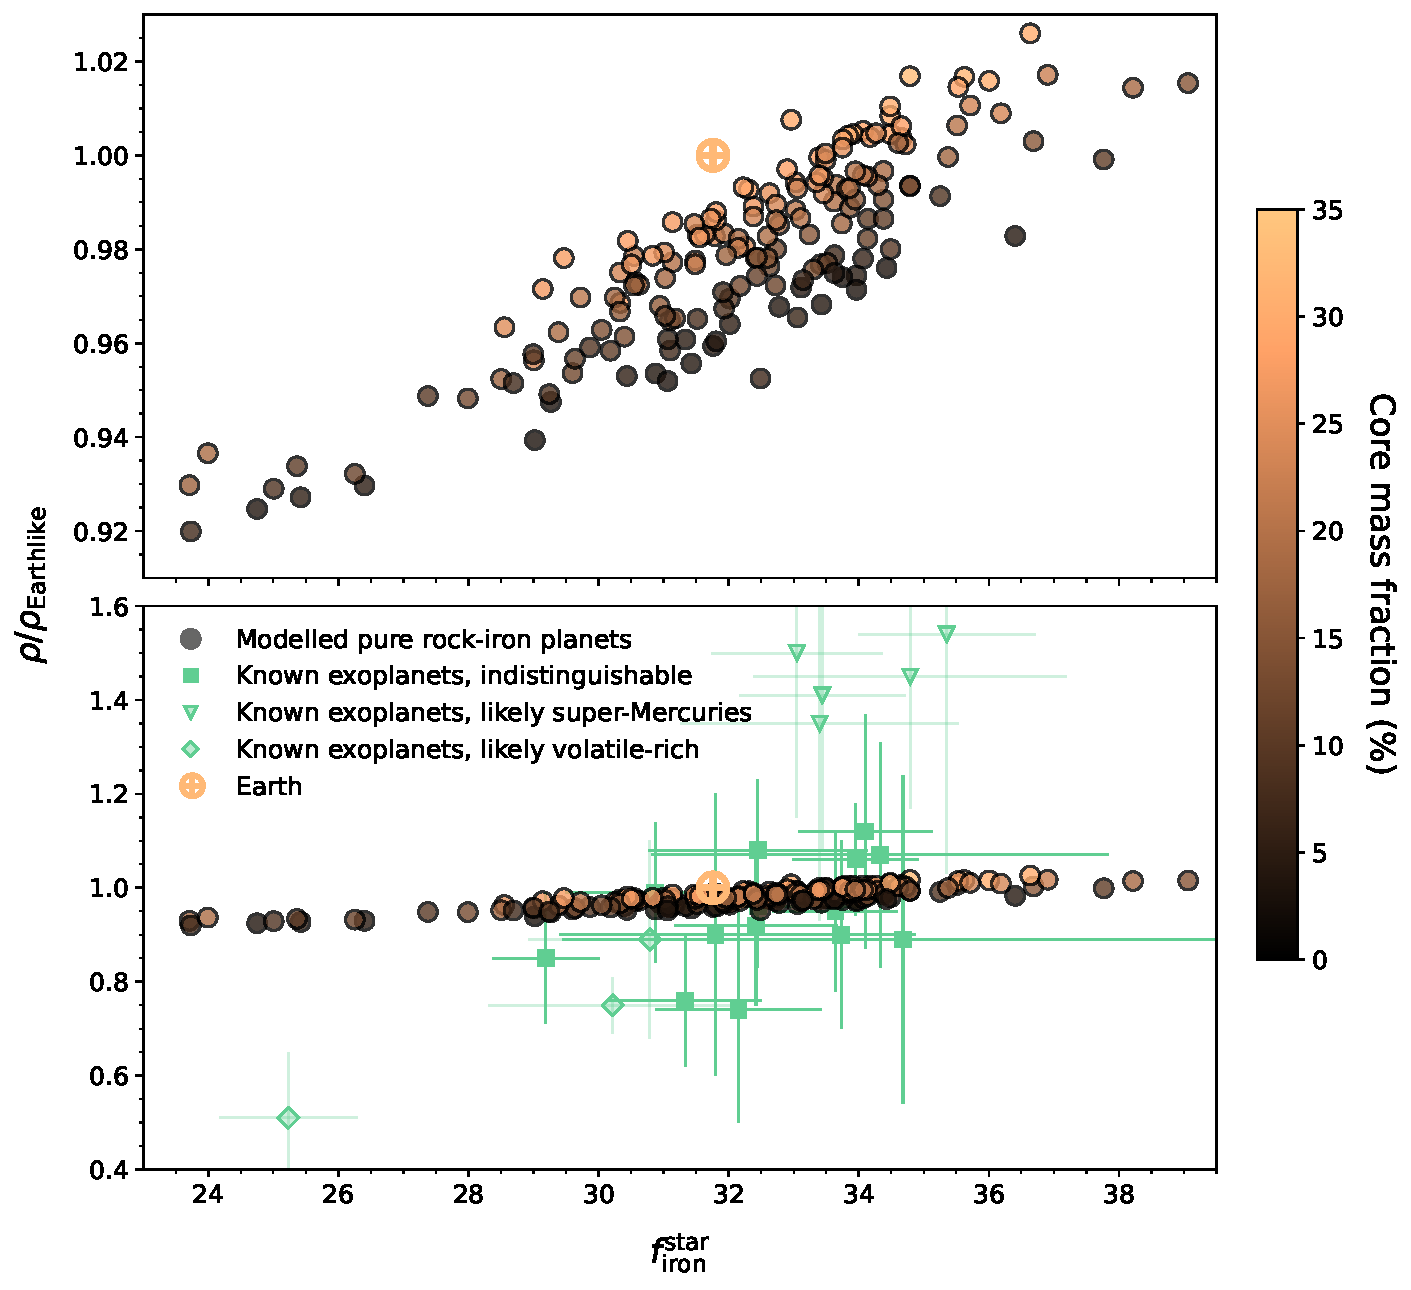
\includegraphics[width=\linewidth]{starplanet_stoich_subplot}
\caption[Test of the link between a planet's bulk density and host star iron abundance, quantifying the intrinsic bulk density scatter due to geochemistry.]{Test of the link between a planet's bulk density and host star iron abundance, quantifying the intrinsic bulk density scatter due to geochemistry \citep[cf.][Fig. 2]{adibekyan_compositional_2021}. The $y$-axis quantity $\rho / \rho_{\rm Earthlike}$ is the bulk density of the planet, scaled to the bulk density of a planet compositionally-identical to Earth. The $x$-axis quantity $f_{\rm iron}^{\rm star}$ is the wt.\% abundance of Fe in the bulk planet calculated from the host star abundances only, using the same stoichiometric method as \citet{adibekyan_compositional_2021} for consistency. Circles show the estimated bulk densities of synthetic Earth-mass planets ($N = 200$) with bulk compositions constrained by observed stellar refractory element abundances for a random sample of planet-hosting stars in the Hypatia Catalog. The synthetic planets have self-consistent mineralogy and density profiles, but ignore that iron cores could have liquid outer layers and/or contain light elements, which would change bulk densities by a few percent (a full description of the interior model is found in Chapter \ref{chapter:rockywater}). Earth's true bulk density is marked with a $\oplus$ symbol. For each modelled planet, the molar fraction of the total iron in its metal core is drawn from a random uniform prior distribition, $\mathcal{U}(0, 1)$, representing hard upper and lower intrinsic geochemical limits to core mass fraction, but not accounting for exogenous processes during planetary formation (e.g., collisional stripping of the mantle, which may have produced Mercury's core mass fraction of 0.7). The modelled core mass fractions (shown by the colourbar), and the modulations of $\rho / \rho_{\rm Earthlike}$ that result, are thus a function of the random Fe partitioning and the constrained stellar iron content. Green markers show the observed exoplanets from \citet{adibekyan_compositional_2021} sample, with triangles denoting the planets they identify as ``super-Mercuries'' (i.e., super-stellar iron core size), and the diamonds denoting the planets from this sample which \citet{unterborn_nominal_2023} identify as likely volatile-rich. The apparent positive correlation between $\rho / \rho_{\rm Earthlike}$ and $f_{\rm iron}^{\rm star}$ has been previously presented as evidence for a compositional link between planets and host stars in \citet{adibekyan_compositional_2021}. From the comparatively shallow slope of this correlation for the hypothetical pure rock-iron planets, after considering possible intrinsic variations in the extent of core formation, it appears that any perceived steeper slope cannot be explained by variations in stellar refractory abundances themselves.}
\label{fig:compositional-link} 
\end{figure}
%\todo{[TODO: show updated TOI-561 b density? scale to solar instead of observed Earth-density, needs recalculating scaled densities for the exoplanets. x-axis uncertainty?]}
% change f_iron_star method, show updated TOI-561 b density, maybe re-calculate scaled density with ExoPlex (better)?
% maybe scale to solar instead of observed Earth-density, needs recalculating scaled density




Figure \ref{fig:compositional-link} shows the exoplanet sample from \citet{adibekyan_compositional_2021}, on the same axes as their Fig. 2, but overlain by hypothetical pure metal-rock planets which I generated to have thermodynamically-consistent mineralogy based on observed stellar abundances \citep{hinkel_stellar_2014}, but with randomly assigned iron partitioning, $X_{\ce{Fe}}^{\rm metal}/(X_{\ce{Fe}}^{\rm metal} + X_{\ce{FeO}}^{\rm silicate})$, uniform between 0 and 1. It appears that the slope between the observed planet bulk density and the host star iron content is steeper than that which would be caused \textit{only} by stellar abudance variations with an unknown extent of core formation. Further, when compared to the synthetic planets, many of the exoplanets in this sample may be less dense than even a coreless planet, if their total iron content is otherwise constrained by the host star composition. These low densities would seem to require the presence of something else: high-molecular-mass atmospheres \citep{schulze_probability_2020}, deep water/steam layers \citep{kite_water_2021}, or magma oceans \citep{bower_linking_2019}. Therefore, the observed exoplanet bulk density variations would not be explained by stellar abundances alone. If the planet-star correlation, it is reported in \citet{adibekyan_compositional_2021}, is real, then we would need an explanation for why its slope is much greater than expected from mineralogy. If we cannot find such an explanation, then this particular correlation might be chance, or poor statistics. As such, it will be important to confirm how small planet volatile budgets relate to the iron abundance of their host star. %Whilst we might expect some sort of continuum of volatile layer thicknesses, very small mass fractions of water (much less than 1 wt.\%) can ensure a planet has no bare land surface, as I will show in Chapter \ref{chapter:topography}.

Nevertheless, \citet{schulze_probability_2020} and \citet{unterborn_nominal_2023} make the important point that the measurement uncertainty on both stellar abundance and planet bulk densities remains mostly too high to distinguish a volatile-enriched planet from an anemic one. High-precision observations of small planets around the most metal-poor, galactic thick-disc stars may be very useful to this end, statistically-speaking \citep[e.g.,][]{brinkman_toi561_2023}. An influence of orbital distances on planetary iron contents is also not strictly ruled out: \citet{mcdonough_terrestrial_2021} report an empirical correlation between the uncompressed densities of solar system bodies with their (current) heliocentric distance, and suggest this to be an effect of the Sun's magnetic field on these bodies' final Fe-metal contents. Whether the quoted effect is robust is not yet testable with observations of exoplanetary systems, however. It may be too early yet to attempt strong conclusions about a link between stellar iron content and planet composition, but we can anticipate improved measurement uncertainty and certainly a multiplying sample size in the near future.
% don't really trust adibekyan "f_iron^star" stoichiometry because it doesn't account for lower mantle being bridgmanite, kind of confusing, not sure if you should try to recreate it or just do in terms of refractory elements
% so far seems like oxidation state doesn't matter, scatter is negligible considering uncertainty, any trend therefore would to be volatiles / light element layers and can't be just from iron content
 
% not varying Si in core but mention how much bulk density difference this would make, also liquid outer core...
% verify with unterborn 2023 nominal range of bulk density - that paper agrees CMF does not have a large effect on bulk density even more so because liquid iron core is more compressible than the mantle. just looking at stellar iron content
% schulz paper's point is that measurement uncertainty too high to be certain that star inferred iron fraction is different than planet bulk density



%Notably, one planet in the \citet{adibekyan_compositional_2021} sample (TOI-561 b) has both anomalously low bulk density and low host-star Fe content---TOI-561 being a metal-poor star in the galactic thick disc. Adding more rocky planets around significantly metal-poor stars to this plot might reveal a clear association between extreme variations in stellar iron content and planet bulk density. However, as it stands, the data point from TOI-561 b would seem to carry disproportional weight in the linear regression, and it would be interesting to see if there is still a statistically significant correlation for thin disc stars only (which vary in Fe abundance by just a few percent). %From Schultze et al it might be pointed out that even if we can't reject the fact that planet core size is not directly related to star iron within the uncertainty, doesn't automatically mean they are predictable. 

%One point seem clear, which is that if we pretend planets are pure iron cores and pure \ce{MgSiO3} mantles, then the empirical core (= iron) mass fractions inferred from bulk density show a broader distribution than the emprical iron mass fractions implied by stellar Fe/(Mg + Si) \citep{plotnykov_chemical_2020}. Therefore, other processes are operating to set planets' core sizes, at the level of accretion, differentiation, or both. More precisely-measured planets in this size regime may give us a better idea of whether this star-planet correlation indeed exists and provides meaningful information on core sizes.





I think it is also worth revisiting here a study by \citet{doyle_oxygen_2019}, measuring FeO abundances in polluted white dwarfs, which is often cited as empirical evidence that most rocky planets have similar $X_{\ce{Fe}}^{\rm metal}/X_{\ce{FeO}}^{\rm silicate}$ to Earth (i.e., equilibrium \eqref{eq:background-iw} is at the same position). Yet insofar as the observed instantaneous pollutant composition does not represent an entire parent body \citep[e.g.,][]{brouwers_asynchronous_2022, brouwers_asynchronous_2023}, the parent body's total iron budget is unknown, and whilst we might be estimating $X_{\ce{FeO}}^{\rm silicate}$ we cannot constrain the iron partitioning from these observations alone. Hence \citet{doyle_oxygen_2019} must assume an Earth-like $X_{\ce{Fe}}^{\rm metal}$. This problem is in addition to the sometimes-unappreciated difficulty in accurately measuring O abundances in polluted white dwarfs (section \ref{sec:background-pwd}). 


To reiterate, the relative iron core sizes of planets are a crucial and poorly-constrained aspect of their characterisation and evolution. I have introduced three reasons why (but there are more). Firstly, because the core radius controls the mantle depth ($d$ in equation (\ref{eq:Ra-background})), it can be just as important as the planet radius in determining the vigour of convection---one of the key parameters governing planets' thermal histories---hence their volcanism, tectonics, and volatile cycling. Secondly, core Fe-metal trades off with mantle Fe oxide, such that for the same bulk Fe inventory, smaller cores imply more FeO in the mantle, which, on top of lowering its viscosity \citep{zhao_effect_2009}, also increases melt productivity \citep{hirschmann_mantle_2000, kiefer_effects_2015}, thickening the juvenile crust that forms from partial melting of this mantle \citep{wade_divergent_2017, dyck_effect_2021}---the consequentially greater volume of hydrous crustal minerals may have contributed to the loss of surface water on Mars \citep{wade_divergent_2017}. Thirdly, estimating the the likelihood of an observed planet being rocky, based on its bulk density and host star abundances, requires an informative prior distribution of core mass fraction. %Although a slighly larger or smaller core may not affect a planet's observed density, it will certainly affect its overall evolution.
This thesis does not aim to make progress towards constraining rocky planet core sizes; nevertheless, it is important to introduce as a limiting problem shared by many exoplanet scientists, from the Earth-up to the space-down. 





%\todo{theory directions: core/silicate mass ratio is set by redox conditions during core formation through equilibria, and a priori we can't say if we expect these to be broadly similar across most rocky planets, therefore CMF not predictable from first principles. Further, core size directly relates to thermal history through affecting the mantle depth, thus having a similar direct consequence as planet mass (eq. Ra); it also relates to mantle iron oxide content which can have far-reaching implications e.g. the the thickness and density of a crust that forms (wade, dyck).}




\section{A big weird universe}

%\todo{e.g, tidal locking, stellar energy distributions, orbital configurations (ellipticity)...Impossible to cover all of these in a study or six... we mention these to avoid upsetting anyone who has a favourite piece of planetary diversity that they have dedicated themselves to the research of, because probably all of this is equally important.---note these things are not internal planet effects so maybe don't even need to mention} 

%Intelligent life capable of observing the solar system would probably think that our terrestrial planets are just as strange.

Despite this thesis' narrative of general trends in prototypical planets, the universe does not make astronomical objects that are all identical save some parameter. Real planets have idiosyncracy. Many of the known rocky worlds, so far the easiest for us to detect, orbit so close to their stars as to be tidally-locked: with a permanent day side and night side, like the Moon is to Earth. Simulations of mantle convection on tidally-locked planets have shown the extreme hemispheric contrast in surface temperature could influence their mantle convection \citep{vansummeren_mantle_2011, gelman_effects_2011, meier_hemispheric_2021}---in stark contrast to the planets discussed here, where stellar radiation has no effect on interior evolution. Some of these worlds, like CoRoT-7 b and 55 Cancri e, are kept so exceedingly hot that they may remain molten for billions of years, never crystallising a mantle \citep{leger_transiting_2009, demory_map_2016}. Other internal heating mechanisms could operate on short-period exoplanets, namely tidal dissipation \citep{driscoll_tidal_2015, renaud_increased_2018, dobos_tidal_2019} and induction heating by the stellar magnetic field \citep{kislyakova_electromagnetic_2020, grayver_interior_2022}. Of course interior convection is just as holistically important on these planets, but it will be in a different regime; ``generalised" thermal evolutions cannot be extrapolated across different regimes of convection, as I have stressed. Magnetic fields and their consequences are not addressed here, although they are a direct outcome of thermal evolution and so convection models have been used to predict their likelihoods \citep{nimmo_why_2002, gaidos_thermodynamic_2010, driscoll_thermal_2014, Foley2016, boujibar_superearth_2020, zhang_thermal_2022}. Also influencing a planet's surface, of course, are the astrophysical factors: non-circular orbits \citep{williams_earthlike_2002, dobrovolskis_spin_2007, way_effects_2017, palubski_habitability_2020}, for example, or the spectral energy distribution of the host star \citep{kasting_ultraviolet_1997, shields_effect_2013, godolt_3d_2015, eager-nash_implications_2020}, all getting their dedicated attention elsewhere. It is impossible to %cover everyone's favourite aspect of exoplanet diversity, 
cover every factor causing rocky planets to diverge, but this chapter has covered what I believe to be the most salient ones.
% Throughout this section I have explained the assumptions and simplifications that make planetary interior models tractable.

% moons, but moonless earth probably not uninhabitable latest simulations

% .magnetic fields seem relevant for UV shielding and atmospheric stripping \citep{dong_atmospheric_2020}, but is clearly not the only thing comparing Venus to Earth , and may not be a sufficient condition \citep{gunell_why_2018}




\section{Structure of the thesis}



This thesis combines foundational planetary science, state-of-the-art numerical tools, and nimble box-model insights to investigate several cases of rocky planet diversity from the inside out. In doing so, I make some contribution towards several core research questions:

\begin{itemize}

\item How easily is surface topography generated on planets?
\item To what extent do stagnant lid planets cycle their volatiles between interior and surface?
\item Does stellar chemistry influence the volatile composition of planetary mantles, their magmas, and their derived volcanic gases?

\end{itemize}


\textbf{Chapter \ref{chapter:topography}} estimates the heights of intrinsic topography on rocky planets which is a basic consequence of their mantle convection. Topography carves out basins to contain surface water, so planets with higher topography would be more prone to having islands above sea level. \textbf{Chapter \ref{chapter:outgassing}} then applies a mantle convection model to pre-plate tectonics Archean Earth, questioning the contemporaneous high rates of volcanic outgassing inferred when classic thermal history models \citep[e.g.,][]{schubert_whole_1980} are extrapolated backwards in time. Archean Earth presents a useful case study to explore in-depth with justifiably more-sophisticated numerical models. %, such as the one here coupling convection with melting and redox chemistry. 
\textbf{Chapter \ref{chapter:rockywater}}, recognising that exoplanets' initial interior water contents have never been constrained---but are a principle factor affecting water outgassing rates (from Chapter \ref{chapter:outgassing})---predicts the maximum water that would be stored in mantle minerals across the expected range of bulk compositions. Lastly, in \textbf{Chapter \ref{chapter:fo2}}, I show that there must be at least a multiple-order-of-magnitude variation in how oxidising these mantles will be across the same range in bulk composition. Given that small changes in redox conditions can have large consequences for petrological and atmospheric evolution on planets, these last results emphasise even more how modern Earth represents a specific outcome of thermal-chemical-geodynamic evolution; planet Earth is fading as the old cosmic modality. \textbf{Chapter \ref{chapter:conclusion}} synthesises this work under the loose theme of water and life on rocky worlds. 


%!TEX root = ../thesis.tex
%*******************************************************************************
%*********************************** First Chapter *****************************
%*******************************************************************************

\chapter{Blue marble, stagnant lid: Could dynamic topography avert a waterworld?}  %Title of the First Chapter
\label{chapter:topography}

\ifpdf
    \graphicspath{{Chapter1/Figs/Raster/}{Chapter1/Figs/PDF/}{Chapter1/Figs/}}
\else
    \graphicspath{{Chapter1/Figs/Vector/}{Chapter1/Figs/}}
\fi

\section*{Preface}

This chapter was published under the same title in \textit{The Planetary Science Journal} in March 2022, appearing in the bibliography as \citet*{guimond_blue_2022}. After a short note on author contributions, it is presented here reformatted but otherwise unchanged. 


\subsubsection*{Contributions and context}

I acknowledge John Rudge and Oliver Shorttle, who coauthored the published version of this article. It was Oli's idea to model how high topography can be on exoplanets. We developed this idea into a PhD research proposal in late 2018 (which then ended up securing me a funded position). John crucially lent his expertise as I worked out the mantle convection modelling aspects of the study during the fist year and a half of my PhD, guided me through some of the more arcane maths (spherical harmonics!), and prompted much of the focus on scaling laws. Both have provided insightful comments and editorial input. This article has undergone peer review. %I also acknowledge two anonymous reviewers, whose feedback is reflected in version you see here.

\section*{Abstract}

Topography on a wet rocky exoplanet could raise land above its sea level. Although land elevation is the product of many complex processes, the large-scale topographic features on any geodynamically-active planet are the expression of the convecting mantle beneath the surface. This so-called ``dynamic topography'' exists regardless of a planet's tectonic regime or volcanism; its amplitude, with a few assumptions, can be estimated via numerical simulations of convection as a function of the mantle Rayleigh number. We develop new scaling relationships for dynamic topography on stagnant lid planets using 2D convection models with temperature-dependent viscosity. These scalings are applied to 1D thermal history models to explore how dynamic topography varies with exoplanetary observables over a wide parameter space. Dynamic topography amplitudes are converted to an ocean basin capacity, the minimum water volume required to flood the entire surface. Basin capacity increases less steeply with planet mass than does the amount of water itself, assuming a water inventory that is a constant planetary mass fraction. We find that dynamically-supported topography alone could be sufficient to maintain subaerial land on Earth-size stagnant lid planets with surface water inventories of up to approximately $10^{-4}$ times their mass, in the most favourable thermal states. By considering only dynamic topography, which has $\sim$1-km amplitudes on Earth, these results represent a lower limit to the true ocean basin capacity. Our work indicates that deterministic geophysical modelling could inform the variability of land propensity on low-mass planets.



\section{Introduction}

The concurrence of land and water on a planet's surface will affect its climate state \citep{turbet_habitability_2016, rushby_effect_2019, delgenio_albedos_2019, graham_thermodynamic_2020, zhao_climate_2021}, the planetary context of potential biosignatures \citep{schwieterman_exoplanet_2018, glaser_detectability_2020, lisse_geologically_2020, krissansen-totton_oxygen_2021}, and perhaps its likelihood to host the prebiotic chemistry that leads to the origin of life \citep{patel_common_2015, rimmer_origin_2018, rosas_archaean_2021, vankranendonk_elements_2021}. Planets with no exposed land area, and only a liquid layer at the surface-atmosphere interface, would follow different patterns of chemical and heat transfer compared to modern Earth---one consequential open question is whether a silicate weathering feedback could efficiently regulate the climate on such planets \citep[e.g.,][]{honing_carbon_2019, gernon_global_2021}. Although these ocean planets certainly remain important targets for understanding exoplanetary diversity, there are indications that they are incompatible with some origins-of-life scenarios, specifically with regards to the hydrolysis of polymers, attenuation of necessary UV radiation, and possibly lower availability of crust-weathered P that all occur in the deep ocean \citep[e.g.,][]{sutherland_opinion_2017, walton_phosphorus_2023}. The likelihood that a given exoplanet is hospitable to life as we know it may therefore be related to the likelihood that the planet has both land and surface water.


Planetary land/ocean fractions emerge in a compromise between water's total budget and distribution between surface and interior reservoirs, and the size of the basins carved out by topography \citep[e.g.,][]{simpson_bayesian_2017}. The resulting ocean mass from the former is largely stochastic: coded within it are the histories of volatile delivery during accretion \citep{raymond_highresolution_2006, morbidelli_building_2012}, interior degassing from the magma ocean and succeeding mantle \citep{elkins-tanton_linked_2008, schaefer_redox_2017,  katyal_effect_2020, ortenzi_mantle_2020, guimond_low_2021, barth_magma_2021, lichtenberg_vertically_2021, bower_retention_2021}, atmospheric erosion by impacts \citep{zahnle_cosmic_2017, schlichting_atmosphere_2018, howe_survival_2020}, and photodissociative atmospheric escape \citep{tian_water_2015, zahnle_strange_2019, gronoff_atmospheric_2020}, along with the surface temperature and pressure. In contrast, large-scale aspects of planetary topography may lend themselves to deterministic relationships with observable planetary bulk properties. Although substantial water budgets of a few wt.\% would inevitably produce waterworlds \citep[e.g.,][]{simpson_bayesian_2017}, at smaller water mass fractions the outcome is sensitive to the planet's topography; even a tiny ocean mass would inundate an atopographic body. Early constraints on exoplanet land propensity might therefore start with topography.

% more details are required to explain to the reader why you are trying to avoid waterworlds



This first investigation will limit itself to forms of topography that could exist without moving plates. Whether or not a given planet manifests plate tectonics appears to be hysteretic and largely unanswerable by modelling from state variables \citep{lenardic_notion_2012, weller_evolution_2018, lenardic_diversity_2018}. Consequentially, this paper adopts the working hypothesis that a stagnant lid describes a temperate rocky planet's most natural regime \citep{stern_stagnant_2018}. Here the cool outermost rock layer does not experience enough stress to trigger its breaking into plates by brittle failure.

%While \citet{meier_hemispheric_2021} have recently proposed a mobile-lid scenario for the ultra-short-period planet LHS 3844b using constraints from thermal phase curve observations, this may be interpreted as a special case associated with this planet's extreme hemispheric temperature contrast.
% Indeed, laboratory experiments and numerical models show...

Of the types of topography on planets, so-called dynamic topography---the surface deformation from convective upwellings and downwellings in the mantle---can create significant elevation differences without requiring plate tectonics. Although dynamic topography is not independent of plate movement on Earth, where mantle convection beneath divergent and convergent plate boundaries has built ridges higher than sea level and trenches deeper than Mount Everest, respectively, and though we expect dynamic topography to be muted in the absence of plate tectonics, mantle convection would retain an inevitable influence on the low-order shape of the stagnant lid surface. That is, dynamic topography is everywhere: a planet exhibits this phenomenon so long as its interior convects. Bodies in our solar system do boast high peaks by other means: massive lava flows (e.g., Olympus Mons) or impact cratering (e.g., Rheasilvia on Vesta). Yet if we are interested in whether a planet's topography could be higher than its sea level \emph{regardless of} volcanism, cratering, and other processes contingent on a planet's specific geological history, then we might begin with dynamic topography as the most endogenously universal of relief mechanisms. 


On long length scales of relief, additional support comes from the density contrast between the heavier mantle and lighter crust, which buoys topography at an equilibrium height. This isostatically-compensated topography can be higher in part because the maximum stress underneath the load is shifted to shallower, cooler depths, where the lithosphere is stronger. Parameterisations of isostatic equilibria, however, depend only on the density contrast and thickness of the crust, and so are sensitive to the planet's specific petrologic history. This could be daunting if we consider that the emergence of thick granitic continents on Earth still lacks a consistent explanation, but is probably entwined with its geodynamic history \citep{lenardic_continental_2005,
korenaga_crustal_2018, honing_bifurcation_2019}. Predicting isostatic elevations would require information which may always be model-dependent. Purely dynamic topography, meanwhile, both originates from and is supported by the sole process of thermal convection. It is directly obtained from any numerical convection model \citep[e.g.,][]{mckenzie_surface_1977, kiefer_geoid_1992, kiefer_geoid_1998, huang_constraints_2013, arnould_scales_2018, lees_gravity_2020}; its prediction requires less prior knowledge.

Note that stagnant lid convection can lead to other forms of topography, beyond just that supported dynamically by convection (Fig. \ref{fig:topography-schematic}). The melting associated with hot upwelling mantle can form thick, low-density crust as in Fig. \ref{fig:topography-schematic}d \citep{stofan_large_1995}; further, tension above downwelling plumes can also thicken the crust tectonically as in Fig. \ref{fig:topography-schematic}b \citep{kiefer_mantle_1991,pysklywec_timedependent_2003, zampa_evidence_2018}. Both phenomena would induce compositional isostasy, resulting in altitudes unrepresentative of pure dynamic support. Neither, however, will be included in the groundwork we perform here. There is also a distinction to be made for \textit{thermal} isostasy, in which thermal expansion of the lithospheric mantle creates the density difference, rather than compositional separation related to melting (Fig. \ref{fig:topography-schematic}c). Hot upwelling mantle will induce thermal isostasy. By convention, we do include thermal isostasy within the full dynamic topography \citep[see][]{molnar_mantle_2015, hoggard_observational_2021}. Overall, the elevations we model here should represent conservative lower limits on a stagnant lid planet's static topography.

\begin{figure*}
  \centering
  \begin{subfigure}[b]{0.5\textwidth}
    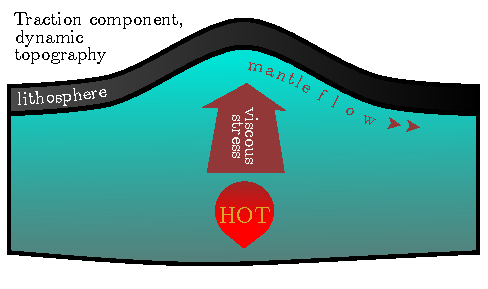
\includegraphics[width=\textwidth]{schematic-a.pdf}
    \caption{}
    \label{fig:schematic-a}   
  \end{subfigure}  
  \hfill           
  \begin{subfigure}[b]{0.5\textwidth}
    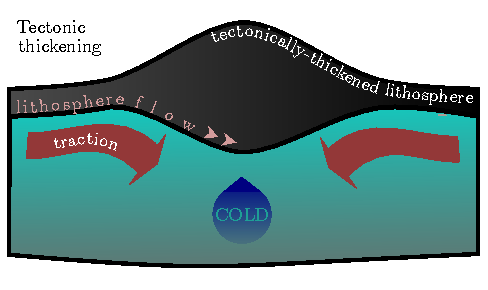
\includegraphics[width=\textwidth]{schematic-b.pdf}
    \caption{}
    \label{fig:schematic-b}
  \end{subfigure}     %
           
  \begin{subfigure}[b]{0.5\textwidth}
    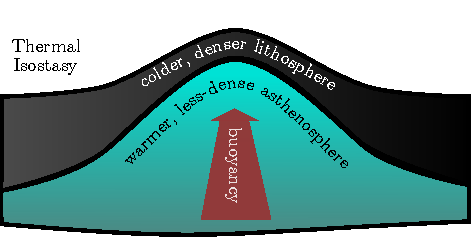
\includegraphics[width=\textwidth]{schematic-c.pdf}
    \caption{}
    \label{fig:schematic-c}
  \end{subfigure}
  \hfill
    \begin{subfigure}[b]{0.5\textwidth}
    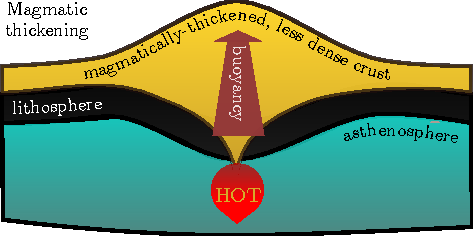
\includegraphics[width=\textwidth]{schematic-d.pdf}
    \caption{}
    \label{fig:schematic-d}
  \end{subfigure}
  \caption[The four major endogenic sources of topography on a stagnant lid planet.]{The four major endogenic sources of topography on a stagnant lid planet. \textit{(a)} The component of dynamic topography due to flow-induced traction on the lithosphere. \textit{(b)} Tectonic crustal thickening caused by tension over cold downwellings. \textit{(c)} The component of dynamic topography due to thermal isostasy over thinned lithosphere. \textit{(d)} Magmatic crustal thickening caused by melting of upwelling plumes.}
  \label{fig:topography-schematic}
\end{figure*}




In summary, among the large-scale mechanisms sculpting the surface of an active planet, dynamic topography alone has the advantage of being (i) inevitably present, regardless of tectonic mode; and (ii) a direct result, quantitatively, of a tractable process (mantle convection). From a modelling perspective, all of these factors help define a simplified and tractable problem: how does dynamic topography scale with parameters that dictate how a planet will convect---like the depth of the mantle, the thermal state, or the rheology? In principle this scaling relationship can be extracted from numerical simulations of convection. From there, cheaper 1D parameterised convection models can use this scaling to explore how the amplitude of dynamic topography changes over a wide range of planetary bulk properties. Because the scaling itself may be sensitive to a planet's tectonic mode, our convection simulations neglect the possibility of plates.

\subsection{Dynamic topography scaling relationships}\label{sec:intro-scaling}

Limited by computing power, early constructions of a scaling function for dynamic topography have used a constant viscosity for the convecting region \citep{parsons_relationship_1983, kiefer_geoid_1992}. Under this isoviscous paradigm, a single dimensionless parameter, the Rayleigh number, describes the convective vigour of the system:
\begin{equation}\label{eq:Ra}
    {\rm Ra} = \frac{\alpha\rho g \Delta T d^3}{\kappa \eta},
\end{equation}
\nomenclature[g-a]{$\alpha$}{thermal expansivity [K$^{-1}$]}
\nomenclature[g-p]{$\rho$}{density [${\rm kg\,m^{-3}}$]}
\nomenclature[a-g]{$g$}{acceleration due to gravity [${\rm m\,s^{-2}}$]}
%\nomenclature[a-tempx]{$\Delta T$}{temperature contrast [K]}
\nomenclature[a-d]{$d$}{thickness of convecting layer in Rayleigh number calculation [m]}
\nomenclature[g-k]{$\kappa$}{thermal diffusivity [${\rm m^2\,s^{-1}}$]}
\nomenclature[g-e]{$\eta$}{dynamic viscosity [${\rm Pa\,s}$]}
where $\alpha$ is the thermal expansivity of the material in K$^{-1}$, $\rho$ is its density in ${\rm kg\,m^{-3}}$, $g$ is the surface gravity in ${\rm m\,s^{-2}}$, $\Delta T$ is the temperature contrast across the layer in K, $d$ is the depth of the convecting region in m, $\kappa$ is the thermal diffusivity in ${\rm m^2\,s^{-1}}$, and $\eta$ is the dynamic viscosity in Pa~s---in isoviscous convection these parameters are all constant. The Ra number can act as a useful independent scaling variable for many convection phenomena because the vast majority of temperature variations in a convecting cell occur in its boundary layers \citep{mckenzie_convection_1974}. Boundary layer theory justifies a power-law relationship between Ra and the thickness of the upper thermal boundary layer. Hence these previous works on isoviscous dynamic topography supposed scaling relationships of the form $h/(\alpha \Delta T d) \sim {\rm Ra}^n$ (the $\alpha \Delta T d$ term ensures that both sides of the proportionality are dimensionless and $n$ is uniquely defined). %Power law functional forms are preferred for such systems where scaling behaviour is best seen in magnitudes, and the data from numerical experiments cannot justify something more complex than a log-linear model. \jr{I'm not keen on this paragraph. In an isoviscous problem, everything can be reduced by scaling to be a function of the Rayleigh number, whether that be topography or boundary layer thicknesses. Moreover, the main temperature variations are not limited to the upper boundary layer -- they're in the other boundary layers too, including the rising and sinking plumes. I also think stress variations are broadly distributed across the layer for an isoviscous flow. I'd give an older isoviscous reference for the boundary layer scaling (e.g. McKenzie 1974 JFM), as you haven't introduced T-dep viscosity yet. I don't understand what you mean by the "power-law functional forms are preferred" sentence -- as you say, the power-law functional forms for the isoviscous cases can be justified by boundary layer theory here.}

In rocky planets, however, $\eta$ changes with temperature \citep{karato_rheology_1993}; steep viscosity gradients across the mantle are a defining trait of natural stagnant lid convection in that the cold surface is too viscous to flow \citep{davaille_transient_1993, solomatov_scaling_1995}. Scalings based on (\ref{eq:Ra}) defined using constant viscosity will not necessarily provide an optimal fit to the topography of stagnant lid bodies \citep{sembroni_impact_2017, bodur_impact_2019}. In identifying a convecting system whose viscosity decreases quickly with temperature, we need a second dimensionless parameter in addition to a Rayleigh number: the viscosity contrast across the layer, $\Delta \eta=\eta_0/\eta_1$, where $\eta_0$ is the viscosity at the top and $\eta_1$ the viscosity at the bottom. A nonuniform viscosity profile implies many possible thermal Rayleigh numbers. Here Ra$_1$ denotes (\ref{eq:Ra}) evaluated at $\eta=\eta_1$. In simple numerical models, viscosity is often assumed to follow an exponential law, $\eta(T) = \eta_0 \, {\rm exp}(-b T)$, where the temperature prefactor $b = \ln\left(\Delta \eta\right)$ is a constant \citep{solomatov_scaling_1995}. 
\nomenclature[a-rayleigh]{Ra}{thermal Rayleigh number}  
\nomenclature[g-e]{$\Delta \eta$}{dynamic viscosity ratio between top and bottom of convecting layer}  
\nomenclature[a-b]{$b$}{temperature prefactor in dimensionless exponential viscosity law}  
%\nomenclature[s-0]{$0$}{value at top of convecting layer}                    % first letter S is for subscripts
%\nomenclature[s-1]{$1$}{value at bottom of convective layer}                    % first letter S is for subscripts

Further, any Ra scaling function will only apply to its intended convection regime. Canonical studies of temperature-dependent viscosity convection distinguish between at least two series of regimes. These regimes have their own transitions in Ra$_1$-$\Delta \eta$ space, which would manifest as discontinuities in the scaling function. %, wherein the value of the power-law exponent changes.\jr{I wouldn't presume a power-law scaling of dynamic topography -- your data suggests it is not a simple power-law relation (although we are going to approximate as so).} 
A first series concerns the mobility of the surface: as $\Delta \eta$ increases, a convecting system will move from a small viscosity contrast regime (similar to the isoviscous case) to a stagnant lid regime, via an intermediate regime of a sluggish lid \citep{solomatov_scaling_1995, moresi_numerical_1995, kameyama_transitions_2000}. In a second series of transitions, the so-called stationarity of convection changes. As Ra$_1$ increases, the system will move roughly from a steady-state regime to a chaotic time-dependent regime, again through a transitional regime \citep{dumoulin_heat_1999, solomatov_scaling_2000}. For either series, the regime boundaries are not sharp in Ra$_1$-$\Delta \eta$ space, but depend on this parameter space in a complex way via the aspect ratio of convection and the initial conditions. Whilst ascribing Ra$_1$ presumes a bottom-heated convection cell, different modes of heating may also affect dynamic topography scaling relationships in ways we do not yet understand. 

A waypoint objective of this work is therefore to develop a preliminary dynamic topography scaling relationship for the stagnant lid regime. Whilst the topography of  stagnant lid bodies has indeed been modelled numerically before \citep{moresi_interpreting_1995, solomatov_stagnant_1996, vezolainen_timing_2003, vezolainen_uplift_2004, orth_isostatic_2011, golle_topography_2012, huang_constraints_2013}, the majority of this literature is directed at producing geoid-to-topography ratios to invert for interior properties of Venus or Mars, as opposed to fully exploring parameter space with forward models. As such, we are aware of no published scalings as explicit functions of the relevant convective parameters. Given the scope of our work here, we do not attempt to characterise the scaling behaviour near the regime discontinuities (which would require a much finer grid of models in Ra$_1$-$\Delta \eta$ space). Instead, we restrict ourselves to the chaotic time-dependent stagnant lid regime located in \citet{moresi_numerical_1995} and \citet{orth_isostatic_2011}, and simulated previously with Venus- and Mars-like parameters \citep{solomatov_scaling_2000, hauck_thermal_2002, reese_scaling_2005, orth_isostatic_2011}. As such, we are assuming that chaotic stagnant lid convection will apply to most geodynamically-active rocky planets---an assumption that may be tested in the future when detailed characterisation of rocky exoplanets becomes possible.
%\footnote{As an alternative to the scaling relationships explored here, \citet{orth_isostatic_2011} present an ``isostatic stagnant lid approximation" to dynamic topography, on the basis that thermal isostasy is by far the most impressive contributor to the surface dynamic topography (cf. the viscous stress itself). However, their approximation requires knowing how surface temperature varies in two dimensions, and hence cannot be applied to 1D parameterized convection models as we are wont to do.}




%   # The viscosity is defined as \[\eta = \text{Di} / \text{Ra} \cdot \exp(-b
%   # T' + c z)\] where $T'$ is the temperature variation from the adiabatic
%   # temperature, $z$ is the depth, $b$ is given by ``Viscosity temperature
%   # prefactor'', and $c$ by ``Viscosity depth prefactor''. If $\text{Di}$ is
%   # zero, it will be replaced by 1.0 in $\eta$.
  

\subsection{The harmonic structure of planetary surface relief} \label{sec:intro-spectrum}

In the second part of this study, we convert scaled dynamic topographies into the corresponding volumes of the largest possible ocean basin. The key product here is a spherical harmonic expansion of this scaled topography onto a Cartesian grid, as a synthetic elevation map. Yet, all that our stagnant lid convection scaling law provides is a scalar height value. With some convenient assumptions about dynamic topography's spectral properties, it is in fact straightforward to find a power spectrum which is consistent with both the scalar height we have, and with some set of spherical harmonic coefficients we need.

Initial observations of Venus, Earth, and Mars' (total) topographies suggested a remarkably log-linear relationship between the 1D power spectral density, $\phi^{\rm PSD}_h$ in m$^3$, and the wavenumber, $k$ in m$^{-1}$. From spherical harmonic degree $l=5$ to at least $l=100$, the available spectra appeared consistent with a slope dlog$\phi^{\rm PSD}_h$/dlog$k \sim-$2 \citep{turcotte_fractal_1987, rapp_decay_1989, balmino_spectra_1993}. This precise slope value was predicted earlier still by \citet{vening1951remarkable} and appears to be physically-motivated \citep{sayles_surface_1978, lovejoy_l1_1995}---perhaps emerging from sediment transport laws \citep{pelletier_why_1997, pelletier_selforganization_1999, roberts_generation_2019}, although we will not be considering topography's modification by erosion explicitly. Statistically, a slope of $-$2 corresponds to red noise, the noise associated with a random walk process. 
\nomenclature[g-f]{$\phi^{\rm PSD}_h$}{1D power spectral density of topography [m$^3$]}  
\nomenclature[a-l]{$l$}{spherical harmonic degree}  
\nomenclature[a-k]{$k$}{wavenumber [m$^{-1}$]}                   


%A constant spectral slope would mean that topography is scale-invariant (that is, fractal) in this wavenumber range: the elevation gain measured over some distance $\Delta x$ is proportional to the measuring stick $\Delta x$. 


The convenient consequence of a log-linear spectral model---with a pre-determined slope---is that it would let us approximate the shape of any planetary surface given just one free parameter; i.e., the $y$-intercept of $\phi^{\rm PSD}_h(k)$. %\footnote{Note that on top of a slope and intercept, one must also provide a minimum wavenumber below which $\phi^{\rm PSD}_h(k)$ ``rolls off" to a flat spectrum. In most cases this can be determined from the size of the planet.} 
As for dynamic topography in particular, models and Earth observations have indicated a shallower spectral slope roughly consistent with pink noise $\propto k^{-1}$, up to $l\sim30$ \citep{hoggard_global_2016, hoggard_oceanic_2017, davies_earth_2019}. However, there is no evidence that this spectral structure should characterise dynamic topography under all tectonic regimes. Hence, we extract the spectral structure of our own numerically-modelled stagnant lid topography profiles. We will see that our rudimentary analysis again produces constant dlog$\phi^{\rm PSD}_h$/dlog$k$ values, albeit ones more strongly negative than $-$2. Observations of real stagnant lid bodies in the solar system could then suggest an empirical modification of this purely-dynamic spectral model. 


% \jr{See previous caveats.}

% A constant spectral slope implies that topography is scale-invariant; that is, fractal.\footnote{Note that in fractal parlance, the term ``scale-invariance" has a different meaning from the ``scaling relationships" referred to when discussing convection models.} Such a framework is very convenient for the present work because it lets us statistically describe the surface relief of an entire planet with a small handful of parameters \citep[e.g.,][]{gagnon_multifractal_2006, landais_universal_2015, landais_multifractal_2019}, despite the many complex, multi-scale processes which topography would integrate. 

% \todo{[maybe with all the discussion about red noise topography you should include such a spectrum as a third case study in the ocean basin volume figure (tho I doubt it would look different).]}




% \todo{point is that this result taken into context with the dynamic topography slopes from \citet{hoggard_global_2016} (and others?) might hint at a working hypothesis that geodynamically-active bodies with atmospheres have statistically-consistent topography spectra. An implication of this hypothesis is that if we know the dimensional RMS topography, and we know the spectral slope of the mean, then we have all we need to determine a spherical harmonic power spectrum of dimensional topography for a rocky exoplanet given X bulk properties. From this we can randomly generate elevation maps consistent with the spectrum and do stuff with them...  }

\subsection{Study outline}



% We attempt to start bridging this gap by applying deterministic geophysical models of topography to statistical representations of its scale-invariance. \jr{? I don't understand this. I think all we care about is getting a rough scaling between peak and rms topographies so we can do ocean basin calculations. }


Our methods are described in section \ref{sec:methods}. The approach we take is outlined as follows: we begin by extracting scaling relationships for the RMS amplitude of dynamic topography from 2D numerical mantle convection simulations with temperature-dependent viscosity (section \ref{sec:results-scaling}). Second, we embed these scaling relationships in a suite of 1D parameterised convection models, allowing us to explore the sense of change of RMS dynamic topography across a wide model parameter space and planet age distribution (section \ref{sec:results-parameters}). For this parameter study we focus on the planet mass, age, radiogenic element abundance, and core mass fraction, all relevant to the cooling history and Rayleigh number of a planet. We focus on these four parameters because they may be amenable to being observationally constrained for exoplanets, at least in principle. Third, we synthesise 2D maps from the projected RMS amplitudes to see how the maximum capacity of ocean basins, and hence the minimum elevation gain needed for dry land, might trade off with planet size (section \ref{sec:results-ocean}). We end with a discussion of the study's limitations and applicability (section \ref{sec:discussion-top}).



%%%%%%%%%%%%%%%%%%%%%%%%
\section{Methods} \label{sec:methods}

\subsection{Numerical convection model} \label{sec:methods-numerical}

Numerical computations were performed using the ASPECT code version 2.2.0 \citep{KHB12,heister_high_2017, bangerth_aspect_2020}. For each case we systematically varied two key input parameters: Ra$_1$ and $\Delta \eta$. Although we originally explored Ra$_1$ varying from $1 \times 10^7$ to $3 \times 10^8$, we found that simulations below Ra$_1 = 1 \times 10^8$ were not in the chaotic time-dependent regime, and showed characteristically different topography scaling behaviour. Because the present study was not designed to precisely locate these transitions, we focused only on the chaotic time-dependent regime. Simulations above Ra$_1 = 3 \times 10^8$ were found to be computationally impractical.

Our ASPECT implementation 
% solves the governing equations of convection in their dimensionless forms,
% \begin{align}
%     \begin{split} \label{eq:governing}
%     \nabla \cdot \mathbf{v}^\prime &= 0, \\
%     - \nabla \mathcal{P}^\prime + \nabla^2 \mathbf{v}^\prime &= {\rm Ra} \, \theta^\prime \, \mathbf{\hat{z}}, \\
%     \frac{{\rm D}\theta^\prime}{{\rm D}t^\prime} &= \kappa^\prime \nabla^2 \theta^\prime, \\ 
%     \end{split}
% \end{align}
% where $\mathbf{v}^\prime$ is the dimensionless velocity, $\mathcal{P}^\prime$ is the dimensionless non-hydrostatic pressure, and $\theta^\prime$ is the dimensionless potential temperature. This 
results in dimensionless temperature and velocity fields, denoted by the prime symbol. These and their derivative quantities can be dimensionalised as, e.g.,
\begin{align}
    \begin{split} \label{eq:dimensionalise}
    T &= \Delta T \; T^\prime + T_0, \\
    u &= \frac{\kappa}{d} \; u^\prime, \\
    (x, y) &= d \; (x^\prime, y^\prime), \\
    \delta_{\rm rh} &= d \; \delta_{\rm rh}^\prime, \\
    D_{\rm lid} &= d \; D_{\rm lid}^\prime, \\
    h &= \alpha \Delta T d \; h^\prime,
    \end{split}
\end{align}
\nomenclature[g-d]{$\delta_{\rm rh}$}{thermal boundary layer thickness [m]}  
\nomenclature[a-d]{$D_{\rm lid}$}{stagnant lid thickness [m]}  
\nomenclature[a-u]{$u$}{velocity [${\rm m\,s^{-1}}$]}  
\nomenclature[r-aaaa]{$^\prime$}{nondimensionalised value of parameter}  
where $T^\prime$ is the dimensionless temperature, $u^\prime$ is the horizontal component of the dimensionless velocity, $\delta_{\rm rh}^\prime$ is the dimensionless thickness of the upper thermal boundary layer, $D_{\rm lid}^\prime$ is the dimensionless thickness of the stagnant lid, $h^\prime$ is the dimensionless height of topography, $T_0$ is the dimensional surface temperature, $\Delta T$ is the dimensional temperature difference from bottom to surface, and the other (dimensional) parameters are defined under (\ref{eq:Ra}) above. 

All simulations involve a 2D rectangular box with fixed top and bottom temperatures, $T_0^\prime = 0$ and $T_1^\prime = 1$ respectively, and no internal heating. Free-slip boundary conditions are ascribed to the top and bottom surfaces, whilst reflecting boundary conditions are ascribed to the sides. We use a wide box with a nondimensional depth $Y^\prime$ of unity and a nondimensional width of $X^\prime = 8Y^\prime$ to minimise the influence of the side walls. We assume an incompressible, infinite-Prandtl-number fluid and use the Boussinesq approximation. Viscosity is Newtonian and varies with temperature according to an exponential rheology law, $\eta^\prime = \exp(-b \, T^\prime)$, where $b = \ln (\Delta \eta)$. We use the coarsest mesh size still able to resolve the lower thermal boundary layer; this varies for different Ra$_1$. Table \ref{tab:aspect} lists the relevant details of the model setup.

Each experiment is deemed to have reached quasi-steady-state when both its RMS velocity stabilises to within 0.002\% and its top and bottom heat fluxes converge. All time steps prior to this point are discarded, and the models are then allowed to run for long enough such that the distribution of RMS dynamic topography is well-characterised. All cases are confirmed to be in the stagnant lid mode of convection based on the surface mobility criterion, $S = (\delta_0^\prime)^2 u_0^\prime \ll 1$, where $\delta_0^\prime = D_{\rm lid}^\prime + \delta_{\rm rh}^\prime$ is the dimensionless thickness of the lithosphere, and $u_0^\prime$ is the dimensionless surface velocity \citep{solomatov_three_1997}.

\begin{table}
\centering
\caption{Numerical convection model setup for dynamic topography experiments.\label{tab:aspect}}
\footnotesize
\begin{tabular}{@{} c r r r l @{}}
\toprule
Case & Ra$_1$ & $\Delta \eta$ & Mesh size & Initial temperature profile \\
\midrule

1 & $1 \times 10^8$ & $1 \times 10^6$ & 512 $\times$ 64 & Sinusoid \\
2 & $2 \times 10^8$ & $1 \times 10^6$ & 1024 $\times$ 128 & Sinusoid \\
3 & $3 \times 10^8$ & $1 \times 10^6$ & 1024 $\times$ 128 & Sinusoid \\

4 & $1 \times 10^8$ & $1 \times 10^7$ & 512 $\times$ 64 & Sinusoid \\
5 & $2 \times 10^8$ & $1 \times 10^7$ & 1024 $\times$ 128 & Case 4 \\
6 & $3 \times 10^8$ & $1 \times 10^7$ & 1024 $\times$ 128 & Case 4 \\

7 & $1 \times 10^8$ & $1 \times 10^8$ & 1024 $\times$ 128 & Case 4 \\
8 & $2 \times 10^8$ & $1 \times 10^8$ & 1024 $\times$ 128 & Case 4 \\
9 & $3 \times 10^8$ & $1 \times 10^8$ & 1024 $\times$ 128 & Case 4 \\

10 & $1 \times 10^8$ & $1 \times 10^9$ & 1024 $\times$ 128 & Case 4 \\
11 & $2 \times 10^8$ & $1 \times 10^9$ & 1024 $\times$ 128 & Case 4 \\
12 & $3 \times 10^8$ & $1 \times 10^9$ & 1024 $\times$ 128 & Case 4 \\

\bottomrule
\end{tabular}
\end{table}

\subsubsection{Extraction of parameters from the temperature and velocity profiles}  \label{sec:T_retrieval}

% $T_{\rm lid}$, $D_{\rm lid}$, and $T_i$---being the components of (\ref{eq:Ra_i_eff})---extracted from the average temperature and velocity profiles.

% We distinguish between the upper thermal boundary layer of the convecting region $\delta_u$ and the conducting stagnant lid (nominally these components make up the mechanical boundary layer, $\delta_0$). 

The average thickness of the stagnant lid, $D_{\rm lid}^\prime$, is found using the graphical method of \citet{solomatov_scaling_2000}. We first fit a smoothing spline of degree $4$ to the horizontally-averaged, time-averaged velocity magnitude profile. To ensure we are detecting the lid, we find the inflection point associated with the greatest velocity magnitude, and ignore the region downwards of this point. We then find the maximum gradient of the remaining spline. The intersection of the depth ($y^\prime$) axis with the tangent to the maximum gradient locates the base of the lid, $y^\prime_{\rm lid}$, so $D_{\rm lid}^\prime = Y^\prime - y^\prime_{\rm lid}$. 

Another degree-4 spline fit to the temperature profile, also horizontally-averaged and then time-averaged, tells us the lid basal temperature $T_{\rm lid}^\prime$, being the value of the spline at $y^\prime_{\rm lid}$. The temperature of the nearly-isothermal interior, $T_i^\prime$, is defined by \citet{solomatov_scaling_2000} as the local maximum horizontally-averaged temperature in the convecting layer. Here, we systematically interpret this local maximum as the uppermost inflection point in the temperature spline. 
\nomenclature[a-tempx]{$T_{\rm lid}$}{temperature at base of stagnant lid [K]}  
\nomenclature[a-tempzx]{$\Delta T_{\rm rh}$}{temperature contrast across upper thermal boundary layer of convecting mantle [K]}  
\nomenclature[a-tempx]{$T_i$}{interior temperature of convecting mantle [K]}  

Immediately below the stagnant lid is the upper thermal boundary layer. Unlike the cold lid, this thinner layer is dynamically unstable and does interact with the rest of the convection cell; cold downwellings form locally where its thickness exceeds a critical value. %\footnote{The subscript in $\delta_{\rm rh}$ denotes ``rheological" because this layer thickness is tightly linked to how viscosity changes with temperature \citep[e.g.,][]{davaille_transient_1993}.} 
Its thickness is given by $\delta_{\rm rh}^\prime = (T_i^\prime - T_{\rm lid}^\prime)/F_0^\prime$, where $F_0^\prime$ is the total dimensionless heat flux out of the upper boundary divided by $X^\prime$ \citep{thiriet_scaling_2019}. The drop from $T_i^\prime$ to $T_{\rm lid}^\prime$ defines $\Delta T_{\rm rh}^\prime$, the temperature contrast across the upper thermal boundary layer. The commonplace subscript denotes ``rheological" because $\Delta T_{\rm rh}^\prime$ is tied to the rate of change of $\ln(\eta)$ with temperature; in exponential viscosity models this is always a constant and proportional to $b$.

\subsubsection{Fitting a topography scaling relationship} \label{sec:methods-hscaling}

The ASPECT code calculates the horizontal profile of the surface dynamic topography via a stress balance at the centre of each cell on the top boundary,
\begin{equation} \label{eq:h_aspect}
    \sigma_{yy} = - \rho g h,
\end{equation} 
\nomenclature[g-s]{$\sigma_{yy}$}{vertical component of stress [Pa]}         % first letter G is for Greek Symbols
\nomenclature[a-h]{$h$}{height (of topography) [m]}    
\nomenclature[a-hr]{$h_{\rm rms}$}{height (of topography), root-mean-square value [m]}      
where $\sigma_{yy}$ is the vertical component of the stress imparted by convection, $g$ is the gravity, and $\rho$ is the mantle density. Equation (\ref{eq:h_aspect}) assumes mechanical equilibrium between the surface topography and the interior density structure, a safe assumption for the long timescales of convection \citep[e.g.,][]{ricard_physics_2015}. At each time step, we first normalise the dimensionless topography profile to ensure its mean is zero, and then find its RMS value, $h_{\rm rms}^\prime$. 

We choose the RMS amplitude of topography as the representative scalar quantity to fit, rather than the peak amplitude. This choice is based on the reasoning that the RMS value may be less sensitive to the model geometry---crucial for inferring 3D behaviour from 2D models, as we will be doing. As such, we ran preliminary isoviscous convection simulations to confirm that neither Cartesian nor cylindrical 2D geometries show the same peak topographies as the equivalent 3D spherical experiments from \citet{lees_gravity_2020}, whereas, for all three setups, the RMS topographies align well. That the same result holds for non-isoviscous simulations is an outstanding caveat of this study.

%(we have confirmed this to be true for isoviscous convection simulations). That is, 2D Cartesian experiments will not show the same raw peak topographies as the equivalent experiments in 3D spherical geometry. This would become problematic when trying to apply our model to real planets in 3D.

%\jr{Just say "mean" rather than trapezoidal mean. Indeed, is the trapezoidal rule appropriate for what ASPECT spits out? I thought ASPECT gave you dynamical topography at the midpoints of cells, so I would have though a rectangular rule would be more accurate. A trapezoidal rule should be used when you're given values at the boundaries of cells.}

% We now define an effective interior Rayleigh number,
% \begin{equation}\label{eq:Ra_i_eff}
%     {\rm Ra}_{i, \rm{eff}} = {\rm Ra_1} \frac{T_1^\prime - T_{\rm lid}^\prime}{T_1^\prime - T_0^\prime} \left(\frac{Y^\prime - D_{\rm lid}^\prime}{Y^\prime}\right)^3 \frac{\eta(T_1^\prime)}{\eta(T_i^\prime)},
% \end{equation}
% which adjusts Ra$_1$ to account for the conductive lid occupying a significant portion of the domain's vertical extent \citep{solomatov_scaling_2000}. That is, $\Delta T$ and $d$ in (\ref{eq:Ra}) are effectively reduced by the lid's thickness, $D_{\rm lid}$, and basal temperature, $T_{\rm lid}$, respectively. The ``interior" Ra refers to $\eta(T)$ being evaluated at the interior temperature.

Earlier in section \ref{sec:intro-scaling}, we motivated the need for two parameters, a Rayleigh number and viscosity contrast, to fully describe stagnant lid convection. These will serve as the independent variables in the scaling function. % (note that their covariance is nonzero; but for ease we will continue to use the term ``independent variable"). 
We define an interior Rayleigh number,
\begin{equation}\label{eq:Ra_i}
    {\rm Ra}_i = \frac{\alpha\rho g \Delta T d^3}{\kappa \eta(T_i)} = {\rm Ra_1} \frac{\eta(T_1)}{\eta(T_i)};
\end{equation}
\nomenclature[a-rayleighx]{Ra$_i$}{thermal Rayleigh number at viscosity of $T_i$}    
that is, evaluating (\ref{eq:Ra}) using the ``interior'' viscosity at $T_i^\prime$  \citep{solomatov_scaling_2000}. This formulation of the Rayleigh number is easily transferable to 1D convection models that predict a single mantle temperature, and sidesteps any problems with predicting lower mantle viscosities (where pressure effects are important). Also with an eye toward 1D model integration, we use the exponential temperature prefactor $b = \ln (\Delta \eta)$ as the second variable. We anticipate a power-law relationship and thus fit a linear model to $b$, $\log({\rm Ra}_i$), and $\log(h_{\rm rms}^\prime$), with an interaction term between $b$ and $\log({\rm Ra}_i$):
%Earlier in section \ref{sec:intro-scaling}, we motivated the need for two parameters, Ra$_1$ and $\Delta \eta$, to fully describe stagnant lid convection. This might imply a scaling function of the form $h_{\rm rms}^\prime=f(\Delta \eta, {\rm Ra}_1)$. However, Ra$_{i, {\rm eff}}$ above also captures information about $\Delta \eta$, since  $\Delta \eta$ controls both $D_{\rm lid}^\prime$ and $T_{\rm lid}^\prime$. In hope of a better reduced chi-square of the fit, $\chi^2_\nu$, we will therefore approximate the scaling as a power-law function of a single variable:
\begin{equation} \label{eq:h_Ra_scaling}
% h_{\rm rms}^\prime = \left(C + \sigma_C\right) \left({\rm Ra}_{i, {\rm eff}}\right)^{p + \sigma_p},
% \log h_{\rm rms}^\prime = \left(A + \sigma_A\right) + \left(B + \sigma_B\right) b + \left(C + \sigma_C\right) \log{\rm Ra}_{i, {\rm eff}} + \left(D + \sigma_D\right) \left(b  \log{\rm Ra}_{i, {\rm eff}}\right),
\log h_{\rm rms}^\prime = A  + B b + C\log{\rm Ra}_i + D \left(b  \log{\rm Ra}_i\right),
\end{equation}
where $T_i^\prime$ in (\ref{eq:Ra_i}) is determined from the horizontally- and time-averaged temperature profile as per section \ref{sec:T_retrieval}, $h_{\rm rms}^\prime$ is taken as the mean of the RMS value over all time steps, and the log notation refers to the base-10 logarithm here and throughout. Thus, each experiment provides one ($b$, Ra$_i$, $h_{\rm rms}^\prime$) coordinate. Whilst these data have some distribution due to the chaotic time-dependence of convection, we found that including the standard error of the mean of $\log h_{\rm rms}^\prime$ has negligible effect on the regression results (for simplicity we do not consider the uncertainty on Ra$_i$). 

Coefficients $A$, $B$, $C$, $D$, and their covariance matrix are estimated using orthogonal distance regression. The interaction term, $D \left(b  \log{\rm Ra}_i\right)$, accounts for cross-effects between $b$ and Ra$_i$. Although including the interaction term adds an extra parameter, we will see that we need this term to properly capture the observed effect of Ra$_i$ on $h_{\rm rms}^\prime$, which has magnitude and direction depending strongly on $b$ as the data will show; the presence of the fourth term decreases the residual variance of the fit by three-fold compared to its absence. 

% \todo{   ---CMG: should you talk about previous attempts to fit single param function and that it was a bad fit / inconsistent with the data? also mention that replacing Ra$_i$ with Ra$_1$ (which may save a step) results in a comparable chi sqr, but we don't opt for this because Ra$_1$ is tricky to define for the parameterised convection we're going to do later}



% between log(Ra$_{i, {\rm eff}}$) and log($h_{\rm rms}^\prime$). %The 95\% confidence intervals on the fitted parameters are reported using a $t$-test. 

% \todo{[Oli's comment here: did John find anything looking at this? I seem to remember he requested the data].....}.\jr{I couldn't get far. As Claire showed before, you can get a nicer correlation with the peak topography and $\rm Ra_{i, {\rm eff}}$, but I find it hard to make sense of what we're seeing for the limited number of points we have. This is a bit of an Achilles' heel in the study, and we have to be open about it. The $\Delta \eta = 10^8$ sims show dynamic topography slightly increasing with Rayleigh, the others show a decrease, so I can certainly see a reviewer arguing that we are wrong to fit a single power law to it.}

\subsection{Parameterised thermal history model}

\begin{table*}
\centering
\caption[Dimensional parameters used in the 1D thermal history model.]{Dimensional parameters used in the 1D thermal history model. The top panel lists parameters which are constant in all runs. The middle panel lists those parameters which are systematically varied in certain sections of the study, and held constant at the baseline value where noted. The bottom panel lists the unknowns, treated here as random variables distributed as given, such that a distribution of output parameters is obtained.  \label{tab:params}}
%\jr{Table seems to suggest $\rho_m$ is a constant, is it given what you do later in (7) and (8)? -- CG: for simplicity I assume it's constant, which I guess could be interpreted as a 'reference density' that is equal to the density near the surface. This distinction shouldn't matter except for maybe $\delta_{\rm rh}^c$. It would be possible to use the $\rho(r)$ relationship in Zeng \& Jacobsen, although these give pretty high densities at $r = R_p$, e.g. 5000 kg/m3 for 3 $M_E$.

\footnotesize
\begin{tabular}{@{} c l r l p{3.5cm} @{}}
%\multicolumn{5}{l}{\textbf{Constant values for all planets}} \\
\toprule
Symbol & Description & Value & Units & Ref. \\
\midrule
\multicolumn{5}{c}{\textbf{Constant bulk properties for all planets}} \\
$\rho_m$ & Mantle density & 3500 & $\rm{kg\,m^{-3}}$ &  \citet{thiriet_scaling_2019}  \\
$c_m$ & Mantle specific heat & 1142 & $\rm{J\,kg^{-1}\,K^{-1}}$ & \citet{thiriet_scaling_2019}  \\
$c_c$ & Core specific heat & 840 & $\rm{J\,kg^{-1}\,K^{-1}}$  & \citet{thiriet_scaling_2019}  \\
$k_m$ & Mantle thermal conductivity & 4 & $\rm{W\,m^{-1}\,K^{-1}}$ & \citet{thiriet_scaling_2019}  \\
$\alpha_m$ & Mantle thermal expansivity &  $2.5 \times 10^{-5}$ & K$^{-1}$  & \citet{thiriet_scaling_2019}  \\
$\kappa_m$ & Mantle thermal diffusivity &  $1 \times 10^{-6}$ & $\rm{m^{2}\,s^{-1}}$  & \citet{thiriet_scaling_2019}  \\
% $X_{\rm K}$ & Initial K abundance &  305 & wt ppm  & \citet{jaupart_temperatures_2015} \\
% $X_{\rm U}$ & Initial U abundance &  $16 \times 10^{-3}$ & wt ppm  & \citet{jaupart_temperatures_2015} \\
% $X_{\rm Th}$ & Initial Th abundance &  $56 \times 10^{-3}$ & wt ppm  & \citet{jaupart_temperatures_2015} \\
Ra$_{\rm crit}^{u}$ & Critical Rayleigh number & 450 & - & \citet{thiriet_scaling_2019}  \\
$a_{\rm rh}$ & Viscosity temperature scale & 2.44 & - & \citet{thiriet_scaling_2019} \\
$\beta$ & Heat flow scaling exponent & 1/3 & - & \citet{solomatov_scaling_1995} \\
$T_s$ & Surface temperature & 273 & K & \\
% $A$ & Viscosity preexponential factor & 8.7 $\times 10^{15}$ & & \citet{karato_rheology_1993} \\
% $d_g$ & Grain size & 2.07 & mm & \\
% $B$ & Burgers vector & 0.5 & nm & \citet{karato_rheology_1993} \\
% $m$ & Grain size exponent & 2.5 & & \citet{karato_rheology_1993} \\
% $\mu$ & Shear modulus & 80 & GPa & \citet{karato_rheology_1993} \\
% $L_*$ & Stellar luminosity & 1 & $L_{\rm Sun}$ &  \\
% Al & Planetary geometric albedo & 0 & &  \\

% \midrule
% \multicolumn{5}{c}{\textbf{Initial conditions}} \\
% $T_{m,0}$ & Initial mantle temperature & \todo{backwards..} & $^{\circ}$C & \citet{seales_uncertainty_2020} \\
% $\delta_{{\rm lid},0}$ & Initial lid thickness & \todo{??} & km & \\
% $T_{c,0}$ & Initial core temperature & \todo{2250 - or backwards?} & K & \citet{thiriet_scaling_2019} \\

\midrule
\multicolumn{5}{c}{\textbf{Variables tested in the parameter study}} \\
$\tau$ & Planet age & 2--4.5, \enspace baseline: 4.5 & Gyr \\
$M_p$ & Planet mass & 0.1--5.0, \enspace baseline: 1.0 & $M_\oplus$ & \citet{rogers_most_2015, zeng_massradius_2016} \\
CMF & Core mass fraction & 0--0.4, \enspace baseline: 0.3 & - & \citet{zeng_massradius_2016} \\
$\chi_{\rm rad}$ & U and Th budget relative to solar & 0.3--3.0, \enspace baseline: 1.0 & - & \citet{nimmo_radiogenic_2020} \\
% $H_0$ & Radiogenic heating rate at 0 Gyr & \todo{10--40 at 4.5} & $\rm{pW\,kg^{-1}}$ & \citet{nimmo_radiogenic_2020} \\

\midrule
\multicolumn{5}{c}{\textbf{Unknown random variables}} \\
$E_a$ & Viscosity activation energy & $\mathcal{U}(200, 300)$ & $\rm{kJ\,mol^{-1}}$ & \citet{karato_rheology_1993, zhang_diffusion_2017} \\
$\eta_0$ & Viscosity prefactor & $\mathcal{U}(2.6 \times 10^{10} , 5.3\times 10^{13})$ & Pa s & see section \ref{sec:viscosity-model} in text \\
$A, B, C, D$ & Topography scaling coefficients & $\mathcal{N}(\mu, \Sigma)^\dagger$ & - & This work \\

\bottomrule

\noalign{\vskip 1mm}
\multicolumn{5}{l}{$^\dagger$\scriptsize{with mean $\mu$ and covariance $\Sigma$ given by the results of the linear regression (see section \ref{sec:methods-hscaling} and Table \ref{tab:fit}).}}\\

\end{tabular}
\end{table*}
\nomenclature[a-k]{$k$}{thermal conductivity [$\rm{W\,m^{-1}\,K^{-1}}$]}    
\nomenclature[a-rayleighx]{Ra$_{\rm crit}$}{critical Rayleigh number for convection}     
\nomenclature[s-m]{$m$}{value at planetary mantle}
\nomenclature[s-c]{$c$}{value at planetary core}
\nomenclature[g-b]{$\beta$}{scaling exponent of surface heat flow with convective vigour}
\nomenclature[a-arh]{$a_{\rm rh}$}{viscous temperature scaling coefficient}
\nomenclature[g-t]{$\tau$}{planet age [Gyr]}
\nomenclature[g-xr]{$\chi_{\rm rad}$}{bulk planet U and Th budget relative to solar}
\nomenclature[a-ea]{$E_a$}{activation energy in Arrhenius viscosity law [$\rm{kJ\,mol^{-1}}$]}
\nomenclature[g-e]{$\eta_0$}{prefactor in Arrhenius viscosity law [$\rm{kJ\,mol^{-1}}$]}


% \begin{figure}[h]
%     \centering
%     \includegraphics{}
%     \caption{Schematic of 1D convection model.....}
%     \label{fig:schematic}
% \end{figure}

In a fraction of the CPU time of a full dynamical convection simulation, parameterised convection models can result in similar temperatures to numerical models by tracking heat fluxes across the two thermal boundary layers \citep{thiriet_scaling_2019}. Parameterised convection can also produce a thermal history of the planet, from which we can extract a self-consistent evolution of dynamic topography. Further, such low-cost models invite parameter studies, which naturally we conduct in this segment. Important caveats are discussed in section 4.

We will be exploring how topography changes with planet age, $\tau$, mass, $M_p$, core mass fraction, CMF, and radiogenic heating expressed as an abundance of U and Th relative to the Sun, $\chi_{\rm rad}$. As such, these four parameters are independently and systematically varied between experiments. Meanwhile, we anticipate that some of the biggest uncertainties lie in the unknown mantle rheology. To see how these uncertainties would propagate, rather than testing their effect on $h_{\rm rms}$ explicitly, we will treat the parameters in the viscosity law as uniform random variables. In addition to the viscosity parameters, we also account for model uncertainty by drawing the topography scaling coefficients in (\ref{eq:h_Ra_scaling}) from a multivariate normal distribution whose mean and covariance are given by the results of the regression from section \ref{sec:methods-hscaling}. Table \ref{tab:params} lists all dimensional input parameters used in the 1D model, which the remainder of this section describes.

\subsubsection{Governing energy balances}

The approach outlined here closely follows that of \citet{thiriet_scaling_2019}. The mantle and core temperatures are governed by the 1D energy balances,
\begin{align}\label{eq:T_ODE}
\begin{split}
M_m \, c_{m} \frac{{\rm d}T_m}{{\rm d}t} &= -q^{\rm u} \, A^{\rm u} + q_{\rm rad} \, M_m + q^c \, A^c, \\
M_c \, c_{c} \frac{{\rm d}T_c}{{\rm d}t} &= -q^c \, A^c,
\end{split}
\end{align}
\nomenclature[a-time]{$t$}{time [s]}
\nomenclature[a-c]{$c$}{specific heat capacity [${\rm J\,kg^{-1}\,K^{-1}}$]}
\nomenclature[a-qr]{$q_{\rm rad}$}{heat flux from radiogenic isotope decay [${\rm W\,kg^{-1}}$]}
\nomenclature[a-qa]{$q$}{heat flux per unit area [${\rm W\,m^{-2}}$]}
%\nomenclature[a-a]{$A$}{area [${\rm m^{2}}$]}
\nomenclature[r-u]{$u$}{value at upper thermal boundary layer of convecting mantle}
\nomenclature[r-c]{$c$}{value at lower thermal boundary layer of convecting mantle}
where $t$ is time in s, $M_m$ is the mass of the convecting part of the mantle in kg, $c_{m}$ is the mantle specific heat capacity in ${\rm J\,kg^{-1}\,K^{-1}}$, $q_{\rm rad}$ is the radiogenic heat flux in ${\rm W\,kg^{-1}}$, $q^{u}$ is the heat flux out of the top of the convecting region in ${\rm W\,m^{-2}}$, and $A^{u}$ is the surface area of the top of the convecting region in m$^{2}$. The superscript $u$ denotes the upper boundary layer; the analogous notation with superscript or subscript $c$ applies to the lower thermal boundary layer or core. $M_c$ is found through the core mass fraction. Just as in the 2D models, we explicitly include a mechanical stagnant lid, sitting atop the upper thermal boundary layer, never participating in convection.\footnote{Note that this study does not make a \emph{compositional} distinction (e.g., in density or heat-producing element concentration) between the convecting mantle and the lid. In reality, this mechanical boundary layer would partially overlap with the planetary crust, the latter being the product of bulk mantle that partially melted, generated magmas that rose buoyantly to the surface, and re-crystallised as a lower-density rock.} Our choice of initial conditions for the governing equations are explained in section \ref{sec:methods-lid1D}.

Note also that we assume a perfectly spherical planet. For simplicity, and for consistency with our assumption of incompressibility in the 2D models, we treat $c_m$ and other thermodynamic quantities as constant throughout the mantle (i.e., always equal to their reference values at the top of the convecting mantle); in reality these would vary with the adiabatic profile. This assumption would be a greater source of error for more massive planets with higher pressures at the base of the lithosphere. Although (\ref{eq:T_ODE}) simplifies the problem by omitting other heat fluxes like volcanism (see section \ref{sec:discussion-Ra}), it will suffice in capturing the essential behaviour of a cooling convective planet \citep{jaupart_temperatures_2015}.



%\todo{[note: surely it's unphysical to have $T_{m,0}$ independent of $M_p$ (see Papuc \& Davies 2008), but on the other hand it's probably more fair to stay ``uninformed"]} --Note: papuc and davies section 6 only justifies their higher T_m0 with higher M by implying more gravitational energy from recent impacts (which might create a transient magma ocean)..
%  \jr{I'd be tempted to bypass all of this uncertainty on the initial state and simple look at models that have converged to the memoryless state. An easy way to calculate this is to start off a simulation at very old times e.g. -15 Ga, run forward to 0 Ga, and then start from there. Oli may disagree with me here. We could then be more focused on the rheological uncertainties and the uncertainities in the fitting.  }

\subsubsection{Interior structure}

The radius of the planet, $R_p$, is based on the physically-motivated mass-radius relation in \citet{zeng_massradius_2016},
\begin{equation}\label{eq:MR}
\frac{R_p}{R_\oplus} = (1.07 - 0.21\; {\rm CMF})\left(\frac{M_p}{M_\oplus}\right)^{1/3.7},
\end{equation}
whilst the radius of the core, $R_c$, is from \citet{zeng_simple_2017},
\begin{equation}\label{eq:CMF_scaling}
R_c = R_p \; {\rm CMF}^{0.5}.
\end{equation}
\nomenclature[z-cmf]{CMF}{core mass fraction}  
\nomenclature[a-massp]{$M_p$}{planet mass [kg]}  
We use a surface gravity $g_s$ consistent with $M_p$ and $R_p$. Note that Table \ref{tab:params} suggests the mantle density, $\rho_m$, is a constant, but (\ref{eq:MR}) and (\ref{eq:CMF_scaling}) assume that density decreases radially outwards such that gravity is constant through the mantle. Our box model can be said to treat $\rho_m$ as a near-surface value, apt for the upper thermal boundary layer typically found at $r \approx 0.99R_p$. Note that (\ref{eq:MR}) and (\ref{eq:CMF_scaling}) entail extrapolating equations of state to pressures beyond their validity range, which could lead to errors in $R_p$ and $R_c$, compared to more accurate high-pressure equations of state such as in \citet{hakim_new_2018}. Even at 5 M$_\oplus$, however, the radius predicted by (\ref{eq:MR}) is 1.2\% smaller than that from \citet{hakim_new_2018} for an Earth-like core size. This radius error has no effect on RMS dynamic topography, but decreases ocean basin sizes by 8\%. Significant errors in dynamic topography predictions would come with $R_p$ overinflations of more than 20\%. In detail, accurate mass-radius relations will require tailoring to specific bulk compositions.


In the parameter study, we vary CMF from 0.0 to 0.4, the quoted range for which (\ref{eq:MR}) is valid. Neglecting any potential silicate mass loss after planet differentiation, oxidation chemistry predicts a theoretical upper CMF of 0.34 \citep{dyck_effect_2021}. We consider values of $M_p$ ranging from 0.1 $M_\oplus$ to 5 $M_\oplus$, corresponding to a Mars-sized body and to an equivalent radius slightly below the accustomed upper limit for rocky planets at 1.6 $R_\oplus$ \citep{rogers_most_2015} based on (\ref{eq:MR}) with a CMF of 0.33.
 

%The thermal diffusivity of the mantle is $\kappa_m = k_m/(\rho_m c_m)$ in $\rm{m^2\,s^{-1}}$, where $k_m$ is the mantle thermal conductivity in $\rm{W\,m^{-1}\,K^{-1}}$, and $\rho_m$ is the mantle density in $\rm{kg\,m^{-3}}$. 


\subsubsection{Mantle rheology}\label{sec:viscosity-model}

The rheology of rocky mantles is thought to obey an Arrhenius law \citep{karato_rheology_1993}. The Arrhenius functional form yields exceedingly large viscosity contrasts over the cold lithosphere---spawning numerical issues in 2D models that preclude its use there. We exploit the Arrhenius form in the 1D model, but to maintain consistency between our 1D and 2D models, we ignore any pressure-dependence and non-Newtonian behaviour. We adopt a canonical law for diffusion creep as a function of temperature,
% \begin{align}
% \begin{split}
%     \label{eq:eta-arrhenius}
% \eta(T) &= \eta_0 \exp\left(\frac{E_a}{R_b T}\right),\\
% \eta_0 &= \frac{\mu}{2 A} \left(\frac{d_g}{B}\right)^m,
% \end{split}
% \end{align}
\begin{equation}
    \label{eq:eta-arrhenius}
\eta(T) = \eta_0 \exp\left(\frac{E_a}{R_b T}\right),
\end{equation}
\nomenclature[a-rb]{$R_b$}{gas constant [$\rm{J\,mol^{-1}\,K^{-1}}$]}  
where $\eta$ is the dynamic viscosity in Pa~s, $R_b = 8.314$ is the gas constant in $\rm{J\,mol^{-1}\,K^{-1}}$, $E_a$ is the activation energy in $\rm{J\,mol^{-1}}$, and $\eta_0$ is a prefactor with the same units as $\eta$. Note that our definition of $\eta_0$ does not act as a ``reference viscosity" sometimes employed; it just encompasses all pre-exponential terms. In natural systems, the mantle viscosity will also depend on pressure; this caveat is discussed in section \ref{sec:discussion-rheology}.

In testing variations of $\eta_0$ and $E_a$, we shall try to capture the uncertainty imparted by unconstrained exoplanet rheologies. Strain rates brought on by the diffusion creep of silicate mantle rock would be strongly affected by both the water content and the bulk mineralogy. For olivine, \citet{karato_rheology_1993} give the canonical wet (water-saturated) and dry (water-free) flow laws: $E_a$ from 240~kJ mol$^{-1}$ in the former to 300~$\rm{kJ\,mol^{-1}}$ in the latter; water weakens the rock. For the pre-exponential coefficient $\eta_0$, the same canonical laws correspond to $1.6 \times 10^{11}$ and $2.6 \times 10^{11}$ Pa~s, which produces a dry olivine viscosity of $\sim$10$^{21}$~Pa~s at 1600~K. %Although Earth's upper mantle is known to contain significant pyroxene in addition to olivine, the use of \citeauthor{karato_rheology_1993}'s results for temperature-dependent viscosity is ubiquitous.

We also expect to find overall higher viscosities inside planets that have mantles with lower Mg/Si compared to Earth's value of $\sim$1.3 \citep{pagano_chemical_2015, spaargaren_influence_2020, ballmer_diversity_2021}. At Mg/Si \textless~1, the upper mantle composition would be dominated by orthopyroxene; at Mg/Si near 2 it would approach pure olivine. Our coarse treatment considers some empirical end members. We have laws for olivine; \citet{zhang_diffusion_2017} give an Arrhenius flow law for the diffusion creep of enstatite. They find that $E_a = 200$~$\rm{kJ\,mol^{-1}}$, that wet enstatite is approximately 10 times more viscous than wet olivine at depth, and that virtually-dry enstatite is about 100 times more viscous than wet enstatite.

%an effective $\eta_0$ of $8.08 \times 10^{11}$~Pa~s and $1.02 \times 10^{14}$~Pa~s for water-rich and water-poor scenarios.


So far, this simple mineralogical paradigm would imply that water-saturated regions of Earth's upper mantle would exhibit the weakest-possible diffusion creep among rocky planets.
%Such a claim seems hard to believe, in particular because current thought on the initiation of plate tectonics is that mantle viscosity should be neither too low nor too high in order to sustain the necessary stress levels acting on the lithosphere \citep{ballmer_diversity_2021}. Therefore, 
To be conservative, we set a minimum $\eta_0$ of $2.6 \times 10^{10}$ Pa~s, an order of magnitude weaker than wet olivine \citep{karato_rheology_1993}. The maximum $\eta_0$ is set at $5.3 \times 10^{13}$~Pa~s, approximating a dry enstatite rheology \citep{zhang_diffusion_2017}. We test $E_a$ between 200~$\rm{kJ\,mol^{-1}}$ and 300~$\rm{kJ\,mol^{-1}}$. Both $E_a$ and $\eta_0$ are drawn from random uniform distributions. By varying these parameters independently, we are likely overestimating the true uncertainty if they are in fact correlated. Note that we do not self-consistently adapt other bulk properties to account for the unknown mineralogy (an invaluable endeavour, but outside the scope of the current manuscript).




% \sout{For the 2$\sigma$ width of stellar Mg/Si in the Hypatia catalogue \citep[0.72 to 1.71][]{hinkel_stellar_2014}, \citeauthor{spaargaren_influence_2020}'s compositional prefactor rescales to a minimum of $\sim$0.3 and a maximum of $\sim$100, if it equals unity at Mg/Si$_\oplus$. Here we wrap this compositional scaling together with the other unknown pre-exponential factors, therefore naively allowing $\eta_0$ to vary from $4.8 \times 10^{10}$ to $2.6 \times 10^{13}$.} 



% \jr{Do you assume the $E_a$ and $\eta_0$ are uncorrelated when doing the error propagation? I would have thought they're strongly correlated. ---CG: yes because I don't know how they're correlated and want to be conservative}


\subsubsection{Heat fluxes}

\paragraph{Internal heating}

The radiogenic heat flux at $t$ is:
\begin{align}\label{eq:q_rad}
q_{\rm rad} &= \sum_{i = 1}^4 \chi_i c_i h_i \exp\left[\left(\tau - t\right) \frac{\ln 2}{\tau_{1/2, i}}\right], &\\
\chi_i &= \nonumber
\begin{cases}
\chi_{\rm rad} & \textrm{if } i \ge 2 \\
1 & \textrm{otherwise}
\end{cases}
\end{align}
where we are summing over the heat-producing isotopes $^{40}$K, $^{238}$U, $^{235}$U, and $^{232}$Th, $c_i$ is the present-day bulk silicate Earth concentration of the $i^{\rm th}$ isotope in $\rm{kg\,kg^{-1}}$, $h_i$ is the heating contribution in $\rm{W\,kg^{-1}}$, and $\tau_{1/2, i}$ is the half-life in the same units as $t$. Values for these parameters are taken from Table 1 in \citet{oneill_distribution_2020}. Further, for the refractory elements U and Th, we multiply the summand by a common factor $\chi_{\rm rad}$ to reflect potentially-extraterrestrial variations in the abundances of these $r$-process elements. As surveyed in \citet{nimmo_radiogenic_2020}, U and Th abundances are conservatively expected to vary across Sun-like stars from between 30\% to 300\% of the solar value, which---assuming that relative mantle concentrations directly reflect relative stellar abundances \citep{thiabaud_elemental_2015, bonsor_hoststar_2021}---translates to a range in $q_{\rm rad}$ of 2.22--14.34 $\rm{pW\,kg^{-1}}$ at 4.5 Gyr, with the baseline value equivalent to $5.36 \times 10^{-12}\,\rm{W\,kg^{-1}}$. We ignore the unconstrained variations in $^{40}$K, a volatile isotope which contributes less heating with age than $^{238}$U and $^{232}$Th due to its faster decay \citep[$^{40}$K decay represents $\sim$15\% of Earth's mantle radiogenic heating today;][]{jaupart_temperatures_2015, oneill_distribution_2020}, but in doing so would be underestimating the variability of internal heating for younger planets \textless2 Gyr old. Although we do not account for the galactic chemical evolution of U and Th abundances as a function of stellar age \citep{frank_radiogenic_2014}, some of this variation is captured in $\chi_{\rm rad}$ regardless. %Equation (\ref{eq:q_rad}) allows older planets to have higher radiogenic heat production at the beginning of their evolution.
%Our $H_0$-$\tau$ relationship ignores the idea that planets forming later with respect to the age of the galaxy would have higher $H_0$ \citep{frank_radiogenic_2014}.

\paragraph{Thermal boundary layers}

Across the upper and lower thermal boundary layers, heat fluxes are conductive:
\begin{equation}
    q^{u, c} = k_m \frac{\Delta T^{u, c}}{\delta^{u, c}_{\rm rh}}, \label{eq:q_u}
\end{equation}
where $k_m$ is the mantle thermal conductivity in $\rm{W\,m^{-1}\,K^{-1}}$, $\Delta T^u$ (respectively $\Delta T^c$) is the temperature contrast across the upper (lower) boundary layer in K, and $\delta^{u}_{\rm rh}$ ($\delta^{c}_{\rm rh}$) the thickness in m. 

The thermal boundary layer thicknesses are controlled by their local Rayleigh numbers:
\begin{align}
\delta^{u, c}_{\rm rh} &= (R_{\rm lid} - R_c) \left(\frac{{\rm Ra}^{u, c}_{{\rm crit}}}{{\rm Ra}^{u, c}_{{\rm rh}}}\right)^\beta,  \label{eq:d_u}\\ 
{\rm Ra}^{u, c}_{{\rm rh}} &= \frac{\alpha\rho g^{u, c} \Delta T^{u, c} (R_{\rm lid} - R_c)^3}{\kappa \eta(T^{u, c})}, \label{eq:Ra_rh}
\end{align}
where Ra$^{u, c}_{{\rm rh}}$ is the local Rayleigh number, Ra$^u_{{\rm crit}}$ is the critical Rayleigh number for convection, and $\beta$ is a constant which can be obtained from either experiments or theory. For both thermal boundary layers we take $\beta = 1/3$, such that $q^u$ is independent of $d$; the boundary layers are assumed to be in a state of marginal stability \citep[e.g.,][]{solomatov_scaling_1995}. The value of $\beta$ is tied physically to the planet's dominant cooling mechanism, which strongly depends on the tectonic mode \citep{lenardic_diversity_2018, seales_uncertainty_2020}. The choice made here is appropriate for chaotically-time dependent, stagnant lid convection with temperature-dependent viscosity \citep{solomatov_scaling_1995, solomatov_scaling_2000}. Other fitting choices do not significantly change our results \citep{thiriet_scaling_2019}.  %showed that fitting numerical convection models for different planetary cases converges on $\beta = 0.335$; this value propagates to $h_{\rm rms}$ $\sim$20 m off from our choice.

For the upper thermal boundary layer, we have: $\Delta T^u = T_m - T_{\rm lid}$; $\eta(T^u) = \eta(T_m)$; $g^u = g_s$; and we fix Ra$^u_{{\rm crit}}$ at 450. Now for the lower layer, this becomes: $\Delta T^c = T_c - T_m$; $\eta(T^c) = \eta[(T_c + T_m)/2]$; $g^c$ the gravity at $R_c$; and after \citet{deschamps_inversion_2000}, Ra$_{{\rm crit}, c}$ = 0.28Ra$_i^{0.21}$, with Ra$_i$ the interior Rayleigh number defined for 1D convection in (\ref{eq:Ra_i_1D}). Although Ra$_{\rm crit}^{c}$ can be tricky to parameterise, $T_c$ tends to equilibriate with $T_m$ fairly quickly under this setup, hence $q^c \ll q^u$.

Finally, the temperature $T_{\rm lid}$ at the base of the lid in K (identically, at the top of the convecting region) is obtained for parameterised convection in a similar way to numerical models. The temperature drop between $T_m$ and $T_{\rm lid}$ is proportional to the so-called viscous temperature scale, $\Delta T_\nu$ \citep{davaille_transient_1993}:
\begin{align}
\label{eq:Tl}
T_{\rm lid} &= T_m - \Delta T_{\rm rh} = T_m - a_{\rm rh} \Delta T_{v},\\
\label{eq:T_rh}
\Delta T_\nu &= \frac{\eta(T_m)}{{\rm d}\eta/{\rm d}T\vert_{T_m}} = \frac{R_b T_m^2}{E_a}.
\end{align}
\nomenclature[a-tempzx]{$\Delta T_\nu$}{viscous temperature scale [K]}
\nomenclature[a-radiusl]{$R_{\rm lid}$}{radius at base of stagnant lid [m]}
The coefficient $a_{\rm rh}$ is empirically-determined; we adopt a value of 2.44 for $\beta = 1/3$ based on \citeauthor{thiriet_scaling_2019}'s (\citeyear{thiriet_scaling_2019}) fits to 3D spherical convection simulations. The radius $R_{\rm lid}$ of this temperature coordinate is described in the next section.



\subsubsection{Stagnant lid thickness and the final governing equation}\label{sec:methods-lid1D}

The lid does not instantly grow or shrink in response to a change in the heat flux coming from the upper thermal boundary layer. Rather, there is a lag in which $D_{\rm lid}$ adjusts such that the difference between the flux out of the top of the lid and the flux into the base of the lid is minimised:
\begin{equation}\label{eq:D_l}
\frac{{\rm d} D_{\rm lid}}{{\rm d} t} = \frac{q_{\rm lid}\vert_{R_{\rm lid}} -q^u}{\rho_m c_{m} (T_m - T_{\rm lid})},
\end{equation}
where the heat flux profile of the lid, $q_{\rm lid}(r)$ in ${\rm W\,m^{-2}}$, is obtained by solving the steady-state conductive heat transfer equation in spherical geometry with boundary conditions ($R_{\rm lid}, T_{\rm lid}$) and ($R_p, T_s$) where $T_s$ is the surface temperature in K, and with internal heating equal to the mantle $q_{\rm rad}$ (in reality, we might anticipate higher concentrations of lithophiles U, Th, and K in the lid). This steady-state formulation ignores the time-dependence of heat conduction in the lid, leading to errors compared to a time-dependent model in the surface heat flux of $\lesssim 5\,\rm{mW\,m^{-2}}$ for a Mars-sized planet. A smaller error is expected for larger planets with thinner lids \citep{thiriet_scaling_2019}. 
\nomenclature[s-s]{$s$}{value at planetary surface}

We account for the mass of the convecting region changing with $D_{\rm lid}$ by subtracting the lid mass, $\rho_m 4\pi/3  (R_p^3 - R_{\rm lid}^3)$, from the fixed quantity $M_p(1 - \text{CMF})$. At each time step we also update $R_{\rm lid} = R_p - D_{\rm lid}$. Thus (\ref{eq:D_l}) presents a third differential equation that must be solved simultaneously with (\ref{eq:T_ODE}). We solve this system of equations using the explicit Runge-Kutta method of order 5. The initial conditions, $T_{m,0}$, $T_{c,0}$, and $\delta_{{\rm lid}, 0}$ reflect the unknown formation history of the planet---the leftover gravitational energy of accretion and core segregation, and the crystallisation of the primordial magma ocean(s). To bypass this uncertainty, we only consider simulations that have converged to a memoryless state. That is, we prime each experiment by running it forwards from $t$ = $-$5 to 0~Gyr, and using the solution at 0~Gyr as the initial conditions. Then (\ref{eq:T_ODE}) and (\ref{eq:D_l}) are solved again from $t$ = 0 to $\tau$.


\subsubsection{Dynamic topography}

Once we have a solution for the planet's thermal history, we combine these results with (\ref{eq:h_Ra_scaling}) to find $h_{\rm  rms}^\prime$. Since we have $b$ and Ra$_i$ forming the basis of the topography scaling from 2D experiments, applying (\ref{eq:h_Ra_scaling}) to 1D thermal histories requires writing 1D-appropriate analogues of these two variables. An analogue of Ra$_i$ is quite straightforward; for parameterised convection this variable is defined \textit{a posteriori} as
\begin{equation}\label{eq:Ra_i_1D}
    {\rm Ra}_i = \frac{\alpha_m\rho_m g_s \Delta T \left(R_p - R_c\right)^3}{\kappa_m \eta(T_m)},
\end{equation}
where $\Delta T = T_s - T_c$. This equation is the same as (\ref{eq:Ra_i}) using the dimensional parameters for the mantle in Table \ref{tab:params} and simply letting the interior viscosity $\eta(T_i) = \eta(T_m)$. For our runs, $T_c \approx T_m$. Note also that Ra$_i$ differs from Ra$_{\rm rh}^u$ (\ref{eq:Ra_rh}) in that the latter excludes the stagnant lid from its domain.

Meanwhile, $b$ as defined in the exponential viscosity law must be related to Arrhenius law parameters, since the 1D convection model the latter, more-realistic law. \citet{moresi_numerical_1995} demonstrate such an exponential approximation to an Arrhenius law. The approximation comes from the idea that in the stagnant lid regime, it is the local rheological gradient over the upper thermal boundary layer that propels temperature-dependent viscosity convection, rather than the total domain viscosity contrast, $\Delta \eta$ \citep{davaille_transient_1993}. One can therefore write $\eta(T) \sim \exp\left[\left( \Delta T / \Delta T_\nu \right) T \right]$, where the viscous temperature scale $\Delta T_\nu$ is re-scaled by $\Delta T$ to make the temperature prefactor dimensionless. From (\ref{eq:T_rh}) this implies
\begin{equation} \label{eq:b-1D}
    b = \frac{\Delta T}{R_b T_m^2 / E_a}.
\end{equation}
In 2D applications, setting $T_m$ at the interior temperature just below the upper thermal boundary layer would create a viscosity profile which is most closely aligned to the Arrhenius profile, especially over the key region of the upper thermal boundary layer \citep{moresi_numerical_1995}.

%In contrast, it is nontrivial to find a relevant and reasonably-evaluable counterpart to $b$---although one can turn to the canonical approach of \citet{moresi_numerical_1995}, who demonstrate an exponential approximation to an Arrhenius law. Namely, in the stagnant lid regime, it is the local rheological gradient over the upper thermal boundary layer, ${\rm d}\ln(\eta)/{\rm d}T$, that propels temperature-dependent viscosity convection, rather than the total domain viscosity contrast, $\Delta \eta$ \citep{davaille_transient_1993, moresi_numerical_1995}. Hence we rewrite the right hand side of $b = \ln(\Delta \eta)$ as equivalent to the viscous temperature scale (\ref{eq:T_rh}), re-scaled by $\Delta T$ to make it dimensionless; that is, $b = \Delta T / \Delta T_\nu = \Delta T \left[{\rm d}\eta/{\rm d}T \right]  \left[\eta(T)\right]^{-1}$. We have seen, however, that whereas $\Delta T_\nu$ is necessarily constant in an exponential law, plugging in (\ref{eq:eta-arrhenius}) to the same expression for $b$ does not also cancel out $T$. We are left with a tunable parameter in $T$. \citet{moresi_numerical_1995} suggest to set $T$ as the interior temperature just below the upper thermal boundary layer because this creates an exponential approximation to the viscosity profile, $\eta(T) \sim \exp\left[\left(-\Delta T E_a / (R_b T_i^2) \right) T \right]$, which is most closely aligned to the original Arrhenius profile, especially over the key region of the upper thermal boundary layer. We therefore let $T_i = T_m$ and
% \begin{equation} \label{eq:b-1D}
%     b = \frac{\Delta T}{R_b T_m^2 / E_a}.
% \end{equation}

Finally, the dimensionless $h_{\rm rms}^\prime$ resulting from (\ref{eq:b-1D}), (\ref{eq:Ra_i_1D}), and (\ref{eq:h_Ra_scaling}) is scaled by $\alpha_m \Delta T d$ (\ref{eq:dimensionalise}) to get the dimensional $h_{\rm rms}$. To clarify, we do consider the whole domain in the dimensionalisation, so $d = R_p - R_c$ and again $\Delta T = T_c - T_s$; the fact that several of these constituents evolve with time means that $h_{\rm rms}$ is a function of the age of the planet.

These calculations so far have assumed subaerial topography. Water-loaded topography would be higher by a factor of $\rho_m/(\rho_m - \rho_w) \approx 1.5$, where $\rho_w$ is the density of water.

It is worth mentioning at this point that the dependence in several places on $T_s$---inside the definition of $b$ in particular---means there is a certain sensitivity of $h_{\rm rms}$ to this free parameter. For example, all else held constant at the baseline value (Table \ref{tab:params}), increasing $T_s$ from 273 to 373 K is associated with a 30\% decrease in $h_{\rm rms}$. However, because this study is only concerned with temperate planets which have a narrow range in $T_s$, we do not consider its effect on topography.

%We will not consider the effect of $T_s$ further, since this would represent a technicality more than anything (in the chosen definition of the dimensionalisation temperature scale), as opposed to an interesting physical phenomenon. There are other delicate and meaningful sensitivities shadowing the parameterised $h_{\rm rms}$ model; assuredly these will be discussed later in section \ref{sec:discussion-modelling}.





\subsection{Expansion to maps and the volume of ocean basins}


% \jr{I suggest we downplay a lot of the spectral stuff. As far as I can see, the only point of the spectral stuff is to estimate an appropriate scaling between $h_\text{peak}$ and $h_\text{rms}$ for a 3d spherical geometry, based on our limited understanding from the 2d simulations. I'd put a lot of the spectral equations in an appendix. I think we need to have a result from this section that says that $h_\text{peak} = X h_\text{RMS}$ if we assume x spectral distribution, or $h_\text{peak} = X h_\text{RMS}$ if we assume y spectral distribution. }

%This work has been computationally limited to 2D convection simulations, which result in a spatial profile of the surface dynamic topography, $h(x)$, at each time step. 
We have based our scaling relationship on $h_{\rm rms}$ (section \ref{sec:methods-hscaling}), yet it is the peak topography, $h_{\rm peak}$, that controls how much water a planet's surface reservoirs can hold at the maximum capacity. Therefore we require the peak topography associated with an RMS value in a 3D spherical geometry, given assumptions about topography's distribution. 
\nomenclature[a-hp]{$h_{\rm peak}$}{height (of topography), peak value [m]}

Appendix \ref{sec:sph-harms} explains the relevant spherical harmonics method in more detail. Suppose we have a log-linear power spectrum, which fiducially describes dynamic topography amplitudes on a sphere. Essentially, for each run of 1D thermal evolution, we transpose the power spectrum vertically such that its frequency-domain RMS value matches the spatial-domain RMS value expected from the $h_{\rm rms}({\rm Ra}_i, b)$ scaling function. The transposed spectrum is expanded onto a 2D map, $h(x, y)$, which has its own $h_{\rm peak} = {\rm max}(h)$. The volumetric ocean basin capacity in cubic metres---the main intended application of our topography modelling---is estimated as
\begin{equation}\label{eq:ocean-integral}
V_{\rm cap} = \frac{\rho_m}{\rho_m - \rho_w} \int \left[h_{\rm peak} - h(x, y)\right] \, {\rm d} S = \frac{\rho_m}{\rho_m - \rho_w} 4 \pi R_p^2 h_{\rm peak},
\end{equation}
\nomenclature[a-v]{$V_{\rm cap}$}{ocean basin volume capacity [m$^{-3}$]}
\nomenclature[g-rw]{$\rho_w$}{density of water [${\rm kg\,m}^{-3}$]}
where the integral is over the surface $S$ and the 2D map is multiplied by the density ratio term to account for water-loaded topography (our purpose here entails that the whole map is underwater, save for the single grid point corresponding to $h_{\rm peak}$). The actual basin capacities of Venus, Earth, and Mars defined this way are 3.4, 3.3, and 2.9 Earth oceans respectively---we expect to find lower values by considering only dynamic topography.

Robust models of dynamic topography power spectra are not available at this time. Instead, for the spectrum needed above, we explore three hypothetical scenarios. The first and most simple model is that all topography behaves like red noise, as per the historical paradigm introduced in section \ref{sec:intro-spectrum} \citep[e.g.,][]{turcotte_fractal_1987}. The second option is to represent empirical dynamic topography with the observed shape of Venus---although broad regions of Venus' highlands indicate isostatic support, so the resulting spectral distribution should reflect a mix of support mechanisms \citep[e.g.,][]{kiefer_dynamic_1986, arkani-hamed_analysis_1996, simons_localization_1997, yang_separation_2016}; further, Venus may not be a perfectly archetypal stagnant lid planet, and be better described instead by a plutonic-squishy lid regime \citep{lourenco_plutonicsquishy_2020}. Option three is to be consistent with the pure dynamic topography we already produced to feed our scaling functions: we derive time-averaged power spectral densities from the numerical topography profiles, to which we fit a generic model. 

%This option was made more encouraging once we found numerical dynamic topography spectra to be approximately log-linear across their meaningful wavenumbers, and the associated slopes to appear not inconsistent with a common value, independent of Ra$_1$ or $\Delta \eta$. (Due to our limited number of 2D runs, we cannot really make a compelling case for this statement, and we would not back this interim result outside of its intended, rather inconsequential usage.) Thus we fit a naively representative dynamic topography spectral model with fixed slope and arbitrary intercept.


%, but the general approach is summarised here for continuity. For a given spectrum, the vertical heights of each wavenumber band add up to the total topographic power, a scalar quantity which is exactly equal, by Parseval's theorem, to the squared RMS of the original space-domain profile. 



Although the present study only considers dynamic topography, this same framework could be applied to any kind of topography on a planet as long as we can infer its spectral distribution.




%%%%%%%%%%%%%%%%%%%%%%%%
\section{Results} \label{sec:results-top}


\subsection{Numerical modelling results}

\begin{figure*}[htbp!] 
\centering    
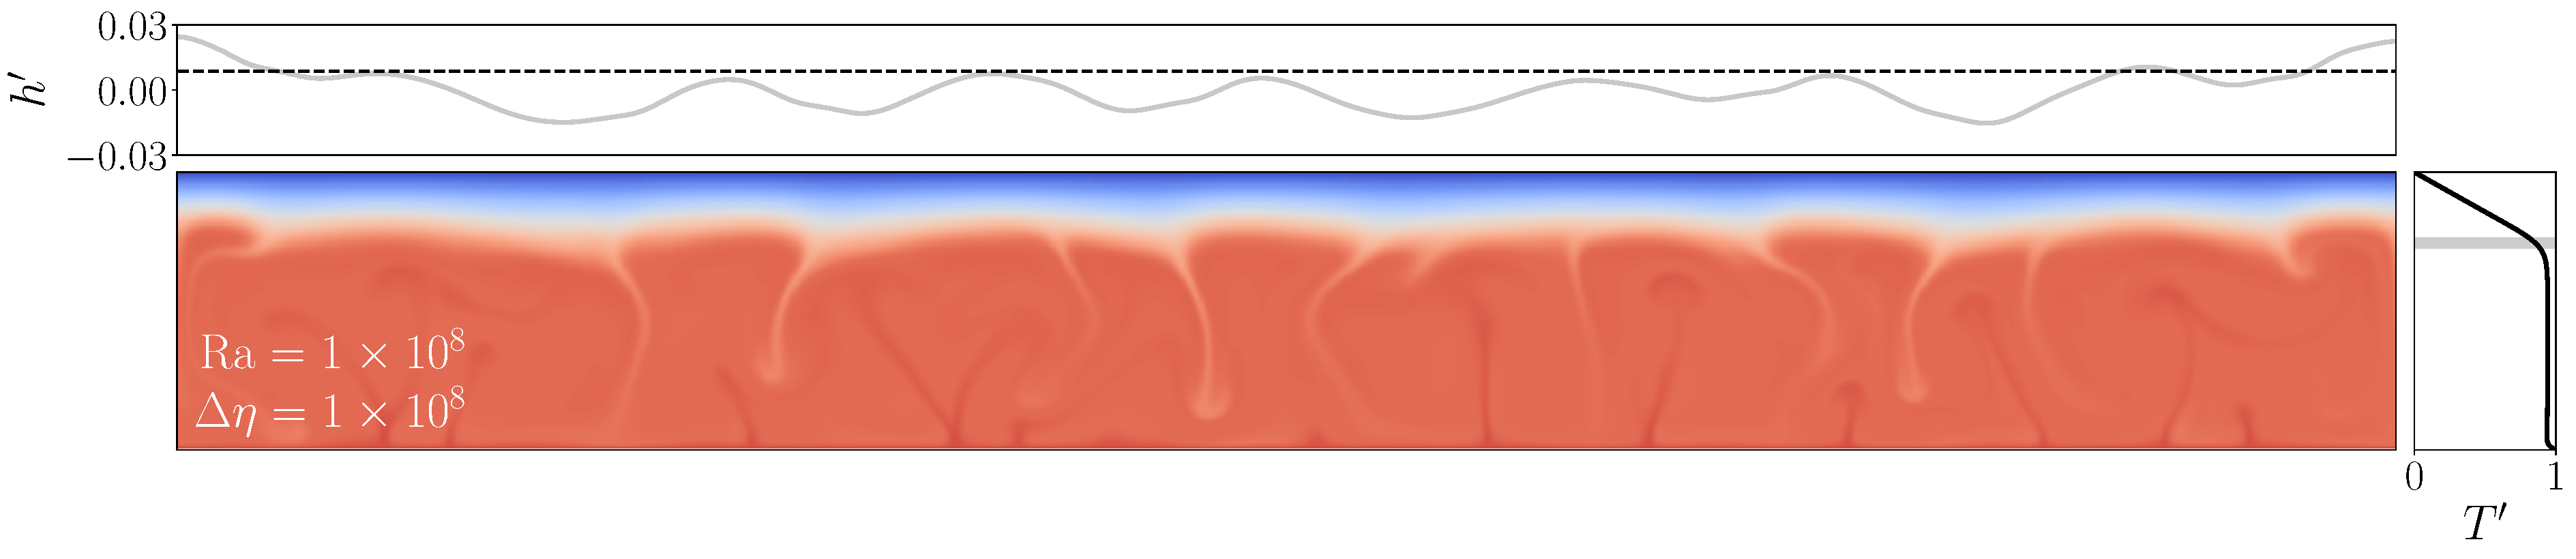
\includegraphics[width=1.0\textwidth]{T_field.pdf}
\caption[A single time snapshot of dimensionless temperatures and surface dynamic topography, for chaotically time-dependent convection in the stagnant lid regime.]{Snapshot from a single time step of the dimensionless temperature field \textit{(bottom)}, surface dynamic topography, $h^\prime$ \textit{(top)}, and temperature profile, $T^\prime$ \textit{(right)}, for chaotically time-dependent convection in the stagnant lid regime. This example shows Ra$_1 = 1 \times 10^8$ and $\Delta \eta = 1 \times 10^8$. The dimensionless temperatures range from 0 (cold; blue) to 1 (hot; red). The grey box in the temperature profile shows the instantaneous location and thickness of the upper thermal boundary layer. The vertical scale of $h^\prime$ is exaggerated.}
\label{fig:aspect-output}
\end{figure*}


The products of numerically-modelled chaotic stagnant lid convection include time-dependent, dimensionless temperature fields and surface dynamic topography profiles (Fig. \ref{fig:aspect-output}). For each case, temporally- and horizontally-averaged temperature fields are used to calculate $T_i^\prime$, Ra$_i$, and other convective parameters; full outputs can be found in Table \ref{tab:aspect-out}. Average $T^\prime$ profiles hardly vary in time, hence neither does $T_i^\prime$ nor the average position of the upper thermal boundary layer's base. Stepping up Ra$_1$ thins $\delta_{\rm rh}^\prime$, and lowers the RMS height of topography in the regime we explore numerically. Increasing $\Delta \eta$ thickens the stagnant lid because high viscosities are reached at lower depths; this is also associated with a slight increase in $\delta_{\rm rh}^\prime$. 

%The average lid base position, $y_{\rm lid}^\prime$, shifts along with chaotic instabilities---new drips and downwellings---in the upper thermal boundary layer just underneath it.





%These are shown in figure for $\Delta \eta = 10^8$, along with the time-averaged temperature profile. Characteristic to high-Ra, time-dependent convection, these temperature fields reveal diffuse upwellings and downwellings, rather than stationary plumes \todo{(ref?)}. %These different planforms alter the boundary layer stability \citep[see][]{solomatov_scaling_2000}, which would affect the scaling relationship between Ra$_1$ and topography. %As such, our assumption that rocky planets will be in the time-dependent regime of convection is a caveat of the present study.



%\todo{Q: is it useful to show histograms and mention distribution of h here? e.g. how representative is time-averaged h? Do we need to talk about ``bistability" of boundary layer thickness or is it a rabbit hole?}



\subsubsection{Fit to RMS height of topography} \label{sec:results-scaling}


\begin{table}
\centering
\caption[Topography scaling coefficients and their errors.]{Topography scaling coefficients and their errors obtained from fitting a multiple linear regression model with an interaction term to equation (\ref{eq:h_Ra_scaling}). The bottom row reports the residual variance, $\sigma^2_{\rm res}$, of the fit. \label{tab:fit}}
\footnotesize
\begin{tabular}{@{} r r r r r  @{}}
\toprule
& $A$ & $B$ & $C$ & $D$ \\
\midrule
Best fit & 9.581 & -0.5818 & -1.510 & 0.07536 \\
Standard deviation & 3.298 & 0.1859 & 0.4220 & 0.02379 \\
\bottomrule
\noalign{\vskip 1mm}
\multicolumn{5}{r}{$\sigma^2_{\rm res} = 1.584 \times 10^{-3}$} \\
\end{tabular}
\end{table}


\begin{figure}[htbp!] 
\centering    
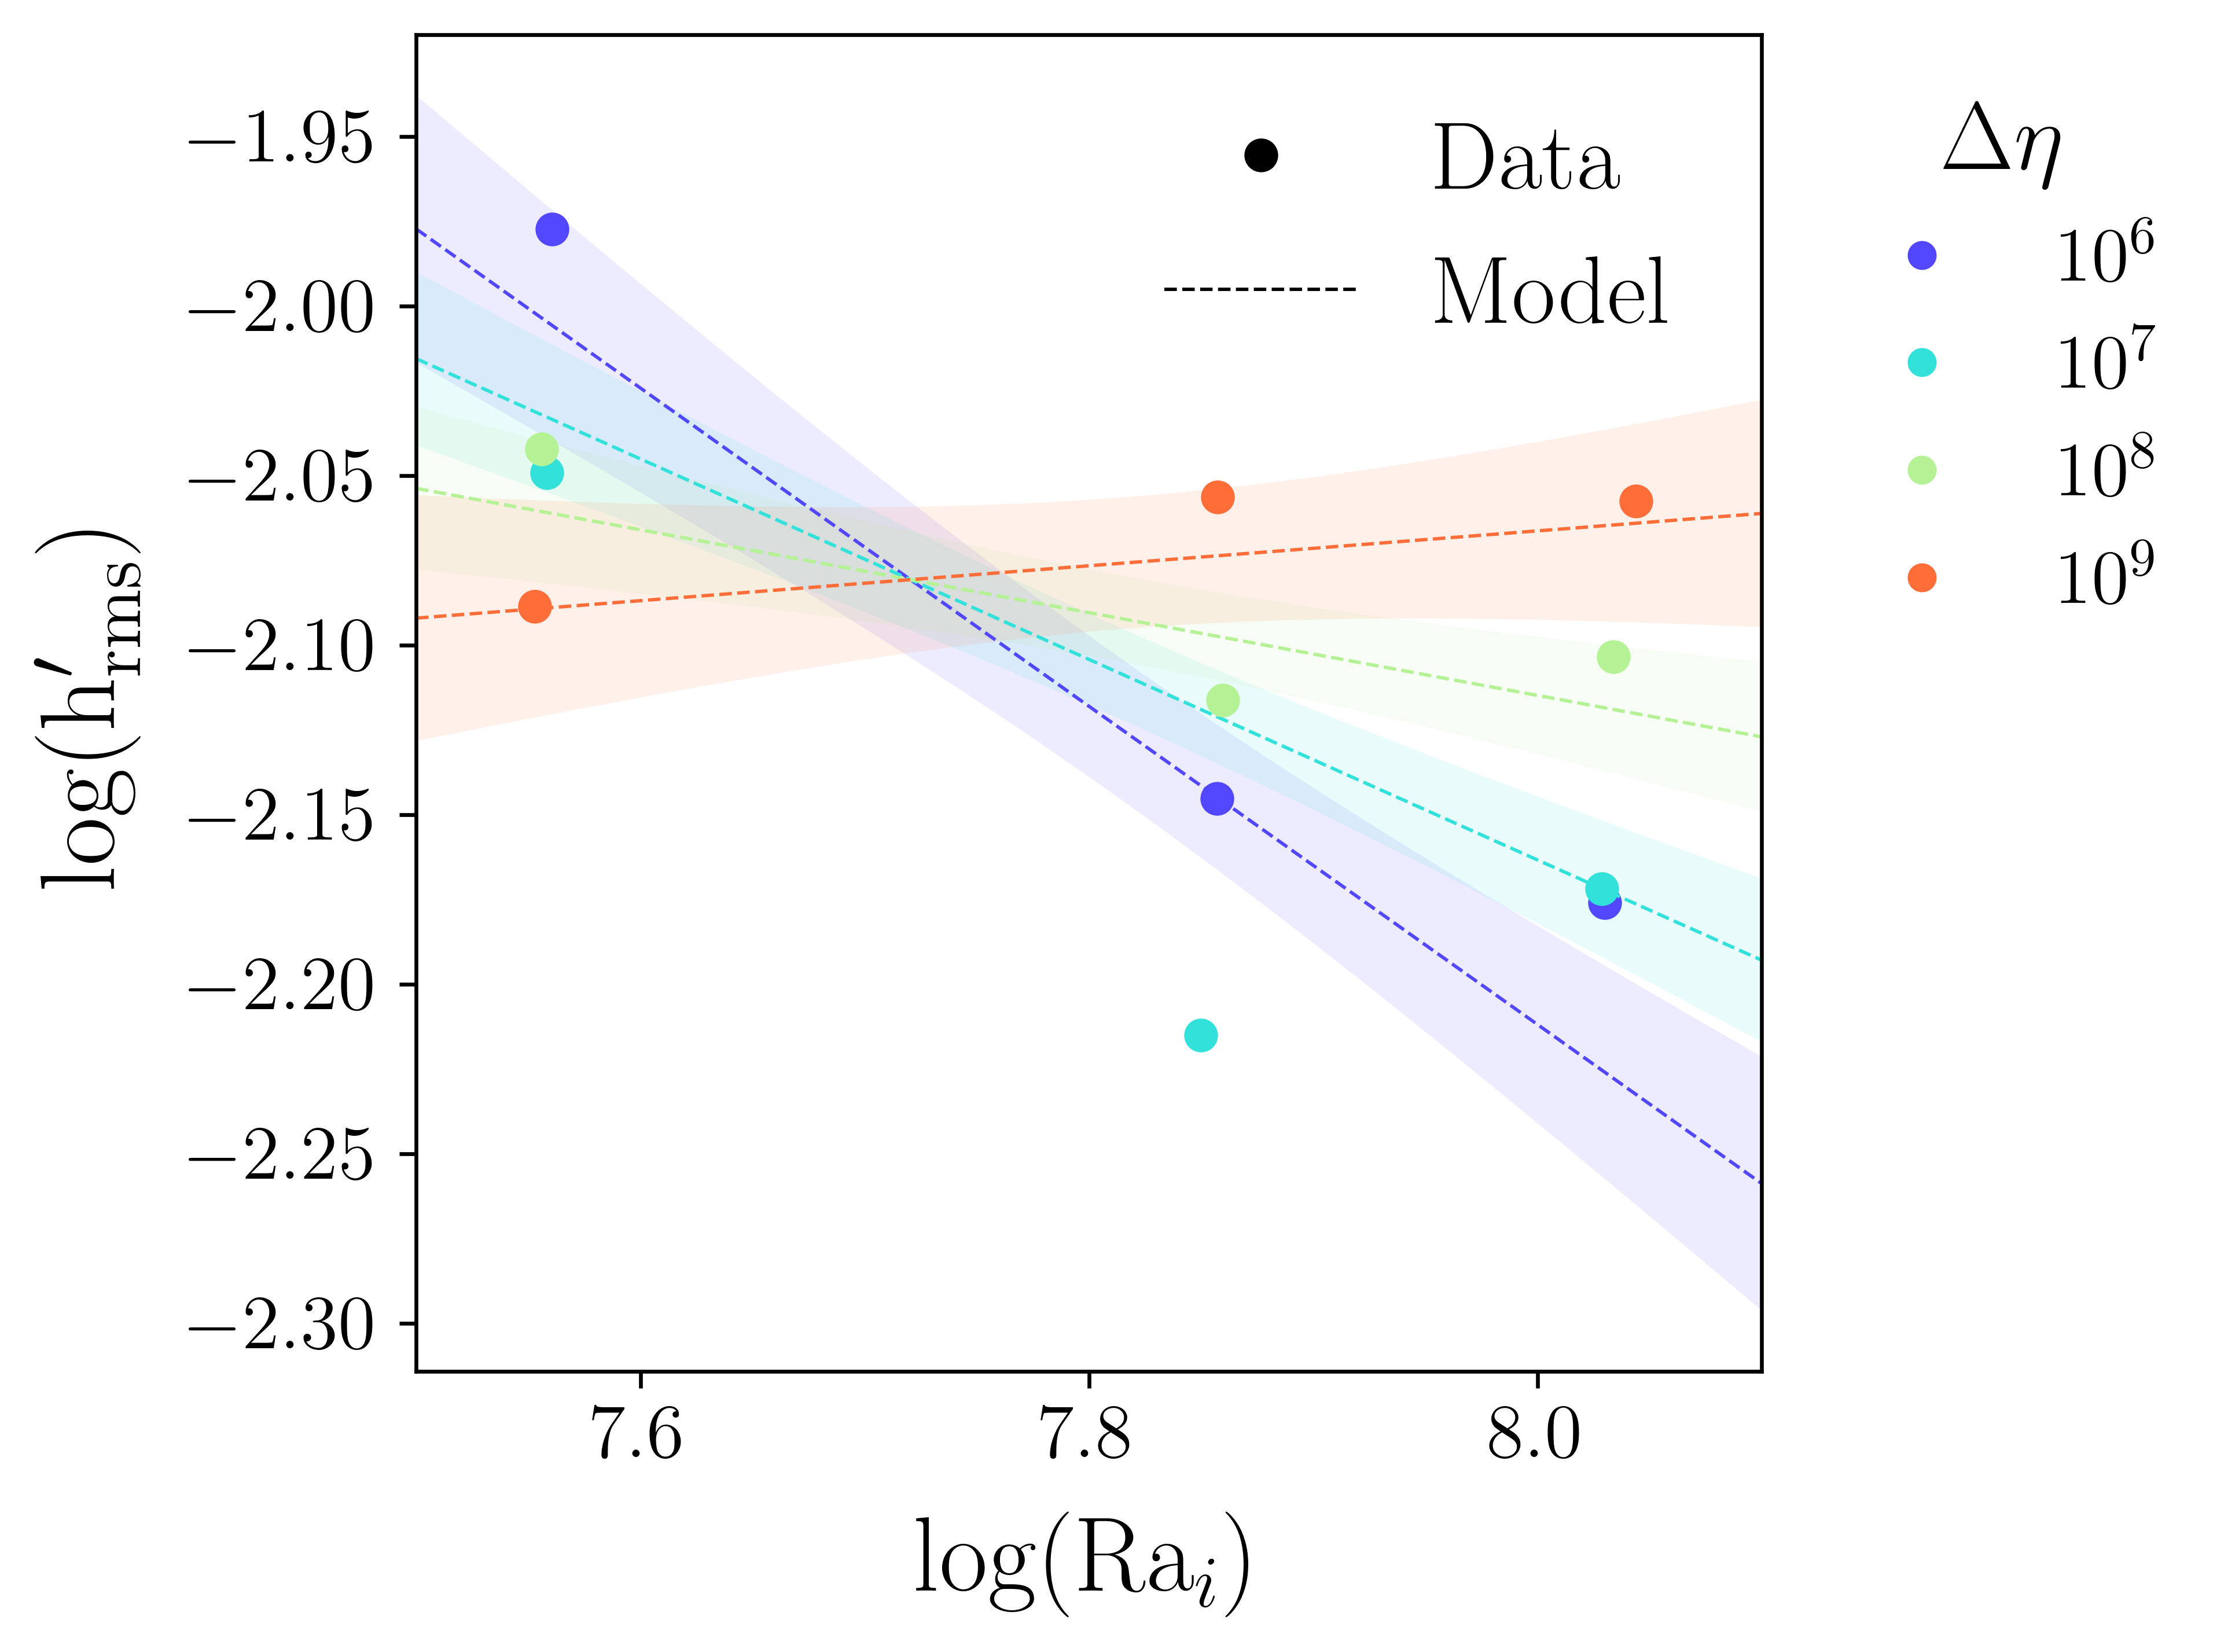
\includegraphics[width=0.6\textwidth]{h_Ra_scaling.png}
\caption[Fitted scaling relationship for dimensionless RMS dynamic topography from 2D numerical convection simulations.]{Fitted scaling relationship for dimensionless RMS dynamic topography, $h^\prime_{\rm rms}$, from 2D numerical convection simulations ($n=11$). Topography is given by a four-parameter linear model, which depends on the interior Rayleigh number, Ra$_i$, and the viscosity temperature prefactor, $b = \ln(\Delta \eta)$. Markers represent individual cases (see Table \ref{tab:aspect}) and are coloured according to $\Delta \eta$. The uncertainties on $h^\prime_{\rm rms}$, taken to be the standard errors of the mean, are smaller than the marker size. Dashed lines represent the best-fit parameter combination at discrete $\ln(\Delta \eta)$. Swaths span one standard deviation of the response variable, propagated from the covariance matrix of the fit.}
\label{fig:2D-h-scale}
\end{figure}

Fig. \ref{fig:2D-h-scale} shows the four-parameter linear fit between log($h_{\rm rms}^\prime$), log(Ra$_i$), and $\ln(\Delta \eta)$, using the functional form in (\ref{eq:h_Ra_scaling}). Best-fit parameter values and standard deviations are given in Table \ref{tab:fit}. The residual variance of this fit is $\sigma^2_{\rm res} \sim 10^{-3}$, equal to the sum of squares error divided by the degrees of freedom. Because the fitted data correspond to averages over model time, the standard errors of the mean independent and dependent variables are all small and do not impact the regression. 


The key piece of information from this section is that chaotic convection with temperature-dependent viscosity does not lend itself to constant power-law scalings of $h_{\rm rms}^\prime$ with Ra$_i$ (or Ra$_1$). The value of $\Delta \eta$ is effectively altering the slope of $\log(h_{\rm rms}^\prime)$ with $\log({\rm Ra}_i)$. Smaller viscosity contrasts of $10^7$ ($b=16$) and below are associated with strongly negative slopes. With increasing $\Delta \eta$, the slope grows systematically shallower, until it changes sign between $\Delta \eta = 10^8$ ($b=18$) and $\Delta \eta = 10^9$ ($b=20$). %(The analytic value of this point is $b=$ \todo{XX}, at which $h_{\rm rms}^\prime$ is independent of Ra$_i$.)
Conversely, the effect of Ra$_i$ on $\Delta \eta$ is such that at higher Ra$_i$ above $\sim 6 \times 10^7$, large viscosity contrasts favour high RMS topography, whilst at lower Ra$_i$ below $\sim 6 \times 10^7$, small viscosity contrasts favour high RMS topography. At Ra$_i \sim 6 \times 10^7$, these slopes ``cross over" and the effect of $\Delta \eta$ disappears. 

Evidently this behaviour is governed by a complex, chaotic system; extracting a general mechanistic understanding is compromised by the limited number of runs performed here. The effect of $\Delta \eta$ to increase $h_{\rm rms}^\prime$ may be related to thermal isostatic uplift within the stagnant lid \citep{kucinskas_isostatic_1994, moore_lithospheric_1995, orth_isostatic_2011}. We  include thermal isostasy as part of the full dynamic topography. Under a swell, hot low-density upwelling material extends to shallower depths. To compensate, the cold, dense overlying lithosphere grows thinner, and it is buoyed upwards. It can be shown that the maximum amount of thinning is directly proportional to the average lithospheric thickness. Hence, higher-viscosity-contrast convection, with its deeper lid bases, will enable a greater magnitude of thermal thinning. Meanwhile, smaller Ra$_i$ are associated with thicker $\delta_{\rm rh}$, to which dynamic topography should be proportional \citep{parsons_relationship_1983}. (For a constant $\Delta \eta$, lowering Ra$_1$ also slightly increases $D_{\rm lid}$ and thus the potential for thermal thinning.) We speculate that there is a trade-off whereby the $\Delta \eta$ effect dominates when stagnant lids are already thick and when convection is too vigorous to support high topography in its thin thermal boundary layers. Conversely, for lids that are not particularly thick, Ra$_i$ (and $\delta_{\rm rh}$) become more relevant.


A corollary of this is that at the still-higher values of Ra$_i$ expected for realistic rocky planets (up to several orders of magnitude beyond the range amenable to numerics; see discussion in section \ref{sec:discussion-extrap}), the sensitivity of $h_{\rm rms}^\prime$ to the viscosity scale becomes quite high indeed. If the absolute viscosity follows an exponential law, $\eta(T) \sim \exp(-b T)$, high $b$ is associated with low $\eta$ for the same $T$, implying low $h_{\rm rms}^\prime$. 

% \todo{---CMG: I think it would help the paper if we could explain mechanistically why we'd expect $\Delta \eta$ to control the strength of the Ra dependence. My half-baked guess is something like that raising $\Delta \eta$ leads to thicker lids, and thicker lids dampen the locally-varying thermal expansion from $\delta_{rh}$ undulations... for example:} 
% We expect high-Ra systems to have smaller amplitudes of surface topography because they have thinner thermal boundary layers. \citet{parsons_relationship_1983} showed that temperature variations near the thermal boundary layer lead to lateral variations in density caused by thermal expansion. The surface topography reflects the equilibrium height that compensates for the resulting mass distribution; that is, the surface is in thermal isostasy. Consequently, less-pronounced density variations would allow shallower fluctuations of the surface height. Independently of $\delta_{\rm rh}$, meanwhile, thicker lids might amplify the effect of lateral temperature distributions near the thermal boundary layer; the data suggest that very thick lids could even offset the weak topography over thin $\delta_{\rm rh}$. \todo{probably delete this and just say it's a complex system and hard to extract a general mechanistical explanation}




% Chaotic time-dependent convection leads to non-negligible temporal variations of $h_{\rm rms}$. These variations are not strictly measurement error (i.e., in a linear regression), but nevertheless mean that for a given Ra$_1$ and $\Delta \eta$ there is a range of expected $h_{\rm rms}$ based on numerical convection models. In fact, our runs show $h_{\rm rms}$ to be approximately bistable, but with one stable point preferred. Fluctuations in $h_{\rm rms}$ are driven ultimately by fluctuations in $T_{\rm lid}$, which affects the retrieved $\delta_{\rm rh}$ (section \ref{sec:T_retrieval}). \todo{worth it to show histograms?} 



\subsection{Parameterised modelling results}

% \subsubsection{Thermally steady-state planets}

% \todo{see Kite+ 2009 eqs 3--5}

\subsubsection{Thermal evolution}

\begin{figure}
    \centering
    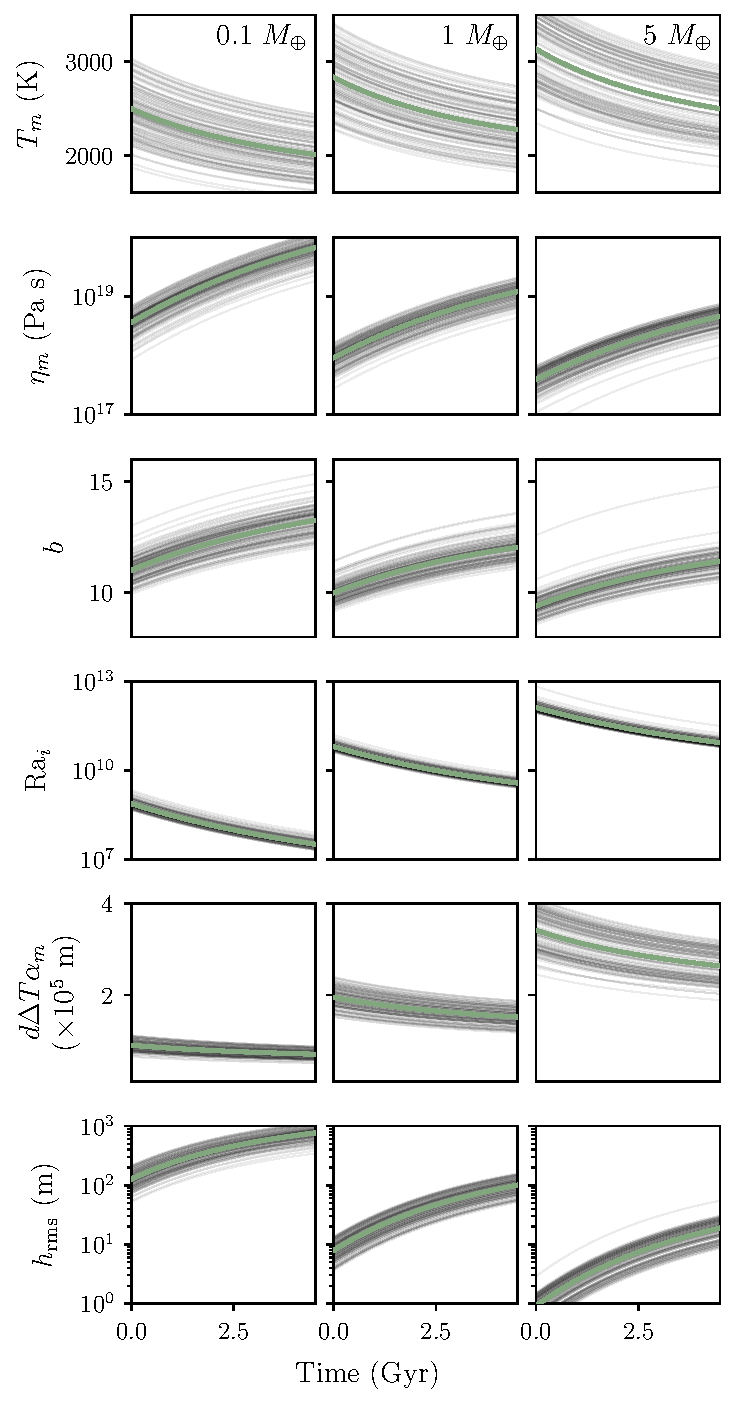
\includegraphics[width=0.6\textwidth]{evol_dist.pdf}
    \caption[Thermal evolutions sampled from the 1D model ensemble, as a function of time in Gyr.]{Thermal evolutions sampled from the 1D model ensemble, as a function of time in Gyr. From top to bottom: mantle temperature, $T_m$ in K, mantle viscosity, $\eta_m$ in Pa s, dimensionless inverse viscous temperature scale, $b$, interior Rayleigh number, Ra$_i$, topography dimensionalistion factor, $d \Delta T \alpha_m$ in m, and RMS dynamic topography, $h_{\rm rms}$ in m. Columns compare planet masses from 0.1 $M_\oplus$ \textit{(left)}, through 1 $M_\oplus$ \textit{(centre)}, to 5 $M_\oplus$ \textit{(right)}. Each thin black line ($n = 500$) represents a single evolution, drawing random values of the unknown viscosity activation energy and prefactor, hence an evolutionary spread. Green lines follow the ensemble mean (for Ra$_i$, which is log-normally distributed, this is the log-normal mean). All runs use baseline values of the core mass fraction and radioisotope budget. Parameter values and random variable distributions are given in Table \ref{tab:params}.}
    \label{fig:1D-evolution}
\end{figure}




Underlying thermal histories are sampled in Fig. \ref{fig:1D-evolution}. Because all test planets are initialised at quasi-equilibriated temperatures and stagnant lid thickness, their evolutionary paths reflect secular cooling alone, which track roughly parallel at around $-100$~K Gyr$^{-1}$. Radiogenic heating inevitably declines with age, with surface heat losses lagging behind slightly; the present-day Urey ratios are $\sim$0.65 depending on planet mass. 

Interior temperatures and Ra$_i$ increase with $M_p$ as anticipated from simple scaling laws. We expect the heat flux $q^u$ to increase linearly with planet radius for a fixed internal heat generation rate. This implies that $q^u \propto M_p^{1/3}$, ignoring compression. We can rewrite (\ref{eq:q_u})--(\ref{eq:T_rh}) as
\begin{equation}
    \eta^u = \frac{\rho_m g^u \alpha_m k_m^3 a^4_{\rm rh} \Delta T_\nu^4}{\kappa_m \left(q^u\right)^3 {\rm Ra}^u_{\rm crit}},
\end{equation}
Thus we have $\eta^u \propto M_p^{-1}$; (\ref{eq:Ra_i_1D}) leads to Ra$_i \propto M_p^2$ for approximately the same temperature difference. A five-times more massive planet has a 25-times larger Ra$_i$ \citep[see also][]{stevenson_styles_2003,  kite2009geodynamics}.

%This is close to the classical value of $\sim$0.7 \citep{schubert_whole_1980, mckenzie_parameterized_1981}.

Fig. \ref{fig:1D-evolution} illustrates how uncertainty in the viscosity law parameters $E_a$ and $\eta_0$ affects the spread and mean behaviour of the dimensional $h_{\rm rms}$ and its physical constituents over time. Temperature-dependent viscosity exhibits self-regulating behaviour: a slight increase in temperature lowers the viscosity, hence more vigorous convection via (\ref{eq:Ra}). This leads to more efficient heat loss out of the top of the convecting cell, lowering temperatures in turn. This positive feedback is not visible in a single run (which are already at quasi-steady-state in our case), but we do see the effect at play over the entire ensemble: its range of $\eta_m(t)$ is always less than an order of magnitude, despite a three-order range in $\eta_0$. Meanwhile, $T_m$ is adjusting such that $q^u$ approaches a balanced state for a given $q_{\rm rad}$ and surface area-to-volume ratio. Hence the rheological uncertainty manifests itself in $T_m$. 

We note that these calculated Ra$_i$ values are on average higher for a given $M_p$ than those commonly associated with Venus or Mars. The thermal Rayleigh numbers of real planets require some dexterity to extract, but the few constraints available suggest a value on the order of $10^6$ for Mars \citep{kiefer_melting_2003, samuel_rheology_2019}. Constraints for Venus are even more scarce, but previous work employs Ra at upper mantle temperatures on the order of $10^7$ up to $10^8$ \citep{huang_constraints_2013, king_venus_2018}. This discrepancy is partly explained by the more viscous mantles we permit in this exoplanet study. Further caveats to our Ra$_i$ estimates are discussed in section \ref{sec:discussion-Ra}.

The dimensional $h_{\rm rms}$ reflects a trade-off between $b$, Ra$_i$, and the dimensionalisation factor $d \Delta T \alpha_m$ through (\ref{eq:dimensionalise}) and (\ref{eq:h_Ra_scaling}). Extrapolating Fig. \ref{fig:2D-h-scale} would imply that, in the $b$-Ra$_i$ regime of the 1D models, high $h_{\rm rms}$ is favoured with high $b$ and low Ra$_i$. Thus deep, hot, weak mantles are doubly-inhibited from having any remarkable topography. It is clear from Fig. \ref{fig:1D-evolution} that deeper mantles are not enough to make up for lost $h_{\rm rms}^\prime$. 

Ultimately, the thermal state plays a main role in limiting the amplitude of dynamic topography. Hotter mantles necessitate lower viscosities, more vigorous convection, and thinner thermal boundary layers. Within these thinner boundary layers, there may be less scope for density variations related to thermal expansion. If we know some property of a planet to have a strong effect on its interior temperatures, then we might expect it to also impact its dynamic topography.



%Analytically, $T_m$ factors into $h_{\rm rms}$ in several places; the most relevant are that raising $T_m$ yields a greater $\Delta T$ at fixed $T_s$ and a weaker $\eta_m$. These effects compete in Ra$_i$, but the strong Arrhenius temperature-dependence means that Ra$_i$ increases with $T_m$. In $b$, again the squared term dominates and we expect $b$ to decrease with $T_m$. 



% The self-regulation of viscosity is seen in  (second row). Warmer, weaker mantles convect more vigourously, shedding heat more efficiently, cooling faster. Given several billion years of evolution, 1D models show mantles converging to a relatively narrow range of $\eta(T_{m, f}, E_a)$ regardless of the initial viscosity, $\eta(T_{m, 0}, E_a)$. Yet each $E_a$ will be associated with a different $T_{m, f}$: a natural consequence of (\ref{eq:eta-arrhenius}). That is, increasing $E_a$ will increase $T_{m, f}$ by the same amount. This raises $T_{\rm lid}$ via (\ref{eq:Tl})--(\ref{eq:T_rh})---the squared dependence on $T_m$ superseding $E_a$---thickening the stagnant lid, decreasing the effective depth of the convection cell, and lowering \Raieff. Unlike directly tweaking $d$ by changing the planet size or core fraction, none of these effects would be compensated by the dimensionalisation factor. For this reason, most of the ensemble variation in $h_{\rm rms}$ is due to variations in the viscosity law parameters. 





\subsubsection{Dynamic topography as a function of bulk exoplanetary properties}
\label{sec:results-parameters}

\begin{figure}
    \centering
    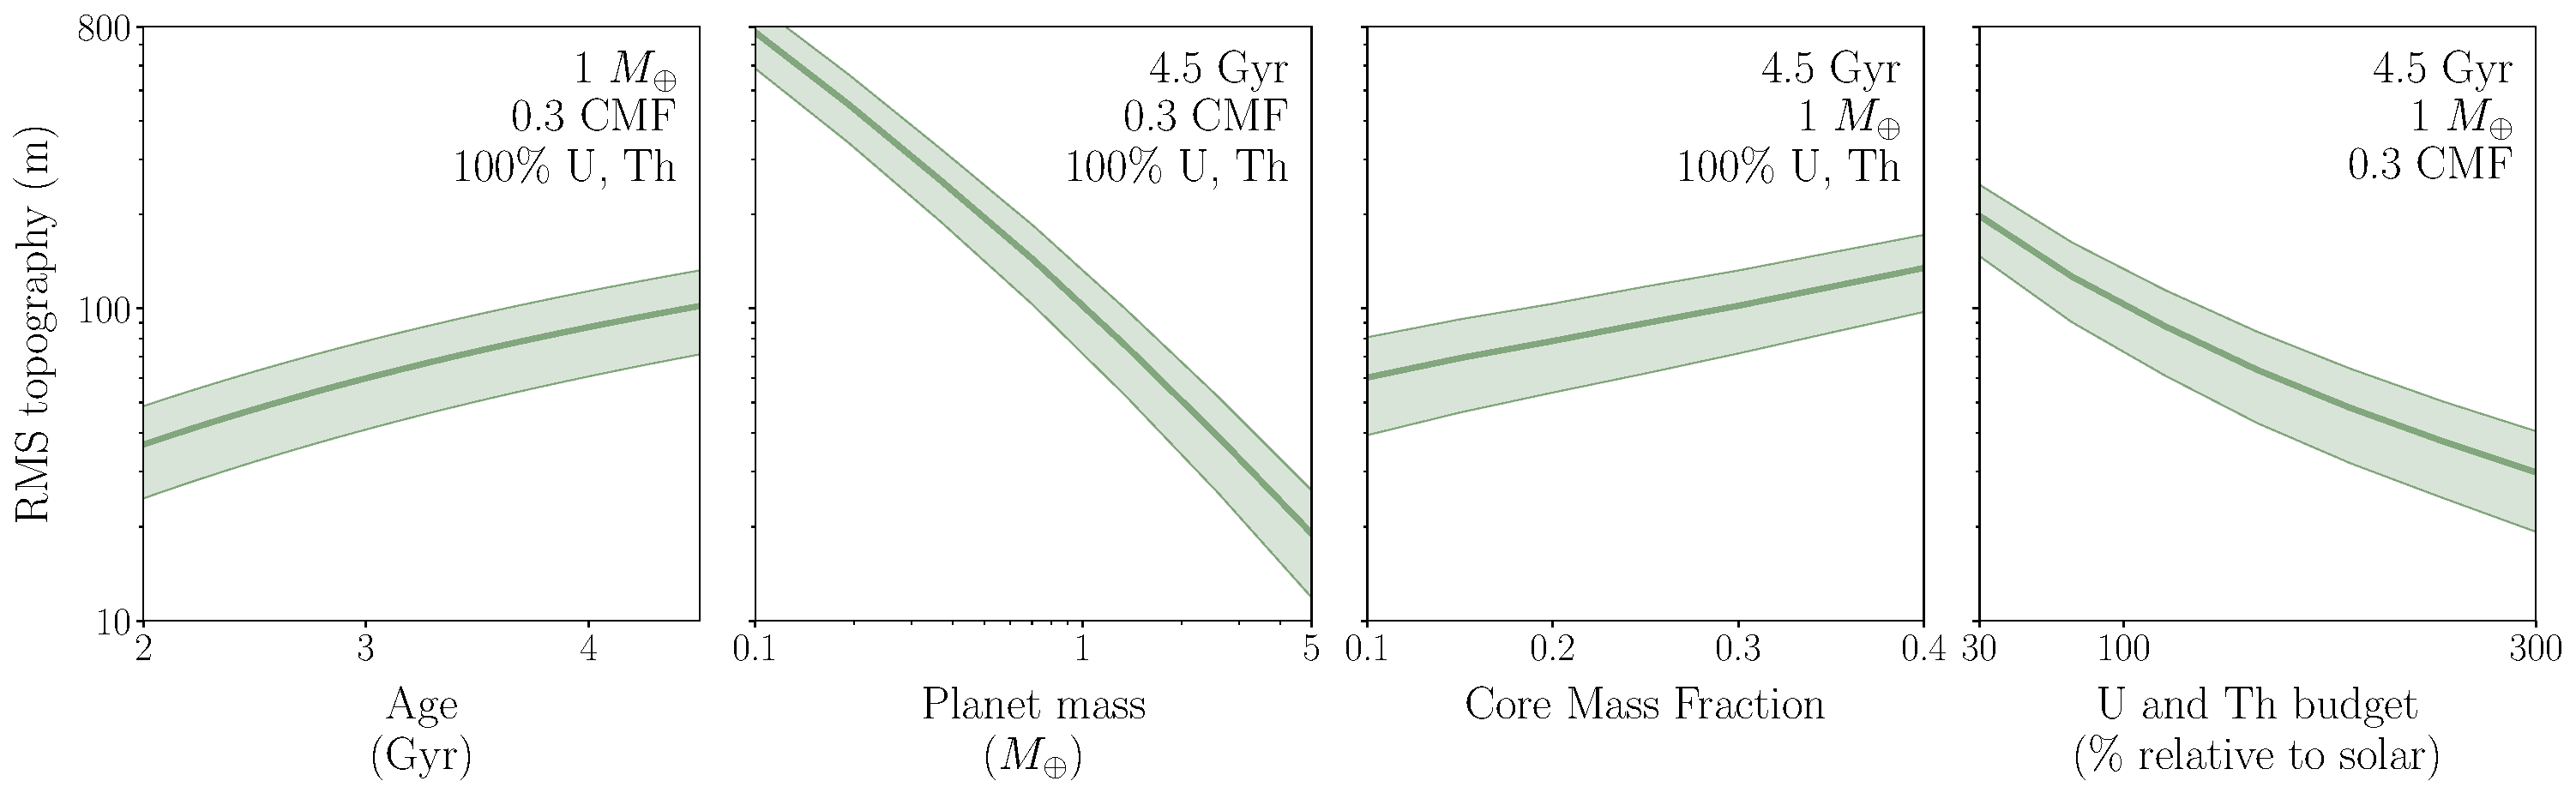
\includegraphics[width=\textwidth]{h_parameters.pdf}
    \caption[Variations of the RMS dynamic topography based on 1D thermal histories, as a function of select exoplanetary properties which might be constrained in the future.]{Variations of the RMS dynamic topography based on 1D thermal histories, as a function of select exoplanetary properties which might be constrained in the future: from left to right these are the planet age in Gyr, mass in $M_\oplus$, core mass fraction, and abundance of radioactive U and Th relative to the solar value. Solid lines show the ensemble mean of 10,000 test planets with uniformly-random viscosity activation energies and prefactors, and with normally-random topography scaling coefficients. Swaths span one standard deviation from the mean. These calculations show subaerial topography; water-loaded topography would be $\sim$1.5$\times$ higher. Parameter values and random variable distributions are given in Table \ref{tab:params}.}
    \label{fig:1D-h-scale}
\end{figure}


We now test the topographic reaction to planet age, mass, CMF, and radioisotope budget (Fig. \ref{fig:1D-h-scale}). We find $h_{\rm rms}$ to decrease with $M_p$ and $\chi_{\rm rad}$, and increase with age and CMF. Assuming that the $x$-axes in this Fig. cover the limits within which we expect to find most rocky exoplanets, then it is plausible that the resulting $y$ range marks the variability of pure dynamic topography which nature could manifest, if our scaling relationship indeed applies. The fact that $h_{\rm rms}$ drops by the largest absolute amounts over $M_p$ and $\chi_{\rm rad}$ reflects the geodynamic significance of these parameters, as well as the spread over which we would expect to find rocky planets. The senses of change of $h_{\rm rms}$ with $M_p$ and $\chi_{\rm rad}$ are predictable from their known effects on $T_m$. That is, hotter interiors are expected for massive, U- and Th-rich planets, hence lower $h_{\rm rms}$. Uncertainty in $h_{\rm rms}$ predictions is tied to uncertainty around the underlying thermal histories: yet another clue to the immeasurable usefulness of characterising this uncertainty more rigorously \citep[e.g.,][]{seales_uncertainty_2020}.

The raw values of $h_{\rm rms}$ predicted by our scaling relationship are on the order of hundreds of metres, whilst the hottest planets can exhibit mere tens of metres of dynamic topography. In fact, due to inherent self-regulation, it is difficult to achieve significantly higher topographies in our 1D model while keeping to Earth-like values of the free parameters. This result may seem very low when compared to the heights of typical topographic features seen across the Solar System. However, a fair comparison requires isolating an RMS height of just the dynamic component of topography; this is not model-independent, as we will discuss (section \ref{sec:benchmarks}). 

% \todo{[if I eventually do plug in values from Venus convection models, would mention this now...]}



\subsection{Ocean basin capacity scalings}
\label{sec:results-ocean}

\begin{figure}
    \centering
    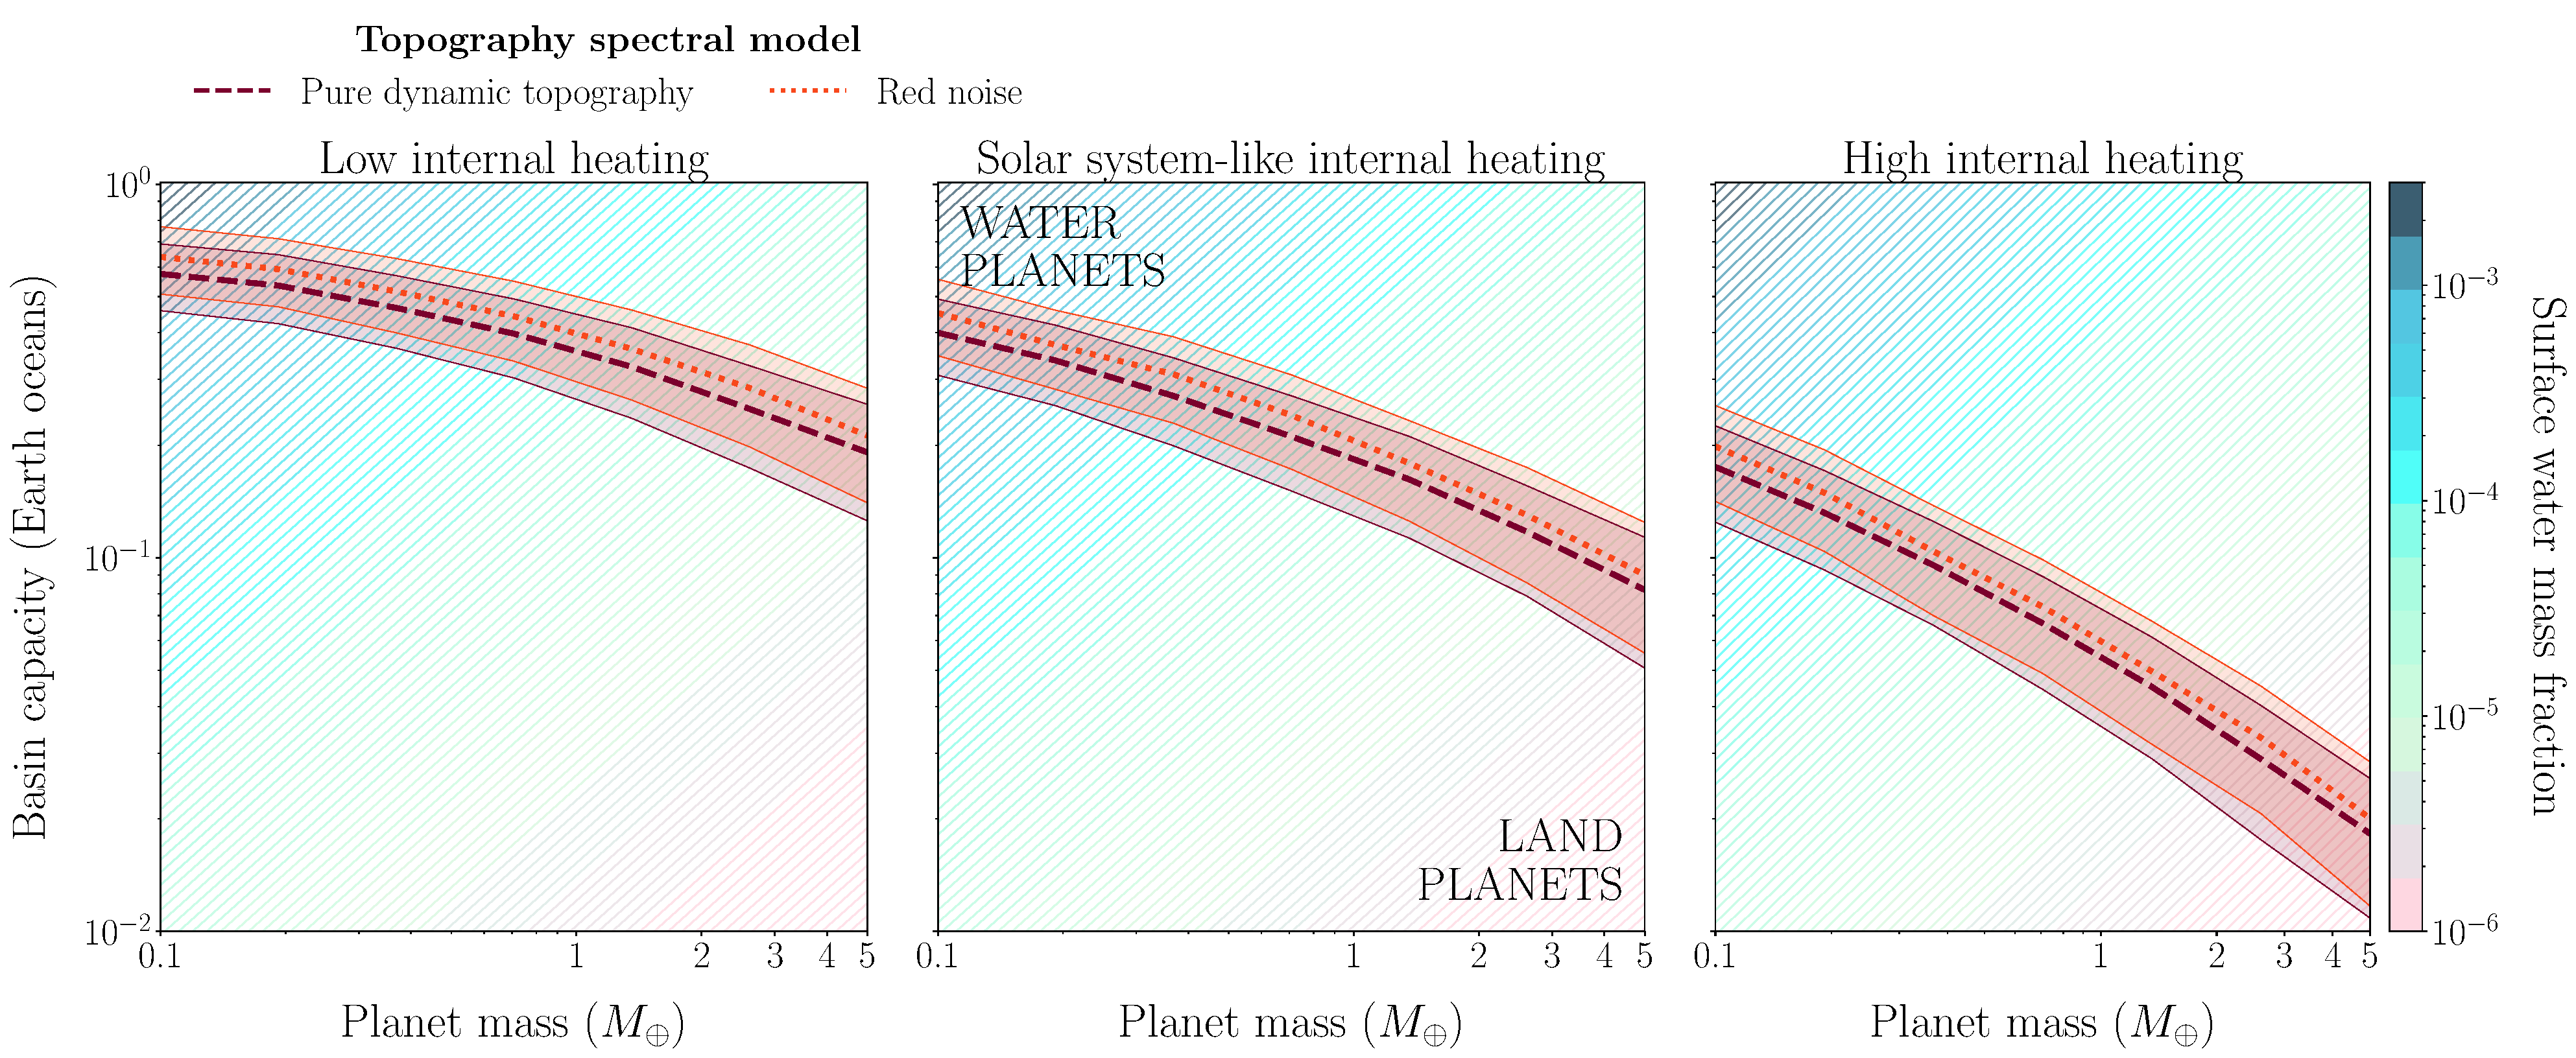
\includegraphics[width=\textwidth]{ocn_vol_ensemble.pdf}
    \caption[The competition between the ocean basin capacity and the surface water budget with increasing planet mass.]{The competition between the ocean basin capacity and the surface water budget with increasing planet mass, expressed in terms of Earth ocean volumes. The three panels are based on, from left to right, the 1st percentile value, solar value, and 99th percentile value of expected mantle heat production across rocky exoplanets \citep{nimmo_radiogenic_2020}. Basin capacities as a function of planet mass are calculated from either the pure dynamic topography spectral model (dashed purple lines) or the red noise model (dotted red lines). The empirical Venus model overlaps the pure dynamic topography and is not shown. Random rheological parameters propagate through the model; the resulting 1$\sigma$ variation is represented by the swaths. In the background, the solid contours follow lines of constant surface water as a fraction of planet mass (note a modern Earth value of $\sim$200 ppm). Thermal histories refer to a 4.5-Gyr planet with a core mass fraction of 0.33.}
    \label{fig:ocn-vol}
\end{figure}

We have tested three fiducial spectral models to find a relationship between the RMS and peak value of dynamic topography. The theoretical red noise model, the empirical Venus model, and the numerical dynamic topography model all produce an $h_{\rm peak}$ which is, on average, some constant scalar multiple of $h_{\rm rms}$. For both numerical dynamic topography and the total Venus topography, $h_{\rm peak} \approx 3.5 h_{\rm rms}$, and for red noise topography, $h_{\rm peak} \approx 3.9 h_{\rm rms}$. (For a pink noise structure similar to Earth's observed dynamic topography, $h_{\rm peak} \approx 4.0 h_{\rm rms}$.) 

We use our $h_{\rm peak}$ estimations to derive the ocean basin volume capacity $V_{\rm cap}$ as a function of planet mass (Fig. \ref{fig:ocn-vol}). This quantity represents the smallest volume of surface liquid water that would entirely inundate a planet. The actual land fraction requires knowing the ocean mass. We leave sea level as an unknown quantity and simply consider fiducial surface water budget scenarios. Specifically, we treat the amount of surface water as a constant mass fraction of $M_p$. This parameterisation brackets the planet's total water budget with its volatile partitioning between the interior and exterior---in reality the amount of water stored in the mantle would affect the planet's thermal evolution through its rheology (and melting history, which is not modelled). 

As the basin volume capacity changes with $M_p$, so too does the water volume corresponding to this mass fraction (we assume a density of $1000\,\rm{kg\,m^{-3}}$; salt water is slightly denser). Fig. \ref{fig:ocn-vol} can be read as follows: for a given surface water budget, the planet mass where this contour intersects the basin capacity gives the most massive planet that could sustain land with dynamic topography alone. For example, a 1-$M_\oplus$, 4.5-Gyr-old planet endowed with solar U and Th could hold about 0.3 Earth oceans on its surface. The internal heating rate has a strong influence on $V_{\rm cap}$.


Fig. \ref{fig:ocn-vol} compares different assumptions about the spectral distribution of topography, which would affect the relationship between the peak and RMS topography. The dynamic topography and Venus models overlap identically, and the red noise spectrum results in only slightly larger $V_{\rm cap}$, seemingly because they are very similar in the low-degree regions where most of their power is concentrated. The basin volume corresponding to an infinitesimally-small but nonzero land area is insensitive to the distribution of topography at high frequencies.






% \jr{I think some simple equations and some back of the envelope numbers would help the reader here. If I understand correctly, the basin capacity is just $M_\text{cap} = 4 \pi R_p^2 \rho_w h_{\text{peak}}$. For Earth's ocean mass ($1.4 \times 10^{21}$~kg) that means a peak topography less than 2.7 km leads to a waterworld. If $h_{\text{peak}}$ didn't vary with planet mass, we'd expect $M_\text{cap} \propto M_p^{2/3}$ because of the surface area term. We have $h_{\text{peak}}$ slightly decreasing with increasing mass, so we don't see quite as steep a slope as $\propto M_p^{2/3}$ on Figure 7, but that does explain the main trend.}





We can formulate these results in terms of a simple scaling analysis. Equation (\ref{eq:ocean-integral}) can be written as $M_\text{cap} = 4 \pi R_p^2 \rho_w  \rho_m / (\rho_m - \rho_w) h_{\text{peak}}$, where $M_\text{cap}$ is the ocean basin capacity in kg. For Earth's ocean mass ($1.4 \times 10^{21}$~kg), this means a peak topography $h_{\text{peak}}$ less than 2.7 km leads to a waterworld. If $h_{\text{peak}}$ were independent of planet mass, we would expect $M_\text{cap} \propto M_p^{2/3}$ due to the increase in surface area alone (the mass-radius relation in (\ref{eq:MR}) gives a slightly shallower power due to compression). However, we have $h_{\text{peak}}$ strongly decreasing with increasing mass. For dry olivine and solar U and Th abundances, $h_{\text{peak}} \propto h_{\text{rms}} \propto M_p^{-0.5}$. From (\ref{eq:ocean-integral}), $M_\text{cap} \propto R_p^2 h_{\rm peak}$, so $M_\text{cap} \propto M_p^{0.04}$ using (\ref{eq:MR}). Warmer, less viscous interiors decrease this exponent, so the most massive rocky planets have the smallest basin capacities even though they have the largest surface areas. If the pressure of a topographic load is balanced only by a constant compressive strength of the crust rock, we have $h_{\rm peak} \propto g^{-1}$, and the resulting proportionality $M_{\rm cap} \propto M_p^{0.08}$ is also quite flat (though the overall basin capacity would be higher). We are being conservative about how likely planets are to have dry land by considering only dynamic topography.

It is important to emphasise that the basin capacities shown in Fig. \ref{fig:ocn-vol}, based on dynamic topography alone, are likely underestimating the true value. The observed topographies of Venus, Earth, and Mars produce basin capacities of 3.4, 3.3, and 2.9 Earth oceans respectively, whereas the model produces basin capacities of \textless1 Earth ocean. The peak and RMS elevations of our terrestrial planets are much higher than those predicted by the dynamic topography scaling here. Other mechanisms contribute to supporting higher topography on planets. Also, our model may under-predict dynamic topography for a given planet mass, as we will discuss in the next section.






%%%%%%%%%%%%%%%%%%%%%%%%
\section{Discussion}
\label{sec:discussion-top}

\subsection{Expanding RMS topography} \label{sec:discussion-spectrum}

Fig. \ref{fig:ocn-vol} suggests that reasonable changes to the spectral distribution of topography have no strong effect on how peak dynamic topography scales with planet mass, and hence on the volume of water that could be contained below this highest point. Our concern with topography's characteristic harmonic structures might thus seem somewhat tangential to (or in the worst case, distracting from) the basic problem that this study purports to address. However, these details would become more of a concern if the field can mature---and especially if we hope, someday, to use informed topography distributions as a boundary condition in exoplanet climate models \citep[e.g.,][]{turbet_habitability_2016, rushby_effect_2019}. For example, the volume calculated in (\ref{eq:ocean-integral}) represents the amount of water that would flood a planet exactly, leaving just an island with infinitesimally-small area. Yet in principle one could also calculate the maximum basin size associated with any arbitrary land fraction. These intermediate land fractions may be much more sensitive to spectral complexities, such as wide plains or anisotropic mountain ranges.


The initial questions here have justified simplified harmonic structures of topography as such. Specifically, we have presumed a log-linear model of the power spectral density, which is to say that the variance of elevation is a power-law function of the horizontal distance scale. Although this relationship is probably suitable at low orders \citep{turcotte_fractal_1987}, contemporary workers now know the behaviour to be much more nuanced. Local estimates of topography's spectral slope can appear notably inconstant---i.e., the surface roughness is heterogeneous---but these differences are captured by further power laws of other statistical moments (i.e., a ``multifractal''), out to virtually-infinite order, all culminating neatly in a mathematical model with three scale-invariant parameters \citep[e.g.,][]{pelletier_selforganization_1999, gagnon_multifractal_2006, lovejoy_scaling_2007, alisaberi_percolation_2013, liucci_fractal_2017, rak_universal_2018, landais_multifractal_2019, keylock_holderconditioned_2020}. One of these parameters relates to the spectral slope; the other two relate to spatial heterogeneity. \citet{landais_topography_2019} have demonstrated the use of such a descriptive model for synthesising surface relief of arbitrary rocky planets. Thus, the framework does exist for representing randomised global topography layouts to a high degree of statistical realism using a simple model. 

The hitch is that these multifractal parameters are currently determined on a case-by-case basis. That is, the surfaces of real planets must be mapped to high spatial resolution, and then reduced to a multifractal representation. This is because multifractal models of topography \citep[e.g.,][]{landais_topography_2019} are still only descriptive; they do not explain the physical connection between the input parameters and planet bulk properties such as mass. (The exception is the parameter related to spectral slope, which is similar on Earth and Mars and may be a signature of dynamic topography.) Thus multifractals' gain in descriptive accuracy may not translate to predictive power for distant exoplanets. After all, there are very few geomorphologically-active bodies in the universe with mappable topography, from which we could tie observed pattern(s) to geophysical process(es).


Nevertheless, it is worth mentioning that a predictive numerical model of topographic power spectra has been developed for at least one other specific terrain-building endmember process---impact cratering---which would pertain to short wavelengths \citep{rosenburg_topographic_2015}. This model complements our study's contribution of the endmember process of dynamic topography. Towards these smaller scales, quantitative models of landscape evolution \citep[e.g.,][]{perron_controls_2008, lipp_scaledependent_2021} may eventually prove useful for building even a very preliminary understanding of the slope distributions of exoplanets. Topography at the landscape scale, via its first-order control on erosion rates, may prove highly relevant for planet-scale processes such as a silicate weathering climate feedback \citep{graham_thermodynamic_2020}.






\subsection{The role of rheology and its uncertainties} \label{sec:discussion-rheology}


Any deterministic prediction of $h_{\rm rms}$ will be hindered by the unknown mantle rheology. Increasing the activation energy of viscosity from 240~$\rm{kJ\,mol^{-1}}$ to 300~$\rm{kJ\,mol^{-1}}$ will double $h_{\rm rms}$ for an Earth-mass planet, all else being equal. This uncertainty propagation is built into our model via the scaling functional form in (\ref{eq:h_Ra_scaling}). $E_a$ enters this equation twice, in both $b$ and Ra$_i$ (via $\eta_m$). Particularly in the high-Ra$_i$ regime, small changes in the viscosity contrast parameter $b$ create large changes in $h_{\rm rms}^\prime$ (Fig. \ref{fig:2D-h-scale}). 

We have attempted to capture some of the rheological uncertainty by varying $E_a$ and $\eta_0$, the free parameters in the Arrhenius viscosity law (\ref{eq:eta-arrhenius}). However, we cannot claim that our results are propagating nature's true variability. Firstly, the underlying covariance of these parameters is not known. The prior range employed by our study covers only pure olivine and pure orthopyroxene, and roughly so at that. \citet{spaargaren_influence_2020} also parameterise the mineralogical control on viscosity with an extra prefactor that increases over three orders of magnitude, calibrated between ferropericlase-rich (high Mg/Si) and stishovite-rich (low Mg/Si) lower mantle compositions \citep{xu_silicon_2017, ballmer_persistence_2017}. Relating the rheological parameters to the lower or upper mantle composition in a realistic way requires not only a complex thermodynamic model predicting these mineral compositions, but also a dataset of strain rates from experiments and \textit{ab initio} mineral physics. The actual strain rate of an olivine-orthopyroxene aggregate is certainly not a simple combination of diffusion creep flow laws. Further, in practice, real mantle viscosities will be strongly sensitive to their water content, unlikely to ever be known for a given exoplanet.

The second reason why we are not capturing the true variation is that our fixed rheological model ignores structural uncertainty by design. We have only considered diffusion creep with no pressure dependence, but the creep mechanism depends on shear stress and is not known \textit{a priori}. Including pressure dependence in the parameterisation (with adiabatic profiles from an interior structure model, for example) would lead to higher viscosities and sluggish flow in the lower mantle. Importantly, and in particular for more massive planets, this fact could render the viscosity self-regulation less efficient \citep{stamenkovic_influence_2012}, meaning that internal temperatures for evolved planets become much more sensitive to initial temperature conditions, and the resulting $h_{\rm rms}$ scatters more widely (overall, retaining a hotter mantle at older ages will reduce $h_{\rm rms}$). Uncertainty would grow severer still if one allowed for complex rheological features such as a low-viscosity asthenosphere \citep{bodur_impact_2019}, which manifests in smaller-scale dynamic topography on Earth \citep{hoggard_global_2016}. Finally, technically, the lithosphere itself obeys a distinct viscoelastic rheology, and coupling these dynamics to a convection model would also modify its topography amplitudes \citep{patocka_stress_2017}---we have ignored elastic effects in this attempt (section \ref{sec:elastic}).

All this rheological uncertainty is worth discussing because dynamic topography is apparently sensitive to both viscosity's absolute value and how it changes over the boundary layers \citep{hager_longwavelength_1989}. Low viscosities imply higher temperatures and low convective stresses. For the isoviscous case, the association of low viscosity with low topography can be seen clearly in Table 2 of \citet{lees_gravity_2020}, from which we get a numerical scaling of $h_{\rm rms}^\prime \propto \eta^{-0.6}$, with interior temperature and lithospheric thickness fixed. If we have two isoviscous layers with a stiffer top layer (i.e., approximating a cool viscous lithosphere), then there is an analytical solution for the surface normal stress induced by a spherical density anomaly at some depth \citep[equation (34) in][]{morgan_gravity_1965}. In this solution, the effect of relative viscosity is strongest when density anomalies are nearer the surface.






\subsection{Caveats to topography predictions from numerical convection}  \label{sec:discussion-modelling}

In determining a scaling relationship for the RMS and peak amplitudes of dynamic topography from numerical convection, we have assumed that details of our methodology can produce generalisable results. This section discusses some important caveats.

\subsubsection{Low-order power} 
\label{sec:discussion-loworder}
%Our model topography spectra would only be informative for a certain range in dimensionless wavenumber, subject to the numerical modelling setup. 
The contribution to the total power drops off quickly with spherical harmonic degree for the spectral slopes used here. Consequently, the overall RMS amplitude is unaffected by the high-frequency power, whilst the low-frequency power has a disproportionately large influence. Our simulations show a flattening-out of the topography power spectra as we go to wavelengths larger than twice the layer depth. Yet topography on Venus clearly exhibits long-wavelength features (Fig. \ref{fig:top-spectra}). On Earth, the dynamic topography power is largely concentrated at degree 2 \citep{hoggard_global_2016, 2021GeoJI.225.1637Y}. The relatively simple rheologies in our model cannot produce these features. Long-wavelength mantle flow on Earth may be deeply entwined with the presence of an asthenosphere and tectonic plates, themselves entwined further \citep{lenardic_boot_2019}.

Mars provides a case that's different still. Its topography is dominated by a degree-1 signal; that is, Mars shows an asymmetry where the southern hemisphere sits higher than the northern, and the volcanically-constructed Tharsis plateau dominates the east side of the former. Whilst this pattern is thought to be related to degree-1 mantle convection, as of yet there is no fully-endogenous mechanism consistent with all the observables \citep{roberts_chapter_2021}. Regardless, the processes we model will never lead to such a convection pattern. The possibility of degree-1 convection could further complicate our preliminary scaling relationship between $h_{\rm rms}$ and Ra.



\subsubsection{Geometry and heating mode effects}

Our numerical convection simulations were performed exclusively in a bottom-heated 2D box. For 2D isoviscous models, RMS topography appears consistent across Cartesian and cylindrical geometry, with a scaling exponent on Ra close to $-$1/3 as expected from theory \citep{mckenzie_convection_1974, parsons_relationship_1983}. However, in the non-isoviscous settings we study here, this scaling is not necessarily insensitive to the model geometry. It remains to be seen how higher spatial dimensions, or cylindrical or spherical geometry, would explicitly affect $h_{\rm rms}$. Internally-heated convection---best described with an altogether different formulation of the Rayleigh number---tends to result in different convective planforms and may also show different patterns with respect to dynamic topography \citep[e.g.,][]{orth_isostatic_2011}. This distinction between heating modes would be especially relevant for young planets with high radioisotope concentrations.




% \todo{[TODO: are there no direct comparisons to be found in the literature of boundary layer thicknesses between geometries/heating modes in chaotic, non-isoviscous models..? haven't been able to find]}

\subsubsection{Filtering in the lithosphere} \label{sec:elastic}

In reality, the peak amplitude of dynamic topography is modulated by the flexure of the elastic lithosphere, which depends on the lithosphere's effective elastic thickness. Thin elastic lithospheres (expected for hot stagnant lid planets such as Venus) could bring a $\lesssim 5\%$ reduction in dynamic topography \citep{golle_topography_2012, dumoulin_predicting_2013, patocka_elasticity_2019}. Here we omit this filtering for simplicity and instead predict an upper limit of dynamic topography.

In addition to these elastic effects, %the thickness and density of the crust could change dynamic topography amplitudes \citep{sembroni_impact_2017}. 
the lithosphere can deform plastically in response to convective stress, as illustrated by the crustal thickening example in Fig. \ref{fig:topography-schematic}b \citep{kiefer_mantle_1991,pysklywec_timedependent_2003, zampa_evidence_2018}. We have not considered higher-order effects from the formation of a crust, whose marginally lower density with respect to mantle rock would buoy topography slightly higher.


% A realistic elastic lithosphere acts as a low-pass filter on instantaneous dynamic topography. Indeed, accounting for these elastic effects carefully has received dedicated effort \citep{golle_topography_2012, dumoulin_predicting_2013, patocka_elasticity_2019}, showing that thin elastic lithospheres (expected for hot stagnant lid planets such as Venus) are associated with a \textless 5\% reduction in dynamic topography.

% \todo{... probably not worth it but maybe to show some rough plots e.g. using fourier filters from Lees+ Appendix A? requires a bunch of parameters... }

% \subsubsection{Erosion}

% On real planets, the instantaneous topography is a balance between uplift and erosion. While rates of uplift could be inferred from the convective timescale\todo{[unsure exactly if this is true?)]}, this model has perhaps glaringly left out erosion, the rate of which would depend strongly on the main agent (e.g., solid or liquid water, wind/dust) and the climate. Whilst erosion would indeed decrease the amplitude of dynamic topography overall, spectral analyses of river profiles on Earth by \citet{roberts_generation_2019} have shown that (i) large-scale processes (i.e., geodynamic uplift) might be said to shape fluvially-eroded landscapes to a first-order approximation because most of the spectral power is at low harmonic degrees; and (ii) fluvial erosion appears to be scale-invariant at wavelengths longer than 10~km, with a similar spectral slope to that inferred for dynamic topography. Hence we might ignorantly postulate that erosion by running water would not hinder our assumption of a universal spectral slope. \todo{although it would affect the amplitude no?? not sure about ice, which seems like it would smooth things out at a larger scale... and of course post-glacial rebound is a fact of isostasy and by definition doesn't affect dynamic topography. amplitude decrease due to erosion would compete with amplitude increase from including extrusive melting/crustal thickening/isostasy

% \todo{also cite \citet{pelletier_self-organization_1999} here}


\subsubsection{Paucity of ground truths}\label{sec:benchmarks}

Ultimately, making accurate predictions of dynamic topography amplitudes is meaningless without accurately measuring them somewhere. It is not trivial to isolate the dynamically-supported component of the cumulative topography we observe. Serious efforts at separating out the isostatic component on Venus rely on knowing the associated admittances, simulated or inferred from a crustal thickness estimate \citep{mckenzie_relationship_1994, pauer_modeling_2006, wei_gravity_2014, yang_separation_2016}, to leave a result that is not model-independent. 

For Earth, meanwhile, estimates of oceanic bathymetry less its age-depth cooling pattern can been used to navigate this impasse, revealing dynamic topography peak amplitudes of $\sim$1~km \citep{hoggard_global_2016, hoggard_oceanic_2017}. Although this result happens to align with our Earth-mass planet predictions, a direct comparison demands caution because we have been modelling stagnant lid planets---modern Earth is evidently outside this regime. Sections \ref{sec:discussion-rheology} and \ref{sec:discussion-loworder} have mentioned how the pattern of Earth's dynamic topography is a consequence of its experiencing convection under plates. Any plate behaviour is not captured in our numeric simulations. Indeed, dynamic topography observed on the only known planet with plate tectonics seems to reflect both deeper mantle flow and shallower lithospheric and aesthenospheric structure, as well as the coupling between them \citep{davies_earth_2019}. Nor is our 1D thermal history model strictly applicable: the thick, insulating lids imposed by the stagnant lid regime would lead to underestimated surface heat flow for a plate tectonics regime. Note further that this $h_{\rm peak}\sim1$~km estimate for Earth purposefully excludes the thermal bathymetry of mid-ocean ridges, a plate-scale topographic expression which could technically could fall under dynamic support.



\subsection{Caveats to using scaling relationships}


\subsubsection{Sensitivity to functional form}

A scaling law will never be more than a mathematical shortcut: a tool to preempt heavy model running for any imaginable parameter combination. This work has adopted a log-linear scaling for dynamic topography in terms of the Rayleigh number and rheological temperature scale of convection. Whilst this choice of independent parameters is indeed physically justified, it is not unique in being justifiable. %Nevertheless, Ra numbers are convenient because they are dimensionless. Thus the slope of a log-linear fit is not subject to dimensional constraints---compared, for example, to an alternative dimensional heuristic, $h_{\rm rms} \propto \alpha \Delta T_{\rm rh} \delta_{\rm rh}$, which precludes slopes other than unity. Yet 
We emphasise that the result of this study---that dynamic topography becomes essentially negligible with hotter (younger, deeper more radioactive) mantles---is fundamentally a consequence of our scaling functional form.

The interaction between $\Delta \eta$ and Ra$_i$ in our scaling somewhat complicates a comparison with previous power-law relationships for isoviscous convection---recall that constant-viscosity convection is described by a single value of the Rayleigh number. Boundary layer theory suggests that $h^\prime \sim {\rm Ra}^\gamma$ \citep{mckenzie_convection_1974, parsons_relationship_1983} with $\gamma=-1/3$, whilst more recent 3D Cartesian simulations of \citet{lees_gravity_2020} have $\gamma$ ranging from -0.289 to -0.342. Under our scaling function, an equivalent exponent to $\sim -1/3$ on Ra$_i$ is met at high values of $b \sim -23.7$, at which $h_{\rm rms}^\prime$ could be said to scale similarly to the isoviscous case. 
% b = (-1/3 - C) / D


\subsubsection{Extrapolation across Rayleigh numbers} \label{sec:discussion-extrap}

For Ra$_1$ much greater than $3 \times 10^8$, the highest value considered in our experiments, one may be waiting prohibitively long for numerical convection models to converge. Yet the thermal histories we have produced in 1D tend to deliver these very large, out-of-range Rayleigh numbers (Fig. \ref{fig:1D-evolution}). Wielding the numerical scaling to estimate $h_{\rm rms}$ thus necessitates an extrapolation over up to four orders of magnitude in Ra$_i$. (Meanwhile, values of the 1D $b$ analogues are indeed accessed in 2D.) This projection into high-Ra$_i$-space has unproven fidelity, and brings a heavy caveat to our results. Namely, extrapolating scaling functions for convection rely on there being no regime change or otherwise discontinuous effects in the region to which we are blind. Yet the fitted function (Fig. \ref{fig:2D-h-scale}) indicates complex interactions between Ra$_i$, $b$, and $h_{\rm rms}^\prime$, which we cannot claim to have predicted in the moderate-Ra$_i$ regime, and cannot expect to predict elsewhere.


\subsubsection{Accuracy of interior Rayleigh number estimates} \label{sec:discussion-Ra}

With the above said, our Ra$_i$ results seem unrealistically high. The parameterised convection model necessitates large Ra$_i$ through its relatively hot $T_m$ and weak $\eta_m$, which viscosity self-regulation makes difficult to avoid. By comparison, mantle Rayleigh numbers used to reproduce Venus are often on the order of $\sim$10$^7$ \citep[e.g.,][]{kiefer_geoid_1992, kiefer_geoid_1998, vezolainen_timing_2003, vezolainen_uplift_2004, pauer_modeling_2006, smrekar_constraints_2012, noack_coupling_2012, huang_constraints_2013}, implying that the extrapolation issue in section \ref{sec:discussion-extrap} could in fact fix itself, if Ra$_i$ could only naturally settle down to a level a few orders of magnitude lower. However, these literature quotes come from different model setups that set Ra \textit{a priori}; e.g., to obtain desired, Earth-like average viscosities around $\sim$10$^{21}$~Pa~s. This theme of other works adopting lower Ra and higher viscosities might largely explain why our $h_{\rm rms}$ predictions appear lower \citep[e.g.,][]{kiefer_geoid_1992, huang_constraints_2013}.

%The actual Venusian Ra$_i$ as defined in (\ref{eq:Ra_i_1D}) is unknown. Still, because we might generally expect a stagnant lid-mode planet to convect less vigorously than a plate tectonics twin \citep{2021GeoJI.226.1986N}, the value is likely not much higher than $\sim$10$^7$.

%\jr{I don't think your high Rayleigh numbers are anything to do with not modelling the latent heat of melting. I think it's because commonly quoted Rayleigh numbers are based on whole-mantle averages of viscosity, which are potentially much higher than those in the asthenosphere.} 



Thermal models of stagnant lid planets are notorious for producing infernal mantles because their heat escape is limited by slow conduction through thick outer shells \citep[e.g.,][]{driscoll_thermal_2014}. Hence they evolve towards low viscosities and vigorous convection to aid heat loss. A parameterised model could slip into cooler temperatures by including the energetics of melting and transport of magma: likely major mantle heat sinks for stagnant lid planets \citep{moore_heatpipe_2017, lourenco_efficient_2018}. Melting would also help to regulate mantle temperatures and viscosity because melting leads to geochemical depletion, which hinders further melting until upwelling replenishes the melt zone. Ideally, stagnant lid convection models should include melting processes. We note that melting itself also could be an important source of constructional surface topography on these planets.






\subsubsection{Model validity at high planet mass}

Rocky planets more massive than Earth can reach interior pressures high enough for perovskite to transition to post-perovskite. This phase transition, in addition to weakening the viscosity locally, could stratify the convection in the lower mantle \citep{umemoto_twostage_2011, karato_rheological_2011, tackley_mantle_2013, umemoto_phase_2017, shahnas_penetrative_2018, ritterbex_vacancies_2018, vandenberg_massdependent_2019}. Although single-layer parameterised convection models have been applied previously to massive rocky planets \citep[e.g.,][]{kite2009geodynamics, tosi_habitability_2017}, our model likely fails to capture the heat flow of a multi-layered system \citep{2007GeoJI.169..747V}, with potentially important implications for topography. Indeed, lower-pressure phase transitions in Earth's mantle influence its convective dynamics \citep{doi:10.1146/annurev.ea.23.050195.000433}, and including the 410-km exothermic phase change has been explicitly shown to raise dynamic topography amplitudes in convection simulations \citep{2021GeoJI.225.1637Y}.
% . It is unclear how well our single-layer parameterized convection model can be extended to larger planets with several possible layers. This precarity exists on top of the error introduced by extrapolating a linear regression from Ra$_i$ $\sim 10^8$ to upwards of $10^{12}$ (section \ref{sec:discussion-extrap}). %At face value, stratified convection might imply reduced surface heat loss, and a lower ``effective" Ra for the upper mantle. If this Ra alone matters for the surface dynamic topography, then chemical stratification in massive rocky planets could support higher surface topography than stated here. Ideally, future numerical models would investigate dynamic topography on massive planets with a more careful treatment of their quite possibly un-Earthlike convective dynamics.


% \citet{stamenkovic_influence_2012} model the convection of these planets as a single layer, but do modify their 1D approach to account for pressure-dependent viscosity in the lower mantle. A key result from this work is that pressure-dependence can lead to a basal ``core mantle boundary lid" (analogous to a surface stagnant lid, which can occupy a significant extent of the lower mantle. This would effectively shrink the convecting layer thickness and change Ra$_i$ with respect to the naive calculation here. %\todo{[could look around for other refs ??]}




\subsection{A crustal strength limit and the inundation of the TRAPPIST-1 system}


 
\begin{figure}
    \centering
    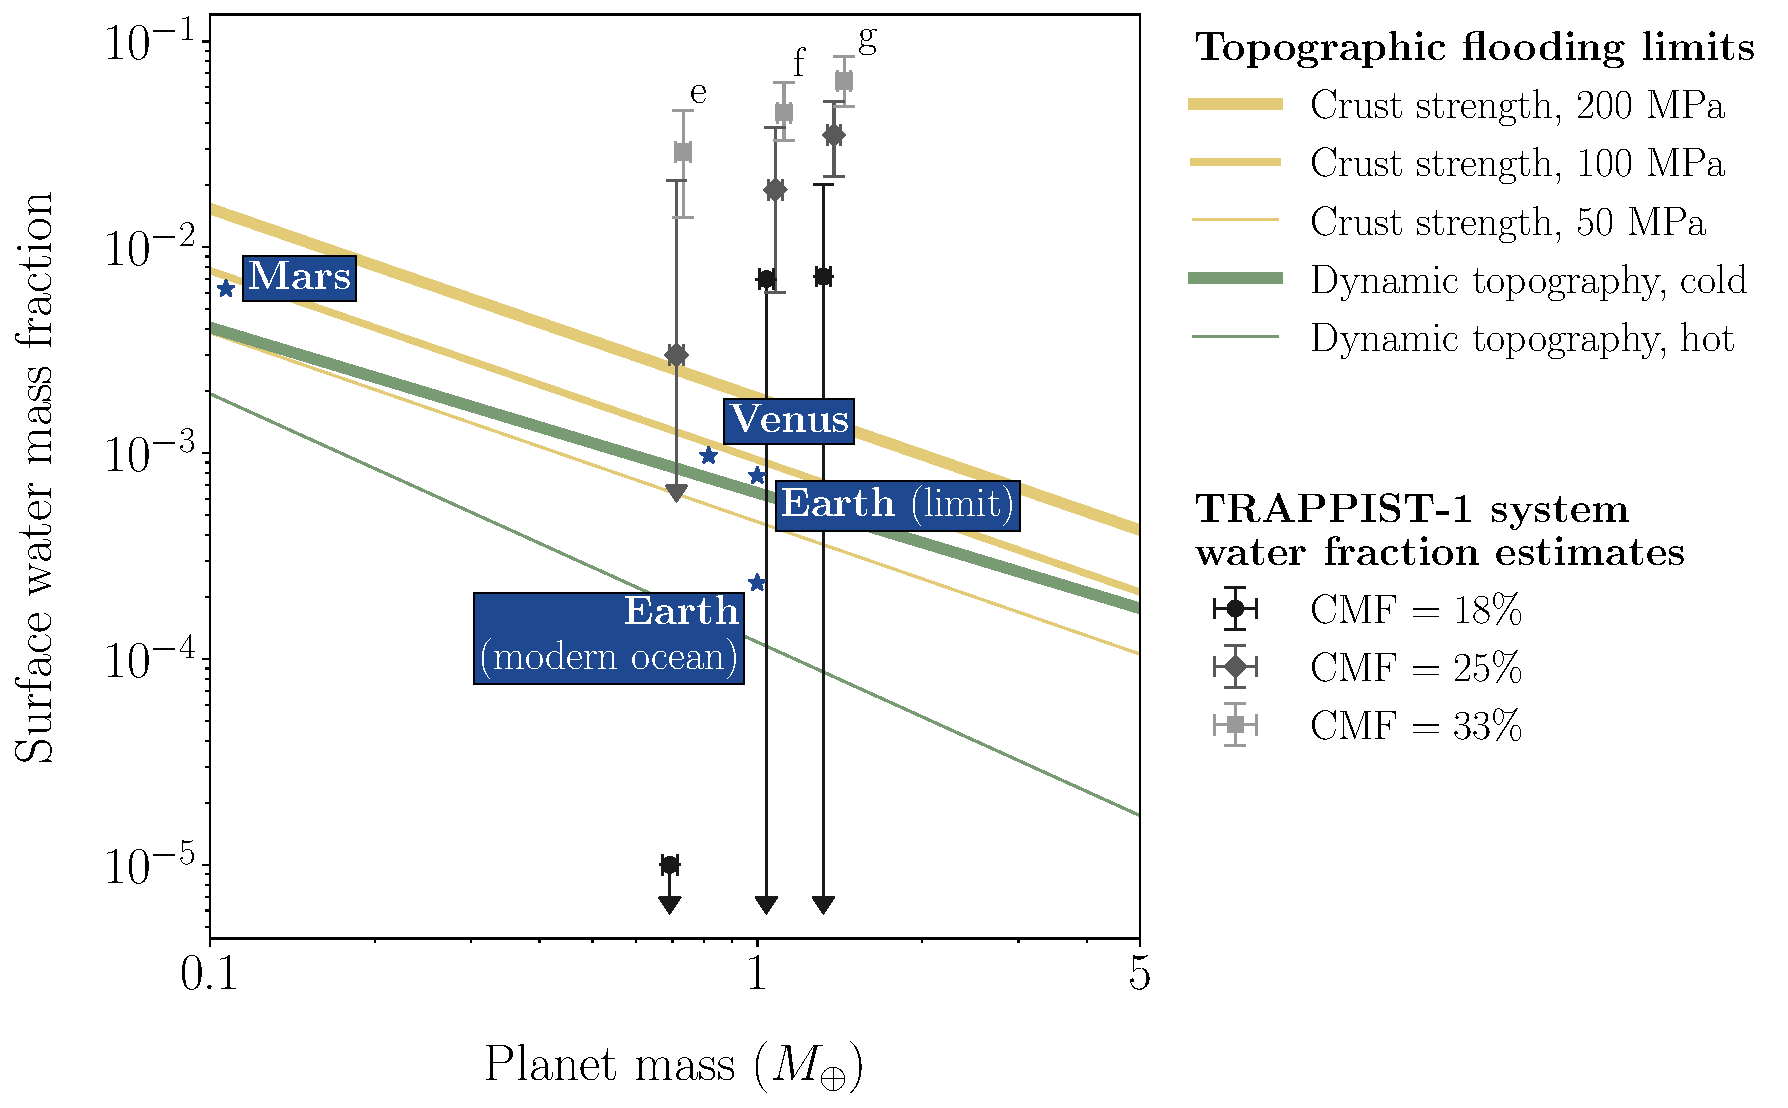
\includegraphics[width=\textwidth]{ww_lim.pdf}
    \caption[Various scalings for the maximum surface water capacity set by a planet's peak elevation.]{Various scalings for the maximum surface water capacity set by a planet's peak elevation, expressed as a fraction of the total planet mass. The yellow lines show the peak topography balanced by crustal rock strength alone, and scales approximately with $M_p^{-0.9}$; line widths correspond to different assumptions about the maximum strength with a fixed crust density of 2700~$\rm{kg\,m^{-3}}$. The thick green line shows pure dynamic topography with the coolest mantles considered, given a dry olivine rheology ($\propto M_p^{-0.8}$). The thin green line is the same for the hottest mantles ($\propto M_p^{-1.2}$). Scalings assume the mass-radius relation in (\ref{eq:MR}) and a red noise-like topographic spectral structure. Points with error bars are estimates of the surface water inventories of planets e--g in the TRAPPIST-1 system from \citet{agol_refining_2021}, for different possible values of the core mass fraction (CMF). Note that their analysis suggests cores most likely smaller than the Earth-like CMF of 33\%. Our thermal evolution model does not include tidal heating, which would push the TRAPPIST-1 planets towards higher mantle temperatures. For context, the labelled blue stars show the maximum ocean masses that could be contained on Venus, Earth and Mars, plus Earth's actual ocean mass.}
    \label{fig:max-ocn}
\end{figure}
 

\citet{agol_refining_2021} give preliminary constraints on the surface water content of the TRAPPIST-1 planetary system, for different values of the CMF and assuming all water exists as a condensed surface layer. Although the problem is degenerate, planets e--g appear consistent with water layers deeper than Earth's, on the order of at least 0.1\% of the planet mass. Other independent estimates have produced similar results \citep{acuna_characterisation_2021}.  %\citet{unterborn_inward_2018} also infer high water mass fractions for TRAPPIST-1f and g. 
This water budget would place TRAPPIST-1e to g well above the upper water mass limit for maintaining land with dynamic topography. Note, however, that the high rates of tidal heating inferred for some of these planets \citep{barr_interior_2018} would reduce dynamic topography beyond what is modelled here.

As we have previously emphasised, however, the true limit to elevation differences on a planet will be higher than that suggested by purely dynamic topography. To estimate a planet's total scope for land, we can calculate the minimum value of $h_{\rm peak}$ required for an instance of land on a planet with a given radius and surface water content. We find that any instance of land on TRAPPIST-1e would require a peak topographic amplitude of $\sim$40~km (a minimum RMS topography of $\sim$10~km), given 0.3 wt.\% surface water (\citeauthor{agol_refining_2021}'s estimate for a CMF of 0.25). Then one could compare this minimum to a rough estimate of the overall maximum elevation. %, taken to be the height of a surface load that would induce brittle failure in the crust.

In section 1 we motivated a crustal strength limit: for a surface load of $\rho g h$, somewhere in the crust below, at a depth of about 1/4 times the load width, a minimum stress difference $Y$ of 1/2 to 1/3 $\rho g h$ is sustained \citep{jeffreys_earth_1929}. This result assumes a flat earth model of elastic stress distributions, and holds for various load configurations of horizontal scale less than a few hundred kilometres. \citet{melosh_planetary_2011} illustrates that the force balance given by
\begin{equation}\label{eq:crust_strength}
    Y \approx 0.5 \rho_c g h,
\end{equation}
with a crust density $\rho_c = 2700$~$\rm{kg\,m^{-3}}$, and $Y$ set at an effective crustal strength on the order of 100 MPa, will roughly reproduce the maximum elevations of Venus, Earth, and Mars (Fig. \ref{fig:max-ocn}). Whilst this estimate is certainly an oversimplification, a more rigorous effort will naturally become very complicated, not the least due to the difficulty in predicting, from planetary bulk properties, a value of $Y$ corresponding to the maximum $h$.%large variation of empirical compressive strengths even for the same lithology. 
\nomenclature[a-y]{$Y$}{crustal strength [Pa]}

In typical crustal strength models, the strength increases with depth (lithostatic pressure) according to the rock's resistance to frictional sliding in the relatively cool, shallow part---the brittle regime---until viscosity is low enough to favour ductile deformation instead, and strength starts to decrease with depth (temperature). Thus the strongest part of the crust is near this brittle-ductile transition. However, the resulting strength maxima of $\sim$500~MPa or more for Earth-like conditions \citep{katayama_strength_2021} would imply $\sim$40 km of peak topography using (\ref{eq:crust_strength}); it is a limit not necessarily reached in practice. Further complicating the application of (\ref{eq:crust_strength}), crustal strength profiles are strongly sensitive to the temperature profile and porosity of the crust---generating these profiles for arbitrary exoplanets must attend to assumptions on these facets \citep{byrne_effects_2021}---and surface gravity has a nonlinear effect on brittle strength through its influence on porosity and fracture density \citep{heap_low_2017}. For example, doubling the thermal gradient will approximately halve the maximum $Y$---and thus $h$---in a dry case, and including hydrostatic pore fluid pressure shows a similar decrease \citep{katayama_strength_2021}.

A parallel approach to estimating maximum elevation differences from crustal concerns comes from isostasy. The height of a topographic feature above a plain is $h_A = (t_R - t_{\rm avg})(\rho_m - \rho_c)/\rho_c$, where $t_R$ is the thickness of the crust below the feature and $t_{\rm avg}$ is the average crustal thickness of the plain. For a basaltic crust (the primary crust formed from an Earth-like bulk composition), the maximum value of $t_R$ is set by the phase transition from basalt to denser and unstable eclogite: the crust cannot be much thicker than the depth of this transition. This fact limits the peak isostatic $h_A$ to about 15 km for a Venus-like case \citep{jull_implications_1995}. However, the depth of this phase transition depends sensitively on the crust thermal structure, and estimating $h_A$ in practice requires knowing $t_{\rm avg}$.

Finally, the height limits of volcanoes in particular must follow tighter rules. Magma will only rise to the top of a vent---and contribute to a growing pile of lava---so long as the vertical pressure gradient across the system is positive. \citet{castruccio_influence_2017} write this limit as $h_{\rm max} = (\Delta\rho/\rho_m) H + \Delta P_i/(\rho_m g)$, where $\Delta\rho$ is the density contrast between the crust and the magma, $H$ is the depth from the surface to the magma chamber, and $\Delta P_i$ is the critical overpressure to trigger an eruption (the pressure that would crack the magma chamber roof, related to the tensile strength of the crust and tellurically on the order of $\sim$20 MPa). Although a narrow range of $H$ can be argued for on Earth, related to the magma water content and crustal rheology \citep{huber_optimal_2019}, this concept has not yet been expanded to comparative planetology. 

In light of the above complexities, it is difficult to find a middle ground between the oversimplification of (\ref{eq:crust_strength}) using a universal crustal strength estimate, and a careful case-by-case application. %\citep[like those used to estimate topographically-loaded fault stresses in earthquake hazard regions; e.g.,][]{styron_weight_2015}. 
We will employ the former for the present purpose of comparing peak dynamic topography to peak total topography. We consider $Y = 100$ MPa, ostensibly representing the compressive strength of granite---the difference in compressive strength between an average granite and average basalt seems to be smaller than the spread seen across individual basalt samples in various laboratory conditions \citep{heap_low_2017}---but also include scalings for half and double this strength value.
%We do not try to constrain the available crustal strength as a function of planetary bulk properties, and simply show the maximum elevation that would be associated with an effective strength of 100 MPa \citep{melosh_planetary_2011).



% We can try to improve on our limit with the simplifying assumption that rocks will fracture at very small strains, and it is frictional sliding at faults which governs the effective crustal strength. This assumption is convenient because at high normal stresses, many different rock types follow a universal law for the shear stress to initiate sliding \citep{byerlee_friction_1978}. This shear stress increases with normal stress (depth) up until the point where the rock's resistance to ductile deformation becomes weaker than its resistnce to frictional sliding. Thus all planetary crusts might be expected to exhibit a peak strength just above this brittle-ductile transition. Without attention to the actual location of the maximum stress difference under the topographic load, which depends on its aspect ratio, we will na\"{i}vely say that the shear stress at the brittle-ductile transition is equal to the value of $Y$ at the maximum elevation. \todo{To this end, we can use brittle-ductile transition depths as a function of planetary parameters recently calculated by \citet{byrne_effects_2021}.........\n......}



%\todo{The highest topographic load that can be supported by the crust's own strength is $2Y/(\rho_c g)$, where $Y$ is the rock crushing strength ($\sim$100~MPa), $\rho_c$ is the crust density (2700~$\rm{kg\,m^{-3}}$), and $g$ is the surface gravity \citep[e.g.,][]{melosh_planetary_2011}. The factor of 2 comes from the distribution of stresses in the elastic half-space. --- explain that factor is kind of empirical but consistent with Jeffreys}


Fig. \ref{fig:max-ocn} plots the containable ocean mass fraction scalings corresponding to both this crust strength limit and to the dynamic topography limits calculated previously. For a given scaling relationship, points above the line would be waterworlds. We see that planet e may have coexisting land and water if its crust could withstand around 200 MPa of normal stress. Although these strengths can be achieved on Earth, it is not immediately obvious that they would available at the right loci.
% a minimum $h_{\rm peak}$ of 40~km for TRAPPIST-1e exceeds the theoretical peak elevation of $\sim$9.2~km at the crustal strength limit, using a surface gravity of 8.01~$\rm{m\,s^{-2}}$ (Fig. \ref{fig:max-ocn}). %Note that the actual topography could exceed this strength limit for a floating low-density crust \citep[c.f.][]{cowan_water_2014}, but the elevation gain depends on the unknown crust thickness. 
Note that it is very difficult in practice to put a lower limit on these water budgets. Nevertheless, according to \citet{agol_refining_2021}, TRAPPIST-1e through g could easily be wet enough that estimating their land propensities may seem moot. However, our growing catalogue of planets may soon present a case study closer to the waterworld-land world transition. %Regardless, the immense complexity of a real planet would prevent us from trying to seriously predict the height of topography on a given planet.

Another takeaway from Fig. \ref{fig:max-ocn} is that for the most massive rocky planets, amplitudes of dynamic topography in the most favourable case seem to approach the overall limit. Scalings for different internal heating scenarios have different slopes because, as surface heat fluxes increase with the surface area-to-volume ratio, larger planets are penalised such that any extra radiogenic heat would escape less easily. Thus more internal heating per unit volume in more massive planets will have a more drastic effect on topography. 


At the moment, it is not guaranteed that constraints on these or any rocky exoplanet water budgets could be tightened much in the future. With current Bayesian inference methods, uncertainties on retrieved water mass fractions may be capped at around $\sigma \approx 10$~wt.\%, independent of the observational uncertainty on the planet mass itself \citep{otegi_impact_2020}. Meanwhile, topography can avert waterworlds only for water mass fractions of $\lesssim 1$~wt.\%. Therefore, with respect to predictions about a given exoplanet, any topographic contribution to land coverage could be washed out by the uncertainty on the inferred water budget.


% \todo{[COPYING OLI'S COMMENT FROM LAST DRAFT:] How much uncertainty there is in water inventory for a planet that has an observational mass radius consistent with a dry rocky plane.  I.e., given the errors on the M-R observations, could we sneak a lot of waterworlds into the planet population if it wasn't for topography?}

% \todo{---CMG: This isn't an easy question to answer. \citet{dorn_bayesian_2017} have a whole paper on this and find, for a Neptune-like case, a retrieved surface water range of 22--50\% of $M_p$, with PLATO-like uncertainty in $M_p$ and $R_p$. Fig. \ref{fig:ocn-vol} shows that dynamic topography can be important at the 0.01\% water level in the best case scenario. So the answer is very likely no (we'd need to distinguish between e.g. 0.01\% and 0.05\% water mass fractions). Later, \citet{otegi_impact_2020} apply the same kind of analysis to find that for planets slightly less dense than Earth (i.e. something with an Earth-like core mass fraction but extra surface water), the uncertainty on the retrieve water mass fraction is basically insensitive to the data uncertainty, and is fixed at around $\sigma_{WMF}$ = 10 wt.\% for the most massive rocky planets.} 
 
% Considering the uncertainty there is on a planet's water inventory given measurements of its mass and radius, it may be important to consider topography in estimating the likelihood of a planet being a waterworld. The lowest-density end-member mass-radius relation can be constructed by assuming a low but nonzero planetary Fe/Mg ratio, with all the Fe existing in oxidised form in the mantle, so the planet has no metallic iron core \citep{unterborn_inward_2018}.  
 
% For an increasing fiducial core size, a higher allowable water mass fraction is needed to reproduce the observed bulk density. However, the measured mass and radii themselves have errors---this can result in a bulk density uncertainty of down to $\sim$150 $\rm{kg\,m^{-3}}$ \citep[for the TRAPPIST-1 system;][]{agol_refining_2021}, which corresponds to an uncertainty on the water layer thickness of \todo{XX} for an example coreless Earth-mass planet. This uncertainty is \todo{[higher/lower]} than the increase in land propensity one would get by considering the maximum topography required to create an infinitesimally small island. 


\subsection{Constraints from astrophysical data} \label{sec:obvs}

In Fig. \ref{fig:1D-h-scale}, we predicted how dynamic topography might vary as a function of several properties broadly deemed observable. None of these properties will be perfectly known, or even necessarily constrained well-enough such that they are not the dominant source of uncertainty, but we will leave a more detailed assessment of this uncertainty to future work.

In any case, an obvious fact emerging from our scaling law application is that there is a pivotal future role to be filled for any constraints on rocky planet compositions. This study provides yet another example of how higher-order properties of planetary interiors govern their surface character. Namely, mantle viscosities, radiogenic heating rates, and core mass fractions all relate to planetary ratios of certain major elements: viscosities decrease with Mg/Si, radiogenic heating rates increase with U/Si and Th/Si, and core mass fractions increase with Fe/O. Exoplanet compositional parameters are not completely inaccessible because refractory element ratios are expected to generally preserve themselves between a star and its planets \citep{thiabaud_elemental_2015, hinkel_star_2018, putirka_composition_2019, adibekyan_compositional_2021}. Although pilot work is surely needed, this useful fact means that element abundances from stellar spectra offer a promising constraint on planetary interior dynamics. Additionally, measurements of the same element ratios in polluted white dwarf spectra could inform the underlying natural distributions of bulk rocky planet composition across nearby star systems \citep{bonsor_hoststar_2021}. 

% We have already mentioned the link between bulk mineralogy and mantle rheology in section \ref{sec:discussion-rheology}. As for the CMF, relative abundances of Mg, Si, and Fe from a host star spectrum can also help somewhat to resolve degeneracies in planet interior structures; that is, the layer thicknesses of the iron core, silicate mantle, water/ice, and volatile envelope \citep{dorn_bayesian_2017, brugger_constraints_2017, schulze_probability_2020}. Early Monte Carlo estimates of the TRAPPIST-1 planets' interior structures are consistent with a constant composition across the entire system \citep{agol_refining_2021}. %From the mass balance of chondritic material, there is a theoretical maximum CMF of  $\sim$0.34 assuming no stripping of the silicate mantle \citep[see][]{dyck_effect_2021}, although Mercury demonstrates that the CMF can reach higher values in practice, and a handful of known exoplanets have measured bulk densities consistent with a mostly iron composition \citep{rappaport_roche_2013, toledo-padron_characterization_2020}.

%Element abundances from stellar spectra, in particular their abundances relative to silicate-forming Mg or Si, can also inform the internal heating budget of a planet \citep{unterborn_thorium_2015, botelhoThoriumSolarTwins2019, nimmo_radiogenic_2020, wang_europium_2020}. \citet{unterborn_thorium_2015} found Th abundances to vary two-fold in a sample of solar-twin stars. Th abundances relate to the planetary radiogenic heating rate at a given (stellar) age via nebular condensation models, combined with either measurements of U abundance in the same sample, or with the assumption that U and Th vary in the same way. 



% Abundances of Eu, which has stronger spectral features, may also be a convenient proxy for both Th and U abundances, since they are all synthesised in the $r$-process \citep{wang_europium_2020}. 

%Potassium-40 abundances as a function of heliocentric distance are more difficult to predict from stellar abundances because K would be volatilised during planetary formation processes.

Observables for exoplanetary topography itself would be buried quite deep. \citet{mctier_finding_2018} proposed that extreme topographic features could induce scatter in an exoplanet's transit photometry, but the associated signal would not be detectable with realistic photometric precision. Proposed next-generation direct imaging missions might be capable of enough precision for the exo-cartography of small planets---solving the inverse problem of 2D albedo distributions from time-resolved light-curves---which might discriminate between land and ocean surfaces \citep{cowan_mapping_2018, farr_exocartographer_2018, lustig-yaeger_detecting_2018, kawahara_global_2020, aizawa_global_2020}. Interpretations of the data may remain highly model-dependent and burdened by cloud removal, however \citep{paradise_fundamental_2021, teinturier_mapping_2022}. Ocean fractions might also be discerned from near-infrared polarimetric observations \citep{takahashi_polarimetric_2021}. A land fraction between zero and unity would necessitate some surface roughness, leading to an upper limit on the water budget given some inferences about topographic propensity. %Exo-cartography, or, solving the inverse problem of 2D albedo distributions from time-resolved light-curves,  %Ocean glint (specular reflection) might also leave a characteristic signal in the observations of a transiting or directly-imaged planet \citep{robinson_2010_detecting, robinson_2014_detection, lustig-yaeger_detecting_2018}. 



% \todo{[anything useful from the solar system?]}

% \todo{look at the weathering work from \citet{krissansen-totton_constraining_2017}, \citet{lehmer_carbonate-silicate_2020}, jade checlair... any difference in atmospheric co2 if all weathering is suboceanic, considering statistical variation of other important factors, and would this be measurable with e.g. luvoir? could exocartography distinguish between waterworlds and ``marbles"? check \citet{rushby_effect_2019} on total albedo differences---they say the signal would probably not be detectable in transit. in principle if you were pretty sure a planet was not a waterworld from observations then what would Fig. \ref{fig:ocn-vol} tell you.. }


\section{Conclusions}

This work has predicted scaling relationships for the RMS amplitude of dynamically-supported topography on stagnant lid planets, which we propose to be a deterministically-tractable aspect of rocky exoplanet surface character. We find RMS topography to decrease strongly with higher interior temperatures and lower mantle viscosities. Planets near the upper mass-limit of rockiness would thus have inconsequential dynamic topography, as would planets with radioisotope abundances several times that of Earth. For planets less than about twice the mass of Earth, our thermal history model predicts RMS dynamic topography on the order of hundreds of metres. This result emphasises that modelling purely dynamic topography will underestimate a planet's true RMS elevation. A robust upper limit to total topography may be limited by our ability to predict crustal thicknesses.

Considering that dynamic topography is guaranteed to exist on active planets, however, the model can be used to infer, with strong caveats, whether subaerial land exists on a planet for a given surface water budget. We define the ocean basin capacity as the volume of water that could be contained below the highest elevation. As planet size increases, interior temperatures and surface gravity increase and topography shrinks, but the available storage of the ocean basins expands with the surface area. These effects nearly cancel out at Earth-like radiogenic heating rates, leading to a constant ocean basin capacity of about 0.3 Earth oceans if topography is dynamically-supported alone. For a 1-$M_\oplus$ planet this translates to a maximum surface water mass fraction of $\sim$60~ppm before the planet has no land above sea level. The same water budget would flood more massive planets. In reality, volcanic construction would lead to higher surface relief than that from dynamic topography alone---in modelling only the latter, we are providing a lower limit, or ``worst-case scenario," of the true ocean basin capacity. To avert waterworlds on high mass planets, other sources of topography would be vital.


% The unconstrained rheology of the mantle (a function of its bulk composition and water content) represents an important source of uncertainty on RMS topography predictions. Improved estimates of mantle rheology based on mineralogy models will be a key future pursuit in the exogeosciences.


% We have presented the first deterministic geophysical model of large-scale topography applied to rocky exoplanets. Our initial investigation has been limited to dynamic topography on stagnant lid planets, and even in this context has necessitated simplifications. Lithospheric elastic filtering and erosion would both decrease the height of dynamic topography from that reported here, whilst associated magmatism would increase it.

% Descriptive mathematical  \citep{ermakov_power_2018, landais_multifractal_2019}, while invaluable, are not designed to show how the dimensional amplitudes of topography might depend on geophysical processes in a deterministic sense. There exists a knowledge gap between how to predict topographic amplitudes and how to describe their distributions. Whilst here we have focussed on the former side, we have also presented a primitive attempt at bridging pattern and process by \todo{...................}

A useful waypoint from this work is a naive scaling relationship of RMS dynamic topography in terms of the mantle Rayleigh number and viscosity contrast, for chaotic time-dependent convection with large viscosity contrasts. Our results suggest a weaker Ra-dependence and overall higher topography amplitudes compared to the isoviscous convection scalings previously reported. %The rigour of our bespoke scaling is somewhat limited by the available CPU time, and we encourage dedicated future work on the topic. \todo{I mean that we aren't able to produce a high=res grid to see the bifurcations, also test different initial conditions...}
 





Segments of the general approach here might guide other mysteries about rocky planet surface architecture---which seems, at the time of writing, an unpopulated but fertile field of research. We conceive of a framework into which new geophysical or geomorphological models could easily slide. Particularly, the method of gauging whole surface layouts via the RMS amplitude extends to other ways of generating large-scale topography, so long as---and this step is nontrivial---one could write process-based scaling laws for how its RMS value changes with planetary bulk properties. Reasonable assumptions about the power spectral distribution of topography give peak amplitudes between 3.5 and 3.9 times the RMS value, consistent across different ways of supporting loads. With that said, care should be taken to not overemphasise the general feasibility of such applications, given that decades of examination into our own planet's topography have not yet reached any steadfast deterministic rules. To push the marriage between these sciences further \citep{shorttle_why_2021}, then, finding tighter links between pattern and process on the surface of Earth will be paramount to understanding how landscapes manifest on billions of rocky planets in the universe.



\subsection*{Acknowledgements}

We acknowledge the support of the University of Cambridge Harding Distinguished Postgraduate Scholars Programme and the Natural Sciences and Engineering Research Council of Canada (NSERC). Cette recherche a \'{e}t\'{e} financ\'{e}e par le Conseil de recherches en sciences naturelles et en g\'{e}nie du Canada (CRSNG). We thank the Computational Infrastructure for Geodynamics (geodynamics.org) which is funded by the National Science Foundation under award EAR-0949446 and EAR-1550901 for supporting the development of ASPECT.






%\nomenclature[z-DEM]{DEM}{Discrete Element Method}
%\nomenclature[z-FEM]{FEM}{Finite Element Method}
%\nomenclature[z-PFEM]{PFEM}{Particle Finite Element Method}
%\nomenclature[z-FVM]{FVM}{Finite Volume Method}
%\nomenclature[z-BEM]{BEM}{Boundary Element Method}
%\nomenclature[z-MPM]{MPM}{Material Point Method}
%\nomenclature[z-LBM]{LBM}{Lattice Boltzmann Method}
%\nomenclature[z-MRT]{MRT}{Multi-Relaxation Time}
%\nomenclature[z-RVE]{RVE}{Representative Elemental Volume}
%\nomenclature[z-GPU]{GPU}{Graphics Processing Unit}
%\nomenclature[z-SH]{SH}{Savage Hutter}
%\nomenclature[z-CFD]{CFD}{Computational Fluid Dynamics}
%\nomenclature[z-LES]{LES}{Large Eddy Simulation}
%\nomenclature[z-FLOP]{FLOP}{Floating Point Operations}
%\nomenclature[z-ALU]{ALU}{Arithmetic Logic Unit}
%\nomenclature[z-FPU]{FPU}{Floating Point Unit}
%\nomenclature[z-SM]{SM}{Streaming Multiprocessors}
%\nomenclature[z-PCI]{PCI}{Peripheral Component Interconnect}
%\nomenclature[z-CK]{CK}{Carman - Kozeny}
%\nomenclature[z-CD]{CD}{Contact Dynamics}
%\nomenclature[z-DNS]{DNS}{Direct Numerical Simulation}
%\nomenclature[z-EFG]{EFG}{Element-Free Galerkin}
%\nomenclature[z-PIC]{PIC}{Particle-in-cell}
%\nomenclature[z-USF]{USF}{Update Stress First}
%\nomenclature[z-USL]{USL}{Update Stress Last}
%\nomenclature[s-crit]{crit}{Critical state}
%\nomenclature[z-DKT]{DKT}{Draft Kiss Tumble}
%\nomenclature[z-PPC]{PPC}{Particles per cell}
%
%
%
%\nomenclature[z-cif]{$CIF$}{Cauchy's Integral Formula}                                % first letter Z is for Acronyms 
%\nomenclature[a-F]{$F$}{complex function}                                                   % first letter A is for Roman symbols
%\nomenclature[g-p]{$\pi$}{ $\simeq 3.14\ldots$}                                             % first letter G is for Greek Symbols
%\nomenclature[g-i]{$\iota$}{unit imaginary number $\sqrt{-1}$}                      % first letter G is for Greek Symbols
%\nomenclature[g-g]{$\gamma$}{a simply closed curve on a complex plane}  % first letter G is for Greek Symbols
%\nomenclature[x-i]{$\oint_\gamma$}{integration around a curve $\gamma$} % first letter X is for Other Symbols
%\nomenclature[r-j]{$j$}{superscript index}                                                       % first letter R is for superscripts
%\nomenclature[s-0]{$0$}{subscript index}                                                        % first letter S is for subscripts


%!TEX root = ../thesis.tex
%*******************************************************************************
%****************************** Second Chapter *********************************
%*******************************************************************************

\chapter[Low volcanic outgassing rates for a stagnant lid Archean Earth]{Low volcanic outgassing rates for a stagnant lid Archean Earth with graphite-saturated magmas}
\label{chapter:outgassing}

\ifpdf
    \graphicspath{{Chapter2/Figs/Raster/}{Chapter2/Figs/PDF/}{Chapter2/Figs/}}
\else
    \graphicspath{{Chapter2/Figs/Vector/}{Chapter2/Figs/}}
\fi


%\section[Short title]{Reasonably long section title}

% Uncomment this line, when you have siunitx package loaded.
%The SI Units for dynamic viscosity is \si{\newton\second\per\metre\squared}.


%\usepackage[normalem]{ulem}
\newcommand{\Ncases}{762}

\section*{Preface}

This chapter was published under the same title in \textit{Physics of the Earth and Planetary Interiors} in November 2021, appearing in the bibliography as \citet*{guimond_low_2021}. After a short note on author contributions, it is presented here reformatted, but otherwise unaltered, excepting minor notation changes for consistency with the rest of the thesis.


\subsubsection*{Contributions and context}

%Unlike the other chapters, the work here is not coauthored by my PhD supervisors. 
This project begun before moving to Cambridge, whist I was a Gastwissenschaftlerin at the Freie Universit\"at Berlin in early 2019. It was conceived of by Lena Noack, who coauthored the article and served as my advisor at FUB. During my 7 months there, I generated the model data that went into the original submitted manuscript and produced the first draft. However, a lengthly review process meant that much of results were re-analysed, and the manuscript re-written, during the first two years of my PhD. I chose incidentally to include this work here because, as a focussed study of early Earth, it is a good complement to the broader studies of fiducial rocky exoplanets presented in the other chapters. Besides Lena, I acknowledge the article's other coauthors Gianluigi Ortenzi and Frank Sohl for contributing the volatile speciation model used in this study. Note that a sibling article, \citet{ortenzi_mantle_2020} of which I am also a coauthor, extends some of these results to rocky planets in general.


\section*{Abstract}
Volcanic gases supplied a large part of Earth's early atmosphere, but constraints on their flux are scarce. Here we model how C-O-H outgassing could have evolved through the late Hadean and early Archean, under the conditions that global plate tectonics had not yet initiated, all outgassing was subaerial, and graphite was the stable carbon phase in the melt source regions. The model fully couples numerical mantle convection, partitioning of volatiles into the melt, and chemical speciation in the gas phase. The mantle oxidation state (which may not have reached late Archean values in the Hadean) is the dominant control on individual species' outgassing rates because it affects both the carbon content of basaltic magmas and the speciation of degassed volatiles. Volcanic gas from mantles more reduced than the iron-w\"ustite mineral redox buffer would contain virtually no CO$_2$ because (i) carbonate ions dissolve in magmas only in very limited amounts, and (ii) almost all degassed carbon takes the form of CO instead of CO$_2$. For oxidised mantles near the quartz-fayalite-magnetite buffer, we predict median CO$_2$ outgassing rates of less than approximately 5 Tmol yr$^{-1}$, still lower than the outgassing rates used in many Archean climate studies. Relatively weak outgassing is due in part to the redox-limited CO$_2$ contents of graphite-saturated melts, and also to a stagnant lid regime's inefficient replenishment of upper mantle volatiles. Our results point to certain chemical and geodynamic prerequisites for sustaining a clement climate with a volcanic greenhouse under the Faint Young Sun.



\section{Introduction}

The Hadean-Archean atmosphere cloaked the only environment in the universe known to support the origin of life. This atmosphere would have been fed by volatile chemicals outgassed from the interior \citep{Holland1984, kasting_mantle_1993, gaillard_theoretical_2014}, as well as extraterrestrial impacts \citep{Zahnle2020} and perhaps a lingering, degassed magma ocean atmosphere \citep{katyal_effect_2020}. Yet hardly any observable record of the Archean atmosphere remains. Our knowledge surrounding its makeup rests on modelling. Mantle outgassing models lend boundary conditions to the processes controlling the atmospheric composition and planetary climate. However, predictions from these models are very much entwined with certain assumptions---in particular, the tectonic regime and oxidation state of the mantle. Archean outgassing scenarios hinging on mobile plates and an oxidised mantle form the basis of contemporaneous climate studies \citep[e.g.,][]{Sleep2001}. This work offers an alternative to these recurring premises: a fully-coupled numerical estimation of the volcanic outgassing rates of \ch{CO2}, \ch{CO}, \ch{H2O}, and \ch{H2}, for a stagnant lid Earth under a range of mantle oxidation states. 

The oxidation state of the upper mantle controls the chemical speciation of volcanic gas. Increasing the mantle's oxygen fugacity, $f_{\rm O_2}$, raises the ratio of oxidised to reduced volatile species in the melt phase: [\ch{CO2}]/[\ch{CO}] and [\ch{H2O}]/[\ch{H2}] in the C-O-H system \citep{Holland1984}. As the melt rises adiabatically through conduits, its $f_{\rm O_2}$ re-equilibriates with the decreasing pressure; gas abundances at the surface are also linked to the mantle source region \citep{kasting_mantle_1993}. On modern Earth, for example, the dominant species in volcanic gas are \ch{H2O} and \ch{CO2}, in line with a mantle source $f_{\rm{O_2}}$ in equilibrium with the quartz-fayalite-magnetite (FMQ) mineral buffer \citep{Holland1984}. 

Besides the effect of $f_{\rm{O_2}}$ on volatile speciation, there can be a compounding redox control on the partitioning of carbon into the melt. This effect becomes relevant when graphite is the stable carbon phase in the upper mantle. During melting, carbonate ions are produced from a reaction of graphite with oxygen via \ch{CO2} \citep{holloway_highpressure_1992}. The total carbon outgassing flux depends on how much carbon (as \ch{CO3^{2-}}) can dissolve into the melt. 

Although these two redox effects are well-known, the value itself of the Archean mantle $f_{\rm O_2}$ remains weakly constrained at best. Immediately after core formation, the magma ocean must have been reduced \citep{Wood2006}. Meanwhile, scant geological evidence suggests that by $\sim$3.8~Ga at the latest, the uppermost mantle was already about as oxidised as today \citep{Canil1997, Delano2001, Trail2011, NICKLAS2019, Armstrong2019}. Yet uncertainty persists on the timing of this oxidation (see section \ref{sec:redox}). Therefore, to cover the possible spread of redox states, we investigate outgassing fluxes under a wide range of mantle $f_{\rm O_2}$, especially in proportion to other unknown parameters such as the mantle volatile content and thermal state.

Whilst this study is set up to explore many redox scenarios, it will be limited to one tectonic regime. For this we consider the end-member case of stagnant lid convection \citep{Debaille2013}. The possibility of a stagnant lid regime appears underexplored in early Earth climate studies, despite the ambiguity around plate tectonics' operation through the Archean \citep[e.g.,][]{Brown2020}; as such we hope to complement other work assuming a mobile lid. This modelling decision is important because mobile lids may be associated with much higher outgassing rates than stagnant lids \citep{noack2014can, noack_volcanism_2017}. The mechanistic explanations are not straightforward---being a combination of competing effects discussed later in section \ref{sec:stagnant-lid}---and would benefit from dedicated work in the future.

By numerically coupling mantle convection, redox-dependent melt partitioning of volatiles, and redox-dependent speciation, and by investigating a broader range of mantle oxidation states, we can advance the current literature dedicated to C-O-H outgassing from solid-state mantles of rocky planets in the solar system and elsewhere \citep{ONeill2007,Grott2011,noack2014can,noack_volcanism_2017,tosi_habitability_2017,dorn_outgassing_2018, ortenzi_mantle_2020}. Previous studies have tended to assume an oxidising mantle, akin to that of present-day Earth---exceptions include \citet{Grott2011} for the reduced early Mars, and \citet{tosi_habitability_2017}, \citet{ortenzi_mantle_2020}, and \citet{Liggins2020} for fiducial rocky exoplanets. %We apply our model to Archean Earth, a case which has not yet been the dedicated subject of a C-O-H numerical outgassing study.
Further, numerical convection carries the advantage of resolving the local temperatures and pressures of melt parcels, to which $f_{\rm O_2}$ is very sensitive. 

An approach parallel to the one taken here is to parameterise outgassing fluxes in terms of melt production \citep[e.g.,][]{Sleep2001, Papuc2008, kite2009geodynamics, Kadoya2015, Foley2016, CHARNAY2017, KT2018, foley_carbon_2018, Krissansen-Totton2020}. In parameterised models, mantle melting rates are often scaled to an estimate of the interior heat flux. Past outgassing rates can then be calibrated to present-day estimates. These types of outgassing parameterisations may imply higher outgassing fluxes than do numerical convection models for two reasons. Firstly, heat flow scalings extrapolated backwards in time will necessarily lead to higher-than-modern outgassing rates because parameterised thermal history models predict high heat flow early in a planet's evolution \citep[e.g.,][]{TURCOTTE1980}. Secondly, 1D models tend to overestimate melt fractions early in a planet's thermal evolution, since they cannot spatially resolve depletion upon partial melting---local depletion would inhibit further local melting for the same temperature. In addition to these systematic effects, applying a single scaling relationship assumes no change in mantle oxidation state or tectonic regime.




Planetary outgassing rates require attention because they lie at the core of at least two unsolved Archean mysteries. The first is that reduced gases such as \ch{H2} and \ch{CO} may be necessary for prebiotic chemistry. The production of HCN requires a reducing atmosphere with C/O $\geq$ 1, for example \citep{Rimmer2019}. However, whether \ch{H2} and \ch{CO} could have comprised a significant part of volcanic gas at the time remains debated \citep[e.g.,][]{Zahnle2020}. The second mystery is that sufficiently large partial pressures of greenhouse gases seem required to incubate early Earth under lower solar luminosity \citep{charnay2020} and make sense of liquid surface water \citep{Sagan1972}. Although no solution to this paradox has emerged as the likely favourite, most atmospheric evolution scenarios proposed so far rely on \ch{CO2} outgassing fluxes at least as high as the present day \citep[e.g.,][]{Sleep2001, Wordsworth2013, KANZAKI2018}. Neither of these two driving questions may ever be resolvable without definite constraints on the timing of mantle oxidation, or plate tectonics' initiation. Nevertheless, this study, by more rigorously linking stagnant lid outgassing fluxes to the unknown oxidation state, might help contextualise these problems within Earth system evolution.





%%%%%%%%%%%%%%%%%%%%%%%%
\section{Methods}

We trace the movement of volatiles through the mantle to the atmosphere for a stagnant-lid Earth, from just after the moon-forming impact to around the first rock record. Our model is similar to the one described in \citet{ortenzi_mantle_2020}, who additionally calculated gas solubility in the melt (relevant for the higher outgassing pressures expected on exoplanets greater than an Earth mass), but coupled partitioning and volatile speciation \textit{a posteriori} within the convection simulations, rather than directly.


To simulate mantle dynamics, we use a 2D convection model, which is detailed in \citet{noack2016modeling}. The heavily-benchmarked model couples solid-state convection in the mantle with spatially-resolved melt fractions and volatile partitioning in the melt \citep{holloway_highpressure_1992, katz_new_2003, Grott2011}. This is further coupled with a chemical speciation model \citep{French1966, Holloway1981, Fegley2013, gaillard_theoretical_2014, schaefer_redox_2017}. At each time step the model produces outgassed masses of \ch{H2O}, \ch{H2}, \ch{CO2}, and \ch{CO}. We simulate 700~Myr of convection, with time-zero nominally corresponding to 4.5~Ga.



\subsection{Numerical convection model}

The convection code solves the conservation equations of mass, momentum and energy in the rocky mantle by using a particle-in-cell method. We use the 2D spherical annulus method in \citet{HERNLUND2008} to divide the mantle into a mesh of cells with an average lateral and radial resolution of 50 km between grid points. The radial resolution coarsens linearly with depth, varying from 10 km at the surface to 90 km at the core-mantle boundary. To reduce computational costs, we model one quarter of the 2D annulus, corresponding to 307 cells in the lateral direction. We found that minor changes in resolution did not affect degassing.

We model compressible convection based on the truncated anelastic liquid approximation (TALA), using pre-calculated depth-dependent profiles for thermodynamic parameters such as the mineral-dependent density, the thermal expansion coefficient and the heat capacity for an adiabatic temperature profile. We neglect any possible initiation of plate tectonics or other surface recycling mechanisms and instead allow for a stagnant lid to form. 

We take into account time-dependent radiogenic heating and heat loss from the core. The radiogenic heat sources decline over time and would reach present-day Earth values of 79.5 ppb Th, 240 ppm K and 20.3 ppb U after 4.5 Gyr of thermal evolution, following \citet{schubert_turcotte_olson_2001}.\footnote{Note that the values used in this Chapter for Bulk Silicate Earth's Th, K, and U concentrations are slightly different, by a few ppb, to those considered in Chapter \ref{chapter:topography}.} We did not include the partitioning of heat sources in the crust, and instead applied homogeneous radiogenic heat sources over the entire domain.

We assume a hydrated pyrolitic mantle with an Arrhenius viscosity, $\eta$, that depends on the local temperature $T$ and pressure $P$, following \citet{karato_rheology_1993}:
\begin{equation}
    \eta(T,P) = \frac{1}{2 A} d^r \exp\left(\frac{E_a+PV_a}{R_bT}\right),
\end{equation}
\nomenclature[a-dr]{$d^r$}{grain size [mm] with exponent in Arrhenius viscosity law}
\nomenclature[a-v]{$V_a$}{activation volume in Arrhenius viscosity law [${\rm cm}^{3}\,{\rm mol}^{-1}$]}
with, for the upper mantle, a prefactor $A=3.7 \times 10^{-19}\,{\rm m}^{-r}\,{\rm Pa}^{-1}\,{\rm s}^{-1}$, grain size $d=1\,{\rm mm}$, grain size exponent $r=2.5$, activation energy $E_a=240\,{\rm kJ}\,{\rm mol}^{-1}$, and activation volume $V_a=5.0\,{\rm cm}^{3}\,{\rm mol}^{-1}$, where $R_b$ is the gas constant. The lower mantle rheology behaves as in \citet{noack_volcanism_2017}, with a viscosity prefactor and pressure-dependent activation enthalpy following \citet{tackley_mantle_2013}; that is, $V_a$ decreases with pressure in the lower mantle. Whereas \citet{tackley_mantle_2013} increased their viscosities by a factor of 100 to allow for numerically-feasible simulations, we do not also adopt this scale factor, so the lower mantle is less viscous compared to their study.

Whilst we model a wet mantle, we do not consider local viscosity variations due to heterogeneous water contents. We do not implement an aesthenosphere, and may underestimate the convective strength locally in the upper mantle. Our initial Rayleigh number, estimated for a global average viscosity of about $10^{21}\,{\rm Pa\,s}$, is around $5\times10^7$. However, depending on the initial temperature profile and its local variations, the viscosity can be much lower than this---especially in the upper mantle---permitting more vigorous convection in some regions.



\subsection{Melting model}
The petrological model simulates partial melting of the silicate mantle. Melt forms if the local temperature is greater than the mantle solidus temperature, $T_{\rm solidus}$, at that temperature and pressure. The local melt fraction, $F$, is
\begin{equation}\label{eq:melt-fraction}
    F = \frac{T - T_{\rm solidus}}{T_{\rm liquidus} - T_{\rm solidus}}.
\end{equation}
\nomenclature[a-f]{$F$}{melt fraction}
The solidus and liquidus parameterisations, given in \citet{noack2014can}, are fits to experimental data for peridotite melting valid up to 15~GPa \citep{smet1999evolution}. The liquidus temperature, $T_{\rm liquidus}$, is constant for a given pressure. The solidus temperature decreases with water content in the melt \citep{katz_new_2003}, and increases upon depletion due to prior melting. Melting also consumes latent heat, feeding back into the local mantle temperatures. We assume that the upper mantle melt is buoyant only at pressures of less than 12~GPa \citep{ohtani_melting_1995}, hence we neglect any contribution from melting at greater depths. 

The local melt fractions add up to give the total chemical depletion of the mantle. Here, depletion is adapted to the fact that dehydration increases the solidus temperature. We recalculate the depletion at each time step using the updated solidus temperature. Upon 30\% depletion of the primordial peridotite mantle, the residual mantle therefore always resembles the harzburgite composition, independently of if it having started wet or dry. Depletion is limited to 30\%. We do not consider density variations in the mantle residue upon melting; that is, there is no buoyancy effect due to depletion.



\subsection{Volatile partitioning model}\label{sec:partitioning-methods}

At each time step, if the local melt fraction is greater than zero, we calculate the amounts of C and \ch{H2O} that enter the melt phase, and subtract them from the local chemical inventories. These inventories (as well as other local information such as the depletion) are traced via mass-independent particles that flow along convective stream lines. We ensure that each cell, which is fixed in space, has between 3 and 8 particles. No local partitioning occurs once a particle's volatile inventory is emptied; if a particle is dehydrated, it remains so. As the mantle convects, however, cells can be replenished by fresh particles rising up from the lower mantle, which replace the dehydrated particles. 

Carbon dissolves into the melt as \ch{CO3^2-}; its mole fraction, $X_{\ch{CO3^2-}}^{\rm melt}$, depends strongly on $f_{\rm O_2}$:
\begin{equation}\label{eq:c_partition}
    X_{\ch{CO3^2-}}^{\rm melt} = \frac{K_{\rm I} \, K_{\rm II} \, f_{\ch{O2}}}{1+K_{\rm I} \, K_{\rm II} \, f_{\ch{O2}}},
\end{equation}
where $K_{\rm I}$ and $K_{\rm II}$ are the equilibrium constants governing, respectively, the formation of \ch{CO2} from graphite and \ch{CO3^{2-}} from \ch{CO2},
\begin{align}
    \log K_{\rm I} &= a - b \, T + c \, T^2 + d \, \frac{p-1}{T}\\ 
    \log K_{\rm II} &= e - \frac{f}{T} - g \frac{P-1000}{T},
\end{align}
where $a = 40.07639$, $b = 2.53932\times 10^{-2}$, $c = 5.27096\times 10^{-6}$, $d=0.0267$, $e = -6.24763$, $f=282.56$, $g=0.119242$, $T$ is in K, and $P$ is in bar \citep{holloway_highpressure_1992, Grott2011, Hirschmann2008}. 

The weight fraction of \ch{CO2}, here denoted $\chi$ to distinguish from mole fraction, is calculated from $X_{\ch{CO3^2-}}^{\rm melt}$, assuming thermodynamic equilibrium:
\begin{equation}\label{eq:c_partition2}
    \chi_{\ch{CO2}}^{\rm melt} = \left. \left[\frac{M_{\ch{CO2}}}{\rm FWM} \, X_{\ch{CO3^2-}}^{\rm melt} \right] \; \middle/ \; \left[ 1 - \left(1-\frac{M_{\ch{CO2}}}{\rm FWM} \right) X_{\ch{CO3^2-}}^{\rm melt}\right] \right. ,
\end{equation}
where $M_{\ch{CO2}}$ is the molar mass of carbon dioxide in ${\rm g\,mol}^{-1}$ and FWM is the formula weight of the melt normalised to one oxygen, equal to $36.594\,{\rm g \, mol}^{-1}$ for an example tholeiitic basaltic \citep{holloway_highpressure_1992, Grott2011}. The formula weight typically varies only by few percent for different basalt compositions. Note that although (\ref{eq:c_partition}--\ref{eq:c_partition2}) do not directly involve the mantle source concentration, $\chi_{\ch{CO2}}^{\rm melt}$ is capped at the source concentration locally.

We make the simplifying assumption that all solid carbon exists as graphite in our application of \eqref{eq:c_partition}. In reality, diamond will be stable over graphite at pressures \textgreater5 GPa for the $P$--$T$--$f_{\rm O_2}$ we consider, and carbide will be stable throughout at $f_{\rm O_2} < {\rm IW}$ \citep[e.g.,][]{shirey_diamonds_2019}, so the solid-melt partitioning model we use will not accurately predict $X_{\ch{CO3^2-}}^{\rm melt}$ for the deepest melting and the most reduced cases. This assumption also may not be valid for the most oxidised cases (IW~+~4), as carbonate may become the stable carbon species for these pressures and $f_{\rm O_2}$ \citep{Stagno2019}. However, in such oxidised conditions we already know that \ch{CO2} is outgassed, and neglect any carbonate stability.

For water partitioning, we use the batch melting formula:
\begin{equation}\label{eq:h_partition}
    \chi_{\ch{H2O}}^{\rm melt} = \frac{\chi_{\ch{H2O}}^{\rm rock}}{D_{\ch{H2O}}+F(1-D_{\ch{H2O}})},
\end{equation}
where $\chi_{\ch{H2O}}^{\rm rock}$ is the local weight fraction of water in the solid mantle, $F$ is the local average melt fraction, and $D_{\ch{H2O}}$ is a partition coefficient, which we set at 0.01 based on the Ce partitioning coefficient \citep{MICHAEL1995, katz_new_2003}. 


Whilst the melt rises adiabatically towards the surface, we only allow a fixed fraction of the melt, $\chi_{\rm extr}$, to reach the surface as extrusive volcanism. Only this extrusive melt contributes to outgassing into the atmosphere. The mantle volatile concentrations are small enough to not saturate \citep{katz_new_2003}. We do not consider submarine degassing, so virtually all gas molecules enter the atmosphere at these lower surface pressures. Our model therefore assumes complete outgassing of the melt that reaches the surface, with no residual volatiles remaining in the melt. Finally, we do not consider any possible re-equilibration or contamination as material rises through the lithosphere, and neglect whether the melt interacts with the surrounding rock or with fluids at higher pressures.

\nomenclature[g-xmelt]{$\chi_{\rm H_2O}^{\rm melt}$}{melt H$_2$O concentration by weight}
\nomenclature[g-xmelt]{$\chi_{\rm CO_2}^{\rm melt}$}{melt CO$_2$ concentration by weight}

\subsection{Volatile speciation model}\label{sec:speciation-methods}


\begin{table}
\caption{Thermodynamic parameters for basaltic melt used in the outgassing model.
\label{table:thermo_param}}  
\centering   
\footnotesize
\begin{tabular}{l p{5cm} r l l}
\toprule   
\noalign{\vskip 1mm}   
 Symbol & Description & Value & Units & Reference \\    
\midrule     
\noalign{\vskip 1mm}   
   $\alpha_{\rm melt}$ & Thermal expansion coefficient & $3\times10^{-5}$ & K$^{-1}$ & \citet{Afonso2005} \\     
   $\rho_{\rm melt}$ & Density &  3000 & kg m$^{-3}$ & \citet{Lesher2015}\\
   $c_{p,{\rm melt}}$ & Heat capacity & 1793 & J kg$^{-1}$ K$^{-1}$ & \citet{Lesher2015} \\
\bottomrule                                  
\end{tabular}
\end{table}

We retrieve the masses of outgassed volatiles using the ``Equilibrium constants and mass balance method" first appearing in \citet{French1966}, and used widely in other studies \citep{Holland1984, gaillard_theoretical_2014, Fegley2013, schaefer_redox_2017, ortenzi_mantle_2020}. The [H$_2$]/[H$_2$O] and [CO]/[CO$_2$] molar ratios are governed by the chemical equilibria,
\begin{equation}\label{equilibrium_H2O}
    \ch{2 H2 +  O2 <=> 2 H2O},
\end{equation}
\begin{equation}\label{equilibrium_CO2}
    \ch{CO + (1/2) O2 <=> CO2},
    \end{equation}
assuming that the volcanic gases are in equilibrium with their magmas. These chemical reactions have respective equilibrium constants $K_{\rm III}$ and $K_{\rm IV}$, which are calculated as follows:
\begin{equation}\label{eq:equilibrium_constant_hydrogen}
   {K_{\rm III}}  = \exp\left(\frac{-\Delta G^0_{(\ref{equilibrium_H2O})} }{R_bT}\right) = \frac{\left(X_{\ch{H2O}}\right)^2}{\left(X_{\ch{H2}}\right)^2f_{\ch{O2}}} , 
\end{equation}
\begin{equation}\label{eq:equilibrium_constant_carbon}
    {K_{\rm IV}}  = \exp\left(\frac{-\Delta G^0_{(\ref{equilibrium_CO2})}}{R_bT}\right) = \frac{X_{\ch{CO2}}}{X_{\ch{CO}}}\frac{1}{\left(f_{\ch{O2}}\right)^{1/2}},
\end{equation}
where $R_b$ is the universal gas constant $(8.314 \, {\rm J\,K^{-1}\, mol^{-1}}$), $X_{i}$ is the mole fraction of species $i$, and $\Delta G^0_{(\ref{equilibrium_H2O})}$ and $\Delta G^0_{(\ref{equilibrium_CO2})}$ are the Gibbs free energies of reaction in J mol$^{-1}$ for equilibria (\ref{equilibrium_H2O}) and (\ref{equilibrium_CO2}) respectively---functions of temperature given in \citet{ortenzi_mantle_2020}, based on \citet{Fegley2013}. $T$ is taken to be the temperature the melt would have once it has risen adiabatically to the surface:
\begin{equation}\label{eq:adiabatic_T_melt}
    T (P = P_{\rm surf}) = T_{\rm melt}(P_{\rm melt}) \cdot \exp \left[ -\frac{\alpha_{\rm melt}}{\rho_{\rm melt} \; c_{p,{\rm melt}}} (P_{\rm melt} - P) \right],
\end{equation}
where $c_{p,{\rm melt}}$ is the heat capacity of the melt in J~kg$^{-1}$~K$^{-1}$, $\alpha_{\rm melt}$ is the thermal expansion coefficient in K$^{-1}$, $\rho_{\rm melt}$ is the density in kg~m$^{-3}$, and $T_{\rm melt}$ and $P_{\rm melt}$ are the local temperature in K and pressure in Pa of the melt source. Values for the thermodynamic parameters are listed in Table \ref{table:thermo_param}.

Equations (\ref{eq:equilibrium_constant_hydrogen}-- \ref{eq:adiabatic_T_melt}) assume a constant surface pressure $P_{\rm surf} = 1$~bar. This is a simplification in order to reduce the number of parameters in our model; it is unlikely to be true for early Earth \citep[e.g.,][]{Catling2020}. Note further that although we calculate the total partial pressures outgassed, we do not couple our outgassing model with atmospheric pressure. Higher total atmospheric pressures would likely inhibit outgassing, due to the tendency of soluble gases to remain in the melt, and may further affect the gas phase speciation \citep[discussed in detail in][e.g.]{gaillard_theoretical_2014}. In any case, accurately coupling gas solubility and outgassing would require knowing the ultimate partial pressures of all gases after considering atmospheric processes such as condensation, escape, and reactions with surface water or minerals.

From the model outlined above, we can calculate the outgassed mass $m_i$ in kg of each volatile species $i$ at a given time, accumulated over all previous time steps and over all cells in the domain:
{%\setlength{\mathindent}{0cm}
    \begin{equation}\begin{split}
    m_{\ch{H2O}}^{\rm atm} = &\chi_{\rm extr} \sum\limits_{j=1}^{\rm times} \sum\limits_{k=1}^{\rm cells} \chi_{\ch{H2O}, j, k}^{\rm melt} F_{j,k} V_{k} \frac{X_{\ch{H2O}}}{X_{\ch{H2}}+X_{\ch{H2O}}} \rho_{m}
    \\
    m_{\ch{H2}}^{\rm atm} = &\chi_{\rm extr} \sum\limits_{j=1}^{\rm times} \sum\limits_{k=1}^{\rm cells} \chi_{\ch{H2O}, j, k}^{\rm melt} F_{j,k} V_{k} \frac{X_{\ch{H2}}}{X_{\ch{H2}}+X_{\ch{H2O}}} \frac{M_{\ch{H2}}}{M_{\ch{H2O}}} \rho_{m}
    \\
    m_{\ch{CO2}}^{\rm atm} = &\chi_{\rm extr} \sum\limits_{j=1}^{\rm times} \sum\limits_{k=1}^{\rm cells} \chi_{\ch{CO2}, j, k}^{\rm melt} F_{j,k} V_{k} \frac{X_{\ch{CO2}}}{X_{\ch{CO}}+X_{\ch{CO2}}}\rho_{m}
    \\
    m_{\ch{CO}}^{\rm atm} = &\chi_{\rm extr} \sum\limits_{j=1}^{\rm times} \sum\limits_{k=1}^{\rm cells} \chi_{\ch{CO2}, j, k}^{\rm melt} F_{j,k} V_{k} \frac{X_{\ch{CO}}}{X_{\ch{CO}}+X_{\ch{CO2}}} \frac{M_{\ch{CO}}}{M_{\ch{CO2}}} \rho_{m},
\end{split}\label{eq:m_atm}
\end{equation}}
where $\chi_{\rm extr}$ is the percentage of volcanism that is extrusive, $F_{j,k,}$ is the local melt fraction in a cell, $V_{k}$ is the volume of that cell in m$^{3}$, $M_i$ is molar mass of species $i$ in kg mol$^{-1}$, and $\rho_{m}$ is the local density of the solid mantle in kg~m$^{-3}$. Note that $\chi$ has units of weight fraction and $X$ has units of mole fraction. The melt volumes correspond to a 2D annulus, later scaled up to 3D by a dimensionalisation factor.  
\nomenclature[g-xe]{$\chi_{\rm extr}$}{extrusive percentage of volcanism}

The partial pressure $p$ in Pa outgassed to the atmosphere for species $i$ is: 
\begin{equation} \label{eq:partpresh}
p_i= \frac{m_{\rm tot} X_{i,{\rm tot}} g}{4\pi R_\oplus^2},
\end{equation}
where $m_{\rm tot}$ is the sum over species of the outgassed masses from equation (\ref{eq:m_atm}) in kg, $X_{i, {\rm tot}}$ is the species' mole fraction, $g$ is the acceleration due to gravity at the surface (9.8 ms$^{-2}$), and $R_\oplus$ is the radius of Earth (6371 km). We assume that the gas reaches the atmosphere instantaneously. 





\subsection{Initial conditions and free parameters} \label{sec:input-range}


\begin{table*}
\caption[Input parameters for the outgassing model which are drawn from random uniform distributions.]{Input parameters varied in this study. Values are drawn from random uniform distributions bounded by the values in the Range column, with the exception of $T_{\rm ini}$ (see text). \label{tab:inputs}}
\centering
\footnotesize
\begin{tabular}{l l l r}
\toprule
Symbol & Description & Range & Units \\
\midrule
\noalign{\vskip 0.5mm} 
$\log({f_{\rm O_2}}) - {\rm IW}$ & Mantle oxygen fugacity difference from IW & [-3, 4] & dex  \\
$\chi_{\rm H_2O}^{\mathrm{ini}}$ & Initial mantle \ch{H2O} content & [50, 450] & ppm wt. \\
$\chi_{\rm CO_2}^{\mathrm{ini}}$ & Initial mantle \ch{CO2} content & [22, 180] & ppm wt.  \\
$T_{\rm surf}$ & Temperature at surface & [273, 333] & K \\
$T_{\rm ini}$ & Initial temperature at top of convecting layer & [1750, 2000] & K \\
$D_{\rm lid}$ & Initial lid thickness & [10, 43] & km  \\
$\Delta T_c$ & Initial core temperature jump & [0, 1750] & K  \\
$\chi_{\rm extr}$ & Extrusive volcanism percentage & [10, 40] & wt.\%  \\
\bottomrule
\end{tabular}
\end{table*}
\nomenclature[g-xini]{$\chi_{\rm H_2O}^{\mathrm{ini}}$}{initial mantle H$_2$O concentration by weight}
\nomenclature[g-xini]{$\chi_{\rm CO_2}^{\mathrm{ini}}$}{initial mantle CO$_2$ concentration by weight}


The main study involves \textgreater 700 cases with random values for eight free input parameters (Table \ref{tab:inputs}), identified as the main unknown parameters potentially affecting the early Earth evolution. Input values for each case are drawn from uniform distributions, with one exception. This section outlines the choice of bounds.

\subsubsection{Choice of initial temperatures}

The initial mantle temperature profile is set by four unknown parameters: planet surface temperature, $T_{\rm surf}$, initial stagnant lid thickness, $D_{\rm lid}$, initial temperature at the base of the lithosphere, $T_{\rm ini}$, and core temperature jump, $\Delta T_c$. Temperatures increase linearly from $T_{\rm surf}$ to $T_{\rm ini}$, and then follow an initially adiabatic profile from below the upper thermal boundary layer to the core-mantle boundary. The temperature contrast between the base of the mantle and the core is fixed at $\Delta T_c$. We enforce an initial temperature cut-off at the solidus. 

Although evidence of surface temperatures covering our age of interest is scant, oxygen isotope ratios from the 4.4~Ga Jack Hills zircons imply a surface temperate enough to host liquid oceans \citep{Valley2002}. Thus we allow $T_{\rm surf}$ to vary from 0 to 60$^\circ$C. %, but note that oceans could be stable even with much higher surface temperatures \citep{Kasting1988}. 
Our constant $T_{\rm surf}$ is an approximation; in reality this value varies spatially and is linked to outgassing via greenhouse warming. 

The temperatures in Earth's mantle after the last magma ocean stage are unknown. We adopt a range of 1750--2000~K in $T_{\rm ini}$. This study's effective distribution of $T_{\rm ini}$ is not uniform because higher values of $T_{\rm ini}$ were more likely to result in numerical instabilities. Values of $T_{\rm ini} > 2000$~K always led to numerical errors. However, temperatures do increase beyond this initial value due to radiogenic heating. Archean komatiite records suggest an upper mantle potential temperature of at most $\sim$1970 K \citep{HERZBERG2010}, corresponding to upper mantle temperatures comparable with those investigated here (our $T_{\rm ini}$ values refer to the actual temperatures below an initial upper thermal boundary layer, hence the potential temperatures would be slightly smaller). 

The initial adiabatic profile implies an already-convecting mantle. However, at the onset of our simulations, the mantle is gravitationally stable. Hence we slightly perturb the temperature field to trigger convection. Initial temperatures are close to the solidus, so melting and outgassing begin quickly.
%In reality, it is not unlikely that part of the solid mantle was already convecting when the magma ocean was still cooling \citep{maurice2017onset}, which would lead to a slightly earlier initiation of volcanic outgassing than predicted here. Conversely, a mantle overturn may have occurred after the solidification of the final, iron-enriched magma ocean close to the surface, which would bring colder material to the lower mantle \citep{brown2014effects}. Our initial temperature profile lies between these two end-member scenarios. 
Regardless, this temperature profile quickly starts evolving, and its initial shape is not significant to the results. The stagnant lid thickness also adjusts according to the temperature profile. Very thick lithospheres ($\sim$100~km) would inhibit melt production to the extent that no outgassing would occur within 700~Myr. 




\subsubsection{Choice of initial volatile contents}


Most of the bulk Earth's accreted volatile content may have been expelled during magma ocean degassing. The crystallised mantle's initial \ch{H2O} and \ch{CO2} contents, $\chi_{\ch{H2O}}^{\rm ini}$ and $\chi_{\ch{CO2}}^{\rm ini}$ in weight percent, are the amounts of volatiles remaining after degassing adopted from the magma ocean model of \citet{elkins-tanton_linked_2008}, listed in Table \ref{tab:inputs}. The most water-rich scenario would correspond to just below an Earth ocean mass. These estimates are consistent with more recent modelling work by \citet{barth_magma_2021}. \citet{Hiermajunder2017} found comparable but slightly elevated values considering faster freezing of the magma ocean. \citet{elkins-tanton_linked_2008} considers primordially-accreted volatile contents of 0.05--0.5 weight percent \ch{H2O} and 0.01--0.1 weight percent \ch{CO2}, although the true values are poorly constrained. 


\subsubsection{Choice of mantle oxidation states}\label{sec:redox}

Geochemical clues mostly agree that since around 3.8~Ga or earlier, the Archean upper mantle was about as oxidised as present \citep{Canil1997, Delano2001, Trail2011, NICKLAS2018, Armstrong2019}, although other analyses suggest a more gradual oxidation up to FMQ \citep{Aulbach2016, NICKLAS2019}. \citet{Trail2011} investigated Hadean zircons with ages between 4.0--4.36 Ga and derived an oxidation state around FMQ. If these zircons did indeed come from primitive mantle melts as suggested by \citet{Trail2011}, this would suggest an oxidised mantle almost directly after the Moon-forming impact. 

We allow mantle $f_{\ch{O2}}$ to vary between the minimum Hadean value of three log-units below the equilibrium with the IW buffer \citep{Wood2006}, and a typical modern value of four log-units above the equilibrium. We assume a constant oxidation state, and later test the effect of $\log(f_{\ch{O2}})$ increasing linearly.


\begin{figure}
    \centering
    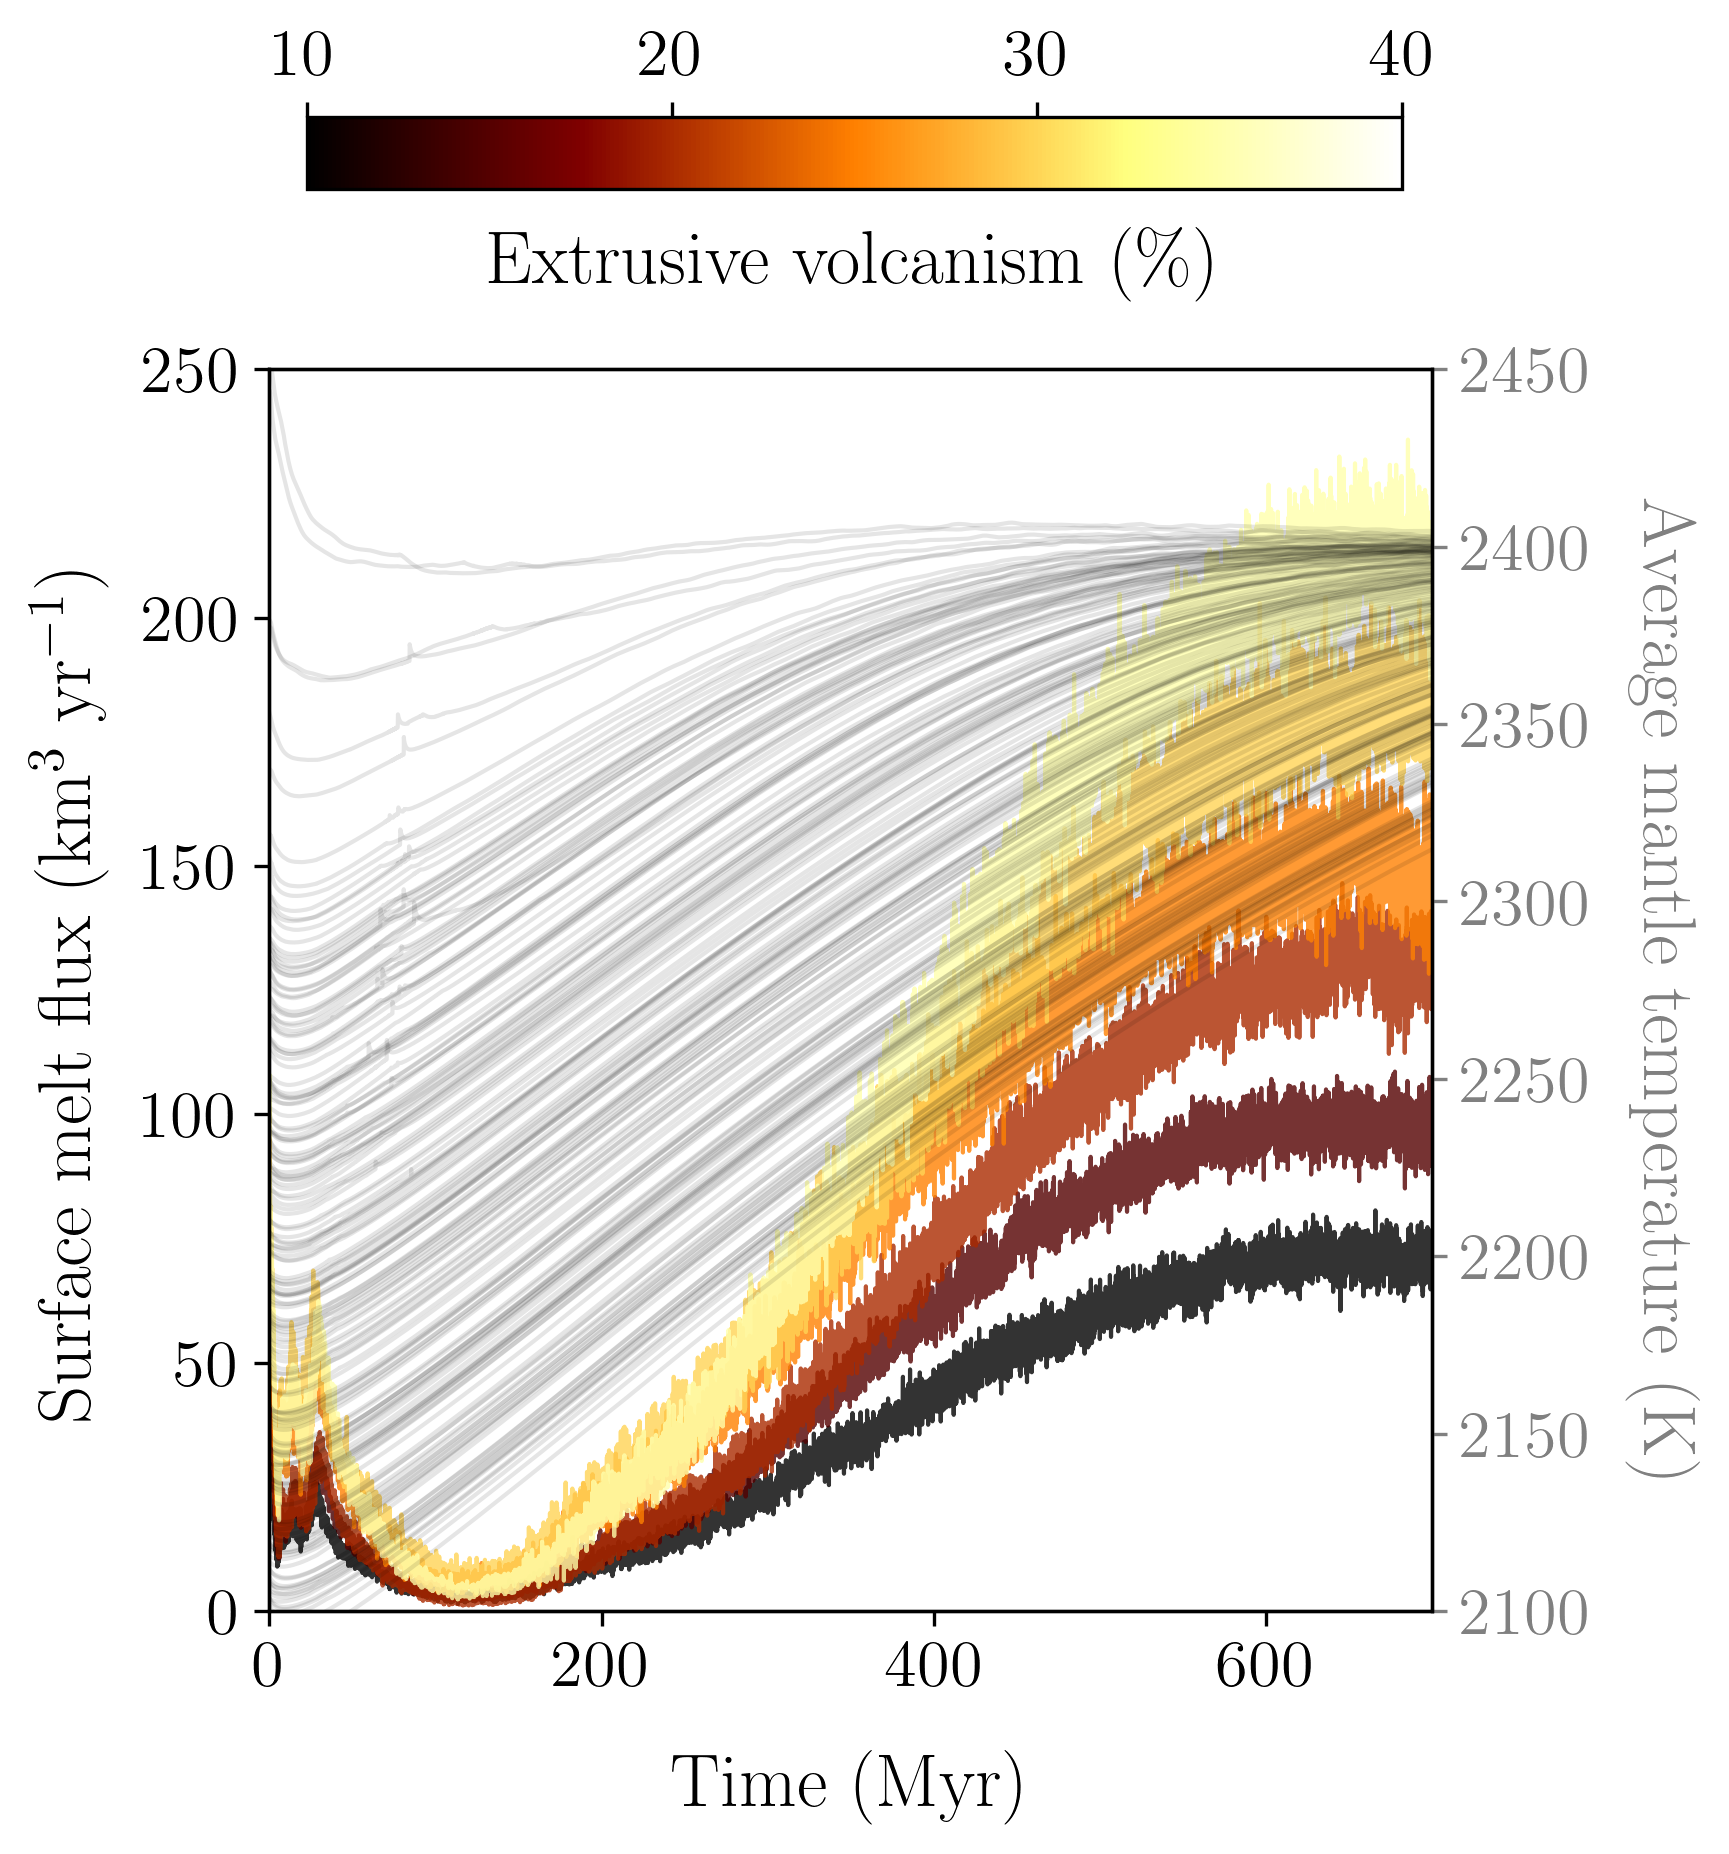
\includegraphics[width=0.7\linewidth]{melt_evol.png}
    \caption[Modelled evolution of the extrusive volumetric melt production rate for Archean Earth.]{The evolution of the extrusive volumetric melt production rate, assuming a melt density of 3000~kg~m$^{-3}$. Note that these values represent only 10--40\% of the total melt production. Cases are binned to 5\%-increments in the extrusive volcanism fraction, and averaged over all other input parameters (Table \ref{tab:inputs}). Lighter colours indicate higher extrusive volcanism fractions. Overlain in solid grey lines and corresponding to the secondary $y$-axis are the evolutions of the mean temperature over the whole mantle, for each individual model run.}
    \label{fig:melt_vol}
\end{figure}

\subsubsection{Choice of extrusive volcanism percentages}

Only a fraction of melt will rise high enough to extrude and outgas at the surface, which we refer to as the extrusive volcanism percentage. The remaining melt will be emplaced; we assume it will eventually replenish the mantle. \citet{Crisp1984} estimate an extrusive volcanism percentage of 6--25\% for intracontinental and island arc settings, and 16--33\% at mid-ocean ridges and hotspots. Because this value is unknown for early Earth, we allow it to vary between 10\% and 40\% \citep{Grott2011}. We do not consider any diffuse degassing from intrusive magmatism, although fluid pressure would indeed transport intrusive magmatic gas to the surface through rock fissures.  






\section{Results}

Before speciation, the total C (or H) outgassing flux is proportional to the product of the C (or H) melt concentration and the extrusive melt production rate. In principle, either of these factors has the potential to scale outgassing dramatically, although they do not necessarily show the same variance. We will first present the melt production rates and melt concentrations from the model. Then we will describe the resulting outgassing fluxes, their final speciation modulated by $f_{\ch{O2}}$.


\subsection{Thermal history and melt production}




The thermal histories underlying the outgassing model are shown in Fig. \ref{fig:melt_vol}. Mean mantle temperatures gradually increase due to powerful primordial radiogenic heating and relatively sluggish stagnant lid convection. The temperature dependence of viscosity acts as a thermostat, such that by 700~Myr, average mantle temperatures converge to $\sim$2320--2400~K.

The first $\sim$50~Myr see spikes in the melt flux---the magnitude of which depends on $T_{\rm ini}$---followed by a decrease and subsequent settling to a steady value. Directly after magma ocean solidification, the mantle temperature is still very close to the solidus. In these conditions, slight mass movement from convection can trigger immediate re-melting. This depletes the residual mantle and raises the solidus temperature. Melting is revived once either radiogenic heating warms the upper mantle, or convection upwells undepleted material from the lower mantle to pressures of $\le$12~GPa. 


Note that higher initial temperatures than considered here would lead to unphysical conditions, with most of the mantle above the solidus temperature. Whilst a much wetter mantle might aid melting, we do not find a dramatic effect of $\chi_{\ch{H2O}}^{\rm ini}$ on the overall melt production. We do not include dehydration's stiffening effect on viscosity.


\subsection{Melt contents of \ch{H2O} and \ch{CO2}}


\begin{figure}%
    \centering
    \subfloat{{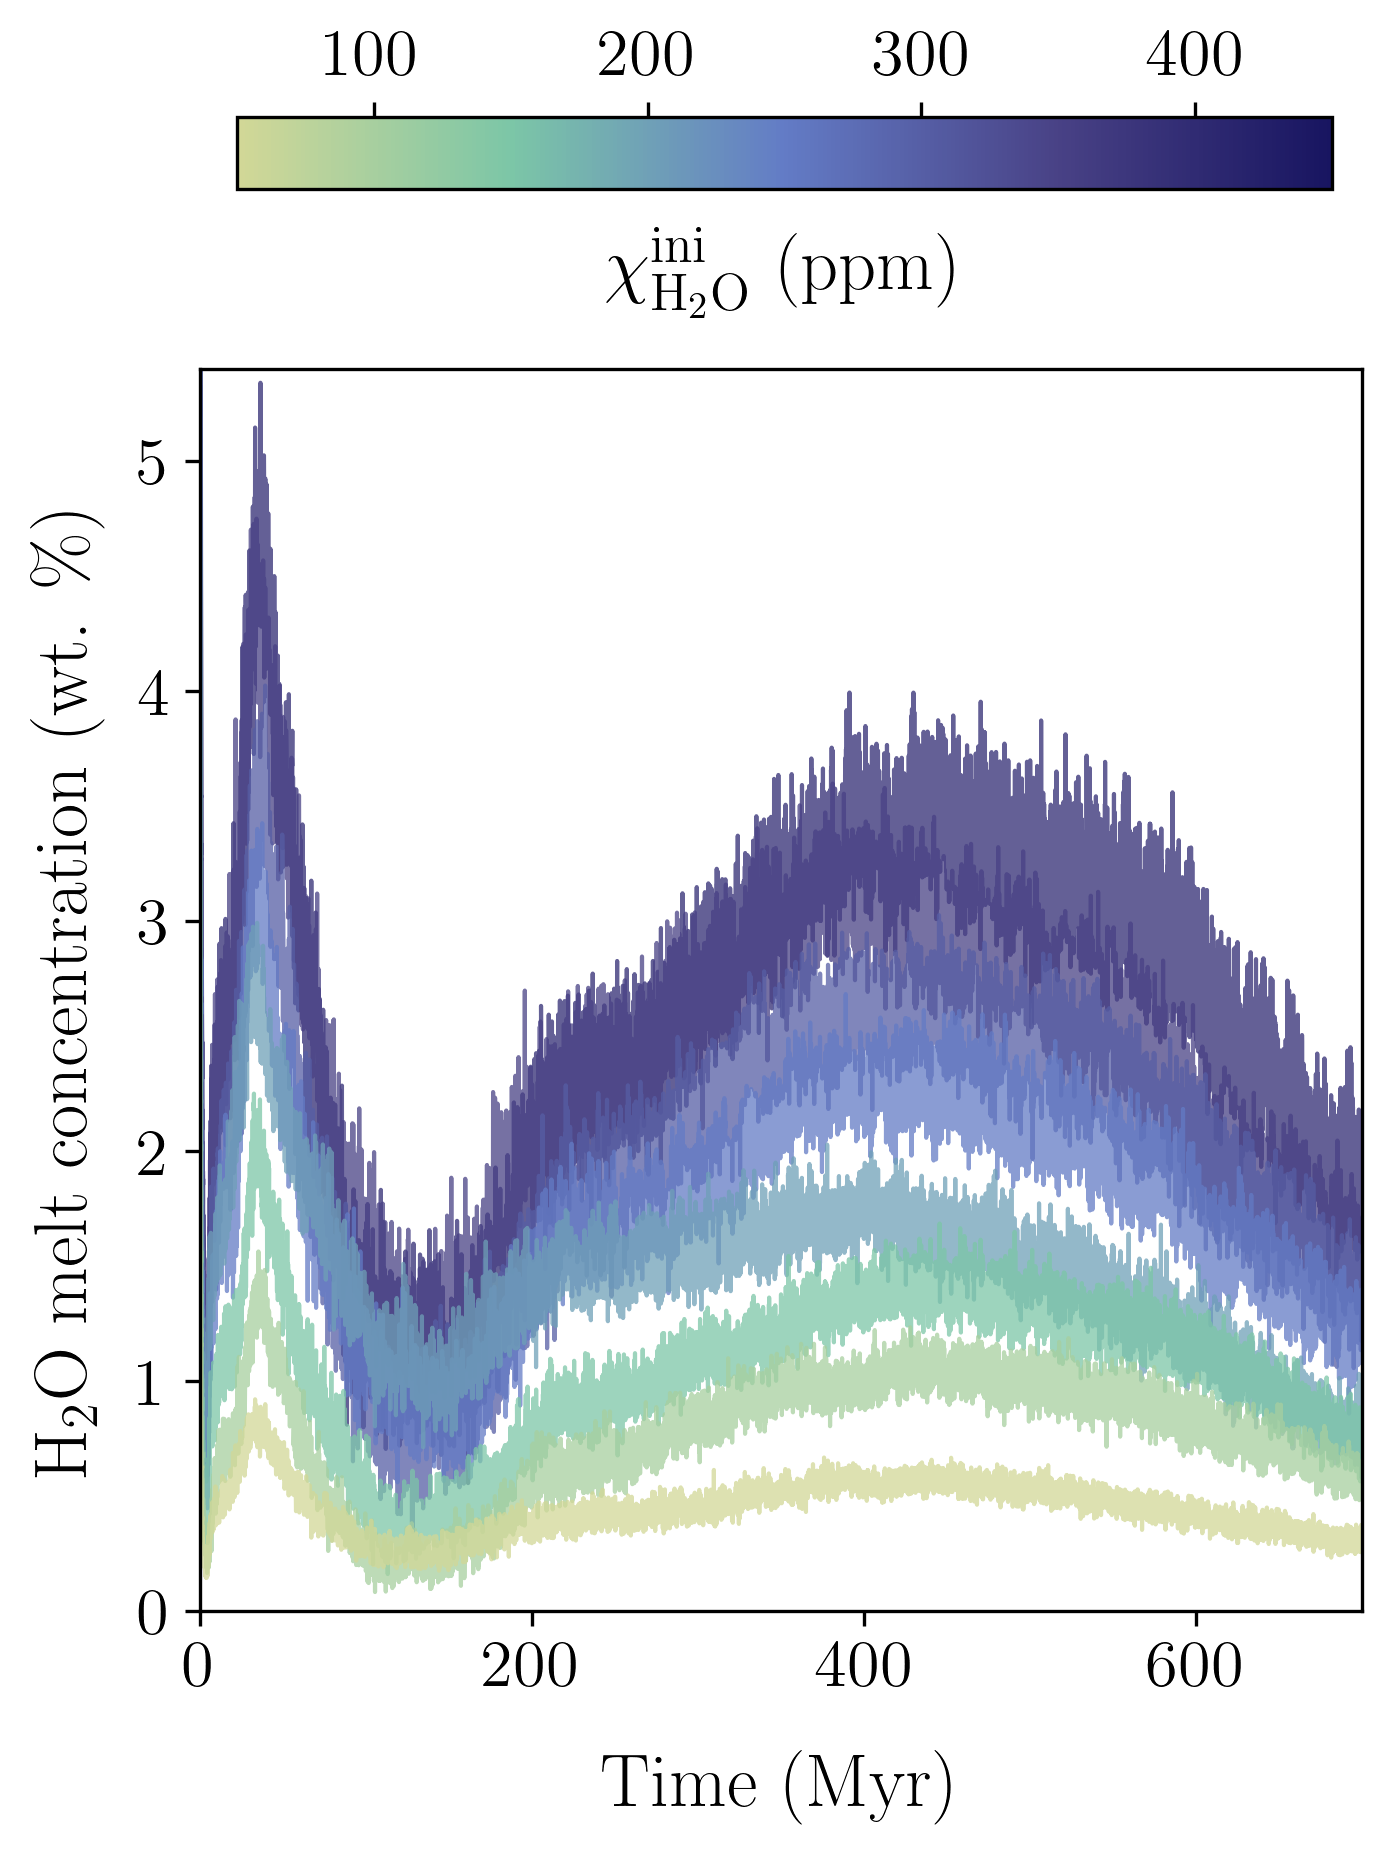
\includegraphics[width=0.45\linewidth]{XH2O_evol.png} }}%
    \qquad
    \subfloat{{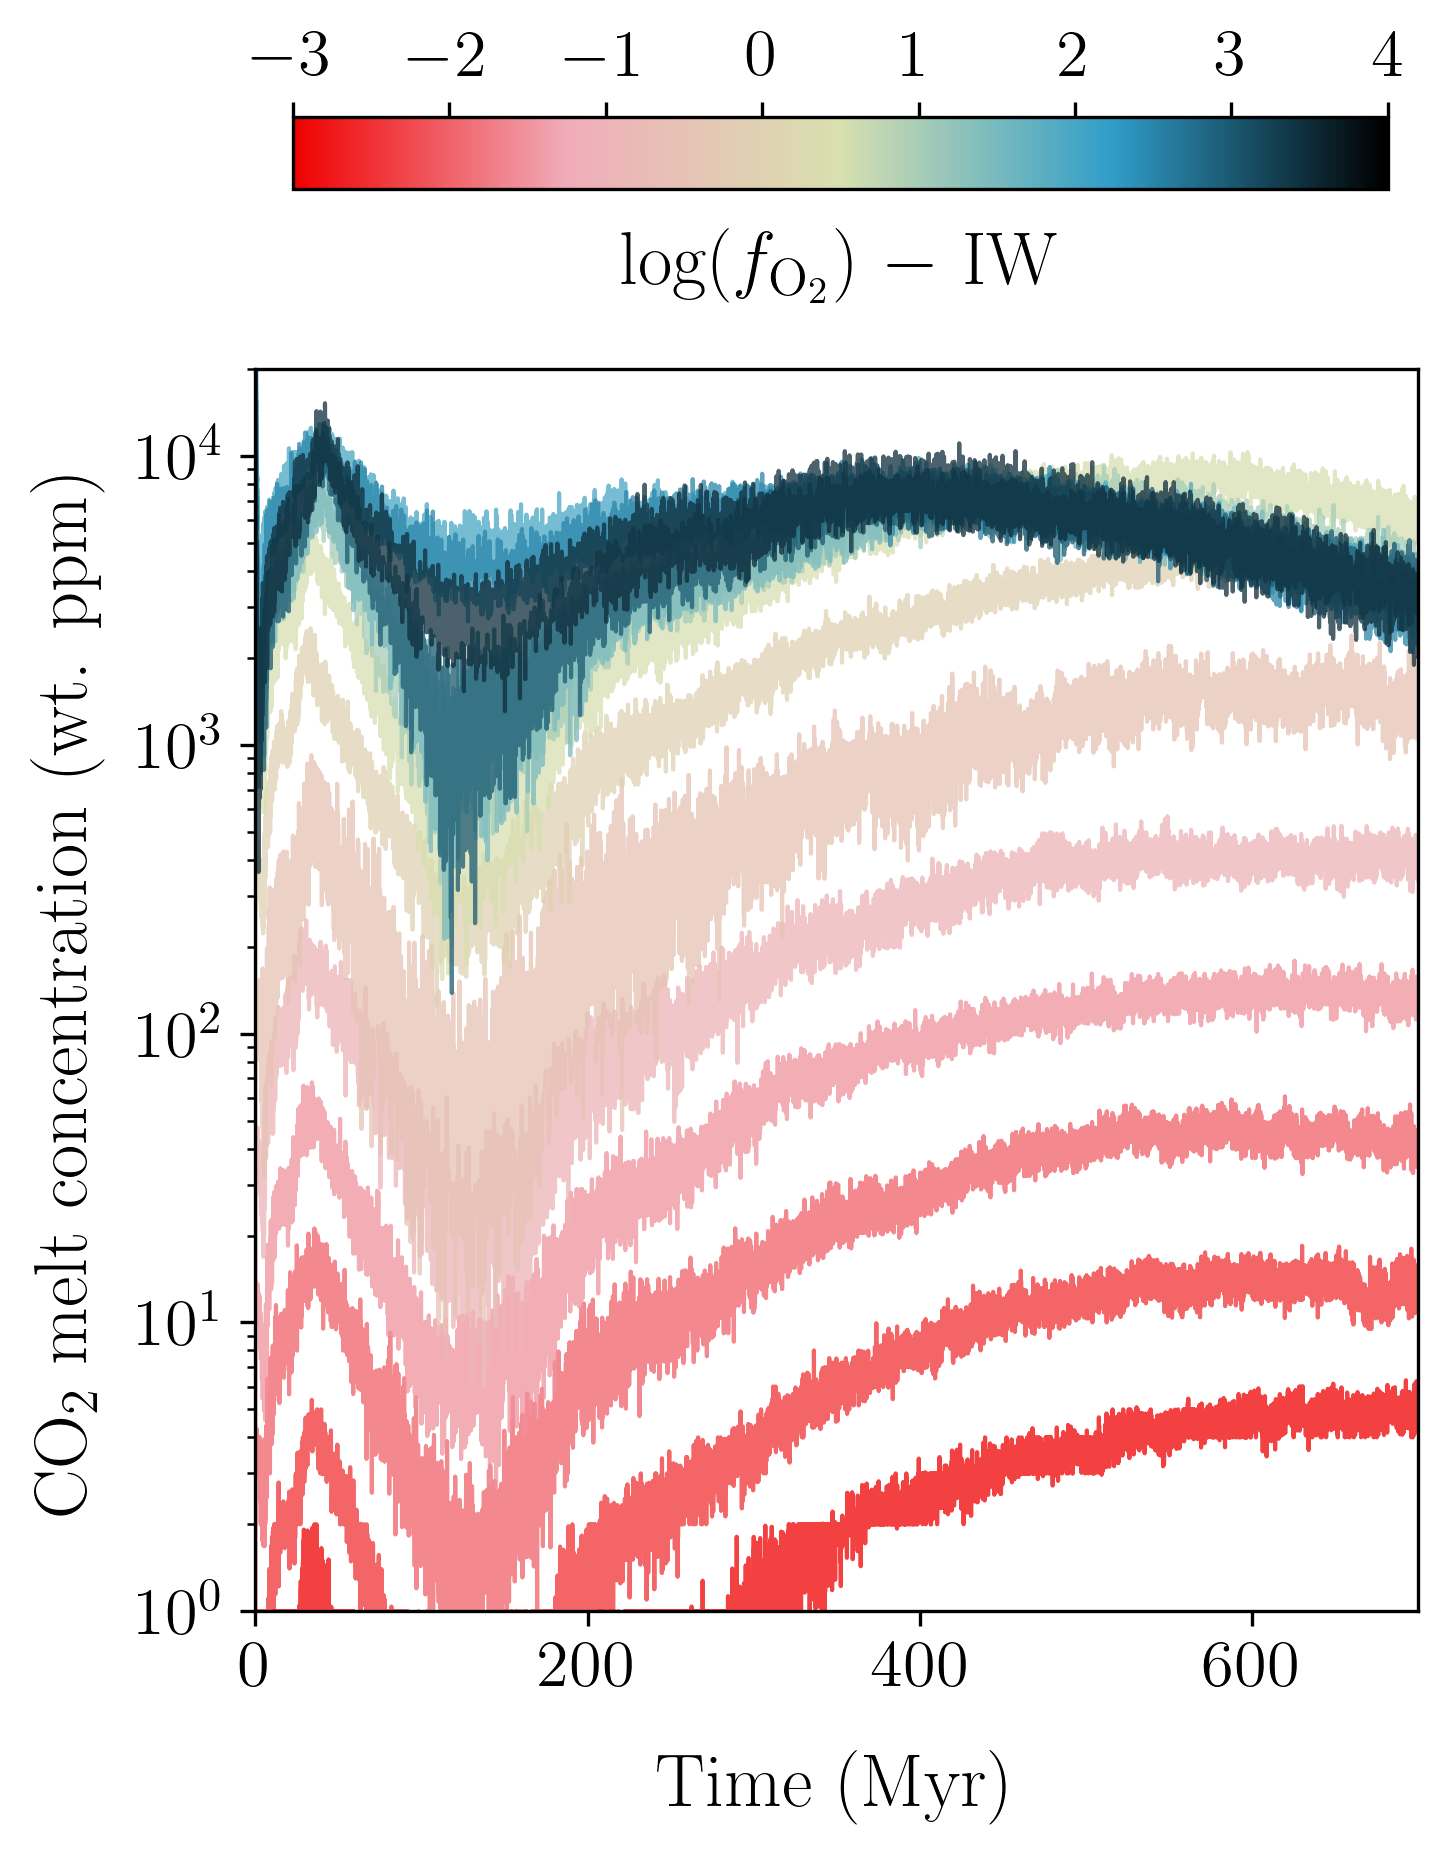
\includegraphics[width=0.465\linewidth]{XCO2_evol.png} }}%
    \caption[Modelled evolution of melt volatile contents for \ch{H2O} and \ch{CO2} for Archean Earth.]{The evolution of melt volatile contents for \ch{H2O} (\textit{left}; in weight percent) and \ch{CO2} (\textit{right}; in weight ppm). Cases are binned according to their values of the main input parameter controlling melt partitioning (see text): for \ch{H2O} this is the initial mantle \ch{H2O} content ($\chi_{\ch{H2O}}^{\rm{ini}}$), and for \ch{CO2} this is the mantle oxygen fugacity ($f_{\ch{O2}}$) with respect to the iron-w\"ustite buffer (IW). Lines are coloured by bin and show the mean melt concentration per time interval, given random values for the other input parameters.}%
    \label{fig:X_melt}%
\end{figure}






Due to the different chemistry controlling the partitioning of C and \ch{H2O} into the melt (section \ref{sec:partitioning-methods}), $\chi_{\ch{H2O}}^{\rm melt}$ and $\chi_{\ch{CO2}}^{\rm melt}$ respond to different model parameters. These behaviours are reflected in Fig. \ref{fig:X_melt}. \ch{H2O} partitioning into the melt depends directly on the local mantle \ch{H2O} abundance, the maximum of which is set by $\chi_{\ch{H2O}}^{\rm ini}$. The effect of mantle content on melt content is non-linear: in equation (\ref{eq:h_partition}), $\chi_{\ch{H2O}}^{\rm melt}$ depends on the local melt fraction, whilst the presence of water facilitates melting by suppressing the solidus.


Carbon partitioning, in contrast, is strongly redox-dependent. This is true for the regime we model, where graphite is the stable phase, but would not apply to more oxidising conditions \citep{Stagno2019}. Note, that the local mantle source \ch{CO2} concentration can still limit $\chi_{\ch{CO2}}^{\rm melt}$. This effect is most obvious at very low values of $\chi_{\ch{CO2}}^{\rm ini}$ below 50~ppm, or for cases approaching maximum outgassing---in either situation the local carbon inventories can run out. The most carbon-rich simulations can be seen (Fig. \ref{fig:X_melt}) to reach peak $\chi_{\ch{CO2}}^{\rm melt}$ before 700 Myr for this reason. Meanwhile, the effect of $f_{\ch{O2}}$ on $\chi_{\ch{CO2}}^{\rm melt}$ is drastic everywhere. With each step of one log-unit below the IW buffer, we see $\chi_{\ch{CO2}}^{\rm melt}$ drop by an order of magnitude.

There is an early transient stage where the melt abundance drops steeply. This is associated with the early pulse of melting and hence depletion (Fig. \ref{fig:melt_vol}). 

\subsection{Exploration of outgassing scenarios}



A notable result of this work is that all scenarios, regardless of oxidation state, produce outgassing no higher than total estimates for modern Earth \citep[e.g.,][]{Catling2017}. To see why this is, here we examine what controls outgassing rates in this model.

\subsubsection{Outgassing as a function of mantle oxidation state}


\begin{figure}
    \centering
    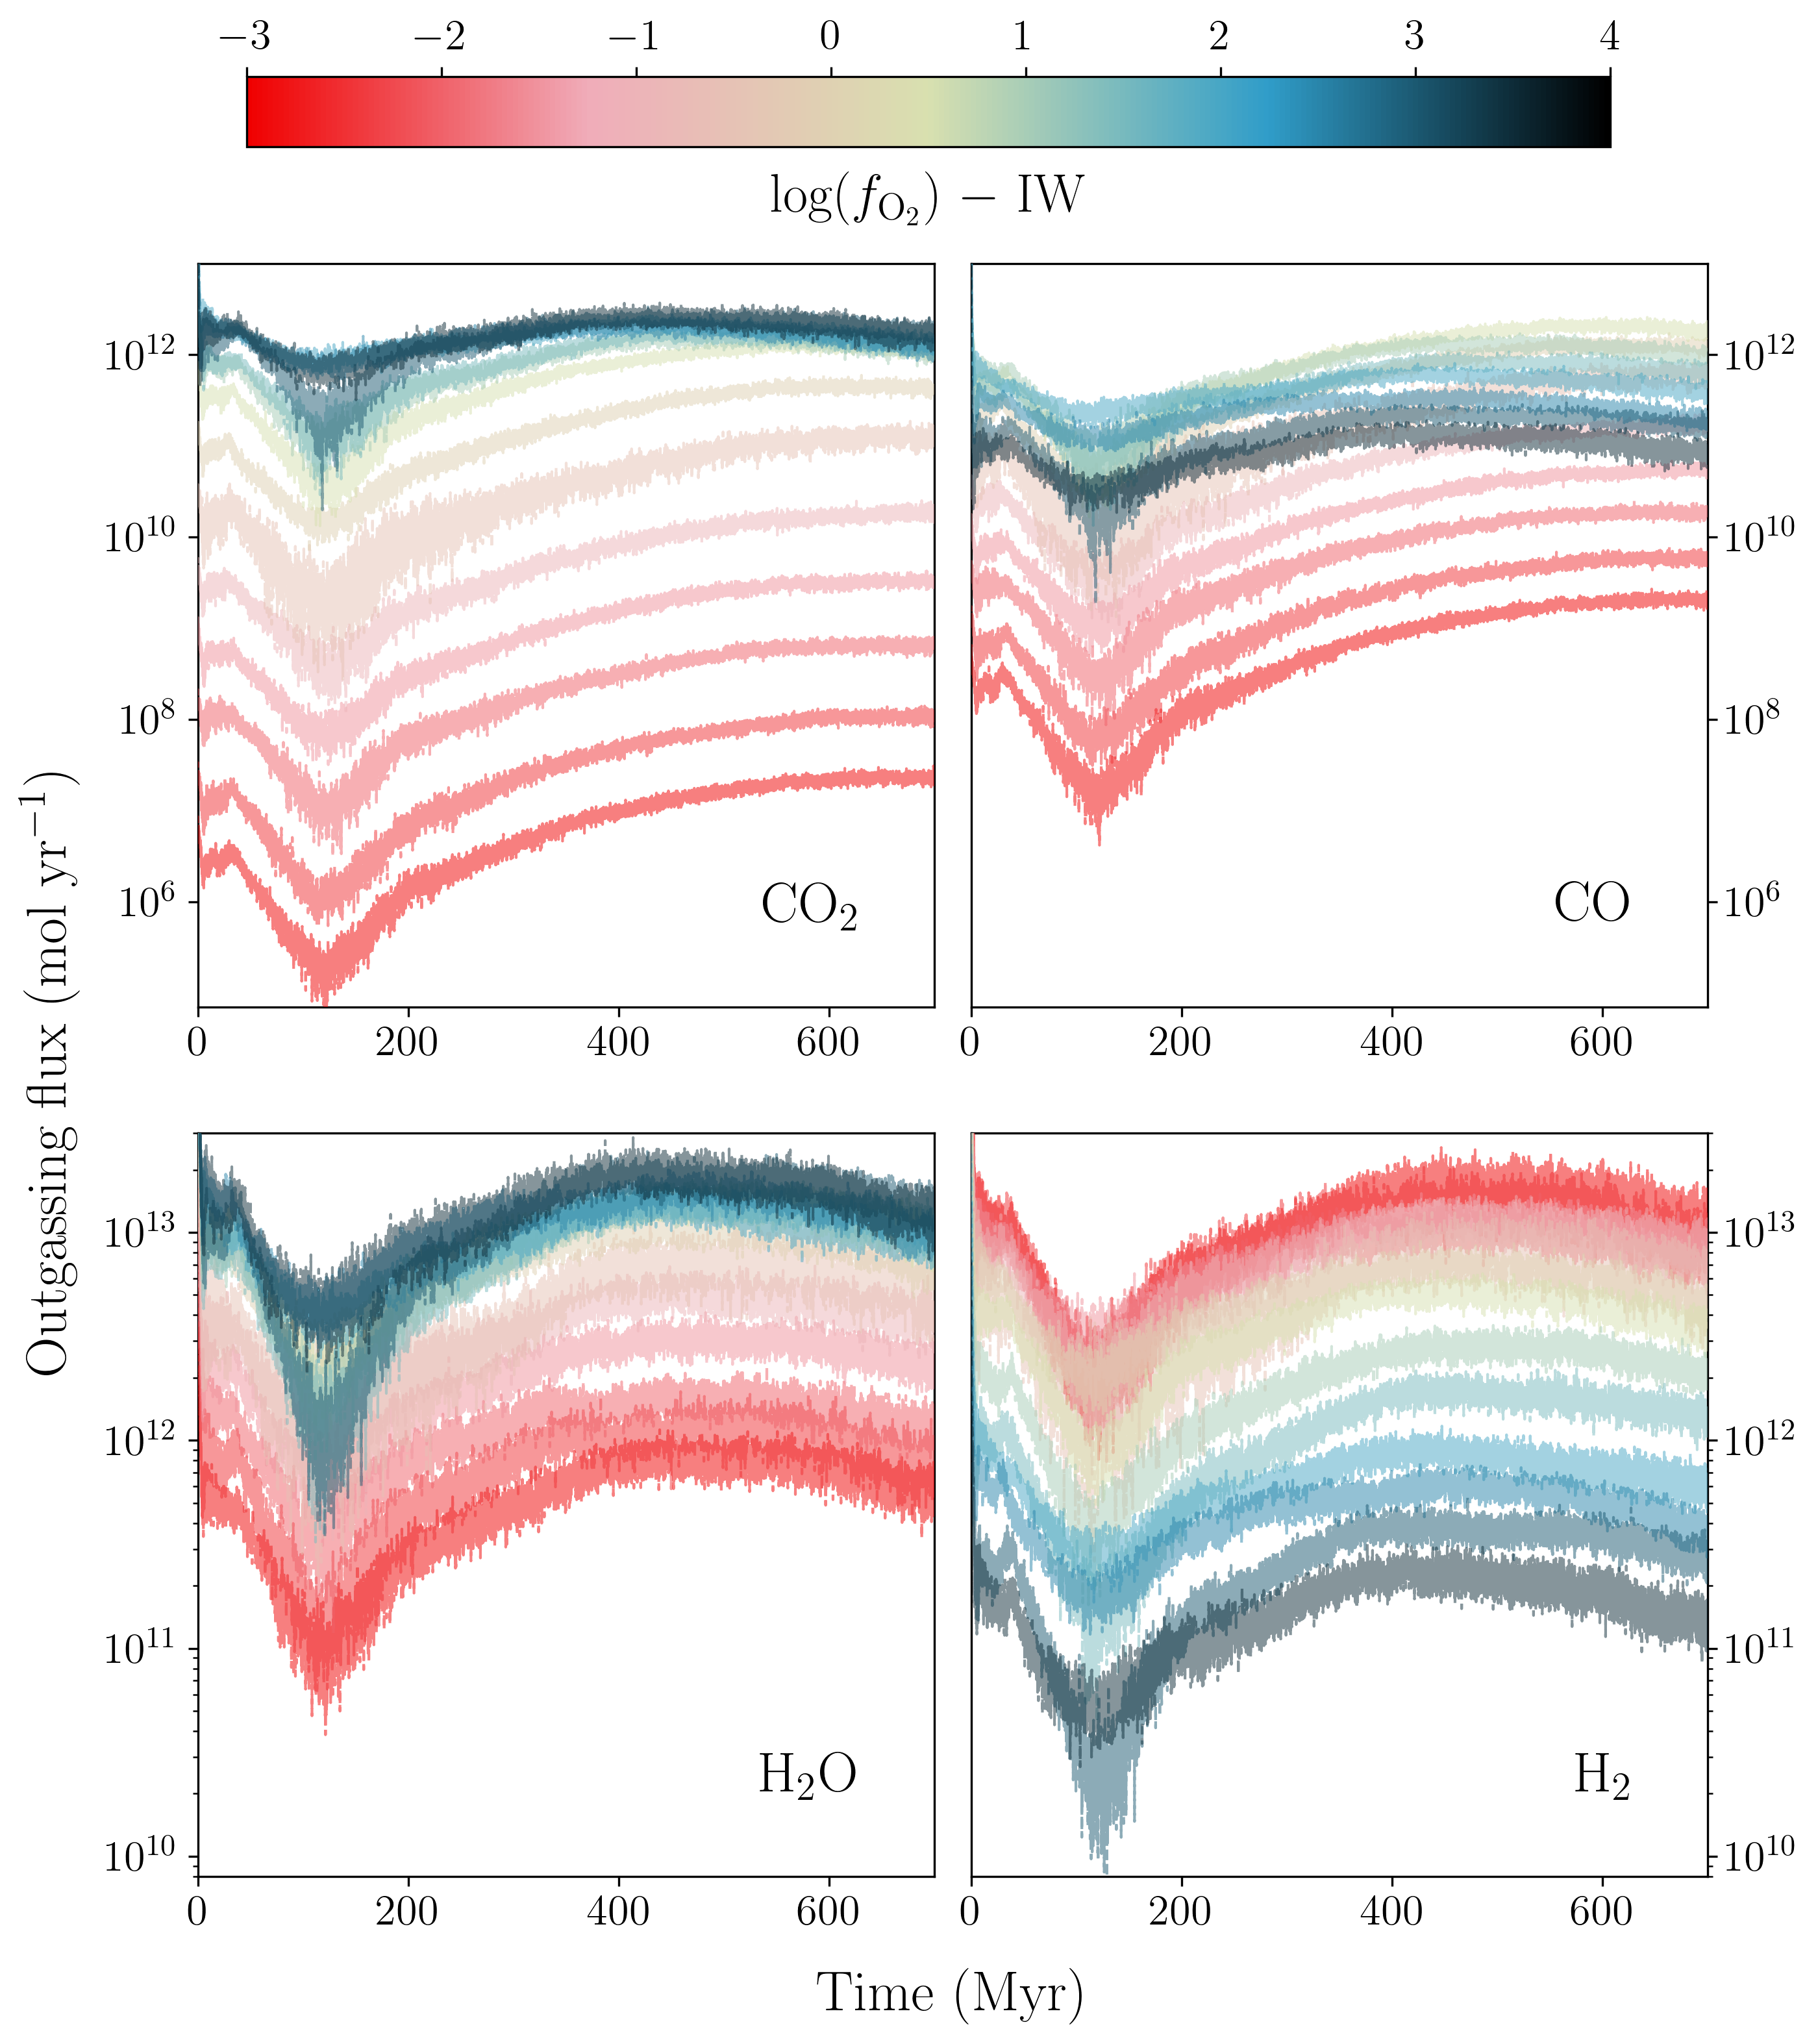
\includegraphics[width=1\linewidth]{flux_evol.png}
    \caption[Modelled evolution of outgassing fluxes of \ch{CO2}, \ch{CO}, \ch{H2O}, and \ch{H2} for Archean Earth.]{The mean evolution of volcanic outgassing fluxes for \ch{CO2} \textit{(top left)}, \ch{CO} \textit{(top right)}, \ch{H2O} \textit{(bottom left)}, and \ch{H2} \textit{(bottom right)}. Coloured lines from red to dark blue indicate increasingly oxidised mantles, binned to increments of 0.5 log-units in mantle oxygen fugacity ($f_{\ch{O2}}$) with respect to the iron-w\"ustite buffer (IW), and averaged across all other input parameters. }
    \label{fig:fO2_flux}
\end{figure}

\begin{figure}
    \centering
    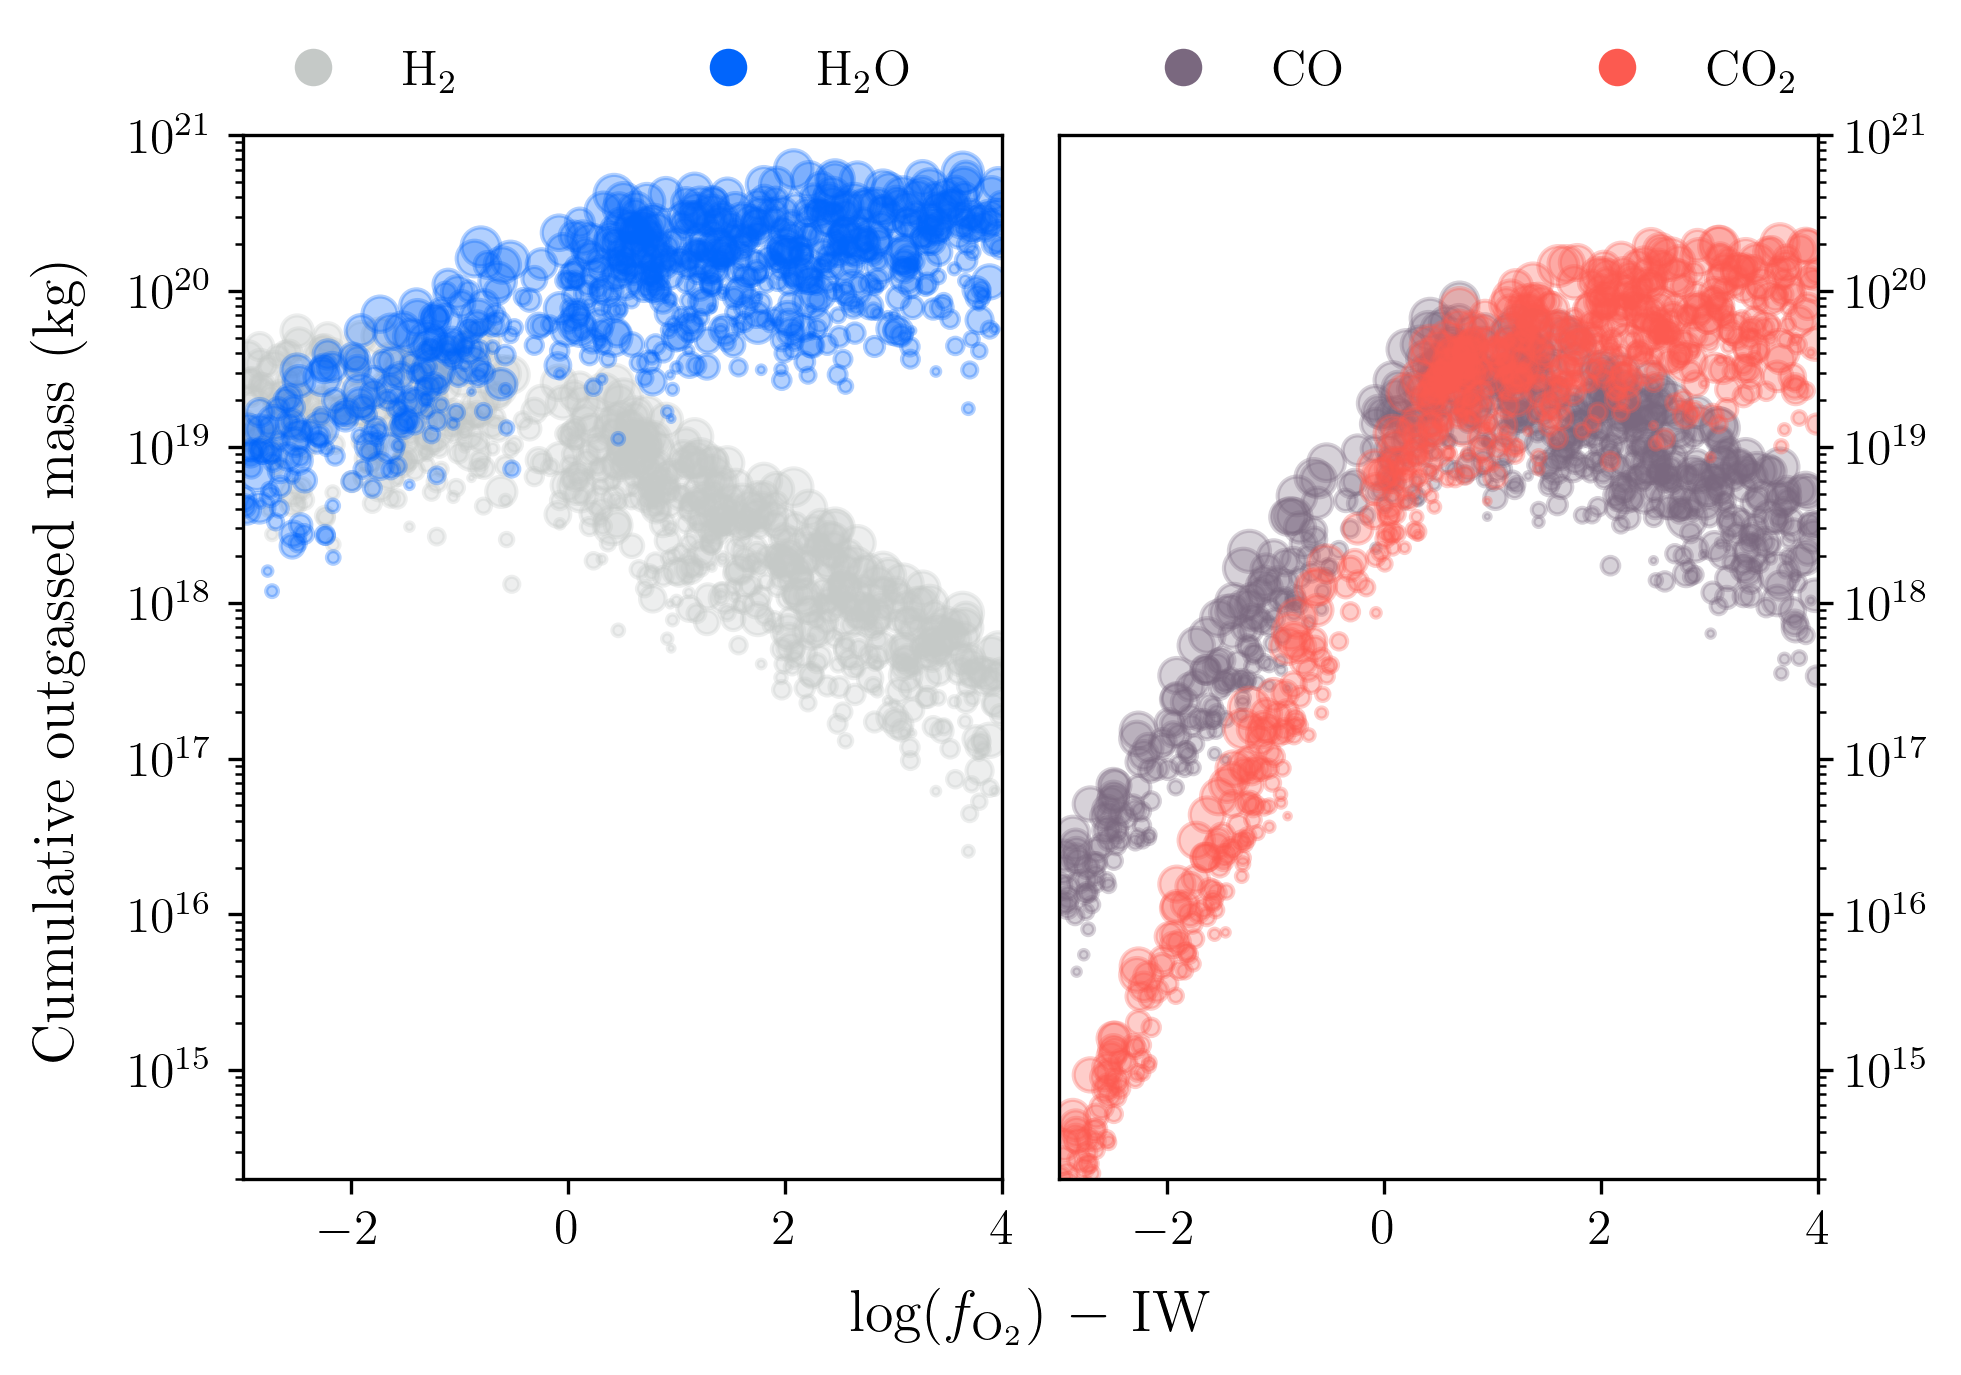
\includegraphics[width=1\linewidth]{masses_scatter.png}
    \caption[Total cumulative outgassed masses of \ch{H2}, \ch{H2O}, \ch{CO}, and \ch{CO2}, as a function of \fo.]{Each simulation's final cumulative outgassed masses of \ch{H2} (grey dots), \ch{H2O} (blue dots), \ch{CO} (aubergine dots), and \ch{CO2} (coral dots), as a function of the mantle oxygen fugacity ($f_{\ch{O2}}$) with respect to the iron-w\"ustite buffer (IW). Marker size increases with higher cumulative melt volume. All \Ncases~parameter combinations are shown.}
    \label{fig:fO2_scatter}
\end{figure}

As expected \citep{Holland1984, kasting_mantle_1993}, there is a heavy dependence of the outgassing rate on $f_{\ch{O2}}$. Fig. \ref{fig:fO2_flux} shows the evolution of each species' mean outgassing flux in mol yr$^{-1}$, with cases binned by $f_{\ch{O2}}$ and all other input parameters varying according to a random uniform distribution (Table \ref{tab:inputs}). A more oxidised mantle is associated with more \ch{CO2} and \ch{H2O} outgassing, and a more reduced mantle is associated with more \ch{H2} outgassing. The pattern for \ch{CO} is more complicated. It peaks around IW: low $f_{\ch{O2}}$ limits the amount of total carbonate that can dissolve into the melt, despite the gas-phase equilibrium favouring \ch{CO} over \ch{CO2}. Outgassing rates increase slightly with time (by 10--15\%) during the 700 Myr modelled. The early pulse of outgassing is associated with the early pulse of melting (Fig. \ref{fig:melt_vol}). 





To illustrate the dependence of evolved outgassing on $f_{\ch{O2}}$, Fig. \ref{fig:fO2_scatter} shows every run's cumulative outgassed mass per species, as a function $f_{\ch{O2}}$. Both C- and H-bearing species are well-separated in terms of mass, except for cases close to the IW buffer. Increasing $f_{\ch{O2}}$ from IW~$-$~3 to IW~$+$~4 is associated with an increase of over an order of magnitude in the mass of \ch{H2O}, and an increase of at least five orders of magnitude for \ch{CO2}, whilst the mass of \ch{H2} decreases. The hydrogen speciation shows a gradient in redox. The carbon speciation also shows a gradient in redox, whilst the total amount of carbon depends on partitioning (itself a function of redox).

It is worth emphasising that Fig. \ref{fig:fO2_scatter} does not show the actual gas masses residing in the atmosphere. For instance, the atmospheric partial pressure of \ch{H2O} is limited to the saturation vapour pressure of liquid water; on the Myr-timescales of this model, the cooling timescale of the outgassed plume to ambient atmospheric temperatures is irrelevant. At $T_{\rm surf} = 333$~K, the saturation vapour pressure is 0.2~bar. The cumulative mass of \ch{H2O} (which would quickly condense) is at most about a tenth of modern Earth's ocean mass, which would support the idea that earlier magma ocean degassing supplied a significant fraction of the original ocean mass \citep{Pahlevan2019}.

The influence of $f_{\ch{O2}}$ on the outgassed volatile masses is built into the model. Intrinsically, there are three reasons for the mass dependence in Fig. \ref{fig:fO2_scatter}. The first two reasons comprise the redox-dependent speciation (setting total carbon) and volatile speciation (setting [\ch{H2O}]/[\ch{H2}] and [\ch{CO2}]/[\ch{CO]}) already described. The third reason is that the reduced gases investigated here have a lower molecular mass than their oxidised counterparts. Thus, for equal quantities outgassed, reduced atmospheres are necessarily less massive than oxidised atmospheres. 




\subsubsection{Other factors influencing outgassing}








Fig. \ref{fig:corr} summarises the Spearman's rank (nonlinear) correlation coefficients between each species' outgassing flux, averaged over the final 10 Myr, and the eight input parameters plus the melt volumes and volatile concentrations. This section explains how the remaining correlations stem from the model.

\paragraph{Influence of initial temperatures}

We find virtually no correlation between initial temperature conditions and outgassing fluxes after 700~Myr of convection. However, an initially hotter mantle closer to the solidus temperature forces a sharp pulse of melting in the first 100 Myr, expelling massive amounts of water and indeed raising the total mass of water outgassed. This is also not to say that instantaneous local temperatures are unimportant, as they affect the melt fraction as well as the equilibrium constants in (\ref{eq:c_partition}), (\ref{eq:equilibrium_constant_hydrogen}), and (\ref{eq:equilibrium_constant_carbon}).




\paragraph{Influence of extrusive volcanism fractions}

From (\ref{eq:m_atm}), we expect an approximately linear relationship between the maximum outgassing flux and the fraction of melt allowed to contribute to outgassing. Although the correlation between this fraction and the computed outgassing fluxes is not as strong as $f_{\ch{O2}}$, accounting for extrusive volcanism in this model automatically downscales outgassing. For example, all else being equal, the difference between $\chi_{\rm extr}=10$\% and $\chi_{\rm extr}=100$\% would be an order of magnitude in outgassing.


\paragraph{Role of melt production rate versus melt volatile content}

Fig. \ref{fig:corr} also shows the correlations of all outgassing fluxes with the instantaneous volatile melt concentrations and melt production rates. \ch{CO2} outgassing fluxes correlate more strongly with \ch{CO2} melt concentrations than with the total melt production rates, whilst the opposite appears to be true for \ch{H2O}. Note that \ch{H2O} melt concentrations are not independent of melt volumes because of partitioning of water into the melt---\ch{H2O} concentrations are largest for the smallest melt fractions. To some degree, the relative strengths of the correlations reflect the experimental variances in melt production and volatile melt contents, given the ranges of the prior distributions on the input parameters. Nevertheless, in our simulations, outgassing will be ultimately limited by the volatile budget of the mantle. Thus rates of outgassing would not scale indefinitely with rates of volcanism.

\begin{figure}
\centering
  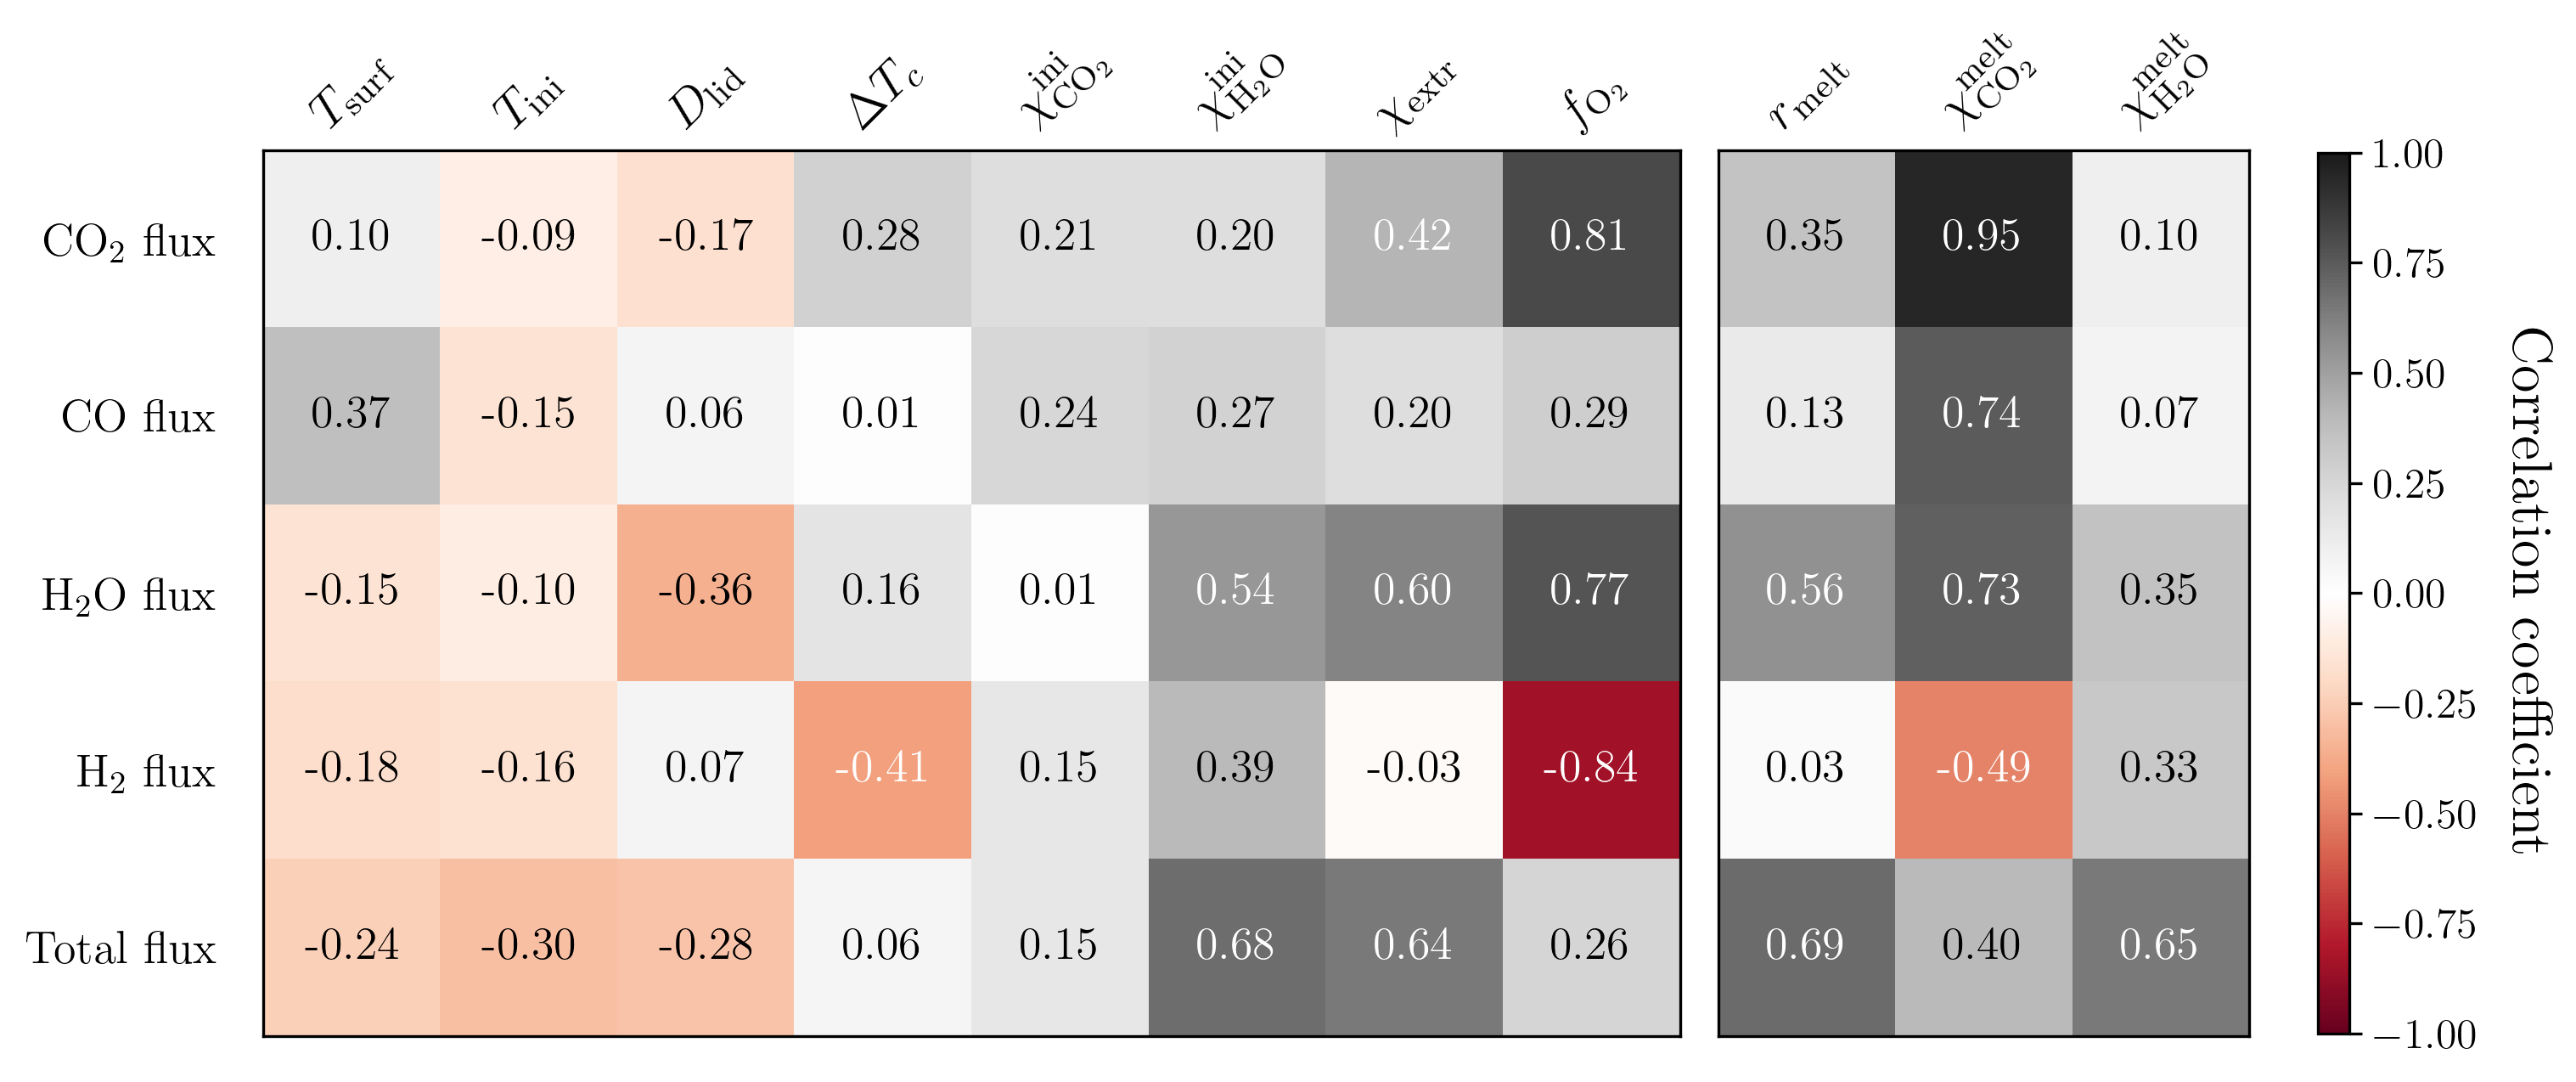
\includegraphics[width=\linewidth]{corr.png}
\caption[Matrix of correlation coefficients between key parameters and outgassing fluxes.]{\textit{(Left:)} The matrix of Spearman's rank correlation coefficients between input parameters and outgassing fluxes averaged over the final 10~Myr, plus the summed flux of all outgassed molecules for the same time frame. Symbols are defined in Table \ref{tab:inputs}. \textit{(Right:)} The same, but for key intermediate output variables---the volumetric melt production rate, $r_{\rm melt}$, and the melt concentrations of \ch{CO2} and \ch{H2O}, $\chi_{\ch{CO2}}^{\rm melt}$ and $\chi_{\ch{H2O}}^{\rm melt}$. Note that the moderate correlation between $\chi_{\ch{CO2}}^{\rm melt}$ and H-species outgassing is due to the mutual effect of $f_{\ch{O2}}$ on both quantities, while the correlation of $f_{\ch{O2}}$ with the total flux appears low because it does not affect the sum of \ch{H2} and \ch{H2O}.}\label{fig:corr}
\end{figure}



\subsubsection{Redox-marginalised outgassing distributions}



Fig. \ref{fig:hist_mass_fo2} presents the experimental distributions of each species' cumulative outgassed partial pressures, shown for different redox bins. Again, the dominant effect of $f_{\ch{O2}}$ is visible in how these distributions are separated along the $x$-axis. The median and 1$\sigma$ values of these partial pressures are quantified in Table \ref{tab:results}, along with the corresponding masses and fluxes.  



\begin{figure}
\centering
  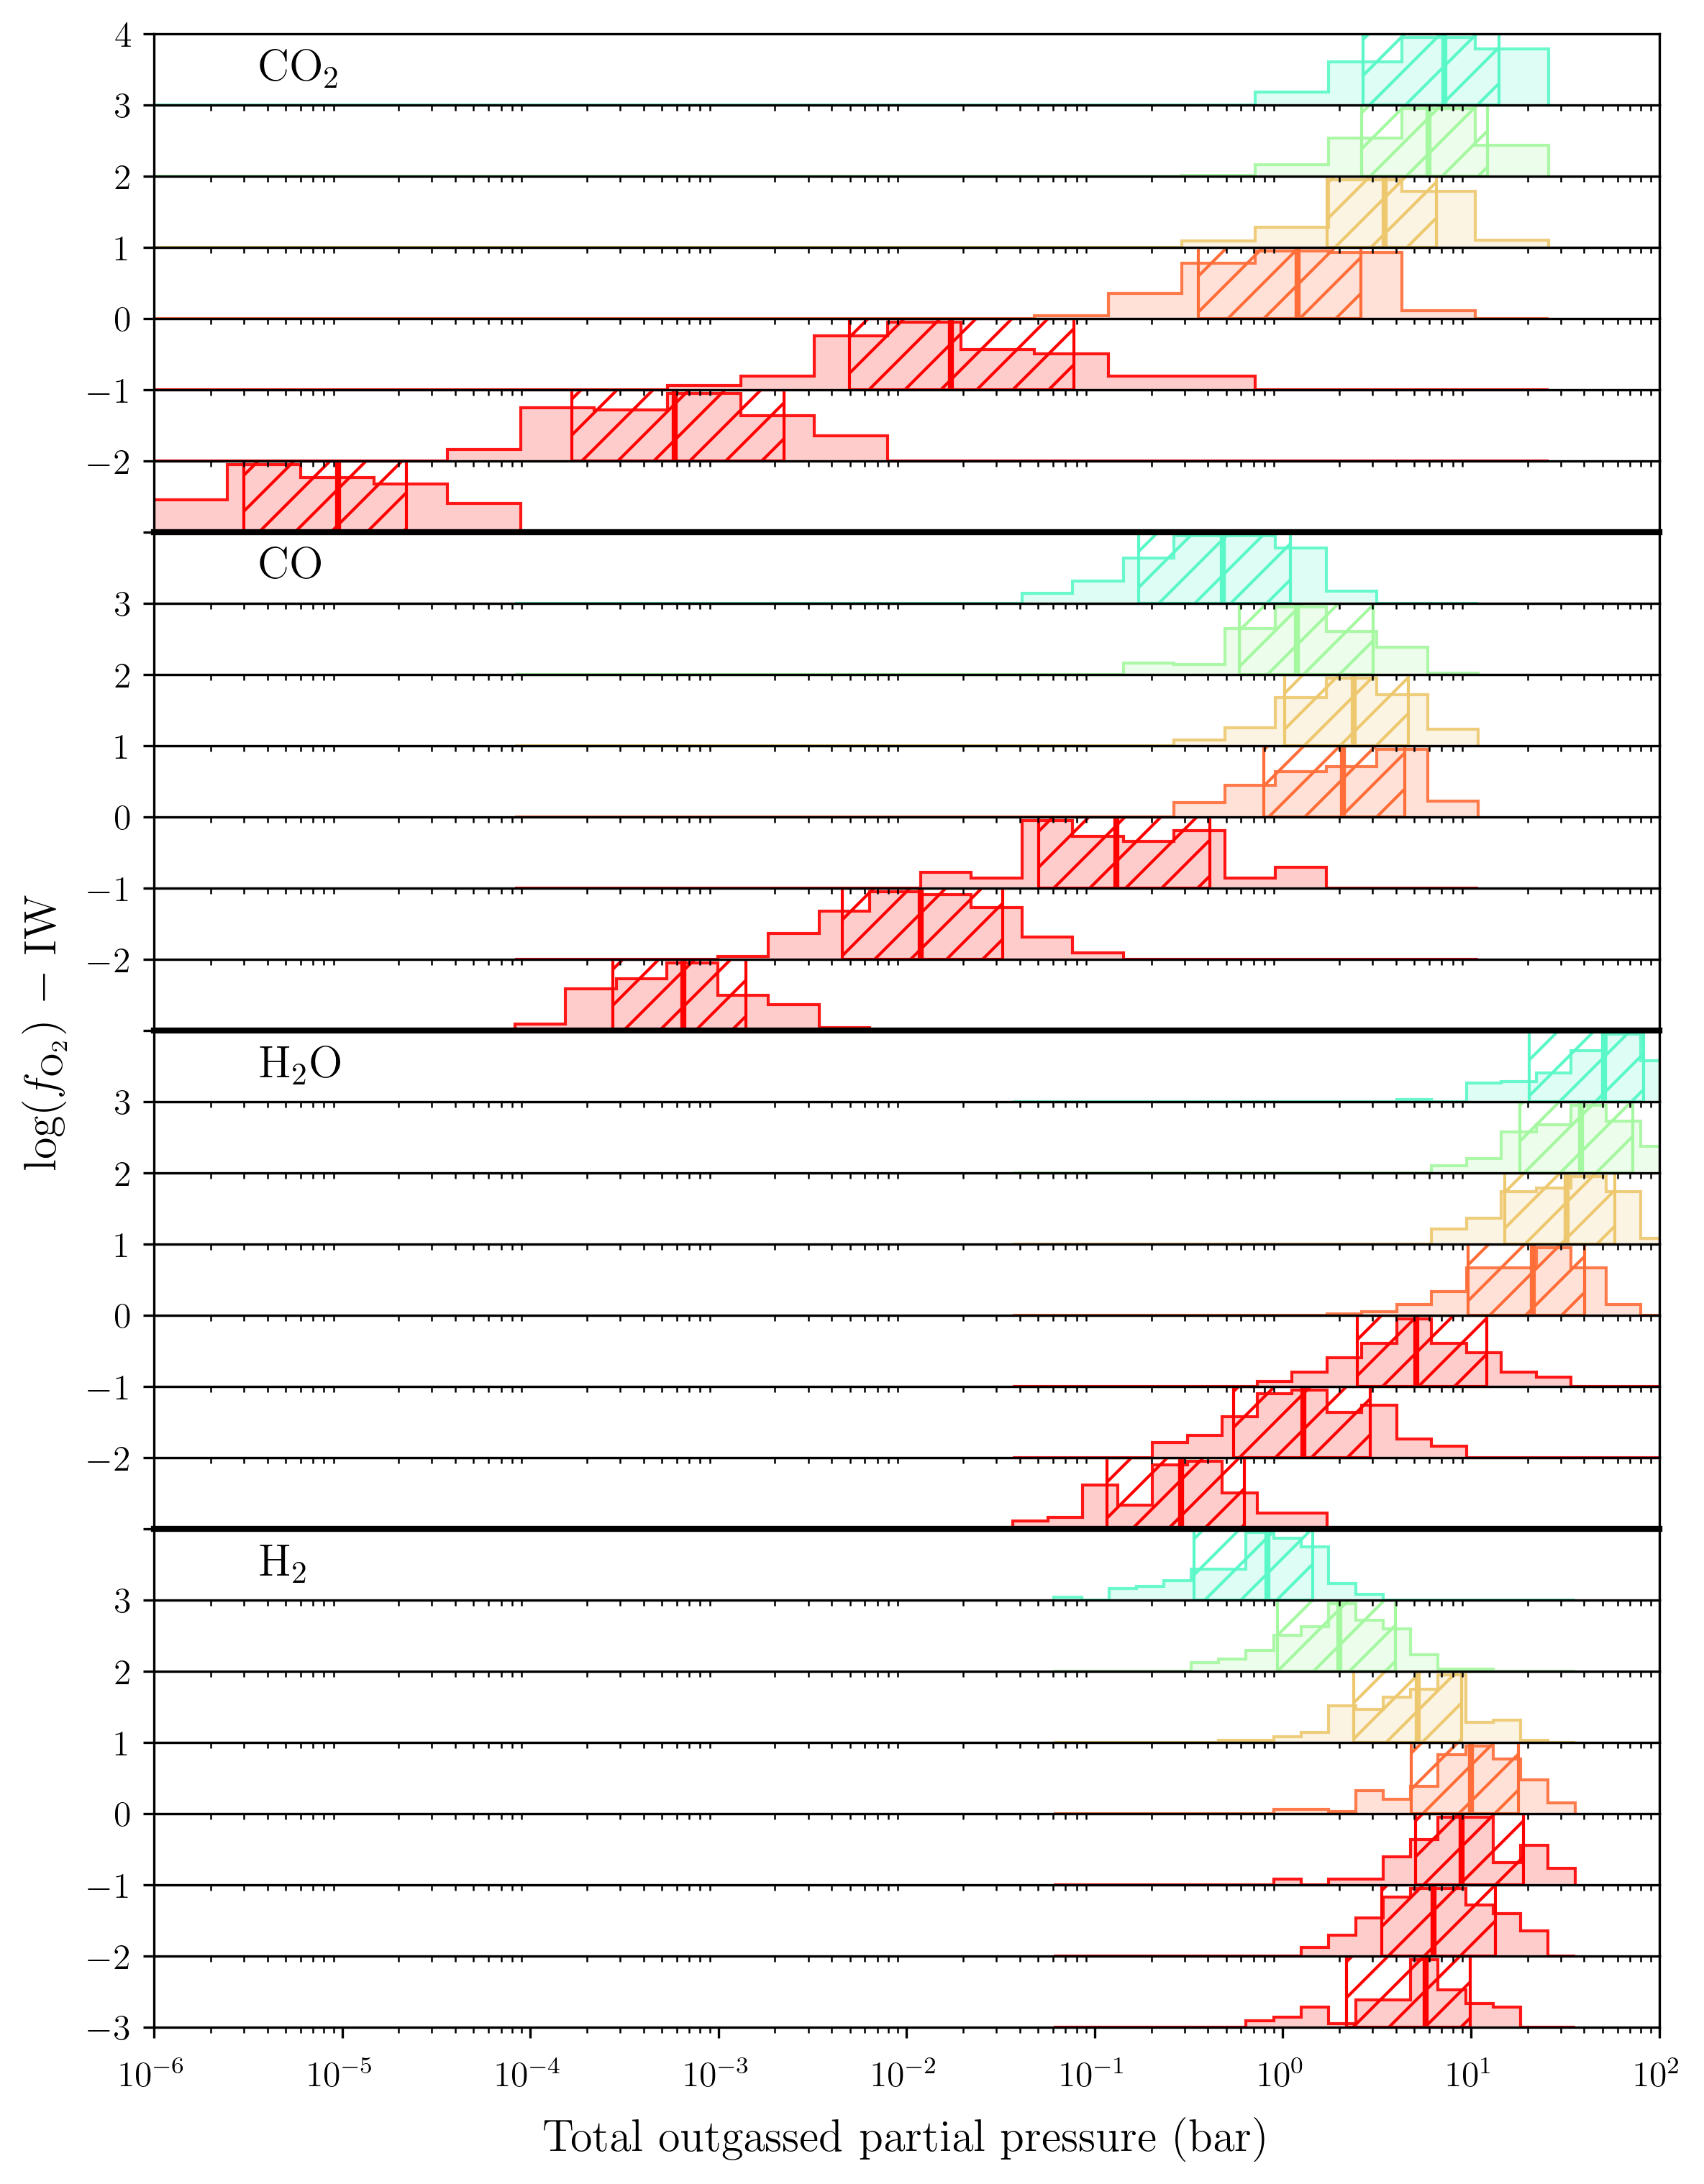
\includegraphics[width=0.9\linewidth]{hist_pressure.png}
\caption[Distributions of cumulative outgassed masses of \ch{CO2}, \ch{CO}, \ch{H2O}, and \ch{H2}, over uniformly-random draws of unknown input parameters.]{The distributions of 700-Myr-cumulative outgassed masses of (from top to bottom) \ch{CO2}, \ch{CO}, \ch{H2O}, and \ch{H2}, over \Ncases~draws of unknown input parameters from uniform distributions (Table \ref{tab:inputs}). Distributions are marginalised across the mantle oxygen fugacity ($f_{\ch{O2}}$) with respect to the iron-w\"ustite buffer (IW), where each colour shows one of five log($f_{\ch{O2}}$) bins as indicated by the $y$-axis ticks. Bold vertical lines indicate the medians; hatched regions mark the 1$\sigma$ width.\label{fig:hist_mass_fo2}}
\end{figure}




\begin{table*}
% \footnotesize
%\def\arraystretch{1.8} 
\caption[Outgassed partial pressures, masses, and fluxes of \ch{CO2}, \ch{CO}, \ch{H2O}, and \ch{H2} estimated for a stagnant lid Archean Earth.]{Final partial pressures, masses, and fluxes for each species after 700~Myr of outgassing, binned by mantle oxygen fugacity ($f_{\ch{O2}}$) with respect to the iron-w\"ustite buffer (IW). Fluxes represent averages over the last 10~Myr. Results are shown as the bin medians, with 1$\sigma$ limits super- and subscripted.}       
\label{tab:results}     
\begin{adjustbox}{width=1\textwidth}
\centering
\footnotesize                         

% paste below from python

\begin{tabular}{>{\centering\arraybackslash}m{3cm} l p{0mm} *{7}{r}}
\toprule
\noalign{\vskip 1mm}
 & & & \multicolumn{7}{c}{log($f_{\mathrm{O}_2}$) $-$ IW} \\
\cmidrule(lr){4 - 10}
& & & [-3, -2)& [-2, -1)& [-1, 0)& [0, 1)& [1, 2)& [2, 3)& [3, 4] \\
\noalign{\vskip 1mm} \midrule \noalign{\vskip 1mm}
Final pressure
 & 
CO$_2$ & 
& $0.0_{-0.0}^{+0.0}$
& $0.0_{-0.0}^{+0.0}$
& $0.0_{-0.0}^{+0.1}$
& $1.2_{-0.8}^{+1.4}$
& $3.5_{-1.8}^{+3.1}$
& $5.9_{-3.3}^{+6.3}$
& $7.2_{-4.5}^{+6.8}$
\\
(bar)
 & 
CO & 
& $0.0_{-0.0}^{+0.0}$
& $0.0_{-0.0}^{+0.0}$
& $0.1_{-0.1}^{+0.3}$
& $2.1_{-1.3}^{+2.3}$
& $2.4_{-1.4}^{+2.3}$
& $1.2_{-0.6}^{+1.8}$
& $0.5_{-0.3}^{+0.6}$
\\
 & 
H$_2$O & 
& $0.3_{-0.2}^{+0.3}$
& $1.3_{-0.7}^{+1.6}$
& $5.1_{-2.7}^{+7.0}$
& $21.3_{-11.7}^{+18.7}$
& $32.2_{-17.0}^{+26.2}$
& $38.5_{-20.3}^{+34.0}$
& $51.0_{-30.6}^{+31.4}$
\\
 & 
H$_2$ & 
& $5.7_{-3.5}^{+4.2}$
& $6.4_{-3.0}^{+7.1}$
& $8.9_{-3.8}^{+10.0}$
& $10.0_{-5.2}^{+7.9}$
& $5.2_{-2.8}^{+3.7}$
& $2.0_{-1.1}^{+2.0}$
& $0.8_{-0.5}^{+0.6}$
\\
\noalign{\vskip 1mm} \midrule \noalign{\vskip 1mm}
Final mass
 & 
CO$_2$ & 
& $0.0_{-0.0}^{+0.0}$
& $0.0_{-0.0}^{+0.1}$
& $0.5_{-0.3}^{+1.3}$
& $15.3_{-9.6}^{+19.0}$
& $40.7_{-21.5}^{+30.2}$
& $59.6_{-29.9}^{+52.0}$
& $66.7_{-38.2}^{+72.1}$
\\
(kg $\times 10^{18}$)
 & 
CO & 
& $0.0_{-0.0}^{+0.0}$
& $0.3_{-0.2}^{+0.5}$
& $2.2_{-1.2}^{+3.9}$
& $19.0_{-10.9}^{+20.6}$
& $16.1_{-8.3}^{+15.7}$
& $7.5_{-3.5}^{+10.0}$
& $3.1_{-1.9}^{+3.8}$
\\
 & 
H$_2$O & 
& $9.4_{-5.5}^{+7.8}$
& $23.9_{-11.9}^{+27.1}$
& $57.9_{-27.1}^{+60.4}$
& $128.7_{-74.1}^{+106.6}$
& $154.9_{-93.6}^{+129.0}$
& $171.7_{-102.4}^{+153.2}$
& $220.2_{-142.1}^{+137.2}$
\\
 & 
H$_2$ & 
& $18.2_{-10.4}^{+18.2}$
& $13.3_{-6.2}^{+14.3}$
& $12.2_{-6.2}^{+10.5}$
& $6.8_{-3.7}^{+5.7}$
& $2.8_{-1.7}^{+2.3}$
& $1.0_{-0.6}^{+0.9}$
& $0.4_{-0.2}^{+0.3}$
\\
\noalign{\vskip 1mm} \midrule \noalign{\vskip 1mm}
Final flux
 & 
CO$_2$ & 
& $0.0_{-0.0}^{+0.0}$
& $0.0_{-0.0}^{+0.0}$
& $0.0_{-0.0}^{+0.1}$
& $0.7_{-0.4}^{+1.2}$
& $1.3_{-0.8}^{+1.4}$
& $1.4_{-0.8}^{+1.6}$
& $1.8_{-1.2}^{+2.3}$
\\
(mol yr$^{-1}$ $\times 10^{12}$)
 & 
CO & 
& $0.0_{-0.0}^{+0.0}$
& $0.0_{-0.0}^{+0.0}$
& $0.2_{-0.1}^{+0.4}$
& $1.5_{-0.8}^{+1.8}$
& $0.9_{-0.5}^{+1.1}$
& $0.3_{-0.2}^{+0.5}$
& $0.1_{-0.1}^{+0.2}$
\\
 & 
H$_2$O & 
& $0.8_{-0.6}^{+0.9}$
& $1.9_{-1.2}^{+1.8}$
& $4.6_{-2.6}^{+4.2}$
& $9.1_{-5.4}^{+8.6}$
& $11.4_{-6.5}^{+13.1}$
& $11.3_{-7.8}^{+10.7}$
& $14.3_{-7.4}^{+15.9}$
\\
 & 
H$_2$ & 
& $12.9_{-8.1}^{+15.0}$
& $8.7_{-4.8}^{+7.6}$
& $8.2_{-5.0}^{+7.4}$
& $4.3_{-2.6}^{+3.7}$
& $1.8_{-1.1}^{+2.4}$
& $0.5_{-0.3}^{+0.8}$
& $0.2_{-0.1}^{+0.3}$
\\
\noalign{\vskip 1mm}
\bottomrule
\end{tabular}



% end python

\end{adjustbox}
\end{table*}












\subsection{Secular mantle oxidation}


\begin{figure}
\centering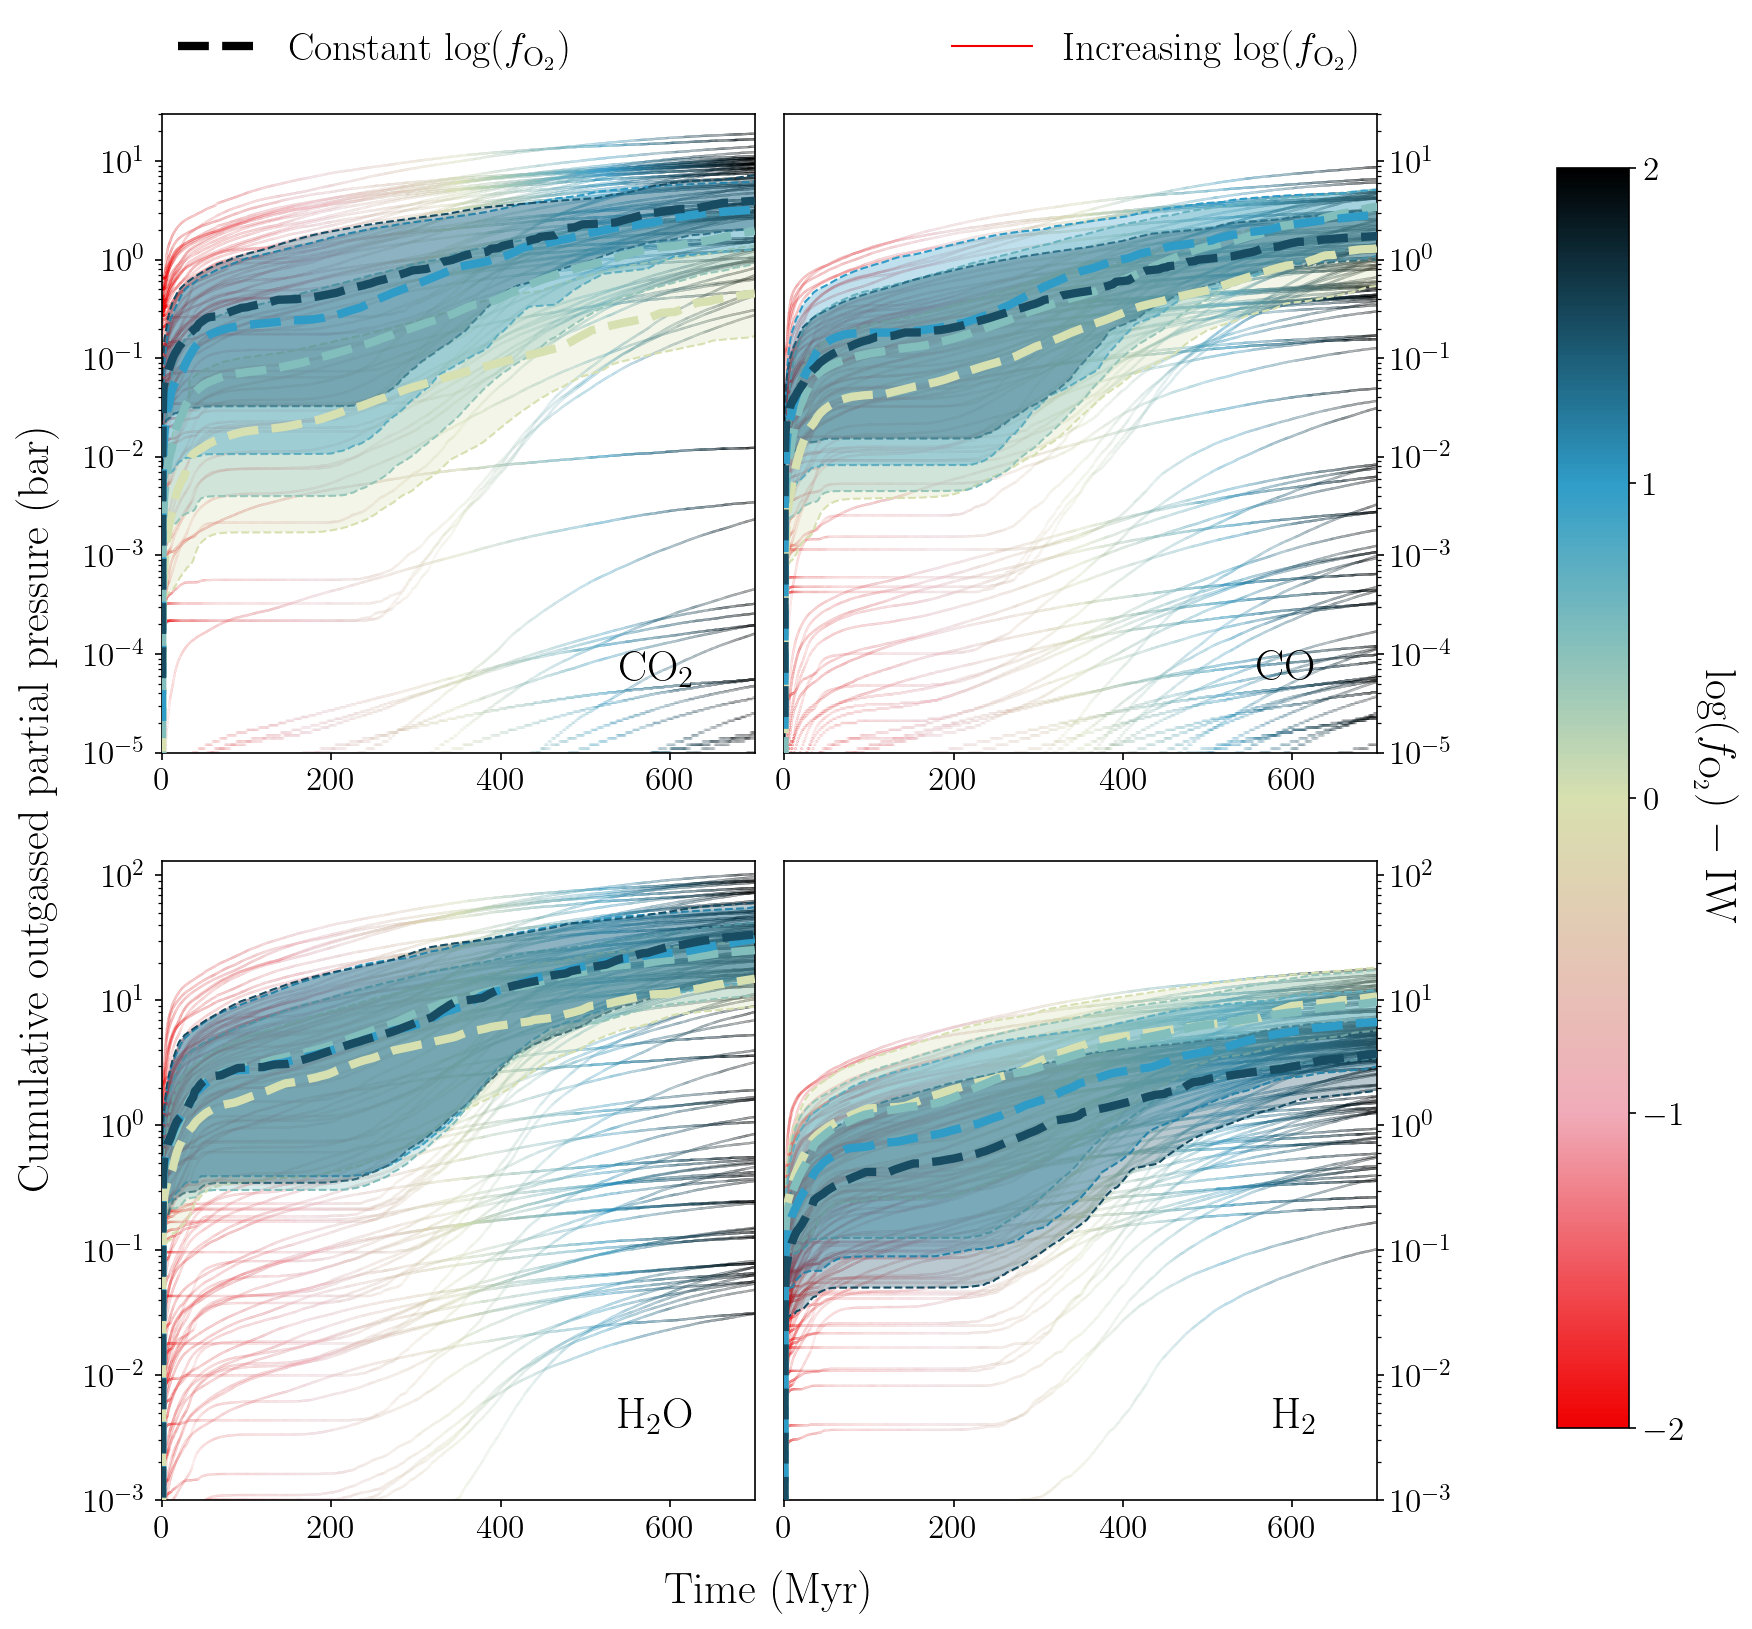
\includegraphics[width=1\linewidth]{pp_evol_fO2_increasing.png}
\caption[The evolution of cumulative outgassed partial pressures for scenarios where Archean Earth's mantle oxygen fugacity increases steadily over time.]{The evolution of the cumulative outgassed partial pressure for scenarios where the mantle oxygen fugacity ($f_{\ch{O2}}$) with respect to the iron-w\"ustite buffer (IW) increases log-linearly from IW~$-$~2 to IW~$+$~2 over 700~Myr (thin solid gradient lines; $N=110$). For comparison, also shown are the $f_{\ch{O2}}$-bin medians of previous scenarios where $f_{\ch{O2}}$ is fixed randomly between IW and IW~$+$~2 (thick dashed lines; $N=147$), where the thin dashed lines spanned by swaths indicate 1$\sigma$ above and below the median. Subplots show the species \ch{CO2} \textit{(top left)}, \ch{CO} \textit{(top right)}, \ch{H2O} \textit{(bottom left)}, and \ch{H2} \textit{(bottom right)}. The colour indicates the instantaneous mantle redox. \label{fig:evol_fo2increase}}
\end{figure}


Several mechanisms for mantle oxidation have been proposed \citep[e.g.,][]{Wood2006, sharp_hydrogenbased_2013, gaillard_theoretical_2014, wordsworth_redox_2018,  Schaefer2018, NICKLAS2019}, including degassing itself \citep{kasting_mantle_1993}. These mechanisms would be associated with different durations. By tracking the concentration of abundant multivalent cations, one might self-consistently evolve the mantle redox state within our outgassing scenarios. We leave this to future work, and as a first step, simply consider a linear increase of $\log (f_{\ch{O2}})$ from IW~$-$~2 to IW~$+$~2 over 700~Myr, for a new set of 110 runs with otherwise random parameters as before (Table \ref{tab:inputs}). 

Fig. \ref{fig:evol_fo2increase} demonstrates that secularly increasing $\log (f_{\ch{O2}})$ results in cumulative outgassing not obviously distinguishable from a constant $\log (f_{\ch{O2}}) - {\rm IW} \in [0, 2]$. The spread in these cases would be largely explained by variations in the melting rate.

Low $f_{\ch{O2}}$ does not affect melt concentrations of H-species, such that the same total amount of total H can be outgassed. Carbon, meanwhile, is strongly limited in melts during the early reduced stage, which might imply lower cumulative partial pressures. However, Fig. \ref{fig:evol_fo2increase} suggests that this effect is somewhat muted due to the scatter induced by other unknown parameters. Note, regardless, that small differences in cumulative outgassing could represent dramatic differences in the ultimate atmospheric composition; scenarios of evolving mantle redox likely deserve more rigorous treatment than attempted here.



%%%%%%%%%%%%%%%%%%%%%%%%%%%%%%%%%%%%%%


\section{Discussion}

\subsection{Some important considerations about the assumptions in this model}

\subsubsection{Viscosity treatment}

This work has considered a single set of upper mantle rheological parameters, corresponding to the canonical Arrhenius viscosity law for wet olivine from \citet{karato_rheology_1993}. Lower mantle rheology is taken from \citet{tackley_mantle_2013}.  Different viscosity treatments could potentially influence melting rates and therefore outgassing rates.

However, several regulation mechanisms exist such that an immediate weakening of upper mantle viscosity, whilst increasing the convective velocity, may not lead to dramatically higher melting in the long term. Firstly, latent heat loss associated with any melting that does occur would cool the mantle (the latent heat of melting is indeed modelled here). These lowered temperatures would both limit further melting and stiffen the local viscosity in a negative feedback loop \citep{Ogawa2011}. Secondly, a sudden increase in convective velocity would lead to faster replenishment of depleted material in the upper mantle, which promotes melting; yet, thirdly, this effect would be offset simultaneously by more efficient cooling of the mantle, which suppresses melting.

The \citet{karato_rheology_1993} law for wet diffusion creep does have a relatively weak temperature dependence and a strong pressure dependence, which could reduce some of the feedbacks described here. Nevertheless, as in \citet{dorn_outgassing_2018}, we expect that melting is ultimately controlled by the lower mantle viscosity because rapid flow in the upper mantle merely leads to rapid depletion. With that said, we would still emphasise that the results here are subject to our chosen viscosity treatment, and should be interpreted as such.


\subsubsection{Submarine versus subaerial outgassing}

We have assumed that all outgassing is subaerial and occurs at 1~bar. Several independent constraints place an upper limit on either the surface barometric pressure or $p\ch{N2}$ at 1.1~bar for 3.5--2.7~Ga \citep{Marty2013, Catling2020}. A lack of plate motion might allow volcanic eruptions to construct topography above sea level relatively quickly (e.g., Olympus Mons, a Martian shield volcano comparable to Germany in area). In this case, volatiles would degas freely from surface lavas at atmospheric pressure. Because near 1~bar there is almost no effect on gas solubility or $f_{\ch{O2}}$ in our chosen parameterisations, we do not consider solubility or any redox change during degassing itself. If most outgassing occurred on the seafloor, then the higher pressures would allow melts to retain more volatiles, as long as the gas and melt are in equilibrium (e.g., eruptions are not explosive). Global outgassing rates would then be lower than predicted here, and show a different ratio of outgassing species \citep{Gaillard2011}.


\subsubsection{Note on \ch{CH4} outgassing}

We neglect the outgassing of \ch{CH4} entirely because its vapour phase is not stable at the pressure, temperature, and redox ranges we consider \citep{zhang2009model, wetzel2013degassing, ramirez2014warming}. Some \ch{CH4} fluid could be produced from a reduced source at high pressures up to 11~GPa \citep{Scott2004}. Although \ch{CH4} can also be stable at surface pressures, melt temperatures would be too high for it to degas directly.


\subsubsection{Buoyancy limit of melting}

As in \citet{noack2014can, noack_volcanism_2017}, we have not considered the possibility of melting at depths greater than 12~GPa. This assumes that basaltic melt is not buoyant above this pressure because it is denser than olivine \citep{ohtani_melting_1995}. However, \citet{Mosenfelder2009} have suggested that basaltic melt can nevertheless remain less dense than ringwoodite and wadsleite up to $\sim$25 GPa. Therefore the actual density crossover pressure could be lower than modelled here \citep[e.g.,][]{Beuchert2013}. This could increase the volume of the mantle annulus in which melting can occur, possibly leading to enhanced outgassing if all buoyant melt at depth reaches the base of the lithosphere. However, it may be that no additional melting occurs at these depths, depending on how the local mantle temperatures compare to the (strongly pressure-dependent) melting temperature.


\subsubsection{Stagnant lid outgassing effects}\label{sec:stagnant-lid}

Some general consequences of imposing a stagnant lid regime are listed below. This compilation is by no means complete and would benefit from future work. \citet{noack2014can}, \citet{tosi_habitability_2017}, \citet{foley_carbon_2018}, and \citet{Gaillard2021} also discuss how tectonic regimes can affect outgassing rates. The arguments here could be tentatively supported by the observation that Venus currently appears less volcanically-active than Earth \citep{Smrekar2010}. 

\begin{enumerate}

\item \textit{Interior temperatures:} For a constant mass, stagnant lid planets have hotter mantles because they lack the efficient cooling by subducting plates. This would enhance melting and volcanism.

\item \textit{Melt volumes:} However, stagnant lid planets may be associated with less continuous melting \textit{for the same interior temperature} because, three-fold, the melt zone is separated from the surface by a thick lithosphere, convection is weaker due to the lower temperature contrast, and the depleted mantle is not refertilised by subducting plates.

\item \textit{Volatile inventories of the magma source:} Higher mantle volatile contents would lead to higher melt contents insofar as they reflect each other. The mantle source supplying stagnant lid volcanism should be less volatile-rich than the source of arc volcanism, which contains subducted crustal material relatively heavy in carbonates, organic carbon, and water \citep{WALLACE2005}. The mid-ocean ridge source is drier, yet still generally appears carbon-rich compared to the initial concentrations we have adopted for the early degassed, differentiated mantle \citep{Hauri2019}. Hotspots, meanwhile, sample the deep mantle, which seems to contain both lingering nebular and recycled components \citep[e.g.,][]{MILLER2019}. Analyses of ocean island basalts suggest even higher mantle source concentrations than mid-ocean ridges---likewise associated with high-\ch{CO2} melts \citep[e.g.,][]{SHORTTLE2015, TUCKER2019, Broadley2019, MILLER2019}, as are ridge segments in proximity to hotspots \citep{Voyer2019}.  

\item \textit{Upper mantle hydration:} If subducted oceanic crust is wet, then the presence of water would depress the solidus \citep{katz_new_2003}. This could facilitate melting near subduction zones in a plate tectonics regime.
\end{enumerate}


\subsection{Observational context}


\begin{figure}
\captionsetup[subfigure]{labelformat=empty}
\centering
    \subfloat[]{\label{sublable1}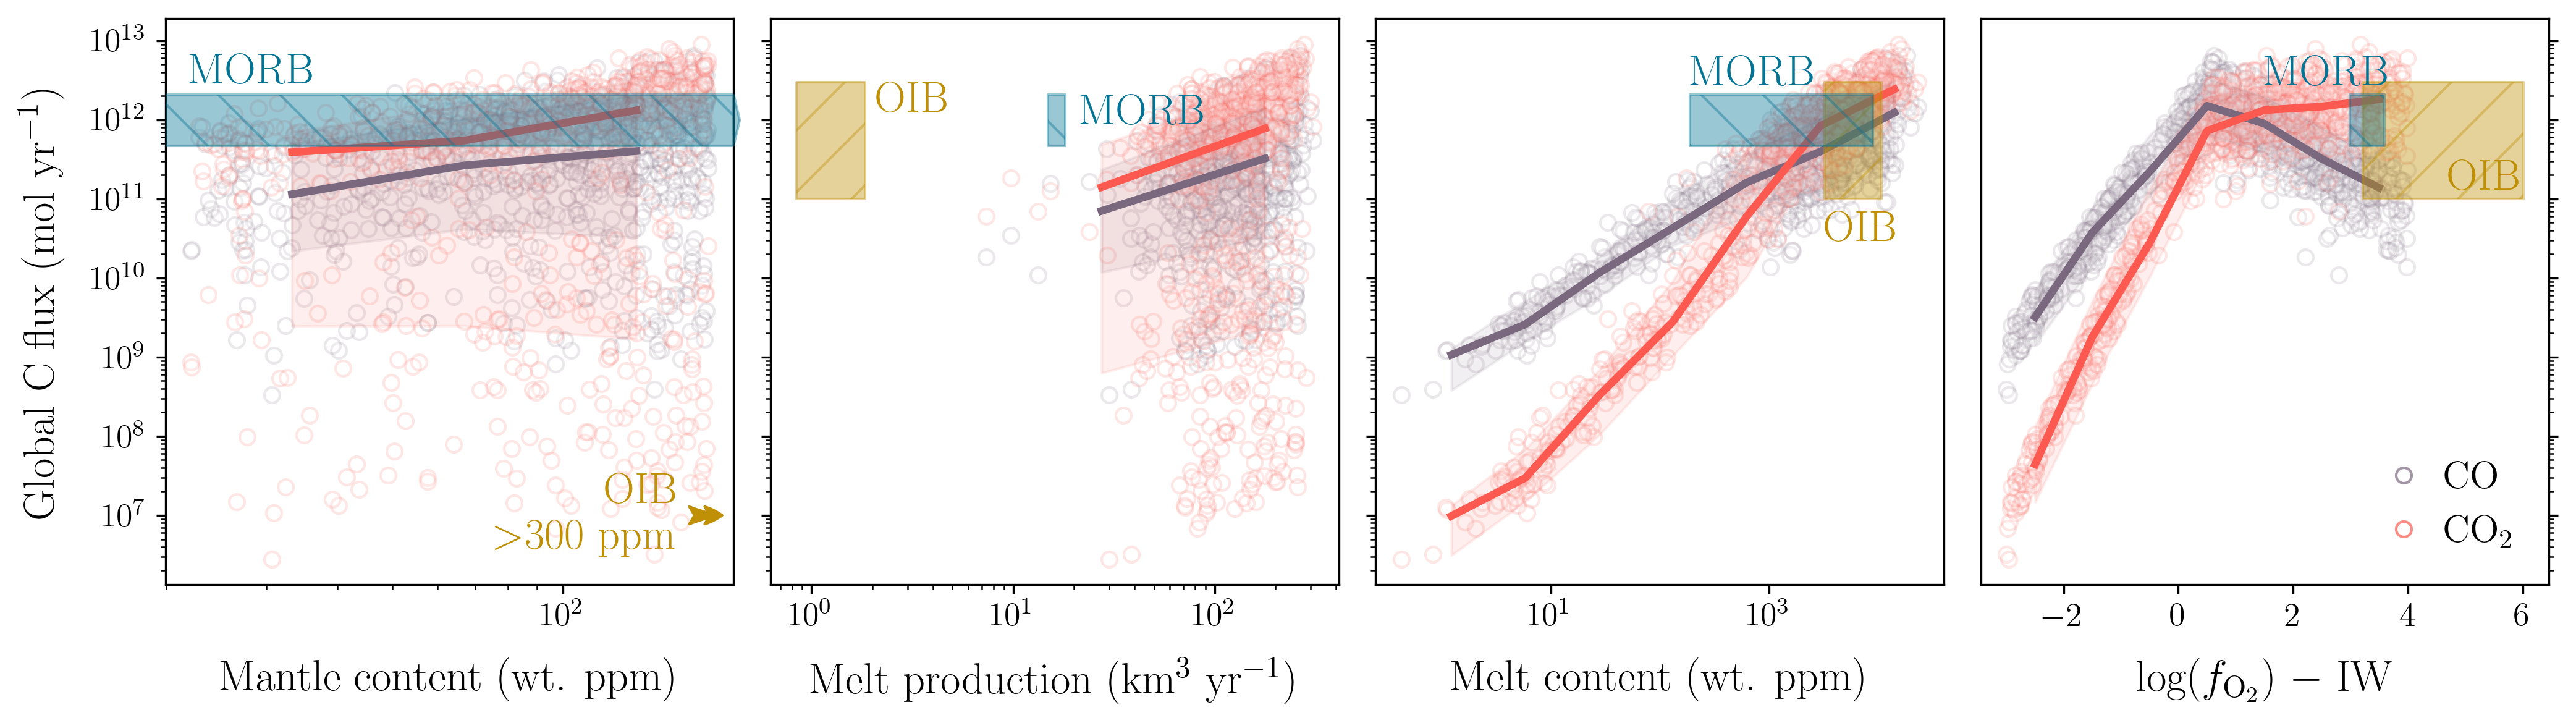
\includegraphics[width=1\linewidth]{C_summary.png}} \\
    % \subfloat[]{\label{sublable2}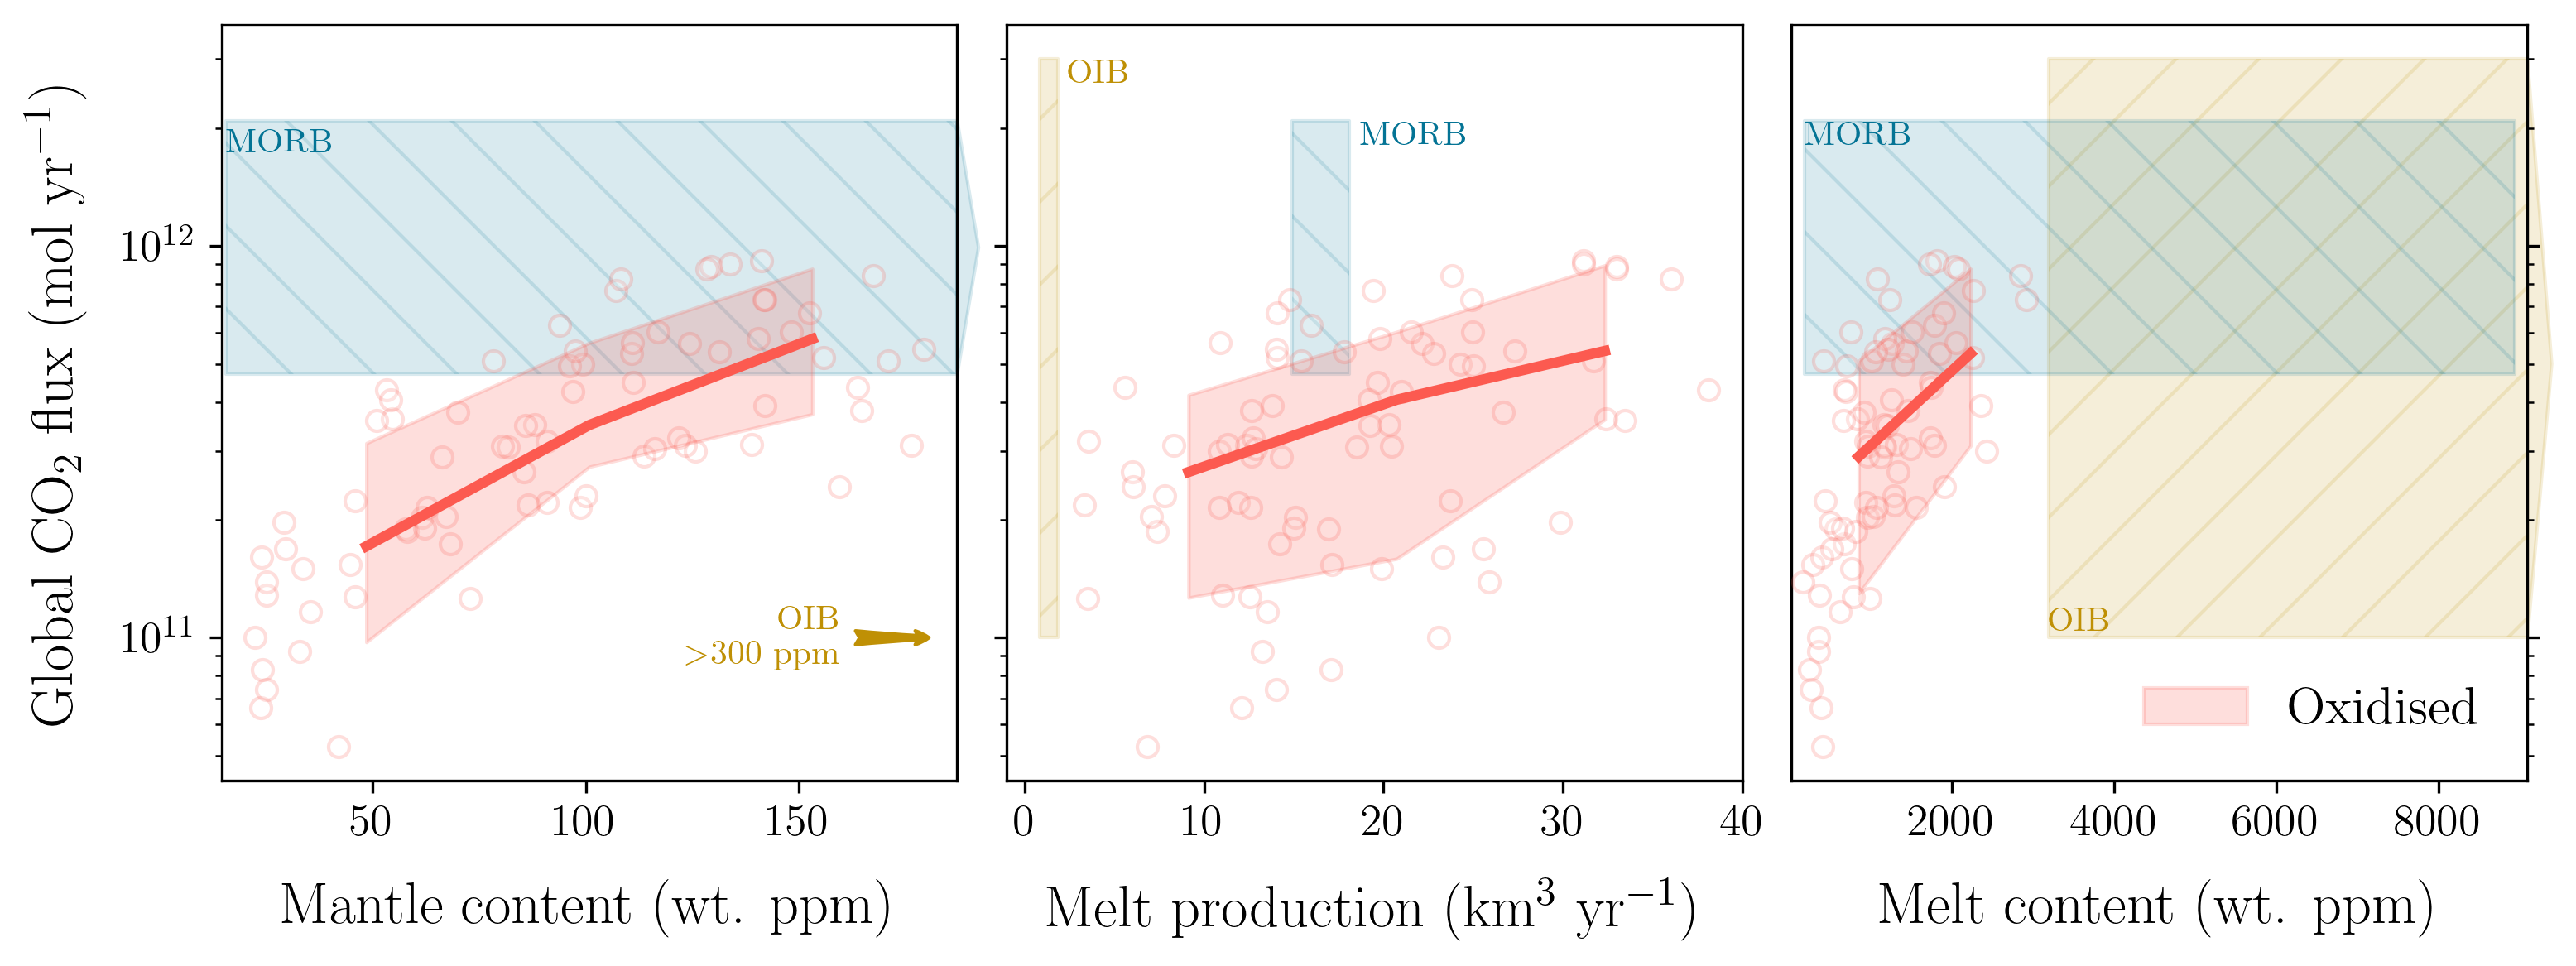
\includegraphics[width=0.75\linewidth]{C_summary_oxi.png}}
\caption[Summary of outgassing fluxes of CO and CO$_2$.]{\label{fig:summary_C}Summary of outgassing fluxes of CO (blue) and CO$_2$ (red), with respect to (from left to right) mantle source CO$_2$ content, melt production rate, melt CO$_2$ content, and mantle oxygen fugacity ($f_{\ch{O2}}$) relative to the iron-w\"ustite (IW) buffer. The mantle source concentrations in our model refer to the maximum (initial) values. All variables save $f_{\ch{O2}}$ are represented by the final 10-Myr mean. Each hollow circle denotes an individual model run. Solid lines show the median of all runs, and swaths show the 1$\sigma$ deviation. For context, we include estimates of modern Earth's CO$_2$ outgassing, spanned by blue rectangles for the mid-ocean ridge (MOR) system, and by beige rectangles for hotspots. MOR estimates are taken from the data in \citet{Voyer2019} and \citet{Hauri2019}, where the ranges of outgassing fluxes and melt production rates correspond to their quoted uncertainty on the global total, and the ranges of mantle and melt contents correspond to the 2$\sigma$-width of their log-normal sample distribution. For hotspots, the \ch{CO2} flux lower limit is the sum from major hotspots from \citet{Hauri2019}, and the generous upper limit is taken from \citet{Marty1998}; ocean island basalt (OIB) mantle source and melt concentrations are from \citet{Hauri2019}; magma supply rates are the sum over 19 hotspots from \citet{Mjelde2010}. Estimates of the mantle source $f_{\rm O_2}$ are from \citet{ONEILL2018} and \citet{AMUNDSEN1992} for MORB and OIB respectively. 
}
\end{figure}

\begin{figure}
\centering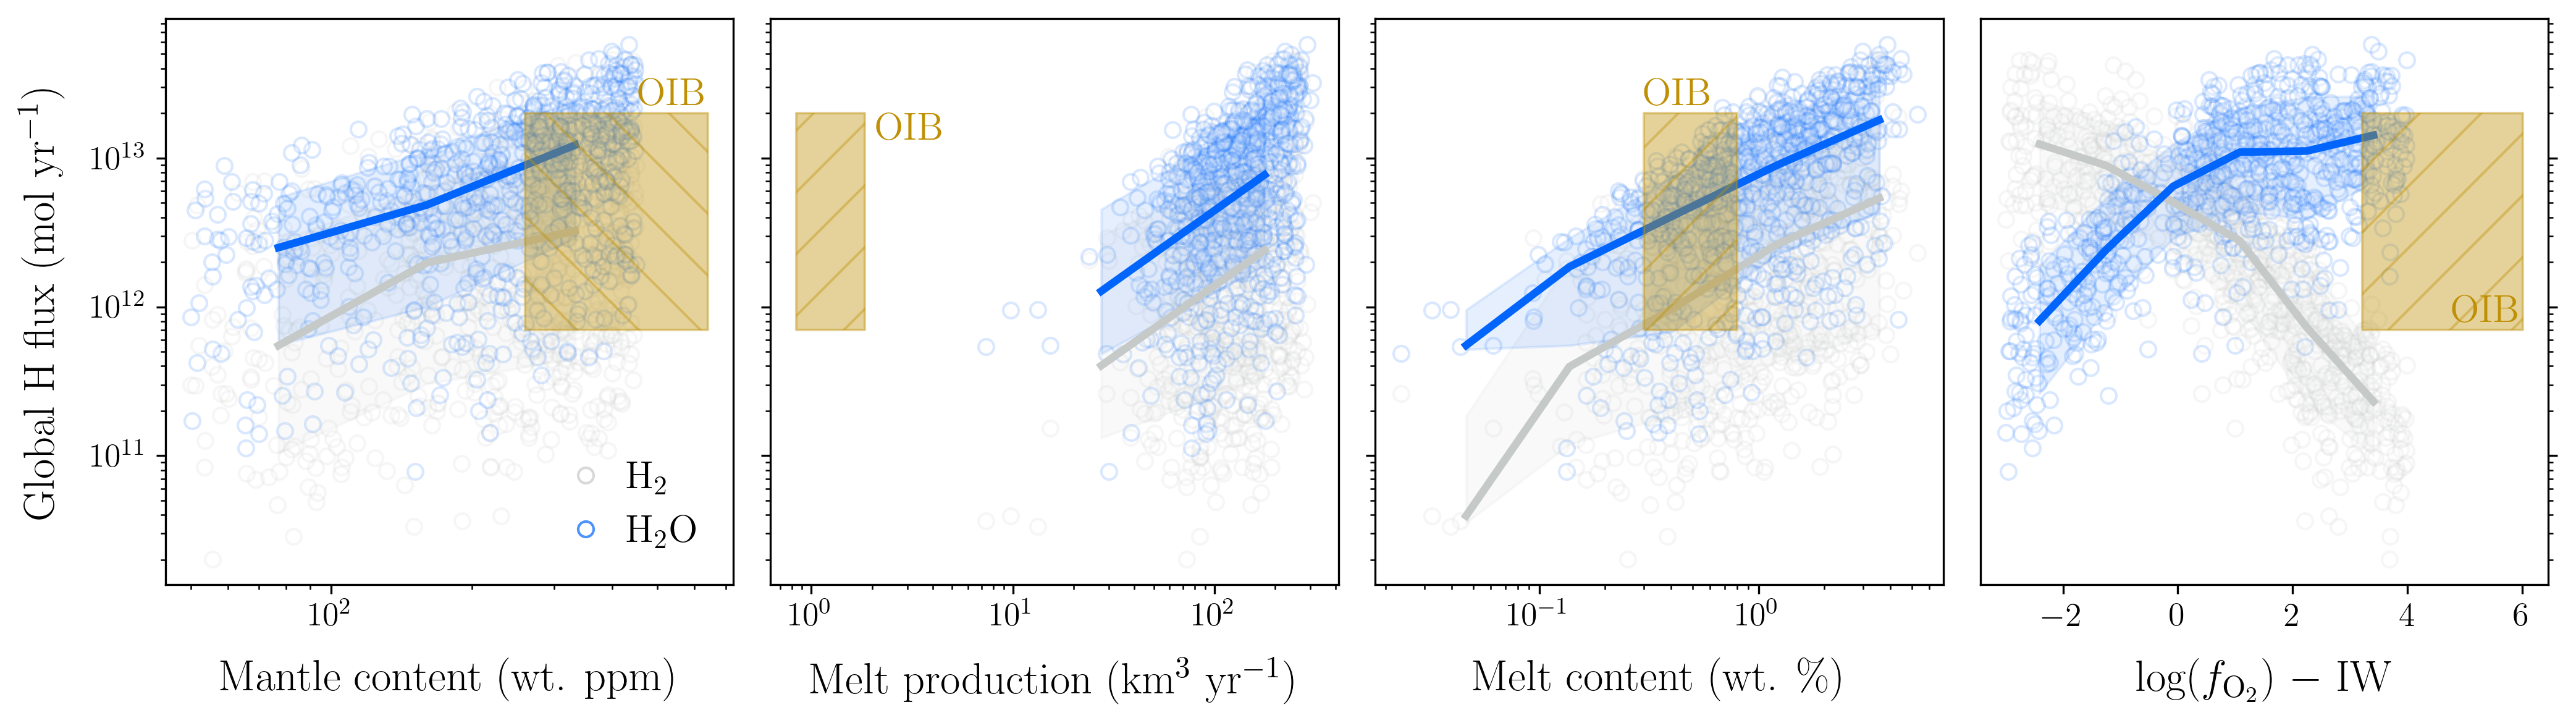
\includegraphics[width=1\linewidth]{H_summary.png}
\caption[Analogous to Fig. \ref{fig:summary_C}, but for H-bearing species.]{\label{fig:summary_H}Analogous to Fig. \ref{fig:summary_C}, but for H-bearing species, with H$_2$ flux in grey and H$_2$O flux in blue. The beige rectangle spans the estimate from \citet{DASGUPTA2010} for CO$_2$ hotspot volcanism, multiplied by 7--8, the typical ratio of H$_2$O to CO$_2$ in hotspot volcanic gas from \citet{Holland1984}; i.e., following \citet{Catling2017}. Mantle source concentrations refer to Hawaii estimates from \citet{Wallace1998}; melt concentrations are also Hawaii estimates from \citet{WallaceAnderson1998}. Mid-ocean ridge volcanism is omitted because it is known to be very dry, compared to the range shown here. Other data are explained in the caption to Fig. \ref{fig:summary_C}.}
\end{figure}

\subsubsection{Modern Earth's volcanic outgassing}


A key result from this work is that our stagnant lid outgassing model produces average outgassing rates no higher than those estimated for modern Earth under plate tectonics. Whereas $\sim$68\% of our cases more oxidised than IW + 3 have a \ch{CO2} flux of between 0.6 and 4.1 Tmol~yr$^{-1}$, estimates for Earth's global \ch{CO2} outgassing now rest at around $8.5 \pm 2$~Tmol~yr$^{-1}$ \citep{Catling2017}. Metamorphic degassing and arc volcanism, irrelevant to a stagnant lid regime, both account for a quarter of this global estimate. Although our model does not necessarily apply to hotspot or mid-ocean ridge outgassing in a plate tectonics regime either, estimates of the modern rates of these processes might provide a useful point of context for illustrating the mechanisms that keep our outgassing results relatively low.



Namely, we see four main factors potentially influencing outgassing: mantle volatile content, melt production rates, melt volatile contents, and mantle oxidation state. To this end, Figs. \ref{fig:summary_C} and \ref{fig:summary_H} summarise our modelled outgassing rates as a function of these four factors, overplotted by the relevant present-day estimates for hotspot and ridge volcanism. 


It should be noted upfront that our model may not be able to correctly capture modern ridge and hotspot outgassing rates, especially for \ch{CO2}. As explained in section \ref{sec:stagnant-lid} above, these processes sample recycled material generally having both (i) higher oxidation states, at the FMQ buffer or above \citep{AMUNDSEN1992, MOUSSALLAM2016, ONEILL2018, MOUSSALLAM2019}, to which our carbon partitioning model does not apply, and (ii) higher source volatile concentrations than our quasi-primordial bulk mantle values \citep{Hauri2019}. The combined effect of (i) and (ii) is that \ch{CO2} can potentially reach much higher melt concentrations on average. In oxidised conditions where carbonate is stable, abundant carbon would be lost very efficiently during partial melting.



Further to this point, modern outgassing rates are quite difficult to measure. Most quoted outgassing rates come from multiplying estimates of the melting rate with estimates of the concentration of volatiles in the melt. The volatile contents of melts are largely uncertain because melts are partially degassed; estimates rely on the behaviour of geochemical proxies \citep[see][]{Michael2015}. An in-depth review of Earth's ridge and hotspot outgassing rates is well beyond the scope of this work.

\paragraph{Mantle oxidation state} Although measurements of mantle $f_{\ch{O2}}$ on modern Earth show spatial heterogeneities and generally becomes more reducing with depth, most magmas associated with arc, mid-ocean ridge, and hotspot volcanism are within about a log-unit of FMQ \citep[e.g.,][]{gaillard_diverse_2021}, and as such we can consider Earth's volcanic gases to be generally poor in CO and H$_2$.

\paragraph{Melt production} Estimates of globally-integrated magma supply rates at mid-ocean ridges tend to show better agreement---most not far from 20 km$^3$ yr$^{-1}$ \citep{Crisp1984, Mjelde2010, Voyer2019}---although these estimates refer to the volume of all melt contributing to crust production, which may not necessarily be the same as the volume of melt contributing to outgassing. This study has found stagnant lid extrusive melting rates up to tenfold higher. Therefore melting rates alone would not explain our model's low outgassing fluxes. Hotspots are more geographically sparse, and their global magma supply rate is lower than ridges.


\paragraph{Mantle concentrations} The ridge mantle source shows orders-of-magnitude variation in \ch{CO2} concentrations (as derived from melt concentrations). This variation, extending from a minimum of 10~ppm to a maximum of 1980~ppm \citep{Hauri2019}, encompasses our entire range of $\chi_{\ch{CO2}}^{\rm{ini}}$. The hotspot mantle source tends to be even more volatile-rich, up to well over 1000~ppm in \ch{CO2}, and several hundred ppm for \ch{H2O} \citep{Wallace1998, MILLER2019}.


\paragraph{Melt concentrations} Our oxidised cases overlap fairly well with estimates of the typical volatile concentrations in modern ridge and hotspot magmas, as well as with the corresponding outgassing fluxes. Simulations that reach higher $\chi_{\ch{CO2}}^{\rm melt}$ and $\chi_{\ch{H2O}}^{\rm melt}$, with respect to modern Earth, accordingly tend to produce higher \ch{CO2} and \ch{H2O} outgassing rates. However, for many of our simulations, the mantle is almost completely depleted in volatiles by 700~Myr. Thus even if the convective velocity is increased by a reduction in viscosity, for example, we would not expect outgassing rates to increase any further.





\vspace{0.4cm}
In summary, the most reliable way to attain higher outgassing rates in our stagnant lid model would be to raise the volatile content of the melt. However, a volatile-rich melt is not necessarily attainable by tweaking model parameters because the melt partitioning of \ch{CO2} and \ch{H2O} will be ultimately limited by their stocks in the upper mantle source. To illustrate what a stagnant lid regime's lower interior volatile supplies mean for possible outgassing rates: a mantle with $\chi_{\ch{CO2}}^{\rm ini} = 180$~ppm and no return fluxes could outgas a maximum of $\sim$16 bar \ch{CO2} at 30\% depletion and $\chi_{\rm extr}$ = 40\%. Meanwhile, outgassing 8.5 Tmol~yr$^{-1}$ \ch{CO2} \citep{Catling2017} over 1 Gyr is equivalent to a cumulative $\sim$75 bar.




\subsubsection{Archean outgassing proxies}

Few observational constraints exist on Archean outgassing rates. Xe isotope anomalies in Archean quartz suggest that mantle degassing was about tenfold greater at 3.3~Ga than at present \citep{Avice2017, martyGeochemicalEvidenceHigh2019}. This proxy would apply to C-O-H outgassing rates at 3.3~Ga if they were derived directly from magma production rates---indeed, these high melting rates suggested by Xe isotopes are matched by our stagnant lid model. However, the carbon and water contents of the melt are at least as important as the volume of the melt in determining C-O-H outgassing rates. 


\subsection{Implications for the Archean Earth system}\label{sec:implications}

\subsubsection{From outgassing to atmospheric composition}
\label{sec:atmosphere-discussion}

The atmospheric composition and oxidation state do not mimic the volcanic gas composition or  oxidation state: photochemical reactions and H escape can oxidise reduced gases, and extraterrestrial impactors could provide significant reducing power \citep{Zahnle2020}. In addition, it is possible that an earlier atmosphere degassed from the magma ocean was in some part still present at the end of the Hadean \citep{Hamano2013, Nikolaou_2019, Stueken2020}. We do not model the atmospheric composition here because its complexities deserve more astute attention. However, to build our discussion of this work's potential implications for the Archean Earth system, we will briefly contextualise our results alongside previous work. We focus on processes affecting the partial pressure of \ch{CO2} due to its importance in long-term climate stability.



The equilibrium between outgassing sources and silicate weathering sinks (seafloor and subaerial) controls $p$\ch{CO2}. Weathering is thought to regulate the surface temperature via a negative feedback loop: in the classic \citet{Walker1981} framework, there would be a single equilibrium combination of $p$\ch{CO2} and surface temperature for fixed values of the outgassing flux and other relevant parameters (e.g., the weatherable surface area). Lower outgassing---all else being equal---implies a cooler climate, a weaker need to weather, and a lower \ch{CO2} weathering flux \citep[e.g.,][]{Kadoya2014, KT2018}. For example, \citet{KT2018} find $p$\ch{CO2} between 2--500~mbar for a contemporaneous outgassing rate of 3--9~Tmol yr$^{-1}$ (95\% confidence intervals). According to that model, $p$\ch{CO2}~$< 2$~mbar might therefore be anticipated for less than 3~Tmol yr$^{-1}$ of outgassing; such rates are not ruled out by this study. Note that this $p$\ch{CO2} estimate assumes that weathering is not limited by mineral supply, and following equation (29) in \citet{foley_carbon_2018}, the supply limit to silicate weathering would only be reached at \ch{CO2} fluxes well over 100~Tmol yr$^{-1}$ in stagnant lid scenarios (i.e., it is not reached). For comparison, proxy analyses by \citet{Hessler2004} give a lower limit of $p$\ch{CO2} $\sim 2.5$~mbar at at 3.2~Ga.






\subsubsection{Greenhouse warming under the Faint Young Sun}

Despite the fainter luminosity of the young sun, geochemical evidence exists for a temperate climate and stable oceans on Earth as early as 4.4~Ga \citep[e.g.,][]{Wilde2001, Valley2002, Valley2014}. Attempts to explain this paradox often invoke stronger-than-modern atmospheric partial pressures of greenhouse gases \citep[see review in][]{charnay2020}. Volcanic outgassing, being the main source of these greenhouse gases, is a primary control on steady-state $p$\ch{CO2} and surface temperature \citep[e.g.,][]{Walker1981, Sleep2001, Kadoya2014, honing_carbon_2019}. 


Indeed, the \ch{CO2} outgassing rates predicted here are at best several times lower than the values often assumed in Archean Earth climate models \citep[e.g.][]{Sleep2001, Wordsworth2013, CHARNAY2017, KANZAKI2018, KT2018}. These higher rates might relate to some combination of a different tectonic mode at the time, a higher extrusive volcanism percentage, and a more-oxidised mantle. 



3D general circulation models can be used to estimate the minimum partial pressures of \ch{CO2} that would provide the necessary greenhouse warming, for a given solar luminosity. For example, \citet{Wolf2014} find that maintaining 15\degree C requires $\sim$200~mbar of \ch{CO2} at 3.8~Ga, if other climate parameters (e.g., day length) are not optimal, and tens of mbar if they are. Note that this smaller value is similar to the minimum $p$\ch{CO2} from the low-outgassing scenarios studied by \citet{KT2018}. Dedicated atmospheric modelling should estimate the feasibility of greenhouse warming fed by weaker outgassing in the early Archean. 

At the least, if a planetary mantle $f_{\ch{O2}}$ were below the IW buffer, then it is apparent that virtually no \ch{CO2} could be outgassed in principle, even with melting rates much higher than estimated here. Indeed, silicate Earth may have already reached $f_{\ch{O2}} > {\rm IW} + 1$ by the end of the Hadean \citep{Pahlevan2019}. Depending on the longevity of the primordial magma ocean atmosphere, requiring a \ch{CO2} outgassing rate of at least several Tmol yr$^{-1}$ to sustain an early greenhouse may lend a constraint on the timing of mantle oxidation.


\section{Conclusions}

This work has coupled a 2D numerical model of stagnant lid convection with melting, volatile partitioning into the melt, and chemical speciation of these volatiles. The model returns redox-dependent volcanic outgassing fluxes of \ch{CO2}, \ch{CO}, \ch{H2O}, and \ch{H2}. We have applied this model to Hadean-Archean Earth. We find global \ch{CO2} and \ch{H2O} outgassing fluxes on the order of 1 Tmol yr$^{-1}$ and 10 Tmol yr$^{-1}$ respectively, depending on the mantle oxidation state. These fluxes are kept low by the assumption of a stagnant lid regime, wherein outgassing may never be much stronger than predicted here if the upper mantle cannot be efficiently replenished in volatiles. Our model may not apply to a scenario where most outgassing occurred on the seafloor, or where the upper mantle were too oxidised for graphite to be the stable form of carbon.


Coupled convection-outgassing models could inform further studies of the early Earth's atmospheric evolution. In particular, unknown \ch{CO2} outgassing rates throughout the late Hadean and early Archean account for a significant portion of the uncertainty on the contemporaneous greenhouse warming capacity. Previous estimates of Earth's climate state during the early period of lower solar luminosity tend to employ outgassing rates higher than the present day, an assumption which might not be substantiated given the unknown tectonic state. If we believe that the presence of surface liquid water in the early Archean demands fairly high \ch{CO2} partial pressures \citep{charnay2020}, then coupled outgassing models might test whether an early initiation of plate tectonics---combined with rapid mantle oxidation---may be key to building a temperate young planet.



\vspace{2cm}

\subsection*{Acknowledgements}

This manuscript has been markedly improved by the feedback of two anonymous reviewers. Their effort and their insight were critical in every sense, as were the editor's. The authors would like to thank the HPC Service of ZEDAT, Freie Universit\"{a}t Berlin, for computing time. This work was funded by the Deutsche Forschungsgemeinschaft (DFG, German Research Foundation) -- Project-ID 263649064 -- TRR 170. This is TRR 170 Publication No. 142. CMG has received additional funding from the University of Cambridge Harding Distinguished Postgraduate Scholars Programme and the Natural Sciences and Engineering Research Council of Canada (NSERC). Cette recherche a \'{e}t\'{e} financ\'{e}e par le Conseil de recherches en sciences naturelles et en g\'{e}nie du Canada (CRSNG). CMG thanks R. J. Graham and J. Krissansen-Totton for useful discussion, as well as her PhD supervisors O. Shorttle and J. F. Rudge for their patience with this project. 




%!TEX root = ../thesis.tex
%*******************************************************************************
%****************************** Third Chapter **********************************
%*******************************************************************************
\chapter{Mantle mineralogy limits to rocky planet water inventories}
\label{chapter:rockywater}

% **************************** Define Graphics Path **************************
\ifpdf
    \graphicspath{{Chapter3/Figs/Raster/}{Chapter3/Figs/PDF/}{Chapter3/Figs/}}
\else
    \graphicspath{{Chapter3/Figs/Vector/}{Chapter3/Figs/}}
\fi

\nomenclature[a-ffe]{$f^{\rm Fe}_{\rm mantle}$}{molar fraction of iron in mantle to total iron in bulk planet}
\nomenclature[a-xh]{[X/H]}{logarithmic stellar abundance ratio of an element X to hydrogen and normalised to the solar value.}
\nomenclature[z-mtz]{MTZ}{mantle transition zone}
\nomenclature[z-nam]{NAM}{nominally anhydrous mineral}
\nomenclature[z-cmb]{CMB}{core-mantle boundary}
\nomenclature[a-radius]{$r$}{radius [m]}
\nomenclature[a-g]{$G$}{gravitational constant [${\rm m^3 \, kg^{-1} \, s^{-2}}$]}
\nomenclature[a-h]{$\Delta H^{\rm 1 bar}$}{reaction enthalpy at 1 bar [${\rm J \, mol^{-1}}$]}
\nomenclature[a-v]{$\Delta V^{\rm solid}$}{reaction volume change of solids [${\rm m^3 \, mol^{-1}}$]}
\nomenclature[a-fzw]{$f_{\ce{H2O}}$}{water fugacity}
\nomenclature[a-c]{$c_{\ce{H2O}}$}{concentration by weight of water at water saturation (in mineral)}
\nomenclature[a-d]{$D$}{ratio describing partitioning of a component (usually water) between two phases}
\nomenclature[a-w]{$w$}{water mass at water saturation (in planetary mantle) [kg]}
\nomenclature[a-tempx]{$T_p$}{potential temperature [K]}
\nomenclature[z-om]{OM}{ocean mass, value for Earth's surface ocean [kg]}
\nomenclature[z-um]{UM}{upper mantle}
\nomenclature[z-um]{LM}{lower mantle}
\nomenclature[z-obm]{OBM}{olivine-bearing mantle}


\section*{Preface}

This chapter was published under the same title in \textit{Monthly Notices of the Royal Astronomical Society} in January 2023, appearing in the bibliography as \citet*{guimond_mantle_2023}. After a short note on author contributions, it is presented here reformatted, but otherwise unaltered except for minor notation changes conforming to the rest of the thesis.


\subsubsection*{Contributions and context}

I acknowledge the article's coauthors Oliver Shorttle and John Rudge. Oli encouraged me to exoplore exoplanet interiors using petrological models, which have recently entered the literature in the context of calculating mass-radius relationships. This study is one of the first to apply these models to comparative planetary evolution. John provided feedback on the interior structure equations, among other things. Both of these people have critically supported me as this chapter was written, and through their supervison, improved the quality of the science overall. This article has undergone peer review.




\section*{Abstract}
Nominally anhydrous minerals in rocky planet mantles can sequester multiple Earth-oceans' worth of water. Mantle water storage capacities therefore provide an important constraint on planet water inventories. Here we predict silicate mantle water capacities from the thermodynamically-limited solubility of water in their constituent minerals. We report the variability of upper mantle and bulk mantle water capacities due to (i) host star refractory element abundances that set mantle mineralogy, (ii) realistic mantle temperature scenarios, and (iii) planet mass. We find that transition zone minerals almost unfailingly dominate the water capacity of the mantle for planets of up to $\sim$1.5 Earth masses, possibly creating a bottleneck to deep water transport, although the transition zone water capacity discontinuity is less pronounced at lower Mg/Si. The pressure of the ringwoodite-perovskite phase boundary defining the lower mantle is roughly constant, so the contribution of the upper mantle reservoir becomes less important for larger planets. If perovskite and postperovskite are relatively dry, then increasingly massive rocky planets would have increasingly smaller fractional interior water capacities. In practice, our results represent initial water concentration profiles in planetary mantles where their primordial magma oceans are water-saturated. This work is a step towards understanding planetary deep water cycling, thermal evolution as mediated by rheology and melting, and the frequency of ocean planets.




\section{Introduction}

Water has a major effect on planetary processes, from their deepest interiors to their surfaces and atmospheres. In a planet's atmosphere, water is likely to be both the major greenhouse gas species and source of clouds, critical therefore for climate and atmospheric dynamics \citep[e.g.,][]{pierrehumbert_thermostats_1995,frierson_grayradiation_2006,frierson_grayradiation_2007}. At the surface, the amount of water trades off with topography to determine whether or not continents are exposed \citep{cowan_water_2014, honing_continental_2016, guimond_blue_2022}. In extreme cases, planets with high surface water inventories will be ocean worlds, presenting possible challenges for volatile cycling \citep{kitzmann_unstable_2015, noack_waterrich_2016, nakayama_runaway_2019, honing_carbon_2019, krissansen-totton_waterworlds_2021}, prebiotic chemistry \citep{patel_common_2015, rimmer_origin_2018}, and the detection of any biotic \ce{O2} \citep{glaser_detectability_2020, krissansen-totton_oxygen_2021}. Even water sequestered far below the surface can have a profound influence on planetary evolution: water changes the mantle rheology (i.e., viscosity) and so the thermal evolution of the interior \citep{karato_rheology_1993, seales_deep_2020}; it facilitates mantle melting by lowering the mantle solidus and so promotes volcanism \citep{green_experimental_1973, katz_new_2003}; and it may be responsible for the initiation of plate tectonics and the birth of continents on Earth \citep{korenaga_initiation_2013}. Water's multitudinous influence throughout planets demonstrates that it is not only the total budget of water that matters for habitability---the partitioning of water between the planet's surface and interior is crucial as well.

Although we may never answer how much water an exoplanet carries in its interior at a given time, we can place some constraints. Solid planetary mantles have thermodynamic limits to water saturation; their total water \textit{capacities} follow deterministically from known and measurable parameters. Further, as upper limits, these are physically meaningful, for they approximate the water budget of a planet's mantle shortly after its formation: primordial mantles may inherit large inventories of water as they crystallise from magma oceans overlain by thick steam atmospheres \citep{tikoo_fate_2017, dorn_hidden_2021, bower_retention_2021, miyazaki_wet_2022, salvador_convective_2023}. In these water-saturated conditions, the solubility of water in hot, newly-solidified mantles provides the initial condition for subsequent water cycling---a particularly important bound for stagnant lid planets lacking an efficient return flux of volatiles to the mantle \citep[e.g.,][]{foley_carbon_2018}. The maximum water capacity of the mantle under a stagnant lid gives a hard upper limit on the ocean mass that it could outgas over geologic time. On young planets, rates of total outgassing also correlate more strongly with the initial water content of the mantle than its temperature \citep{guimond_low_2021}. This could matter, for example, on planets around M-dwarfs, if they must sequester water in their mantles or else lose it early on to space under high stellar XUV radiation \citep{wordsworth_water_2013, luger_extreme_2015, godolt_habitability_2019, fleming_xuv_2020, moore_keeping_2020}; replenishment of any surface oceans may be limited by mantle water capacity.


To make a quantitative estimate of interior water capacities, we consider ``water'' not present as \ce{H2O}, but held as hydroxyl groups in the crystal structure of the nominally-anhydrous minerals (NAMs), such as olivine, that make up the mantle. That is, OH exists only in defects in the mineral, rather than as a stoichiometric component. Each NAM has a thermodynamically-limited water capacity, beyond which defects in the crystal are saturated, and additional water added to the system would be present as a free-water phase. The maximum water storage capacity of a planet's mantle is therefore determined by its mineralogy, and by those minerals' respective water capacities. Although planets have another large reservoir of H in their cores, our study does not count core H towards the interior water capacity because this reservoir is unlikely to participate in subsequent planetary evolution.
%Therefore, despite observational degeneracy, and despite the uncertainty in stochastic water accretion models \citep[e.g.,][]{morbidelli_source_2000, burger_realistic_2020}, a constraint on planetary water inventories can be found by way of mineralogy.


A planet's mantle mineralogy, in turn, depends on its elemental composition, pressure, and to a lesser extent, temperature. This elemental composition is set during formation, by a planet's building blocks, which themselves are linked ultimately to the composition of the system's natal molecular cloud \citep{anders_solarsystem_1982, thiabaud_elemental_2015, bonsor_hoststar_2021}. Therefore exoplanet mantle mineralogies are predicted in tandem with \textit{(i)} measurements of stellar refractory element abundances and \textit{(ii)} models calculating the equilibrium mineralogy for a given composition, pressure, and temperature \citep[e.g.,][]{connolly_geodynamic_2009}, as has been investigated extensively in the literature \citep{dorn_can_2015, dorn_bayesian_2017, dorn_generalized_2017, dorn_new_2019, unterborn_effects_2017, unterborn_nominal_2023, hinkel_star_2018, otegi_impact_2020, spaargaren_influence_2020, spaargaren_plausible_2022, wang_detailed_2022}. In particular, the ratio of the two most abundant refractory lithophile elements, Mg to Si, has a first-order effect on mineralogy \citep[e.g.,][]{dorn_bayesian_2017, unterborn_effects_2017, hinkel_star_2018, wang_enhanced_2019, spaargaren_influence_2020, spaargaren_plausible_2022}. We thus expect Mg/Si to control a planet's mantle water storage capacity as an outcome of stellar nucleosynthesis. Overall mineral proportions will also depend on planet size, as high-pressure mineral phases (e.g., postperovskite) make up a large volume of Earth-sized and larger planets. The wide range in water solubility across NAMs, stable at certain characteristic pressures, means that water capacity will not scale linearly with planet mass.

In pursuit of constraints on the water capacity of Earth's mantle, the last two decades saw several efforts compiling the experimental and theoretical constraints on NAM water solubilities \citep[e.g.,][]{keppler_thermodynamics_2006, ohtani_hydrous_2015, demouchy_distribution_2016, tikoo_fate_2017, dong_constraining_2021, andrault_mantle_2022}. Disagreement may persist for some minerals---high-pressure phases in particular---yet there seems to be a robust shape to the mantle water saturation profile overall. Its most obvious feature is distinct discontinuities where (Mg, Fe)$_2$SiO$_4$ olivine transitions to its high-pressure polymorph wadsleyite, and again where the yet higher-pressure olivine polymorph ringwoodite dissociates to (Mg, Fe)SiO$_3$ perovskite. The olivine-bearing part of the upper mantle tends to have lower water saturation, mostly on the order of hundreds of parts per million by weight (but increasing with pressure). The appearance of wadsleyite marks the mantle transition zone (MTZ); here, water saturations leap to the weight-percent level. The beginning of perovskite stability marks the start of the lower mantle, which most studies find to be drier again---a few experiments have found high perovskite water saturations of $\sim$1 wt.\%, however \citep{murakami_water_2002, fu_water_2019}. As a consequence, the MTZ is not just a reservoir for water, but also a key structural feature of the deep water cycle: \textit{(i)} the ringwoodite-perovskite transition acts as a bottleneck for water transport down to the drier, deeper mantle; and, \textit{(ii)} upward flow across the wadsleyite-olivine transition acts as a source of hydrous magma by dehydration melting \citep{bercovici_wholemantle_2003, andrault_mantle_2022}. A key question in the context of exoplanets is whether the distinct mantle water reservoirs on Earth are ubiquitous among rocky planets.

Important work has already been undertaken investigating mantle water capacities beyond Earth. \citet{shah_internal_2021} calculated the water saturation of idealised mantles with fixed NAM compositions in the Mg-Fe-Si system, with varying planet mass and potential temperature. The aim of \citet{shah_internal_2021} was to show that distinguishing a fully-saturated mantle from a water-free one is not possible from planet mass/radii observations, since realistic amounts of water stored in a solid mantle does not significantly affect its bulk density. More recently, \citet{dong_water_2022} quantified Mars' mantle water capacity given constraints on its particular bulk composition. We build on these two studies by exploring water capacities over a wide range of possible mantle Mg-Fe-Si-Ca-Al bulk compositions estimated from the Hypatia Catalog of FGKM star element abundances \citep{hinkel_stellar_2014}. %Approaching planetary water budgets from the perspective of the mantle complements other estimates based on accretion and loss processes in the nebular atmosphere \citep[e.g.,][]{kimura_formation_2020}. 
% As mantle water capacities, and their dependence on the [xo?]planets mass, have not been previously quantified, existing planetary water cycling models typically either do not scale planetary water capacity with mass, or do so based on approximate scalings from Earth \citep[e.g.,][]{cowan_water_2014, schaefer_persistence_2015, komacek_effect_2016, moore_keeping_2020}. 
Because the diversity of mantle water capacities has not been quantified, previous rocky planet water cycling models often use approximate Earth values for their initial conditions and mantle water saturation limits \citep[e.g.,][]{cowan_water_2014, schaefer_persistence_2015, komacek_effect_2016, moore_keeping_2020}. %In particular, interim scalings for mantle water capacity as a function of planet mass may be simplistic because they cannot account for the distinct water saturation limits of upper versus lower mantle NAMs.

This paper builds a method to convert stellar compositions into the interior water capacities of hypothetical rocky planets associated with those stars. In section \ref{sec:methods_comp}, we translate stellar element abundances into planetary oxide bulk compositions. In section \ref{sec:methods_structure}, we self-consistently calculate interior structures and mantle mineralogies from these bulk compositions, as a function of planet mass and potential temperature. Section \ref{sec:methods_sat} then describes how we use mineral water saturation data to estimate interior water capacities. We present our calculated distribution of rocky planet water capacities in section \ref{sec:results-water}. To end, section \ref{sec:discussion-water} discusses the implications for whole-planet water cycling and the propensity of waterworlds.   


\section{Methods}

\subsection{From stellar abundances to planet bulk composition}\label{sec:methods_comp}

Our hypothetical planets are composed of a solid, pure Fe core and a silicate mantle of \ce{MgO}, \ce{SiO2}, \ce{Al2O3}, \ce{CaO}, and \ce{FeO}\footnote{This implicitly assumes that all oxidised iron exists as \ce{FeO} and not \ce{Fe2O3}, since we do not track mantle oxygen fugacity.} We expect these oxides to make up $\gtrsim$98\% by mass of all rocky exoplanet mantles \citep{putirka_composition_2019}. The planets we model inherit identical bulk metal ratios to their host stars. We assume that oxygen would be abundant enough to bond with Ca, Mg, Al, and Si such that they are fully present as oxides in the mantle---Fe is present in excess of available oxygen and hence produces a metal core to the planet. 

To specify the partitioning of total iron between Fe metal in the core and FeO in the mantle, we define \coreeff~as the molar ratio,
\begin{equation}\label{eq:core_eff}
    f^{\rm Fe}_{\rm mantle} = \frac{n_{\rm m}^{\rm Fe}}{n_{\rm m}^{\rm Fe} + n_{\rm c}^{\rm Fe}},
\end{equation}
where $n_{\rm m}^{\rm Fe}$ and $n_{\rm c}^{\rm Fe}$ are the number of moles of Fe in the mantle and core respectively.

For each planet-hosting FGKM star in the Hypatia Catalog\footnote{https://www.hypatiacatalog.com/} \citep{hinkel_stellar_2014}, including outliers, we find the mantle bulk composition and core mass fraction of hypothetical rocky exoplanets, depending on the star's measured elemental abundances and our choice of \coreeff. Specifically, we extract the number abundance of the rock-forming element X with respect to hydrogen, $n_{\rm X}/n_{\rm H}$, using the mean where multiple measurements exist. Hypatia reports logarithmic abundances, denoted ${\rm [X/H]}$, with respect to a solar normalisation:
\begin{equation}
    {\rm [X/H]} = \log(n_{\rm X}/n_{\rm H})_* - \log(n_{\rm X}/n_{\rm H})_{\sun},
\end{equation}
where the first term is the stellar value and the second is the solar value---here, that of \citet{lodders_abundances_2009}, as in \citet{hinkel_star_2018}. The corresponding list of $\left(n_{\rm X}/n_{\rm H}\right)_*$ can then be written as molar ratios of the metals in their respective oxide forms considering their stoichiometry; i.e., $n_{\rm Mg}:n_{\rm Si}:2n_{\rm Al}:n_{\rm Ca}:$ \coreeff$n_{\rm Fe}$. We convert these molar ratios to mass ratios of the respective oxides via molar mass and normalise to 100\%. As such, we make the simplification that these metals are equally refractory: whilst their absolute abundances in the bulk planet may not equal those in the stellar photosphere, we expect the ratios between them to be roughly preserved.  We do not propagate observational errors on stellar abundances, but a thorough discussion of this issue can be found in \citet{hinkel_star_2018} and \citet{hinkel_concise_2022}.

\subsubsection{Core mass fraction and partitioning of Fe}

We assume, in all cases, a pure iron core. The core mass fraction (CMF) is calculated from the mantle FeO content and \coreeff, conserving the bulk planet Fe content. We derive the CMF by the definition of \coreeff (\ref{eq:core_eff}):
\begin{equation}
\begin{split}
    n_{\rm m}^{\rm Fe} &= \frac{\chi_{\rm FeO} M_p \left(1 - {\rm CMF}\right)}{M_{\rm FeO}} \\
    n_{\rm c}^{\rm Fe} &= \frac{{\rm CMF} \, M_p}{M_{\rm Fe}},
\end{split}
\end{equation}
where $M_{\rm Fe}$ and $M_{\rm FeO}$ are the molar masses of Fe and FeO respectively in ${\rm kg}\,{\rm mol}^{-1}$, $M_p$ (which cancels out) is the mass of the planet in kg, and $\chi_{\rm FeO}$ is the mantle weight fraction of FeO. This has the analytical solution,
\begin{equation}\label{eq:CMF}
    {\rm CMF} = \frac{M_{\rm Fe} \chi_{\rm FeO} \left(1 - f^{\rm Fe}_{\rm mantle}\right)}{-M_{\rm Fe} \chi_{\rm FeO} f^{\rm Fe}_{\rm mantle} + M_{\rm Fe} \chi_{\rm FeO} +  M_{\rm FeO} f^{\rm Fe}_{\rm mantle}}.
\end{equation}
In this way, an Earth-like FeO mantle fraction \citep[8.05 wt.\%;][]{mcdonough_composition_1995} and core mass fraction (0.325) are equivalent to \coreeff$\,= 0.117$; \coreeff$\,= 0$ denotes an Fe-free mantle. 



% \todo{Note this maximum \coreeff of 0.5 gives 21.7\% FeO for solar composition; cf. Vesta is the highest in the SS at 24\% \citep{tronnes_core_2019}. 


%The actual amount of oxygen that condenses in refractory phases may depend on the planet's radial location of accretion in the disk and the systemic Mg/Si ratio, but in any case is not yet predictable \textit{a priori} \citep{unterborn_effects_2017}.
% khan value equals Mg# 0.81
% Also Perple\_X seems to break with Mg\# $\lesssim$ 0.6---getting super weird ringwoodite stability at 10 GPa. Have decided to use the perplex breaking limit as an endmember, will sort this soon, only matters for one figure.


We consider a generous range of \coreeff~from 0 to 0.3. The existence of core-free rocky planets has been proposed before, but these planets may require formation environments out beyond the snow line---where they can accrete very oxidised, water-rich material \citep{elkins-tanton_coreless_2008, kite_atmosphere_2020}. Our range of \coreeff~encompasses mantles more oxidising than Mars', which itself has had its FeO content recently revised from 17--18 wt.\% down to $\sim$14 wt.\% \citep{khan_geophysical_2022}, giving, in our pure-iron-core model, \coreeff~= 0.236 for a martian core mass fraction of 0.25. 

\subsubsection{Some initial caveats}

In performing these estimates, we are not aiming to predict in detail the composition of a particular planet's mantle, but rather to capture the possible variability in water storage capacity at a population level. Namely, planetary accretion and differentiation may involve several fractionation processes that modify the compositional relationship between star and planet. Being the most refractory out of the elements we consider, Al and Ca show no depletion on Earth with respect to solar abundances---our simplified method will therefore slightly underestimate the proportions of \ce{Al2O3} and \ce{CaO} relative to other oxides. For similar reasons we have excluded Na, a moderately volatile element that would fractionate more strongly with respect to the others, during condensation from the nebular gas and evaporation from molten planets (and is nevertheless an order of magnitude less abundant). 

Meanwhile, Mg, Si, and Fe are expected to have similar depletion ($\sim$14--20\%) between the star and bulk planet \citep{wang_enhanced_2019}---yet we know from Earth that solar Mg/Si ($=1.04$) is only a rough approximation of mantle composition as it fails to predict Earth's measured upper mantle Mg/Si of 1.25; somewhere, partitioning must be occurring \citep[see also section \ref{sec:discussion-sio2-water}]{ringwood_significance_1989, mcdonough_composition_1995, lodders_abundances_2009}. Nevertheless, despite knowing that in detail stellar Si abundances will not equal those in the planet, the exact processes leading to the incorporation of Si into a growing planet's mantle (or core) are not yet easily and deterministically quantifiable: they involve not just devolatilisation and dust transport in disks \citep{miyazaki_dynamic_2020}, but also the high-pressure core-mantle partitioning of Si \citep{fischer_high_2015}.

Further to mantle compositions, the cores of rocky planets may not be pure solid Fe. Cores could contain lighter elements, or be partially or entirely molten. Both phenomena would affect the core radius at a given CMF, and accordingly the pressure and temperature gradients of the mantle \citep{unterborn_scaling_2016}. Although these particular effects of changing core radius are inconsequential to our water capacity results, the principles are discussed in section \ref{sec:results_fe}. Note that if one of these light elements is Si, then the mantle mineralogy changes (section \ref{sec:discussion-sio2-water}). If one of them is H, then the core could in this way contribute to the total ``water'' capacity of the planet \citep{shah_internal_2021}. Nevertheless, the solubility of water in mantle minerals is independent from that in the core at water saturation. Even more importantly for planetary evolution, the core H reservoir is likely sealed from the surface following its formation, whereas mantle water may be released through volcanism.



\subsection{Interior structure and mineralogy}\label{sec:methods_structure}


To compute equilibrium mineral phase abundances given a bulk oxide composition, we use the Gibbs free energy minimisation code Perple\_X \citep{connolly_geodynamic_2009}. This code, with some extrapolation of thermodynamic properties, has previously been used to investigate the silicate mantles of planets up to 10 $M_\oplus$ \citep{dorn_can_2015, dorn_generalized_2017, dorn_new_2019, unterborn_inward_2018, hinkel_star_2018, unterborn_pressure_2019, otegi_impact_2020, wang_detailed_2022}. At the current time we are not able to consider the effect of water on sub-solidus phase boundaries, although experiments on water-present, Earth-like mantle compositions suggest a limited influence of water incorporation on NAM stability \citep[shifting the depth of phase boundaries by at most a few GPa;][]{litasov_influence_2006}.

Phase abundances, being a function of pressure and temperature, must be calculated along an adiabat from the surface to the core-mantle boundary. However, the adiabatic gradient depends in turn on the phases present. Therefore our model self-consistently finds the mantle pressure $P$, temperature $T$, and phase abundance profiles using an iterative method summarised in Figure \ref{fig:flowchart}. 


\begin{figure}
\caption[Flowchart for the iterative planetary interior model.]{Interior model iterative method. See text for symbol definitions and further details. \label{fig:flowchart}}
\centering
\begin{tikzpicture}[font=\small,thick]

\node[draw,
    rounded rectangle,
    minimum width=2.5cm,
    minimum height=1cm] (block1) {START};
    
    \node[draw, text width=4cm,
    trapezium, 
    trapezium left angle = 65,
    trapezium right angle = 115,
    trapezium stretches,
    below=of block1,
    minimum width=3.5cm,
    minimum height=1cm
] (block2) { Construct mass profile, define mantle and core regions. Set initial guesses for $\rho$, $\alpha$, $c_p$. };

\node[draw, text width=2cm,
    below=of block2,
    minimum width=1cm,
    minimum height=1cm
] (block3) { Calculate $r$, $g$, $P$, $T$ (\ref{eq:radius_prof}--\ref{eq:temperature_prof})};

\node[draw,  text width=3cm,
    diamond, aspect=2,
    below=of block3,
    minimum width=7cm,
    inner sep=0] (block4) { $P_{\rm CMB}$ converged with at least one iteration?};
        
        
        \node[draw,  text width=2.5cm,
    below left=of block4,
    minimum width=2.5cm,
    minimum height=1cm] (block5) { Update $\rho$, $\alpha$, $c_p$ in core region using hcp-Fe equation of state.};

\node[draw, text width=2.5cm,
    above left=of block4,
    minimum width=2.5cm,
    minimum height=1cm] (block6) { Update $\rho$, $\alpha$, $c_p$ in mantle region using Perple\_X.};
    
        \node[draw,  text width=2.5cm,
    below=of block4,
    minimum width=2.5cm,
    minimum height=1cm,] (block7) { Calculate water saturation profile.};

   
\node[draw,
    rounded rectangle,
    below=of block7,
    minimum width=2.5cm,
    minimum height=1cm,] (block8) { RETURN};
    
    % arrows
    \draw[-latex] (block1) edge (block2)
    (block2) edge (block3)
    (block3) edge (block4)
    (block7) edge (block8)
    (block5) edge (block6)
    (block6) edge (block3);
    
\draw[-latex] (block4) edge node[pos=0.4,fill=white,inner sep=2pt]{Yes}(block7)
    (block4) edge node[pos=0.3,fill=white,inner sep=0]{No} (block5);
    

\end{tikzpicture}
\end{figure}

Given an input planet mass, we subdivide a fixed mass profile, $m$ in kg, into $N$ equal shells from 0 to $M_p$, where $300 < N < 1600$ depending on $M_p$. At each iteration, we build the profiles of radius, $r$ in m, and gravity, $g$ in ${\rm m}\,{\rm s}^{-2}$, upwards from planet-centre boundary conditions of $r_0 = g_0 = 0$, 
\begin{equation}\label{eq:radius_prof}
r_n = \left(\frac{3\Delta m }{4 \pi \rho_n} + r_{n - 1}^3\right)^{\frac{1}{3}},
\end{equation}
\begin{equation}\label{eq:gravity_prof}
g_n = g_{n - 1} \left(\frac{r_{n - 1}}{r_n}\right)^2 + \frac{4 \pi G}{3} \rho_n \left(\frac{r_n^3 - r_{n - 1}^3}{r_n^2}\right)
\end{equation}
where $\Delta m = m_n - m_{n - 1}$ in kg (constant), $G$ is the gravitational constant in ${\rm m}^3 \, {\rm kg}^{-1}\,{\rm s}^{-2}$, and $\rho_n$ is the density of layer $n$ in ${\rm kg} \, {\rm m}^{-3}$.

We build the adiabatic $P$--$T$ profiles downwards from their near-surface boundary conditions: $P_s = 1000$~bar and a $T_s$ equal to the input potential temperature, $T_p$, in K:
\begin{equation}\label{eq:pressure_prof}
P_{n} = P_{n + 1} + \Delta r \, g_{n + 1} \rho_{n + 1},
\end{equation}
\begin{equation}\label{eq:temperature_prof}
T_{n} = T_{n + 1} + \Delta r \, \frac{\alpha_{n}g_{n}}{c_p,_{n}} T_{n + 1},
\end{equation}
where $\Delta r = r_n - r_{n - 1}$ in m, $c_p$ is the specific heat capacity in ${\rm J}\,{\rm kg}^{-1}\, {\rm K}^{-1}$ and $\alpha$ is the thermal expansivity in ${\rm K}^{-1}$; initial guesses for the mantle and core layers respectively are $1300\,{\rm J}\,{\rm kg}^{-1}\, {\rm K}^{-1}$ and $800\,{\rm J}\,{\rm kg}^{-1}\, {\rm K}^{-1}$ for $c_p$, and $2.5 \times 10^{-5}\,{\rm K}^{-1}$ and $1 \times 10^{-5}\,{\rm K}^{-1}$ for $\alpha$. Initial guesses for $\rho$ through the mantle and core layers are the average values from the parameterised interior structure of \citet{noack_parameterisations_2020}. For simplicity, we ignore any temperature jumps due to phase transitions or core heat transfer. 

We identify the core-mantle boundary pressure, $P_{\rm CMB}$, as the pressure at the layer $n$ where the cumulative mass reaches the pure-Fe core mass from (\ref{eq:CMF}): $\sum_n m_n \ge {\rm CMF} \cdot M_p$.


At subsequent iterations, we run Perple\_X to find the mineral phase mass fractions given both the mantle $P$--$T$ profile from the previous iteration, and the mantle bulk oxide composition from section \ref{sec:methods_comp}. The Perple\_X output consists of new $\rho$, $\alpha$, and $c_p$ profiles consistent with the calculated phase fractions. Our Perple\_X implementation uses the most recent mineral solution models and equations of state from \citet{stixrude_thermal_2022}. The 22-phase coverage of the \citet{stixrude_thermal_2022} database should be mostly complete for exoplanet mantles because wholly exotic bulk compositions are not expected \citep{putirka_composition_2019}. Note that other thermodynamic databases could result in different phase fractions; the \citet{stixrude_thermodynamics_2011} database, for example, produces a lower mantle with relatively less perovskite and more ferropericlase at an Earth-like bulk composition.

Above $200\,{\rm GPa}$, the thermodynamic data available to predict mantle mineralogy becomes very limited. Therefore, to avoid phase stability errors in the lower mantles of our calculated planets with $p_{\rm CMB} \ge 200\,{\rm GPa}$, we extrapolate constant mineralogies from $200\,{\rm GPa}$ to $p_{\rm CMB}$, although in this case we still calculate thermodynamic parameters using the same equations of state. At $M_p \gtrsim 3 M_\oplus$, the maximum mantle pressures found in our model start to surpass the theoretical pressures where Mg-postperovskite recombines with MgO or SiO$_2$ \citep{umemoto_phase_2017}. Whilst we still estimate a mantle water capacity for these higher-mass planets, we note that their lower mantle mineralogies will be much more uncertain. 

At pressures above $p_{\rm CMB}$, we calculate $\rho$, $\alpha$, and $c_p$ using a Holzapfel equation of state for pure hcp iron with parameters from \citet{bouchet_initio_2013} and \citet{hakim_new_2018}. 

Given the updated $\rho$, $\alpha$, and $c_p$, we re-calculate $r$, $g$, $P$, and $T$ (\ref{eq:radius_prof}--\ref{eq:temperature_prof}) to find the new adiabat, and so on. We stop the iteration when $p_{\rm CMB}$ has converged to within 0.01\%, which normally takes less than 10 iterations. This precision meets our needs, being, ultimately, to obtain $T$, $p$, $m$, and phase abundance profiles of a planet's mantle.


Our interior model is similar to ExoPlex \citep{unterborn_inward_2018}, and results in the same pressure, temperature, density, and phase gradients when using the same thermodynamic database.

\subsection{Mineral water solubility parameterisations}\label{sec:methods_sat}


\begin{table*}
\centering
\caption[Parameter values for the water saturation model.]{Water saturation model parameter values, either parameterised via (\ref{eq:c_h2o}) and (\ref{eq:D_ji}), or given mineral-mineral partitioning coefficients ($D$) or water concentrations ($c_{\rm H_2O}$). See text for details. \label{tab:saturation_params}}
\footnotesize
\begin{tabular}{@{} l r r r r    r r p{2.1cm}}
\toprule
 & \multicolumn{4}{c}{Parameters in (\ref{eq:c_h2o})} & \multicolumn{2}{c}{Data range} \\ \cmidrule(lr){2-5} \cmidrule(lr){6-7}
 
\multirow{2}{*}{Phase} & \multicolumn{1}{c}{$A$} & \multicolumn{1}{c}{\multirow{2}{*}{$n$}} & \multicolumn{1}{c}{$\Delta H^{\mathrm{1\,bar}}$} & \multicolumn{1}{c}{$\Delta V^{\mathrm{solid}}$} & \multicolumn{1}{c}{$T$} & \multicolumn{1}{c}{$P$} & \multirow{2}{*}{Ref.} \\

 & \multicolumn{1}{c}{$({\rm ppm\,bar^{-n}})$} & & \multicolumn{1}{c}{$({\rm kJ\,mol}^{-1})$} & \multicolumn{1}{c}{$({\rm cm^3\,mol}^{-1})$} & \multicolumn{1}{c}{$({\rm K})$} & \multicolumn{1}{c}{$({\rm GPa})$} & \\
 
\hline
\noalign{\vskip 1mm}
\multicolumn{8}{c}{$\bm{c}\mathbf{_{H_2O}}$ \textbf{calculated directly}} \\
\noalign{\vskip 1mm}

ol &  $4.6838\times 10^{-2}$ & 0.33235 & $-40.787$ & 0 & 1273--2273 & 1.8--14.5 & \citet{dong_constraining_2021}  \\  
wad &  $4.8295\times 10^{-4}$ & 0 & $-114.230$ & 0 & 1673--2273 & 13.5--20.0 & \citet{dong_constraining_2021}  \\  
ring & $1.0224\times 10^{-3}$ & 0 & $-101.482$ & 0 & 1673--2073 & 17--23 & \citet{dong_constraining_2021}  \\  
coes & \multicolumn{4}{c}{$T, p$-dependent $c_{\rm H_2O}$ (see text)} & 1073--1573 & 5.0--9.1 & \citet{yan_water_2021}  \\
stv & \multicolumn{4}{c}{$T, p$-dependent $c_{\rm H_2O}$ (see text)} & 1000--2000 & 0--60 & \citet{panero_hydrogen_2004} \\ 

\noalign{\vskip 1mm}
\hline
\noalign{\vskip 1mm}
\multicolumn{8}{c}{$\bm{c}\mathbf{_{H_2O}}$ \textbf{calculated using a parameterised partitioning coefficient with ol}} \\
\noalign{\vskip 1mm}

opx (en)$^{\ast\dagger\ddagger}$ & $1.354\times 10^{-2}$ & 1.0 & $-4.563$ & 12.1 & 1373 & 2--10 & \citet{rauch_water_2002} \\
opx (Al-)$^{\ast\dagger\ddagger}$ & $4.2\times 10^{-2}$ & 0.5 & $-79.685$ & 11.3 & 1073--1373 & 1.5--3.5 & \citet{mierdel_water_2007} \\
cpx$^{\dagger}$ & 7.144 & 0.5 & 0 & 8.019 & 873--973 & 2--10 & \citet{bromiley_experimental_2004} \\
ol$^{\dagger\mathsection}$ & $6.6\times 10^{-3}$ & 1.0 & 0 & 10.6 & 1273--1373 & 2.5--19.5 & \citet{kohlstedt_solubility_1996} \\

\noalign{\vskip 1mm}
\hline
\toprule
\noalign{\vskip 1mm}
 & \multicolumn{1}{c}{Phases} & \multicolumn{2}{c}{$D$} & \multicolumn{4}{l}{$\bm{c}\mathbf{_{H_2O}}$ \textbf{calculated by partitioning otherwise}} \\
 \cmidrule(lr){2-4}
\noalign{\vskip 1mm}

ppv &  \multicolumn{1}{l}{pv-ppv} &  \multicolumn{2}{c}{$\sim$2--4 (see text)} & & 2000--2900 & $\sim$120 & \citet{townsend_water_2016} \\
hcpx & \multicolumn{1}{l}{ol-hcpx} & \multicolumn{2}{c}{0.7} & & 1473--1673 & 8--11 & \citet{withers_h2o_2007}  \\
gt & \multicolumn{1}{l}{ol-gt} & \multicolumn{2}{c}{1}  & & 1373--1900 & 5--24 & \citet{mookherjee_solubility_2010, ardia_h2o_2012, ferot_water_2012, novella_distribution_2014, liu_bridgmanite_2021} \\

\noalign{\vskip 1mm}
\toprule
\noalign{\vskip 1mm}
 & \multicolumn{2}{c}{$c_{\rm H_2O}\,({\rm ppm\,wt})$} & \multicolumn{5}{l}{$\qquad\qquad\qquad\qquad\bm{c}\mathbf{_{H_2O}}$ \textbf{assumed constant}} \\ \cmidrule(lr){2-3}
\noalign{\vskip 1mm}

pv &30 & & & & 1700--1900 & 24--26 & \citet{liu_bridgmanite_2021} \\
fp & 10 & && & 1673--2273 & 25 & \citet{litasov_influence_2010} \\
dvm & 5000 && && 1400--2200 & 19--120 & \citet{chen_possible_2020} \\
seif & 1000 & & & & 1380--3300 & 44--152 & \citet{lin_hydrous_2022} \\
% qtz & & & 1 &&& & \multicolumn{1}{l}{-} \\

\noalign{\vskip 1mm}
\bottomrule
\noalign{\vskip 1mm}
\multicolumn{8}{l}{$^\ast$\scriptsize{$c_{\rm opx}$ is the 1:1 sum of pure enstatite (en) and aluminous opx.}}\\
\multicolumn{8}{l}{$^\dagger$\scriptsize{$f_{\rm H_2O}$ is calculated following \citet{pitzer_equations_1994} for consistency with the original fit.}}\\
\multicolumn{8}{p{\textwidth}}{$^\ddagger$\scriptsize{A factor of 3 is applied to $c_{\rm ol}$ from \citet{kohlstedt_solubility_1996}, to convert the calibration of \citet{paterson_determination_1982}, which is used in their fit, to the calibration of \citet{bell_quantitative_1995}, which is used in the fit in the reference. Note the \citet{paterson_determination_1982} calibration is known to be an underestimate \citep{keppler_thermodynamics_2006, bolfan-casanova_examination_2018}.}}\\
\multicolumn{8}{l}{$^\mathsection$\scriptsize{Used only with (\ref{eq:c_h2o}) to calculate the partitioning of water between ol and the phases in this section.}}\\
\end{tabular}
\end{table*}







The saturation water content of a NAM is interpreted as the OH concentration of the mineral in equilibrium with an aqueous fluid, or---at $P$ and $T$ beyond the critical point---with a hydrous melt, if the phase assemblage is invariant \citep{keppler_thermodynamics_2006}. From the Gibbs free energy of the solution reaction one obtains:
\begin{equation}
    c_{\rm H_2O} = A \left(f_{\rm H_2O}\right)^n \exp\left(-\frac{\Delta H^{\mathrm{1\,bar}} + \Delta V^{\mathrm{solid}} p}{R_b T}\right),
\label{eq:c_h2o}
\end{equation}
with $c_{\rm H_2O}$ in ppm by weight, $A$ in ${\rm ppm}$, the water fugacity, $f_{\rm H_2O}$, $n$ relating to the OH substitution mechanism, the reaction enthalpy at 1 bar, $\Delta H^{\mathrm{1\,bar}}$ in ${\rm J\,mol}^{-1}$, the volume change of the solids, $\Delta V^{\mathrm{solid}}$, in ${\rm m^3\,mol}^{-1}$, $P$ in Pa, the gas constant $R_b = 8.314\; {\rm J\, mol^{-1}\,K^{-1}}$, and $T$ in K.

At water saturation, the presence or absence of other phases will not affect the equilibrium water content of any other phase: water is available to fill all minerals to their maximum capacity. Thus, provided the water saturation content of one phase is known, the water content of other phases at saturation can be determined from the known partitioning of water between them. The partition coefficient of water between phases $i$ and $j$ is given by:
\begin{equation}
    D^j_i = \frac{c_j}{c_i},
    \label{eq:D_ji}
\end{equation}
where $c_j$ and $c_i$ are the water concentrations at saturation of the phases; e.g., from (\ref{eq:c_h2o}).

The maximum water mass fraction of a layer $k$ is the linear combination of the water saturation concentrations across all phases present:
\begin{equation}
    c_{{\rm tot}, k} = \sum_i X_i c_i,
\end{equation}
where $X_i$ is the mass fraction of phase $i$ given by Perple\_X (section \ref{sec:methods_structure}). Similarly, the mass of water present in a planetary mantle at water saturation in kg is:
\begin{equation}\label{eq:water_mass}
    w = \sum_k c_{{\rm tot}, k} m_k,
\end{equation}
where $m_k$ is the mass of layer $k$ in kg, calculated as described in section \ref{sec:methods_structure}. We are interested in the maximum water mass of the whole mantle, $w_{\rm m}$, in addition to the maximum water mass in just the upper mantle, $w_{\rm um}$. Here the upper mantle (which includes the MTZ) integrates all layers at lower pressure than the shallowest occurrence of perovskite. The rest of this section details how we calculate the water solubility of each mineral and is summarised in Table \ref{tab:saturation_params}.

\subsubsection{Water solubility of olivine, wadsleyite, and ringwoodite}

For the common upper mantle mineral olivine (ol) and its high-pressure polymorphs, we follow \citet{dong_constraining_2021}, who fit the available data to an equation of similar form to (\ref{eq:c_h2o}). Table \ref{tab:saturation_params} converts their fit to the equivalent parameters in (\ref{eq:c_h2o}). Here, $f_{\rm H_2O}$ is calculated with the \citet{frost_experimental_1997} parameterisation.

The water solubility of olivine has been shown to increase with its FeO content, at least at 3--$6\,{\rm GPa}$ and $1473\,{\rm K}$: by a somewhat modest factor of $\sim$1.5 between Earth-like ($\sim$8\%) and Mars-like ($\sim$18\%) olivine FeO \citep{withers_effect_2011}. We do not directly parameterise water solubility in terms of olivine Fe content because (i) the measured variability in $c_{\rm ol}$ is within the spread appearing in other experimental data that do not necessarily control for FeO content, and (ii) we cannot necessarily extrapolate the effect of olivine FeO content on water solubility to higher pressures. The bulk FeO content of the mantle itself (already a free parameter via \coreeff) does nonetheless affect water capacity through its effect on modal mineralogy.


\subsubsection{Water solubility of upper mantle and transition zone minerals}

The water capacities of other minerals stable in the upper mantle are calculated via their partitioning of water with olivine. In the case of some pyroxenes, experimental data has produced a thermodynamically-formulated parameterisation of $c_{\rm H_2O}$ in terms of $T$, $P$, and $\log f_{\rm H_2O}$, such that the water saturations of both phases can be calculated using (\ref{eq:c_h2o}) and then the partitioning calculated using (\ref{eq:D_ji}). In other cases, data only support the use of a constant $D$ value. Nonetheless, when a parameterisation is available, following \citet{dong_constraining_2021} we use the fit parameters for (\ref{eq:c_h2o}) from \citet{kohlstedt_solubility_1996} to calculate the ``thermodynamic'' $D^{\rm ol}_{\rm opx}$, for example---then we divide $c_{\rm ol}$ from \citet{dong_constraining_2021} by this $D^{\rm ol}_{\rm opx}$ to find $c_{\rm opx}$. %However, because \citet{kohlstedt_solubility_1996} use FTIR spectroscopy calibrations from \citet{paterson_quantification_1982} and these calibrations are known to be underestimates, we scale the value of $c_{\rm ol}$ by 3 when mentioned such that the calibrations are consistent between different studies \citep{keppler_thermodynamics_2006, bolfan-casanova_examination_2018}. 

Note that some bulk mantle compositions, in particular those with high Si/Mg, will not stabilise ol. In these cases, we still calculate a fictive ol water saturation, and find the water partition coefficient with respect to the fictive ol using (\ref{eq:D_ji}). However, if the phase in question has a deeper stability field than ol, we avoid extrapolating $c_{\rm ol}$ to egregious $P$--$T$ when using (\ref{eq:D_ji}), instead capping $c_{\rm ol}$ at its 14.5 GPa value.

\paragraph{Orthopyroxene (opx)}

The water saturation of opx changes in the presence of Al-bearing species because in this situation H will occupy an Al defect \citep{keppler_thermodynamics_2006}. Thus, for the numerator of (\ref{eq:D_ji}) we use the evenly-weighted sum of $c_{\rm opx}$ parameterisations for aluminous opx from \citet{mierdel_water_2007} and pure enstatite from \citet{mierdel_temperature_2004}. We find that calculating $c_{\rm opx}$ by partitioning with respect to \citet{kohlstedt_solubility_1996} accords better with $D^{\rm ol}_{\rm opx}$ from more recent experiments \citep{ferot_water_2012, demouchy_subsolidus_2017}, compared to the raw $c_{\rm opx}$ from these studies, whilst providing an explicit $P$--$T$ dependence. Along a 1600 K adiabat this results in $D^{\rm ol}_{\rm opx}$ increasing from 0.2 at $1\,{\rm GPa}$ to 3.1 at $10.7\,{\rm GPa}$.

\paragraph{Clinopyroxene (cpx)}

\citet{bromiley_experimental_2004} provide the only temperature-dependent parameterisation for cpx water partitioning in the form of (\ref{eq:c_h2o}), in this case for the cpx endmember NaAlSi$_2$O$_6$ jadeite. For lack of more compositionally-complete data, we assume here a similar water saturation for other cpx compositions, noting that by not including Na in our bulk compositions, the use of experimental data for the solubility of water in jadeite might not result in the most reliable model. The partitioning $D^{\rm ol}_{\rm cpx}$ resulting from this parameterisation generally agrees with more recent experiments \citep{kovacs_experimental_2012, demouchy_subsolidus_2017, padron-navarta_subsolidus_2017}.

\paragraph{High-pressure clinopyroxene (hcpx)}

Experiments on hcpx water solubility are summarised in \citet{withers_h2o_2007}. We adopt their average $D^{\rm ol}_{\rm hcpx} = 0.7$ in the ol-hcpx co-stability field of 8--$11\,{\rm GPa}$. 

\paragraph{Garnet (gt)}

Garnets cover a wide range of compositions; the solubility of a particular garnet has a strong dependence on its Mg content and oxygen fugacity \citep[e.g.,][]{mookherjee_solubility_2010, zhang_effects_2022}. For example, pyrope-rich garnets have been measured to be two orders of magnitude more water-poor than majorite-rich or grossular-rich garnets at identical conditions \citep{zhang_effects_2022}. At present there is insufficient data on garnet solubility to justify accounting for all possible factors. Thus, following \citet{demouchy_distribution_2016} and \citet{andrault_mantle_2022}, we assume a partition coefficient $D^{\rm ol}_{\rm gt} = 1$, which is a simplification that will nonetheless capture the general trends.

\paragraph{Minor phases}

In addition to the above, akimotoite and spinel may also occur in small proportions and over limited regions of $P$--$T$ space (\textless 10~ppm of the mantle by mass). For spinel, which is known to be incorporate very little water, we assume a fixed water solubility of 1~ppm, and for akimotoite we use $D^{\rm rw}_{\rm aki} = 21$ \citep{keppler_thermodynamics_2006}.

\subsubsection{Water solubility of lower mantle minerals}\label{sec:sat_lm}


\paragraph{Perovskite (pv)}

Experiments on pv water saturation have been notoriously hard to reconcile. In particular, synthesised crystals must be large enough to ascertain that Fourier-transform infrared spectroscopy (FTIR) measurements are not mistakenly targeting hydrous inclusions, rather than H incorporated in defects. Recently, \citet{liu_bridgmanite_2021} performed an FTIR measurement on a large single crystal of the Mg-endmember bridgmanite at 1900 K. We use their upper limit of $c_{\rm pv} = 30$~ppm. This would imply $D^{\rm ring}_{\rm pv} \approx 21$, which is within the high end of the uncertainty of measurements by \citet{inoue_water_2010}. %\citet{dong_constraining_2021} consider Inoue's 15 $\pm$ 7.

\paragraph{Postperovskite (ppv)}

The only information on ppv water saturation comes from theoretical predictions of its partitioning with bridgmanite by \citet{townsend_water_2016}, who find that $D^{\rm pv}_{\rm ppv}$ depends on Al content. We assume aluminous endmember phases are present---i.e., \ce{Al2O3}-(post)perovskite and \ce{FeAlO3}-perovskite---and hence extract the value of $D^{\rm pv}_{\rm ppv}$ from figure 4 of \citet{townsend_water_2016} at our calculated pv-ppv transition temperatures.

\paragraph{Ferropericlase (fp)}

(Mg, Fe)O, known as ferropericlase or magnesiow\"ustite, is generally accepted to be dry, having on the order of tens of ppm by weight of water \citep{bolfan-casanova_pressure_2002, litasov_influence_2010}. Like \citet{dong_constraining_2021}, we assume $c_{\rm fp} = 10\,{\rm ppm}$.

\paragraph{Davemaoite (dvm)}

Some experimental evidence has suggested that \ce{CaSiO3} (also known as calcium perovskite) is an important water carrier in Earth's lower mantle \citep{chen_possible_2020}. Whilst wet dvm is also supported by density functional theory calculations \citep{shim_water_2022}, the FTIR measurements are possibly contaminated from hydrous inclusions \citep{chen_possible_2020}. We assume $c_{\rm dvm} = 0.5$~wt.\%, at the low end of the wet scenario. Recently, \citet{ko_calcium_2022} have proposed that dvm may not in fact exist as a separate phase, and all \ce{CaSiO3} dissolves into pv instead. At face value, this disappearance of dvm would imply lower overall mantle water capacities compared to what we model here because generally $c_{\rm pv} < c_{\rm dvm}$.

\paragraph{FeAlO$_3$ perovskite (fapv)}

There is no data on the water saturation of the minor, theoretical phase fapv. We assume $c_{\rm fapv} = c_{\rm ppv}$.



\subsubsection{Hydrous phases}

We do not consider additional water capacity due to hydrous minerals; i.e., minerals where water is incorporated stoichiometrically into the crystal structure. Whilst they have been proposed to be an important carrier of water to Earth's lower mantle, hydrous minerals (with possible exceptions; e.g., $\delta$-AlOOH) are generally only stable up to $\sim60\,{\rm GPa}$ and at the cold temperatures of a subducting slab \citep{ohtani_hydrous_2015}. Therefore they may be less important for the fiducial exoplanet scenario, where the planet is in a non-plate tectonic geodynamic regime. This is especially the case for larger, hotter planets, the interiors of which will be further from hydrous mineral stability fields. Hydrous minerals are also not included in the \citet{stixrude_thermal_2022} thermodynamic data, so we would need to employ a different thermodynamic database and set of mineral models to predict them. We note though that over time, hydration of the crust through chemical weathering may become an important planetary water reservoir \citep[e.g.,][]{scheller_longterm_2021}.

\subsubsection{Water solubility of SiO$_2$ polymorphs}\label{sec:methods_sio2}

Notwithstanding the last paragraph, free silica phases are NAMs which may undergo hydration at lower mantle $P$, $T$ and beyond, incorporating several weight percent \ce{H2O} \citep{nisr_large_2020}. However, even anhydrous \ce{SiO2} phases may be important water carriers \citep{panero_hydrogen_2004, litasov_high_2007}. Whilst silica phases are generally not abundant in Earth's Mg-rich lower mantle, the most Si-rich stellar compositions are associated with planetary lower mantles of up to $\sim$30\% silica by volume. %The Gibbs free energy minimisation we use does not explicitly consider hydrous SiO$_2$ phases, which can become stable at shallower pressures than the anhydrous form. 
% However, we will use the evidence for high OH solubility in Al-bearing anhydrous stishovite in our model \citep{panero_hydrogen_2004, litasov_high_2007}. Accounting for this directly leads to higher water capacities in Si-rich planets.

\paragraph{Quartz (qtz)}

We assume qtz is dry and set $c_{\rm qtz} = 1\,{\rm ppm}$. This will not significantly impact our results, as when qtz does appear it is only stable to $\sim3\,{\rm GPa}$, a small fraction of the mass of planets in our study.

\paragraph{Coesite (coes)}

For the next-highest-pressure silica polymorph we use the temperature-dependent parameterisation of water solubility from \citet{yan_water_2021}: $c_{\rm coes} = -105 + 5.2 p + 0.112 T$, with $c$ in ppm, $P$ in GPa, and $T$ in K.

\paragraph{Stishovite (stv)}

The water capacity of anhydrous stv appears to be controversial. Whilst some studies have found low water capacities of pure stv closer to 300--$400\,{\rm ppm}$ \citep{liu_bridgmanite_2021}, the solubility of water in stv may be much higher in the presence of Al \citep{litasov_high_2007}. For anhydrous aluminous stv we extract the theoretical prediction from figure 4 of \citet{panero_hydrogen_2004}. This results in $c_{\rm stv}$ increasing with $P$ and $T$ to up to $3\,{\rm wt.\%}$ at $60\,{\rm GPa}$, which happens to be at the low end of water saturations for hydrous stv \citep{lin_evidence_2020}. 

\paragraph{Seifertite (seif)}

There is no experimental data available on the water capacity of anhydrous seif, which is only stable at very high lower-mantle pressures above $120\,{\rm GPa}$. To be consistent with our treatment of stv, we use a fixed value near the minimum water saturation of hydrous seif \citep{lin_hydrous_2022}, at $c_{\rm seif} = 1\,{\rm wt.\%}$










\subsection{Mantle potential temperature}\label{sec:methods_temperature}

Given that several of our key water saturation parameterisations are temperature-dependent, the choice of $T_p$ can significantly impact the overall water storage we calculate for planetary mantles. We will consider two scenarios for mantle potential temperature:

\begin{enumerate} 
\item The \textit{old, cold scenario}, set at $T_p = 1600\,{\rm K}$, nominally represents an evolved planet which has been able to cool efficiently. To distinguish the direct effect of planet mass on water capacity, we use a fixed $T_p$ for all planets, despite expecting more massive planets to have hotter interiors as a rule \citep[e.g.,][]{valencia_internal_2006}. Most of our results are shown for this cold endmember case, to emphasise a comparison with modern Earth and to isolate the effect of changing mantle mineralogy.

\item The \textit{young, hot scenario} leverages the fact that the top of a primordial mantle, having just finished crystallising from the bottom up \citep{elkins-tanton_linked_2008}, will be near its solidus temperature. It is this $T_p$ which then defines the initial $w$ condition of the saturated mantle. Further, because water saturation generally decreases with temperature, this hot limit better represents the true maximum water content of stagnant-lid planets; which, because they are not easily able to recycle water back into their interiors, will have internal water inventories at or below this initial condition. The precise solidus will be compositionally-dependent but is not currently resolved in our models \citep[see also section \ref{sec:discussion-temperature}]{hirschmann_mantle_2000}. Rather, we approximate a constant hot $T_p = 1900\,{\rm K}$. This value is around the potential temperature calculated by \citet{miyazaki_wet_2022} at which the melt-dominated layer of nominal Earth's solidifying magma ocean reaches zero thickness. 

\end{enumerate}


\begin{figure*}
         \centering
         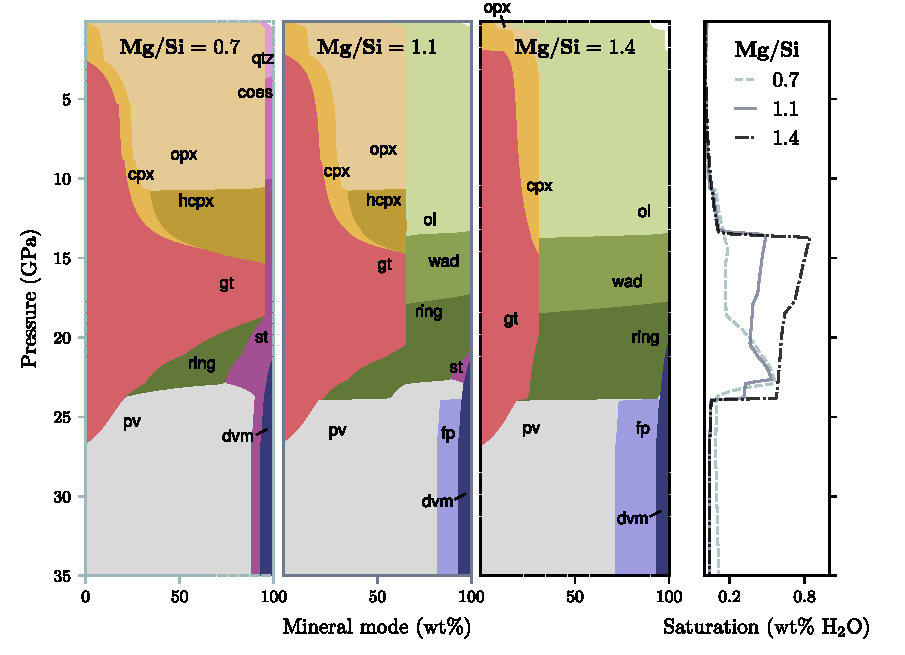
\includegraphics[width=\textwidth]{phase_demo_ver.pdf}
        \caption[Profiles of mineral mode and water saturation content, for planets with an otherwise Earth-like composition but a varying molar Mg/Si ratio.]{Profiles of mineral mode \textit{(left three panels)} and water saturation content \textit{(right panel)}, for planets with an otherwise Earth-like composition but a molar Mg/Si ratio adjusted to 1.4 \textit{(left mode panel; dashed profile)}, 1.1 \textit{(centre mode panel; solid profile)}, or 0.7 \textit{(right mode panel; dashed-dotted profile)}, respectively representing the 2nd, 50th, and 98th percentiles of exoplanet host stars in the Hypatia Catalog. Adjusted compositions are calculated conserving the total mass of MgO + SiO$_2$. Note that much of the lower mantle pressure range is not shown. Mineralogies and water saturations are for a potential temperature of 1600 K, mantle:bulk Fe of 0.113, and planet mass of $1\,M_\oplus$. Potential temperatures do not have a significant effect on the equilibrium mineralogy. For Mg/Si from 0.7 to 1.1 to 1.4, upper mantle water capacities are 0.9, 1.3 and 2.0 Earth oceans, and total mantle water capacities (i.e., including the lower mantle) are 4.7, 2.4, and 3.1 Earth oceans. Our nominal bulk silicate Earth composition is 45.0 wt.\% SiO$_2$, 37.8 wt.\% MgO, 8.05 wt.\% FeO, 4.45 wt.\% Al$_2$O$_3$, and 3.55 wt.\% CaO \citep{mcdonough_composition_1995}. Abbreviated phases are garnet (gt), clinopyroxene (cpx), orthopyroxene (opx), high-pressure clinopyroxene (hcpx),  olivine (ol), wadsleyite (wad), ringwoodite (ring), perovskite (pv), quartz (qtz), coesite (coes), stishovite (stv), ferropericlase (fp), and davemaoite (dvm).}
        \label{fig:mgsi_modality}
\end{figure*}





\section{Results}\label{sec:results-water}

\subsection{Compositionally-dependent mantle water capacities}




The modal mineralogy of a planet's mantle will depend strongly on its molar ratio of Mg to Si, the two most abundant refractory elements in the mantle. The largest variations in mineralogy, in response to changing Mg/Si, occur in the upper mantle. At Mg/Si around unity, (Mg,Fe)$_2$SiO$_4$ (ol polymorphs) and (Mg,Fe)$_2$Si$_2$O$_6$ (opx and hcpx) occur in roughly equal proportions; increasing Mg/Si favours (Mg, Fe)$_2$SiO$_4$ and decreasing Mg/Si favours opx, cpx and garnet. Below a critical value of Mg/Si ($\sim$0.8), however, no ol is stable at all, and the excess Si starts to appear as \ce{SiO2} polymorphs.

In the lower mantle, increasing Mg/Si favours (Mg,Fe)O (fp) at the expense of (Mg,Fe)SiO$_3$ (pv), and decreasing Mg/Si favours the converse. Again, \ce{SiO2} appears in appreciable quantities below a critical value of Mg/Si.

Fig. \ref{fig:mgsi_modality} illustrates the mineral mode changes and resulting water capacity profiles from simply varying Mg/Si across the typical range in our stellar sample, 0.72--1.41 (95\% of stars). At the high end of this range, the dominating wad and ring phases lead to a large capacity for water storage in the MTZ. With decreasing Mg/Si, the proportions of ol, wad, and ring diminish, and the water capacity of the MTZ correspondingly decreases as well. These overall shapes of the water saturation profile around the MTZ are robust to the details of water capacity parameterisations, given that $D^{\rm wad}_{\rm ol} \gg D^{\rm ol}_{\rm opx}$ \citep{bercovici_wholemantle_2003, dong_constraining_2021, andrault_mantle_2022}. 

% For star systems within 2$\sigma$ of average Mg/Si, we expect upper mantles with higher Mg/Si and thus more-abundant (Mg, Fe)$_2$SiO$_4$ to be wetter, up to about twofold. 

Although Fig. \ref{fig:mgsi_modality} does not show most of the lower mantle, decreasing Mg/Si also shrinks the proportion of ppv relative to pv by deepening the pv-ppv transition pressure. Given that $c_{\rm ppv} > c_{\rm pv}$ \citep[in the presence of Al;][]{townsend_water_2016}, this lower mantle effect also contributes to the decrease in overall water capacity with decreasing Mg/Si.

Upon a further decrease of Mg/Si beyond $\sim$0.8, the trend of decreasing water capacity with decreasing Mg/S starts to break. Here, \ce{SiO2} polymorphs can now form sizeable proportions of the mantle volume, in a quite un-Earth-like regime (note that allowing Si to partition into the core would diminish the occurrence rate of planets with low Mg/Si). Our model adopts $c_{\rm stv}$ comparable to wad and ring \citep{panero_hydrogen_2004, litasov_high_2007}. If stv indeed has such potential as a water reservoir, then the lower mantle's sheer volume means that even small proportions of stv (<10 wt.\%) could contribute many Earth oceans of water storage capacity. This effect is especially distinctive for larger planets, as we discuss in the next section.










% \todo{compare to \citet{andrault_mantle_2022} estimate of 0.6(0.1) OM / 2200(300) ppm wt H2O in Earth's MTZ; 0.31(0.03) OM in OBM = ~1 OM in UM. OBM water capacity in olivine-bearing mantle (OBM) of 1700(200) ppm H2O at 410 km for a mantle potential temperature of 1650 K}
% \todo{at 1650 K we get for Earth: obm 0.12 OM, mtz 1.25 OM, um 1.37 OM}

\subsection{Scaling mantle water capacity with planet mass}



\begin{figure}
    \centering
    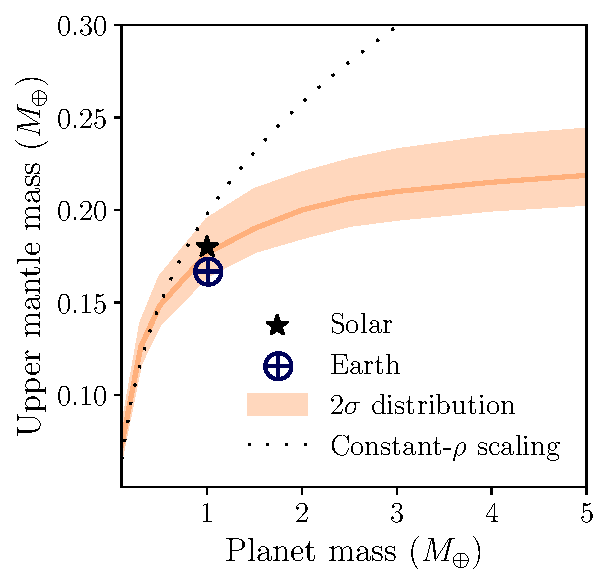
\includegraphics[width=0.6\textwidth]{pops_dist_M_p_mass_um.pdf}
    \caption[Scaling of the upper mantle mass with the total planet mass.]{Scaling of the upper mantle mass with the total planet mass. The upper mantle is defined as the shell bounded by the surface and the first occurrence of perovskite. The solid orange line shows the median upper mantle mass, and the swath spans the 2$\sigma$ distribution across compositions of planet-hosting stars from the Hypatia Catalog ($N = 1285$). Results are shown for a potential temperature of 1600 K and a mantle:bulk Fe of 0.113. Note that an FeO-free mantle would result in 5--10\% less-massive upper mantles on average, compared to those shown here; potential temperature has no effect. The $\oplus$ symbol shows the modelled result for an Earth-like bulk composition \citep{mcdonough_composition_1995}, which at $1.04 \times 10^{24}\,{\rm kg}$ is close to the observed value of $1.06 \times 10^{24}\,{\rm kg}$ \citep{nolet_earth_2011}. The star shows an Earth-mass planet with solar bulk composition; i.e., a lower Mg/Si than observed \citep{lodders_abundances_2009}. The dotted line represents a simplified scaling assuming a constant mantle density of $4500\,{\rm kg\,m^{-3}}$ and an Earth-like bulk density of $5510\,{\rm kg\,m^{-3}}$, which overestimates the upper mantle mass at large $M_p$ because compression dictates that massive planets become denser and contain proportionately more mass at depth.}
    \label{fig:mass_um}
\end{figure}


Having demonstrated how the MTZ features prominently in mantle water capacity profiles across a range of compositions, we explore the consequences of this fact on $w$-$M_p$ scaling relationships. High-water-capacity phases characteristic to the MTZ are only stable in a thin layer between about 14 and $24\,{\rm GPa}$---pressure limits which hold, with only small variation, across most planet compositions. % mantle Mg# can change this by like 1 GPa
The further, less obvious fact is that as $M_p$ increases beyond $1\,M_\oplus$, the ring-pv transition pressure does not underlay markedly more mass in the overlying upper mantle, even with the increased planet surface area (Fig. \ref{fig:mass_um}). In other words, beyond $1\,M_\oplus$, upper mantle masses become nearly independent of $M_p$ ($\propto M_p^{0.15}$ if $M_p > 1 \, M_\oplus$) %, since the upper mantle mass quickly falls below 1\% of $M_p$. %Therefore, from (\ref{eq:water_mass}), the only way to change $w_{\rm um}$ is by altering the proportions of the wettest constituent phases---e.g., by varying Mg/Si, as per the previous section. 

Note that Mars-sized ($\sim$0.1$\,M_\oplus$) planets will not be deep enough to stabilise pv. Such planets would not have bona fide lower mantles; only upper mantle phases could contribute water capacity.

% still don't know why earth has slightly lower um mass but not significant


\begin{figure*}
\centering
  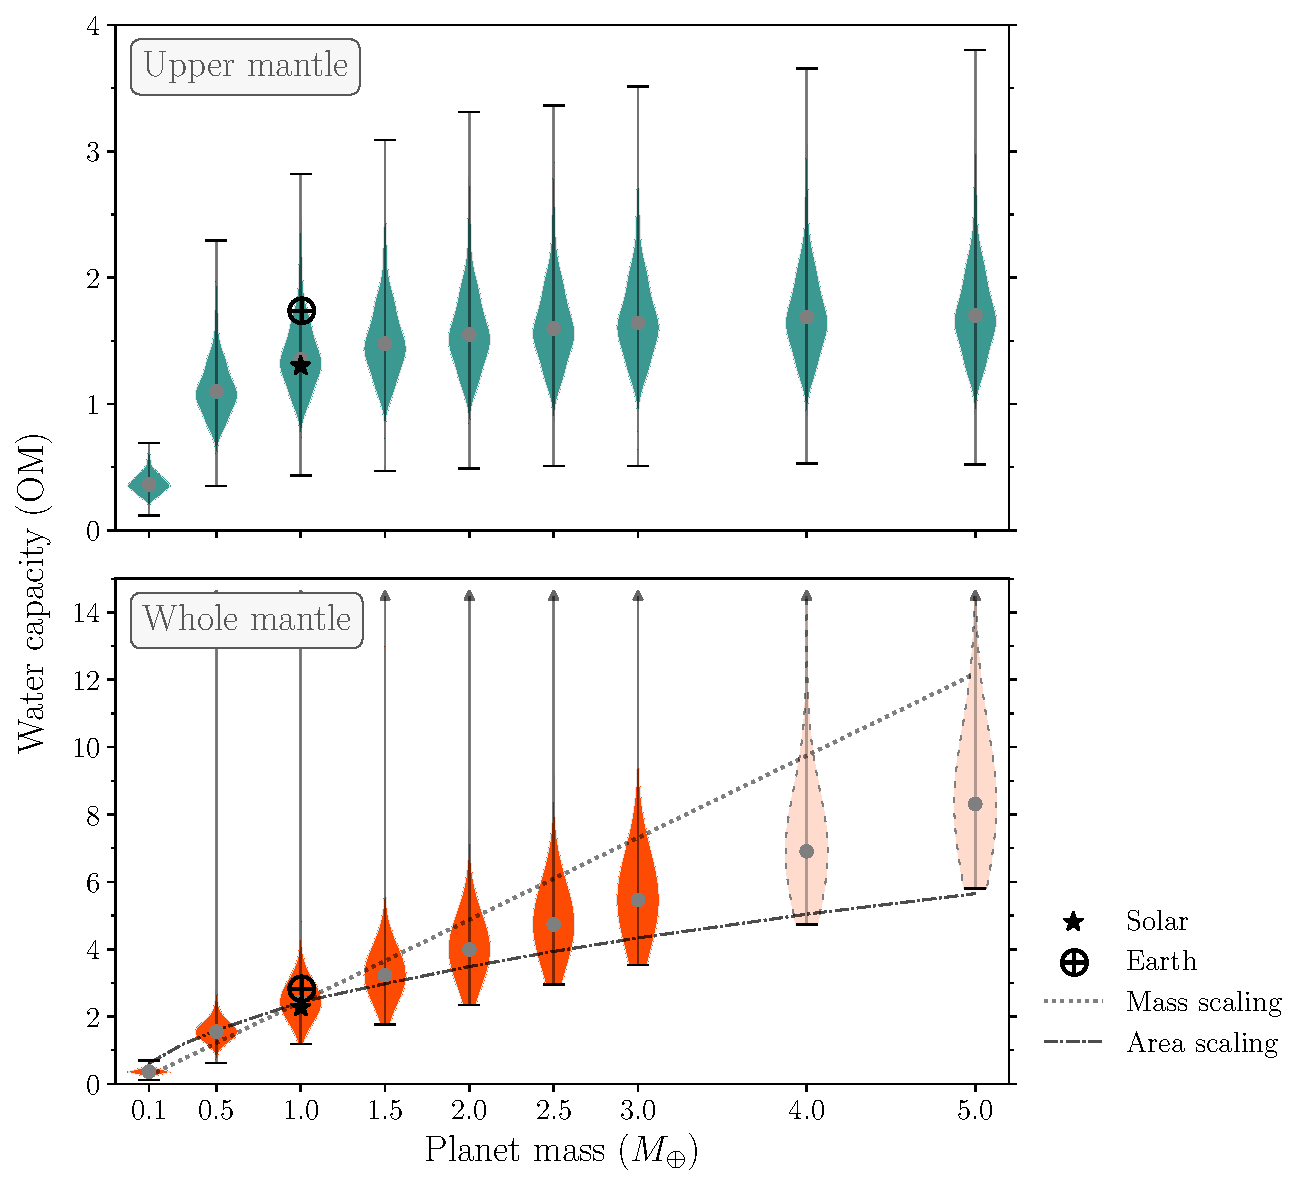
\includegraphics[width=\linewidth]{viol-Mp.pdf}
\caption[The total mass of water stored in hypothetical planetary mantles, shown as a function of planet mass.]{The water storage capacities in terms of Earth ocean masses (OM; $1\,{\rm OM} = 1.335 \times 10^{21}\, {\rm kg}$), as a function of planet mass, for the upper mantle \textit{(top)} and total mantle \textit{(bottom)}. The distributions of water capacities at each planet mass arise from the variation over the entire range of host star compositions in the Hypatia Catalog ($N = 1285$). The $\oplus$ marker shows the modelled Earth value using the bulk composition of \citet{mcdonough_composition_1995}, and the star shows a planet with solar bulk composition from \citet{lodders_abundances_2009}. The dotted line scales the 1 $M_\oplus$ median by a constant water mass fraction, $\propto (M_p / M_\oplus)$, whilst the dash-dotted line scales it with planetary surface area, $\propto (M_p / M_\oplus) (g_s/g_{s, \oplus})^{-1}$, as suggested by \citet{cowan_water_2014}. Results are shown for a potential temperature of 1600 K and a mantle:bulk Fe of 0.113. Note that for anomalously silica-rich compositions, the total mantle water capacity can reach \textgreater1\% of the planet mass, not visible in these $y$-axis limits. Dashed violin outlines indicate planet masses which result in maximum mantle pressures above the predicted recombination of MgSiO$_3$ postperovskite with MgO or SiO$_2$ \citep{umemoto_phase_2017}, which is not included in our modelling and hence these distributions are only estimates.}
\label{fig:violin_masses}
\end{figure*}



Fig. \ref{fig:violin_masses} presents the water capacity distributions we predict over chemically-diverse exoplanets as a function of their mass, shown here for an ``old and cold'' $T_p = 1600\,{\rm K}$ and an Earth-like \coreeff. As the upper mantle mass asymptotes with increasing $M_p$, so does the upper mantle water mass at water saturation---approaching a median of about 1.7 Earth ocean masses (OM; $1\,{\rm OM} = 1.335\times 10^{21}\,{\rm kg}$) at this $T_p$ (Fig. \ref{fig:violin_masses}; top panel). Mineralogical variability leads to an interquartile range of $\sim$0.4~OM for $M_p > 1\, M_\oplus$. 

Meanwhile, the water capacity of the whole mantle (Fig. \ref{fig:violin_masses}, bottom panel) necessarily increases with $M_p$. Despite the uncertainty due to poorly-constrained water saturations of lower mantle phases (see section \ref{sec:results_sensitivity}), the slope of $w_m$ with $M_p$ is credible. It falls, as expected, between a constant scaling of Earth's water capacity with $M_p$ and with planet surface area: 

\begin{enumerate}
\item The median $w_{\rm m}$ should be lower, and have a shallower slope with $M_p$, than the value implied by the scaling that treats the whole mantle as having a constant water saturation: $(w_{\rm m}/w_{\rm m, \oplus}) \propto (M_p / M_\oplus)$ (Fig. \ref{fig:violin_masses}, dotted line). This is because we know that water saturation peaks sharply at the MTZ, which represents less and less of the overall mantle mass at larger $M_p$.


% The second angle is that the mineralogy of the lower mantle is simpler than the upper mantle: phase transitions are few and far between. For any bulk composition in the set, to increase $M_p$ is to add another layer of the same minerals (i.e., mostly ppv) to the base of the mantle, with the same saturation water mass. Thus, if ppv saturation is approximately constant with pressure, then the scaling should be linear at large $M_p$. \todo{[I don't really know how to say this, and I think actually I'm making a simple thing sound too complicated and should delete this, but I guess my point is if you plot this same 1:1 mass scaling as the dotted line on figure \ref{fig:violin_masses} but with respect to an Earth composition at 5 $M_\oplus$ instead of 1 $M_\oplus$, the line goes right through the medians of 3, 4, 5 $M_\oplus$, which is the regime where approximately the whole mantle is ppv.]}
%ppv, at least, is predicted to dominate the mantle composition from roughly $\sim$120 GPa to to $\sim$450 GPa. 

\item As suggested by \citet{cowan_water_2014}, water capacity would scale in the same way as the surface area if it were focused \textit{only} into a thin shell in the upper mantle; that is, $(w_{\rm m} / w_{\rm m, \oplus}) \propto (M_p / M_\oplus) (g_s/g_{s, \oplus})^{-1}$ (Fig. \ref{fig:violin_masses}, dashed line). The true median $w_m$ should be higher than the value implied by this scaling because the rest of the mantle has nonzero water capacity. 

\end{enumerate}

Whilst the scaling in \textit{(i)} is not appropriate around 1 $M_\oplus$, $w_{\rm m}$ does indeed increase roughly linearly with $M_p$ at higher $M_p$, where the upper mantle is a less significant fraction of the whole mantle (and given our model where $c_{\rm ppv}$ is more or less constant with $P$). Between 1 and 1.5 $M_\oplus$, the integrated lower mantle water capacity first begins to outstrip $w_{\rm um}$; by 3 $M_\oplus$ the lower mantle can hold about 2.5 times the water mass of the upper mantle. 

%(the upper mantle making $\lesssim$5\% of the mantle mass at $5\,M_\oplus$). Consequentially, 

Finally, also intriguing in Fig. \ref{fig:violin_masses} is the suggestion that an Earth-like Mg/Si results in a higher interior water capacity with respect to the average Mg/Si measured in FGKM stars. Earth's mantle Mg/Si places it at the 85th percentile of $w_{\rm m}$ for planets with the same mass and Fe partitioning---this is due to larger fractions of wad and ring in Earth's MTZ than is typically predicted for planets. However, as discussed in section \ref{sec:discussion-sio2-water}, the Mg/Si abundances of stars may be lower than the composition of their associated rocky planet mantles if some fraction of a planet's inherited bulk Si were commonly locked in the metal core during formation. Indeed, the raw solar Mg/Si is actually slightly below the stellar average in Hypatia; a planet with Si-Mg-Fe-Ca-Al composition at exactly the solar value and an Earth-like core fraction would have $w_{\rm m}$ at the 31st percentile.




Evaluating our parameterisation for an Earth-like composition gives an MTZ water capacity of 1.25 OM and an olivine-bearing mantle water capacity of 0.12 OM, if we use the same potential temperature ($T_p = 1650\,{\rm K}$) as \citet{andrault_mantle_2022}---corresponding to a wetter MTZ and drier olivine-bearing mantle compared to that work, which finds 0.6 OM and 0.31 OM, respectively, and a drier upper mantle overall.
% 1.37 vs. 0.91



\subsection{Interior water mass fractions of rocky planets}




\begin{figure*}
    \centering
    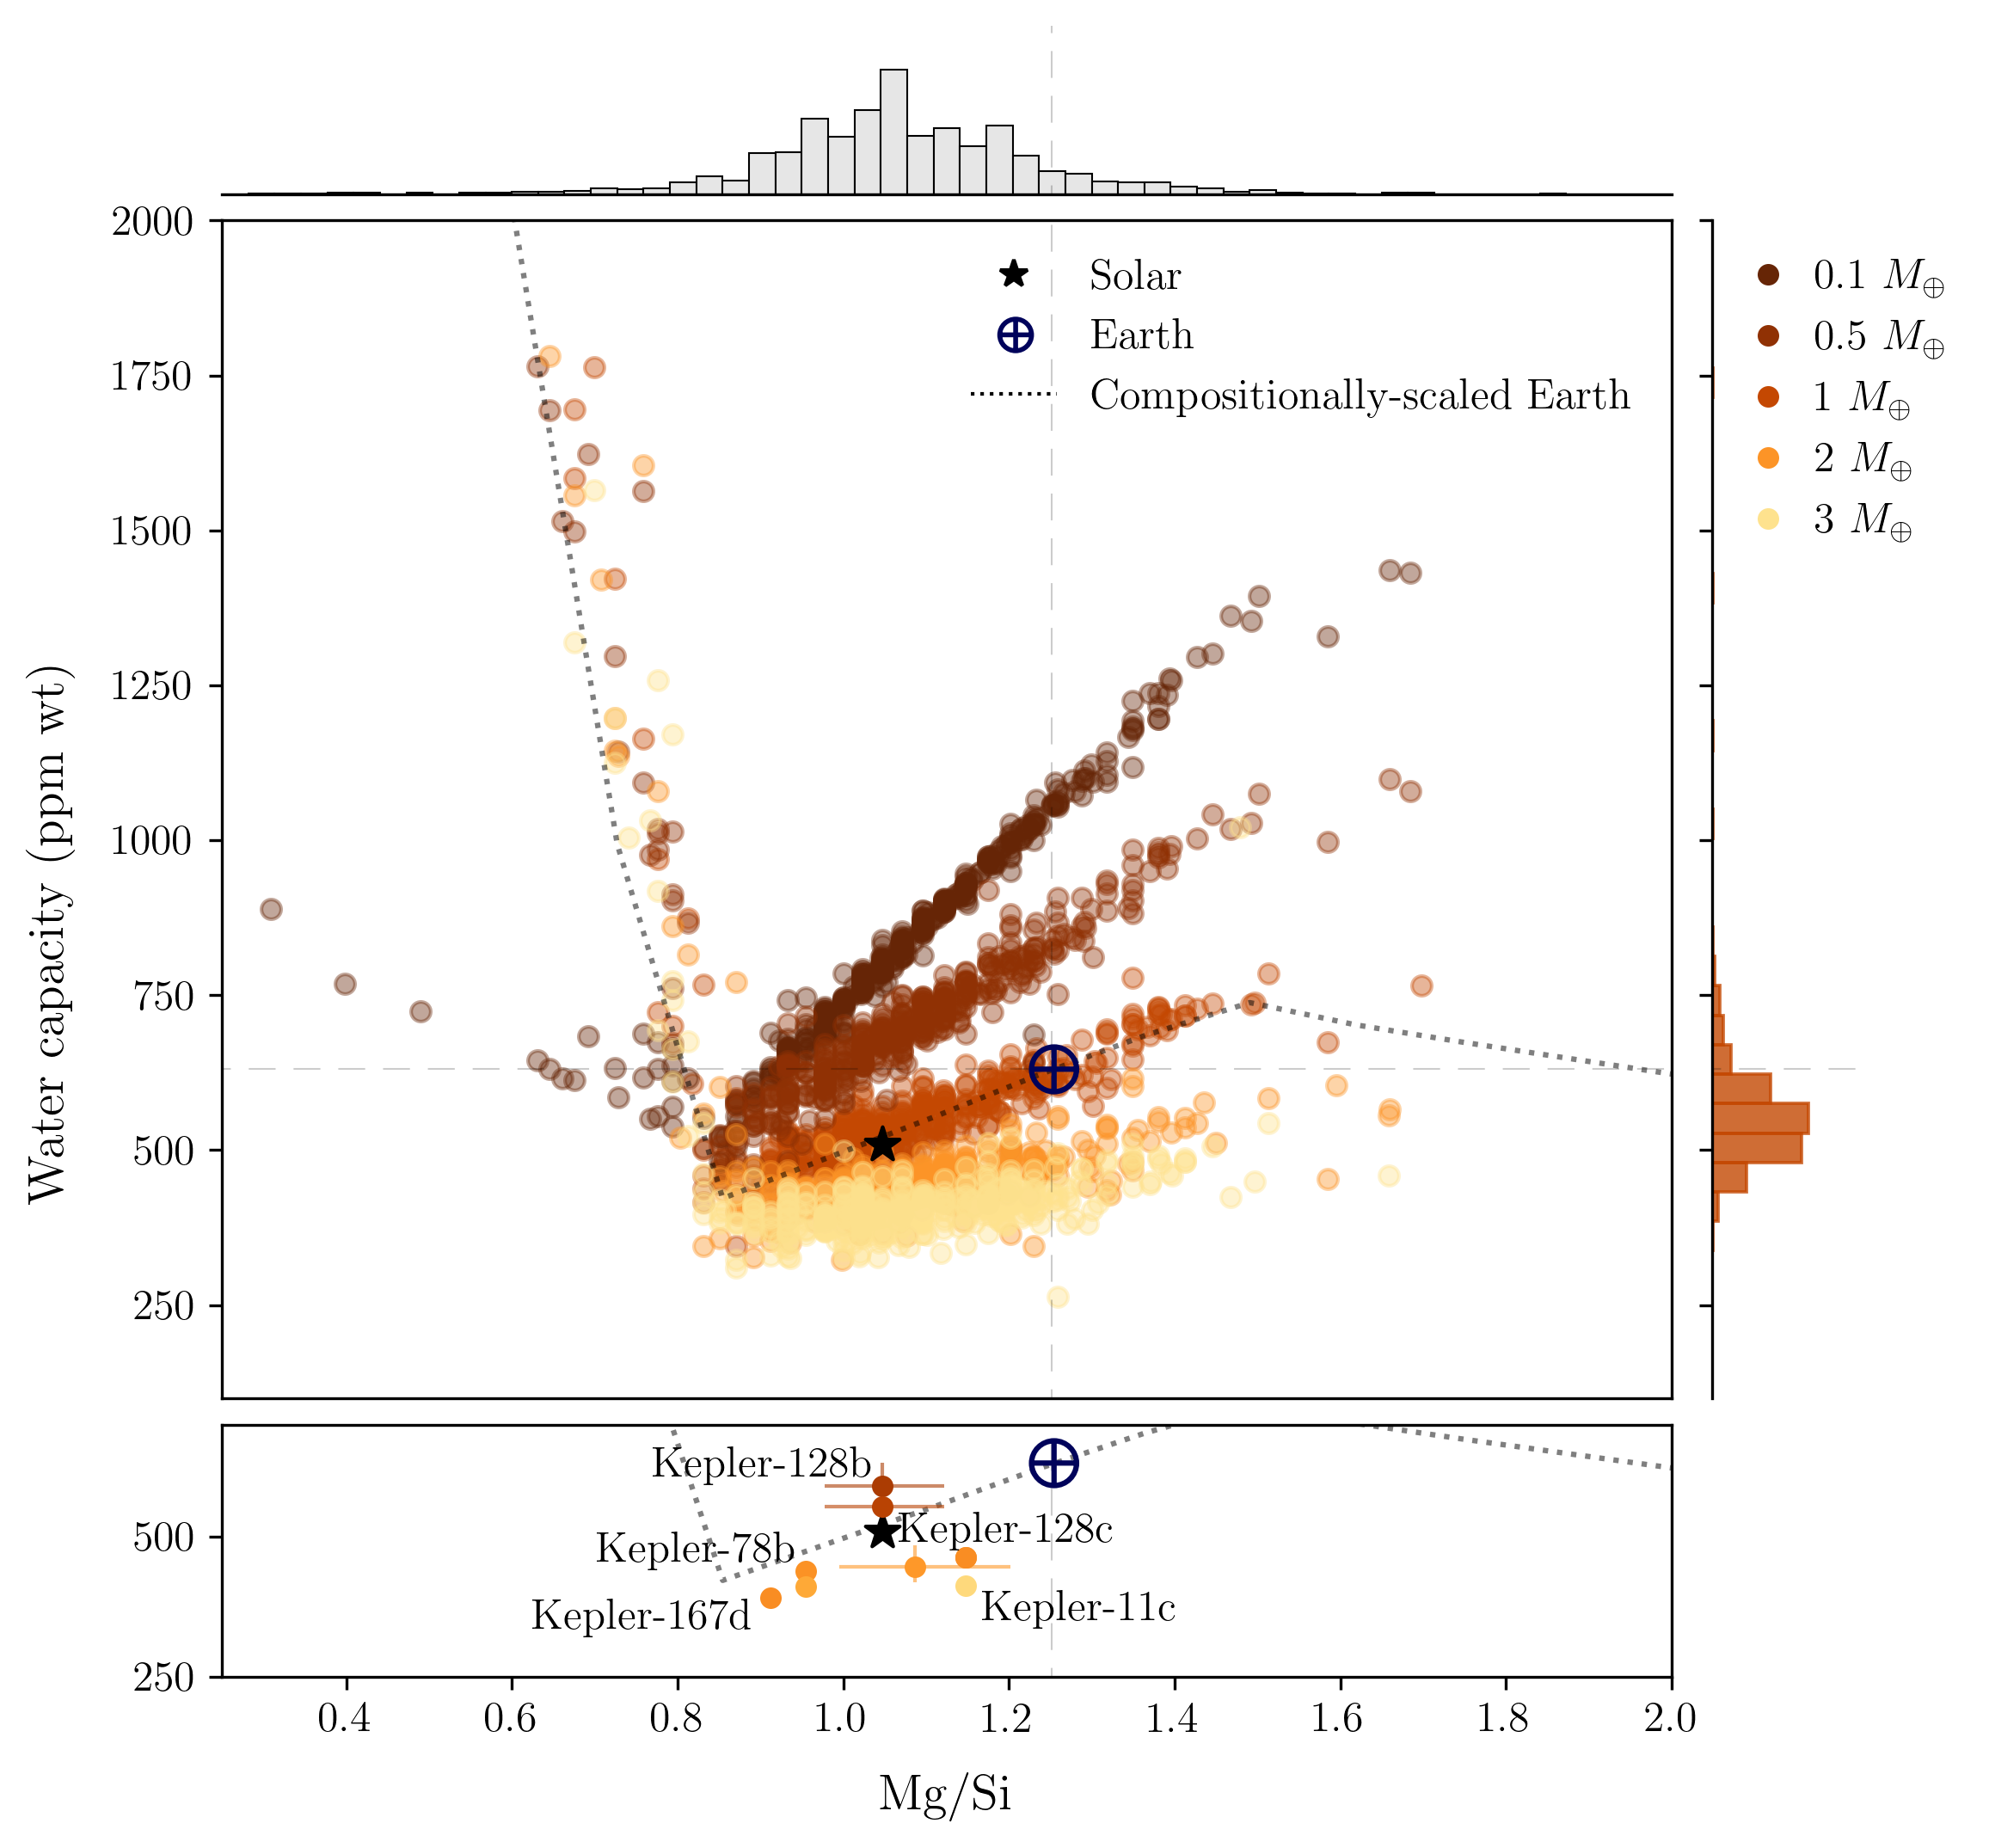
\includegraphics[width=\textwidth]{mgsi_c_h2o_exo_r2.png}
    \caption[Water storage capacities, expressed as a mass fraction with respect to the total planet mass, of hypothetical planets having the compositions of planet-hosting stars from the Hypatia Catalog.]{\textit{(Top:)} Interior water storage capacities, expressed as a mass fraction with respect to the total planet mass, of hypothetical planets having the compositions of planet-hosting stars from the Hypatia Catalog. Results are shown as a function of the Mg/Si ratio, which is the key compositional variable controlling mantle water storage capacity. Colours represent the planet mass; $2\,M_\oplus$ and $3\,M_\oplus$ planets nearly overlap. \textit{(Bottom:)} The same as above, but focused in on a selection of confirmed exoplanets using their host star compositions and median mass measurements from Hypatia (errors are propagated from the minimum and maximum stellar Mg/Si reported where multiple measurements exist). Models assume mantles with a potential temperature of 1600 K and a mantle:bulk Fe ratio of 0.113. The round symbol represents the modelled Earth value, and the dotted line represents variable Mg/Si with an otherwise Earth-like composition \citep{mcdonough_composition_1995}. The star symbol shows a planet with solar bulk composition \citep{lodders_abundances_2009}. The distributions of Mg/Si and water capacities are projected as histograms on the top and right (for $1\,M_\oplus$) axes, respectively. Note that the $y$-axis limit on water capacity crops the highest water storage capacities at the extreme low end of Mg/Si (water capacities $> 10,000$ ppm), and the $x$-axis limit on Mg/Si excludes two stars with ${\rm Mg/Si }>2$.}
    \label{fig:h2o_mgsi_scatter}
\end{figure*}



Fig. \ref{fig:h2o_mgsi_scatter} shows these same interior water capacities not as an absolute water mass, but as a mass fraction of water with respect to $M_p$. Although more massive planets can clearly sequester more water, these water masses corresponds to much lower fractions of the overall planet mass. A planet with Earth's bulk composition has a mantle water capacity of $\sim$1000~ppm at 0.1 $M_\oplus$, but the mantle of a $3\,M_\oplus$ planet of the same composition can only contain $\sim$400~ppm. The corollary of this is that if these two planets accreted the same mass fractional water budget, the larger planet would be able to store less of this water in its mantle. This point carries notable implications for the frequency of ocean-covered planets and is discussed in section \ref{sec:discussion-waterworld}.  %Given a nearly pressure- and temperature-independent $c_{\rm ppv}$, water capacity mass fractions stay roughly constant as soon as ppv comprises the majority of the mantle by mass. 

There is a water capacity trend with bulk composition at all planet masses. In the typical range of stellar Mg/Si, water capacity increases with increasing Mg/Si because more wad and ring are stabilised at the expense of gt in the MTZ region (Fig. \ref{fig:mgsi_modality}). The slope of water capacity with Mg/Si flattens at higher $M_p$ because the contribution of the $\sim$14--24-GPa MTZ becomes less important than the lower mantle. That is, the water capacities of pv, ppv, and fp are similar, so their changing proportions due to changes in bulk composition have little effect on lower mantle water storage capacity.

To highlight the compositional dependence of mantle water storage capacity, we also isolate the effect of changing Mg/Si on its own for an otherwise Earth-like bulk composition (Fig. \ref{fig:h2o_mgsi_scatter}, black dotted line). Again, there is an evident increase in water capacity around the Mg/Si range near Earth's bulk composition. However, we see two kinks around the extrema of Mg/Si $\lesssim 0.8$ and Mg/Si $\gtrsim 1.5$, where key changes in the modal mineralogy occur. In the former shift---the extreme low end---all Mg has been used in forming pyroxenes, and excess Si is left as the silica polymorphs qtz, coes, stv, and seif. Silica-rich mantles can attain very high water contents, due to the high water capacity of stv we adopt here (section \ref{sec:methods_sat}). Mars-sized (0.1 $M_\oplus$) planets do not have deep-enough mantles to host significant masses of stv, so the associated water capacity increase at low Mg/Si is only moderate. Meanwhile, for Mg/Si $\gtrsim1.5$, there is excess Mg beyond that which is incorporated into wad and ring, so dry fp appears even in the MTZ.

For illustration, Fig. \ref{fig:h2o_mgsi_scatter} also shows our calculated interior water mass fractions for a selection of known exoplanets, given their mass and host star composition measurements. %(The climates on these planets will not necessarily stabilise surface liquid water.)


\subsubsection{Sensitivity to water saturation parameterisation}\label{sec:results_sensitivity}
A large part of the uncertainty on the interior water capacities of planets near $1\,M_\oplus$ comes from the unknown water storage of pv. \citet{dong_constraining_2021} tested the sensitivity of an Earth-mass, Earth-composition mantle water capacity to  $D^{\rm ring}_{\rm pv} \in [7, 23]$ \citep{inoue_water_2010}, and simultaneously to the regression uncertainty on their fit parameters, finding 25th- and 75th- percentile water capacities at around $\sim$10--20\% away from the 50th percentile value. Predictions of mantle water capacities for any bigger planet would be more uncertain, predominantly because the water capacity of postperovskite, and its pressure dependence, are so poorly constrained. Postperovskite could reasonably hold more water with increasing pressure---as does olivine and stishovite \citep{panero_hydrogen_2004, dong_constraining_2021}---in which case massive planets would be effective at sequestering deep water. Nevertheless, these deep mantle water reservoirs might not be communicating efficiently with the planetary surface, especially if a low $c_{\rm pv}$ at the top of the lower mantle creates a bottleneck to water circulation (see section \ref{sec:discussion-dynamics}).
%At $1\,M_\oplus$, the lowermost mantle already stabilises ppv, so at higher $M_p$ the total volume of pv would not increase greatly. If we believe that ppv holds $\sim$2--4$\times$ more water than pv \citep{townsend_water_2016} a similar sensitivity analysis at higher $M_p$ would result in slightly higher uncertainties compared to \citep{dong_constraining_2021}.



\subsection{Mineralogical and structural effects of planetary Fe partitioning}\label{sec:results_fe}



\begin{figure}
    \centering
    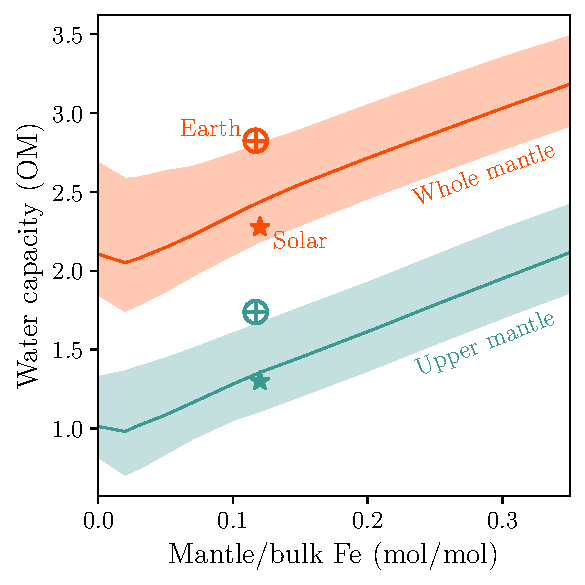
\includegraphics[width=0.6\textwidth]{x_Fe_dependence.pdf}
    \caption[The dependence of mantle water storage capacity on the extent of core formation.]{Total mantle (red) and upper mantle (blue) water capacities, in Earth ocean masses (OM), as a function of the molar fraction of mantle Fe to bulk Fe. Solid lines follow medians and swaths span the 1$\sigma$ distributions across compositions of planet-hosting stars from the Hypatia Catalog. Results are shown for a potential temperature of 1600 K and a planet mass of $1\,M_\oplus$. The round symbol represents the modelled Earth value using its measured composition \citep{mcdonough_composition_1995}, and the star symbol is for a planet with solar bulk composition \citep{lodders_abundances_2009}.}
    \label{fig:x_Fe_dependence}
\end{figure}




So far, we have shown results for planets with constant \coreeff. Changing how Fe is partitioned between the mantle and the core of a planet has several distinct effects on the interior water capacity (see Supplementary Figs. \ref{fig:wmf_scatter}--\ref{fig:pressure_gradients_feh}):

\begin{enumerate}
    \item A more massive core (with a resultant lower CMB pressure) will shift the entire mass profile of the mantle upwards, and steepen the pressure gradient, with the consequence of less mass underlying the ring-pv transition, and a lower UM mass \citep{unterborn_scaling_2016, unterborn_pressure_2019}.
    \item A more FeO-rich mantle will also have a steeper pressure gradient.
    \item A more FeO-rich mantle will have a higher water concentration at saturation, all else equal, because this composition favours olivine polymorphs over gt in the UM, produces a shallower ol-wad transition in the UM, and produces a shallower pv-ppv transition in the LM.
\end{enumerate}

If we move iron from the core to the mantle (as FeO), the net effect is a slightly higher UM mass, and a higher average water saturation in ppm wt for both the UM and LM. These effects amplify each other to result in a larger water capacity at larger \coreeff~(Figure \ref{fig:x_Fe_dependence}).

The other way to change CMF and mantle FeO content in our model, which conserves $M_p$ and bulk composition, is to have a more Fe-rich star: extra iron everywhere raises both the CMF and the mantle FeO content. In contrast to changing \coreeff, these two effects have competing consequences for water capacities---a lower UM mass but a higher water saturation---with the net effect being a slight decrease (more so at higher $M_p$). 

A corollary of the results described above is that mantle water capacities depend more strongly on the Mg/Si ratio than on the Fe/Si ratio of the system. This analysis does not account for possible direct effects of Fe on mineral water saturation, which, except for olivine, are not easily resolvable with the current experimental data \citep{dong_water_2022}.


% \todo{START HERE NEXT}

% In our model, preserving the planet mass and bulk Fe content, we can alter mantle FeO content in two ways: increase \coreeff~with constant bulk planet Fe, or increase bulk Fe (i.e., a more Fe-rich star) without allowing the distribution of Fe between FeO and Fe-metal to change. In either scenario, the higher mantle FeO favours ol polymorphs over gt in the MTZ, and also stabilises wad $\lesssim 1\,{\rm GPa}$ closer to the surface \citep{katsura_olivine-wadsleyite_2004}. Both these effects result in larger upper mantle water capacities. Increasing \textit{bulk} planet Fe/Mg also promotes thinner ppv layers as the core mass increases and the core-mantle boundary extends to lower pressure. The opposite is true if mantle FeO is increased at the core's expense. The net effect of these considerations is that total water capacity decreases slightly with the bulk Fe content of the planet. 

% Fig. \ref{fig:x_Fe_dependence} shows how varying \coreeff~affects $m_w$ over the Hypatia sample: oxidising 30 mol\% of the planet's Fe will raise $m_w$ by 30\% on average. This effect is primarily due to changes in the mineralogy induced by mantle FeO content. Across-star variations in bulk Fe manifest as scatter in Fig. \ref{fig:h2o_mgsi_scatter}. Overall, mantle water capacities correlate significantly more strongly with bulk Mg/Si than with bulk Fe/Si.





% \todo{[Should we bother plotting $\Delta w_{\rm m}$ as a function of $M_p$ and/or Mg\#?]}




% \todo{especially garnet, Ca-pv, SiO2 polymorphs - if you change their saturation by 2 or 10, for example, what happens to the interior water capacity? \citet{dong_constraining_2021} already covered this especially with bridgmanite uncertainty, I won't be as serious as their MCMC method, if I do anything. planning to do these just at 1 mass, Tp, \coreeff. NB just need to rerun saturation module (faster), not solve interior structure and mineralogy again.}

\subsection{Results summary}

Table \ref{tab:all_results} lists our results for the upper and total mantle water capacity distributions as a function of $M_p$, $T_p$, and \coreeff. Although the results presented so far have focused on an old and cold scenario of $T_p = 1600\,{\rm K}$, we have suggested that the hot temperature profile, realised immediately after magma ocean crystallisation, is the relevant temperature that locks in the water content of the interior---at which the solid seals itself from the overlying water (see section \ref{sec:discussion-temperature}). Hence Table \ref{tab:all_results} also reports results at $T_p = 1900\,{\rm K}$.

% \todo{Here put other table listing main effects?}


\begin{table*}
\centering
\caption[Medians and 2$\sigma$ widths of the distribution of exoplanet mantle water capacities inferred from stellar compositions in the Hypatia Catalog.]{Mantle water capacity medians across stellar compositions from the Hypatia Catalog, and 2$\sigma$ widths in parentheses, as a function of planet mass ($M_p$), potential temperature ($T_p$), and molar mantle:bulk iron ratio (\coreeff). $1\,{\rm OM} = 1.335 \times 10^{21}\,{\rm kg}$. \label{tab:all_results}}
\footnotesize


\begin{tabular}{@{} c c l l l l l @{}}
\toprule
& & \multicolumn{5}{c}{\coreeff} \\ \cmidrule(lr){3-7}
$T_p\,{\rm (K)}$ & $M_p\,(M_\oplus)$ & 0.30 & 0.20 & 0.12 & 0.05 & 0.00 \\
\midrule
\noalign{\vskip 1mm}
%%%%%%%%%%%%%%%%%%%%%%%%%%%
% start copy




\multicolumn{7}{c}{\textbf{Whole mantle water capacity (OM)}} \\
\multirow{10}{*}{1600} & 0.1 & 0.60 (0.40) & 0.47 (0.35) & 0.37 (0.32) & 0.29 (0.30) & 0.24 (0.29) \\
 & 0.3 & 1.53 (0.89) & 1.30 (0.94) & 1.11 (0.96) & 0.92 (1.04) & 0.82 (1.16) \\
 & 0.5 & 2.05 (1.14) & 1.79 (1.37) & 1.56 (2.01) & 1.33 (2.77) & 1.29 (3.14) \\
 & 1.0 & 3.03 (1.61) & 2.71 (3.01) & 2.44 (5.16) & 2.15 (7.14) & 2.11 (8.05) \\
 & 1.5 & 3.87 (1.97) & 3.53 (4.41) & 3.23 (7.35) & 2.92 (10.24) & 2.86 (11.49) \\
 & 2.0 & 4.66 (2.27) & 4.30 (5.83) & 3.99 (9.44) & 3.66 (12.98) & 3.61 (14.48) \\
 & 2.5 & 5.40 (2.61) & 5.04 (7.23) & 4.73 (11.47) & 4.41 (15.61) & 4.34 (17.29) \\
 & 3.0 & 6.13 (3.00) & 5.78 (8.63) & 5.47 (13.43) & 5.13 (18.09) & 5.06 (19.86) \\
 & 4.0 & 7.56 (3.80) & 7.22 (11.36) & 6.90 (17.25) & 6.57 (23.02) & 6.50 (25.22) \\
 & 5.0 & 8.96 (4.95) & 8.62 (13.90) & 8.31 (21.04) & 7.99 (27.81) & 7.91 (29.88) \\
\hline
\multirow{10}{*}{1900} & 0.1 & 0.17 (0.11) & 0.13 (0.10) & 0.11 (0.11) & 0.09 (0.12) & 0.09 (0.14) \\
 & 0.3 & 0.54 (0.31) & 0.48 (0.85) & 0.43 (1.35) & 0.39 (1.75) & 0.39 (2.31) \\
 & 0.5 & 0.83 (0.54) & 0.76 (1.89) & 0.70 (3.12) & 0.66 (4.32) & 0.65 (5.57) \\
 & 1.0 & 1.50 (1.07) & 1.41 (4.13) & 1.35 (7.05) & 1.30 (9.67) & 1.29 (11.18) \\
 & 1.5 & 2.16 (1.61) & 2.08 (5.69) & 2.01 (9.44) & 1.96 (13.25) & 1.95 (15.02) \\
 & 2.0 & 2.82 (2.11) & 2.74 (7.12) & 2.67 (11.68) & 2.63 (16.30) & 2.62 (18.40) \\
 & 2.5 & 3.48 (2.60) & 3.40 (8.51) & 3.34 (13.79) & 3.29 (19.06) & 3.28 (21.71) \\
 & 3.0 & 4.14 (3.10) & 4.07 (9.88) & 4.01 (15.87) & 3.96 (21.63) & 3.95 (24.56) \\
 & 4.0 & 5.47 (4.10) & 5.40 (12.55) & 5.34 (19.75) & 5.30 (26.66) & 5.30 (29.59) \\
 & 5.0 & 6.79 (5.08) & 6.40 (35.00) & 6.68 (23.53) & 6.64 (31.35) & 6.65 (34.84) \\
\hline
\multicolumn{7}{c}{\textbf{Upper mantle water capacity (OM)}} \\
\multirow{10}{*}{1600} & 0.1 & 0.58 (0.41) & 0.46 (0.35) & 0.36 (0.32) & 0.28 (0.30) & 0.24 (0.29) \\
 & 0.3 & 1.30 (0.91) & 1.07 (0.87) & 0.89 (0.82) & 0.71 (0.81) & 0.61 (0.84) \\
 & 0.5 & 1.60 (1.11) & 1.32 (1.07) & 1.10 (1.01) & 0.88 (1.02) & 0.82 (0.95) \\
 & 1.0 & 1.95 (1.37) & 1.62 (1.33) & 1.36 (1.26) & 1.09 (1.27) & 1.01 (1.19) \\
 & 1.5 & 2.12 (1.49) & 1.76 (1.44) & 1.48 (1.36) & 1.19 (1.39) & 1.11 (1.28) \\
 & 2.0 & 2.22 (1.57) & 1.85 (1.52) & 1.55 (1.45) & 1.25 (1.45) & 1.17 (1.38) \\
 & 2.5 & 2.28 (1.61) & 1.90 (1.56) & 1.60 (1.48) & 1.29 (1.50) & 1.22 (1.41) \\
 & 3.0 & 2.35 (1.65) & 1.95 (1.61) & 1.64 (1.51) & 1.33 (1.56) & 1.25 (1.45) \\
 & 4.0 & 2.40 (1.70) & 1.99 (1.65) & 1.69 (1.56) & 1.36 (1.58) & 1.28 (1.49) \\
 & 5.0 & 2.41 (1.70) & 2.01 (1.66) & 1.70 (1.60) & 1.38 (1.61) & 1.29 (1.50) \\
\hline
\multirow{10}{*}{1900} & 0.1 & 0.16 (0.11) & 0.13 (0.10) & 0.11 (0.11) & 0.09 (0.12) & 0.09 (0.14) \\
 & 0.3 & 0.37 (0.27) & 0.31 (0.27) & 0.26 (0.27) & 0.23 (0.32) & 0.22 (0.37) \\
 & 0.5 & 0.46 (0.33) & 0.38 (0.34) & 0.33 (0.34) & 0.29 (0.40) & 0.27 (0.45) \\
 & 1.0 & 0.56 (0.41) & 0.47 (0.42) & 0.40 (0.42) & 0.36 (0.49) & 0.33 (0.54) \\
 & 1.5 & 0.61 (0.45) & 0.51 (0.46) & 0.44 (0.46) & 0.39 (0.53) & 0.36 (0.57) \\
 & 2.0 & 0.64 (0.47) & 0.53 (0.48) & 0.46 (0.48) & 0.41 (0.57) & 0.38 (0.63) \\
 & 2.5 & 0.66 (0.48) & 0.55 (0.49) & 0.48 (0.49) & 0.42 (0.59) & 0.39 (0.62) \\
 & 3.0 & 0.67 (0.51) & 0.57 (0.51) & 0.49 (0.52) & 0.43 (0.58) & 0.40 (0.65) \\
 & 4.0 & 0.68 (0.51) & 0.58 (0.52) & 0.50 (0.53) & 0.44 (0.61) & 0.40 (0.65) \\
 & 5.0 & 0.69 (0.51) & 0.65 (0.63) & 0.51 (0.54) & 0.45 (0.61) & 0.41 (0.70) \\
\hline




%%%%%%%%%%%%%%%%%%%%%%%%%%%
% end copy



\end{tabular}
\end{table*}






\section{Discussion}\label{sec:discussion-water}

\subsection{Implications and consequences}

\subsubsection{The occurrence rate of ocean planets}\label{sec:discussion-waterworld}

A key question motivating this work is how water partitions between a planet's interior and surface. This partitioning determines whether planets become fully-inundated ocean planets, or can maintain some fraction of exposed land. We have focused on one specific process out of many that feed into a planet's interior-surface water partitioning: the ability of mantle minerals to store any water with which the planet is endowed during its formation. We have shown that higher-mass rocky planets can sequester proportionally less water in their interiors, down to $\sim$300--400 ppm of the planet mass at $M_p \gtrsim 3\,M_\oplus$.


A detailed understanding of ocean planet propensity must unite all processes that govern interior-surface water partitioning. Ultimately, whether or not planets have dry land depends on the interplay of \textit{(i)} total water budgets, \textit{(ii)} water redistribution between interior and surface reservoirs, and \textit{(iii)} the theoretical capacities of these surface (i.e., ocean basin volume) and interior reservoirs. 

Estimating the initial water budget of a planet \textit{(i)} requires knowing the amount of water in planetary building blocks and the ability of the growing planet to ingas nebular hydrogen. These variables depend in turn on the planetary formation time- and space-scales, as well as on $M_p$ \citep[and references therein]{sharp_nebular_2017, unterborn_inward_2018, kimura_formation_2020, ohtani_hydration_2021}. Planetary accretion simulations, although stochastic, produce rocky planets in the classical habitable zone commonly forming with $\gtrsim$10 OM water \citep{raymond_making_2004, raymond_highresolution_2006, zain_planetary_2018}. The oxidation of ingassed nebular H could alone contribute $\gtrsim$1000~ppm water, without needing to capture icy planetesimals, depending on the stellar mass and nebular lifetime \citep{olson_nebular_2019, kimura_predicted_2022}. The water contents of enstatite, ordinary, and carbonaceous chondrites (\textgreater 1000--10,000~ppm), materials thought to sample planetary building blocks, easily exceed the mantle water capacities of Earth-mass planets and above \citep{abe_water_2000}. Note that late delivery of water by comets is not expected to contribute a significant amount of water, at least in the solar system \citep{morbidelli_source_2000}. Overall, it appears quite possible for planets to accrete water beyond that which their mantles can hold.



Estimating water redistribution \textit{(ii)} is more tractable in the stagnant lid regime. Here, with no mantle return flux, redistribution is controlled by volcanic outgassing and is tied to the thermal history of the planet \citep[e.g.,][]{ortenzi_mantle_2020}. The persistence of early oceans extruded from a cooled magma ocean is also strongly coupled with the planetary climate \citep[e.g.,][]{elkins-tanton_formation_2011, miyazaki_wet_2022}. 

Constraints on the interior reservoir capacity \textit{(iii)} are covered in this work. The potential size of the \textit{surface} reservoir depends on topography, as was shown in \citet{guimond_blue_2022}, who found that more massive planets are virtually topographically featureless and able to be flooded by a relatively smaller ocean volume.

Based our prediction of maximum mantle water mass fractions decreasing roughly as $M_p^{-0.23}$, and our previous work finding the maximum surface water mass fraction (based on the bare-minimum topography) to decrease as $M_p^{-0.75}$ \citep{guimond_blue_2022}, we speculate that land and oceans are less likely to coexist on massive rocky planets. At the end of the magma ocean stage, any water in excess of their limited solid mantle water capacities would immediately contribute to deep oceans (or thick steam atmospheres)---or, if this non-sequestered water escapes under high stellar irradiation, the planets are irreversibly desiccated. This speculation is tied to the low water capacity of pv and ppv adopted here, and would need to be re-evaluated if, for example, future experiments suggest that these deep mantle silicates can store significantly more water at higher pressures.

% cite Kimura & Ikoda paper on desiccating Earth mass planets around M-dwarfs?




\subsubsection{Consequences and corollaries of a temperature dependence of mantle water storage capacity}
\label{sec:discussion-temperature}


\begin{figure}
    \centering
    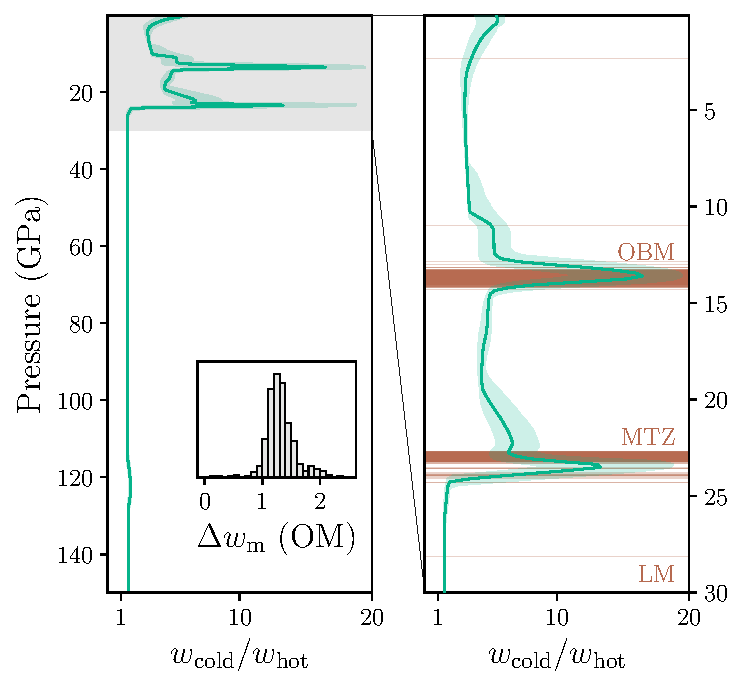
\includegraphics[width=0.8\textwidth]{sat_T_diff.pdf}
    \caption[The temperature dependence of mantle water storage capacity.]{The temperature dependence of mantle water storage capacity. Mass ratios of mantle water capacities ($w_{\rm cold}/w_{\rm hot}$) for mantles with potential temperatures of $1600\,{\rm K}$ and $1900\,{\rm K}$ are shown in two profiles, for the whole mantle \textit{(left)} and in detail to the top of the lower mantle \textit{(right)}. The swath spans the 1$\sigma$ distribution across compositions of planet-hosting stars from the Hypatia Catalog; the solid blue line shows the median. As the mantle cools, the water capacity increases for all compositions shown. Horizontal lines show the first appearances of wadsleyite and of perovskite with increasing pressure, demarcating the respective mantle regions: olivine-bearing mantle (OBM), mantle transition zone (MTZ), and lower mantle (LM). The largest values of $w_{\rm cold}/w_{\rm hot}$ are around these phase transitions, which shift $<1\,{\rm GPa}$ between the two $T_p$. This profile pertains to a $1\,M_\oplus$ planet. \textit{(Inset:)} Distribution of the difference in the whole mantle water storage capacity, in Earth ocean masses (OM), between mantle potential temperatures of $1600\,{\rm K}$ and $1900\,{\rm K}$. Not shown in the histogram axis limits are the results for anomalously silica-rich planets, the water storage capacities of which may increase with temperature.}
    \label{fig:sat_diff_T}
\end{figure}



As the mantle cools, we expect NAMs to hold more water at saturation \citep{keppler_thermodynamics_2006}---only stishovite behaves conversely in our parameterisation. For a closed system (e.g., the mantle of a stagnant lid planet undergoing no water recycling to its interior), however, the mantle water content cannot increase as the system cools, even if the minerals could in principle hold more water. We nonetheless explore the effect of temperature on the \textit{theoretical} maximum water storage capacity of planets, as this will be relevant for \textit{(i)} planets with an active surface-mantle water cycle (e.g., plate tectonic planets), and \textit{(ii)} showing how the temperature at the end of magma ocean solidification may set the mantle's initial water capacity.

We find that as a $1\,M_\oplus$ planet secularly cools by $300\,{\rm K}$ over time \citep[an amount by which Earth's own mantle may have cooled over its history;][]{HERZBERG2010}, its capacity to store water will increase by $\sim$1--2 OM (Fig. \ref{fig:sat_diff_T}), as highlighted elsewhere \citep{shah_internal_2021, dong_constraining_2021, andrault_mantle_2022}. At the present time, we cannot rectify any temperature dependence of water saturation in pv or ppv with the available data. Theoretical calculations by \citet{hernandez_incorporation_2013} find $D^{\rm ring}_{\rm pv}$ decreasing with temperature, which would mute any $T$-dependence of $c_{\rm pv}$ given that $c_{\rm ring}$ is also lower at high $T$.

The direct thermodynamic effect of cooling on water capacity is mildly stronger than the effect of variations in upper mantle mineralogy: in Fig. \ref{fig:sat_diff_T} the median ratio $w_{\rm cold}/w_{\rm hot}$ surpasses the width of the distribution of mantle water storage capacity from predicted mantle mineralogies (cf. Fig. \ref{fig:violin_masses}). Note, however, that the largest ratios ($w_{\rm cold}/w_{\rm hot}>10$) are seen around the ol-wad transition and the ring-pv transitions. Here, higher $T_p$ shifts the pressures of these transitions deeper by $\lesssim1\,{\rm GPa}$. Much higher water capacities in wad and ring effectively create a large $w_{\rm cold}/w_{\rm hot}$ ratio around these pressures.
% peak is below MTZ because of more gradual transition to pv (LM defined at top of pv)
% note little blip at 150 GPa is the cooler T raising the depth of the pv-ppv transition - also means D_ppv_brg is higher so c_ppv is higher
\medskip





Although the fact that temperature exerts a first-order control on mineral water saturation should elicit caution, we can leverage certain deterministic consequences of the thermal evolution of planets to apply our results further.

% Yet more information could be obtained, in principle, to tailor either endmember scenario for a given planet.

% We have isolated two endmember scenarios which nominally represent planets at contrasting stages of evolution: $T_p = 1900\,{\rm K}$, typifying a young planet's water storage capacity at the point of magma ocean solidification ($1900\,{\rm K}$ approximating the shallow solidus temperature of peridotite); and $T_p = 1600\,{\rm K}$, the temperature of a planetary mantle after secular cooling, roughly Earth's modern mantle temperature.


\paragraph{Patterns in $T_p$ across planets}

The mantle temperatures of a planet at thermal quasi-steady state relate predictably to its mass and tectonic mode. Whilst a $T_p$ of $\sim$1600$\,{\rm K}$ is appropriate for an Earth-mass planet in a plate tectonic regime, more massive planets will run hotter.
% , given some assumptions about the planet's rheology, radiogenic element abundance, and tectonic mode. A next step would be to use such an informed $T_p$ in predicting mantle water storage capacities. We can already make important qualitative predictions. Compared to Fig. \ref{fig:h2o_mgsi_scatter}, self-consistent $T_p$ estimates would produce an even sharper decline in water storage capacity with increasing $M_p$. 
The volume of a sphere increases faster than its surface area, so the total volumetric heating (e.g., through radioactive decay) increases faster than does the heat lost from the top of the mantle. %The system compensates by convecting more vigorously (i.e., at a hotter temperature) to transport energy to the surface. 
Hotter mantle temperatures at larger $M_p$ means lower water solubilities for the constituent minerals (Fig. \ref{fig:sat_diff_T}). The result is an even sharper decline in water storage capacity with increasing $M_p$ compared to Fig. \ref{fig:h2o_mgsi_scatter}.

Similarly, we would predict that water capacities should be generally lower for all planets in the stagnant lid regime. In this geodynamic mode, planets exhibit less-efficient surface heat loss and accordingly run hotter than their similarly-aged plate tectonic counterparts \citep[e.g.,][]{kite2009geodynamics}. 

Thermal history models are not free of their own uncertainty, however. Predicted mantle temperatures in mature planets can vary on the order of $100\,{\rm K}$ depending on the activation energy of viscosity, which itself is set by mineralogy. The present work does not implement the extra complexity of an informed $T_p$, in particular because compositional effects on viscosity are potentially significant and not easy to constrain. As \citet{spaargaren_influence_2020} discuss, we would generally expect less-viscous lower mantles at higher Mg/Si because fp is weaker than pv, and the overall viscosity is controlled by the weaker phase \citep{girard_shear_2016}; higher opx modes in the upper mantle may also cause rheological weakening \citep{tasaka_rheological_2020}. Viscosities further depend on the instantaneous water content itself, whereby a water-saturated mantle should be rheologically weaker than a dry mantle \citep{karato_rheology_1993}. This discussion points to feedbacks between mantle temperature, composition, geodynamics and water storage capacity that in future studies will be important to consider.

% As for the young, hot endmember scenario---where $T_p$ is set by the shallow solidus temperature---we have not been able to find a meaningful solidus variation within the particular set of oxide compositions we consider. For example, there is no observed solidus dependence on Mg/Si \citep{brugman_experimental_2021}. Experiments by \citet{brugman_experimental_2021} show a significant depression of the solidus temperature when Ca/Al is increased beyond that typical for peridotites; however, this disparity seems to disappear at $1\,{\rm GPa}$.  We might expect a minor solidus depression with increased iron content \citep{kiefer_effects_2015}: \citet{dorn_outgassing_2018} fit $\Delta T = (102 + 64.1\, p - 3.62\, p^2) (0.1 - X_{\rm Fe})$ to the available data, with $X_{\rm Fe}$ the mass fraction of iron in the mantle, $P$ in GPa, and $\Delta T$ the solidus temperature difference in K with respect to $X_{\rm Fe} = 0.1$. At $1\,{\rm GPa}$ this gives a variation over $65\,{\rm K}$ for $X_{\rm Fe} \in[0, 0.4]$; propagating this $T_p$ difference through our model results in an inconsequential $\Delta w_{\rm m}$ of $-0.05\,{\rm OM}$ on average. However, other oxides beyond the Mg-Fe-Si-Ca-Al system do influence the solidus temperature, despite their minor proportions. The solidus temperature can change by $\gtrsim$100~K due to varying mantle alkali (Na and K) abundances \citep{hirschmann_mantle_2000}. The issue is that these elements are moderately volatile and are therefore likely to fractionate with respect to their stellar relative abundances, via processes in the protoplanetary disk and the growing planet itself. Consequently, it is difficult to be deterministic about Na or K abundances in exoplanets from looking at stellar relative abundances alone \citep[see][]{wang_detailed_2022}. Hence exoplanet mantle solidi may be difficult to constrain to better than within $100\,{\rm K}$. 


\paragraph{Lower mantle water capacities in the past}

The fact that mantle minerals store less water with increasing $T_p$ allows us to estimate how much change can occur in a planet's interior-surface water partitioning as a function of its age. Planets necessarily cool down from their primordially-hot state with secular evolution over billions of years. Therefore, mantle water capacities will increase with age for most planets, with the result that their minimum water storage capacities are met early in their histories.


For planets with functioning return fluxes of water to the mantle (e.g., subducting plates), the net difference in total water capacity with secular mantle cooling, $\Delta w_{\rm m} (\Delta T_p)$, approximates the mass of surface water that the planet could ingest (Fig. \ref{fig:sat_diff_T}). This idea was previously explored by \citet{dong_constraining_2021, dong_water_2022} and \citet{andrault_mantle_2022}, who, as in this study, found an increase in total water capacity of 1--2 OM with mantle cooling from 1900 to 1600 K. %However, the actual change in water content---as opposed to the change in water capacity---is difficult to constrain because of the aforementioned feedback loops between mantle water content, rheology, convection, and ultimately volcanic outgassing rates. %A wetter mantle could also lose water more efficiently due to a lubricated rheology, more vigorous convection, and enhanced melting from a depressed solidus temperature \citep[e.g.,][]{guimond_low_2021, seales_deep-water_2021} \todo{(other refs.. Korenaga?)}, but this feedback is also coupled to the viscosity-temperature feedback in that the lower viscosity would in turn lead to increased heat loss, regulating viscosity upwards.


For planets in the stagnant lid regime, within which water flows unidirectionally from mantle to surface, a corollary is that the initial condition and upper limit of mantle water content are one and the same, and are set by the shallow solidus temperature (section \ref{sec:methods_temperature}). 

This important role of the solidus temperature calls for better experimental data on mantle solidii of arbitrary compositions. \citet{brugman_experimental_2021} showed a significant depression of the solidus temperature when Ca/Al is increased beyond that typical for peridotites; however, this disparity seems to disappear at $1\,{\rm GPa}$. Meanwhile, the solidus temperature can change by $\gtrsim$100~K due to varying mantle alkali (Na and K) abundances \citep{hirschmann_mantle_2000}. The issue is that these elements are moderately volatile and are therefore likely to fractionate with respect to their stellar relative abundances, via processes in the protoplanetary disk and the growing planet itself. Consequently, it is difficult to be deterministic about Na or K abundances in exoplanets from looking at stellar relative abundances alone \citep[see][]{wang_detailed_2022}. Hence exoplanet mantle solidi may be difficult to constrain to better than within $100\,{\rm K}$. 




\subsubsection{Deep water cycling, melting, and outgassing efficiency}\label{sec:discussion-dynamics}

% \todo{[I don't think we can answer this question without numerically modelling water transport, so just speculating here...]}

Not all mantle layers participate equally in a planet's deep water cycle. We have already seen that mantles focus water storage in their transition zone NAMs. As a structural feature in the interior, the MTZ appears to be nearly ubiquitous across system compositions. Several higher-order phenomena occur around this region, which could also control how water moves across it, and how water reservoirs in the lower mantle and the shallow, ol- and opx-bearing mantle could communicate.


\paragraph{Mantle-melt density crossover}

First, where melting of mantle rock occurs, some water in NAMs will partition into the melt phase. If this melt is less dense than its associated solid residue, it will quickly rise upwards, and its water might eventually degas to the surface through volcanism---this is the scenario, for example, in the mantle beneath mid-ocean ridges on Earth. 

If instead melt is denser than the solid, water transport can only occur via solid-state convection, which is orders of magnitude slower \citep[not more than metres per year;][]{ricard_physics_2015} than melt migration \citep[$\sim$30$\,{\rm m}\,{\rm yr}^{-1}$;][]{katz_physics_2022}. In general, melt is more compressible than solid mantle, meaning that the melt formed during partial melting may become negatively buoyant (i.e., denser than the solid residue) at some pressure in a planet. This precise pressure will change by a few GPa depending on the melt FeO content, but will probably be independent of Mg/Si \citep{ohtani_melting_1995, agee_compressibility_2008}. On Earth the mantle-melt density crossover pressure lies just above the MTZ, at 11--$12\,{\rm GPa}$; therefore, most of Earth's olivine-bearing mantle can efficiently participate in moving water to the surface \citep{andrault_mantle_2022}. In the exoplanet context, calculating the volume within which a mantle can produce negatively buoyant hydrous melt requires a melting model for arbitrary compositions at high pressure. Such a model is not yet available. However, if the relative amount of olivine to pyroxene were the only factor distinguishing upper mantle compositions, and if partial melting of these phases produced similar-density melts, then we might reasonably assume that most other rocky planets have an Earth-like density crossover pressure.
% \todo{[note in the Bercovici \& Karato model, entrainment by subducting slabs causes water to sink back to the MTZ]}

Knowing where (and how much) hydrous melting occurs in a mantle will matter for its outgassing. The shallow part of the UM---hosting ol and opx---may be the relevant water reservoir that supplies hotspot volcanism on Earth \citep{yang_intraplate_2020}. Our model produces a water capacity of this ol- and opx-bearing mantle of about $\sim$250--360 ppm at 1600 K, with no dependence on $M_p$ or mantle Mg/Si $\gtrsim 0.8$; i.e., the difference in water capacity between ol and pyroxenes is not substantial. This is the maximum water available to partition into any melt that forms in this region, and hence--in conjunction with the positive effect of water content on melting itself---would be a limiting factor for \ce{H2O} outgassing on oxidised stagnant lid planets \citep{guimond_low_2021}. 
%\todo{For ol-free compositions (Mg/Si $\lesssim 0.8$), however, $c_{\rm H_2O}$ in the opx-dominated layer drops to $\sim$150~ppm (is this just a geometry thing in the ``averaging''?).}



\paragraph{A water saturation bottleneck}

The second phenomenon affecting deep water cycling is the presence (or absence) of a double discontinuity in NAM water saturation bracketing the MTZ. If a wadsleyite-bearing parcel is forced upwards and wad undergoes a phase transition, the water in excess of ol saturation triggers dehydration melting. The melt produced in this process would then be buoyed upwards wherever it is less dense than the residual mantle, as described above. Conversely, as material is downwelling and ring transitions to pv, the excess water exsolves and percolates back up to the MTZ: a bottleneck is created for water transport to the lower mantle \citep{bercovici_wholemantle_2003}. This bottleneck would be bidirectional if upwelling plumes do not entrain much water and remain dry. Indeed, \citet{bercovici_wholemantle_2003} find such a case for Earth, based on its plume velocity and geometry, and given a low H diffusivity from the ambient mantle into the plume. Plumes would also be hotter than the ambient mantle and thus have a lower water content at water saturation. On Earth, MTZ material is driven upwards as a counterflow to the downwards motion of subducting slabs; vertical motion of this layer may still occur in the absence of plate tectonics, for example, from thermal convection. 
\medskip

The framework for deep water cycling we have just described allows us to set up different scenarios where the lower mantle would or would not be an important contributor to the planetary water cycle: %To know the details of exoplanet mantle water dynamics, additional work is required, especially on the mantle-melt crossover densities for the entire range of compositions we expect.
\begin{enumerate}
    \item Two-layer convection would preclude mass exchange between the lower and upper mantles \citep[e.g.,][]{tackley_mantle_1995}, so the lower mantle would not participate in the planetary water cycle.
    \item Whole-mantle convection, where upwelling produces a relatively dense melt at the MTZ, would trap water in the melt near the top of the MTZ. The layers above the MTZ would therefore be the most important for interior-surface water exchange.
    \item Whole-mantle convection, where melt produced by dehydration melting at the top of the MTZ is buoyant, and where upwelling plumes can entrain a significant amount of water as they pass through the MTZ, would entail that both the lower mantle and the upper mantle are important in the deep water cycle.
\end{enumerate}


Using the results of this study, we can make some informed guesses about the effect of bulk composition on planetary water cycling. Low-Mg/Si planets stabilise little-to-no wad, and therefore would not have a sharp water saturation discontinuity. Whilst they would still see a gradual increase in water saturation as ringwoodite starts to appear around 17--$23\,{\rm GPa}$ (Fig. \ref{fig:mgsi_modality}), even if dehydration melting occurred in this shell, it may be negatively buoyant (assuming roughly similar melt-mantle density crossovers to peridotite), so any melt would be trapped at the top of the ringwoodite-bearing layer. We speculate that such planets may have less efficient deep water cycles and drier outgassing. 

% \todo{For the normal range of Mg/Si, the main difference is that the proportions of opx and ol trade off, but because the densities of enstatite and forsterite are similar the mantle-melt density crossover may occur at a similar pressure in more opx-rich mantles.}

% \todo{mention how  there is an even smaller, gradual increase in water capacity between 10--15 GPa due to the pressure-dependence of $c_{\rm ol}$ (?) but this probably won't lead to a pool of dehydration melting, otherwise we'd see that on Earth as well. }

It is worth noting that not all mantles necessarily outgas. For example, sufficiently-large ocean masses can exert such a large overburden pressure that decompression melting first slows, and then shuts off entirely. Because this occurs at tens of OM for planets near $1\,M_\oplus$, however, mineralogical variations in water capacity will be relatively minor compared to the ocean masses required to stopper volcanism \citep{kite2009geodynamics, noack_waterrich_2016}. Nonetheless, we expect rates of water cycling to be generally negatively coupled to some degree to the mass of the surface water reservoir. %\todo{[not really sure of the point here - yes there is a negative feedback - but as this affects the flow of water from mantle to surface, it doesn't really seem important that planets which are already ocean planets will stay ocean planets?]}



% \subsection{High-pressure phases in the most massive rocky planets}

% Whereas Earth's core-mantle boundary sits at around 136 GPa, pressures in the lower mantles of 5-$M_\Earth$ planets could reach \todo{XX} GPa and \todo{YY} GPa for core mass fractions of 0.33 and 0.1 respectively. Calculating mineral phase assemblages, and associated water capacities, therefore requires extrapolating thermodynamic data beyond Earth-like conditions. This represents a caveat to our study and others interested in rocky planets' compositional diversity. More recently, however, \textit{ab initio} calculations have been used to predict phase transitions of magnesium silicates beyond that of perovskite to postperovskite \citep{umemoto_two-stage_2011, umemoto_phase_2017, van_den_berg_mass-dependent_2019}. \todo{[usefully reviewed in \citet{boujibar_super-earth_2020}]} Although these predictions do not yet account for species other than Mg-endmembers, they will provide a useful benchmark to the extrapolations performed here.

% The other extrapolation we are performing is in the water capacities of these high-pressure phases, which becomes quite a critical source of uncertainty considering that they will make up more and more of the mantle's total volume for increasing planet mass....



% \subsection{Hydrous minerals stable at deep mantle pressures?}

% This work has considered water contents from only nominally-anhydrous minerals; that is, water stored as hydrogen in crystal defects, where the maximum solubility is at most $\sim$1 wt.\%. However, bona fide hydrous minerals can store over 10 wt.\% water as double hydroxide groups, (OH)$_2$, or as OOH groups. These hydrous mineral phases, such as brucite Mg(OH)$_2$, tend to be stable at low pressures found only the very top of the mantle, or at relatively low temperatures found only in subducting slabs \citep[e.g.,][]{hermann_high-pressure_2016}, which are not crossed by our typical geotherms. Hydrous phases stable at crust temperatures will not contribute significantly to the total water budget if the crust makes up \todo{very small total fraction of planet mass... should quantify this assuming 10 wt.\% hydration or something}

% Some work suggests that there are indeed some hydrous phases stable in the deep mantle... 


% \subsection{Effects of light elements in the core}

% This work has only considered pure iron cores. The presence of light elements in the core---inferred for Mars, and possibly Venus as well as Earth \citep{stahler_seismic_2021, shah_possible_2021}---reduce its density, meaning that the core would occupy a larger volume of the planet for the same bulk planet density, and the \todo{mantle would extend to lower pressures?}. Equilibrium chemistry predicts several weight percent hydrogen sequestering in the core during planetary differentiation \citep{schlichting_chemical_2021}. Further to the interior structure implications, hydrogen in the core would be a ``sink" for primordial water. Nevertheless, this core sink would probably be too inaccessible to participate directly in a planet's deep water cycle over the course of its evolution.








% \subsubsection{Why mantle water matters for planetary evolution: a list}

% In the introduction and in the previous sections, we motivated several profound consequences of water in and on rocky planets. Distinct phenomena feed back upon each other to ultimately shape planetary evolution in first-order ways. We list here, briefly, some effects of the instantaneous mantle water content:
% \begin{enumerate}

%     \item The concentration of water in the mantle rock is directly positively correlated with the concentration of water in the melt, and therefore the amount of \ce{H2} + \ce{H2O} outgassed.
%     \item The water content of the mantle can change its viscosity by at least an order of magnitude \citep{karato_rheology_1993}.
%     \item The presence of water will lower the melting temperature of the mantle, increasing rates of volcanism \citep{katz_new_2003}.
%     \item Decompression melting shuts off under massive surface water layers \citep{kite_geodynamics_2009}.
%     \item \todo{anything else obvious that we should mention here?}
% \end{enumerate}
% It is not possible to know the instantaneous mantle water contents of exoplanets, but we can make deterministic predictions about the capacity of the reservoir (i.e., as in this work). This upper limit is relevant because\todo{.........................................}

% \todo{To be honest, this seems like a repeat of the first two paragraphs of the introduction, I don't think we need it}









\subsection{Possibility of SiO$_2$-rich planets}\label{sec:discussion-sio2-water}

Because our main study employs a high water capacity of anhydrous stv ($>1$ wt.\%) based on \citeauthor{panero_hydrogen_2004}'s theoretical work (\citeyear{panero_hydrogen_2004}), even small proportions of stable silica force $w_{\rm m}$ to increase rapidly. We find this shift to occur around Mg/Si $\lesssim 0.8$ (Fig. \ref{fig:h2o_mgsi_scatter}), representing less than 4\% of Hypatia stars. Hence such compositions would be rare---if they indeed exist---yet they would suggest an entirely foreign geodynamic regime. Our phase equilibria calculations do not include bona fide hydrous stv (\ce{SiO2*H2O}), which could be stable at lower mantle pressures and increase water capacity still further \citep[see][]{nisr_large_2020}. Very water-rich mantles would be perhaps more similar, in terms of their interior structures and dynamics, to sub-Neptunes than to Earth.


However, mantle Mg/Si may not reach such extreme low ratios if fractionation processes ordinarily enrich Mg in the mantle or the bulk planet. Such processes must have occurred during Earth's formation, given that the Earth's mantle Mg/Si \citep[1.25;][]{mcdonough_composition_1995} is higher than the measured solar or chondritic values (1.04 and 1.05, respectively). In particular, Si may partition into the core during its differentiation. A fixed core Si content of 9 wt.\%, for example, would shift our 2nd-percentile mantle Mg/Si from 0.72 to 0.80 given \coreeff~$ =0.113$, dropping stv and seif abundances from 5\% down to 0.4\% in the layers bearing them (although Mg/Si = 0.80 is still low enough to prevent any ol or wad from stabilising in the upper mantle). Because it is not trivial to predict the metal-silicate partitioning of Si at the core formation conditions of a given planet, previous studies have also assumed either an Si-free core as we have here \citep[e.g.,][]{dorn_can_2015,dorn_generalized_2017, dorn_interior_2018, hinkel_star_2018, wang_enhanced_2019, unterborn_pressure_2019, spaargaren_influence_2020, otegi_impact_2020}, or core Si at a fixed weight percent \citep{unterborn_scaling_2016, spaargaren_plausible_2022}. Partitioning of Si from silicate melt into metallic melt does seem to increase with increasing temperature \citep{fischer_high_2015}, suggesting that larger planets with higher temperatures of core formation may have increasingly elevated mantle Mg/Si with respect to the stellar ratio, all else equal. 

The inward migration of pebbles in the protoplanetary disk may be another source of compositional discrepancy between star and planet; for example, accumulation of forsterite-rich pebbles would also deplete the planet's mantle in Si \citep{miyazaki_dynamic_2020}. 

In contrast, fractionation during magma ocean crystallisation could also decrease Mg/Si: silica enrichment may occur in the lower mantle if mantle mixing is in fact inefficient \citep{ballmer_persistence_2017}, as opposed to the homogeneous mantle oxide compositions we assume here.



\subsection{Key experimental and theoretical data needs}

Although we have tried to make the best of the available data, our predictions of absolute water capacities are necessarily approximations. However, the relative partitioning of water between phases (i.e., whether $D^j_i >1$ or $<1$) is likely to be accurate. Therefore we can put our results forward as general trends, if not rigorous quantifications, of the interior water storage capacities of individual exoplanets. To move towards the latter, we identify the most important areas where key data is missing:

\begin{enumerate}
    \item \textit{The temperature- and pressure-dependent solubility of water in pv and ppv---}together these phases compose the vast majority by volume of most rocky planet mantles. Until these water solubilities can be ascertained, upper limits on whole-mantle water storage capacities will be mostly unconstrained. These data would be the most important to have, especially for larger-mass planets where contributions from the upper mantle and MTZ are less significant; 
    \item \textit{The near-surface solidus temperatures of arbitrary mantle compositions---}these solidi set the initial potential temperature of the solid mantle, and thereby dictate the maximum initial water inventory;
    \item \textit{Mantle-melt density crossovers of arbitrary mantle compositions---}this crossover pressure determines the relevant mantle reservoir(s) in which hydrous melt would be buoyant and able to feed volcanism; and,
    \item \textit{The dependence of the water solubility of major mantle phases on FeO content---}\citet{dong_water_2022} made a start bootstrapping the few existing data points on this effect for ol, wad and ring, but not enough data is available to justify a parameterisation as of yet. 
\end{enumerate}





\section{Conclusions}

We have presented the first calculation of how much water rocky exoplanet interiors can store on the basis of mineralogy. This calculation is possible because mantle bulk compositions, input to equilibrium mineralogy models, can be approximated by host star refractory element abundances \citep{anders_solarsystem_1982, thiabaud_elemental_2015, bonsor_hoststar_2021}. Maximum water capacities can then be found knowing the characteristic water saturation of nominally-anhydrous minerals \citep{keppler_thermodynamics_2006}. The predictions in this work amount to a sense of change of exoplanet interior water capacity with planet mass and bulk composition. We have also considered the effects of Fe-core partitioning and mantle potential temperature.

We find that median interior water capacities in kg scale roughly as $w_{\rm m} \propto M_p^{0.69}$ for $M_p \in [0.3, 3]\,M_\oplus$. This scaling is more shallow than an uninformed scaling of planet water capacity as a constant fraction of $M_p$ because mantles concentrate their water storage in a thin shell---the mantle transition zone---at a depth that is roughly independent of planet mass. As a consequence, upper mantle water capacities reach an asymptotic limit of $\sim$1--2 OM. Larger planets are made of increasingly deeper, dry lower mantles; above $2\,M_\oplus$, the maximum water mass fractions they sequester are 300--500 ppm for almost all stellar compositions.

In the mantle transition zone, the effects of varying bulk composition (namely, the Mg/Si ratio) play out by changing the proportions of wadsleyite and ringwoodite with respect to garnet, garnet being tenfold drier than these phases. Hence greater Mg/Si generally leads to greater mantle water capacities. Lower mantle phases are less variable in both their equilibrium proportions and water saturation, which is why more massive planets show a narrower distribution of interior water mass fractions at water saturation. 

% For the middle 95\% (in Mg/Si) of planet-hosting FGKM stars in the Hypatia Catalog, the spread in implied planet bulk compositions propagates to a spread in interior water capacities of 0.3, 5, and 13 Earth ocean masses at 0.1, 1, and $3\,M_\oplus$ respectively.  

Mineral water capacities are sensitive to temperature. However, we can assume that the early potential temperature of a mantle as soon as it crystallises from the primordial magma ocean is set by its shallow solidus temperature. Further, mantles may readily inherit a water budget near water saturation \citep{tikoo_fate_2017, dorn_hidden_2021, bower_retention_2021, miyazaki_wet_2022}. Therefore, the water capacities of mantles at estimated shallow solidus temperatures ($T_p \sim 1900\,{\rm K}$) could provide a deterministic approximation to their initial water contents, irrespective of stochastic water accretion. On stagnant lid planets, this is also the hard upper limit to the ocean mass that can be outgassed during the planet's lifetime.

% We have pointed to the importance of the mantle transition zone in controlling bulk mantle water capacities. We find that most rocky planet mantles have a MTZ-like structure. Despite the water saturations of lower mantle phases being less amenable to experimental or theoretical constraints, as a reservoir the lower mantle may be less important for water exchange between the surface and interior if the MTZ acts as a bottleneck to water transport \citep{bercovici_whole-mantle_2003}. %\todo{The mantle rain model of \citet{andrault_mantle_2022} suggests efficient transfer of water from the MTZ to the surface due to: (i) the saturation of the olivine- (and/or pyroxene-) dominated mantle being much lower than the MTZ; and (ii) melt being positively buoyant just above the MTZ and travelling much faster than mantle convection. For XX\% of possible Earth-mass planet compositions we find a similar mineralogical structure, in which the MTZ may function in a similar way. [Not sure if we need to repeat the above purple text in the conclusion]}


Ultimately, our results can inform how water is partitioned between a planet's interior and surface reservoirs. We suggest that rocky planets several times the mass of Earth may be less likely than smaller planets to maintain dry land next to oceans, motivating future work on the climate and habitability of both aqua planets and desert worlds.



\subsection*{Acknowledgements}

A review by Cayman Unterborn has strongly improved this manuscript. We acknowledge the support of the University of Cambridge Harding Distinguished Postgraduate Scholars Programme and the Natural Sciences and Engineering Research Council of Canada (NSERC). Cette recherche a \'et\'e financ\'ee par le Conseil de recherches en sciences naturelles et eng\'enie du Canada (CRSNG). The research shown here acknowledges use of the Hypatia Catalog Database, an online compilation of stellar abundance data as described in Hinkel et al. (2014, AJ, 148, 54), which was supported by NASA's Nexus for Exoplanet System Science (NExSS) research coordination network and the Vanderbilt Initiative in Data-Intensive Astrophysics (VIDA).

%
%\section{Supplementary material}
%\renewcommand{\thefigure}{S\arabic{figure}}
%
%
%\begin{figure}[!h]
%         \centering
%         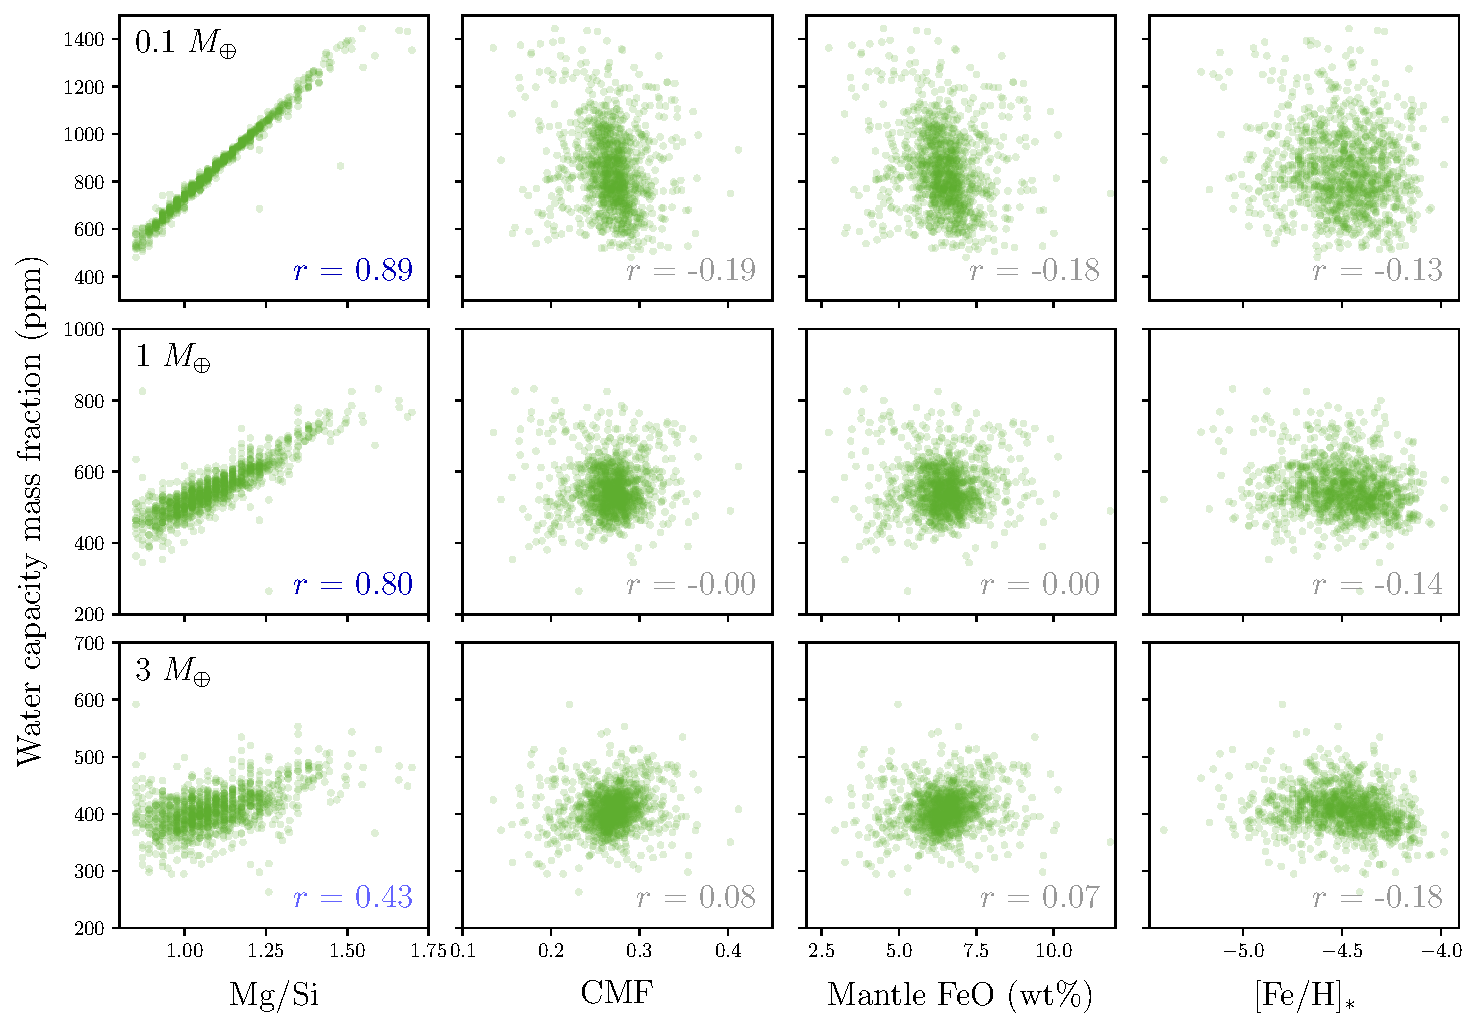
\includegraphics[width=\textwidth]{masses_spread.pdf}
%        \caption{Cross-plots of water capacity (as a fraction of the planet mass), at 0.1 $M_\oplus$ \textit{(top row)}, 0.1 $M_\oplus$ \textit{(middle row)}, and 3 $M_\oplus$ \textit{(bottom row)}, in terms of, from left to right, the molar Mg/Si ratio of the bulk planet, the core mass fraction (CMF), the mantle FeO content in wt.\%, and the host star's logarithmic number ratio of Fe to H. The bulk compositions sampled in this figure are based on all planet-hosting stars in the Hypatia Catalog, excepting low Mg/Si compositions for clarity. All planets are simulated with a constant mantle/core molar Fe partitioning of 0.113 and a potential temperature of 1600 K. The value of the Pearson's correlation coefficient $r$ is given in the bottom right corner of each panel. Water capacities correlate significantly only with Mg/Si; there is a high positive correlation for the 0.1 and 1 $M_\oplus$ cases, and a low positive correlation for the 3 $M_\oplus$ cases.}
%        \label{fig:wmf_scatter}
%\end{figure}
%
%
%\begin{figure}[!h]
%\centering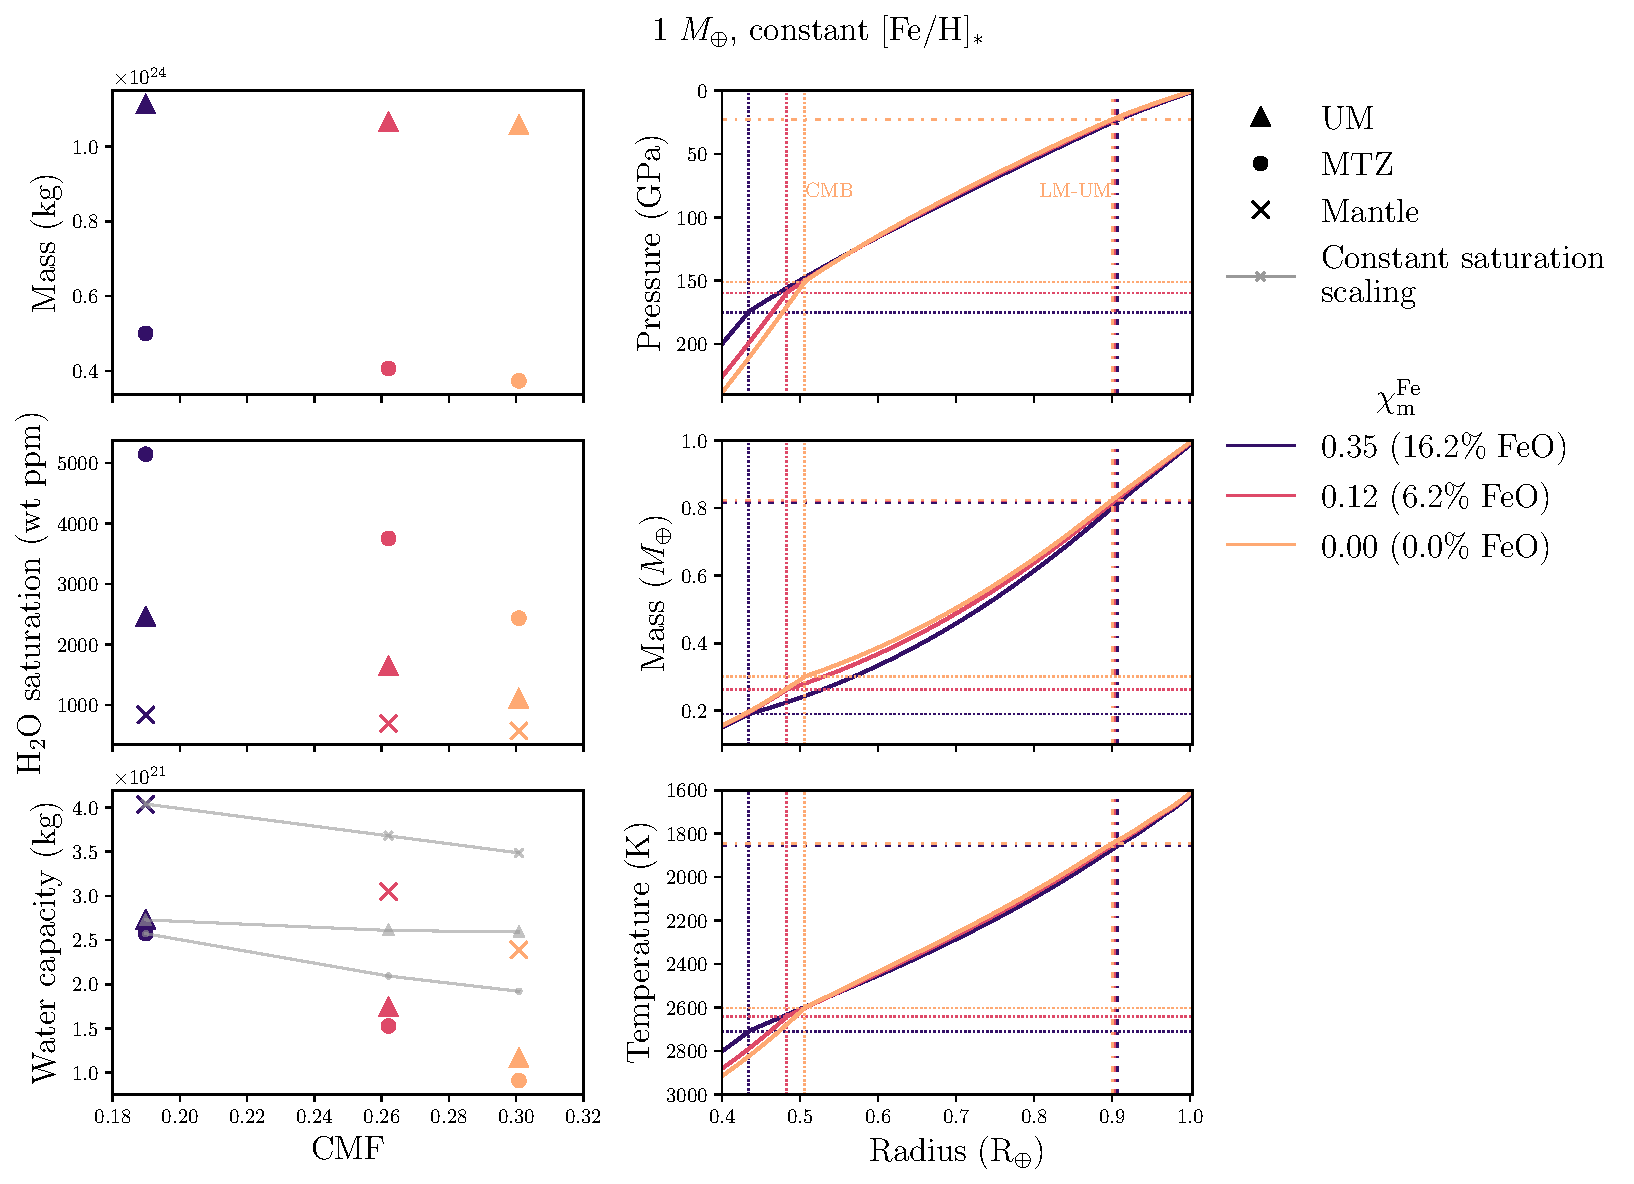
\includegraphics[width=\textwidth]{1M_structure_vs_CMF_coreeff.pdf}
%%%%call your figure name in the place "figurename.eps"
%\caption{The effect on mantle water capacity due to pressure gradients due to planet chemistry. Here we fix the host star and planet's bulk abundance of Fe, [Fe/H]$_*$, but vary molar fraction of Fe in the mantle, $\chi^{\rm Fe}_{\rm m}$. The left column shows, from top to bottom, the layer masses, total water concentrations at water saturation with respect to the layer mass, and water capacities, as a function of the resulting core mass fraction (CMF), for the upper mantle (UM; triangles), mantle transition zone (MTZ; circles), and whole mantle (crosses). In the bottom left panel, the grey lines show the water capacities in kg if mineral water saturations were constant (arbitrarily at the value associated with the lowest CMF), and the only factors affecting water capacities were the masses of the layers. The right column shows, from top to bottom, the profiles of pressure, mass, and temperature through the mantle, with vertical and horizontal lines locating the core-mantle boundary (CMB; dotted lines) and the top of the lower mantle (LM-UM; dash-dotted lines). All cases are fixed to a planet mass of 1 $M_\oplus$ and a potential temperature of 1600 K. In the case of variable $\chi^{\rm Fe}_{\rm m}$, moving iron from the core to the mantle has a small positive effect on the mass of the upper mantle, and a larger positive effect on the mineral water saturation contents, which both act to increase the water capacity.}
%\label{fig:pressure_gradients_coreeff}
%\end{figure}
%
%
%\begin{figure}
%         \centering
%         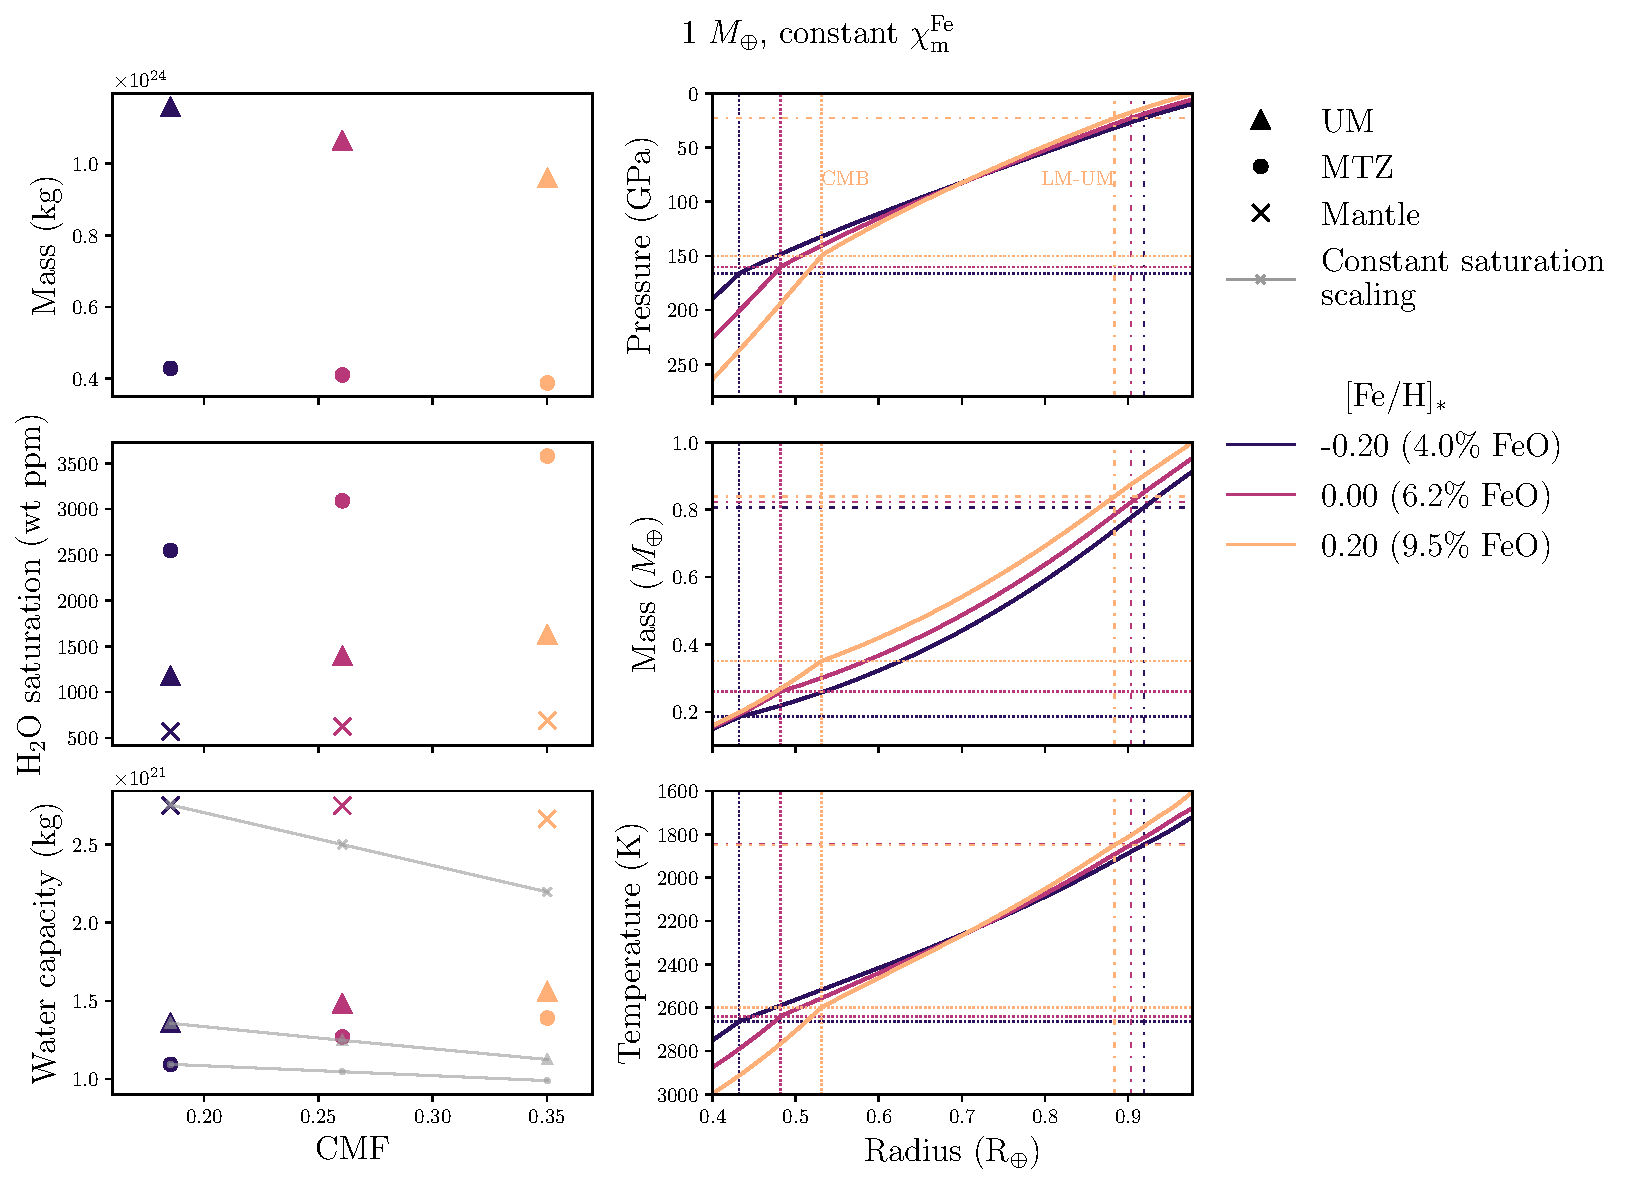
\includegraphics[width=\textwidth]{1M_structure_vs_CMF_feh.pdf}
%         \caption{The same as in Fig. S2, but for a fixed planetary Fe partitioning, $\chi^{\rm Fe}_{\rm m}$, and variable stellar Fe abundance, [Fe/H]$_*$. In the case of variable [Fe/H]$_*$, increasing the overall iron content of the system has a negative effect on the mass of the upper mantle, and a positive effect on the mineral water saturation contents, the results of which nearly cancel out.}
%        \label{fig:pressure_gradients_feh}
%\end{figure}


%!TEX root = ../thesis.tex
%*******************************************************************************
%****************************** Third Chapter **********************************
%*******************************************************************************
\chapter[Modulation of mantle oxygen fugacity by host star refractory abundances]{Modulation of mantle oxygen fugacity by host star refractory abundances, and why exoplanets are not all as oxidising as Earth}
%\chapter{The petrologic modulation of mantle oxygen fugacity, and stellar abundance constraints on why rocky exoplanets are not all as oxidising as Earth}
%\chapter{A petrologic reason for why rocky exoplanets are not all as oxidising as Earth}
\label{chapter:fo2}

% **************************** Define Graphics Path **************************
\ifpdf
    \graphicspath{{Chapter4/Figs/Raster/}{Chapter4/Figs/PDF/}{Chapter4/Figs/}}
\else
    \graphicspath{{Chapter4/Figs/Vector/}{Chapter4/Figs/}}
\fi

\nomenclature[a-fe]{Fe$^{3+}/\Sigma$Fe}{molar fraction of ferric iron to total iron in mantle oxides}
\nomenclature[a-feo]{FeO$^*$}{the sum of \ce{FeO} and \ce{Fe2O3}}
\nomenclature[a-g]{$\Delta G^\circ$}{Gibbs free energy of reaction [${\rm J}\,{\rm mol}^{-1}$]}
\nomenclature[a-k]{$K$}{equilibrium constant (for given reaction)}
\nomenclature[g-m]{$\mu$}{chemical potential [${\rm J}\,{\rm mol}^{-1}$]}
\nomenclature[a-a]{$a$}{thermodynamic activity (of given component)}


\section*{Preface}

At the time of submission, this chapter is currently under review at \textit{Monthly Notices of the Royal Astronomical Society}. After a short author contributions statement, I anticipate that the acccepted manuscript text will not change greatly from that presented here.


\subsubsection*{Contributions and context}

Oliver Shorttle really wanted me to perform these calculations, which follow directly from some of his previous postdoctoral work (published as \citealt{stolper_effects_2020}). The text of this chapter reflects many of Oli's editorial suggestions. My peer Sean Jordan, at the Institute of Astronomy, performed the FastChem modelling that features in the discussion; Fig. \ref{fig:speciation} reflects the contribution from Sean. Finally, John Rudge was as always an important sounding board, and a crucial test reader. Oliver Shorttle, Sean Jordan, and John Rudge will be named as coauthors on the manuscript.



\section*{Abstract}

From core to atmosphere, the oxidation states of elements in a planet shape its evolution. Oxygen fugacity ($f_{\rm O_2}$) is one parameter indicating the likely oxidation state of these elements. With considerable diversity of redox conditions in the solar system planets, we might also expect $f_{\rm O_2}$ to vary among mantles of compositionally-diverse exoplanets. The $f_{\rm O_2}$ of a rocky planet's mantle is set during formation by the relative proportions of iron's different valence states (the dominant multivalent element in planets), yet predicting this distribution \textit{a priori} is a challenge. Here we focus on another factor influencing how oxidising a mantle is---a factor affecting $f_{\rm O_2}$ even when the mantle’s ratio of Fe$^{3+}$ to Fe$^{2+}$ is held constant---the planet’s mineralogy. Changing mineral proportions concentrate the oxidised form of iron, Fe$^{3+}$, within host phases (pyroxenes), increasing its chemical potential and therefore the mantle's $f_{\rm O_2}$. Such mineralogical changes occur within planets according to pressure, and between planets according to their composition. Importantly, inter-planet mineralogical variability is quantifiable because it links to known host star composition. By modelling mineralogical variation, we predict the \textit{minimum} amount by which $f_{\rm O_2}$ could vary between rocky planets from their variable mineralogy alone. We find that the observed stellar Mg/Si distribution has order-of-magnitude effects on mantle $f_{\rm O_2}$, principally through changing proportions of orthopyroxene. This variability is enough to alter by a hundredfold the mixing ratio of SO$_2$ directly outgassed from these mantles. We further predict that planets orbiting high-Mg/Si stars are more likely to outgas detectable amounts of SO$_2$ and H$_2$O; and for low-Mg/Si stars, detectable CH$_4$, all else equal. Even absent predictions of Fe$^{3+}$ budgets, general insights can be obtained into how oxidising an exoplanet’s mantle is. Therefore, even absent an \textit{a priori} prediction of mantle Fe$^{3+}$ abundances, general insights into how oxidising an exoplanet’s mantle and volcanic gases are can be obtained.

\section{Introduction}

Chemical redox equilibria are ubiquitous in all geologic systems. Through the transport of electrons, redox equilibria govern large-scale aspects of the rocky planets built on these systems: from the formation of iron cores \citep{Wood2006, elkins-tanton_coreless_2008, rubie_accretion_2015, lichtenberg_redox_2021}; to the production of magma \citep[e.g.,][]{holloway_highpressure_1992, foley_reappraisal_2011, stagno_oxidation_2013, lin_oxygen_2021}; the supply of volcanic gas, including greenhouse gases \citep[e.g.,][]{kasting_mantle_1993, Delano2001, gaillard_theoretical_2014, ortenzi_mantle_2020, guimond_low_2021,liggins_growth_2022}; and the availability of chemical species for synthesising biologic precursors and catalysing metabolic reactions \citep[e.g.,][]{muchowska_synthesis_2019, wade_temporal_2021}. Thus the surface environments and atmospheres of rocky planets are profoundly influenced by how oxidising their interiors are. This concept, cemented early on \citep{kasting_mantle_1993, HOLLAND2002, kasting_evolution_2003}, is now crucial to bear in mind as we prepare to detect atmospheres on temperate rocky planets, and will hope to distinguish their possible biological origins from geological ones \citep{wordsworth_redox_2018, wogan_abundant_2020, krissansen-totton_oxygen_2021, krissansen-totton_understanding_2022}. The aim of this work is to test whether rocky exoplanets, which are expected to have diverse mantle compositions \citep{hinkel_star_2018, putirka_composition_2019, spaargaren_plausible_2022, guimond_mantle_2023}, will also have more or less oxidising mantles as a consequence. 


\subsection{Quantifying how oxidising a planet's mantle is}\label{sec:quantifying-how-oxidising}

The fugacity of a non-ideal gas like oxygen, \ce{O2}, is the effective partial pressure it would have as an ideal gas with the same chemical potential. This seemingly abstract concept is a powerful tool for quantifying how reducing or oxidising a system is. \ce{O2} appears in numerous redox equilibria in the interiors and at the surfaces of planets: both directly, e.g., in the homogeneous gas phase equilibrium \ce{H2 + 1/2O2 = H2O}; and indirectly as metal oxides' variable valence state, e.g,. in the heterogeneous disproportionation equilibrium \ce{3FeO = Fe + Fe2O3} between three valence states of iron \citep{frost_redox_2008}.  It is through the presence of such equilibria that the fugacity of oxygen (\fo) is constrained and can be quantified. This is possible \emph{even when the system has no free \ce{O2} phase}---\fo\,still remains a measure of how oxidising the system is, by representing the fictive partial pressure of an oxygen gas in equilibrium with the system. 

The processes that influence \fo\,inside a planet are intrinsically linked to the oxidation of Fe, since---as a fact of stellar nucleosynthesis---Fe is by far the most abundant multivalent element found in rocky planets. Therefore, the distribution of Fe between its reduced and oxidised states is interconnected with \fo. We can illustrate this with an inside-out example for planets. 

Hot and partially molten from the energy of accretion, a forming planet's magma ocean might contain Fe co-existing in both its most reduced, metallic, form (Fe$^0$) and its ferrous oxide form (\ce{Fe^{2+}}). The oxidation of iron metal to iron(II) oxide can be written as:
\begin{equation}\label{eq:iw}
\ce{ $\underset{\text{Metallic iron}}{\ce{Fe^0}}$ + \frac{1}{2} O2 <=> $\underset{\text{W\"ustite}}{\ce{Fe^{2+}O}}$ }.
\end{equation}
In our example, the activities, $a$, of Fe-metal and FeO (as dissolved species in the metal and magma phases respectively) would be inter-related with \fo\,through the equilibrium constant of (\ref{eq:iw}):
\begin{equation}\label{eq:K_iw}
K_{(1)} = \exp{\left(\frac{-\Delta G^\circ}{R_bT}\right)} = \frac{a_{\ce{FeO}}}{a_{\ce{Fe}}\left(f_{\ce{O2}}\right)^{1/2}},
\end{equation}
where $\Delta G^\circ$ is the Gibbs free energy of reaction (\ref{eq:iw}) in ${\rm J}\,{\rm mol}^{-1}$, $R_b$ is the gas constant in ${\rm J}\,{\rm mol}^{-1}\,{\rm K}^{-1}$, and $T$ is temperature in K. From the form of (\ref{eq:K_iw}), it can be seen that for a system with magma and metal in equilibrium, this system will have higher \fo---be more oxidising---when there is proportionally more FeO in the magma (assuming for simplicity that the activity of FeO scales with its concentration).
%Firstly, equation (\ref{eq:K_iw}) shows that \todo{$p$ and $T$ have a large influence on absolute \fo. Although simple mole fraction ratios $x_{\ce{Fe}}/x_{\ce{FeO}}$ have previously been used to approximate relative \fo changes with respect to some reference $T$ and $p$, it is hard to imagine that the same relative behaviour holds over many GPa and volume changes are negligible} \citep{righter_redox_2012}. Secondly,

For pure phases of Fe-metal and FeO in equilibrium, the activities in (\ref{eq:K_iw}) would always be unity, offering just one possible \fo\,for a given temperature and pressure. Hence, known \fo\,values of pure compounds in reactions such as (\ref{eq:iw})---the iron-w\"ustite (IW) buffer---are often used as reference values, wherein the \fo\,of a real system is reported as a difference from what this reference \fo\,would be at the temperature and pressure of interest.  %(note this relative \fo\,is only preserved across small $T$, $P$ ranges). 

In a natural system, estimating \fo\,requires knowing the activity of Fe-bearing components in each phase. Magma oceans are highly unlikely to be pure Fe metal and FeO in nature, and calculating these activities and thus absolute \fo, especially at high temperature and pressure, is non-trivial \citep[e.g.,][]{righter_redox_2012}. We can see how this complication comes into the calculation of \fo\,by rewriting the activities in terms of the concentration of the species in the phase, $X_i$, and the rational activity coefficient, $\gamma_i$, which captures departure from ideality. For FeO in a magma from equilibrium \eqref{eq:iw}, ${a^\text{magma}_\text{FeO} = \gamma^\text{magma}_\text{FeO}X_\text{FeO}}$. In this case, whilst $X_\text{FeO}$ would be fixed by the overall amount of oxygen available, the rational activity coefficient may vary as a function of pressure, temperature, and the wider composition of the silicate melt.  As a consequence, \fo\, in this scenario can change \emph{even when the amount of oxygen is constant}; i.e., when ${X_\textrm{Fe}/X_\textrm{FeO}=\textrm{constant}}$.  

The above example makes the point that a complex natural system can become more or less oxidising independently of the amount of oxygen in it. This is true for solid systems of mineral equilibria, as much as for the liquid-liquid `core-forming' equilibria looked at in reaction \eqref{eq:iw}. It is these effects of activity on \fo\,that we investigate in this study, since they can be predicted independently of knowing the (hard to constrain) oxygen budget of the planet---which, simplistically, we consider here to be the ratio of \ce{Fe^{3+}} to \ce{Fe^{2+}} in a mantle rock.
% \todo{Further, reactions between other species in the system may modulate the oxidation state of iron, such that for more complex systems fo2 stops being a clear function of the relative budgets of Fe in its different oxidation states. Namely, the presence of some phases can stabilise Fe3+ where it otherwise wouldn't be. in the deep mantle... iron disproportionation...}

% \todo{therefore, although (1) is sometimes used to describe the CMF of a planet, and this might generally be roughly true given in that this example situation there is minimal effect from other stuff, we need to be careful associating abundance ratios with fO2 because of both volumetric property changes and the stabilising effects of mineral-mineral equilibria}

% here talk about phasehb  stability and dilution. don't nedd to discuss mantle self-oxidation.
\subsection{Mantle mineralogy and \fo}

The objective of this study is to calculate the effect of solid phase equilibria on mantle \fo\,for exoplanets of diverse composition. We are particularly concerned with the \fo\,at the top of an exoplanetary mantle: not only are the thermodynamic data better constrained at these lower temperatures and pressures \citep[$\lesssim 25\,$GPa;][]{guimond_mantle_2023}, but communication with the surface environment is more direct here. Magmas will likely be generated preferentially in the shallow mantle (as on Earth), and consequently, inherit its \fo, which will set the speciation of gases supplied to the atmosphere during volcanism \citep{gaillard_redox_2015, ortenzi_mantle_2020, Liggins2020, guimond_low_2021}. 

Whereas equilibrium \eqref{eq:iw} sets a mantle's \fo\,during core formation, various subsequent mechanisms will likely move the mantle \fo\,away from this initial value \citep[e.g.,][]{frost_experimental_2004, wade_core_2005, Wood2006, williams_isotopic_2012, rubie_accretion_2015, hirschmann_magma_2022}. Through these processes, mantles can become oxidised such that iron exists between its 2+ (FeO) and its more oxidised 3+ (\ce{Fe2O3}) valence states, as is the case for Earth's mantle. The relevant equilibria setting how oxidising a mantle is, near its surface and some time after core formation, therefore involve minerals incorporating iron in these two oxidation states.

A useful reaction for illustrating this scenario is an equilibrium between the minerals olivine, spinel, and quartz. Here, iron can be present as FeO in olivine, as the component fayalite, and as a \ce{Fe2O3} component in spinel, called magnetite:
\begin{equation}\label{eq:qfm}
    \ce{$\underset{\text{Fayalite}}{\ce{3 Fe_2^{2+}SiO4}}$ + O2 <=> $\underset{\text{Magnetite}}{\ce{2 Fe^{2+}Fe2^{3+}O4}}$ + $\underset{\text{Quartz}}{\ce{3 SiO2}}$}.
\end{equation}
If olivine and spinel are solid-solution phases in equilibrium \eqref{eq:qfm}, \fo\,would be modulated upwards if either \textit{(i)} the fayalite component in olivine is diluted by olivine's other constituents (e.g., the forsterite component, \ce{Mg2SiO4}); or \textit{(ii)} the magnetite component is concentrated in spinel, independently of the amount of FeO or \ce{Fe2O3}. This is because concentration or dilution changes the activities of these components.

Like with the example of iron-w\"ustite reaction above, for the pure end-member phases, equilibrium \eqref{eq:qfm} provides a commonly-used reference \fo, that of the fayalite-magnetite-quartz (FMQ) buffer. FMQ has an \fo\,close to that seen in Earth's upper mantle, which is a coincidence resulting from Earth's mantle's composition because Earth's mantle will not have quartz present.
%This is despite orthopyroxene's chemical formula not normally being written with \ce{Fe^{3+}} as a component. Yet together with Al, \ce{Fe^{3+}} can substitute into orthopyroxene as \ce{MgFe^{3+}AlSiO6} \citep{annersten_ferric_1978}, such that an \ce{Fe^{3+}}-bearing component is dissolved in the solid solution that is orthopyroxene. %The extent of \ce{Fe^{3+}} substitution in orthopyroxene itself is independent of \fo\, \todo{(true?? REF)}.

%This fact in itself leads to a crucial part of upper mantle \fo\,variability across different planets. Consider an increase in the proportion of orthopyroxene to Earth's upper mantle's first-most abundant upper mantle mineral, olivine---whose crystal structure takes in no \ce{Fe^{3+}}---whilst keeping the total ratio \ce{Fe^{3+}} to \ce{Fe^{2+}} constant. The larger orthopyroxene mass for the same \ce{Fe^{3+}} mass means that \ce{Fe^{3+}} is diluted in the orthopyroxene solid solution. Hence the activity of the \ce{Fe^{3+}}-bearing component in orthopyroxene decreases---\ce{Fe^{3+}} is less ``reactive". Analogously to $a_{\ce{FeO}}$ in (\ref{eq:K_iw}), \fo\,also must decrease, all else equal.

Quartz is also not expected to be a common mineral in the shallow mantle mineralogies of many rocky exoplanets \citep{spaargaren_plausible_2022, guimond_mantle_2023}. Rather, in most planets as on Earth, it is equilibria among olivine, pyroxenes, garnet, and spinel that set the \fo\,\citep[see][for a detailed review of these effects]{stolper_effects_2020}. The fact that these multi-mineral equilibria govern \fo\,means that the effect of shifting phase proportions on \ce{Fe2O3} activities will everywhere modulate the \fo\,of planetary mantles \citep[e.g.,][]{frost_introduction_1991, oneill_ferric_1993, ballhaus_upper_1995, rohrbach_metal_2007, frost_redox_2008, jennings_simple_2015, stolper_effects_2020}. For Earth, this effect has been investigated in the context of an isochemical mantle (i.e., constant abundance ratio between all oxides, including \ce{FeO} and \ce{Fe2O3}) existing at different pressures, where order-of-magnitude changes in \fo\,were predicted just because of pressure-dependent mantle mineralogy \citep{stolper_effects_2020}. 

Beyond the solar system, however, mineral phase proportions \textit{at a given pressure} will vary significantly according to the bulk mantle oxide proportions of a planet. This mineralogical effect on \fo\,can therefore be calculated for unknown exoplanets by modelling their plausible mineral phase equilibria, based on estimates of their bulk mantle metal oxide compositions, which, are expected to reflect the refractory element ratios observed in their host stars \citep{anders_solarsystem_1982, thiabaud_elemental_2015, bonsor_hoststar_2021}. In this way the chemical ``star-planet connection" \citep{hinkel_star_2018} continues to be explored \citep[e.g.,][]{unterborn_thorium_2015, dorn_can_2015, dorn_generalized_2017, dorn_bayesian_2017, santos_constraining_2017, dorn_new_2019, unterborn_effects_2017, unterborn_pressure_2019, putirka_composition_2019, wang_enhanced_2019, wang_detailed_2022, otegi_impact_2020, spaargaren_influence_2020, spaargaren_plausible_2022, unterborn_mantle_2022, unterborn_nominal_2023, guimond_mantle_2023}. 


%\todo{planet-hosting stellar chemistry variability is a great way to explore what different planetary mantles can look like in general}




 
%Specifically, we expect increasing Mg/Si stoichiometry to increase the olivine/orthopyroxene ratio, and therefore generally increase \fo\,for a constant \ce{Fe^{3+}} budget. Computing the \fo\,distribution that results from the expected variation in bulk composition across exoplanets is the specific aim of this study.


% \todo{ now recall that for a system of solutions, overall fO2 (like in (1)) interrelated to the relative activities of the components of the solutions involved in redox reactions, with the more oxidised form of Fe always on the opposite side of the equilibrium as \ce{O2}. If I increase the pressure and shift these equilibria somewhat, say the relative proportion of opx increases at the expense of ol, whose crystal structure permits no Fe3+, then the activity of the Fe3+-bearing component in opx necessarily decreases. for a constant K fO2 must also decrease. }


\subsection{This study's constraint on exoplanet mantle \fo}

We cannot claim to know \textit{a priori} the ratios of \ce{Fe^3+} to \ce{Fe^2+} in exoplanet mantles, which would be necessary to predict their absolute \fo. A more tractable endeavor is to fix the \ce{Fe^3+}/\ce{Fe^2+} ratio at a nominal value for all planets, and calculate the \textit{variability} of \fo\,due directly to phase equilibria; i.e., the changes in how \ce{Fe^3+} is distributed between co-existing mineral phases and the impact of this on \fo. We go on to show that this variability is largely independent of the chosen \ce{Fe^3+}/\ce{Fe^2+} ratio. By this method we hence produce an estimate of the minimum variability in mantle \fo\,across exoplanets: \fo\,must differ by \textit{at least} this much because of mineralogy alone.

Because this \fo\,constraint is obtained from modelling mantle phase equilibria directly, our approach is complementary to previous work by \citet{ortenzi_mantle_2020} and \citet{liggins_growth_2022}, who explored the possibility of inferring mantle \fo\,from anticipated spectroscopic observations of exoplanet atmospheres---certain patterns of gas species in a volcanic atmosphere would in principle link to how oxidising the mantle source is. As for direct observational prospects, \citet{doyle_oxygen_2019, doyle_where_2020, doyle_new_2023} report measurements of FeO abundances in planetary material at the end of its life, accreted in fragments onto white dwarfs. Such measurements could link to the bulk Fe oxidation state of the original parent body given some knowledge about how its iron inventory was partitioned between metal and oxides. Accurately retrieving the oxygen abundances in polluted white dwarfs remains difficult, however, due to time-variability during accretion \citep{brouwers_asynchronous_2023}.

We present a first \textit{a priori} constraint on the variability of mantle \fo\,across exoplanets, stemming directly from refractory abundance distribution in the Hypatia Catalog of nearby stars \citep{hinkel_stellar_2014}. In section \ref{sec:methods-mineralogy}, we outline our method of calculating upper mantle mineralogy and the associated \fo\,from bulk mantle compositions, and in section \ref{sec:methods-bulkcomp}, of converting from stellar refractory element abundances to these bulk mantle compositions. Section \ref{sec:results} presents the resulting distributions and various compositional correlations of \fo. Section \ref{sec:discussion} discusses a consequence for planetary evolution; namely, the speciation of outgassed volatiles. Section \ref{sec:fo2-conclusion} concludes the study.


\section{Methods}



\subsection{Phase equilibria and oxygen fugacity}\label{sec:methods-mineralogy}

We use two independent models to calculate phase equilibria at pressures $P \in [1\,,4]\,{\rm GPa}$, and temperature $T = 1373\,{\rm K}$, for a wide sample of hypothetical exoplanet bulk mantle compositions. Although we expect these two models to result in different values of absolute $f_{\ce{O2}}$---due to differences in how they incorporate \ce{Fe^3+} into minerals and treat mineral solid solutions---we will show that the compositional variation in $f_{\ce{O2}}$ is robust to choice of database. There are three components to each model: \textit{(i)} the codes that solve for the stable mineralogy and mineral compositions; \textit{(ii)} the thermodynamic databases, which contain data on endmember mineral component entropies, etc.; and \textit{(iii)} activity-composition relations, or ``mineral models'', that describe the solid solutions and their thermodynamics. 

First, we use the pMELTS software package and its native thermodynamic database and mineral model \citep{asimow_algorithmic_1998, ghiorso_pmelts_2002}. For numerical stability, all calculations are initialised at superliquidus conditions, $2273\,{\rm K}$. Then the system is cooled along the desired isobar in 5-K increments, until the $T$ of interest is reached. The target temperature was chosen to be well below the solidus of typical rocky planet mantles. However, some mantles are predicted to still contain a small fraction of liquid, which will be having a small effect on the estimated \fo.  We therefore exclude any mantle compositions with a remaining liquid phase in excess of 1 wt.\% at the $T$ of interest. About 50 compositions fail to converge at subsolidus temperatures with pMELTS and no stable phase assemblage can be found. 

We perform a second set of calculations using the \citet{jennings_simple_2015} thermodynamic database and mineral model implemented in the code Perple\_X \citep{connolly_geodynamic_2009}; hereafter, JH-15. These calculations are done in the constrained minimisation mode of Perple\_X, at the $T$ and $P$ of interest.

% we need to be clear that there are three things here: the codes that solve for the stable mineralogy and mineral compositions
% 1) the codes that solve for the stable mineralogy and mineral compositions.  The 'solvers'
% 2) the thermodynamic databases, which contain data on endmember mineral component entropies etc.
% 3) activity-composition relations, or 'mineral models' that describe the solid solutions and the thermodynamics of these.  
% JH-15 is a particular choice of database + solution models.  pMELTS is database + models + solver all together.

Perple\_X and pMELTS calculate the relative proportions of stable phases by minimising the Gibbs free energy for an input wt.\% bulk oxide composition (section \ref{sec:methods-bulkcomp}), over an input $T$ and $P$. We consider cases where the solution phases olivine, orthopyroxene, clinopyroxene, spinel, and garnet comprise $\sim$100\% of the mineralogy between 1--$4\,{\rm GPa}$. We exclude any bulk compositions that stabilise a pure-\ce{SiO2} phase (e.g., quartz, coesite) due to less-well-constrained thermodynamic data (see section \ref{sec:discussion-sio2}). We further exclude the handful of compositions where pMELTS stabilises extraneous phases, such as kyanite or rhombohedral-oxide solution. Our choice of pressure endpoints excludes crustal phases whilst spanning the important spinel-garnet transition in the upper mantle. 

We note that the hypothetical planet's mass is not directly relevant for our calculations, given we are fixing $T$, $P$; the only implicit constraint on planet mass therefore is that it be large enough to have mantles reaching $4\,{\rm GPa}$ (for context, Mars, 1/10 the mass of Earth, has a mantle pressure up to $19\,$GPa at its base; \citealt{stahler_seismic_2021}).  The direct effect of planet mass in this framework is therefore just to change the depth in km corresponding to the pressure of interest. In practice, planet mass may have influenced the oxygen budget of the mantle \citep[e.g.,][]{frost_redox_2008}, but such effects are not considered in this study.

\subsubsection{Absolute oxygen fugacity from chemical potentials}

The fugacity of \ce{O2} is related to its chemical potential, $\mu$, at the $T$ and $P$ of interest, relative to the standard state chemical potential, $\mu_0$, at 1 bar and the $T$ of interest:
\begin{equation}\label{eq:mu_fo2}
\log f_{\ce{O2}}= \frac{\mu - \mu_0} { R T \ln(10) } + \log a,
\end{equation}
where $R = 8.3145\,{\rm J\, mol}^{-1}\,{\rm K}^{-1}$ is the gas constant, $T$ is temperature in K, and $a$ is the thermodynamic activity of \ce{O2}. We set $a = 1$ \citep{stolper_effects_2020}, so the last term on the right hand side disappears. Thus by adopting a fixed $T$ and $P$, we can perform meaningful comparisons of \fo\,between different bulk compositions.  

The pMELTS software internally calculates $\log f_{\ce{O2}}$ at each $T$ and $P$ of interest \citep[see][]{asimow_algorithmic_1998}. Meanwhile, Perple\_X only returns $\mu$, so here we explicitly use (\ref{eq:mu_fo2})\,to find $\log f_{\ce{O2}}$, with $\mu_0$ calculated via the same JH-15 database.


\subsubsection{Relative oxygen fugacity using buffers}

Because oxygen fugacities strongly depend on $T$ and (less so) $P$, it is convenient to report them as a difference in dex with respect to the value of $\log f_{\ce{O2}}$ produced by a known buffer reaction---such as (\ref{eq:iw}) or (\ref{eq:qfm})---at the same $T$ and $P$ of interest. For relatively modest changes in $T$ and $P$, intrinsic $\log f_{\ce{O2}}$ differences between system and buffer will be approximately preserved, thus largely normalising out the direct effect of temperature on $\log f_{\ce{O2}}$. 
%Because buffers tend to follow roughly parallel $\log f_{\ce{O2}}$ paths through $P$-$T$ space (within a range). Therefore the $T$ and $P$ information can often be elided.\footnote{See \citet{righter_redox_2012} for discussion of when this approximation breaks down.}
Hence we will also report most of our calculations as a relative $\log f_{\ce{O2}}$ with respect to FMQ (\ref{eq:qfm}), denoted $\Delta$FMQ. 

We calculate $\log f_{\ce{O2}}$ of FMQ using JH-15, and subtract the absolute $\log f_{\ce{O2}}$ from pMELTS or JH-15 to find $\Delta$FMQ. We emphasise, however, that the $\Delta$FMQ values we find are not necessarily meaningful, only their distribution.

\subsection{Mantle bulk composition from stellar element abundances}\label{sec:methods-bulkcomp}

Our method of converting stellar abundances to phase proportions is essentially the same as in \citet{guimond_mantle_2023} and discussed there in more detail. 

We take the entire sample of planet-hosting FGKM stars from the Hypatia Catalog \citep{hinkel_stellar_2014} which have measured Mg, Si, Fe, Ca, Al, Na, and Ti, using the reported mean if a star has been measured more than once. Here, the normalised stellar abundance of an element X with respect to hydrogen is reported as:
\begin{equation}\label{eq:nH_star}
    {\rm [X/H]} = \log(n_{\rm X}/n_{\rm H})_{\star} - \log(n_{\rm X}/n_{\rm H})_{\sun},
\end{equation}
where $n$ is the number abundance, the subscript $\star$ denotes the value for the star, and the subscript $\sun$ denotes the solar value from \citet{lodders_abundances_2009}. We conserve the relative number abundances of Mg, Si, Fe, Ca, Al, Na, and Ti between the star and the bulk planet.

Within planet interiors, these seven elements together with oxygen will occur as component oxides (e.g., MgO, \ce{SiO2}) of mantle mineral phases, which constitute virtually its entire mass. We place most of the bulk Fe as a metallic planetary core, leaving an unconstrained but minority fraction as Fe oxide in the mantle. That is, we assume that there is enough O available to bond with all of the Mg, Si, Ca, Al, Na, and Ti; we do not track the affinity of O for rocky or volatile/icy material in the protoplanetary disc. Because the extent of Fe oxidation is unknown \textit{a priori}, we use a free parameter $f^{\rm Fe}_{\rm mantle}$~=~\xcore\;which defines the molar ratio of FeO$^*$ in mantle oxides to the total bulk planet Fe---here and throughout we use FeO$^*$ to mean the sum of iron oxides regardless of the valence state of iron (2+ or 3+), whilst FeO denotes ferrous iron oxide alone. We initially use a fixed value of $f^{\rm Fe}_{\rm mantle} = 0.12$ (that reproduces Earth's core mass fraction for pure, solid Fe), but later test the effects of varying $f^{\rm Fe}_{\rm mantle}$ on the distribution of \fo.

% higher p-t core formation can increase mantle FeO content through Si reduction (Siebert et al. 2012; Fischer et al. 2015),

To find the bulk composition of the mantle in weight percent, being the required input to the thermodynamic models, we convert the abundance of each element [X/H] to its wt.\% equivalent, conserving the total moles of Fe as described in \citet[n.b. here we interpret their FeO as FeO*]{guimond_mantle_2023}.

Planetary mantles will only inherit their host star [X/H] if element X is perfectly refractory. Ca, Al, Mg, Si, Fe, and Ti are highly refractory, so we apply our stellar abundance-to-mantle oxide method at face value (but removing some Fe to the core as above). For Na, which is more volatile, as a first guess we approximate a depletion factor: we calculate the molar ratio of Na/Ti in the bulk silicate Earth \citep{workman_major_2005} relative to Na/Ti in the solar photosphere \citep{lodders_abundances_2009}, and scale [Na/H] by this constant planet/star depletion factor of 0.046 across all systems. \citet{spaargaren_plausible_2022}, in a similar attempt to relate stellar to planetary compositions, additionally account for possible Si in the core and for the slightly higher volatility of Mg versus Si, and hence produce slightly different Mg/Si ratios than our model. The effects of secondary processing on mantle Mg/Si ratios do not affect our \fo\,variability results, but are briefly discussed in \ref{sec:discussion-mgsi}.% Whilst we do not include this effect, the compositional trends we present allow the effect of differential Mg/Si volatility to be interpreted in terms of \fo\,change.

The bulk mantle compositions resulting from this method will be approximations of the true composition of a planet; caveats are discussed more extensively in \citet{guimond_mantle_2023}. However, because it allows us to cover a large sample (\textgreater 1000) of observed stellar compositions, our approach can provide a useful estimate of the corresponding breadth of mineralogically-driven \fo\,variation, regardless of the true median which is in any case beyond our reach. %\todo{also, because we are interested in the range and can't pin down \fo\,anyways, small changes in mineralogy due to partitioning processes we don't capture will not matter for our resulting distributions, they might just shift the whole thing}





\subsubsection{Nominal ferric iron content}

To calculate \fo\,emerging from Fe redox equilibria, we must specify, as thermodynamic components in the system, either FeO$^*$ and \ce{O2} (Perple\_X input), or \ce{FeO} and \ce{Fe2O3} (pMELTS input). Both ways of describing the composition of the system are equivalent, as some amount of nominal \ce{O2} in fact forms ferric iron to create a unique molar ratio of FeO to \ce{Fe2O3} (again,  assuming no other multivalent, redox-active elements are present in the system). From the stoichiometry of the simple redox reaction \ce{4FeO + O2 <=> 2Fe2O3}, we have 2 mol \ce{Fe2O3} for every mol \ce{O2}, and 2 mol \ce{Fe^3+} for every mol \ce{Fe2O3}, so the effective molar abundance of \ce{O2} is: 
\begin{equation}\label{eq:x_ferric}
n_{\ce{O2}} =  \frac{1}{4}\left(\ce{Fe^{3+}}/\Sigma \ce{Fe}\right) n_{\ce{FeO}^*},
\end{equation}
where \xfer\;is the molar ratio of ferric iron to total iron in the (bulk) mantle, and $n_{\ce{FeO}^*}$ is the molar abundance of Fe in mantle oxides as required by stellar element abundances and $f^{\rm Fe}_{\rm mantle}$. 

Equivalently, we can find the component mass fractions of \ce{FeO} and \ce{Fe2O3} by simultaneously solving:
\begin{equation}\label{eq:m_fe2o3}
\begin{split}
\ce{Fe^{3+}}/\Sigma \ce{Fe} &= \frac{2m_{\ce{Fe2O3}} / M_{\ce{Fe2O3}}}{m_{\ce{FeO}} / M_{\ce{FeO}} + 2m_{\ce{Fe2O3}} / M_{\ce{Fe2O3}}}\\
m_{\ce{FeO}^*} &= m_{\ce{FeO}} + m_{\ce{Fe2O3}},
\end{split}
\end{equation}
where $m$ denotes the mass in kg and $M$ the molar mass in ${\rm kg}\,{\rm mol}^{-1}$ for the subscripted species.

In this way, a fixed \xfer\;is imposed across all compositions: for Perple\_X runs \ce{O2} is added to make up the required \xfer\;given FeO$^*$ using (\ref{eq:x_ferric}); or, for pMELTS runs, FeO$^*$ is divided into FeO and \ce{Fe2O3} using (\ref{eq:m_fe2o3}). Note that in either case the total mass or number amount drops out once the bulk composition is re-normalised to 100\%. Earth's mantle \xfer\;value of 3\% would be equivalent to having 8.2 wt.\% \ce{FeO} react with 0.027 wt.\% \ce{O2}. 

Note that different choices of \xfer\;will have a minor effect on equilibrium mineralogy. Increasing \xfer\;from 3\% to 10\%, for example, increases the amount of orthopyroxene by a few wt.\% at the expense of clinopyroxene. %, in effect decreasing the ratio of olivine to orthopyroxene from 1.86 to 1.50 \todo{at XX $T,P$}. 
However, the amount of mineralogically-derived variability in mantle \fo\,is roughly preserved across different values of \xfer, as we will show.


\begin{figure}
\centering
  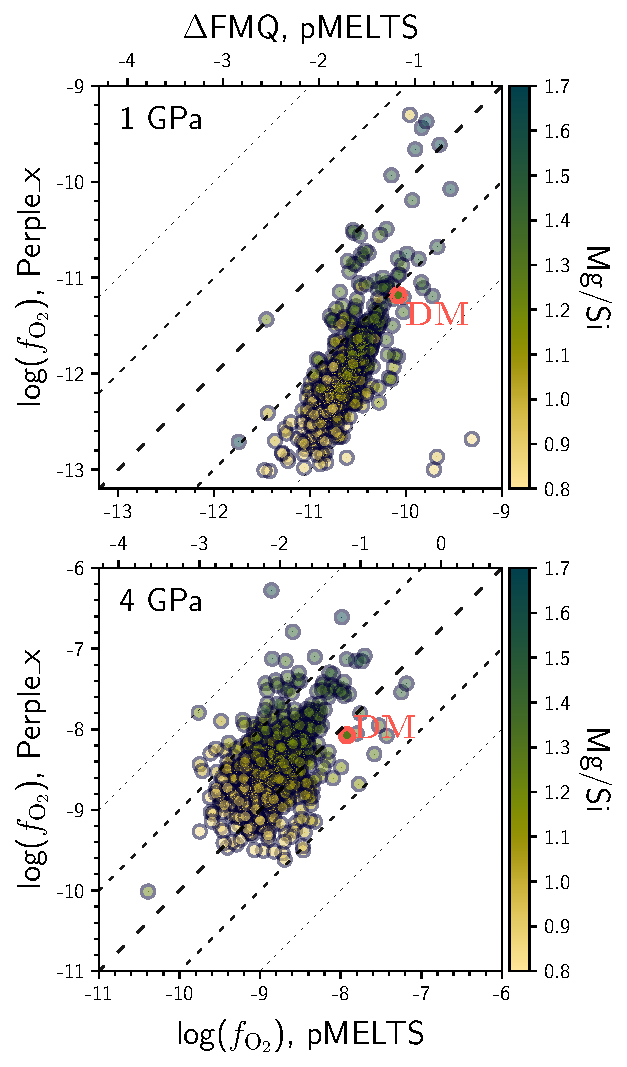
\includegraphics[width=0.7\linewidth]{logfo2_mdls_pressures.pdf}
\caption[Direct comparison of absolute \fo\,between the pMELTS and Perple\_X models.]{\label{fig:model_comp}Direct comparison of absolute \fo\,between the pMELTS and JH-15 in Perple\_X models, at $1\,\text{GPa}$ \textit{(top)} and $4\,\text{GPa}$ \textit{(bottom)} and $1373.15\,\text{K}$. Each point represents the bulk mantle composition inferred from a planet-hosting star in the Hypatia Catalog, assuming ${\rm Fe}^{3+}/\Sigma{\rm Fe} = 3$\% and $f^{\rm Fe}_{\rm mantle} = 12$\%. Earth's depleted mantle (DM) composition from \citet{workman_major_2005} is highlighted in red for comparison. Points are coloured by the molar Mg/Si ratio. Both models' compositions are in terms of MgO, \ce{SiO2}, \ce{Al2O3}, \ce{CaO}, \ce{Na2O}, \ce{Cr2O3}, \ce{FeO}, and \ce{Fe2O3}; pMELTS has \ce{TiO2} in addition.}
\end{figure}


\subsubsection{Choice of oxide components}\label{sec:methods-components}

The major rock-forming oxides MgO, \ce{SiO2}, CaO, \ce{Al2O3}, and FeO$^*$ should make up \textgreater~99\% of exoplanetary mantles by mass---considering only these components would suffice if our only goal were to estimate phase abundances. However, other minor oxides can potentially have a non-negligible influence on mantle \fo, either by stabilising important ferric iron-hosting phases at different $T,P$, or affecting \ferric\,substitution in crystal structures. Hence, as in \citet{stolper_effects_2020}, we also consider \ce{Na2O} and \ce{TiO2}, and in one set of reference calculations, \ce{Cr2O3}. 

Although the presence of \ce{Na2O} has minor effects on orthopyroxene phase proportions in both pMELTS and JH-15 (changing them by $\lesssim10$ wt.\%), this can lead to disproportionately large effects on \fo. Including \ce{TiO2} in the pMELTS runs is necessary to ensure that numerically-stable subsolidus phase assemblages can be found for most bulk compositions. Meanwhile, JH-15 can only place \ce{TiO2} in a pure rutile phase, so for Perple\_X runs we exclude \ce{TiO2} from bulk compositions in the thermodynamic modelling, although we still retrieve stellar Ti to calculate the Na depletion as discussed above. Minor amounts of \ce{Cr2O3} affect \ferric\,substitution into pyroxenes, whilst stabilising spinel at slightly higher pressures, allowing Earth's upper mantle \fo\,to be reproduced more accurately from Earth's depleted mantle composition.



% \todo{we assume  \textit{(i)} the major upper mantle species are expected to be broadly similar in presence \citep[e.g.,][]{putirka_composition_2019, spaargaren_plausible_2022, guimond_mantle_2023}, and \textit{(ii)} among these phases, pyroxenes and spinel or garnet will always be the only hosts of \ce{Fe^{3+}}.}









\section{Results}
\label{sec:results}


\begin{figure*}
\centering
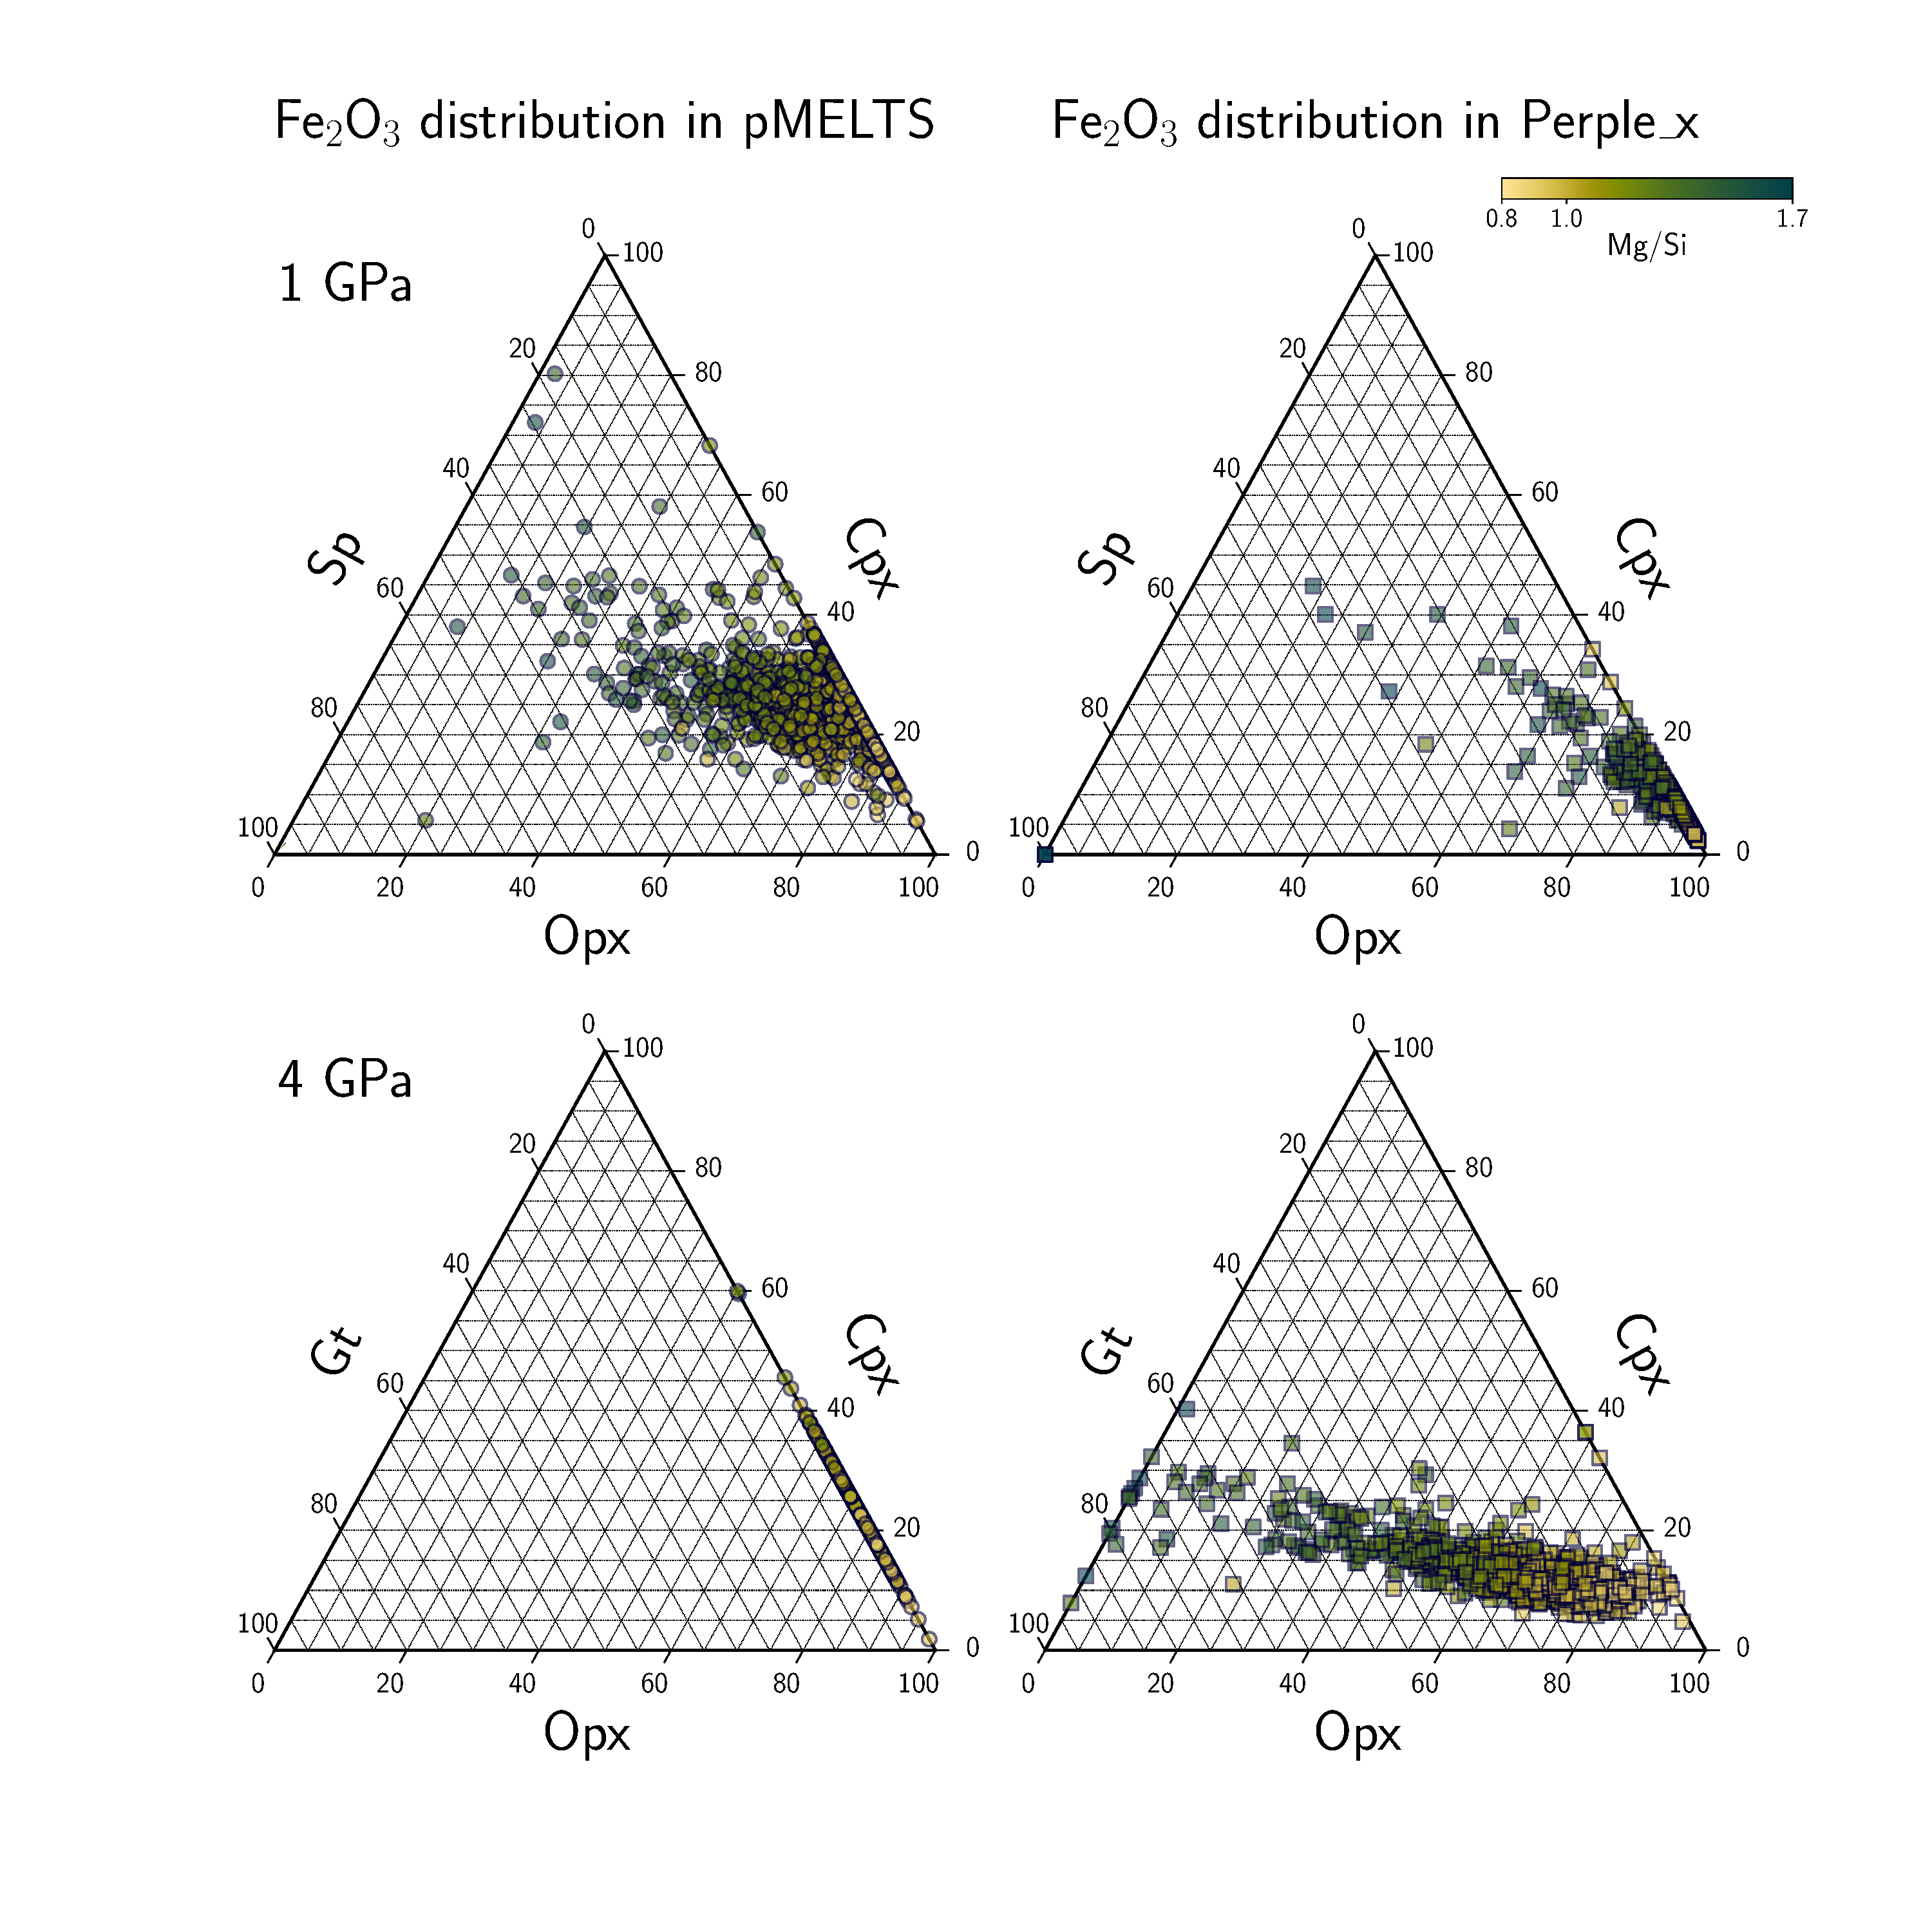
\includegraphics[width=1\textwidth]{ternary_subplots.pdf}
\caption[Ternary diagram showing the distribution of \ce{Fe2O3} between its subsolidus host phases.]{\label{fig:ferric_ternary}Ternary diagram showing the distribution (modality) of \ce{Fe2O3} between its subsolidus host phases: orthopyroxene (Opx), clinopyroxene (Cpx), and spinel (Sp) or garnet (Gt), at $1\,{\rm GPa}$ \textit{(top)} and $4\,{\rm GPa}$ \textit{(bottom)} and $1373.15\,\text{K}$. Olivine contains no \ce{Fe^3+} in either of the thermodynamic databases we consider. Fe$_2$O$_3$ modality is calculated as the weight fraction of \ce{Fe2O3} in each phase, multiplied by the phase's total weight fraction in the system, and normalised to 100\% between the three phases on each axis. The right column shows results from pMELTS, and the left column shows Perple\_X results. Each point represents a bulk mantle composition (Ca-Na-Fe-Mg-Al-Si-O, plus Ti in pMELTS) inferred for a planet-hosting star in the Hypatia Catalog. Points are coloured by Mg/Si. Note that the horizontal guides correspond to the Cpx axis.}
\end{figure*}


\begin{figure*}
\centering
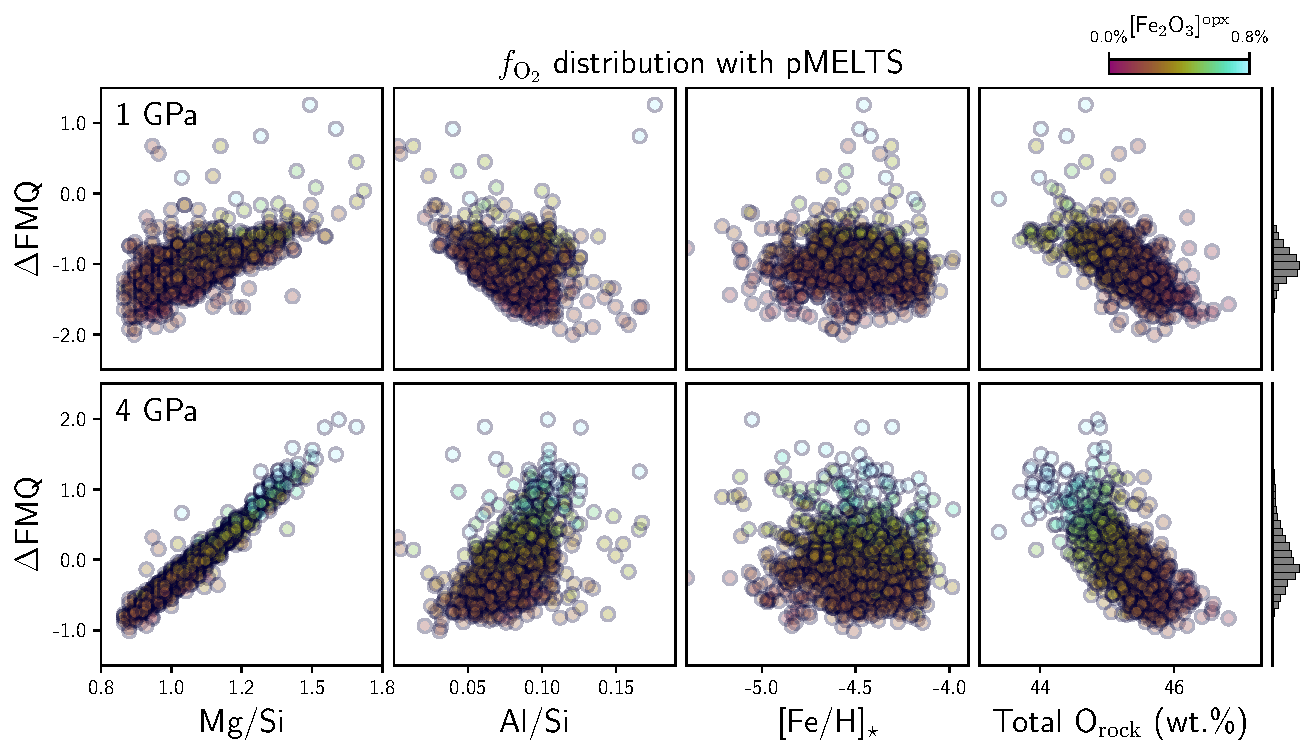
\includegraphics[width=1\textwidth]{crossplot_xtra_melts.pdf}
\caption[Cross plots of log($f_{\ce{O2}}$) with various compositional parameters from pMELTS.]{\label{fig:xplots_mlts}Cross plots of log($f_{\ce{O2}}$) expressed as $\Delta$FMQ, resulting from pMELTS calculations, shown at $1\,{\rm GPa}$ \textit{(top)} and $4\,{\rm GPa}$ \textit{(bottom)} and $1373.15\,\text{K}$. From left to right, columns show the dependence of \fo\,on bulk mantle Mg/Si, Al/Si, stellar metallicity [Fe/H]$_\star$, and the total refractory oxygen present in the mantle, O$_{\rm rock}$ (i.e., a sum over oxygen in all metal oxides). Each point ($N = 1198$) represents a bulk mantle composition (Ca-Na-Fe-Mg-Al-Si-O-Ti) inferred for a planet-hosting star in the Hypatia Catalog, assuming ${\rm Fe}^{3+}/\Sigma{\rm Fe} = 3$\% and $f^{\rm Fe}_{\rm mantle} = 12$\%. Points are coloured by the \ce{Fe2O3} wt.\% composition of orthopyroxene (opx). Histograms of the $\Delta$FMQ distribution are projected on the $y$-axis.}
\end{figure*}

\begin{figure*}
\centering
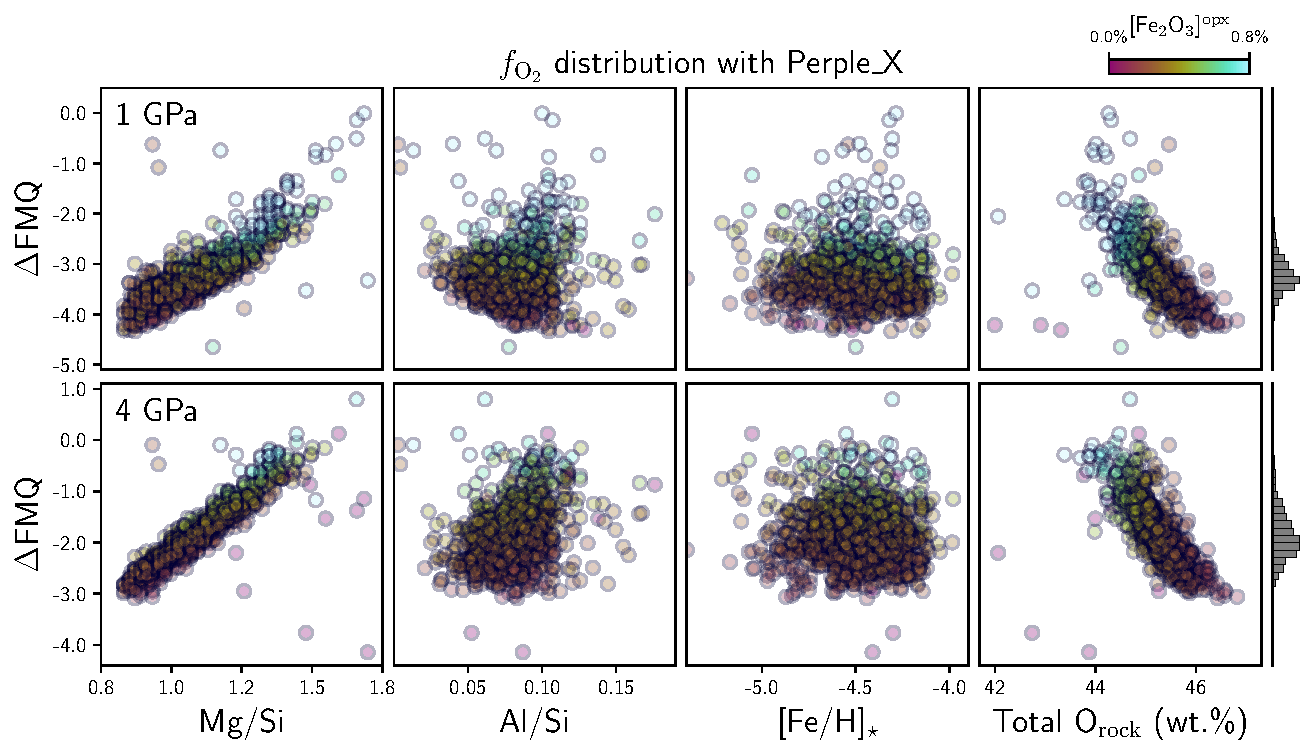
\includegraphics[width=1\textwidth]{crossplot_xtra_perplex.pdf}
\caption[Cross plots of log($f_{\ce{O2}}$) with various compositional parameters from Perple\_X.]{\label{fig:xplots_px}The same results as presented in Figure \ref{fig:xplots_mlts}, but using the JH-15 database in Perple\_X (and excluding Ti from bulk compositions; $N = 1206$). Note the different $y$-axis scales.}
\end{figure*}



\subsection{The host minerals of ferric iron in planetary mantles}\label{sec:results-ferric-hosts}

JH-15 and pMELTS model the thermodynamics of ferric iron incorporation into mineral phases as particular \ferric-bearing mineral endmembers. The models differ in the endmembers they use, their solution models, and the thermodynamics of those solution models. From this fundamental description of the minerals emerges partitioning behaviour of \ferric\;(and other elements). These important differences in how the models we use are constituted leads to systematically different absolute \fo\,between them for a given bulk composition, sometimes by 2 dex (Figure \ref{fig:model_comp}). So not only is predicting \fo\,hard for a planetary mantle without prior knowledge of its ferric iron abundance, it is challenging even when we can assume its ferric iron abundance. However, we will show that between the two models we use, \textit{(i)} the amount of \fo\,variation is similar, and \textit{(ii)} the compositional dependence of the \fo\,variation is also similar. As we are focusing on \fo\,variability arising from changes in bulk mantle composition, the fact that the models agree on this suggests the ensuing insights are robust.

%\todo{Figure \ref{fig:model_comp}, not really sure how much this is adding other than illustrating perplex systematically gives lower fo2 compared to pmelts, seemingly because in pmelts ferric iron can partition into spinel. no spinel at 4 Gpa so difference is smaller here.}

The main phenomenon causing \fo\,to vary for constant bulk mantle \xfer\;is that different minerals can take characteristically different amounts of ferric iron into their crystal structures. We illustrate this phenomenon with a series of ternary diagrams (Figure \ref{fig:ferric_ternary}), showing \ce{Fe2O3} modality for each bulk composition inferred from our Hypatia sample, to better understand the origins of the \fo\,variations produced by pMELTS and JH-15. Ternary diagrams are useful for plotting three variables which sum to unity, as is the case here. 

At $1\,\text{GPa}$, the stable phases that incorporate \ferric\,are orthopyroxene, clinopyroxene, and spinel (note an olivine phase is almost always present yet contains no \ferric). Each point in the top row of Figure \ref{fig:ferric_ternary} shows the mass fraction of \ce{Fe2O3} in those phases for a given mantle composition, weighted by the mass fraction of the phase itself in the system. The fact that most points plot near the bottom-right corner shows that orthopyroxene is the most important \ferric\;host in almost all compositions at $1\,\text{GPa}$, for both models. Although spinel's crystal structure may incorporate higher fractions of \ce{Fe^3+}, when spinel is stable, its overall abundance rests at a few percent, and so has limited scope to affect the local \fo. In fact, the JH-15 model produces some mineralogies with very small spinel abundances, so many points in the top right panel of Figure \ref{fig:ferric_ternary} plot very close to the right edge of the diagram ($\sim$0\% spinel axis).

At $4\,\text{GPa}$---bottom row of Figure \ref{fig:ferric_ternary}---spinel has been replaced by garnet, which has different \ferric\,partitioning behaviour. Further, unlike spinel, garnet can start to form sizeable proportions of the mantle at a few GPa, especially for the more Al-rich planetary compositions. In the JH-15 model, orthopyroxene exchanges \ferric\,with garnet (although not shown, more \ferric\,partitions into garnet with increasing $P$). Meanwhile, the pMELTS model does not place \ferric\,into garnet, hence all points in the bottom left panel of Figure \ref{fig:ferric_ternary} plot on the $\sim$0\% garnet axis. Although assessing which model (pMELTS or JH-15) is more ``realistic''---the differences between them are discussed thoroughly in \citet{stolper_effects_2020}---it is worth mentioning that in this case, \ferric\,is indeed observed in mantle-derived garnets \citep[e.g.,][]{quinn_accurate_2016}.

 %\todo{[which is more realistic, do we know? Oli: There is ferric iron in garnet.  So in this sense the JH15 model is more realistic]} %There is also a secondary effect of Al3+ exchange between gt and px, which substitutes with Fe3+ \citep{stolper_effects_2020}.  

Note that in order to reproduce the Earth's present-day upper mantle (``depleted mantle'') \fo\,near to FMQ, the calculations in Figure \ref{fig:model_comp} included \ce{Cr2O3} in the bulk compositions. The presence of the minor cation \ce{Cr^{3+}} can significantly influence \ce{Fe^{3+}} partitioning (even without affecting modal mineralogy; see section \ref{sec:methods-bulkcomp}). However, all subsequent calculations omit \ce{Cr2O3} because \textit{(i)} Cr is moderately volatile (hence less-related to the stellar abundance), and \textit{(ii)} Cr measurements are less-frequently listed in the Hypatia stellar compositions ($N$ = 636 in the Figure \ref{fig:model_comp} sample). The deceivingly large effect of minor cations on \fo\,highlights the fact that absolute \fo, along with being model-dependent, cannot be constrained precisely without detailed compositional information. For example, the depleted mantle composition in Figure \ref{fig:model_comp} would be 1 log unit more oxidised without Cr in the pMELTS model at $1\,\text{GPa}$.



\subsection{Compositional correlations of \fo}

Given that the majority of \ce{Fe2O3} is in orthopyroxene for most planetary mantle compositions (Figure \ref{fig:model_comp}) and the proportion of \ce{Fe2O3} in olivine is always zero, it follows that the main predictor of upper mantle \fo\,for a given \xfer\,would be the olivine/orthopyroxene ratio. A greater olivine/orthopyroxene ratio concentrates the mantle's \ferric\,budget into orthopyroxene, thus raising the activity $a_{\rm Fe_2O_3}^{\rm opx}$ (compare (\ref{eq:K_iw})). The olivine/orthopyroxene ratio will be itself strongly positively correlated with Mg/Si \citep{hinkel_star_2018, spaargaren_plausible_2022, guimond_mantle_2023}, a fact of these phases' chemical stoichiometries: the Mg-endmember of olivine \ce{Mg2SiO4} (forsterite) requires 2 atoms of Mg per atom Si, while the Mg-endmember of orthopyroxene \ce{MgSiO3} (enstatite) requires 1 atom Mg per atom Si. Thus, excess Mg with respect to Si builds olivine-dominated mineralogies. Magnesium and silicon have this dominant role in setting planetary mineralogy simply because of their high cosmochemical abundance.

Figures \ref{fig:xplots_mlts} and \ref{fig:xplots_px} show the relationship between \fo\,(as $\Delta$FMQ) and Mg/Si, plus various other parameters describing bulk planet composition, for pMELTS and JH-15 respectively. A key result is that despite the differences between the two models (section \ref{sec:methods-mineralogy}), they nonetheless predict fundamentally similar systematics between \fo\,and planetary parameters. We emphasise that \xfer\;and thus the real \fo\,is unconstrained for exoplanets; we fix \xfer\;at 3\% for the sake of creating these figures. The Mg/Si effect that we have explained in the previous paragraph induces $\sim$3 orders of magnitude variation in mantle \fo\,(left-most columns). The scatter in \fo\,versus Mg/Si at $1\,\text{GPa}$ is wider due to slightly more complicated phase equilibria at the lower pressures; pMELTS further places more \ferric\;into spinel, with more scope for affecting \fo\,(Figure \ref{fig:ferric_ternary}). We find that the correlation of $\Delta$FMQ with Mg/Si at $1\,{\rm GPa}$ has a slope of 1.40 and 3.05, in pMELTS and JH-15 respectively, and at $4\,{\rm GPa}$, 3.37 and 3.98 (Supplementary Figure \ref{fig:mgsi_fit}).

The relationship between Al/Si and \fo\,is more complex (Figures \ref{fig:xplots_mlts} and \ref{fig:xplots_px}, second columns), but again consistent between models. In pMELTS and JH-15 the correlation with \fo\,is negative in the spinel field, yet positive in the garnet field. Several effects lead to this behaviour and are discussed more thoroughly in \citet{stolper_effects_2020}. Most directly, Al-rich compositions stabilise mantles with higher proportions of the aluminous phases spinel and garnet, and less pyroxene (Supplementary Figure \ref{fig:alsi_opx}). In pMELTS at high pressure, where garnet does not take any \ferric, the \ce{Fe2O3} activity in orthopyroxene therefore increases with increasing Al/Si. In JH-15, \ferric\,is redistributed between garnet and orthopyroxene, so the trend is less straightforward and the correlation between \fo\,and Al/Si becomes weaker. Similarly at $1\,\text{GPa}$, larger proportions of spinel dilute the \ferric-bearing component in this aluminous phase, which can have a bearing on \fo.


The third columns of Figures \ref{fig:xplots_mlts} and \ref{fig:xplots_px} demonstrate how no correlation exists between upper mantle \fo\,and stellar Fe abundance (metallicity, [Fe/H]$_\ast$), at a fixed molar distribution of planetary iron between \ce{Fe^0}/\ferrous/\ferric. Increasing the total Fe in planetary mantles does not significantly affect the partitioning of ferric iron between minerals in pMELTS and JH-15; the ratios of \ce{Fe2O3} and \ce{FeO} activities in host minerals are independent of total Fe.

Lastly, in the fourth columns, we show the correlation between \fo\,and the total mass percent of refractory oxygen bound as metal oxides (e.g., O in \ce{SiO2}, \ce{CaO} etc.), which we call the total O$_{\rm rock}$ (wt.\%). Both models show that total O$_{\rm rock}$ is strongly negatively correlated with mantle \fo\,at both pressures. This seemingly counter-intuitive negative correlation is a stoichiometric effect aliasing the Mg/Si effect above; it arises from the valence state of the metal oxides forming the planet's mantle. As Mg occurs as MgO and Si as \ce{SiO2}, higher Mg/Si favours forsterite (\ce{Mg2SiO4}), which is 45.5\% O by mass, over enstatite (\ce{MgSiO3}), which is 47.8\% O by mass. Because planets with higher Mg/Si will have higher ratios of forsterite to enstatite, they will therefore have lower total O$_{\rm rock}$ for stoichiometric reasons, whilst having higher \fo\,for thermodynamic reasons. Further discussion of the Mg/Si ratio's effect on the amount of refractory O that condenses to form planets can be found in \citet{unterborn_effects_2017}.



\subsection{Minimum variability of \fo\,across mantle compositions}

% \todo{compare perplex and alpha melts - violin plots of increasing pressure isothermally}


The previous subsections set up an understanding of the \fo\,variability caused by changing mineral proportions in the upper mantles of rocky exoplanets. We call our distributions a minimum variability because observations of exoplanet host star chemistry imply that these mineralogies should indeed vary across exoplanets \citep{hinkel_stellar_2014, putirka_composition_2019}. The true variability of \fo\,will be broader than what we report here if \xfer\;also varies across exoplanet mantles---empirically true, at the very least,  considering Earth and Mars \citep[e.g.,][]{dale_late_2012}. The extent of iron metal core segregation, $f^{\rm Fe}_{\rm mantle}$, could also plausibly affect upper mantle \fo\,through its effect on mineralogy. We have therefore calculated exoplanet mantle \fo\,distributions as a function of these two key unknown parameters, \ce{Fe^{3+}}/$\Sigma$Fe and $f^{\rm Fe}_{\rm mantle}$ (Figures \ref{fig:hist_fe} and \ref{fig:hist_core} respectively). Here, data in each histogram encompass the same stellar abundance data for known exoplanet host stars ($N$ between 976 and 1232 for pMELTS, and between 1033 and 1251 for JH-15), but varying the fixed parameter \xfer\;or $f^{\rm Fe}_{\rm mantle}$. We choose generous prior ranges of these parameters to test naive extremes of their underlying distributions.


\begin{figure*}
\centering
  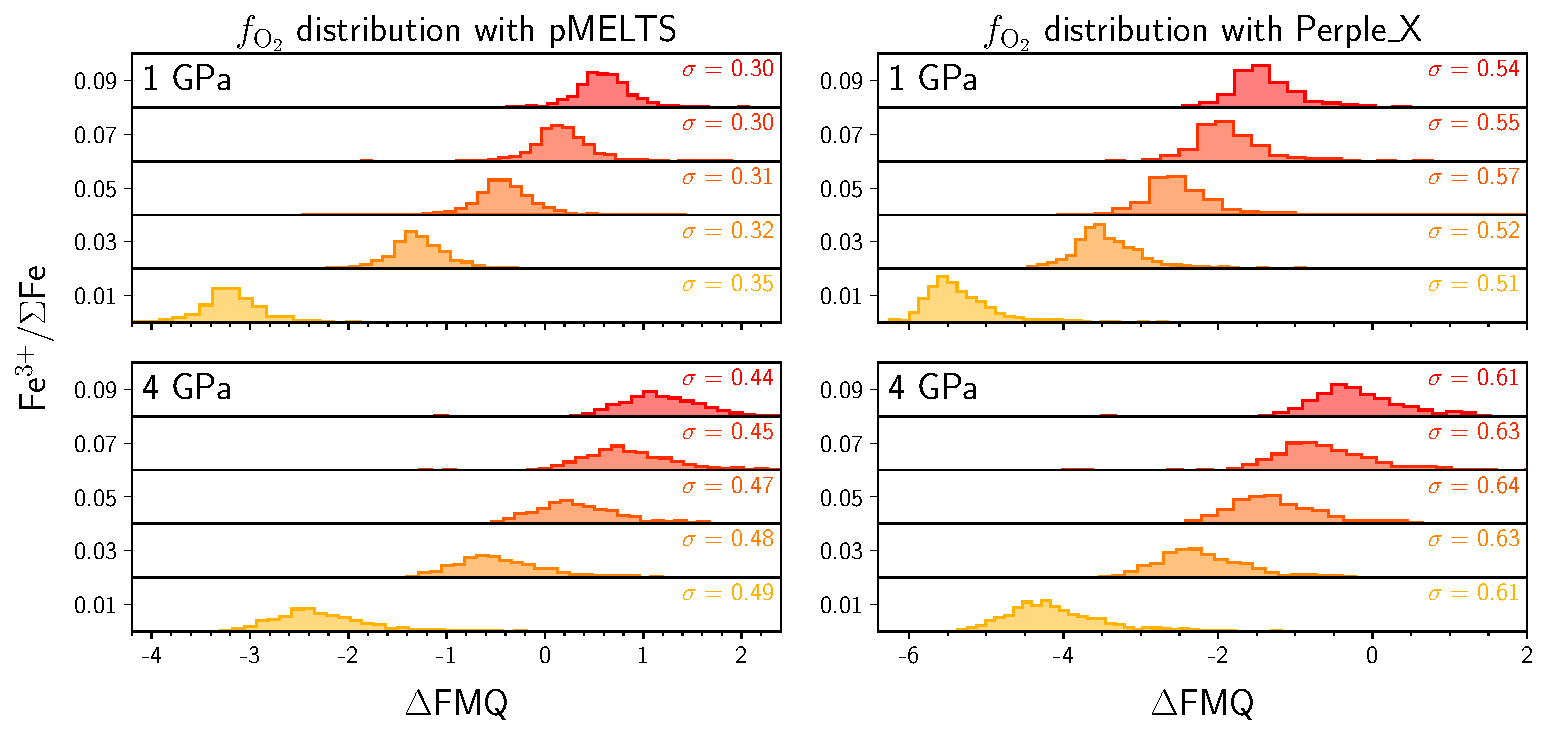
\includegraphics[width=\textwidth]{hist_X_ferric.pdf}
\caption[The distributions of mantle oxygen fugacities resulting from stellar chemical variability: dependence on \ce{Fe^{3+}}/$\Sigma$Fe.]{The distributions of mantle oxygen fugacities expressed as $\Delta$FMQ, resulting from chemical variability in Hypatia host stars. Distributions are shown for different mantle \ce{Fe^{3+}}/$\Sigma$Fe ratios and assuming $f^{\rm Fe}_{\rm mantle} = 12$\%, at $1\,{\rm GPa}$ \textit{(top)} or $4\,{\rm GPa}$ \textit{(bottom)}, using the pMELTS \textit{(left)} or JH-15 in Perple\_X \textit{(right)} models. Calculations are shown at $1473\,{\rm K}$ to ensure more compositions have numerically-stable solutions. Standard deviations $\sigma_{f\text{O}_2}$ of each distribution are shown in the upper right corners.\label{fig:hist_fe}}
\end{figure*}
\begin{figure*}
\centering
  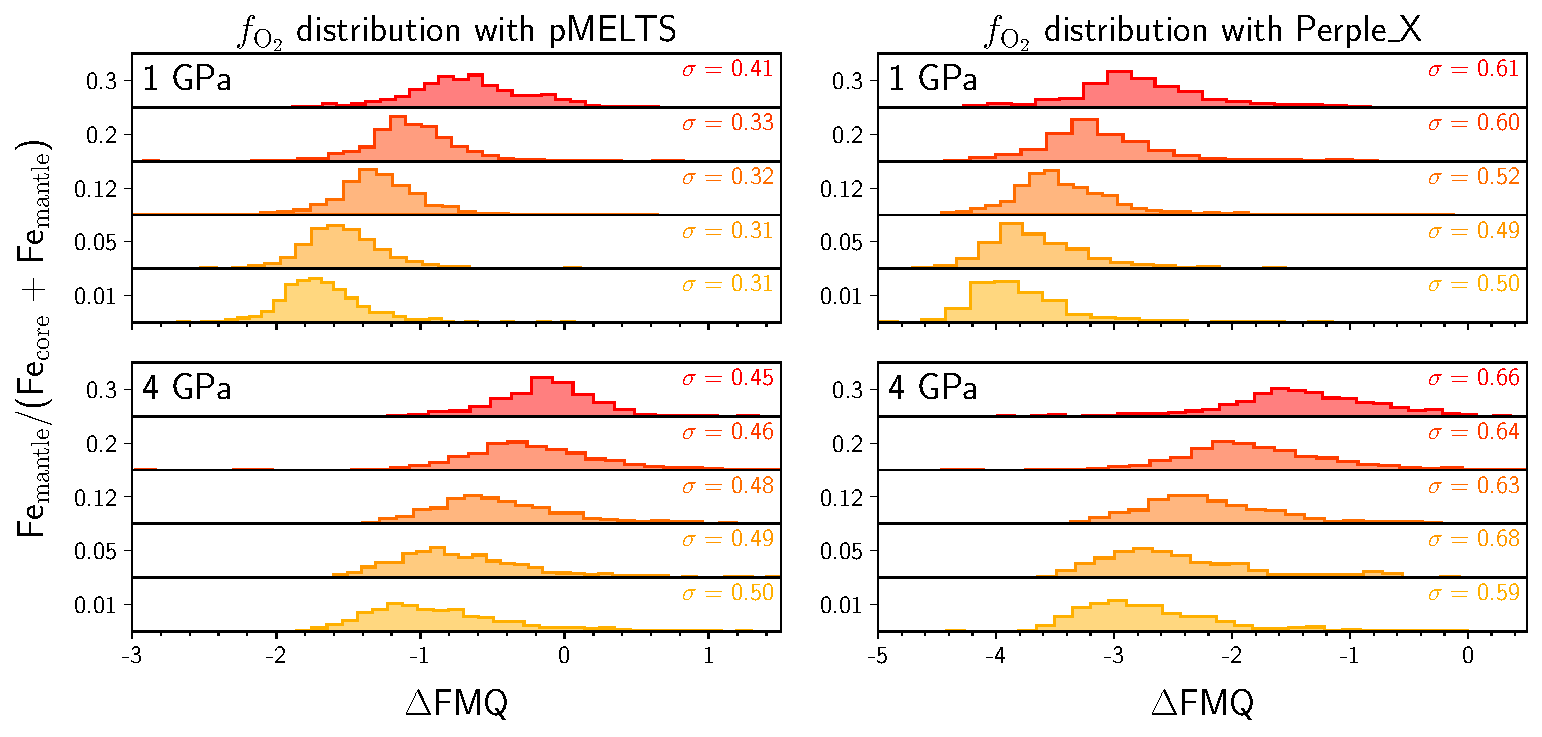
\includegraphics[width=\textwidth]{hist_core_eff.pdf}
\caption[The distributions of mantle oxygen fugacities resulting from stellar chemical variability: dependence on the extent of core formation.]{The same as Figure \ref{fig:hist_fe}, but showing $\Delta$FMQ distributions for different assumptions about the bulk planet iron partitioning ${\rm Fe}_{\rm mantle}/({\rm Fe}_{\rm core} + {\rm Fe}_{\rm mantle}) = f^{\rm Fe}_{\rm mantle}$, for mantle ${\rm Fe}^{3+}/\Sigma{\rm Fe} = 3$\%. Note the different $x$-axis scales between models and between here and Figure \ref{fig:hist_fe}.\label{fig:hist_core}}
\end{figure*}





As expected, increasing \xfer\;means increasing \ce{Fe2O3} activities and therefore \fo. Figure \ref{fig:hist_fe} shows 2\%-increments of \xfer: as it increases from 1\% to 9\%, $\Delta$FMQ increases by about 4 log-units. Yet the widths of the \fo\,distributions, represented by their standard deviations, appear similar, $\sigma_{f\text{O}_2} \approx 0.3$ dex at $1\,\text{GPa}$ and $\sigma_{f\text{O}_2} \approx 0.4$ dex at $4\,\text{GPa}$. The lack of strong dependence of $\sigma_{f\text{O}_2}$ on (a reasonable range in) Fe oxidation state supports our ability to estimate a minimum \fo\,\emph{variability}.% It would be unlikely to find \xfer\,$\gg$ 10\% \todo{because [????????]}. 

All distributions in Figure \ref{fig:hist_fe} are wider at $4\,\text{GPa}$ compared to $1\,\text{GPa}$ due to the stability of garnet, which generally has higher modality than the lower-pressure aluminous phase spinel, and thus has more scope for affecting \ferric\,activities. In detail, distributions are also slightly wider at the lowest \ferric. The non-linearity of median \fo\,versus \xfer\;is due to the fact that $\Delta$FMQ is logarithmic.%We attribute this effect to the log-scale of $\Delta$FMQ. \todo{[confirm with unlog fo2, also check phase stability?] ---an effect also seen in .}



In Figure \ref{fig:hist_core}, each histogram now represents a different choice of $f^{\rm Fe}_{\rm mantle}$. Whilst \xfer\;affects \ferric\,activities directly, $f^{\rm Fe}_{\rm mantle}$ merely changes the wt.\% FeO$^*$ of the mantle. Note that no compositions stabilise a Fe-metal phase in the upper mantle, so only FeO and \ce{Fe2O3} activities are relevant for \fo\,(cf. \eqref{eq:K_iw}: in the much-more-reducing magma ocean, $f^{\rm Fe}_{\rm mantle}$ is actively linked to \fo\,via equilibria between Fe$^0$ and Fe$^{2+}$). 

Increasing total FeO$^*$ will slightly increase the olivine/orthopyroxene ratio, but otherwise has only a passive influence on \fo. Figure \ref{fig:hist_core} shows that greater $f^{\rm Fe}_{\rm mantle}$ is associated with a generally higher \fo\,at constant \xfer, which is explained by this stabilising effect of FeO$^*$ on olivine, therefore concentrating the \ferric\,in orthopyroxene (clinopyroxene, spinel, and garnet proportions are unaffected). Again, $\sigma_{f\text{O}_2}$ is similar across the large range of $f^{\rm Fe}_{\rm mantle}$; these distributions are reliable estimates of minimum \fo\,variabilities. The slight row-wise differences in $\sigma_{f\text{O}_2}$ do not follow the same pattern between pressures and thermodynamic datasets, which points to the complex effects of FeO$^*$ on phase stability and resulting \ferric\,activities.% and hence on \ce{FeO} and \ce{Fe2O3} activities.

%As we increase $\chi_{\rm Fe}^{\rm mantle}$, slight differences in $\sigma_{f\text{O}_2}$ have the opposite sense of change between 1 and 4 GPa and between thermodynamic datasets.%The effect of \xcore\,on median \fo\,could be amplified if we consider that higher Mg/Si in the protoplanetary disk means more refractory O is condensed and mantles are richer in FeO$^*$ for the same stellar O abundance \citep{unterborn_effects_2017}.





\subsubsection{Relevance of the core mass fraction for upper mantle \fo}

A final observation from the experiments in Figures \ref{fig:hist_fe} and \ref{fig:hist_core} is the relative importance of \xfer\;and $\chi_{\rm Fe}^{\rm mantle}$. Doubling \xfer\;from an Earth-like value increases the median $\Delta$FMQ by more than one log-unit; the same $\Delta$FMQ increase would require a much greater change in $\chi_{\rm Fe}^{\rm mantle}$. If we compare Figure \ref{fig:hist_core} with Figures \ref{fig:xplots_mlts} and \ref{fig:xplots_px}, it is clear that the direct effect of stellar abundance variability on exoplanets' upper mantle $\Delta$FMQ is more significant than the direct effect of the planets' unknown extent of core formation within the range we consider.

That is, the core mass fraction of a planet is not necessarily a proxy for its \textit{upper mantle} \fo. The equilibrium between Fe-metal and FeO that governs core size is generally no longer operating in the evolved uppermost mantle, if Fe-metal is not present here to buffer electron transfer. The direct relevance of a larger core mass fraction is just to take away from the total mantle iron budget. There are of course indirect effects (beyond the olivine stability mentioned above) in that the physical processes controlling core size may themselves impact the mantle \xfer\;(that is, $\chi_{\rm Fe}^{\rm mantle}$ and \xfer\;are probably not independent of one another in reality). For example: \textit{(i)} larger cores come at the expense of high-pressure silicate phases in the lower mantle, phases which may be important for producing \ferric\;in planetary interiors; and \textit{(ii)} certain processes that may affect the mantle \ferric\;budget would be more effective at oxidising the mantle when the mantle is more iron-poor, such as \ce{H2O} photolysis followed by \ce{H2} loss. These effects are discussed in section \ref{sec:discussion-ferriciron}.



\section{Discussion}
\label{sec:discussion}


\subsection{The effect of mantle \fo\,variability on volcanic gas chemistry}



\begin{figure*}
\centering
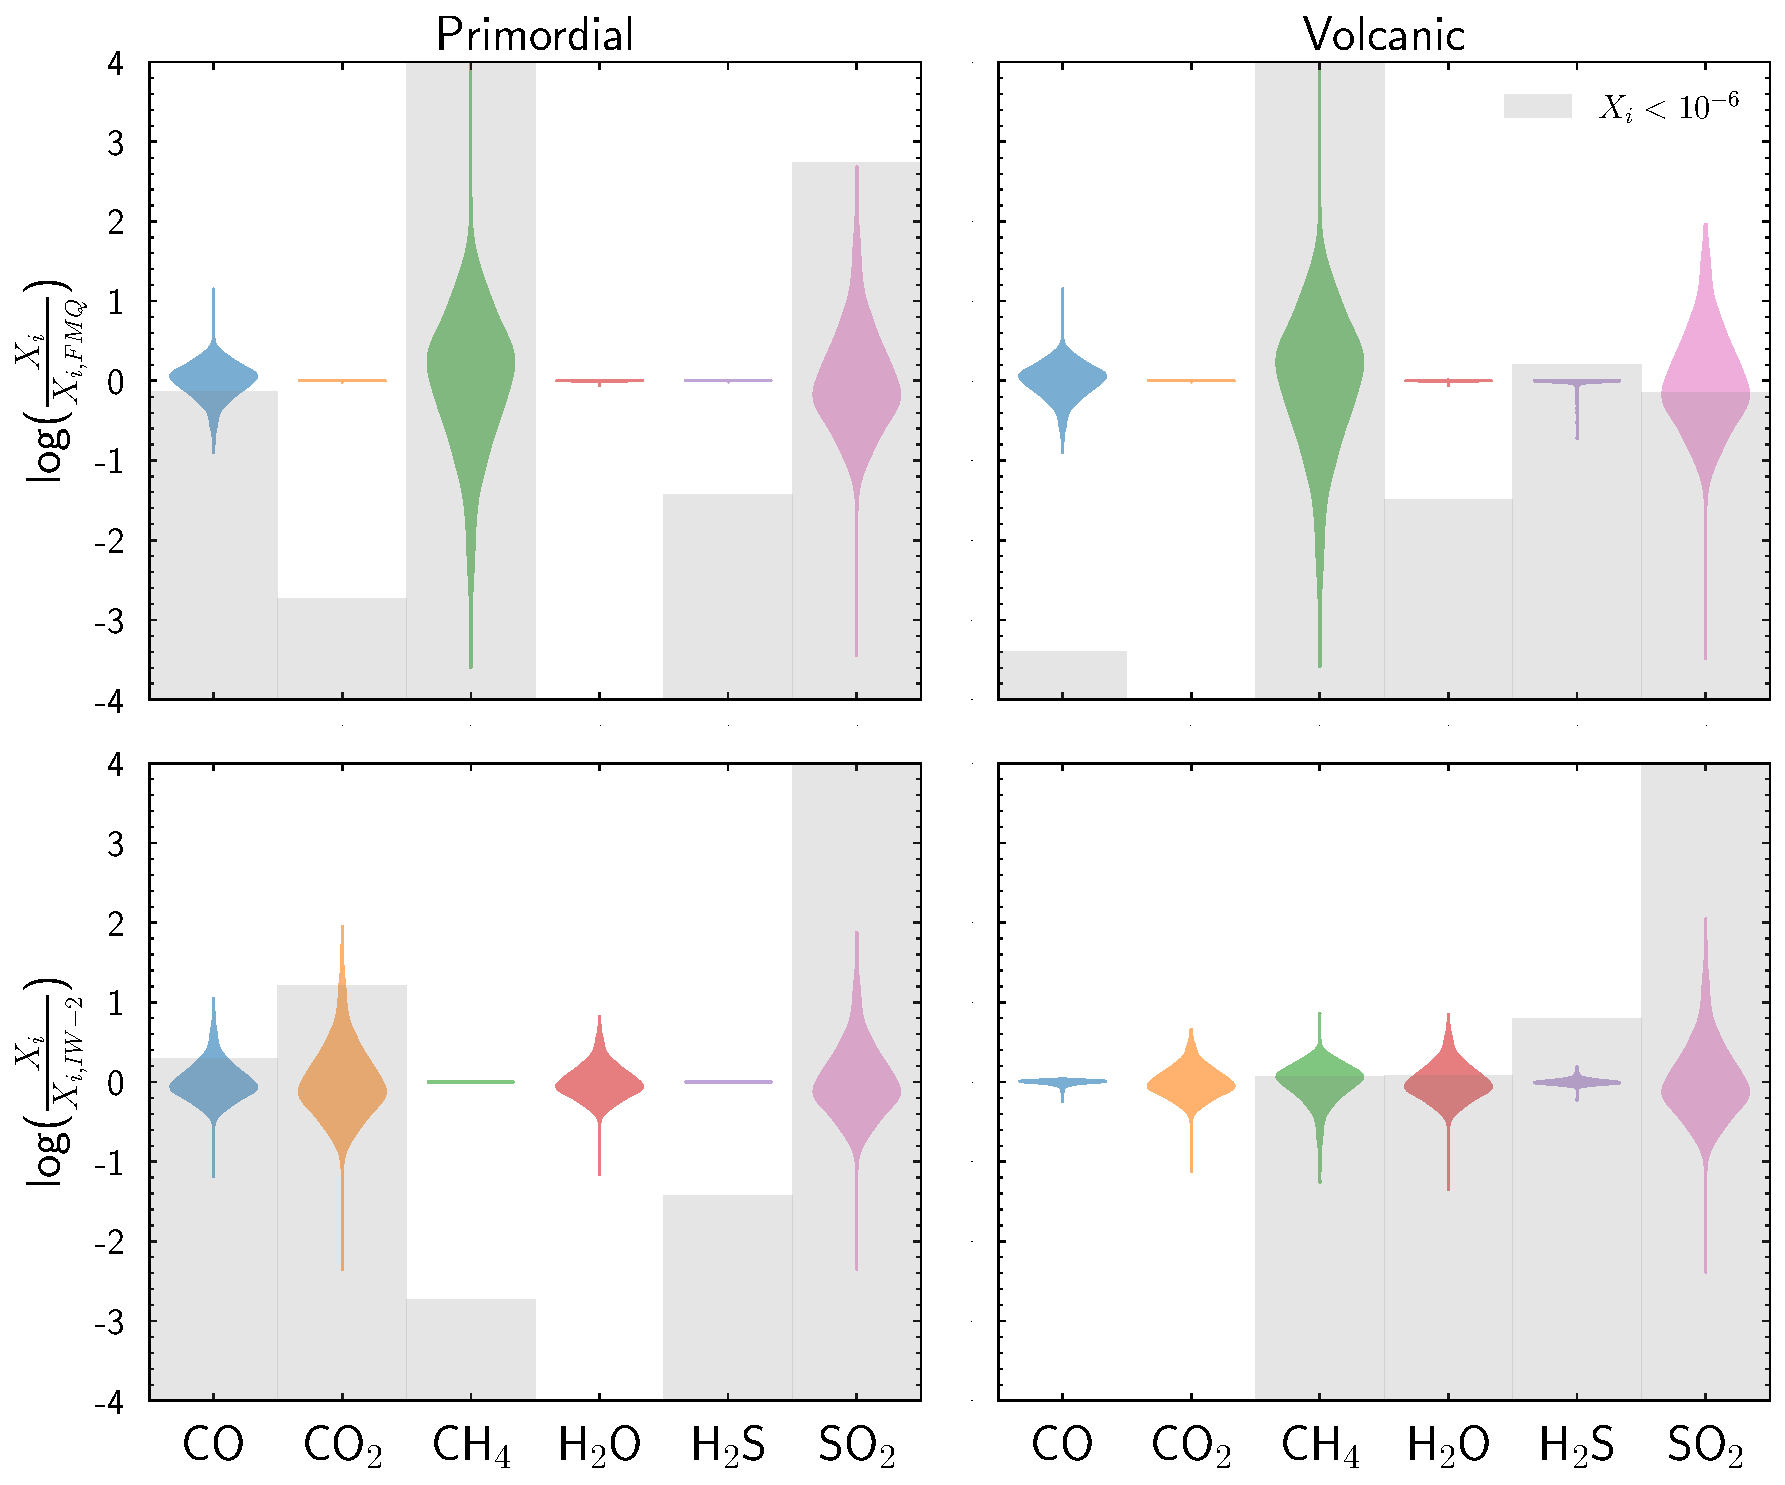
\includegraphics[width=1\textwidth]{violins.pdf}
\caption[The variability of volcanic gas mixing ratios, or molar concentrations, which are a direct result of the calculated variability of exoplanet mantle \fo.]{\label{fig:speciation}Violin plots of the variation in volcanic gas speciation resulting from our calculated mantle \fo\,variability. Speciation is expressed as the the mixing ratio $X$ at the calculated \fo, relative to what the mixing ratio would be at a reference \fo---either FMQ (modern Earth's upper mantle; \textit{top}) or ${\rm IW} - 2$ (Earth's mantle at core formation; \textit{bottom})---with distributions normalised such that the median \fo\,is that of the reference. Distributions are shown for two nominal bulk atmosphere C-S-H ratios: a primordial composition \textit{(left)} reflecting the protoplanetary disk, and a volcanic composition \textit{(right)} reflecting Venus' present-day atmosphere. The grey patches show where mixing ratios are less than 1 ppm and therefore likely below the detection limit in an exoplanet atmosphere. This example calculation uses our \fo\,distribution from pMELTS at 4 GPa (nominally representative of melting below a stagnant lid), projected to a degassing temperature and pressure of 800 K and 1 bar.}
\end{figure*}


Our discussion focusses on one implication of the minimum mantle \fo\,variability that we have estimated, being volcanic gas speciation. Volatile species such as \ce{CO2} and CO, \ce{H2O} and \ce{H2}, and \ce{SO2} and \ce{H2S} are carried to a planet's surface by magmas, maybe building up volcanic atmospheres \citep[e.g.,][]{gaillard_theoretical_2014,liggins_growth_2022}. Gases that exsolve from magmas have their redox chemistry set by the magma's \fo; the magma will have inherited its \fo\,in turn from its (upper) mantle source region. The \fo\,of the source therefore buffers the gas-phase equilibria \citep[e.g.,][]{kasting_mantle_1993, burgisser_redox_2007, gaillard_redox_2015}:
\begin{align}
    \ce{H_2 + 1/2O2 &<=> H_2O},\label{eq:h-gas}\\
   \ce{CO + 1/2O2 &<=> CO_2},\label{eq:c-gas}
\end{align}
where (\ref{eq:h-gas}--\ref{eq:c-gas}) are two examples of simple equilibria that control the relative proportions of \ce{H2} and \ce{H2O} and of CO and \ce{CO2}: increasing the availability of \ce{O2} will produce more \ce{H2O} and \ce{CO2} at the expense of \ce{H2} and \ce{CO}. In reality, in atmospheres as in solid mantles, many such equilibria will be operating simutaneously, and the ultimate proportions of gas species emerge after considering entire chemical networks.

As an indication of how intrinsic variability in a planet's upper mantle \fo\,may impact its atmospheric chemistry, we use FastChem \citep{kitzmann_fastchem_2018, stock_fastchem_2022} to calculate gas phase mixing ratios (the number of moles of a gas phase per total moles of air) as a function of \fo. FastChem uses Gibbs free energy minimisation to obtain the equilibrium speciation of a gas from input elemental ratios. In this investigation, we focus on gases containing volatile \ce{C-O-S-H} species only. The \fo\,of a mixture of gas without any condensate is defined simply by the \ce{O2} mixing ratio. The input elemental oxygen abundance that will produce a \ce{C-O-S-H} gas mixture with the desired \fo\,value at a given pressure and temperature is not known \textit{a priori}, but must be found by varying the input elemental abundances. Keeping all elemental abundances fixed and varying only the relative \ce{O} abundance, we obtain the elemental composition that produces a gas mixture at a desired \fo. For our choice of input elemental abundances, we choose two sets of values: \textit{(i)} solar \ce{C-S-H} ratios, to represent a primordial gas composition; and \textit{(ii)} Venusian atmospheric \ce{C-S-H} ratios, to represent a volcanic gas composition. We then run FastChem through a linear bisection algorithm that varies the relative elemental \ce{O} abundance for each set of input elemental ratios until the target \fo\,is output. This determines the gas speciation of volatiles of interest in two atmospheric types, a primordial atmosphere and a volcanically-derived atmosphere, where in both cases the redox chemistry has been set by upper mantle \fo. 

How much the mixing ratio of a species will change with \fo\,depends on where the system is located in \fo-space. For example, in a simple C-O system \eqref{eq:c-gas}, the shift from CO-dominated to \ce{CO2}-dominated speciation occurs around ${\rm \Delta FMQ} - 2$; above this point there is little subsequent variation in $X_{\ce{CO2}}$. Therefore, in addition to the two scenarios of elemental abundances, we also consider two scenarios for where the mantle \fo\,distribution is centred: \textit{(i)} at ${\rm IW} - 2$, representing Earth's early reduced mantle at the time of core formation; and \textit{(ii)} at FMQ, representing Earth's evolved, oxidised upper mantle. 

To obtain a gas mixing ratio variability distribution, we re-centre the mean of the pMELTS \fo\,distribution (Figure \ref{fig:xplots_mlts}) on FMQ and on ${\rm IW} - 2$, to obtain two sets of \fo distributions for both the primordial and volcanic atmospheres. Shifting our mantle \fo\,distributions is approximately equivalent to changing the wt.\% composition of \ce{O2}. We use the \fo\,distribution at $4\,\text{GPa}$ to reflect the mantle source under a thick stagnant lid, representing a ``usual'' rocky planet \citep{stern_stagnant_2018}. For each \fo\,value in the distribution, we run FastChem in $0$\,D, at $1$\,bar and $800$\,K to obtain the equilibrium composition of a hypothetical gas outgassed at the planet's surface. 

Figure \ref{fig:speciation} shows the resulting variation in the abundances of the volcanic gases \ce{CO, CO2, CH4, H2O, H2S} and \ce{SO2}, which can be up to tenfold due essentially to mantle Mg/Si (i.e., the first-order driver of mineralogy in the magma source region). This figure can demonstrate when the mantle \fo\,minimum variability affects the composition and detectability of volcanic gas species in exoplanet atmospheres. In many cases, all mixing ratios remain below a nominal $1\,\text{ppm}$ detection limit, but there are mentionable exceptions.

For carbon species, mineralogical \fo\,modulation has order-of-magnitude effects on \ce{CO2} and \ce{CH4} mixing ratios, and can modulate \ce{CH4} from undectable to detectable in reduced volcanic atmospheres---notable, given \ce{CH4}'s possible service as a biosignature gas \citep[e.g.,][]{wogan_abundant_2020}. Detectable outgassed CO mixing ratios can change by several-fold due to mantle Mg/Si variations, even with a moderately oxidising Fe redox state in the upper mantle. 

For sulphur species, there is clearly a large effect of mantle Mg/Si on the directly-outgassed mixing ratio of \ce{SO2} in all four scenarios, all else equal. This effect may be enough to raise outgassed \ce{SO2} above a nominal detection threshold in an oxidised volcanic atmosphere. Potentially large changes in directly-outgassed \ce{SO2} mixing ratios, even at very trace, undetectable absolute amounts, may still be consequential for photochemistry and aerosol formation and their associated effects \citep[e.g.,][]{loftus_sulfate_2019, jordan_photochemistry_2021}.

Finally, Figure \ref{fig:speciation} shows that nominally-detectable amounts of \ce{H2O} might be outgassed from an upper mantle with a ``reduced'' Fe redox state, for the upper half of the Mg/Si distribution. 

\subsubsection{Other consequences of \fo\,on mantle outgassing: mantle-melt partitioning and gas solubility}


Some oxidised species appear to be much more soluble in basaltic melts than reduced counterparts; for example, \ce{H2O} vs. \ce{H2}, and \ce{CO2} vs. CO and \ce{CH4} \citep[and references therein]{gaillard_theoretical_2014}. At $\sim$1 bar we can assume most of thsee volatiles do degas, but at Venus-like atmospheric pressures (= magma degassing pressures), the higher solubilities of these oxidised species will limit their tendency to degas from the magma. Further, the fraction of S that degasses from a basaltic melt even at 1 bar has a strong positive correlation with \fo\,below FMQ, which would amplify the \ce{SO2} variability in Figure \ref{fig:speciation} \citep[and references therein]{gaillard_redox_2015}. These phenomena point to a general effect of \fo, via gas solubility, on the total mass of volatiles outgassed---depending on the atmospheric pressure---which compounds the effect of \fo\,on gas phase speciation.

In a similar phenomenon, the movement of C from the solid mantle into partial melt may be limited at \fo\,below IW, where C is stable as graphite \citep{holloway_highpressure_1992, holloway_graphitemelt_1998, grott_volcanic_2011, wetzel_degassing_2013, armstrong_speciation_2015, li_carbon_2017}.  Therefore, at modest atmospheric pressures, the less-efficient extraction of C from such reduced mantles could limit their total C outgassing, all else equal \citep{guimond_low_2021}.



\subsection{Some reasons for planet-planet \xfer\;variability}
\label{sec:discussion-ferriciron}

Whilst we have calculated the distributions of $\Delta$FMQ across a na\"ive range of fixed \xfer\;values (Figure \ref{fig:hist_fe}), the true underlying distribution of \xfer\;is unknown. There are at least two ways that \ferric\;could be produced in planetary mantles, each implying different limits on \xfer:

\begin{enumerate}
    \item \textit{Iron disproportionation---}The crystallisation of perovskite from the magma ocean triggers a reaction where FeO disproportionates into Fe metal plus \ce{Fe2O3} (see section \ref{sec:quantifying-how-oxidising}). The latter oxide stabilises perovskite, whilst Fe-metal possibly sinks to the growing core. This process, sometimes called mantle self-oxidation, can occur on planets large enough to reach perovskite stability pressures \citep[e.g.,][]{wade_core_2005, Wood2006, frost_redox_2008}. Hence self-oxidation (or lack thereof) has been put forward as a reason why Mars' mantle appears more reducing than Earth's---Mars' mantle is too shallow to stabilise perovskite \citep{wade_core_2005}. The amount of \ferric\;that can be produced by disproportionation is hard-limited by the total amount of Fe in perovskite plus  postperovskite \citep{catalli_xray_2010}; deeper mantles would produce more \ferric. 
    \item \textit{External oxidation by volatiles}---A substantial layer of volatiles such as \ce{H2O} above a magma ocean can be a powerful source of oxidation potential. In this case, the upper limit to how much \ferric\;is produced is essentially unconstrained, given unknown initial abundances of volatiles. For example, \ce{H2O} dissociation followed by \ce{H2} escape produces \ce{O2}, which can then be absorbed by the magma ocean to oxidise FeO (\citealt{schaefer_predictions_2016}; see also \citealt{sharp_hydrogenbased_2013}). Late delivery of oxidising material has been proposed as a mechanism to have raised Earth's mantle \fo\,up to FMQ \citep{oneill_origin_1991}. After the magma ocean crystallises, the crust could then serve as a sink for volatile O---which, if subducted or otherwise buried, could also contribute to mantle oxidation \citep[e.g.,][]{krissansen-totton_oxygen_2021}.
\end{enumerate}


\subsection{The underlying rocky planet Mg/Si distribution?}\label{sec:discussion-mgsi}

Mantle compositions will only represent host star refractory element abundances if no additional processes partition these elements relative to one another whilst planets form and differentiate. However, several processes may increase Mg/Si relative to the primordial protoplanetary disk \citep{ringwood_significance_1989, tronnes_core_2019, miyazaki_dynamic_2020}. A salient example is that the Sun's composition produces an Mg/Si ratio of 1.05, yet measurements of Earth mantle xenoliths suggest Mg/Si $\approx$ 1.24 \citep[the bulk mantle may not be well-represented by these upper mantle xenoliths;][]{javoy_integral_1995}. A small systematic offset in bulk planet Mg/Si would manifest as a small translation of the \fo\,distribution. Since our model merely captures the effect of Mg/Si variation on \fo, it is agnostic to what actually causes this variation (e.g., stellar abundances alone, or stellar abundances plus secondary processes). Because it seems unlikely that secondary processes would converge to \textit{decrease} the amount of inter-planet Mg/Si variation, our reported \fo\,variability remains a minimum. Although our results are therefore not strictly sensitive to the true median of the Mg/Si distribution of rocky planets, it is worth briefly discussing the degree to which a planet's Mg/Si might be modulated away from its host star. Because mantles with Mg/Si approximately $\in [0.7, 1.5]$ will have pyrolitic (i.e., pyroxene- and olivine-dominated) compositions \citep{guimond_mantle_2023}, a median Mg/Si offset of at least $-0.3$ or $+0.5$ is necessary to significantly alter the mineralogically-derived spread in \fo.


Some Si likely enters the metal core \citep[e.g.,][]{ringwood_chemical_1959, javoy_integral_1995, Wood2006, schaefer_metalsilicate_2017}. On an Earth mass planet, partitioning Si into a metal core such that the core is 15 wt.\% Si, 32.5\% of the planet mass, and contains 88\% of the planet's iron atoms would increase a ``solar-derived'' mantle Mg/Si to 1.42, for example. We choose to not explicitly model metal/silicate Si partitioning---i.e., Fe is the only element modified by planetary differentiation---in order to avoid unconstrained and unnecessary complexity. In particular, the value of the metal/silicate partitioning coefficient depends on the temperature and pressure conditions at the base of the magma ocean.  %, and in any case we exclude the few \todo{(how many?)} compositions that produce stable quartz or coesite \ce{SiO2} phases. 
However, if Si decreasingly partitions into metal at higher pressures \citep{schaefer_metalsilicate_2017}, then more massive planets may evolve upper mantles which are systematically slightly pyroxene-richer, and thus more reduced. 

\subsubsection{Oxygen fugacity of silica-saturated mantles}\label{sec:discussion-sio2}

Although we excluded compositions from our results which stabilise pure \ce{SiO2} phases, these mineralogies could exist at mantle ${\rm Mg/Si} \lesssim 0.7$ (or $\sim$6\% of the Hypatia stars in our sample), depending on the mantle FeO$^*$ content. %This situation becomes more likely if Si core partitioning is inefficient; e.g., on massive rocky planets \citep{schaefer_metal-silicate_2017}. 
Silica-saturated mineralogies have a distinct pattern of \fo: when they exist, we find a composition-independent \fo, consistently about 2 log-units higher than the median for the given \xfer. %These planets could be speculatively more likely to outgas \ce{O2} directly, given sufficiently high \xfer\;\citep{wordsworth_redox_2018}. 
However, the thermodynamic data is not well-constrained here, and more experiments are needed to understand these hypothetical exotic mantle mineralogies.
% 75 cases with SiO2 at Earth-like core partitioning




\section{Conclusions}
\label{sec:fo2-conclusion}

This work has identified a tractable component of the \fo\,distribution across exoplanet mantles: we have calculated the minimum width of the distributions due to mineral phase equilibria at 1 and $4\,\text{GPa}$. The actual centre (and to a lesser extent the true width) of the distribution remains unknown unless we know what ratios of Fe$^{3+}$ to Fe$^{2+}$ to expect for these planets. Nevertheless, we find similar \fo\,standard deviations for widely variable values of mantle \xfer, pointing to a robust minimum \fo\,variability that ultimately reflects the measured refractory element distribution across \textgreater 1000 host stars from the Hypatia Catalog. 

Whilst \xfer\;might be said to set the bulk oxidation state of the upper mantle---Fe is by far the most abundant multivalent rock-forming element---the relationship between \xfer\;and \fo\,is not unique because the various mineral equilibria controlling \fo\,will also shift with bulk composition \citep{frost_introduction_1991}. We have demonstrated this fact by finding a wide range of absolute \fo\,for planets with identical \xfer\;but plausibly different proportions of olivine, pyroxene, and spinel or garnet.

In particular, we show that a planetary mantle’s Mg/Si ratio alone has an order-of-magnitude effect on the \fo\,of its upper mantle. This effect is comparable to the effect on upper mantle \fo\,of decreasing FeO$^*$ by locking Fe metal in the core. Mg/Si controls the relative proportions of the abundant minerals olivine and pyroxenes; since pyroxenes can incorporate \ferric\;in their crystal structures but olivine cannot, increasing pyroxene proportions with decreasing Mg/Si will dilute (lower the activity of) the \ferric-bearing component in pyroxenes, hence lowering the \fo\,of the system \citep{stolper_effects_2020}. This effect induces compositional variability in mantle \fo\,across rocky planets.

To illustrate one planetary consequence of this mantle \fo\,variability, we predict the distributions in volcanic gas composition that directly result from our \fo\,distribution, given that the \fo\,of these mantle-derived gases inherits the \fo\,of the mantle source region \citep[e.g.,][]{gaillard_redox_2015}. Depending on the C-H-S ratio and median \fo, the resulting mixing ratios of outgassed CO, \ce{CH4}, and \ce{SO2} can differ by up to ten-fold, due to mantle mineralogy variations alone. Overall, our results establish another role for mantle composition to play in the detectability of atmospheric species on rocky worlds and in quantifying abiotic baselines for interpreting biosignatures.



\section*{Acknowledgements}

We acknowledge the support of the University of Cambridge Harding Distinguished Postgraduate Scholars Programme and the Natural Sciences and Engineering Research Council of Canada (NSERC). Cette recherche a \'et\'e financ\'ee par le Conseil de recherches en sciences naturelles et eng\'enie du Canada (CRSNG). The research shown here acknowledges use of the Hypatia Catalog Database, an online compilation of stellar abundance data as described in Hinkel et al. (2014, AJ, 148, 54), which was supported by NASA's Nexus for Exoplanet System Science (NExSS) research coordination network and the Vanderbilt Initiative in Data-Intensive Astrophysics (VIDA).




%\include{Chapter5/chapter5}
%\include{Chapter6/chapter6}
%\include{Chapter7/chapter7}
%!TEX root = ../thesis.tex

%\chapter{Synthesis and outlook} 
\chapter{Concluding remarks} 
\label{chapter:conclusion} 

\ifpdf
    \graphicspath{{Conclusion/Figs/Raster/}{Conclusion/Figs/PDF/}{Conclusion/Figs/}}
\else
    \graphicspath{{Conclusion/Figs/Vector/}{Conclusion/Figs/}}
\fi


\begin{pquotation}{\textsc{David Berman, \textit{The Natural Bridge}, 1996}}
What if life is just some hard equation? \\
On a chalkboard in a science class for ghosts \ldots
\end{pquotation}


\section{Summary}

The key scientific contributions made by this thesis can be summarised as follows:

\begin{itemize}

\item On rocky planets several times Earth's mass, topography models show a rather narrow window, in terms of surface water mass fraction, that permits land masses emerging from oceans. %Surprisingly, the absolute volume of water that could be contained below topographic highs decreases as planet size increases, even though larger planets have more surface area. 
Therefore Earth's land/ocean fraction $\in (0,1)$ does not seem like a common outcome across planets in general.

\item An Earth-sized stagnant lid planet, despite having high mantle melting rates, is shown to have lower mantle outgassing rates compared to modern Earth. If the mantle is also comparatively more reducing, then the outgassing rates of \ce{CO2}, CO, and \ce{H2O} start to drop off even further. %I go on to suggest that, with some assumptions about their rates of removal from the atmosphere, it is not inevitable that the key volcanic greenhouse gases \ce{CO2} and \ce{H2O} were abundant enough in the Archean atmosphere to make up for the fainter young sun; conversely, geochemical evidence for temperate conditions in the Archean would suggest that our stagnant lid model does not describe the style of convection and outgassing on Archean Earth.

\item The maximum concentrations of water that planets can sequester in their rocky mantles are predicted as a function of planet mass, across %the range of 
realistic mineralogies expected for exoplanets. Constrained here for the first time, these values are key initial conditions for thermal history models. %, given that water has a critical role in several mantle convection processes. 
The most massive rocky planets may have limited deep water cycles due to relatively thin upper mantles, insofar as the top of the lower mantle is universally dry. 

\item Upper mantle oxygen fugacities will necessarily differ across exoplanets by at least $\sim$3~dex. This minimum variability is due only to variability in mineral phase equilibria and is constrained by host star refractory abundances.  %Assumed differences in ferric iron budgets can then add at least several more dex of oxygen fugacity variation. 
%Because some atmospheric gases can have both volcanic and biogenic origins, 
I give a reason for why we might do well to appreciate the intrinsic variability of exoplanet mantle oxygen fugacities, which ultimately control gas mixing ratios in volcanic atmospheres.

\end{itemize}



%\section{Synthesis: Water and habitability}
\subsection{On water and habitability}

\begin{figure}
  \centering
  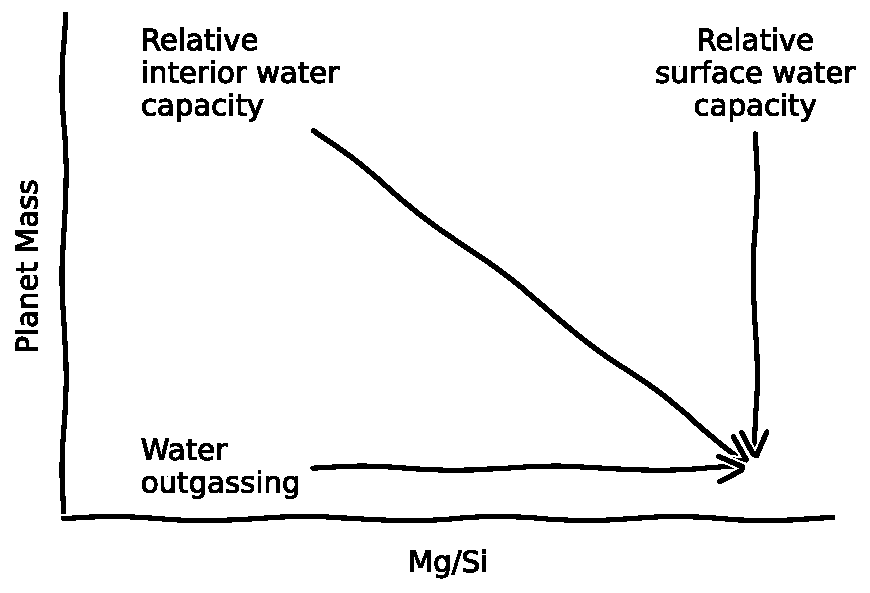
\includegraphics[width=0.66\linewidth]{summary}
\caption[Summary cartoon of water on rocky planets in the context of their mass and compositional diversity.]{Water on rocky planets contextualised within this thesis' overarching themes of planetary mass and compositional diversity. Arrows show proposed trends of increasing water content.}
\label{fig:surfacewater}
\end{figure}


%\todo{show plot with water and topography --- but what are the limits to predicting surface water? not just modelling outgassing because the atmosphere is really important. cf. Ana Lobo paper, yoshi miyazaki stuff... won't just condense into an ocean reliably}


The classic definition of planetary habitabilty is based on the stability of liquid water \citep{kasting_habitable_1993}. Much of the work presented in this thesis is, indirectly or directly and not-entirely-by-accident, related to where a planet's water is. It might therefore be interesting to place the preceding chapters in a retrospective watery framework. Here we can adopt the paradigm that virtually all of a rocky planet's total water mass will be partitioned between two reservoirs, its surface oceans and its mantle. In Chapters \ref{chapter:topography} and \ref{chapter:rockywater}, I predicted the capacity of these reservoirs respectively. In Chapter \ref{chapter:outgassing}, I predicted the flux of water between them, under certain conditions. Finally, in Chapter \ref{chapter:fo2}, I put constraints on the distribution of the most influential single parameter (cf. Fig. \ref{fig:corr}) affecting this flux; that is, \fo. Taking the results of these works together within the two main axes of rocky planet diversity introduced in Chapter \ref{chapter:intro}, some general trends in planetary water contents might be proposed (Fig. \ref{fig:surfacewater}).


With that said, I should stress that these four studies were not designed to be cognitively coupled in this way; i.e., to make rigorous predictions about how water flows through and on top of planets in general. Importantly, the actual presence of surface water on a planet is not guaranteed, even if the planet is in the circumstellar habitable zone of water stability, and even if it is endowed with water from formation. Whether or not a rocky planet can ultimately build and maintain surface oceans will be determined by its instantaneous atmospheric conditions as much as its interior conditions. For example, a certain minimum atmospheric partial pressure of water vapour is needed if water condensation is to proceed at all, which depends on the surface temperature and \ce{CO2} partial pressure \citep{miyazaki_inefficient_2022, miyazaki_wet_2022}. Models of atmosphere dynamics have revealed complex patterns of surface water loss on rocky planets \citep[e.g.,][]{lobo_terminator_2023}; these processes may ultimately need to be considered if we hope to make some predictions about planetary habitability, in this classical sense of the word. 


\section{Outlook}

\subsection{Parameter uncertainty}

All (exo)planetary interior modelling has been limited by the available data. There are three obvious areas where more or higher-quality data would directly advance our field.


\subsubsection{High-precision abundance measurements of planet-hosting stars and white dwarfs}


The uncertainty on stellar abundances is still too high to delimit individual exoplanets according to mineralogical ``populations''. This abundance data must be an order of magnitude more precise (1/1000 dex) if we are to make meaningful inferences about a given planet's mantle mineral modes \citep{hinkel_star_2018}. High-precision measurements of stellar Fe abundances are necessary to place upper limits on an exoplanet's metal core size, and therefore constrain its interior structure, maximum volatile-envelope mass fraction, and nominal likelihood of being rocky (\citealt{schulze_probability_2020, unterborn_nominal_2023}, cf. Fig. \ref{fig:compositional-link}). Lastly, a larger sample of high-precision abundances in polluted white dwarfs will be vital to test empirically how the refractory element ratios of planets are modulated from those of their host stars (cf. Fig. \ref{fig:hypatia_vs_pwd}): the omnipresent working hypothesis in all studies of rocky planet interior compositions. 


As I discussed in Chapter \ref{chapter:intro}, much of the error on FGKM star abundances is due to different data reduction techniques between researchers, as opposed to actual measurement error introduced by our instrumentation. The observational astrophysics community is making efforts to understand why this disagreement exists, and to find steps to minimise it \citep{hinkel_comparison_2016}. Notably, individual groups have been reporting abundances at this precision for nearly a decade \citep[e.g.,][]{ramirez_chemical_2014, nissen_highprecision_2015, spina_planet_2016}; it does not seem impossible to achieve more widely in the near future. Any interpretation of the white dwarf data hinges on our theoretical understanding of these bodies' accretion dynamics, but this is an area of active research \citep[e.g.,][]{harrison_bayesian_2021, buchan_planets_2022, brouwers_asynchronous_2022, brouwers_asynchronous_2023}.


\subsubsection{High-pressure mineral data}

We do not understand the behaviour of minerals at high mantle pressures perhaps as well as we would like to. Predictions of the interior structures of massive rocky planets are limited by uncertainties in the equations of state parameters and phase equilibria of silicates, especially above $\gtrsim$0.5 TPa. However, even if the highest pressures are a challenge to reach in laboratory settings, first-principles methods (e.g., density functional theory) have already proven vital in data generation \citep[e.g.,][]{umemoto_twostage_2011, tackley_mantle_2013, sakai_experimental_2016, umemoto_phase_2017}. %das_highpressure_2020, kovacevic_miscibility_2022, li_ultrahighpressure_2022}.


Beyond equations of state, it is also necessary that we constrain other material properties relevant for mantle thermal evolution: namely, viscosities and melting temperatures. These data are incomplete across exoplanet parameter space even at lower pressures, since most experimental petrology work so far has not necessarily needed to perform measurements across extraterrestrial mantle compositions. Even a null result (i.e., a negligible dependence) would be immensely useful. A systematic effect of Mg/Si on viscosity, assuming one can be found, could easily be adopted into convection models \citep{spaargaren_influence_2020}---this example is salient because planetary Mg/Si distributions might be measureable.

For example, where Chapter \ref{chapter:rockywater} adopted certain fiducial values of the water capacities of perovskite, stishovite, davemaoite, postperovskite \textit{etc.}, with better data in the future I anticipate that these results will be revised. In particular, the pressure-dependence of these phases' water capacities needs to be determined. \citet{deng_water_2022}, in a conference proceeding, present preliminary calculations of the water capacity of bridgmanite using molecular dynamics simulations and machine learning, the formal publication of which I am currently awaiting.




% although this has so far not succeeded, this could provide agreed-upon parameters that go into viscosity laws for a mantle in terms of temperature, pressure, mg/si, and water content




\subsubsection{The surface composition of Venus}

The solar system has another Earth-mass planet. Yet apart from the obviously hellish climate, we know hardly anything about its geology. Previous observations of our sister planet's surface emissivity have appeared consistent with felsic crustal rocks, which, intriguingly, would crystallise in the presence of water similar to Earth's granite continents \citep{hashimoto_felsic_2008}. Planned space missions VERITAS and EnVision (set with 2030s launch dates if not indefinitely delayed) would finally map the surface mineralogy of Venus. Given that Venus' bulk mantle mineralogy is expected to be very similar to Earth's, understanding how different the derived crusts are between the two planets would be an invaluable data point, if we are to ever understand the range of crustal compositions of exoplanets. These missions would also provide needed insight into Venus' enigmatic tectonic style, aiding our confidence in modelling the thermal histories of Venus-like exoplanets. 

As a note, the existence of Venus proves that planets are not pushed down pre-determined evolutionary tracks according to their position in Mg/Si--$M_p$ parameter space. The major question, ``why are Venus and Earth different today?'', would not have a simple answer, but any progress towards it is progress towards understanding planets.


\nomenclature[z-v]{VERITAS}{Venus Emissivity, Radio science, InSAR, Topography, And Spectroscopy}

\subsection{Model uncertainty}


Apart from minimising uncertainty on the input data, the other direction for future work attends to the infrastructure of models itself. Fast, simple 1D thermal history models are probably our best tool for exploring exoplanet parameter space. However, these models must capture the necessary physics. Sometimes higher-resolution 2D or 3D models can find certain insights into nonlinear processes that 1D models cannot. Melting rate estimates are a special challenge in 1D due to this nonlinearity (e.g., local melting depends on the history of previous melting, Chapter \ref{chapter:outgassing}; see also a review by \citealt{katz_physics_2022}). As such, a useful calculation would be to quantify the discrepancy in absolute melt volumes between high-resolution numerical models \citep[e.g.,][]{noack_volcanism_2017} and contemporary 1D models \citep[e.g.,][]{spaargaren_influence_2020, baumeister_redox_2023}, all else equal. I note that there are some good parameterisations of mantle melting in existence \citep[e.g.,][]{katz_new_2003}, but seemingly no unified method for applying them at planetary scales. Previous 1D studies of exoplanet mantle outgassing \citep[e.g.,][]{liggins_growth_2022} have plugged in constant values of numerically-calculated planetary melting rates from the literature, but by nature this approach cannot capture time-dependence or nonlinearity \citep[cf.][]{keller_statistical_2012}, and are of course stuck in nominal tectonic regimes, compositionally-dependent rheologies and solidii, \textit{etc}. 

Nevertheless, fully-coupled 1D thermal history models, which track water dynamics and their effects on mantle melting and viscosity, have demonstrated recent success resolving some old issues about Earth's thermal history \citep{seales_buffering_2022}. Thus, if we have melting implementations we can believe in, especially now that initial conditions for mantle water content are offered (Chapter \ref{chapter:rockywater}), we might apply 1D models of mantle convection to put realistic constraints on the expected range of---as per a theme of this thesis---\ce{H2O} outgassing fluxes on rocky planets, as a function of their (observeable) mass, age, and host star composition. Fluxes of \ce{CO2} are a natural extension \citep[see][]{lehmer_carbonatesilicate_2020}, being a key hurdle in predicting the climate states of planets in the circumstellar habitable zone \citep[e.g.,][]{graham_co2_2022}, although the geochemistry governing carbon's storage and transport in the mantle is distinct from that of water \citep{dasgupta_ingassing_2013}. From there we can address the expected variety of planetary climates within the circumstellar habitable zone, naturally feeding estimations of the frequency of truly Earth-like planets, laying the groundwork for a statistical understanding of Earth’s cosmic station.




%\todo{coupled 1D models involving water transport, its effects on melting and viscosity, have demonstrated recent success in possibly resolving some old issues about earth's thermal history \citep{seales_buffering_2022}, and these considerations are simple enough and clearly justified to go into future 1D thermal models for exoplanets, now that I have provided initial conditions }


%\todo{in need of new scaling laws for melting rates, or a distribution of melting rates, that can slot into parameterised models, in particular of stagnant lid planets. these could be obtained from numerical experiments }




%TTFN!



% ********************************** Back Matter *******************************
% Backmatter should be commented out, if you are using appendices after References
%\backmatter

% ********************************** Bibliography ******************************
\begin{spacing}{0.9}

% To use the conventional natbib style referencing
% Bibliography style previews: http://nodonn.tipido.net/bibstyle.php
% Reference styles: http://sites.stat.psu.edu/~surajit/present/bib.htm

\bibliographystyle{apalike}
%\bibliographystyle{unsrt} % Use for unsorted references  
%\bibliographystyle{plainnat} % use this to have URLs listed in References
\cleardoublepage
\bibliography{References/exogeodynamics} % Path to your References.bib file


% If you would like to use BibLaTeX for your references, pass `custombib' as
% an option in the document class. The location of 'reference.bib' should be
% specified in the preamble.tex file in the custombib section.
% Comment out the lines related to natbib above and uncomment the following line.

%\printbibliography[heading=bibintoc, title={References}]


\end{spacing}

% ********************************** Appendices ********************************

\begin{appendices} % Using appendices environment for more functunality

%!TEX root = ../thesis.tex
% ******************************* Thesis Appendix A ****************************
\chapter{Spherical harmonic methods for topography} 
\label{sec:sph-harms}

\ifpdf
    \graphicspath{{Chapter1/Figs/Raster/}{Chapter1/Figs/PDF/}{Chapter1/Figs/}}
\else
    \graphicspath{{Chapter1/Figs/Vector/}{Chapter1/Figs/}}
\fi


\begin{figure}
    \centering
    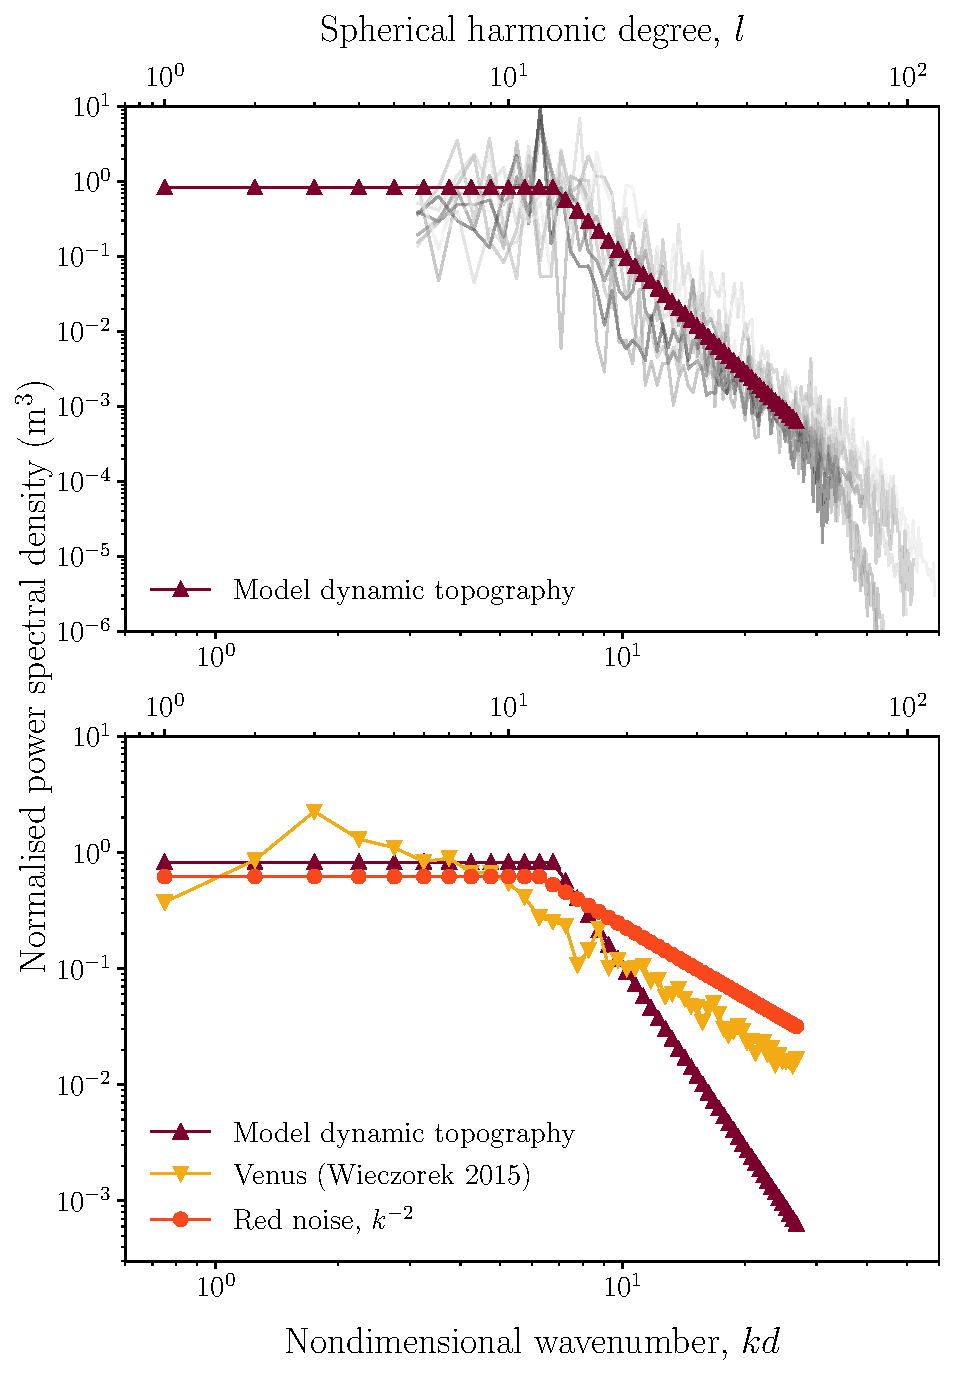
\includegraphics[width=0.8\textwidth]{psd_stacked_k.pdf}
    \caption[Dimensionless 1D power spectral densities of dynamic topography.]{\textit{(Top:)} Dimensionless 1D power spectral densities of dynamic topography from 2D numerical convection simulations, normalised to an RMS power of unity. In purple triangles is the model dynamic topography spectrum obtained from a log-linear fit to the Ra$_1 = 10^8, \Delta \eta = 10^7$ case. \textit{(Bottom:)} The model dynamic topography spectrum shown with, in yellow triangles, the observed overall topography of Venus \citep{wieczorek_gravity_2015}, and, in red circles, a theoretical spectrum with a power-law dependence $\propto k^{-2}$, corresponding to red noise.
    \label{fig:top-spectra}}
\end{figure}



\section*{A baseline power spectrum} \label{sec:spectral-model}

We choose our Case 4 simulation (Table \ref{tab:aspect}) from which to extract a scaleable model spectrum of the surface dynamic topography, since its temporal distribution of $h_{\rm rms}^\prime$ is the most narrow. A type-2 orthonormalised discrete cosine transform of this profile produces a Fourier representation,
\begin{align}
    \begin{split}
    f_p &= 2 \gamma \sum_{n=0}^{N-1} h_n^\prime \cos \left( \frac{\pi p (2n + 1)}{2N}\right),\\
    \gamma &= 
    \begin{cases}
      \sqrt{\frac{1}{4N}}, & \text{if}\ p=0 \\
      \sqrt{\frac{1}{2N}}, & \text{otherwise,}
    \end{cases}
\end{split}
\end{align}
from which we can find a 1D power spectral density,
\begin{equation}
    \phi^{\rm 1D}_0 = 2 \Delta x^\prime \left(f_p\right)^2,
\end{equation}
as a function of dimensionless wavenumber,
\begin{equation}
    k^\prime = \frac{\pi}{L^\prime} p,
\end{equation}
where $h_n^\prime$ is the height of dynamic topography at sample point $n$, $N$ is the number of sample points in the spatial profile (fixed by the mesh size), $p = [0, ..., N - 1]$, $L^\prime = 8$ is the dimensionless box width, and $\Delta x^\prime = L^\prime / N$. We calculate $\phi^{\rm 1D}_0$ at every model time step and use the average for our baseline spectrum. This spectrum has an RMS amplitude $h^{\prime}_{\rm rms, 0}$. 

There is an upper wavenumber limit, $k^\prime_{\rm max}$, at around the equivalent wavelength of the upper thermal boundary layer thickness, $\delta_{\rm rh}$, where features narrower than this are not meaningful for the dynamic topography. We also observe all spectra roughly rolling off to a constant value at wavenumbers below around twice the convection cell depth, so we set $k_{\rm min}^\prime = 2d$. In log-log space, $\phi^{\rm 1D}_0$ is approximately linear from $k_{\rm min}^\prime$ to $k^\prime_{\rm max}$. Therefore we approximate the power spectra by two line segments. We fit a constant slope between $k^\prime_{\rm min}$ and $k^\prime_{\rm max}$, and assign a value of $\phi^{1D}_0(k^\prime_{\rm min})$ wherever $k^\prime < k^\prime_{\rm min}$. This fit is done to the average power spectral density over all time steps for the given simulation. We interpolate this fitted function such that it has a discrete value at each integer spherical harmonic degree $l$, where $l = k^\prime R_p^\prime - 0.5$, from $l=1$ to the nearest degree to $k^\prime_{\rm max}$. That is, we do not scale $k^\prime_{\rm max}$. Whilst realistically $k^\prime_{\rm max}$ would increase with Ra$_1$, the effect on $h_{\rm rms}^\prime$ is small (less than one part in a thousand) because these high wavenumber bands hold such little relative power. For this generic spectrum we assume a dimensionless planet radius $R_p^\prime = 2$ (a core radius fraction of 0.5 for a dimensionless mantle depth of 1; varying $R_p^\prime$ has negligible effects on the results).


Figure \ref{fig:top-spectra} shows the 1D power spectral densities $\phi^{\rm PSD}_h$ of dynamic topography computed from our 2D numerical modelling experiments, normalised as a percentage of the total power. Between $k_{\rm min}^\prime$ and $k_{\rm max}^\prime$, the log-linear slopes of the topography spectra are roughly similar within the noise for all Ra$_1$, $\Delta \eta$ cases. Due to our limited number of 2D runs, however, we cannot really make a compelling case for this statement, and we would not back our interim result outside of its intended, rather inconsequential usage here. For example, we might expect more vigorous, higher-Ra convection to exhibit more smaller-scale drips from the upper thermal boundary layer, leading to slightly more topographic power at high wavenumbers---although the total power would be virtually unaffected by these high-frequency features. Note also that because the spatial domain topography is 1D, data paucity will always entail a certain amount of noise, compared to a 2D grid of topography from a 3D convection simulation.

Also in figure \ref{fig:top-spectra} is the observed topography spectrum of Venus from \citet{wieczorek_gravity_2015}. On Venus, elastic and compositional sources of topography are superimposed upon dynamic topography. Venus' spectrum thus provides an empirical modification of the pure dynamic topography. As a third and final spectral model, we have the theoretical red noise spectrum given by the power law $\phi^{\rm PSD}_h \propto k^{-2}$ and a roll-off wavenumber the same as the numerical spectrum. Compared to the numerical dynamic topography, Venusian topography and red noise topography both have a shallower slope and retain more power at higher wavenumbers---as expected from the high-frequency nature of topography created by impact cratering and volcanism. The Venus spectrum additionally shows a peak at degree $l=3$. Note that these (normalised) spectra represent different geophysical and geomorphologic processes, and are therefore not expected to have the same absolute RMS value.


\section*{Generating random maps} \label{sec:spectral-repeat-top}


\begin{figure}
    \centering
    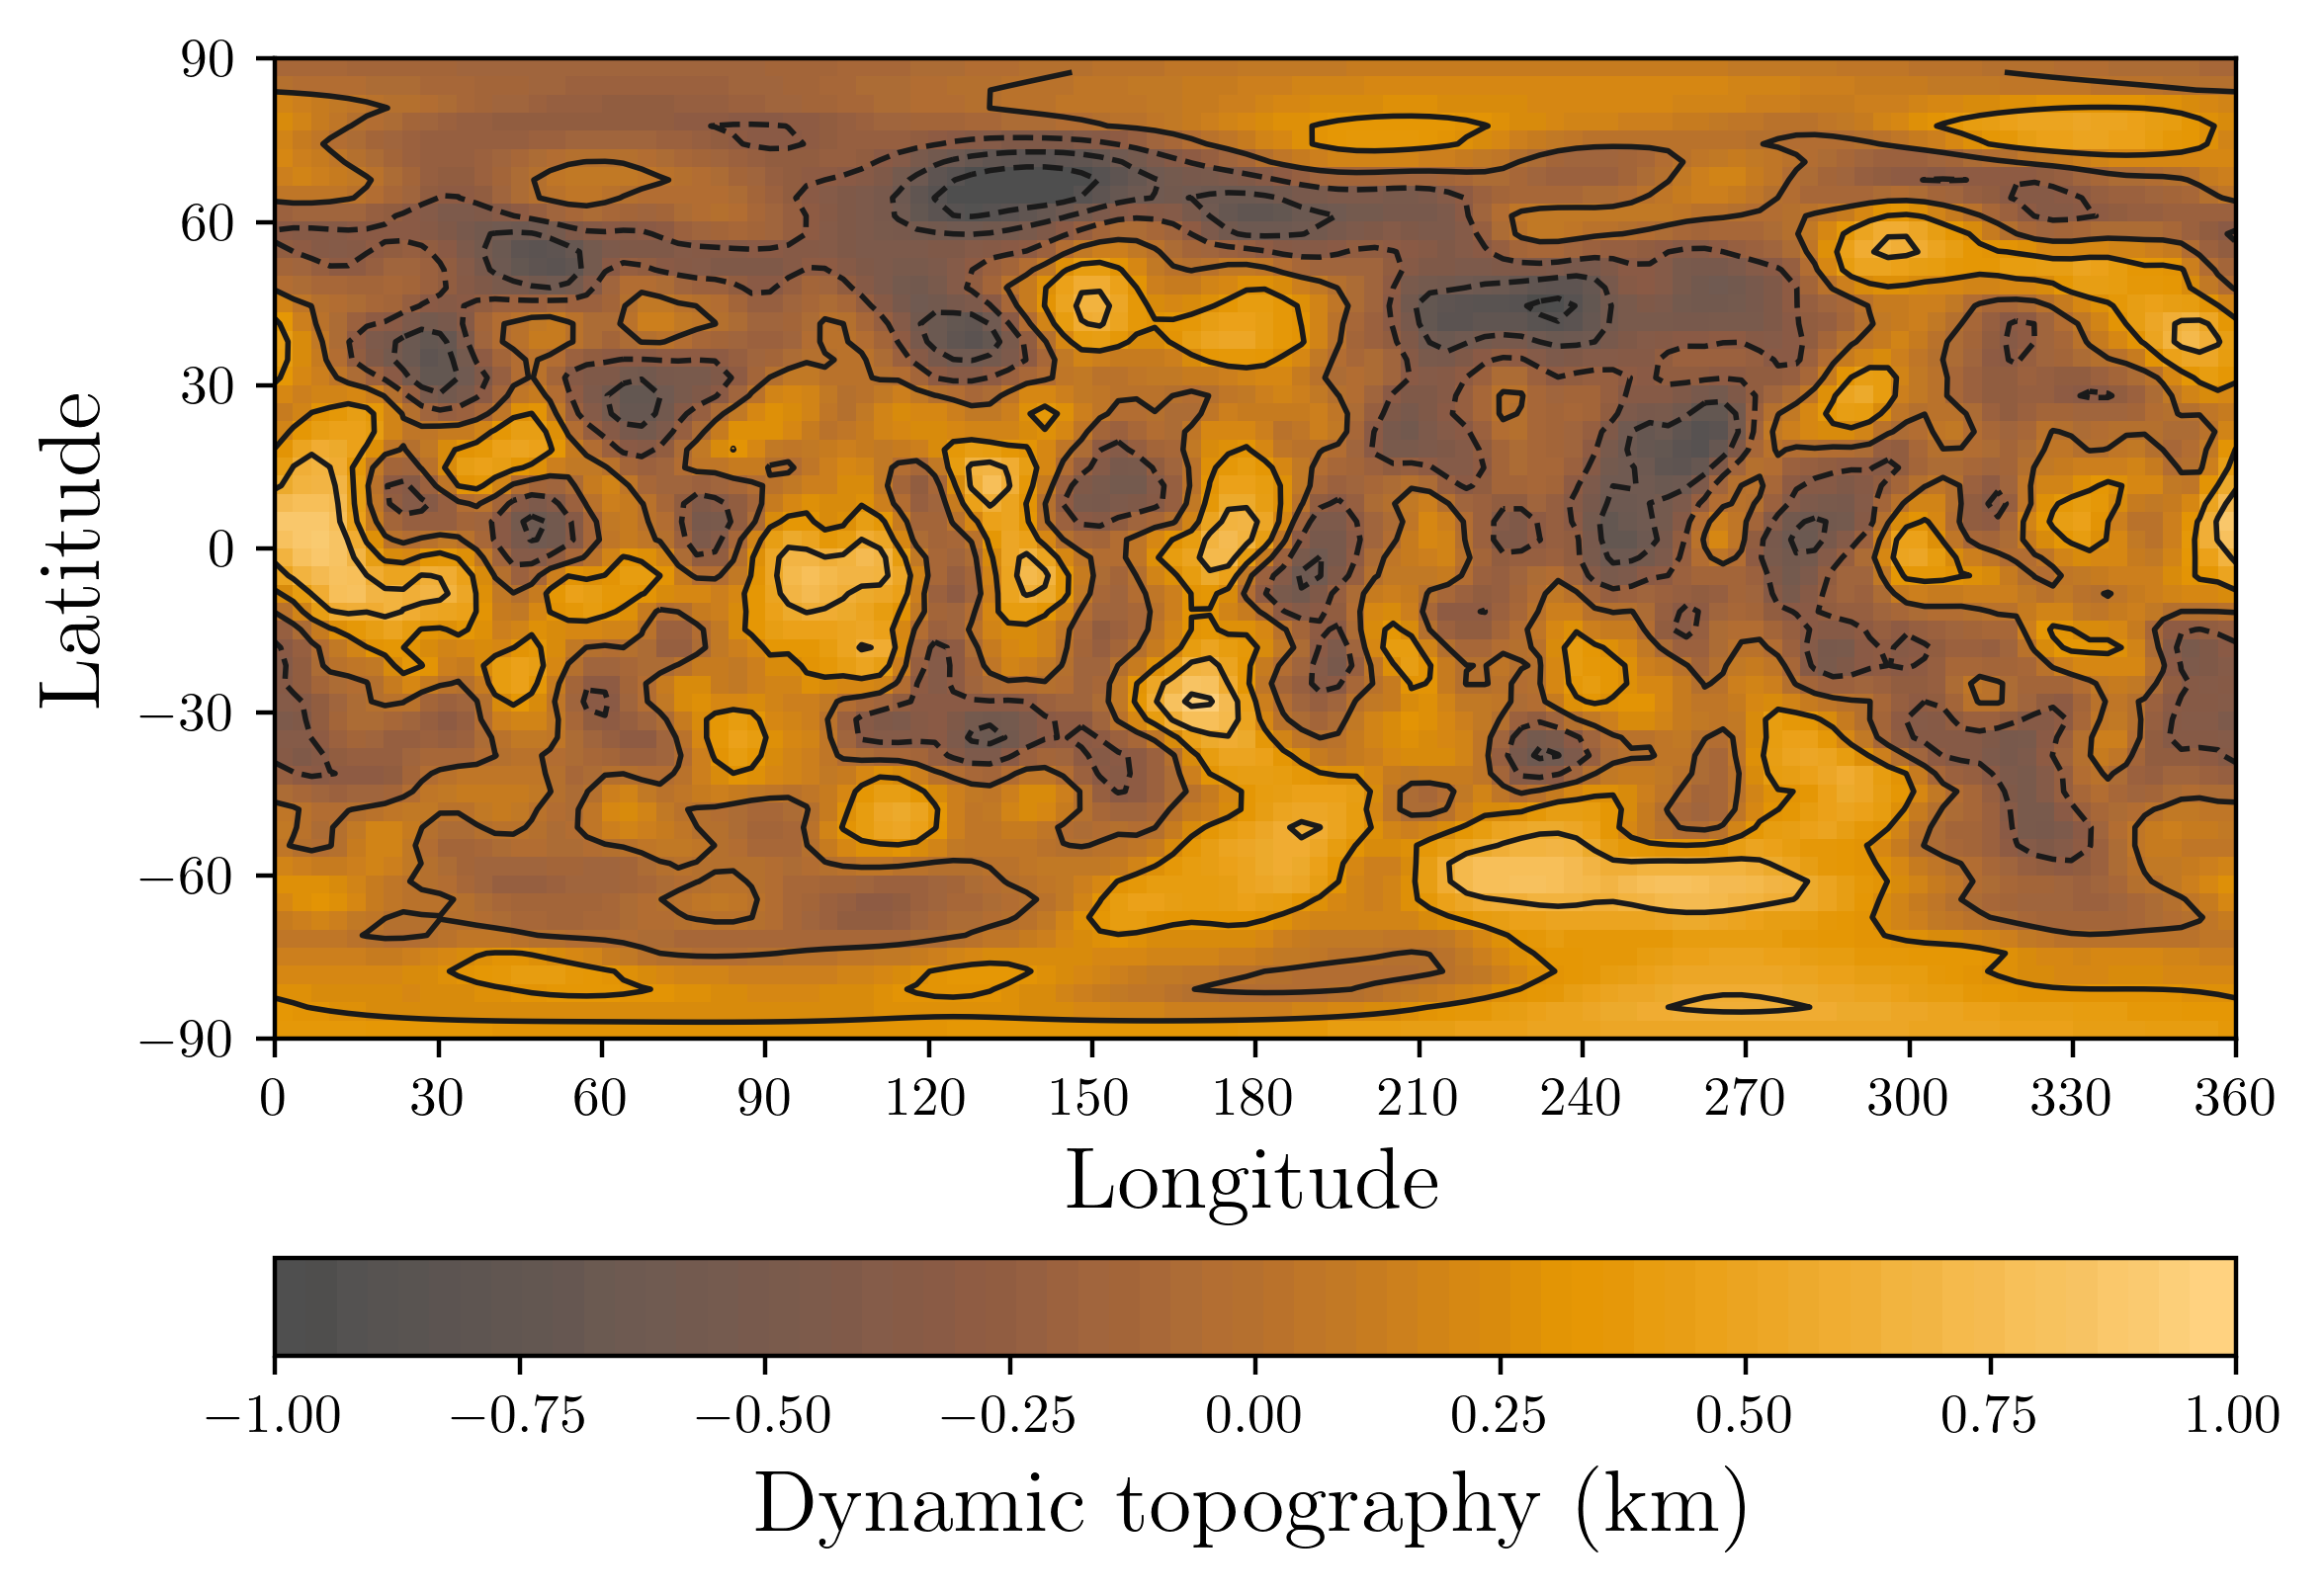
\includegraphics[width=0.7\textwidth]{topo_grid.png}
    \caption[An example of a synthetic topography map of an exoplanet, obtained by expanding a realistic power spectrum.]{A synthetic topography map, obtained from a random power spectrum ($l_{\rm max} = 53$) consistent with the numerically-modelled ``baseline" dynamic topography spectrum (see text for details on randomisation). This map has a peak elevation of 820 m and an RMS elevation of 190 m. The nominal planet has a mass of 1~$M_\oplus$, dry olivine rheology, and a solar radiogenic heating budget.
    \label{fig:synth-map}}
\end{figure}

We use the {\tt pyshtools.SHCoeffs.from{\_}random()} function to obtain a set of spherical harmonic coefficients consistent with $\phi^{1D}_0$ \citep{wieczorek_shtools_2018}. This function requires a power per $l$ (dimensional units m$^2$), so we apply a conversion from $\phi^{1D}_0$ (dimensional units $\rm{m^2\,m}$). First we find the effective 2D power spectral density assuming radial symmetry, $\phi^{2D}_{\rm iso}$ (dimensional units $\rm{m^2\,m^2}$), which would correspond to our 1D spectrum:
\begin{equation}
\phi^{2D}_{\rm iso} = \frac{1}{k^\prime} \phi^{1D}_0.
\end{equation}
The power per $l$ is:
\begin{equation}
S_l = \frac{\phi^{2D}_{\rm iso} \left(2 l + 1\right)}{4 \pi R_p^{\prime 2}}.
\end{equation}
With these normalisations, the total power per coefficient,
\begin{equation}
S_{lm} = \frac{S_l}{2l + 1},
\end{equation}
is proportional to $\phi^{2D}_{\rm iso}$. In converting our spectra into 2D equivalents, we are presupposing that 2D Cartesian and 3D spherical models result in approximately similar topography power spectra with consistent $h_{\rm rms}^\prime$. Using the output from \citet{lees_gravity_2020}, we have verified that constant-viscosity convection in Cartesian geometry indeed produces similar spectra between 2D and 3D, but the assumption remains a caveat until dedicated 3D spherical realisations can test it. Nevertheless, we already know that it is incorrect to try fitting a scaling function to 2D numerical $h_{\rm peak}$ directly---this quantity is certainly sensitive to details of the model setup, as we have mentioned in section \ref{sec:methods-hscaling}.

If we are seeking a spatial map of a hypothetical spectrum other than $\phi^{1D}_0$ (i.e., different RMS value), we take advantage of the fact that numerical dynamic topography spectra will appear to have roughly consistent slopes between $k^\prime_{\rm min}$ and $k^\prime_{\rm max}$, and hence scale $S_l$ appropriately, 
\begin{equation}
\bar{S_l} = S_l \left(\frac{h^{\prime}_{{\rm rms}, 1}}{h^\prime_{{\rm rms}, 0}}\right)^2,
\end{equation}
where $h^{\prime}_{{\rm rms}, 1}$ refers to the desired rms of the new spectrum. 

We can now obtain our set of coefficients via {\tt pyshtools}: %As a a test, we can look at the power per $l$, $S_l^{\rm rand}$ and power per $lm$, $S_{lm}^{\rm rand}$ of these coefficients using the {\tt spectrum(unit)} function from the {\tt pyshtools.SHCoeffs} class.
random spherical harmonic coefficients are generated from a normal distribution with unit variance, subject to the strong assumption of no correlation between wavenumbers. 
%We expect that the new, randomised power per coefficient $S_{lm}^{\rm rand}$ is equal to $\phi^{2D}_{iso}$ and, by Parseval's theorem,
% \begin{equation} \label{eq:rand_rms_check}
% \frac{1}{2\pi}\int\left(4 \pi R_p^{\prime 2} S_{lm}^{\rm rand} k^\prime \; \rm{d}k^\prime \right) \approx \left(h^{\prime}_{{\rm rms}, 1}\right)^2.
% \end{equation}


% \subsection{2D grid expansion and integration} 

Then we again use {\tt pyshtools} to expand the random spherical harmonic coefficients onto a Gauss-Legendre quadrature grid.
%regular grid of latitude and longitude (each cell being a square 0.743\degree wide). The rms of this topography grid is approximately equal to the desired $h^{\prime}_{{\rm rms}, 1}$.
% the total power of $S_{lm}^{\rm rand}$ by Parseval's theorem.
% \begin{equation}
% \frac{\sum h^2}{ N_{\rm cells}} \approx \frac{1}{4\pi^2}\int\left(4 \pi R^2 S_{lm}^{\rm rand} 2\pi k \; \rm{d}k \right).
% \end{equation}
At this stage we can dimensionalise the spatial domain topography with (\ref{eq:dimensionalise}), given the results of the parameterised convection model. A sample elevation map is shown in figure \ref{fig:synth-map}. %Because our purpose here entails that all land is underwater except for the single grid point corresponding to $h_{\rm peak}$, we scale the topography grid by a factor of $\rho_m/(\rho_m - \rho_w)$ (i.e., there is greater topography for the same amount of pressure difference).
% Finally, the ocean basin volume is found by integrating the expanded grid as in (\ref{eq:ocean-integral}), using the Gauss-Legendre quadrature rule.
% Finally, the ocean basin volume is the sum over all grid cells, $i, j$, of the volume bounded by the surface and the grid's maximum topography, $h_{\rm peak}$,
% \begin{equation}
%     V_{\rm ob} = \sum_{i} \sum_{j} \left( h_{\rm peak} - h_{ij} \right) A_{ij},
% \end{equation}
% where $A_{ij}$ is the area of the cell in m$^2$, calculated assuming that the planet is a perfect sphere. 
Because the randomly-generated spherical harmonic coefficients are not unique for a given power spectrum, we reduce the noise by generating 500 sets of coefficients and taking the average of the resulting peak elevation values.



%!TEX root = ../thesis.tex
% ******************************* Thesis Appendix B ********************************

\chapter{Supplementary Tables and Figures}

\ifpdf
    \graphicspath{{Appendix2/Figs/Raster/}{Appendix2/Figs/PDF/}{Appendix2/Figs/}}
\else
    \graphicspath{{Appendix2/Figs/Vector/}{Appendix2/Figs/}}
\fi



\tochide\section{Supplementary Tables for Chapter \ref{chapter:topography}}
\label{sec:aspect-table}

Table \ref{tab:aspect-out} provides additional numerical output from ASPECT. See section \ref{sec:methods-numerical} for definitions of these quantities. Nu is the Nusselt number, the ratio of convective to conductive heat transfer at the surface, calculated as ${\rm Nu} = Y^\prime F^\prime_0 / [k^\prime(T^\prime_1 - T^\prime_0)]$, where $Y^\prime$ is the dimensionless box height, $ F^\prime_0$ is the total surface dimensionless heat flux divided by the dimensionless box width, $k^\prime = 1$ is the dimensionless thermal conductivity, and $T^\prime_1$ and $T^\prime_0$ are the dimensionless temperatures at the bottom and top boundaries respectively.

\begin{table}[h!]
\centering
\caption{Selected time-averaged results of the numerical model. Symbols are defined in the text. \label{tab:aspect-out}}
\footnotesize
\begin{tabular}{@{} c r r r r r r r r r r r @{}}
\toprule
Case & Ra$_1$ & $\Delta \eta$ & Ra$_i$ & $D_{\rm lid}^\prime$ & $\delta_{\rm rh}^\prime$ & $T_i^\prime$ & $T_{\rm lid}^\prime$ & $\Delta T_{\rm rh}^\prime$ & Nu & $h_{\rm rms}^\prime$ & $h_{\rm peak}^\prime$  \\
\midrule

% copy from python
2 & $2 \times 10^{8}$ & $1 \times 10^{6}$ & $7.20 \times 10^{7}$ & $0.133$ & $0.0248$ & $0.926$ & $0.785$ & $0.141$ & $6.17$ & $0.00716$ & $0.0152$ \\
3 & $3 \times 10^{8}$ & $1 \times 10^{6}$ & $1.07 \times 10^{8}$ & $0.118$ & $0.0218$ & $0.925$ & $0.790$ & $0.135$ & $6.97$ & $0.00667$ & $0.0130$ \\
4 & $1 \times 10^{8}$ & $1 \times 10^{7}$ & $3.62 \times 10^{7}$ & $0.199$ & $0.0370$ & $0.937$ & $0.794$ & $0.143$ & $4.10$ & $0.00893$ & $0.0214$ \\
5 & $2 \times 10^{8}$ & $1 \times 10^{7}$ & $7.08 \times 10^{7}$ & $0.165$ & $0.0238$ & $0.936$ & $0.816$ & $0.120$ & $5.12$ & $0.00610$ & $0.0159$ \\
6 & $3 \times 10^{8}$ & $1 \times 10^{7}$ & $1.07 \times 10^{8}$ & $0.148$ & $0.0215$ & $0.936$ & $0.816$ & $0.120$ & $5.70$ & $0.00673$ & $0.0145$ \\
7 & $1 \times 10^{8}$ & $1 \times 10^{8}$ & $3.60 \times 10^{7}$ & $0.235$ & $0.0394$ & $0.945$ & $0.806$ & $0.138$ & $3.50$ & $0.00907$ & $0.0243$ \\
8 & $2 \times 10^{8}$ & $1 \times 10^{8}$ & $7.24 \times 10^{7}$ & $0.199$ & $0.0295$ & $0.945$ & $0.821$ & $0.124$ & $4.23$ & $0.00765$ & $0.0174$ \\
9 & $3 \times 10^{8}$ & $1 \times 10^{8}$ & $1.08 \times 10^{8}$ & $0.179$ & $0.0253$ & $0.945$ & $0.826$ & $0.118$ & $4.75$ & $0.00788$ & $0.0179$ \\
10 & $1 \times 10^{8}$ & $1 \times 10^{9}$ & $3.57 \times 10^{7}$ & $0.274$ & $0.0427$ & $0.950$ & $0.819$ & $0.131$ & $3.03$ & $0.00815$ & $0.0252$ \\
11 & $2 \times 10^{8}$ & $1 \times 10^{9}$ & $7.20 \times 10^{7}$ & $0.232$ & $0.0329$ & $0.951$ & $0.831$ & $0.120$ & $3.65$ & $0.00878$ & $0.0250$ \\
12 & $3 \times 10^{8}$ & $1 \times 10^{9}$ & $1.11 \times 10^{8}$ & $0.213$ & $0.0262$ & $0.952$ & $0.846$ & $0.105$ & $4.07$ & $0.00876$ & $0.0180$ \\





% end copy

\bottomrule
\end{tabular}
\end{table}


\clearpage

\begingroup
%  \makeatletter
%  \setlength{\chapter@bottom@space}{15pt}
%  \makeatother
%\titleformat{\chapter}[display]
%    {\normalfont\huge\bfseries}{\chaptertitlename\ \thechapter}{0pt}{\Huge}
\titlespacing*{\section}{0pt}{20pt}{70pt}  % left, upper, lower
%\let\LaTeXStandardClearpage\clearpage
%\let\clearpage\relax





\tochide\section{Supplementary Figures for Chapter \ref{chapter:rockywater}}
\label{sec:supp-rockywater}


\begin{figure}[!h]
         \centering
         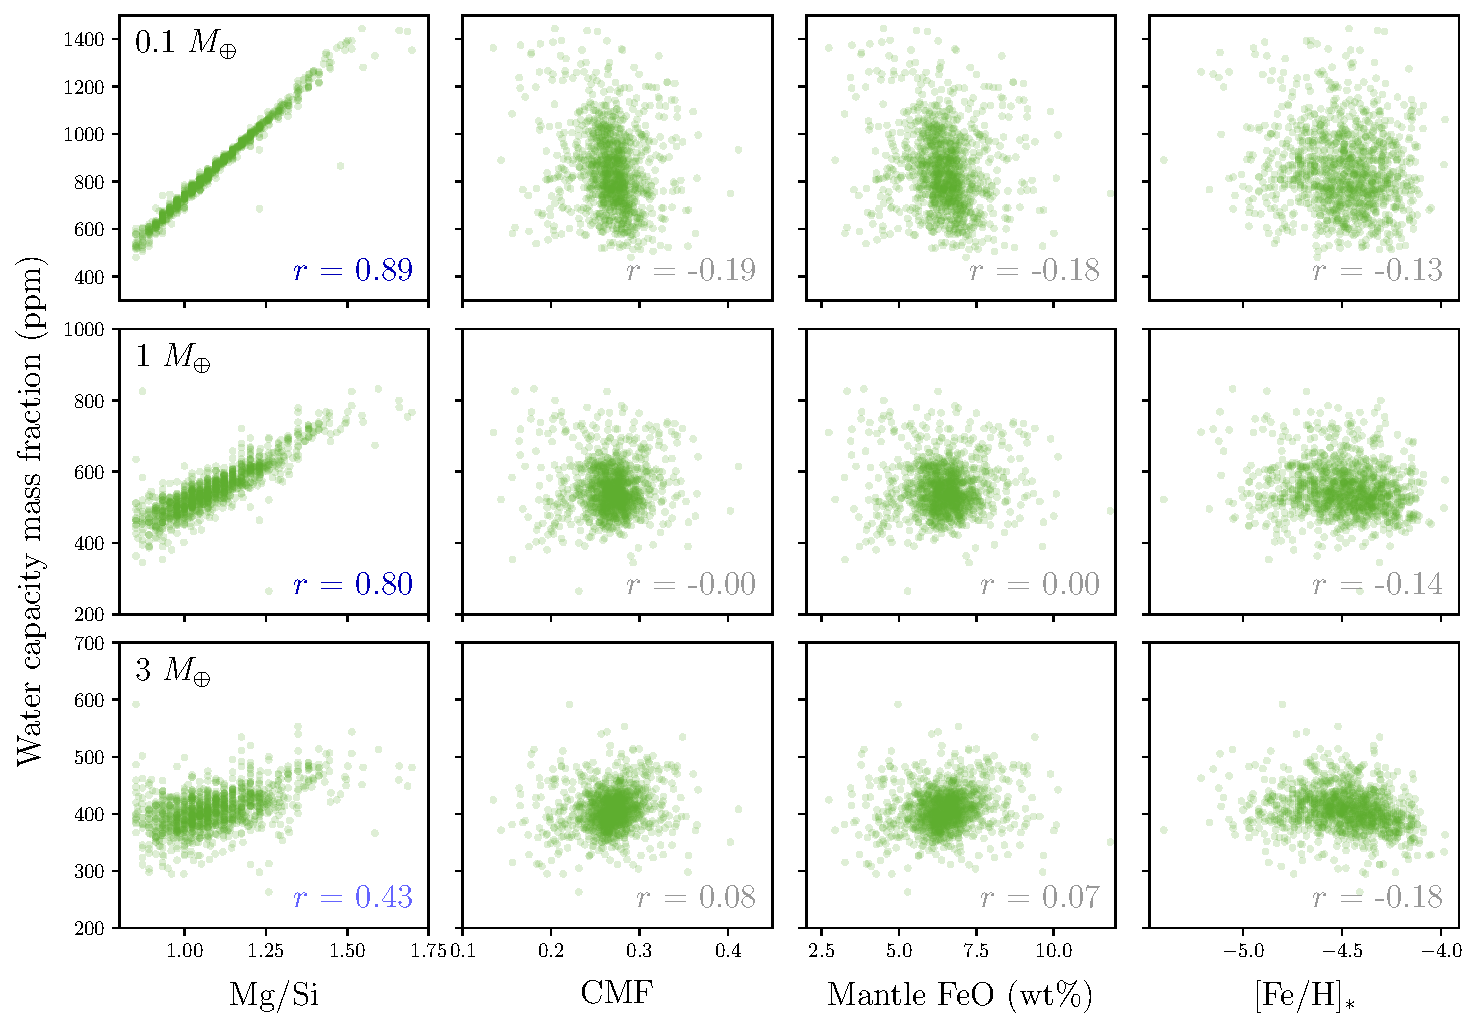
\includegraphics[width=\textwidth]{masses_spread.pdf}
        \caption[Cross plots of mantle water capacity with additional model parameters.]{Cross plots of water capacity (as a fraction of the planet mass), at 0.1 $M_\oplus$ \textit{(top row)}, 0.1 $M_\oplus$ \textit{(middle row)}, and 3 $M_\oplus$ \textit{(bottom row)}, in terms of, from left to right, the molar Mg/Si ratio of the bulk planet, the core mass fraction (CMF), the mantle FeO content in wt\%, and the host star's logarithmic number ratio of Fe to H. The bulk compositions sampled in this figure are based on all planet-hosting stars in the Hypatia Catalog, excepting low Mg/Si compositions for clarity. All planets are simulated with a constant mantle/core molar Fe partitioning of 0.113 and a potential temperature of 1600 K. The value of the Pearson's correlation coefficient $r$ is given in the bottom right corner of each panel. Water capacities correlate significantly only with Mg/Si; there is a high positive correlation for the 0.1 and 1 $M_\oplus$ cases, and a low positive correlation for the 3 $M_\oplus$ cases.}
        \label{fig:wmf_scatter}
\end{figure}


\begin{figure}[!h]
\centering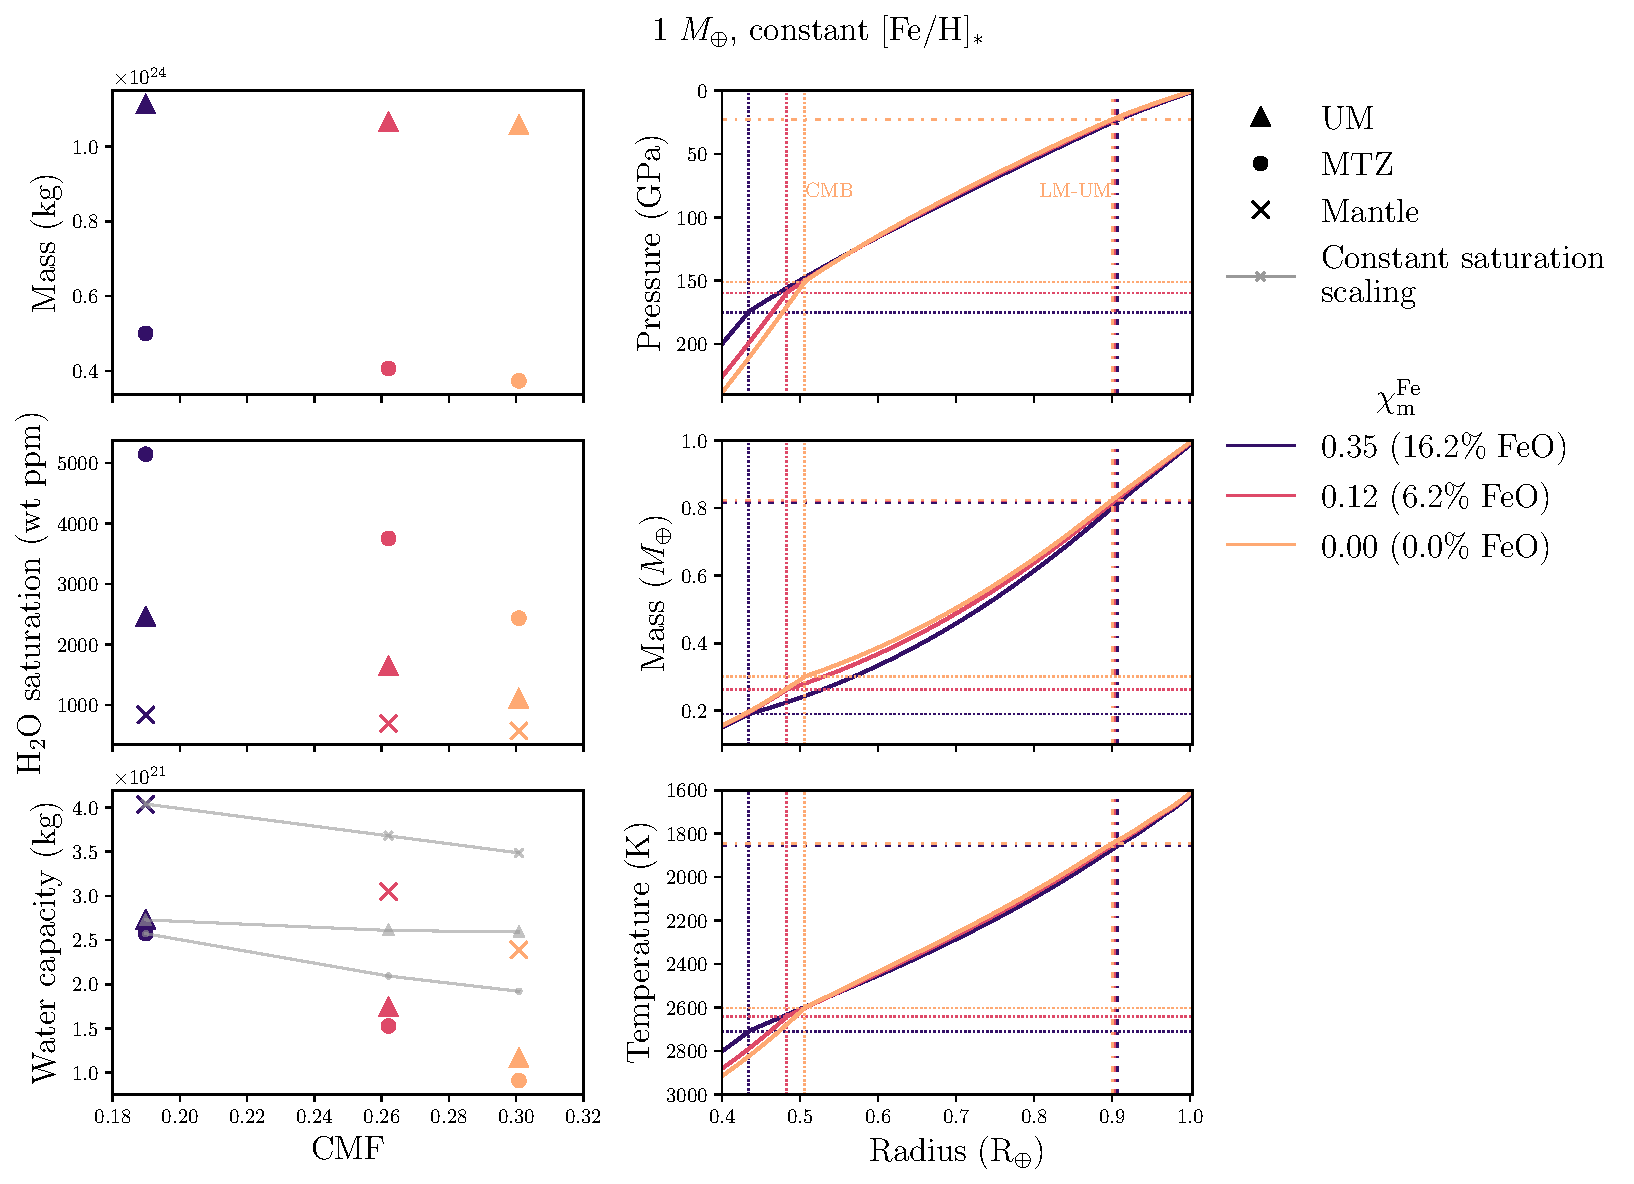
\includegraphics[width=\textwidth]{1M_structure_vs_CMF_coreeff.pdf}
\caption[The effect on mantle water capacity of pressure gradients due to varying the molar fraction of Fe in the mantle.]{The effect on mantle water capacity of pressure gradients due to planet chemistry. Here we fix the host star and planet's bulk abundance of Fe, [Fe/H]$_*$, but vary molar fraction of Fe in the mantle, $\chi^{\rm Fe}_{\rm m}$. The left column shows, from top to bottom, the layer masses, total water concentrations at water saturation with respect to the layer mass, and water capacities, as a function of the resulting core mass fraction (CMF), for the upper mantle (UM; triangles), mantle transition zone (MTZ; circles), and whole mantle (crosses). In the bottom left panel, the grey lines show the water capacities in kg if mineral water saturations were constant (arbitrarily at the value associated with the lowest CMF), and the only factors affecting water capacities were the masses of the layers. The right column shows, from top to bottom, the profiles of pressure, mass, and temperature through the mantle, with vertical and horizontal lines locating the core-mantle boundary (CMB; dotted lines) and the top of the lower mantle (LM-UM; dash-dotted lines). All cases are fixed to a planet mass of 1 $M_\oplus$ and a potential temperature of 1600 K. In the case of variable $\chi^{\rm Fe}_{\rm m}$, moving iron from the core to the mantle has a small positive effect on the mass of the upper mantle, and a larger positive effect on the mineral water saturation contents, which both act to increase the water capacity.}
\label{fig:pressure_gradients_coreeff}
\end{figure}


\begin{figure}
         \centering
         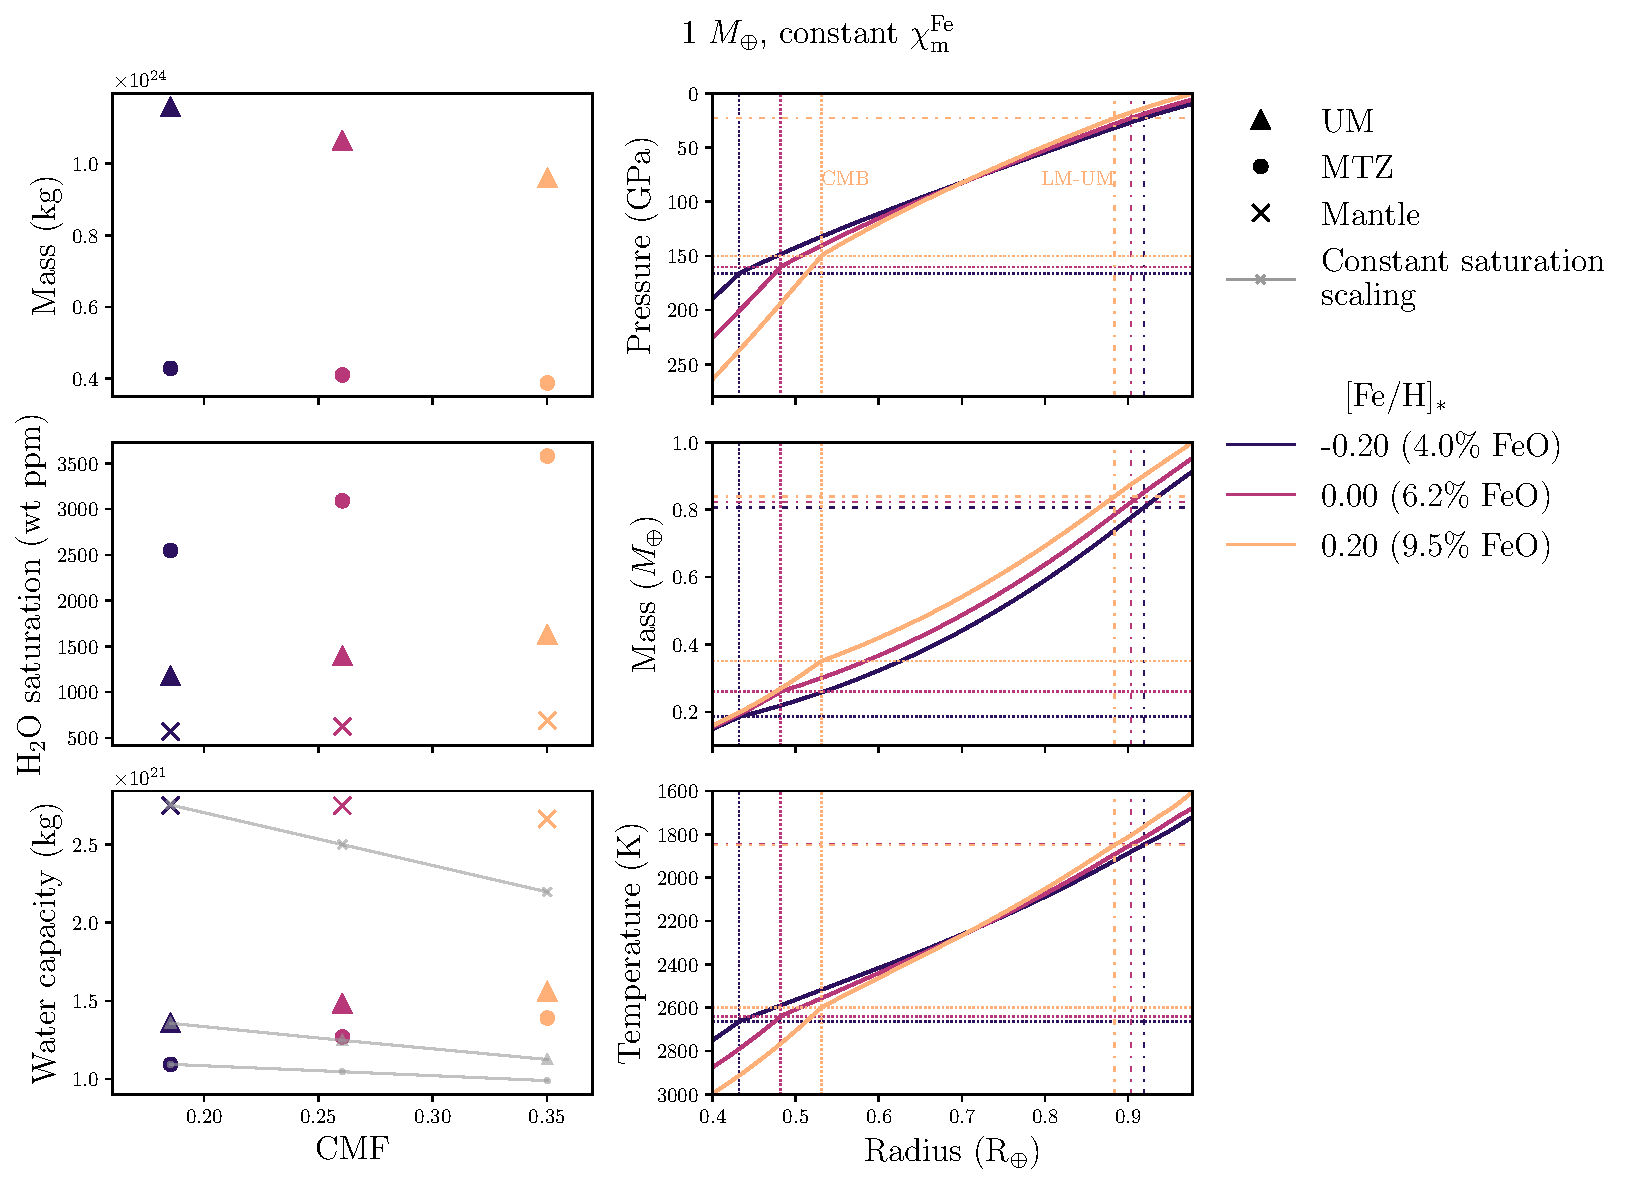
\includegraphics[width=\textwidth]{1M_structure_vs_CMF_feh.pdf}
         \caption[The effect on mantle water capacity of pressure gradients due varying the stellar Fe abundance.]{The same as in Fig. \ref{fig:pressure_gradients_coreeff}, but for a fixed planetary Fe partitioning, $\chi^{\rm Fe}_{\rm m}$, and variable stellar Fe abundance, [Fe/H]$_*$. In the case of variable [Fe/H]$_*$, increasing the overall iron content of the system has a negative effect on the mass of the upper mantle, and a positive effect on the mineral water saturation contents, the results of which nearly cancel out.}
        \label{fig:pressure_gradients_feh}
\end{figure}


\clearpage


\tochide\section{Supplementary Figures for Chapter \ref{chapter:fo2}}
\label{sec:supp-fo2}


\begin{figure}[!htb]
         \centering
\includegraphics[width=0.8\textwidth]{crossplot_mgsi_fit.png}
        \caption[Linear regression fit of mantle oxygen fugacity with Mg/Si ratio.]{The same cross-plots as the left columns of Figs. \ref{fig:xplots_mlts} and \ref{fig:xplots_px} in the main text but with linear regressions overlain in green: mantle oxygen fugacity, expressed as $\Delta$FMQ, as a function of the mantle molar Mg/Si ratio. Outliers (grey crosses), as determined by their effects on $\chi^2$ using a leave-one-out method, are excluded from the regressions. Slopes $m$ of the regressions are shown in the bottom right corner of each panel. Calculations are performed at $1373\,\text{K}$ and at $1\,{\rm GPa}$ \textit{(top)} and $4\,{\rm GPa}$ \textit{(bottom)}, using pMELTS \textit{(left)} and the \citet{jennings_simple_2015} database in Perple\_X \textit{(right)}. Each point represents a bulk mantle composition estimated from refractory element abundances of planet-hosting stars in the Hypatia Catalog \citep{hinkel_stellar_2014}.\label{fig:mgsi_fit}}
\end{figure}
\begin{figure}[!htb]
         \centering
\bigskip
\includegraphics[width=0.7\textwidth]{crossplot_al_opx.pdf}
        \caption[Modality ratios of spinel and garnet to orthopyroxene, as a function of Al/Si.]{Cross plot of the wt.\% modality ratios of an aluminous phase (spinel, Sp, or garnet, Gt) to orthopyroxene (Opx), as a function of the molar Al/Si ratio, estimated for rocky exoplanet mantles and based on refractory element abundances from planet-hosting stars in the Hypatia Catalog \citep{hinkel_stellar_2014}, here assuming an Earth-like molar ratio of core Fe-metal to mantle FeO. Calculations are performed at $1373\,\text{K}$ and at $1\,{\rm GPa}$, nominally the spinel field \textit{(top)}, or $4\,{\rm GPa}$, nominally the garnet field \textit{(bottom)}, using pMELTS \textit{(left)} and the \citet{jennings_simple_2015} database in Perple\_X \textit{(right)}. Note a few extreme cases are not visible in these $y$-axis limits. With increasing Al/Si, higher proportions of the aluminous phase are stabilised at the expense of orthopyroxene.\label{fig:alsi_opx}}
\end{figure}

\endgroup
%%!TEX root = ../thesis.tex
% ******************************* Thesis Appendix B ********************************

\chapter{Supplementary Figures}



\end{appendices}

% *************************************** Index ********************************
\printthesisindex % If index is present

\end{document}


% Follow the Milky Way....... Home